% !Mode:: "TeX:UTF-8"
\documentclass[a4paper,9pt,openleft]{book}
%\usepackage[scheme=chinese,9pt,heading]{ctex}
\usepackage{pifont}
%\usepackage{fontawesome}
\usepackage{fontspec}
\usepackage{amsmath}
\usepackage{amssymb}
\usepackage{bm}
\usepackage{array}
\usepackage{enumitem}
\usepackage{imakeidx}
\usepackage[numbers,sort&compress]{natbib}
\usepackage
[paperheight=26 true cm,paperwidth=18.4 true cm,
top=2.6 true cm,bottom=2.2 true cm,left=2.8 true cm,right=2.8 true cm]
{geometry}
\usepackage{float}
%\usepackage{setspace}
\usepackage{hyperref}
\usepackage{bookmark}
\usepackage{caption}
%\usepackage[perpage,symbol*, bottom,hang,stable,multiple]{footmisc}
\usepackage[clearempty,pagestyles]{titlesec}
\usepackage{titletoc}
\titlecontents{section}[0pt]{\addvspace{2pt}\filright}
{\contentspush{\thecontentslabel\ }}
{}{\titlerule*[8pt]{.}\contentspage}
\usepackage[cmyk,table,hyperref]{xcolor}
\usepackage{tikz}
\usepackage{tcolorbox}
\usepackage{algorithm2e}
\usepackage{listings}
\usepackage{booktabs}
\usepackage{longtable}
\usepackage{makecell}
\usepackage{tabu}
\usepackage{mdframed}
\usepackage{pdfpages}
\usepackage{qrcode}
\usepackage{threeparttable}
%\usepackage{chngcntr}
\usepackage[nottoc,chapter]{tocbibind}
\AtEndPreamble{
	\usepackage[nohyphen,strings]{underscore}
}
\usepackage{lipsum}
\usepackage{graphicx}
%
% .:: footmisc ::.
%
% Circled Digit,带圆圈数字
%\DefineFNsymbols{cd}{{\ding{172}}{\ding{173}}{\ding{174}}{\ding{175}}{\ding{176}}{\ding{177}}{\ding{178}}{\ding{179}}{\ding{180}}{\ding{181}}}
%% Negative Circled Digit,反白带圆圈数字
%\DefineFNsymbols{ncd}{{\ding{182}}{\ding{183}}{\ding{184}}{\ding{185}}{\ding{186}}{\ding{187}}{\ding{188}}{\ding{189}}{\ding{190}}{\ding{191}}}
%% Circled Sans-Serif Digit,带圆圈无衬线数字
%\DefineFNsymbols{cssd}{{\ding{192}}{\ding{193}}{\ding{194}}{\ding{195}}{\ding{196}}{\ding{197}}{\ding{198}}{\ding{199}}{\ding{200}}{\ding{201}}}
%% Negative Circled Sans-Serif Digit,反白带圆圈无衬线数字
%\DefineFNsymbols{ncssd}{{\ding{202}}{\ding{203}}{\ding{204}}{\ding{205}}{\ding{206}}{\ding{207}}{\ding{208}}{\ding{209}}{\ding{210}}{\ding{211}}}
%\setfnsymbol{cssd}
%\setlength\footnotemargin{.6em}

% package: float
\floatplacement{figure}{!ht}

% package: booktab
%\setlength\aboverulesep{0sp}
%\setlength\belowrulesep{0sp}
%\setlength\cmidrulesep{0sp}

% package: graphicx
\graphicspath{{resources/}}

% package: caption
%\DeclareCaptionFont{31104}{\FZYZK}
%\captionsetup{format=hang,labelsep=quad,font=31104}
%\DeclareCaptionFormat{31104}{%
%%	\bfseries\footnotesize#3
%\footnotesize#3
%}
%\captionsetup[lstlisting]{format=31104,singlelinecheck=off}

% package: enumitem
%\setlist{noitemsep,partopsep=0pt}%,listparindent=\parindent
%\setlist[1]{labelindent=\parindent}
%\setlist[itemize]{topsep=0pt,parsep=.5\parskip,leftmargin=1.5em}
%\setlist[itemize]{topsep=0pt,parsep=.5\parskip,leftmargin=3.5em}
%\setlist[enumerate]{topsep=0pt,parsep=.5\parskip,labelsep=*,leftmargin=1.5em}
%\setlist[enumerate,1]{topsep=0pt,parsep=.5\parskip,labelsep=*,leftmargin=3.5em}
%\setlist[description]{topsep=0pt,parsep=.5\parskip,labelsep=.25em,leftmargin=*}

% 图表编号分隔符
\makeatletter
\renewcommand\thefigure{\ifnum \c@chapter>\z@ \thechapter -\fi \@arabic\c@figure}
\renewcommand\thetable{\ifnum \c@chapter>\z@ \thechapter -\fi \@arabic\c@table}
\makeatother

%\setlength{\parskip}{2em}

% 代码风格
\lstset{ %
	language=C++,                % the language of the code
	basicstyle=\scriptsize \fontspec{Monaco},           % the size of the fonts that are used for the code
	numbers=left,                   % where to put the line-numbers
	numberstyle=\tiny\color{gray},  % the style that is used for the line-numbers
%	% will be numbered
	numbersep=5pt,                  % how far the line-numbers are from the code
	showspaces=false,               % show spaces adding particular underscores
	showstringspaces=false,         % underline spaces within strings
%	showtabs=false,                 % show tabs within strings adding particular underscores
	frame=single,                   % adds a frame around the code
%	%	rulecolor=\color{black},        % if not set, the frame-color may be changed on line-breaks within not-black text (e.g. commens (green here))
	tabsize=2,                      % sets default tabsize to 2 spaces
	%	captionpos=b,                   % sets the caption-position to bottom
	breaklines=true,                % sets automatic line breaking
%	breakatwhitespace=false,        % sets if automatic breaks should only happen at whitespace
%	title=\lstname,                   % show the filename of files included with \lstinputlisting;
	% also try caption instead of title
	keywordstyle=\textbf,          % keyword style
}

% 目录双栏
%\usepackage{multicol}
%\makeatletter
%\renewcommand\tableofcontents{%
%	\begin{multicols}{2}[%
%		\section*{%
%			\contentsname
%			\@mkboth{\MakeUppercase\contentsname}{\MakeUppercase\contentsname}}]%
%		\@starttoc{toc}%
%\end{multicols}}
%\makeatother
\makeatletter

\providecommand\optional{\stepcounter{enumi}\labelenumi\makebox[0pt][l]{$^*$}}

% +----------------------------------------------+
% : 重定义                                       :
% +----------------------------------------------+
\renewcommand{\figureautorefname}{\figurename}
\renewcommand{\tableautorefname}{\tablename}


% +----------------------------------------------+
% : 废弃命令                                     :
% +----------------------------------------------+
\def\tightlist{}

% +----------------------------------------------+
% : 取消篇标题单独页                             :
% +----------------------------------------------+
\def\@endpart{}

% +----------------------------------------------+
% : PDF属性设置                                  :
% +----------------------------------------------+
\AtEndPreamble{
	\hypersetup{
		pdfinfo={
			Title    = {\@title},
			Author   = {\@author},
			Creator  = {Adobe Acrobat 11.0},
			Producer = {Acrobat Web Capture 11.0}
		}
	}
}

% +----------------------------------------------+
% : tex.stackexchange.com/a/40363                :
% +----------------------------------------------+
\patchcmd{\@addtocurcol}%
	{\vskip \intextsep}%
	{\edef\save@first@penalty{\the\lastpenalty}\unpenalty
		\ifnum \lastpenalty = \@M % hopefully the OR penalty
			\unpenalty
		\else
			\penalty \save@first@penalty \relax % put it back
		\fi
		\ifnum \outputpenalty <-\@Mii
			\addvspace\intextsep
			\vskip\parskip
		\else
			\addvspace\intextsep
		\fi}%
	{\typeout{*** SUCCESS ***}}{\typeout{*** FAIL ***}}

\patchcmd{\@addtocurcol}%
	{\vskip\intextsep
		\ifnum \outputpenalty <-\@Mii
			\vskip -\parskip
		\fi}%
	{\ifnum \outputpenalty <-\@Mii
		\aftergroup\vskip\aftergroup\intextsep
		\aftergroup\nointerlineskip
	\else
		\vskip\intextsep
	\fi}% was the float seen in vertical mode?
	{\typeout{*** SUCCESS ***}}{\typeout{*** FAIL ***}}

\patchcmd{\@getpen}{\@M}{\@Mi}
	{\typeout{*** SUCCESS ***}}{\typeout{*** FAIL ***}}

% +----------------------------------------------+
% : Verbatim callouts                            :
% +----------------------------------------------+

% Counters for cross-referencing callouts
\newcounter{cocnt}
\newcounter{colref}

% How to represent the <co> markup.
% Big thanks to Jean-Côme Charpentier for his help.
%
\newlength{\co@width}
\newlength{\co@height}
\newlength{\balldiam}
\newlength{\ballcentre}
\newlength{\ballcenter}% 修正纵向位置

\def\conum#1{%
	\sbox{\z@}{\color{white}\sffamily\bfseries\tiny#1}% 
	% Box sizes for any number with two digits
	\sbox{\@ne}{\color{white}\sffamily\bfseries\tiny00}%
	\settowidth{\co@width}{\usebox{\@ne}}%
	\settoheight{\co@height}{\usebox{\@ne}}%
	% Find out the biggest length, to define the circle diameter
	\ifnum\co@width>\co@height
		\setlength{\balldiam}{\co@width}%
	\else
		\setlength{\balldiam}{\co@height}%
	\fi
	\balldiam=1.45\balldiam
	\ballcentre=0.5\balldiam
	\ballcenter=0.3\balldiam% 修正纵向位置
	\setlength{\unitlength}{1pt}% In the case it has been changed
	\begin{picture}(\strip@pt\balldiam,\strip@pt\balldiam) %
	\put(\strip@pt\ballcentre,\strip@pt\ballcenter){\circle*{\strip@pt\balldiam}}
	\put(\strip@pt\ballcentre,\strip@pt\ballcenter){\makebox(0,0){\usebox{\z@}}}
	\end{picture}%
}

% How to represent a <co> embedded in a listing
\def\co#1{\refstepcounter{cocnt}\conum{#1}}

% Make the <co> text and the label to link to
\def\coref#1#2{\co{#1}\label{#2}}

% Make only the <co> label to link to
\def\colabel#1{\refstepcounter{cocnt}\label{#1}}

% Make the <callout> label to link to
\def\collabel#1{\refstepcounter{colref}\label{#1}}

\makeatother


% suggested format in Springer
%i.Title page
%ii.Author details and  Springer copyright page
%iii.Dedication page
%iv.Acknowledgments
%v.Preface
%vi.Table of contents
%vii.Introduction

\begin{document}
% Title page
\title{Introduction to Visual SLAM\\From Theory to Practice}
\author{Xiang Gao, Tao Zhang, Qinrui Yan and Yi Liu}
\date{\today}

\frontmatter
\maketitle

% Author info & copy right

% dedication page
\clearpage
\begin{center}
	\thispagestyle{empty}
	\vspace*{\fill}
	\usefont{T1}{LobsterTwo-LF}{bx}{it}
	\Large \emph{To my beloved Lilian and Shenghan}
	\vspace*{\fill}
\end{center}

% ack
\chapter*{Acknowledgments}
%The online English version of this book is currently publicly available and open-source. % \textcolor{red}{The Chinese version}
In the process of writing this book, a large number of documents and papers have been referenced. Most of the theoretical knowledge of mathematics is the result of previous research, not my original creation. A small part of the experimental design also comes from various open-source code demonstration programs, but most of them are written by myself. In addition, there are some pictures taken from published journals or conference papers, which have been cited in the text. Unexplained images are either original or fetched from the Internet. I don’t want to infringe anyone’s picture copyright. If readers find any problems, please contact me to modify it. 

As I'm not a native English speaker, the translation work is based on Google translation and some afterward modifications. If you think the quality of translation can be improved and willing to do this, please contact me or send an issue on Github. Any help will be welcome!

Thanks for the following friend's help in the translation time: Nicolas Rosa, Carrie (Yan Ran), Collen Jones, Hong Ma. And also, thanks for your attention and support!

Please contact me through GitHub or email: \href{mailto:gao.xiang.thu@gmail.com}{gao.xiang.thu@gmail.com}.

% preface
%\chapter*{Preface for English Version}
A lot of friends at Github asked me about this English version. I'm really sorry it takes so long to do the translation, and I'm glad to make it publicly available to help the readers. I encountered some issues with math equation on the web pages. Since the book is originally written in LaTeX, I'm going to release the LaTeX source along with the compiled pdf. You can directly access the pdf version for the English book, and probably the publishing house is going to help me do the paper version.

As I'm not a native English speaker, the translation work is basically based on Google translation and some afterward modifications. If you think the quality of translation can be improved, and you are willing to do this, please contact me or send an issue on Github. Any help will be welcome!

Xiang
\chapter{Preface}

\section{What is this book about?}

This is a book introducing visual SLAM, and it is probably the first Chinese book solely focused on this specific topic.

So, what is SLAM?

SLAM stands for \textbf{S}imultaneous \textbf{L}ocalization \textbf{a}nd \textbf{M}apping. It usually refers to a robot or a moving rigid body, equipped with a specific \textbf{sensor}, estimates its own \textbf{motion} and builds a \textbf{model} (certain kinds of description) of the surrounding environment, without a \textit{priori} information\cite{Davison2007}. If the sensor referred here is mainly a camera, it is called "\textbf{Visual SLAM}".

Visual SLAM is the subject of this book. We deliberately put a long definition into one single sentence, so that the readers can have a clear concept. First of all, SLAM aims at solving the "positioning" and "map building" issues at the same time. In other words, it is a problem of how to estimate the location of a sensor itself, while estimating the model of the environment. So how to achieve it? This requires a good understanding of sensor information. A sensor can observe the external world in a certain form, but the specific approaches for utilizing such observations are usually different. And, why is this problem worth spending an entire book to discuss? Simply because it is difficult, especially if we want to do SLAM in \textbf{real time} and \textbf{without any a priory knowledge}. When we talk about visual SLAM, we need to estimate the trajectory and map based on a set of continuous images (which form a video).

This seems to be quite intuitive. When we human beings enter an unfamiliar environment, aren't we doing exactly the same thing? So, the question is whether we can write programs and make computers do so. 

At the birth of computer vision, people imagined that one day computers could act like human, watching and observing the world, and understanding the surrounding environment. The ability of exploring unknown areas is a wonderful and romantic dream, attracting numerous researchers striving on this problem day and night \cite{Hartyley2003}. We thought that this would not be that difficult, but the progress turned out to be not as smooth as expected. Flowers, trees, insects, birds and animals, are recorded so differently in computers: they are simply matrices consisted of numbers. To make computers understand the contents of images, is as difficult as making us human understand those blocks of numbers. We didn't even know how we understand images, nor do we know how to make computers do so. However, after decades of struggling,  we finally started to see signs of success - through Artificial Intelligence (AI) and Machine Learning (ML) technologies, which gradually enable computers to identify objects, faces, voices, texts, although in a way (probabilistic modeling) that is still so different from us. On the other hand, after nearly three decades of development in SLAM, our cameras begin to capture their movements and know their positions, although there is still a huge gap between the capability of computers and human. Researchers have successfully built a variety of real-time SLAM systems. Some of them can efficiently track their own locations, and others can even do three-dimensional reconstruction in real-time.

This is really difficult, but we have made remarkable progress. What's more exciting is that, in recent years, we have seen emergence of a large number of SLAM-related applications. The sensor location could be very useful in many areas: indoor sweeping machines and mobile robots, automatic driving cars, Unmanned Aerial Vehicles (UAVs) in the air, Virtual Reality (VR) and Augmented Reality (AR). SLAM is so important. Without it, the sweeping machine cannot maneuver in a room autonomously, but wandering blindly instead; domestic robots can not follow instructions to reach a certain room accurately; Virtual Reality will always be limited within a prepared space. If none of these innovations could be seen in real life, what a pity it would be.

Today's researchers and developers are increasingly aware of the importance of the SLAM technology. SLAM has over 30 years of research history, and it has been a hot topic in both robotics and computer vision communities. Since the 21st century, visual SLAM technology has undergone a significant change and breakthrough in both theory and practice, and is gradually moving from laboratories into real-world. At the same time, we regretfully find that, at least in the Chinese language, SLAM-related papers and books are still very scarce, making many beginners of this area unable to get started smoothly. Although the theoretical framework of SLAM has basically become mature, to implement a complete SLAM system is still very challenging and requires high level of technical expertise. Researchers new to the area have to spend a long time learning a significant amount of scattered knowledge, and often have to go through a number of detours to get close to the real core.

This book systematically explains the visual SLAM technology. We hope that it will (at least in part) fill the current gap. We will detail SLAM's theoretical background, system architecture, and the various mainstream modules. At the same time, we place great emphasis on practice: all the important algorithms introduced in this book will be provided with runnable code that can be tested by yourself, so that readers can reach a deeper understanding. Visual SLAM, after all, is a technology for application. Although the mathematical theory can be beautiful, if you are not able to convert it into lines of code, it will be like a castle in the air, which brings little practical impact. We believe that practice verifies true knowledge, and practice tests true passion. Only after getting your hands dirty with the algorithms, you can truly understand SLAM, and claim that you have fallen in love with SLAM research.

Since its inception in 1986 \cite{Smith1986}, SLAM has been a hot research topic in robotics. It is very difficult to give a complete introduction to all the algorithms and their variants in the SLAM history, and we consider it as unnecessary as well. This book will be firstly introducing the background knowledge, such as projective geometry, computer vision, state estimation theory, Lie Group and Lie algebra, etc. On top of that, we will be showing the trunk of the SLAM tree, and omitting those complicated and oddly-shaped leaves. We think this is effective. If the reader can master the essence of the trunk, they have already gained the ability to explore the details of the research frontier. So our aim is to help SLAM beginners quickly grow into qualified researchers and developers. On the other hand, even if you are already an experienced SLAM researcher, this book may still reveal areas that you are unfamiliar with, and may provide you with new insights.

There have already been a few SLAM-related books around, such as "Probabilistic Robotics" \cite{Thrun2005}, "Multiple View Geometry in Computer Vision" \cite{Hartley2003}, "State Estimation for Robotics: A Matrix-Lie-Group Approach"\cite{Barfoot2017}, etc. They provide rich contents, comprehensive discussions and rigorous derivations, and therefore are the most popular textbooks among SLAM researchers. However,  there are two important issues: Firstly, the purpose of these books is often to introduce the fundamental mathematical theory, with SLAM being only one of its applications. Therefore, they cannot be considered as specifically visual SLAM focused. Secondly, they place great emphasis on mathematical theory, but are relatively weak in programming. This makes readers still fumbling when trying to apply the knowledge they learn from the books. Our belief is: only after coding, debugging and tweaking algorithms and parameters with his own hands, one can claim real understanding of a problem.

In this book, we will be introducing the history, theory, algorithms and research status in SLAM, and explaining a complete SLAM system by decomposing it into several modules: visual odometry, back-end optimization, map building, and loop closure detection. We will be accompanying the readers step by step to implement the core algorithms of each module, explore why they are effective, under what situations they are ill-conditioned, and guide them through running the code on their own machines. You will be exposed to the critical mathematical theory and programming knowledge, and will use various libraries including Eigen, OpenCV, PCL, g2o, and Ceres, and master their use in the Linux operating system.

Well, enough talking, wish you a pleasant journey!

\section{How to use this book?}

This book is entitled "14 Lectures on Visual SLAM". As the name suggests, we will organize the contents into "lectures" like we are learning in a classroom. Each lecture focuses on one specific topic,organized in a logical order. Each chapter will include both a theoretical part and a practical part, with the theoretical usually coming first. We will introduce the mathematics essential to understand the algorithms, and most of the time in a narrative way, rather than in a "definition, theorem, inference" approach adopted by most mathematical textbooks. We think this will be much easier to understand, but of course with a price of being less rigorous sometimes. In practical parts, we will provide code and discuss the meaning of the various parts, and demonstrate some experimental results. So, when you see chapters with the word "practice" in the title, you should turn on your computer and start to program with us, joyfully.

The book can be divided into two parts: The first part will be mainly focused on the fundamental math knowledge, which contains:
\begin{enumerate}
	\item Lecture 1: preface (the one you are reading now), introducing the contents and structure of the book.
	\item Lecture 2: an overview of a SLAM system. It describes each module of a SLAM system and explains what they do and how they do it. The practice section introduces basic C++ programming in Linux environment and the use of an IDE.
	\item Lecture 3: rigid body motion in 3D space. You will learn knowledge about rotation matrices, quaternions, Euler angles, and practice them with the Eigen library.
	\item Lecture 4: Lie group and Lie algebra. It doesn't matter if you have never heard of them. You will learn the basics of Lie group, and manipulate them with Sophus.
	\item Lecture 5: pinhole camera model and image expression in computer. You will use OpenCV to retrieve camera's intrinsic and extrinsic parameters, and then generate a point cloud using the depth information through PCL (Point Cloud Library). 
	\item Lecture 6: nonlinear optimization, including state estimation, least squares and gradient descent methods, e.g. Gauss-Newton and Levenburg-Marquardt. You will solve a curve fitting problem using the Ceres and g2o library.
	
	From lecture 7, we will be discussing SLAM algorithms, starting with Visual Odometry (VO) and followed by the map building problems: 
	
	\item Lecture 7: feature based visual odometry, which is currently the mainstream in VO. Contents include feature extraction and matching, epipolar geometry calculation, Perspective-n-Point (PnP) algorithm, Iterative Closest Point (ICP) algorithm, and Bundle Adjustment (BA), etc. You will run these algorithms either by calling OpenCV functions or by constructing you own optimization problem in Ceres and g2o.
	
	\item Lecture 8: direct (or intensity-based) method for VO. You will learn the principle of optical flow and direct method, and then use g2o to achieve a simple RGB-D direct method based VO (the optimization in most direct VO algorithms will be more complicated).
	
	\item Lecture 9: back-end optimization. We will discuss Bundle Adjustment in detail, and show the relationship between its sparse structure and the corresponding graph model. You will use Ceres and g2o separately to solve a same BA problem.
	
	\item Lecture 10: pose graph in the back-end optimization. Pose graph is a more compact representation for BA which marginalizes all map points into constraints between keyframes. You will use g2o and gtsam to optimize a pose graph.
	
	\item Lecture 11: loop closure detection, mainly Bag-of-Word (BoW) based method. You will use dbow3 to train a dictionary from images and detect loops in videos. 
	
	\item Lecture 12: map building. We will discuss how to estimate the depth of feature points in monocular SLAM  (and show why they are unreliable). Compared with monocular depth estimation, building a dense map with RGB-D cameras is much easier. You will write programs for epipolar line search and patch matching to estimate depth from monocular images, and then build a point cloud map and octagonal tree map from RGB-D data.
	
	\item Lecture 13: a practice chapter for VO. You will build a visual odometer framework by yourself by integrating the previously learned knowledge, and solve problems such as frame and map point management, key frame selection and optimization control.
	
	\item Lecture 14: current open source SLAM projects and future development direction. We believe that after reading the previous chapters, you will be able to understand other people's approaches easily, and be capable to achieve new ideas of your own.
\end{enumerate}

Finally, if you don't understand what we are talking about at all, congratulations! This book is right for you! 

\section{Source code}

All source code in this book is hosted on github: 

{\hfill\url{https://github.com/gaoxiang12/slambook2}\hfill}

Note the slambook2 refers to the second version which I added a lot of extra experiments. 


It is strongly recommended that readers download them for viewing at any time. The code is divided by chapters, for example, the contents of the 7th lecture will be placed in folder "ch7". In addition, some of the small libraries used in the book can be found in the "3rd party" folder as compressed packages. For large and medium-sized libraries like OpenCV, we will introduce their installation methods when they first appear. If you have any questions regarding the code, click the "Issues" button on GitHub to submit. If there is indeed a problem with the code, we will make changes in a timely manner. Even if your understanding is biased, we will still reply as much as possible. If you are not accustomed to using Git, you can also click the button on the right which contains the word "download" to download a zipped file to your local drive.

\section{Oriented readers}

This book is for students and researchers interested in SLAM. Reading this book needs certain prerequisites, we assume that you have the following knowledge:

\begin{itemize}
	\item Calculus, Linear Algebra, Probability Theory. These are the fundamental mathematical knowledge that most readers should have learned during undergraduate study. You should at least understand what a matrix and a vector are, and what it means by doing differentiation and integration. For more advanced mathematical knowledge required, we will introduce in this book as we proceed.
	\item Basic C++ Programming. As we will be using C++ as our major programming language, it is recommended that the readers are at least familiar with its basic concepts and syntax. For example, you should know what a class is, how to use the C++ standard library, how to use template classes, etc. We will try our best to avoid using tricks, but in certain situations we really can not avert. In addition, we will adopt some of C++ 11 standard, but don't worry, they will be explained as they appear.
	
	\item Linux Basics. Our development environment is Linux instead of Windows, and we will only provide source code for Linux. \textbf{We believe that mastering Linux is an essential skill for SLAM researchers, and please take it to begin. After going through the contents of this book, we believe you will agree with us} \footnote{Linux is not that popular in China as our computer science education starts very lately around 1990s.}. In Linux, the configuration of related libraries is so convenient, and you will gradually appreciate the benefit of mastering it. If you have never used a Linux system, it will be beneficial if you can find some Linux learning materials and spend some time reading them (to master Linux basics, the first few chapters of an introductory book should be sufficient). We do not ask readers to have superb Linux operating skills, but we do hope readers at least know how to fire an terminal, and enter a code directory. There are some self-test questions on Linux at the end of this chapter. If you have answers to them, you shouldn't have much problem in understanding the code in this book.
\end{itemize}


Readers interested in SLAM but do not have the above mentioned knowledge may find it difficult to proceed with this book. If you do not understand the basics of C++, you can read some introductory books such as \textit{C ++ Primer Plus}. If you do not have the relevant math knowledge, we also suggest that you read some relevant math textbooks first. Nevertheless, we think that most readers who have completed undergraduate study should already have the necessary mathematical arsenal. Regarding the code, we recommend that you spend time typing them by yourself, and tweaking the parameters to see how they affect outputs. This will be very helpful.

This book can be used as a textbook for SLAM-related courses, but also suitable as extra-curricular self-study materials.

\section{Style}

This book covers both mathematical theory and programming implementation. Therefore, for the convenience of reading, we will be using different layouts to distinguish different contents.

\begin{enumerate}
	\item Mathematical formulas will be listed separately, and important formulas will be assigned with an equation number on the right end of the line, for example:
	
	\begin{equation}
	\bm{y} =\bm{A}\bm{x}.
	\end{equation}
	
	Italics are used for scalars, e.g., $a$. Bold italics are used for vectors and matrices, e.g.$\bm{a}, \bm{A}$. Hollow bold represents special sets, e.g. real number $\mathbb{R}$ and integer set $\mathbb{Z}$. Gothic is used for Lie Algebra, e.g. $\mathfrak{se}(3)$.
	
	\item Source code will be framed into boxes, using a smaller font size, with line numbers on the left. If a code block is long, the box may continue to the next page:
	\begin{lstlisting}[language=C++]
	#include <iostream>
	using namespace std;
	
	int main ( int argc, char** argv ) {
		cout<<"Hello"<<endl;
		return 0;
	}
	\end{lstlisting}
	
	\item When the code block is too long or contains repeated parts with previously listed code, it is not appropriate to be listed entirely. We will only give \textbf{important snippets} and mark it with "Snippet". Therefore, we strongly recommend that readers download all the source code on GitHub and complete the exercises to better understand the book.
	
	\item Due to typographical reasons, the code shown in the book may be slightly different from the code hosted on GitHub. In that case please use the code on GitHub.
	
	\item For each of the libraries we use, it will be explained in details when first appearing, but not repeated in the follow-up. Therefore, it is recommended that readers read this book in order.
	
	\item An abstract will be presented at the beginning of each lecture. A summary and some exercises will be given at the end. The cited references are listed at the end of the book.

	\item The chapters with an asterisk mark in front are optional readings, and readers can read them according to their interest. Skipping them will not hinder the understanding of subsequent chapters.
	
	\item Important contents will be marked in \textbf{bold}, as we are already accustomed to.

	\item Most of the experiments we designed are demonstrative. Understanding them does not mean that you are already familiar with the entire library. So we recommend that you spend time on yourselves in further exploring the important libraries frequently used in the book.

	\item The book's exercises and optional readings may require you to search for additional materials, so you need to learn to use search engines.
\end{enumerate}

\section{Acknowledgments}
The online English version of this book is currently public available and open source. The Chinese version

\section{Exercises (self-test questions)}
\begin{enumerate}
	\item There is a linear equation $\bm{Ax}=\bm{b}$, if $\bm{A}$ and $\bm{b}$ are known, how to solve for $\bm{x}$? What are the requirements for $\bm{A}$ and $\bm{b}$ if we want an unique $\bm{x}$? (Hint: check the rank of $\bm{A}$ and $\bm{b}$).
	
	\item What is a Gaussian distribution? What does it look like in one-dimensional case? How about in high-dimensional case?
	
	\item Do you know what a \textbf{class} is in C++? Do you know STL? Have you ever used them?
	
	\item How do you write a C++ program? (It's completely fine if your answer is "using Visual C++ 6.0" \footnote{As I know many of our undergraduate students are still using this VC++ 6.0 in the university. }. As long as you have C++ or C programming experience, you are in good hand).
	
	\item Do you know the C++11 standard? Which new features have you heard of or used? Are you familiar with any other standard?
	
	\item Do you know Linux? Have you used at least one flavor (not including Android), such as Ubuntu?
	
	\item What is the directory structure of Linux? What basic commands do you know? (e.g. ls, cat, etc.)
	
	\item How to install a software in Ubuntu (without using the Software Center)? What directories are software usually installed under? If you only know the fuzzy name of a software (for example, you want to install a library with a word "eigen" in its name), how would you do it?
	
	\item *Spend an hour learning Vim, you will be using it sooner or later. You can type "vimtutor" into an terminal and read through its contents. We do not require you to operate it very skillfully, as long as you can use it to edit the code in the process of learning this book. Do not waste time on its plugins, do not try to turn Vim into an IDE for now, we will only use it for text editing in this book.
	
\end{enumerate}

\tableofcontents

% TODO
% 统一用语:例如key frame -> keyframe, front end -> frontend, real time->real-time,等等
% \textbf 强调的地方用斜体为佳
% 检查表述和语法
% 代码的英文版分支
% 标题单词使用大写字符

% 用语:关键帧 keyframe
% 前端/后端 frontend/backend
% 视觉里程计 visual odometry
% 定位 localization 不要positioning
% 回环检测 loop closure或loop closing
% 最小二乘 least-square 要连字线

\mainmatter 
\addtocontents{toc}{\protect\setcounter{tocdepth}{2}}
\hypersetup{bookmarksdepth=2}

\part{Fundamental  Knowledge}
% !Mode:: "TeX:UTF-8"
\chapter{Introduction to SLAM}
\label{cpt:2}
\begin{mdframed}
	\textbf{Goal of Study}
	\begin{enumerate}[labelindent=0em,leftmargin=1.5em]
		\item Understand which modules a visual SLAM framework consists of, and what task each module carries out.
		\item Set up the programming environment, and prepare for experiments.
		\item Understand how to compile and run a program under Linux. If there is a problem, how to debug it.
		\item Learn the basic usage of CMake.
	\end{enumerate}
\end{mdframed}

This lecture summarizes the structure of a visual SLAM system as an outline of subsequent chapters. The practice part introduces the fundamentals of environment setup and program development. We will make a small ``Hello SLAM'' program at the end.

\newpage
%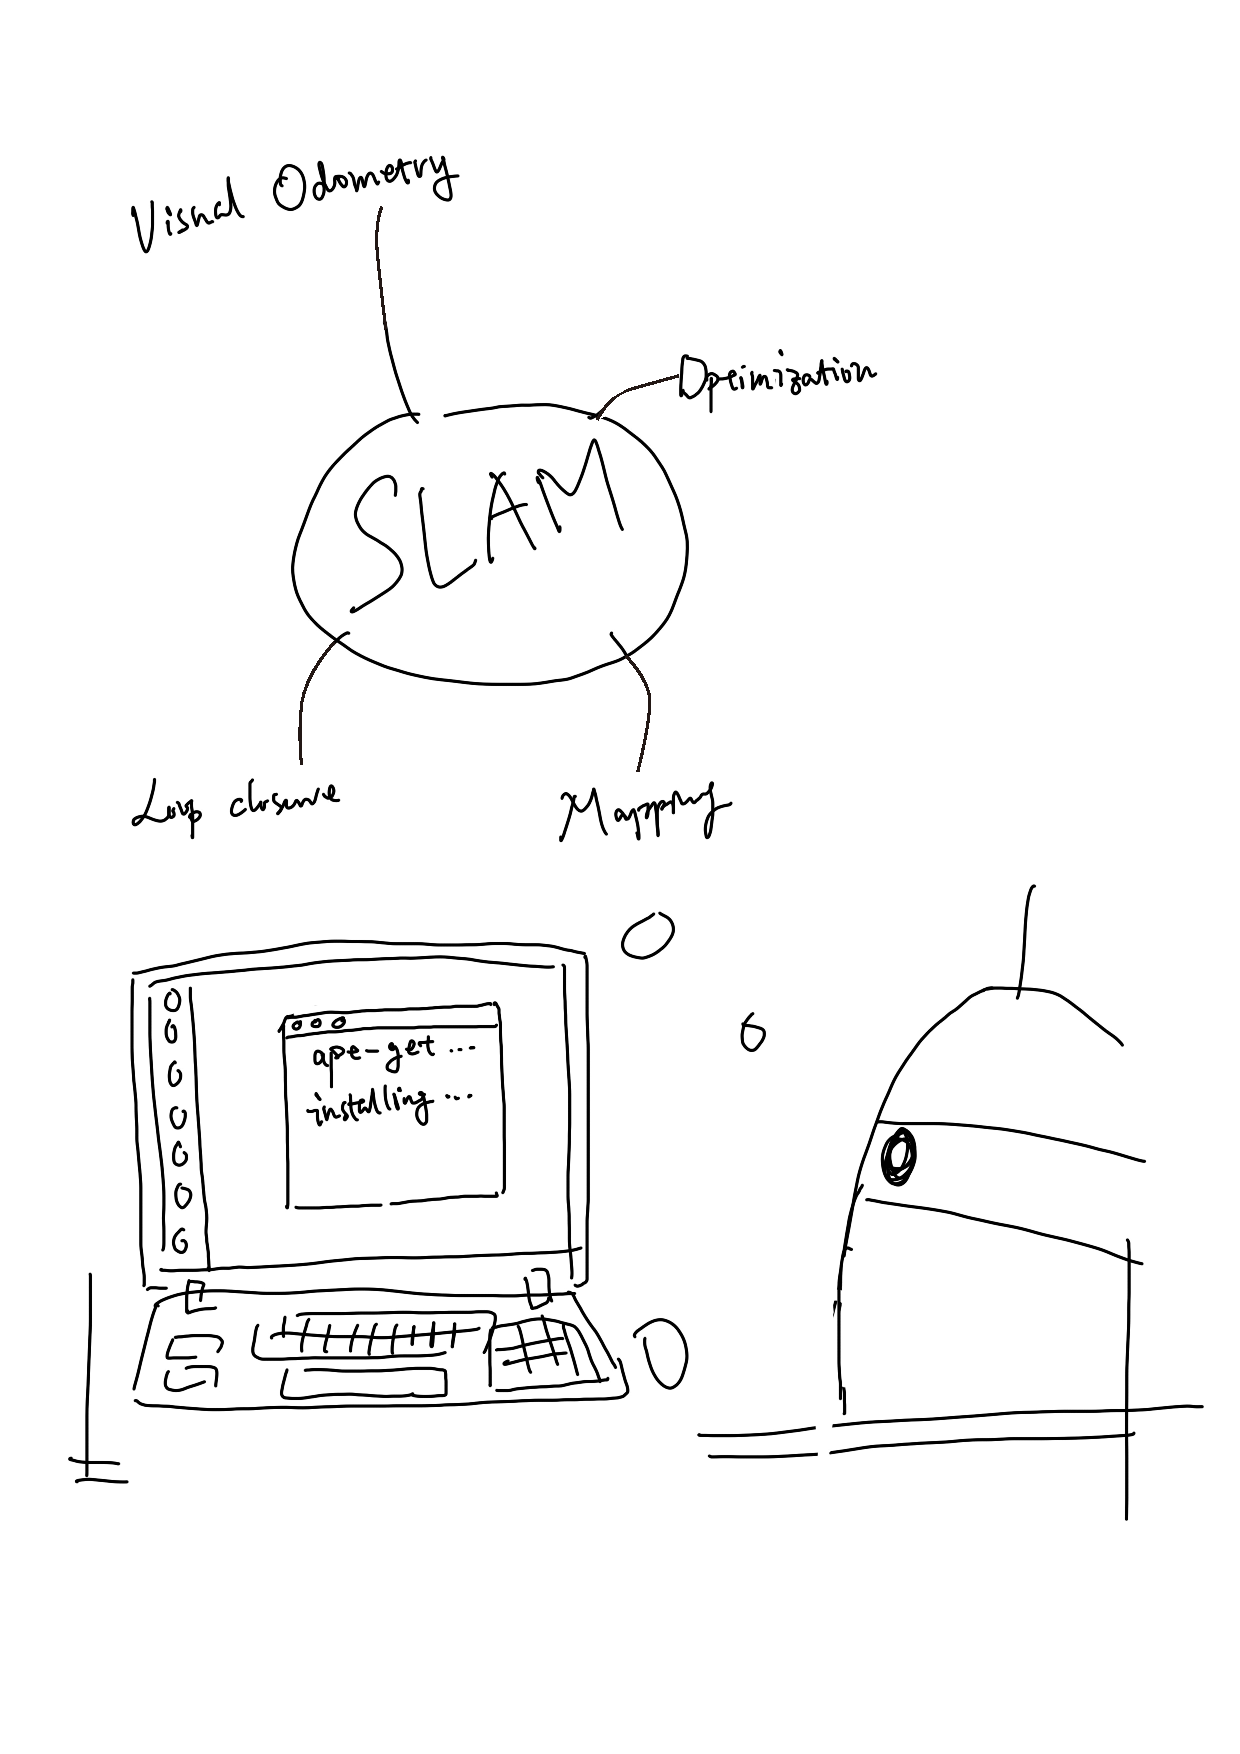
\includepdf{resources/other/ch2.pdf}
%\newpage

\section{Meet ``Little Carrot''}
Suppose we assembled a robot called \emph{Little Carrot}, as shown in the following figure:

\begin{figure}
	\centering
	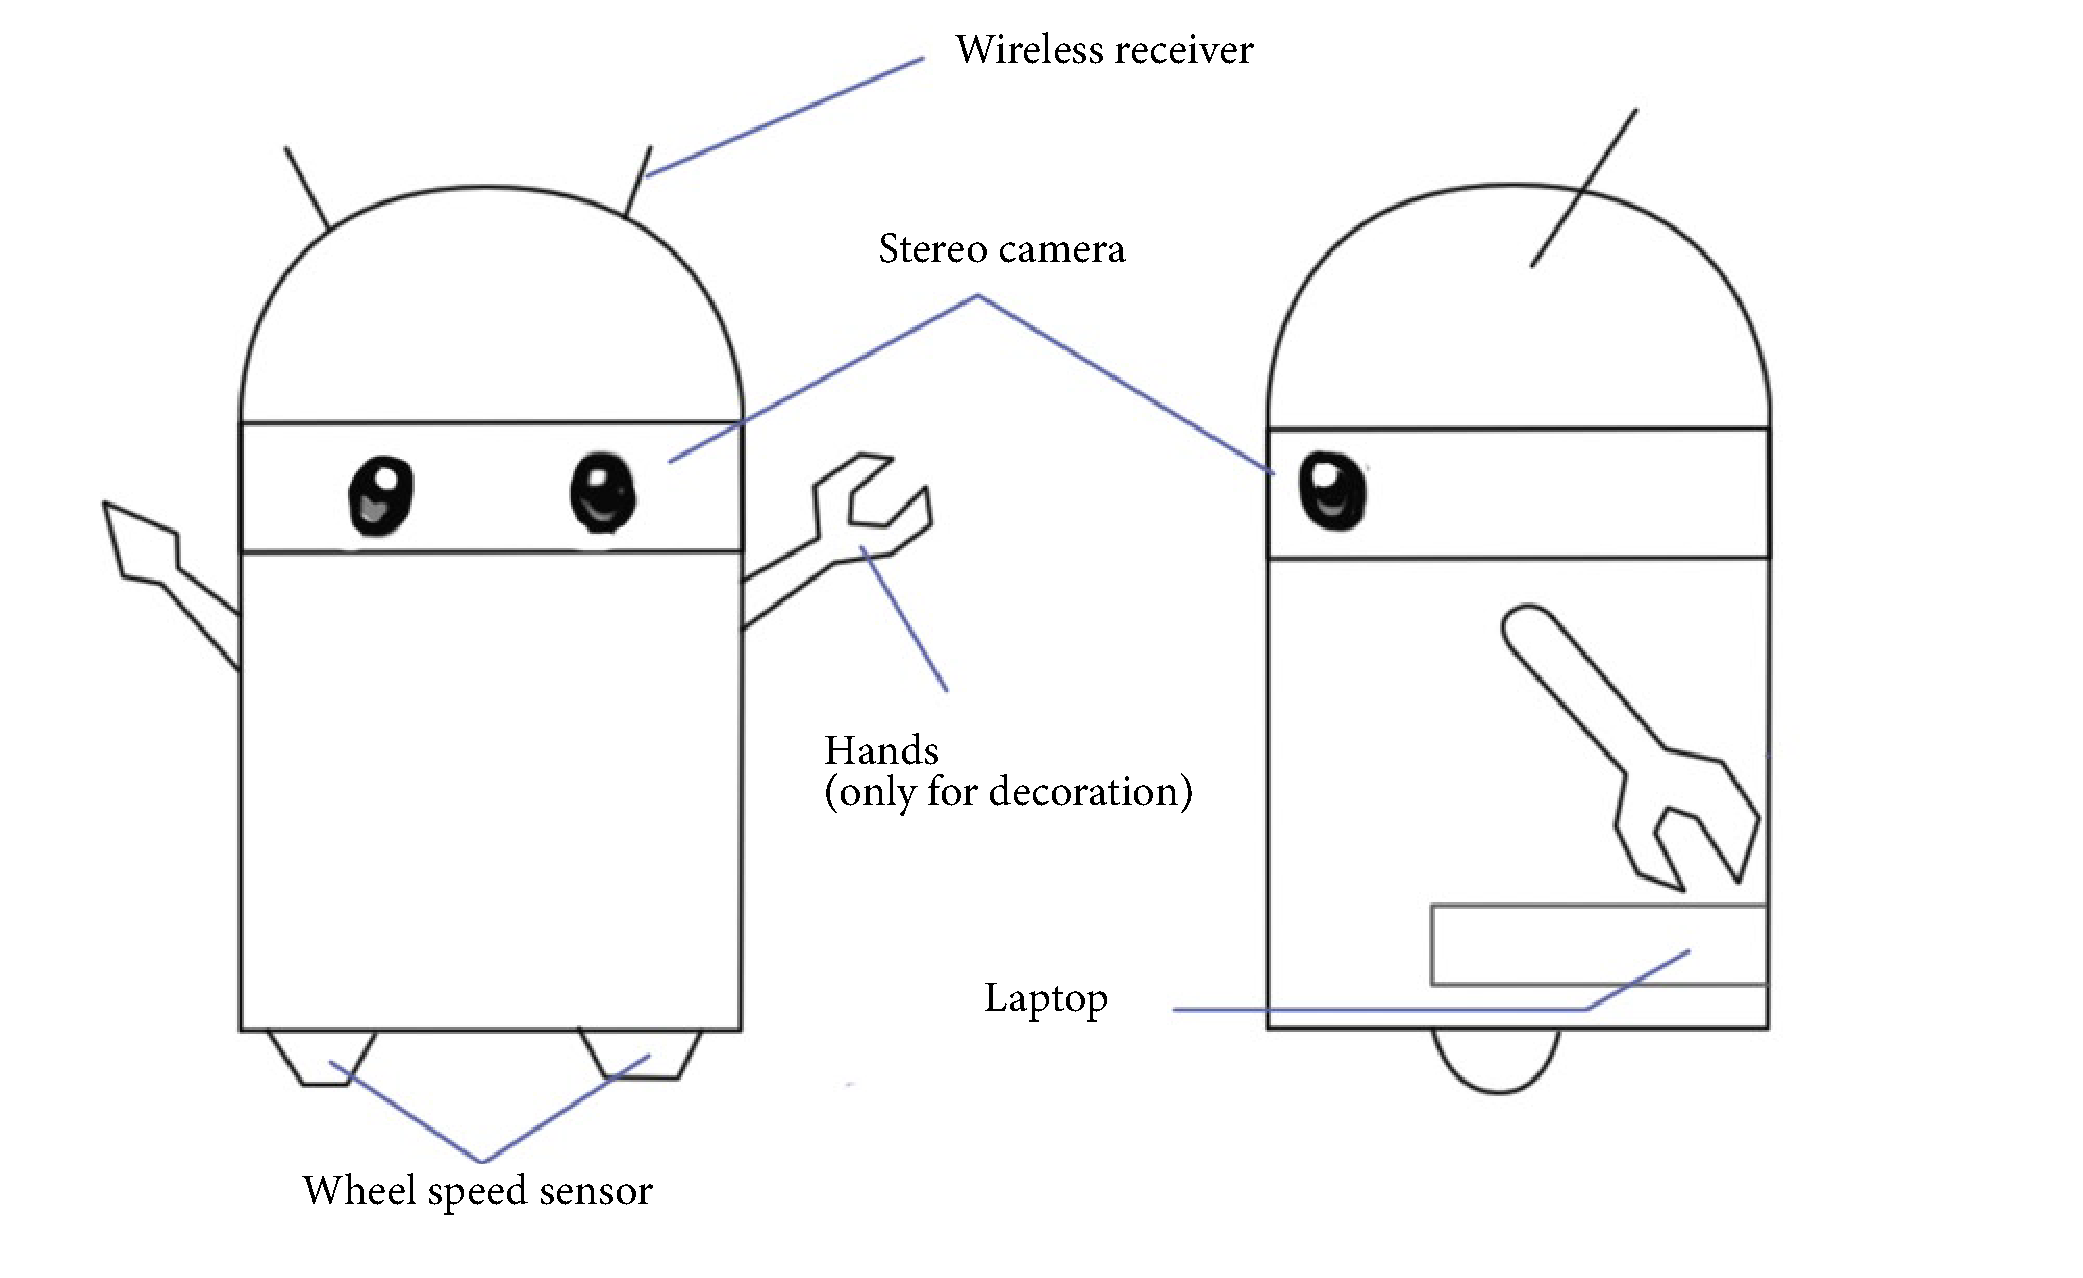
\includegraphics[width=0.8\textwidth]{resources/whatIsSLAM/carrot.pdf}
	\caption{The sketch of robot \emph{Little Carrot}}
\end{figure}

Although it looks a bit like the Android robot, it has nothing to do with the Android system. We put a laptop into its trunk (so that we can debug programs at any time). So, what do we expect it to do? 

We hope \textit{Little Carrot} has the ability of autonomous moving. Many domestic robots are placed statically on desktops. They can chat with people or play music, but a tablet computer nowadays can also deliver the same tasks. As a robot, we hope Little Carrot can move freely in a room. Wherever we say hello to it, it can come to us right away.

First of all, such a robot needs wheels and motors to move, so we installed wheels on it (gait control for humanoid robots is very complicated, which we will not be considered here). Now with the wheels, the robot is able to move, but without an effective navigation system, \textit{Little Carrot} does not know where a target of action is, and it can do nothing but wander around blindly. Even worse, it may hit a wall and cause damage. To avoid this, we installed cameras on its head, with the intuition that such a robot should look similar to a human. Indeed, with eyes, brains, and limbs, humans can walk freely and explore any environment, so we (somehow naively) think that our robot should be able to achieve it too. Well, to make Little Carrot able to explore a room, we find it at least needs to know two things:

\begin{enumerate}
	\item Where am I? - It's about \emph{localization}.
	\item What is the surrounding environment like? - It's about \emph{map building}.
\end{enumerate}

\textit{Localization} and \textit{map building} can be seen as the perception in both inward and outward directions. As a completely autonomous robot, \textit{Little Carrot} needs to understand its own state (i.e., the location) and the external environment (i.e., \ the map). Of course, there are many different approaches to solve these two problems. For example, we can lay guiding rails on the floor of the room, or paste a lot of artificial markers such as QR code pictures on the wall, or mount radio localization devices on the table. If you are outdoor, you can also install a GNSS receiver (like the one in a cell phone or a car) on the head of Little Carrot. With these devices, can we claim that the localization problem has been resolved? Let's categorize these sensors (see Fig.~\ref{fig:sensors}) into two classes.

\begin{figure}
	\centering
	\includegraphics[width=0.8\textwidth]{./resources/whatIsSLAM/sensors.jpg}
	\caption{Different kinds of sensors: (a) QR code; (b) GNSS receiver; (c) Guiding rails; (d) Laser range finder; (e) Inertial measurement unit; (f) Stereo camera; }
	\label{fig:sensors}
\end{figure}

The first class is non-intrusive sensors, which are entirely self-contained inside a robot, such as wheel encoders, cameras, laser scanners, etc. They do not assume a cooperative environment around the robot. The other class is intrusive sensors depending on a prepared environment, such as the above-mentioned guiding rails, QR codes, etc. Intrusive sensors can usually locate a robot directly, solving the localization problem in a simple and effective manner. However, since they require changes in the environment, the usage scope is often limited to a certain degree. For example, if there is no GPS signal or guiding rails cannot be laid, what should we do in those cases?

We can see that the intrusive sensors place certain constraints on the external environment. A localization system based on them can only function properly when those constraints are met in the real world. Otherwise, the localization approach cannot be carried out anymore, like GPS localization system normally doesn't work well in indoor environments. Therefore, although this type of sensor is reliable and straightforward, it does not work as a general solution. In contrast, non-intrusive sensors, such as laser scanners, cameras, wheel encoders, Inertial Measurement Units (IMUs), etc., can only observe indirect physical quantities rather than the direct location. For example, a wheel encoder measures the wheel rotation angle. An IMU measures the angular velocity and the acceleration. A camera or a laser scanner observes the external environment in a specific form like point-clouds and images. We have to apply algorithms to infer positions from these indirect observations. While this sounds like a roundabout tactic, the more obvious benefit is that it does not make any demands on the environment, making it possible for this localization framework to be applied to an unknown environment. Therefore, they are called self-localization in many research areas.

Looking back at the SLAM definitions discussed earlier, we emphasized an unknown environment in SLAM problems. In theory, we should not presume which environment the \textit{Little Carrot} will be used (but in reality, we will have a rough range, such as indoor or outdoor), which means that we can not assume that external sensors like GPS can work smoothly. Therefore, the use of portable non-intrusive sensors to achieve SLAM is our main focus. In particular, when talking about visual SLAM, we generally refer to \textit{cameras}' usage to solve the localization and map building problems.

Visual SLAM is the main subject of this book, so we are particularly interested in what the Little Carrot's eyes can do. The cameras used in SLAM are different from the commonly seen single-lens reflex (SLR) cameras. It is often much cheaper and does not carry an expensive lens. It shoots at the surrounding environment at a specific rate, forming a continuous video stream. An ordinary camera can capture images at 30 frames per second, while high-speed cameras can do faster. The camera can be roughly divided into three categories: monocular, stereo, and RGB-D, as shown by the following figure~\ref{fig:cameras}. Intuitively, a monocular camera has only one camera. A stereo camera has two. The principle of an RGB-D camera is more complicated. In addition to collecting color images, it can also measure the distance of the scene from the camera for each pixel. RGB-D devices usually carry multiple cameras and may adopt a variety of different working principles. In the fifth lecture, we will detail their working principles, and readers just need an intuitive impression for now. Some new special and emerging camera types can also be applied to SLAM, such as panorama camera~\cite{Pretto2011}, event camera~\cite{Rueckauer2016}. Although they are occasionally seen in SLAM applications, so far, they have not become mainstream. From the appearance, we can infer that Little Carrot seems to carry a stereo camera.

\begin{figure}
	\centering
	\includegraphics[width=0.8\textwidth]{./resources/whatIsSLAM/camera.pdf}
	\caption{Different kinds of cameras: monocular, RGB-D and stereo. }
	\label{fig:cameras}
\end{figure}

Now, let's take a look at the pros and cons of using different types of cameras for SLAM.

\subsubsection{Monocular Camera}

The SLAM system that uses only one camera is called Monocular SLAM. This sensor structure is particularly simple, and the cost is particularly low. Therefore the monocular SLAM has been very attractive to researchers. You must have seen the output data of a monocular camera: photo. Yes, what can we do with a single photo?

A photo is essentially a \textit{projection} of a scene onto a camera's imaging plane. It reflects a three-dimensional world in a two-dimensional form. Evidently, there is one dimension lost during this projection process: the so-called \textit{depth} (or distance). In a monocular case, we can not obtain the distance between objects in the scene and the camera by using a single image. Later, we will see that this distance is critical for SLAM. Because we humans have seen many photos, we formed a natural sense of distances for most scenes, helping us determine the distance relationship among the objects in the image. For example, we can recognize objects in the image and correlate them with their approximate size obtained from daily experience. The close objects will occlude the distant objects; the sun, the moon, and other celestial objects are infinitely far away; an object will have shadow if it is under sunlight. This common-sense can help us determine the distance of objects, but there are also certain cases that confuse us, and we can no longer distinguish the distance and proper size of an object. The following figure~\ref{fig:why-depth} shows an example. We can not determine whether the figures are real people or small toys purely based on the image itself. Unless we change our view angle, explore the three-dimensional structure of the scene. It may be a big but far away object, but it may also be a close but small object. They may appear to be the same size in an image due to the perspective projection effect.

\begin{figure}
	\centering
	\includegraphics[width=0.8\textwidth]{./resources/whatIsSLAM/why-depth.pdf}
	\caption{We cannot tell if the people are real humans or just small toys from a single image.}
	\label{fig:why-depth}
\end{figure}

Since the image taken by a monocular camera is just a 2D projection of the 3D space, if we want to recover the 3D structure, we have to change the camera's view angle. Monocular SLAM adopts the same principle. We move the camera and estimate its motion, as well as the distances and sizes of the objects in the scene, namely the structure of the scene. So how do we estimate these movements and structures? From the everyday experience, we know that if a camera moves to the right, the objects in the image will move to the left, which gives us an inspiration of inferring motion. On the other hand, we also know that closer objects move faster, while distant objects move slower. Thus, when the camera moves, the movement of these objects on the image forms pixel \textit{disparity}. Through calculating the disparity, we can quantitatively determine which objects are far away and which objects are close.

However, even if we know which objects are near and far, they are still only relative values. For example, when we are watching a movie, we can tell which objects in the movie scene are bigger than the others, but we can not determine the real size of those objects -- are the buildings real high-rise buildings or just models on a table? Is it a real monster that destroys a building, or just an actor wearing special clothing? Intuitively, if the camera's movement and the scene size are doubled simultaneously, monocular cameras see the same. Likewise, multiplying this size by any factor, we will still get the same picture. This demonstrates that the trajectory and map obtained from monocular SLAM estimation will differ from the actual trajectory and map with an unknown factor, which is called the \textit{scale} \footnote{We will explain the mathematical reason in the visual odometry chapter.}. Since monocular SLAM can not determine this real scale purely based on images, this is also called the scale ambiguity.

In monocular SLAM, depth can only be calculated with translational movement, and the real scale cannot be determined. These two things could cause significant trouble when applying monocular SLAM into real-world applications. The fundamental cause is that depth can not be determined from a single image. So, in order to obtain real-scaled depth, we start to use stereo and RGB-D cameras.

\subsubsection{Stereo Cameras and RGB-D Cameras}
The purpose of using stereo and RGB-D cameras is to measure the distance between objects and the camera, to overcome the shortcomings of monocular cameras that distances are unknown. Once distances are known, the 3D structure of a scene can be recovered from a single frame and eliminates scale ambiguity. Although both stereo and RGB-D cameras can measure the distance, their principles are not the same. A stereo camera consists of two synchronized monocular cameras, displaced with a known distance, namely the baseline. Because the physical distance of the baseline is known, we can calculate each pixel's 3D position in a very similar way to our human eyes. We can estimate the objects' distances based on the differences between the images from the left and right eye, and we can try to do the same on computers (see Fig.~\ref{fig:stereo}). We can also extend stereo camera to multi-camera systems if needed, but basically, there is no much difference.

\begin{figure}
    \centering
    \includegraphics[width=0.8\textwidth]{./resources/whatIsSLAM/stereo.pdf}
    \caption{Distance is calculated from the disparity of two stereo image pair.}
    \label{fig:stereo}
\end{figure}

Stereo cameras usually require a significant amount of computational power to (unreliably) estimate depth for each pixel, which is really clumsy compared to human beings. The depth range measured by a stereo camera is related to the baseline length. The longer a baseline is, the farther it can measure. So stereo cameras mounted on autonomous vehicles are usually quite big. Depth estimation for stereo cameras is achieved by comparing images from the left and right cameras and not relying on other sensing equipment. Thus stereo cameras can be applied both indoor and outdoor. The disadvantage of stereo cameras or multi-camera systems is that the configuration and calibration process is complicated. Their depth range and accuracy are limited by baseline length and camera resolution. Moreover, stereo matching and disparity calculation also consume many computational resources and usually require GPU or FPGA to accelerate to generate real-time depth maps. Therefore, in most state-of-the-art algorithms, the computational cost is still one of the major problems of stereo cameras.

Depth camera (also known as RGB-D camera, RGB-D will be used in this book) is a new type of camera rising since 2010. Similar to laser scanners, RGB-D cameras adopt infrared structure of light or Time-of-Flight (ToF) principles and measure the distance between objects and the camera by actively emitting light to the object and receive the returned light. This part is not solved by software as a stereo camera, but by physical sensors to save many computational resources compared to stereo cameras (see Fig.~\ref{fig:RGBD}). Common RGB-D cameras include Kinect / Kinect V2, Xtion Pro Live, RealSense, etc. However, most of the RGB-D cameras still suffer from issues including narrow measurement range, noisy data, small field of view, susceptibility to sunlight interference, and unable to measure transparent material. For SLAM purposes, RGB-D cameras are mainly used in indoor environments and are not suitable for outdoor applications \footnote{Note that this book is written in 2016. The statements may be outdated in future.}.

\begin{figure}
    \centering
    \includegraphics[width=0.8\textwidth]{./resources/whatIsSLAM/rgbd.pdf}
    \caption{RGBD cameras measure the distance and can build a point cloud with a single image frame.}
    \label{fig:RGBD}
\end{figure}

We have discussed the common types of cameras, and we believe you should have gained an intuitive understanding of them. Now, imagine a camera is moving in a scene, we will get a series of continuously changing images \footnote{You can try to use your phone to record a video clip.}. The goal of visual SLAM is to localize and build a map using these images. This is not a simple task like you think. It is not a single algorithm that continuously outputs positions and map information as long as we feed it with input data. SLAM requires an algorithm framework, and after decades of hard work by researchers, the framework has been matured in recent years.

\section{Classical Visual SLAM Framework}

Let's take a look at the classic visual SLAM framework, shown in the following figure~\ref{fig:workflow}:

\begin{figure}
    \centering
    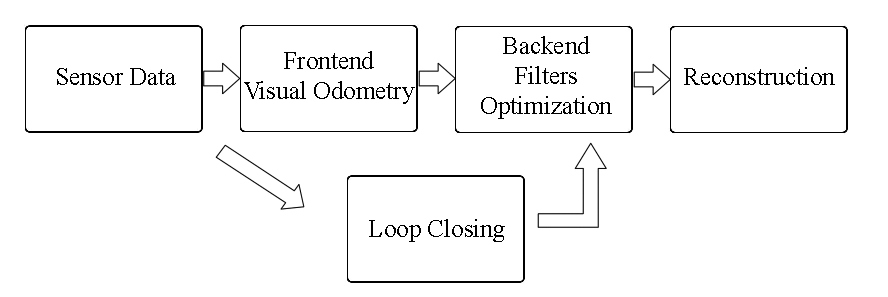
\includegraphics[width=0.8\textwidth]{./resources/whatIsSLAM/workflow.pdf}
    \caption{The classic visual SLAM framework.}
    \label{fig:workflow}
\end{figure}

A typical visual SLAM workflow  includes the following steps:
\begin{enumerate}
\item{Sensor data acquisition}. In visual SLAM, this mainly refers to for acquisition and preprocessing of camera images. For a mobile robot, this will also include the acquisition and synchronization with motor encoders, IMU sensors, etc.
\item{Visual Odometry (VO)}. VO's task is to estimate the camera movement between adjacent frames (ego-motion) and generate a rough local map. VO is also known as the \emph{frontend}.
\item{Backend filtering/optimization}. The backend receives camera poses at different time stamps from VO and results from loop closing, and then applies optimization to generate a fully optimized trajectory and map. Because it is connected after the VO, it is also known as the \textit{backend}.
\item {Loop Closing}. Loop closing determines whether the robot has returned to its previous position in order to reduce the accumulated drift. If a loop is detected, it will provide information to the backend for further optimization.
\item {Reconstruction}. It constructs a task-specific map based on the estimated camera trajectory.
\end{enumerate}

The classic visual SLAM framework is the result of more than a decade's research endeavor. The framework itself and the algorithms have been basically finalized and provided as essential functions in several public vision and robotics libraries. Relying on these algorithms, we can build visual SLAM systems performing real-time localization and mapping in static environments. Therefore, we can reach a rough conclusion that if the working environment is limited to fixed and rigid with stable lighting conditions and no human interference, the visual SLAM problem is basically solved~\cite{Cadena2016}.

The readers may not have fully understood the concepts of the modules mentioned above yet, so we will detail each module's functionality in the following sections. However, a deeper understanding of their working principles requires certain mathematical knowledge, which will be expanded in this book's second part. For now, an intuitive and qualitative understanding of each module is good enough.

\subsubsection{Visual Odometry}

The visual odometry is concerned with the movement of a camera between adjacent image frames, and the simplest case is, of course, the motion between two successive images. For example, when we see the images in Fig.~\ref{fig:cameramotion}, we will naturally tell that the right image should be the result of the left image after a rotation to the left with a certain angle (it will be easier if we have a video input). Let's consider this question: how do we know the motion is ``turning left''? Humans have long been accustomed to using our eyes to explore the world and estimating our own positions, but this intuition is often difficult to explain, especially in natural language. When we see these images, we will naturally think that, ok, the bar is close to us, the walls and the blackboard are farther away. When the camera turns to the left, the bar's closer part starts to appear, and the cabinet on the right side starts to move out of our sight. With this information, we conclude that the camera should be rotating to the left.

\begin{figure}
    \centering
    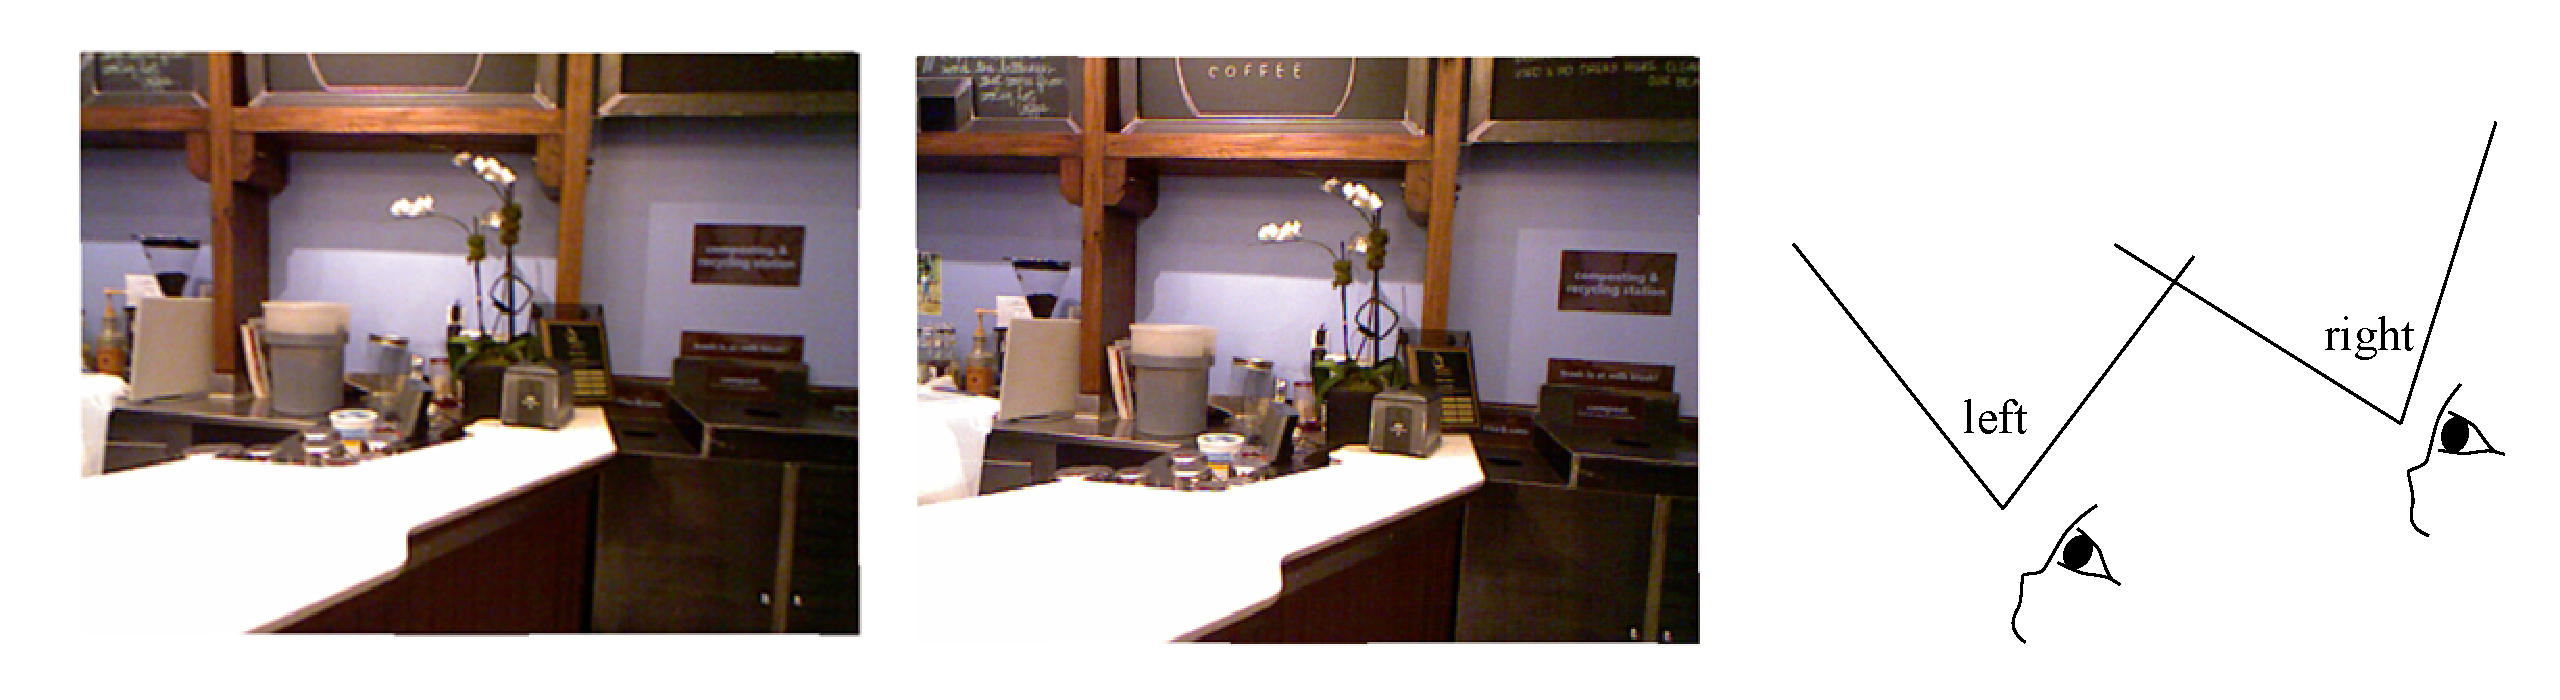
\includegraphics[width=1.0\textwidth]{./resources/whatIsSLAM/cameramotion.pdf}
    \caption{Camera motion can be inferred from two consecutive image frames. Images are from the NYUD dataset~\cite{Silberman2012}.}
    \label{fig:cameramotion}
\end{figure}

But if we go a step further: can we determine how much the camera has rotated or translated in units of degrees or centimeters? It is still difficult for us to give a quantitative answer. Because our intuition is not good at calculating numbers. But for a computer, movements have to be described with such numbers. So we will ask: how should a computer determine a camera's motion only based on images?

As mentioned earlier, in the field of computer vision, a task that seems natural to a human can be very challenging for a computer. Images are nothing but numerical matrices in computers. A computer has no idea what these matrices \textit{mean} (this is the problem that machine learning is also trying to solve). In visual SLAM, we can only see blocks of pixels, knowing that they are the results of projections by spatial points onto the camera's imaging plane. In order to quantify a camera's movement, we must first {understand the geometric relationship between a camera and the spatial points}.

Some background knowledge is needed to clarify this geometric relationship and the realization of VO methods. Here we only want to convey an intuitive concept. For now, you just need to take away that VO can estimate camera motions from images of adjacent frames and restore the 3D structures of the scene. It is named odometry because it is similar to a real wheel odometry, which only calculates the ego-motion at neighboring moments and does not estimate a global map or an absolute pose. In this regard, VO is like a species with only a short memory.

Now, assuming that we have the visual odometry, we are able to estimate camera movements between every two successive frames. If we connect the adjacent movements, this naturally constitutes the robot trajectory movement and addresses the localization problem. On the other hand, we can calculate the 3D position for each pixel according to the camera position at each time step, and they will form a map. Up to here, it seems with a VO, the SLAM problem is already solved. Or, is it?

Visual odometry is indeed a key technology for solving the visual SLAM problem. We will be spending a significant part explaining it in detail. However, using only a VO to estimate trajectories will inevitably cause {accumulative drift}. This is because the visual odometry (in the simplest case) only estimates the movement between two frames. We know that each estimate is accompanied by a certain error. Because of the way odometry works, errors from previous moments will be carried forward to the next moments, resulting in inaccurate estimation after some time (see Fig.~\ref{fig:loopclosure}). For example, the robot first turns left 90$^\circ$ and then turns right 90$^\circ$. Due to error, we estimate the first 90$^\circ$ as 89$^\circ$, which is possible to happen in real-world applications. Then we will be embarrassed to find that after the right turn, the robot's estimated position will not return to the origin. What's worse, even the following estimates are perfectly calculated, they will always be carrying this 1$^\circ$ error compared to the true trajectory.

\begin{figure}
    \centering
    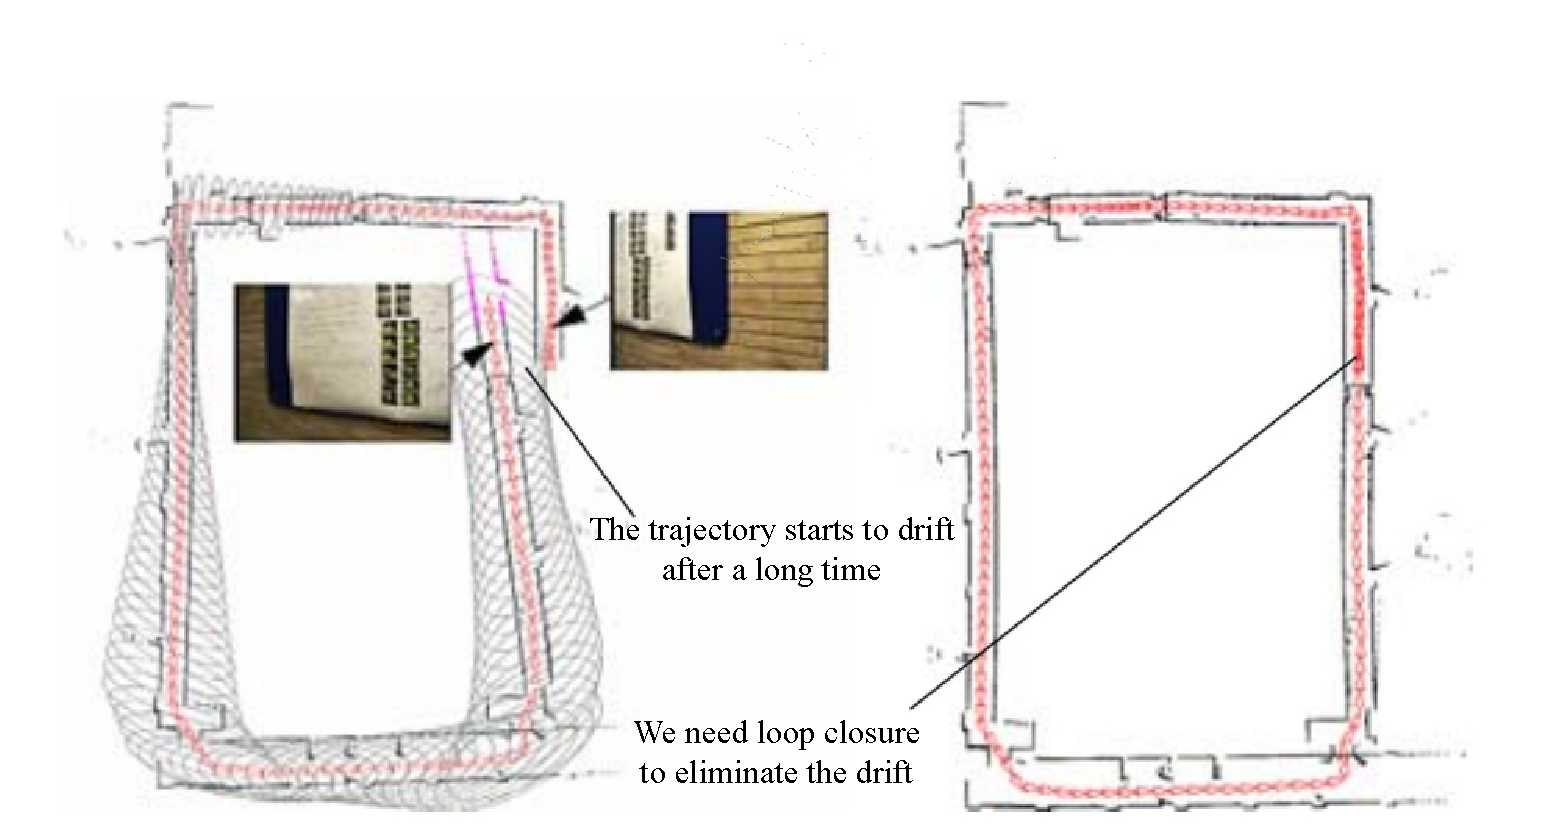
\includegraphics[width=1.0\textwidth]{./resources/whatIsSLAM/loopclosure.pdf}
    \caption{Drift will be accumulated if we only have a relative motion estimation~\cite{Ho2007}.}
    \label{fig:loopclosure}
\end{figure}

The accumulated drift will make us unable to build a consistent map. A straight corridor may oblique, and a 90$^\circ$ angle may be crooked - this is really an unbearable matter! To solve the drifting problem, we also need other two components: the \textit{backend optimization} \footnote{It is usually known as the \textit{backend}. Since it is often implemented by optimization, so we use the term backend optimization.} and \textit{loop closing}. Loop closing is responsible for detecting whether the robot returns to its previous position, while the backend optimization corrects the shape of the entire trajectory based on this information.

\subsubsection{Backend Optimization}
Generally speaking, backend optimization mainly refers to the process of dealing with the \emph{noise} in SLAM systems. We hope that all the sensor data is accurate, but in reality, even the most expensive sensors still have a certain amount of noise. Cheap sensors usually have larger measurement errors, while that of expensive ones may be small. Moreover, many sensors' performance is affected by changes in the magnetic field, temperature, etc. Therefore, in addition to solving the problem of estimating camera movements from images, we also care about how much noise this estimation contains, how it is carried forward from the last time step to the next, and how confident we have in the current estimation. The backend optimization solves the problem of estimating the state of the entire system from noisy input data and calculate their uncertainty. The state here includes both the robot's own trajectory and the environment map.

In contrast, the visual odometry part is usually referred to as the \textit{frontend}. In a SLAM framework, the frontend provides data to be optimized by the backend and the initial values. Because the backend is responsible for the overall optimization, we only care about the data itself instead of where it comes from. In other words, we only have numbers and matrices in the backend without those beautiful images. In visual SLAM, the frontend is more relevant to \textit{computer vision} topics, such as image feature extraction and matching, while the backend is relevant to the \textit{state estimation} research area.

Historically, the backend optimization part has been equivalent to ``SLAM research'' for a long time. In the early days, the SLAM problem was described as a state estimation problem, exactly what the backend optimization tries to solve. In the earliest papers on SLAM, researchers at that time called it ``estimation of spatial uncertainty''~\cite{Smith1986, Smith1990}. Although it sounds a little obscure, it does reflect the nature of the SLAM problem: the estimation of the uncertainty of the self-movement and the surrounding environment. In order to solve the SLAM problem, we need state estimation theory to express the uncertainty of localization and map construction and then use filters or nonlinear optimization to estimate the mean and uncertainty (covariance) of the states. The details of state estimation and nonlinear optimization will be explained in chapter~\ref{cpt:6},~\ref{cpt:backend1}, and~\ref{cpt:backend2}.

\subsubsection{Loop Closing}
Loop Closing, also known as \textit{loop closure detection}, mainly addresses the drifting problem of position estimation in SLAM. So how to solve it? Assuming a robot has returned to origin after a movement period, the estimated does not return to the origin due to drift. How to correct it? Imagine that if there is some way to let the robot know that it has returned to the origin, we can pull the estimated locations to the origin to eliminate drifts, which is what the loop closing exactly does.

Loop closing has a close relationship with both localization and map building. In fact, the main purpose of building a map is to enable a robot to know the places it has been to. To achieve loop closing, we need to let the robot have the ability to identify the scenes it has visited before. There are different alternatives to achieve this goal. For example, as we mentioned earlier, we can set a marker where the robot starts, such as a QR code. If the sign was seen again, we know that the robot has returned to the origin. However, the marker is essentially an intrusive sensor that sets additional constraints to the application environment. We prefer the robot can use its non-intrusive sensors, e.g., the image itself, to complete this task. A possible approach would be to detect similarities between images. This is inspired by us humans. When we see two similar images, it is easy to identify that they are taken from the same place. If the loop closing is successful, the accumulative error can be significantly reduced. Therefore, visual loop detection is essentially an algorithm for calculating similarities of images. Note that the loop closing problem also exists in laser-based SLAM. The rich information contained in images can remarkably reduce the difficulty of making a correct loop detection.

After a loop is detected, we will tell the backend optimization algorithm like, ``OK,  A and B are the same point''. Based on this new information, the trajectory and the map will be adjusted to match the loop detection result. In this way, if we have sufficient and reliable loop detection, we can eliminate cumulative errors and get globally consistent trajectories and maps.

\subsubsection{Mapping}
Mapping means the process of building a map, whatever kind it is. A map (see Fig.~\ref{fig:mapping}) is a description of the environment, but the way of description is not fixed and depends on the actual application.

\begin{figure}
	\centering
	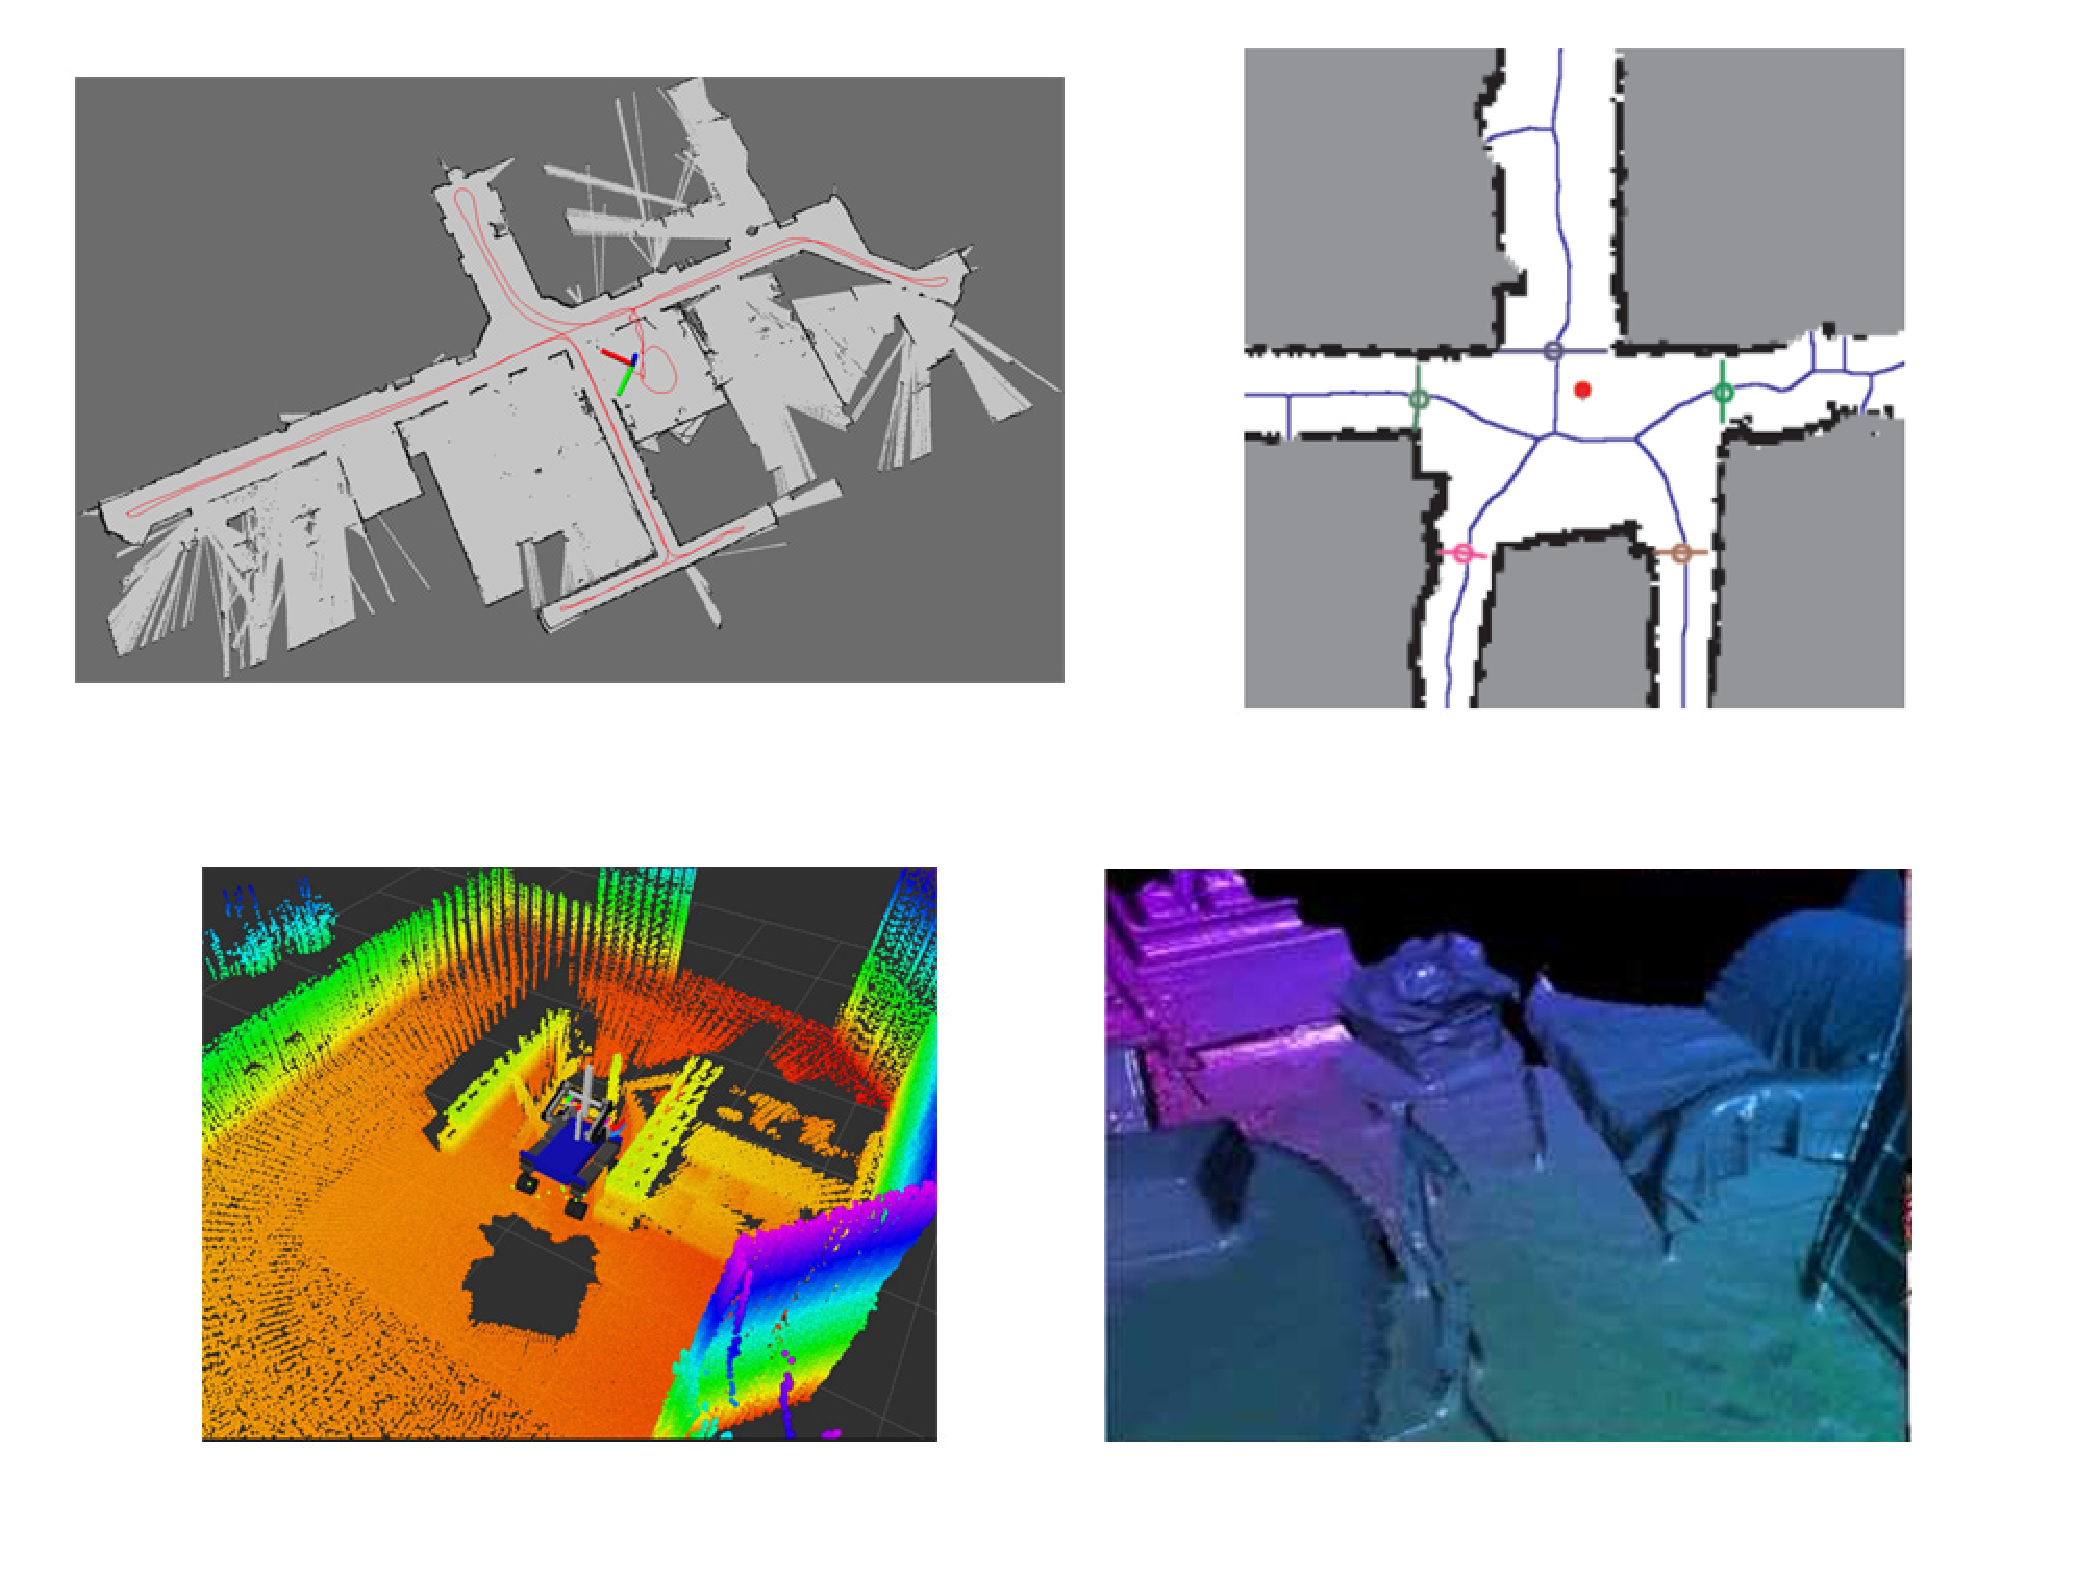
\includegraphics[width=1.0\textwidth]{./resources/whatIsSLAM/map.pdf}
	\caption{Different kinds of maps: 2D grid map, 2D topological map, 3D point clouds and 3D meshes~\cite{Beeson2010}.}
	\label{fig:mapping}
\end{figure}

Let's take the domestic cleaning robots as an example. Since they basically move on the ground, a two-dimensional map with marks for open areas and obstacles, built by a single-line laser scanner, would be sufficient for navigation for them. And for a camera, we need at least a three-dimensional map for its 6 degrees-of-freedom movement. Sometimes, we want a smooth and beautiful reconstruction result, not just a set of points but also a texture of triangular faces. And at other times, we do not care about the map, just need to know things like ``point A and point B are connected, while point B and point C are not'', which is a topological way to understand the environment. Sometimes maps may not even be needed. For instance, a level-2 autonomous driving car can make a lane-following driving only knowing its relative motion with the lanes.

For maps, we have various ideas and demands. Compared to the previously mentioned VO, loop closure detection, and backend optimization, map building does not have a particular algorithm. A collection of spatial points can be called a map. A beautiful 3D model is also a map, so is a picture of a city, a village, railways, and rivers. The form of the map depends on the application of SLAM. In general, they can be divided into to categories: \emph{metrical maps} and \emph{topological maps}.

\paragraph{Metric Maps}
Metrical maps emphasize the exact metrical locations of the objects in maps. They are usually classified as either sparse or dense. Sparse metric maps store the scene into a compact form and do not express all the objects. For example, we can construct a sparse map by selecting representative landmarks such as the lanes and traffic signs and ignore other parts. In contrast, dense metrical maps focus on modeling all the things that are seen. A sparse map would be enough for localization, while for navigation, a dense map is usually needed (otherwise, we may hit a wall between two landmarks). A dense map usually consists of a number of small grids at a certain resolution. It can be small occupancy grids for 2D metric maps or small voxel grids for 3D maps. For example, in a 2D occupancy grid map, a grid may have three states: occupied, not occupied, and unknown, to express whether there is an object. When a spatial location is queried, the map can provide information about whether the location is passable. This type of maps can be used for various navigation algorithms, such as A$^*$, D$^*$\footnote{ See \url{https://en.wikipedia.org/wiki/A*_search_algorithm}.}, etc., and thus attract the attention of robotics researchers. But we can also see that all the grid status are store in the map, thus being storage expensive. There are also some open issues in building a metric map. For example, in large-scale metrical maps, a small steering error may cause the walls of two rooms to overlap, making the map ineffective.

\paragraph{Topological Maps}
Compared to the accurate metrical maps, topological maps emphasize the relationships among map elements. A topological map is a graph composed of nodes and edges, only considering the connectivity between nodes. For instance, we only care about that point A and point B are connected, regardless of how we could travel from point A to point B. It relaxes the requirements on precise locations of a map by removing map details and is, therefore, a more compact expression. However, topological maps are not good at representing maps with complex structures. Questions such as how to split a map to form nodes and edges and how to use a topological map for navigation and path planning are still open problems to be studied.

\section{Mathematical Formulation of SLAM Problems}
Through the previous introduction, readers should have gained an intuitive understanding of the modules in a SLAM system and each module's main functionality. However, we cannot write runnable programs only based on intuitive impressions. We want to raise it to a rational and rigorous level, using mathematical symbols to formulate a SLAM process. We will be using variables and formulas, but please rest assured that we will try our best to keep it clear enough.

Assuming that our Little Carrot is moving in an unknown environment, carrying some sensors. How can this be described in mathematical language? First, since sensors usually collect data at different time points, we are only concerned with the locations and the map at these moments. This turns a continuous process into discrete time steps, say $1, \cdots, k$, at which data sampling happens. We use $\mathbf{x}$ to indicate positions of Little Carrot. So the positions at different time steps can be written as $\mathbf{x}_1,\cdots,\mathbf{x}_k$, which constitute the trajectory of Little Carrot. In terms of the map, we assume that the map is made up of several \emph{landmarks}, and at each time step, the sensors can see a part of the landmarks and record their observations. Assume there is a total of $N$ landmarks in the map, and we will use $\mathbf{y}_1, \cdots, \mathbf{y}_N$ to denote them.

With such a setting, the process that \textit{Little Carrot moves in the environment with sensors} basically has two parts: 

\begin{enumerate}
\item What is its \emph{motion}? We want to describe how $\mathbf{x}$ changes from time step $k-1$ to $k$.
\item What are the sensor \emph{observations}? Assuming that the Little Carrot detects a specific landmark, let's say $\mathbf{y}_j$ at position $\mathbf{x}_k$, we need to describe this event in mathematical language.
\end{enumerate}

Let's first take a look at motion. Typically, we may send some motion commands to the robots like ``turn 15 degrees to left''. These commands will be finally carried out by the controller, probably in many different ways. Sometimes we control the position of robots, but acceleration or angular velocity would always be reasonable alternates. However, no matter what the controller is, we can use a universal and abstract mathematical model to describe it:
\begin{equation}
{\mathbf{x}_k} = f\left( {{\mathbf{x}_{k - 1}},{\mathbf{u}_k}, \mathbf{w}_k} \right),
\end{equation}
where $\mathbf{u}_k$ is the input commands, and $\mathbf{w}_k$ is noise. Note that we use a general $f(\cdot)$ to describe the process, instead of specifying the exact form of $f$. This allows the function to represent any motion input, rather than being limited to a particular one. We call it the \emph{motion equation}.

The presence of noise turns this model into a stochastic model. In other words, even if we give an order as ``move forward one meter'', it does not mean that our robot really drives one meter in front. If all the instructions are accurate, there is no need to estimate anything. In fact, the robot may only forward by, say, 0.9 meters, and at another moment, it moves by 1.1 meters. Thus, the noise during each movement is random. If we ignore this noise, the position determined only by the input command maybe a hundred miles away from the real position after several minutes.

Corresponding to the motion equation, we also have an \textit{observation equation}. The observation equation describes the process that the Little Carrot sees a landmark point $\mathbf{y}_j$ at $\mathbf{x}_k$ and generates an observation data $\mathbf{z}_{k,j}$. Likewise, we will describe this relationship with an abstract function $h(\cdot)$:
\begin{equation}
{\mathbf{z}_{k,j}} = h\left( {{\mathbf{y}_j},{\mathbf{x}_k}, \mathbf{v}_{k,j} } \right),
\end{equation}
where $\mathbf{v}_{k,j}$ is the noise in this observation. Since there are various observation sensors, the observed data $\mathbf{z}$ and the observation equation $h$ may also have many different forms.

Readers may say that the function $f,h$ here does not seem to specify what is going on in the motion and observation. Also, what do the variables $\mathbf{x}$, $\mathbf{y}$, $\mathbf{z}$ mean here? Depending on the actual motion and the type of sensor, there are several kinds of parameterization methods. What is parameterization? For example, suppose our robot moves in a plane, then its pose \footnote{ In this book, we use the word ``pose'' to mean ``position'' plus ``rotation''. } is described by two $x-y$ coordinates and an angle, i.e.,  $\mathbf{x}_k = [x_1,x_2,\theta]_k^\mathrm{T}$, where $x_1, x_2$ are positions on two axes and $\theta$ is the angle. At the same time, the input command is the position and angle change between the time interval: $\mathbf{u}_k = [ \Delta x_1, \Delta x_2, \Delta \theta ]_k^\mathrm{T} $, so the motion equation can be parameterized as:
\begin{equation}
{\left[ \begin{array}{l}
    x_1\\
    x_2\\
    \theta
    \end{array} \right]_k} = {\left[ \begin{array}{l}
    x_1\\
    x_2\\
    \theta
    \end{array} \right]_{k - 1}} + {\left[ \begin{array}{l}
    \Delta x_1\\
    \Delta x_2\\
    \Delta \theta
    \end{array} \right]_k} + {\mathbf{w}_k},
\end{equation}
where $\mathbf{w}_k$ is the noise again. This is a simple linear relationship. However, not all input commands are position and angular changes. For example, the input of ``throttle'' or ``joystick'' is the speed or acceleration, so there are other forms of more complex motion equations. At that time, we would say the kinetic analysis is required.

Regarding the observation equation, for example, the robot carries a two-dimensional laser sensor. We know that a laser observes a 2D landmark by measuring two quantities: the distance $r$ between the landmark point and the robot, and the angle $\phi$. Let's say the landmark is at $\mathbf{y}_j = [y_1, y_2]_j^\mathrm{T}$, the pose is $\mathbf{x}_k=[x_1,x_2]_k^\mathrm{T}$, and the observed data is $\mathbf{z}_{k,j} = [r_{k,j}, \phi_{k,j}]^\mathrm{T}$, then the observation equation is written as:
\begin{equation}
\left[ \begin{array}{l}
r_{k,j}\\
\phi_{k,j}
\end{array} \right] = \left[ \begin{array}{l}
\sqrt {{{\left(y_{1,j} - x_{1,k} \right)}^2} + {{\left( {{y_{2,j}} - x_{2,k} } \right)}^2}} \\
\arctan \left( \frac{{y_{2,j}} - x_{2,k}}{{y_{1,j} - x_{1,k}}} \right)
\end{array} \right] + \mathbf{v}_{k, j}.
\end{equation}

When considering visual SLAM, the sensor is a camera, then the observation equation is a process like ``getting the pixels in the image of the landmarks.'' This process involves a description of the camera model, which will be covered in detail in chapter~\ref{cpt:5}.

Obviously, it can be seen that the two equations have different parameterized forms for different sensors. If we maintain versatility and take them into a common abstract form, then the SLAM process can be summarized into two basic equations:
\begin{equation}
\label{eq:slamproblem}
\left\{ \begin{array}{l}
{\mathbf{x}_k} = f\left( {{\mathbf{x}_{k - 1}},{\mathbf{u}_k}}, \mathbf{w}_k \right),\quad k=1,\cdots, K\\
{\mathbf{z}_{k,j}} = h\left( {{ \mathbf{y}_j},{ \mathbf{x}_k}}, \mathbf{v}_{k,j} \right), \quad (k,j) \in \mathcal{O}
\end{array} \right. ,
\end{equation}
where $\mathcal{O}$ is a set that contains the information at which pose the landmark was observed (usually not all the landmarks can be seen at every moment -- we are likely to see only a small part of the landmarks  at a single moment). These two equations together describe a basic SLAM problem: how to solve the estimate $\mathbf{x}$ (localization) and $\mathbf{y}$ (mapping) problem with the noisy control input $\mathbf{u}$ and the sensor reading $\mathbf{z}$ data? Now, as we see, we have modeled the SLAM problem as a \textbf{state estimation problem}: How to estimate the internal, hidden state variables through the noisy measurement data?

The solution to the state estimation problem is related to the two equations' specific form and the noise probability distribution. Whether the motion and observation equations are \textit{linear} and whether the noise is assumed to be \textit{Gaussian}, it is divided into \textbf{linear/nonlinear} and \textbf{Gaussian/non-Gaussian} systems. The Linear Gaussian (LG system) is the simplest, and its unbiased optimal estimation can be given by the Kalman Filter (KF). In the complex nonlinear non-Gaussian (NLNG system), we basically rely on two methods: Extended Kalman Filter (EKF) and nonlinear optimization. Until the early 21st century, the EKF-based filter method still dominated SLAM. We will linearize the system at the working point and solve it in two steps: predict-update (see chapter~\ref{cpt:backend1}). The earliest real-time visual SLAM system was developed based on EKF {\cite{Davison2007}}. Subsequently, in order to overcome the shortcomings of EKF (such as the linearization error and noise Gaussian distribution assumptions), people began to use other filters such as particle filters, and even use nonlinear optimization methods. Today, the mainstream of visual SLAM uses state-of-the-art optimization techniques represented by \textit{graph optimization} {\cite{Strasdat2012}}. We believe that optimization methods are clearly superior to filters, and as long as computing resources allow, optimization methods are often preferred (see chapters~\ref{cpt:backend1} and~\ref{cpt:backend2}).

Now we believe the reader has a general understanding of SLAM's mathematical model, but we still need to clarify some issues. First, we should explain what the \textit{pose} $\mathbf{x}$ is. The word \textit{pose} we just said is somewhat vague. Perhaps the reader can understand that a robot moving in the plane can be parameterized by two coordinates plus an angle. However, more robots are more like things in three-dimensional space. We know that the motion of the three-dimensional space consists of three axes, so the movement of the robot is described by the translation on the three axes and the rotation around the three axes, totally having six \textit{degrees of freedom} (DoF). But wait, does that mean that we can describe it with a vector in $\mathbb{R}^6$? We will find that things are not that simple. For a 6 DoF \textbf{pose}, how to express it? How to optimize it? How to describe its mathematical properties?  This will be the main content of the chapter~\ref{cpt:3} and~\ref{cpt:4}. Next, we will explain how the \textit{observation equation} is parameterized in the visual SLAM. In other words, how the landmark points in space are projected onto a photo? This requires an explanation of the camera's projection model and distortion, which we will cover in chapter~\ref{cpt:5}. Finally, when we know this information, how to solve the above state estimation problem? This requires knowledge of nonlinear optimization and is the content of chapter~\ref{cpt:6}.
    
These contents form part of the mathematical knowledge of this book. After laying the groundwork for them, we can discuss more detailed knowledge of visual odometry, backend optimization, and more. It can be seen that the content of this lecture constitutes a summary of the book. If you don't understand the above concepts well, you may want to go back and read them again. Now let's start the introduction of programming!

\section{Practice: Basics}
\subsection{Installing Linux}
Finally, we come to the exciting practice session! Are you ready? In order to complete the practice of this book, we need to prepare a computer. You can use a laptop or desktop, preferably your personal computer, because we need to install an operating system on it for experiments.

Our program is based on C++ programs on Linux. During the experiment, we will use several open-source libraries. Most libraries are only supported in Linux, while configuration on Windows is relatively (or quite) troublesome. Therefore, we have to assume that you already have a basic knowledge of Linux (see the previous lecture exercises), including using basic commands to understand how to install the software. Of course, you don't have to know how to develop C++ programs under Linux, which is what we want to talk about below.

Let's start by installing the experimental environment required for this book. As a book for beginners, we recommend Ubuntu as a development environment. Ubuntu and its variances have enjoyed a good reputation as a novice user in all major Linux distributions. Ubuntu is an open-source operating system. Its system and software can be downloaded freely on the official website (\url{http://ubuntu.com}), which provides detailed installation instructions. At the same time, Tsinghua University, China Science and Technology University, and other major universities in China have also provided Ubuntu software mirrors, making the software installation very convenient (probably there are also mirror websites in your country).

The first version of this book uses Ubuntu 14.04 as the default development environment. In the second edition, we updated the default version to the newer \textbf{Ubuntu 18.04} (\autoref{fig:ubuntu1804}) for later research. If you want to change the styles, then Ubuntu Kylin, Debian, Deepin, and Linux Mint are also good choices. I promise that all the code in the book has been well tested under Ubuntu 18.04, but if you choose a different distribution, I am not sure if you will encounter some minor problems. You may need to spend some time solving small issues (but you can also take them as opportunities to exercise yourself). In general, Ubuntu's support for various libraries is relatively complete and rich. Although we don't limit which Linux distribution you use, in the explanation, \textbf{we will use Ubuntu 18.04 as an example} and mainly use Ubuntu commands (such as apt-get). So, in other versions of Ubuntu, there will be no obvious differences below. In general, the migration of programs between Linux is not very difficult. But if you want to use the programs in this book under Windows or OS X, you need to have some porting experience.

\begin{figure}[!ht]
    \centering
    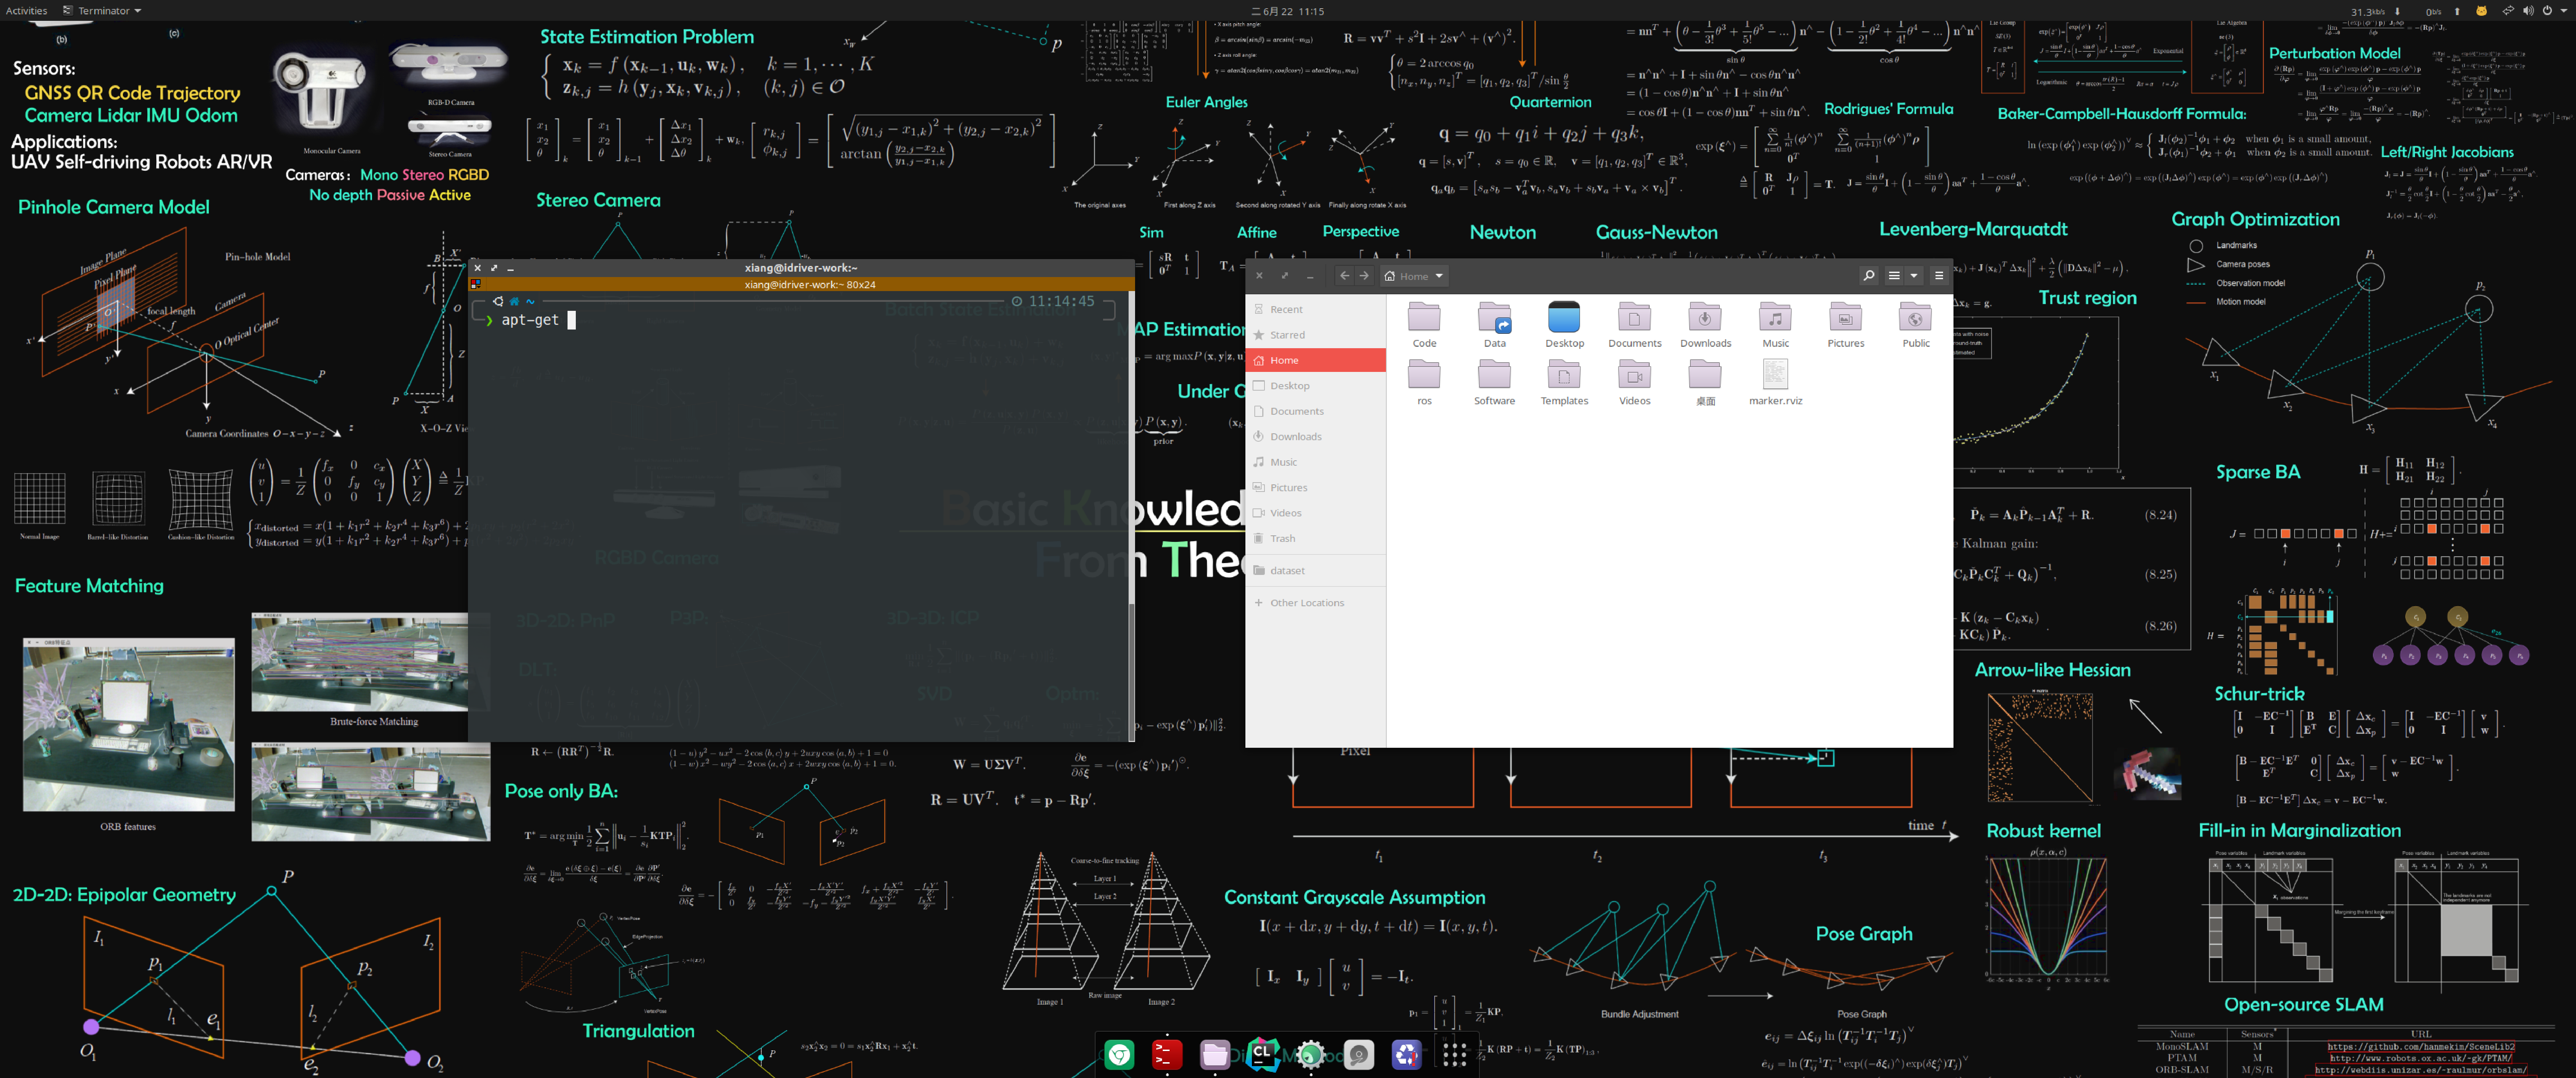
\includegraphics[width=1.0\textwidth]{whatIsSLAM/ubuntu.pdf}
    \caption{Ubuntu 18.04 in virtual machine.}
    \label{fig:ubuntu1804}
\end{figure}

Now, I assume there's an Ubuntu 18.04 installed on your PC. Regarding the installation of Ubuntu, you can find a lot of tutorials on the Internet. Just do it. I'll skip here. The easiest way is to use a virtual machine (see \autoref{fig:ubuntu1804}), but it takes a lot of memory (our experience is more than 4GB) and CPU to be smooth. You can also install dual systems, which will be faster, but a blank USB flash drive is required as the boot disk. In addition, virtual machine software support for external hardware is often not good enough. If you want to use real sensors (cameras, Kinects, etc.), it is recommended that you use dual systems to install Linux.

Now, let's say you have successfully installed Ubuntu, either a virtual machine or a dual system. If you are not familiar with Ubuntu, try its various software and experience its interface and interaction mode \footnote{Most people think Ubuntu is cool for the first time. }. But I have to remind you, especially to the novice friends: don't spend too much time on Ubuntu's user interface. Linux has a lot of chances to waste your time. You may find some niche software, some games, and even spend a lot of time looking for wallpapers. But remember, you are working with Linux. Especially in this book, you are using Linux to learn SLAM, so try to spend your time learning SLAM.

Ok, let's choose a directory and put the code for the SLAM program in this book. For example, you can put the code under \textit{slambook2} in the home directory (/home/username). We will refer to this directory \textit{code root} in the future. At the same time, you can choose another directory to copy the git code of this book, which is convenient for comparison when doing experiments. The code for this book is divided into chapters. For example, this chapter's code will be under slambook2/ch2, and the next one will be under slambook2/ch3. So, now please go into the slambook2/ch2 directory (you should create a new folder and enter the folder name).

\subsection{Hello SLAM}
Like many computer books, let's write a \textit{HelloSLAM} program. But before we do this, let's talk about what a program is.

In Linux, a program is a file with execute permissions. It can be a script or a binary file, but we don't limit its suffix name (unlike Windows, you need to specify it as a .exe file). The commonly used binaries such as \textit{cd} and \textit{ls} are executable files located in the \textit{/bin} directory. For an executable program elsewhere, as long as it has executable permissions, it will run when we enter the program name in the terminal. When programming in C++, we first write a text file:

\begin{lstlisting}[language=C++,caption=slambook2/ch2/helloSLAM.cpp]
#include <iostream>
using namespace std;

int main(int argc, char **argv) {
    cout << "Hello SLAM!" << endl;
    return 0;
}
\end{lstlisting}

Then use a program called a \textbf{compiler} to turn this text file into an executable program. Obviously, this is a very simple program that just prints a hello slam text. You should be able to understand it effortlessly, so there is no explanation here - if this is not the case, please take a look at the basics of C++. This program just outputs a string to the screen. You can use the text editor like \textit{gedit} (or \textit{vim}, if you have learned vim in the previous tutorial) and enter the code and save it in the path listed above. Now, we compile it into an executable using the compiler g++ (g++ is a C++ compiler). Enter:

\begin{lstlisting}[language=sh,caption=Terminal input:]
g++ helloSLAM.cpp
\end{lstlisting}

If it goes well, this command should have no output. If the ``command not found'' error message appears on the screen, you may not have g++ installed yet. Please use the following command to install it:
\begin{lstlisting}[language=sh,caption=Terminal input:]
sudo apt-get install g++
\end{lstlisting}
If there are other errors, please check again if the program you just entered is correct.

This command compiles the text file ``helloSLAM.cpp'' into an executable program. We check the current directory and find that there is an additional a.out file. It has executed permissions (the color shall be different in default settings). We can enter ./a.out to run the program \footnote{Don't type the first \%. }:

\begin{lstlisting}[language=sh,caption=Terminal input:]
% ./a.out
Hello SLAM!
\end{lstlisting}

As we thought, this program outputs ``Hello SLAM!'', telling us that it is running correctly.

Please review what we did before. In this example, we used the editor to enter the source code for ``helloSLAM.cpp'', then called the \textit{g++} compiler to compile it and get the executable. By default, \textit{g++} compiles the source file into a program of the name \textit{a.out} (it is a bit weird but acceptable). If we like, we can also specify the file name of this output. This is an extremely simple example. We actually \textbf{use a lot of hidden default parameters, almost omitting all intermediate steps}, in order to give the reader a simple impression (although you may not have realized it). Below we will use CMake to compile this program.

\subsection{Use CMake}
Theoretically, any C++ program can be compiled with g++. But when the program size is getting bigger and bigger, a project may have many folders and source files, and the compiled commands will be longer and longer. Usually, a small C++ project may contain more than a dozen classes, and there are complex dependencies between these classes. Some of them are compiled into executables, and some are compiled into libraries. If we only rely on the g++ command, we need to enter many commands, and the whole compilation process will become very long. Therefore, for C++ projects, using some engineering management tools is more efficient. In history, engineers used \textit{makefile} to compile automatically, but the CMake to be discussed below is more convenient than it. And CMake is widely used in engineering, we will see that most of the libraries mentioned later use CMake to manage the source code.

In a CMake project, we will use the \textit{cmake} command to generate a \textit{makefile}, and then use the make command to compile the entire project based on the makefile contents. The reader may not know what a makefile is, but it doesn't matter. We will learn by example. Still taking the above ``helloSLAM.cpp'' as an example, this time we are not using g++ directly, but using CMake to build a project and then compiling it. Create a new ``CMakeLists.txt'' file in ``slambook2/ch2/'' with the following contents:
\begin{lstlisting}[language=Python,caption=slambook2/ch2/CMakeLists.txt]
cmake_minimum_required( VERSION 2.8 )
project( HelloSLAM )
add_executable( helloSLAM helloSLAM.cpp )
\end{lstlisting}

The ``CMakeLists.txt'' file is used to tell CMake what we want to do with the files in this directory. The contents of the ``CMakeLists.txt'' file need to follow the CMake syntax.  This example demonstrates the most basic project: specifying a project name and an executable program. According to the comments, the reader should understand what each sentence does.

Now, in the current directory (slambook2/ch2/), call \textit{cmake} to compile the project: \footnote{Note that there's a dot at the end of the command, please don't forget it, which means using CMake in the current directory. }:
\begin{lstlisting}[language=sh,caption=Terminal input]
cmake .
\end{lstlisting}
\textit{cmake} will output some compilation information, and then generate some intermediate files in the current directory, the most important of which is the makefile\footnote{The \textit{makefile} is an automated compilation script. Please just take it as an automatically generated compiler instructions without taking care of its content. }. Since \textit{makefile} is automatically generated, we don't have to modify it. Now, compile the project with the make command.
\begin{lstlisting}[language=sh,caption=Terminal input]
% make
Scanning dependencies of target helloSLAM
[100%] Building CXX object CMakeFiles/helloSLAM.dir/helloSLAM.cpp.o
Linking CXX executable helloSLAM
[100%] Built target helloSLAM
\end{lstlisting}
The compiler will show a process percent during compilation. We then get the declared executable \textit{helloSLAM} in our ``CMakeLists.txt'' if the compilation is successful. Just type:
\begin{lstlisting}[language=sh,caption=Terminal Input]
% ./helloSLAM
Hello SLAM!
\end{lstlisting}
to run it. Because we didn't modify the source code, we got the same result as before. Please think about the difference between this practice and the previous use of the g++ compiler. This time we used the \textit{cmake-make} process. The \textit{cmake} process handles the relationship between the project files, and the \textit{make} process actually calls g++ to compile the program. By calling this \textit{cmake-make} process, we have good management for the project: \textbf{from inputting a string of g++ commands to maintaining several relatively intuitive ``CMakeLists.txt'' files}, which will drastically reduce the difficulty of maintaining the entire project. For example, if you want to add another executable file, just add a line ``add\_executable'' in CMakeLists.txt, and the subsequent steps are unchanged. CMake will help us resolve code dependencies without having to type in a bunch of g++ commands.

The only thing that is dissatisfied with this process is that the intermediate files generated by CMake are still in our code files. When we want to release the code, we don't want to publish these intermediate files together. At this time, we still need to delete them one by one, which is very inconvenient. A better approach is to have these intermediate files in an intermediate directory. After the compilation is successful, we will delete the intermediate directory. Therefore, the more common practice of compiling CMake projects is as follows:
\begin{lstlisting}[language=sh,caption=Terminal input]
mkdir build
cd build
cmake ..
make
\end{lstlisting}
We created a new intermediate folder ``\textit{build}'', and then entered the build folder, use the ``\textit{cmake ..}'' command to compile the previous folder, which is the folder where the code is located. In this way, the intermediate files generated by CMake will be in the ``\textit{build}'' folder, separate from the source code. When publishing the source code, we just delete the \textit{build} folder. Please try to compile the code in ch2 in this way, and then call the generated executable (please remember to delete the intermediate file generated in the last section).

\subsection{Use Libraries}
In a C++ project, not all code is compiled into executables. Only executable files with the main function will generate executable programs. For other codes, we just want to package them into a packet for other programs to call. This packet is called \textit{library}.

A library is often just a collection of many algorithms and programs, and we will be exposed to other libraries in later exercises. For example, the OpenCV library provides many computer vision-related algorithms, while the \textit{Eigen} library provides calculations of matrix algebra. Therefore, we need to learn how to use CMake to generate libraries and use the library's functions. Now let's demonstrate how to write a library yourself. Write the following ``libHelloSLAM.cpp'' file:

\begin{lstlisting}[language=c++,caption=slambook2/ch2/libHelloSLAM.cpp]
#include <iostream>
using namespace std;

// Just a function printing hello message
void printHello() {
    cout << "Hello SLAM" << endl;
}
\end{lstlisting}
This library provides a ``printHello'' function that will output a message. But it doesn't have the main function, which means there are no executables in this library. We add the following to ``CMakeLists.txt'':
\begin{lstlisting}[language=sh,caption=slambook2/ch2/CMakeLists.txt]
add_library( hello libHelloSLAM.cpp )
\end{lstlisting}
This line tells CMake that we want to compile this file into a library called ``hello''. Then, as above, compile the entire project using \textit{cmake}:
\begin{lstlisting}[language=sh,caption=Terminal input]
cd build
cmake ..
make
\end{lstlisting}
At this point, a ``libhello.a'' file is generated in the build folder, which is the library we declared.

In Linux, library files are divided into static libraries and shared libraries. Static libraries have a ``.a'' extension, and shared libraries end with ``.so''. All libraries are collections of functions that are packaged. The difference is that a static library will generate a copy each time it is called, and the shared library has only one copy, which saves space. If you want to generate a shared library instead of a static library, just use the following statement:

\begin{lstlisting}[language=sh,caption=slambook2/ch2/CMakeLists.txt]
add_library( hello_shared SHARED libHelloSLAM.cpp )
\end{lstlisting}
Then we will get a libhello\_shared.so.

The library file is a compressed package with compiled binary functions. However, if there is only a ``.a'' or ``.so'' library file, then we don't know what the function is and how to call it. In order for others (or ourselves) to use this library, we need to provide a \textit{header file} to indicate what is in the library. Therefore, for the library users, \textit{you can call this library as long as you get the header and library files}. Write the header file for ``libhello'' below.

\begin{lstlisting}[language=c++,caption=slambook2/ch2/libHelloSLAM.h]
#ifndef LIBHELLOSLAM_H_
#define LIBHELLOSLAM_H_

// Declares a function in header file
void printHello();

#endif
\end{lstlisting}

In this way, according to this file and the library file we just compiled, you can use the \textit{printHello} function. Finally, we write an executable program to call this simple function:

\begin{lstlisting}[language=c++,caption=slambook2/ch2/useHello.cpp]
#include "libHelloSLAM.h"

// Call printHello() in libHelloSLAM.h
int main(int argc, char **argv) {
    printHello();
    return 0;
}
\end{lstlisting}

Then, declare an executable in ``CMakeLists.txt'' and \textit{link} it to the library:
\begin{lstlisting}[caption=slambook2/ch2/CMakeLists.txt]
add_executable( useHello useHello.cpp )
target_link_libraries( useHello hello_shared )
\end{lstlisting}

Through these two lines of statements, the ``useHello'' program can successfully use the code in the hello\_shared library. This small example demonstrates how to generate and call a library. Please note that we can also call other libraries' functions in the same way and integrate them into our own programs.

In addition to the features already demonstrated, \textit{cmake} has many more syntax and options. Of course, we can not list all of them here. In fact, cmake is very similar to a normal programming language, with variables and conditional control statements, so you can learn cmake just like learning programming. The exercises contain some reading materials for cmake, which can be read by interested readers. Now, a brief review of what we did before:

\begin{enumerate}
    \item First, the program code consists of a header file and a source file.
    \item The source file with the main function is compiled into an executable program, and the other is compiled into a library file.
    \item If the executable wants to call a function in the library file, it needs to refer to the library's header file to understand the format of the function. Also, we need to link the executable to the library file.
\end{enumerate}

These steps should be simple and clear, but you may encounter some problems in the actual operation. For example, what happens if the executable references a library function but we forget to link the library? Try removing the link command in ``CMakeLists.txt'' and see what happens. Can you understand the error message reported by \textit{cmake}?

\subsection{Use IDE}
Finally, let's talk about how to use the Integrated Development Environments (IDEs). The previous programming can be done with a simple text editor. However, you may need to jump between files to query the declaration and implementation of a function. This can be a little annoying when there are too many files. The IDE provides developers with a lot of convenient functions such as jump, completion, breakpoint debugging, etc. Therefore, we recommend that the reader choose an IDE for development.

There are many kinds of IDEs under Linux. Although there are still some gaps with the best IDE (I mean Visual Studio in Windows), there are several C++ IDEs in Linux, such as Eclipse, Qt Creator, Code::Blocks, CLion, Visual Studio Code, and so on. Again, we don't force readers to use a particular IDE but only give our advice \footnote{Yes, vim is cool. But I still suggest use vim in IDE, not vim as IDE.}. We are using KDevelop and CLion (see \autoref{fig:kdevelop} and \autoref{fig:clion}) \footnote{However, the recent Visual Studio Code is getting better and better. It's free. It's very popular among developers. You may have a try. }. KDevelop is a free software located in Ubuntu's software repository, meaning you can install it with apt-get; CLion is a paid software, but you can use the student mailbox for free for one year. Both are good C++ development environments, the advantages are listed below:

\begin{enumerate}
    \item Support CMake projects natively.
    \item Support C++ better (including the 11 and later standards). There are highlighting, jumping, and finishing functions. Can automatically format the code.
    \item Makes it easy to see individual files and directory trees.
    \item Has one-click compilation, breakpoint debugging, and other functions.
\end{enumerate}

\begin{figure}[!ht]
    \centering
    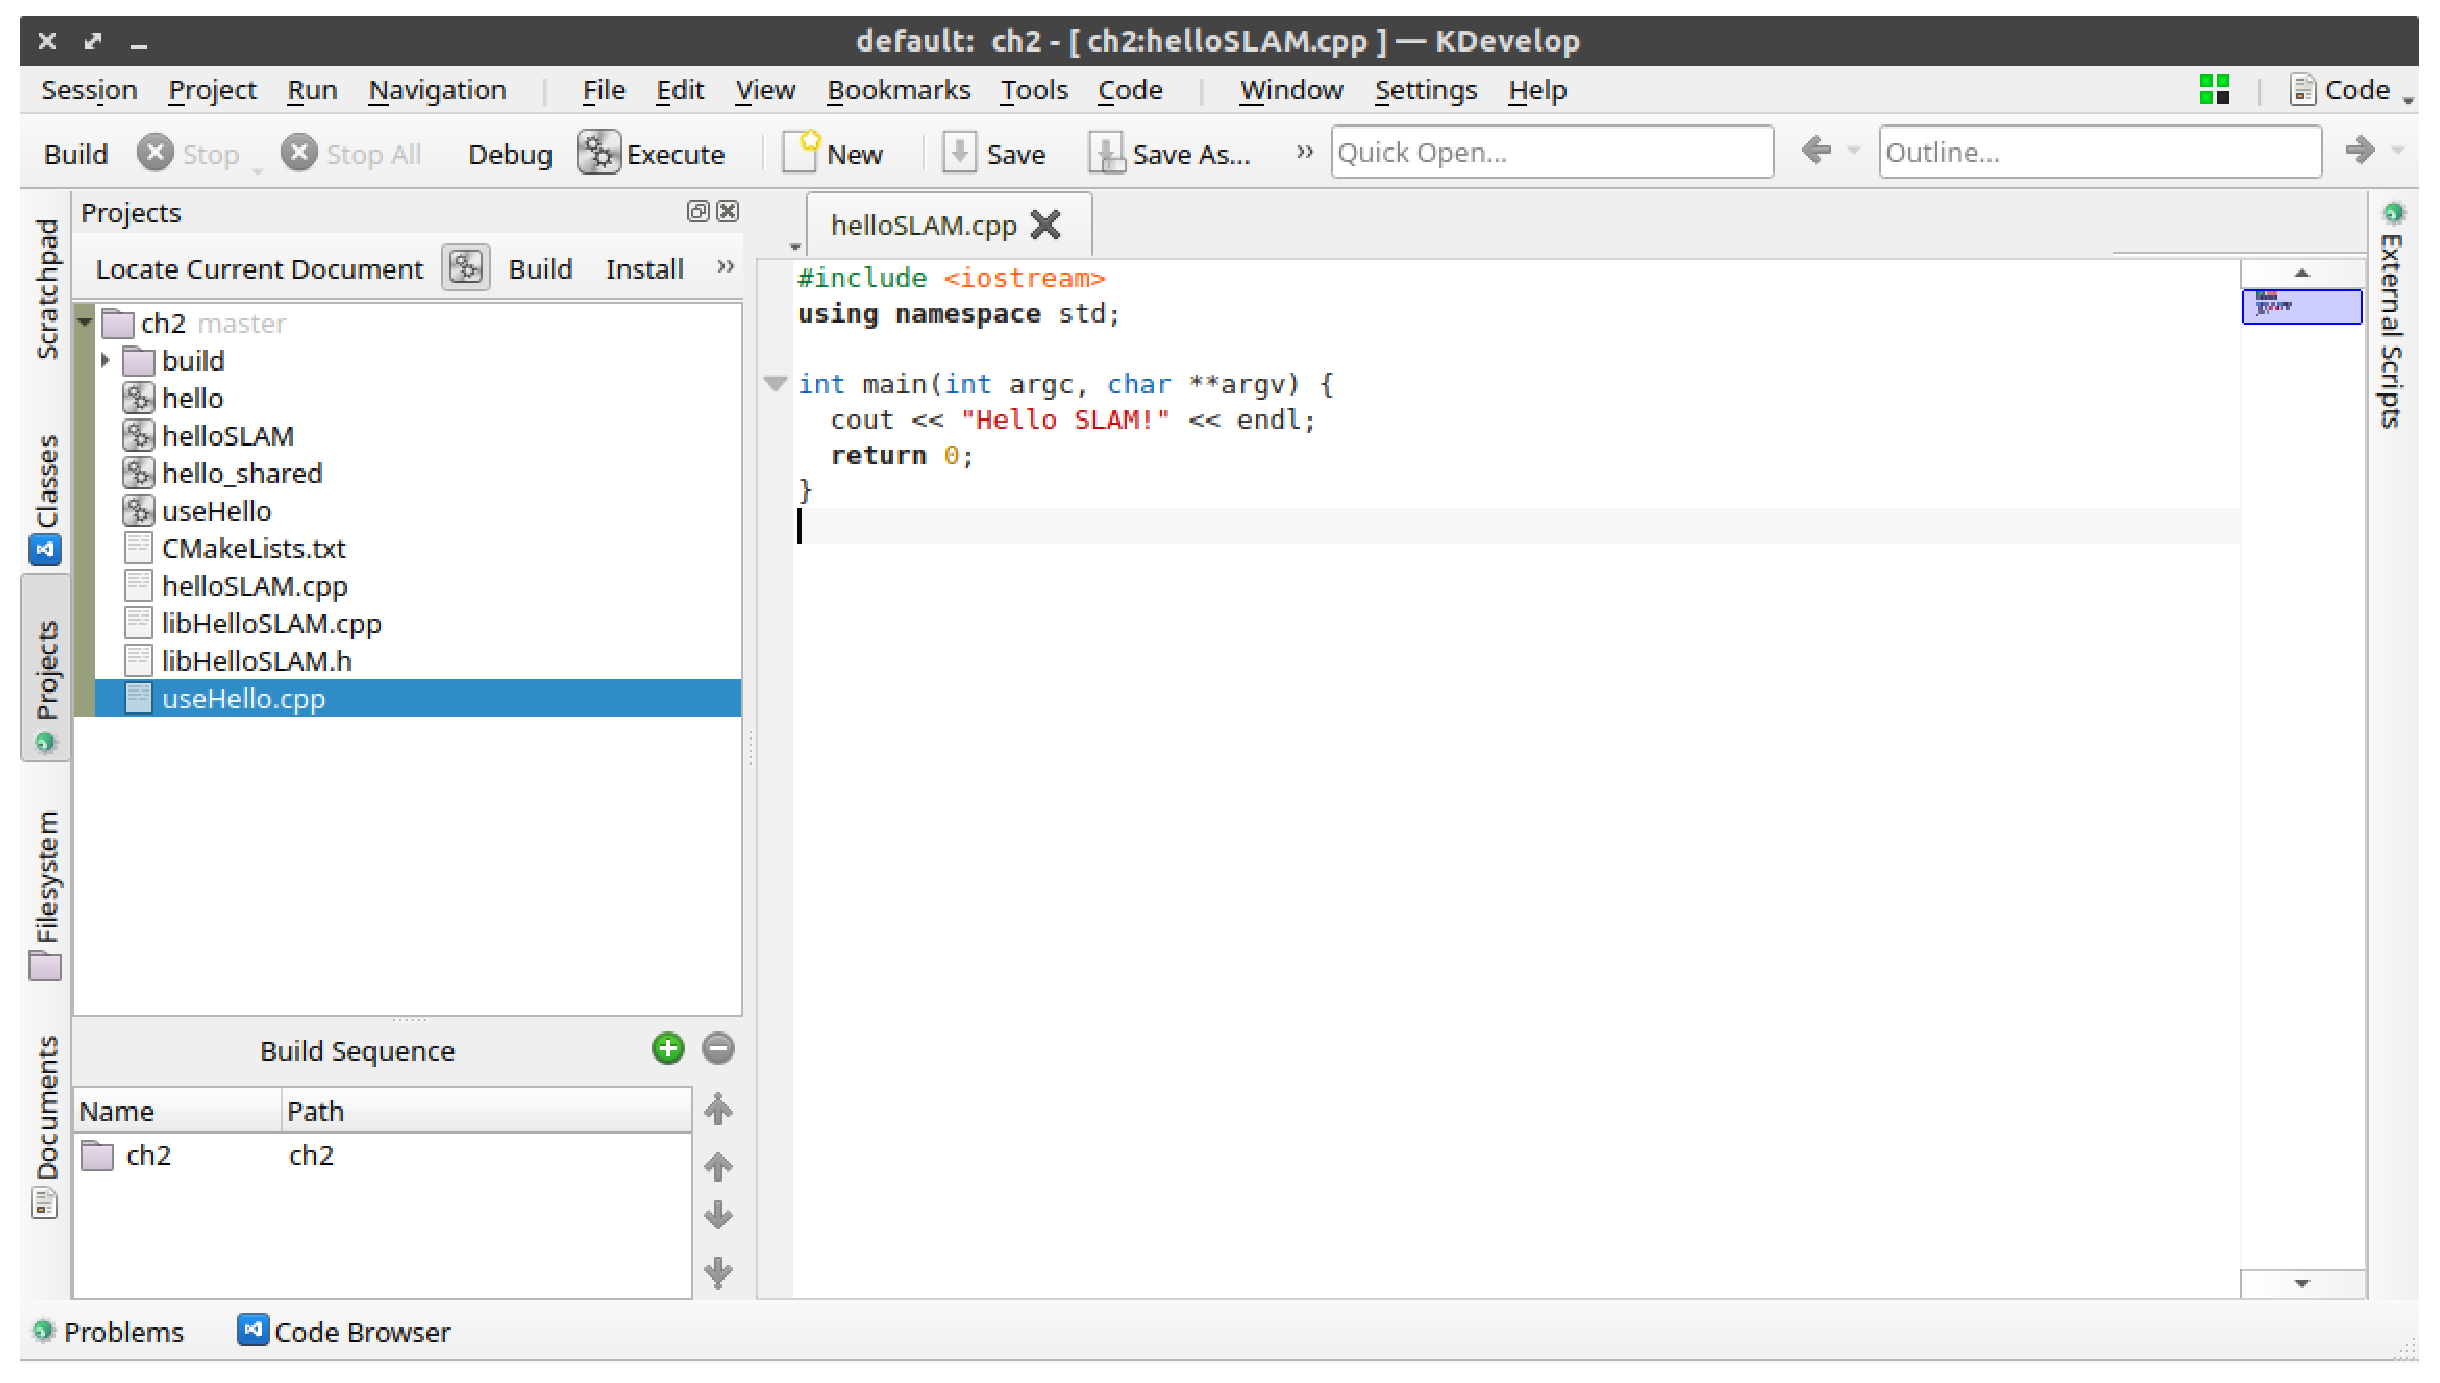
\includegraphics[width=0.8\textwidth]{whatIsSLAM/kdevelop.pdf}
    \caption{Kdevelop in Ubuntu.}
    \label{fig:kdevelop}
\end{figure}

Below we take a little bit of space to introduce KDevelop and CLion.

\subsubsection{Use KDevelop}
KDevelop natively supports the CMake project. To do this, after creating ``CMakeLists.txt'' in the terminal, open the ``CMakeLists.txt'' with ``Project $\rightarrow$Open/Import Project'' in KDevelop. The software will ask you a few questions, and by default, create a build folder to help you call the cmake and make commands. These can be done automatically by pressing the shortcut key F8. The following section of \autoref{fig:kdevelop} shows the compilation information.

We hand over the task of adapting to the IDE to the reader. If you are transferring from Windows, you will find its interface similar to Visual C++ or Visual Studio. Please use KDevelop to open the previous project and compile it to see what information it outputs. I believe you will feel more convenient than opening the terminal.

Next, let's show to debug in the IDE. Most of the students who program under Windows will have experience of breakpoint debugging under Visual Studio. However, in Linux, the default debugging tool gdb only provides a text interface, which is not convenient for novices. Some IDEs provide breakpoint debugging (the bottom layer is still gdb), and KDevelop is one of them. To use KDevelop's breakpoint debugging feature, you need to do the following:

\begin{enumerate}
    \item Set the project to Debug compilation mode in ``CMakeLists.txt'', and don't use optimization options (not used by default).
    \item Tell KDevelop which program you want to run. If there are parameters, also configure its parameters and working directory.
    \item Enter the breakpoint debugging interface, you can single step, see the value of the intermediate variable.
\end{enumerate}

%\clearpage

The first step is to set the compilation mode by adding the following command to ``CMakeLists.txt'':
\begin{lstlisting}[caption=slambook2/ch2/CMakeLists.txt]
Set( CMAKE_BUILD_TYPE "Debug" )
\end{lstlisting}

CMake has some compilation-related built-in variables that give you more precise control over the compilation process. There is usually a \textit{debug} mode for debugging and a \textit{release} mode for publishing. In debug mode, the program runs slower, but breakpoint debugging is possible, and you can see the values of the variables;. In contrast, release mode is faster, but there is probably no debugging information. We set the program to Debug mode and place the breakpoint. Next, tell KDevelop which program you want to launch.

In the second step, open ``Run $\rightarrow$Configure Launches'' and click on ``Add New $\rightarrow$ Application'' on the left. In this step, our task is to tell KDevelop which program to launch. As shown in \autoref{fig:launchConfigure}, you can either select a CMake project target (that is, the executable we built with the add\_executable directive) or point to a binary file. The second approach is recommended, and in our experience, this is less of a problem.

\begin{figure}[!ht]
    \centering
    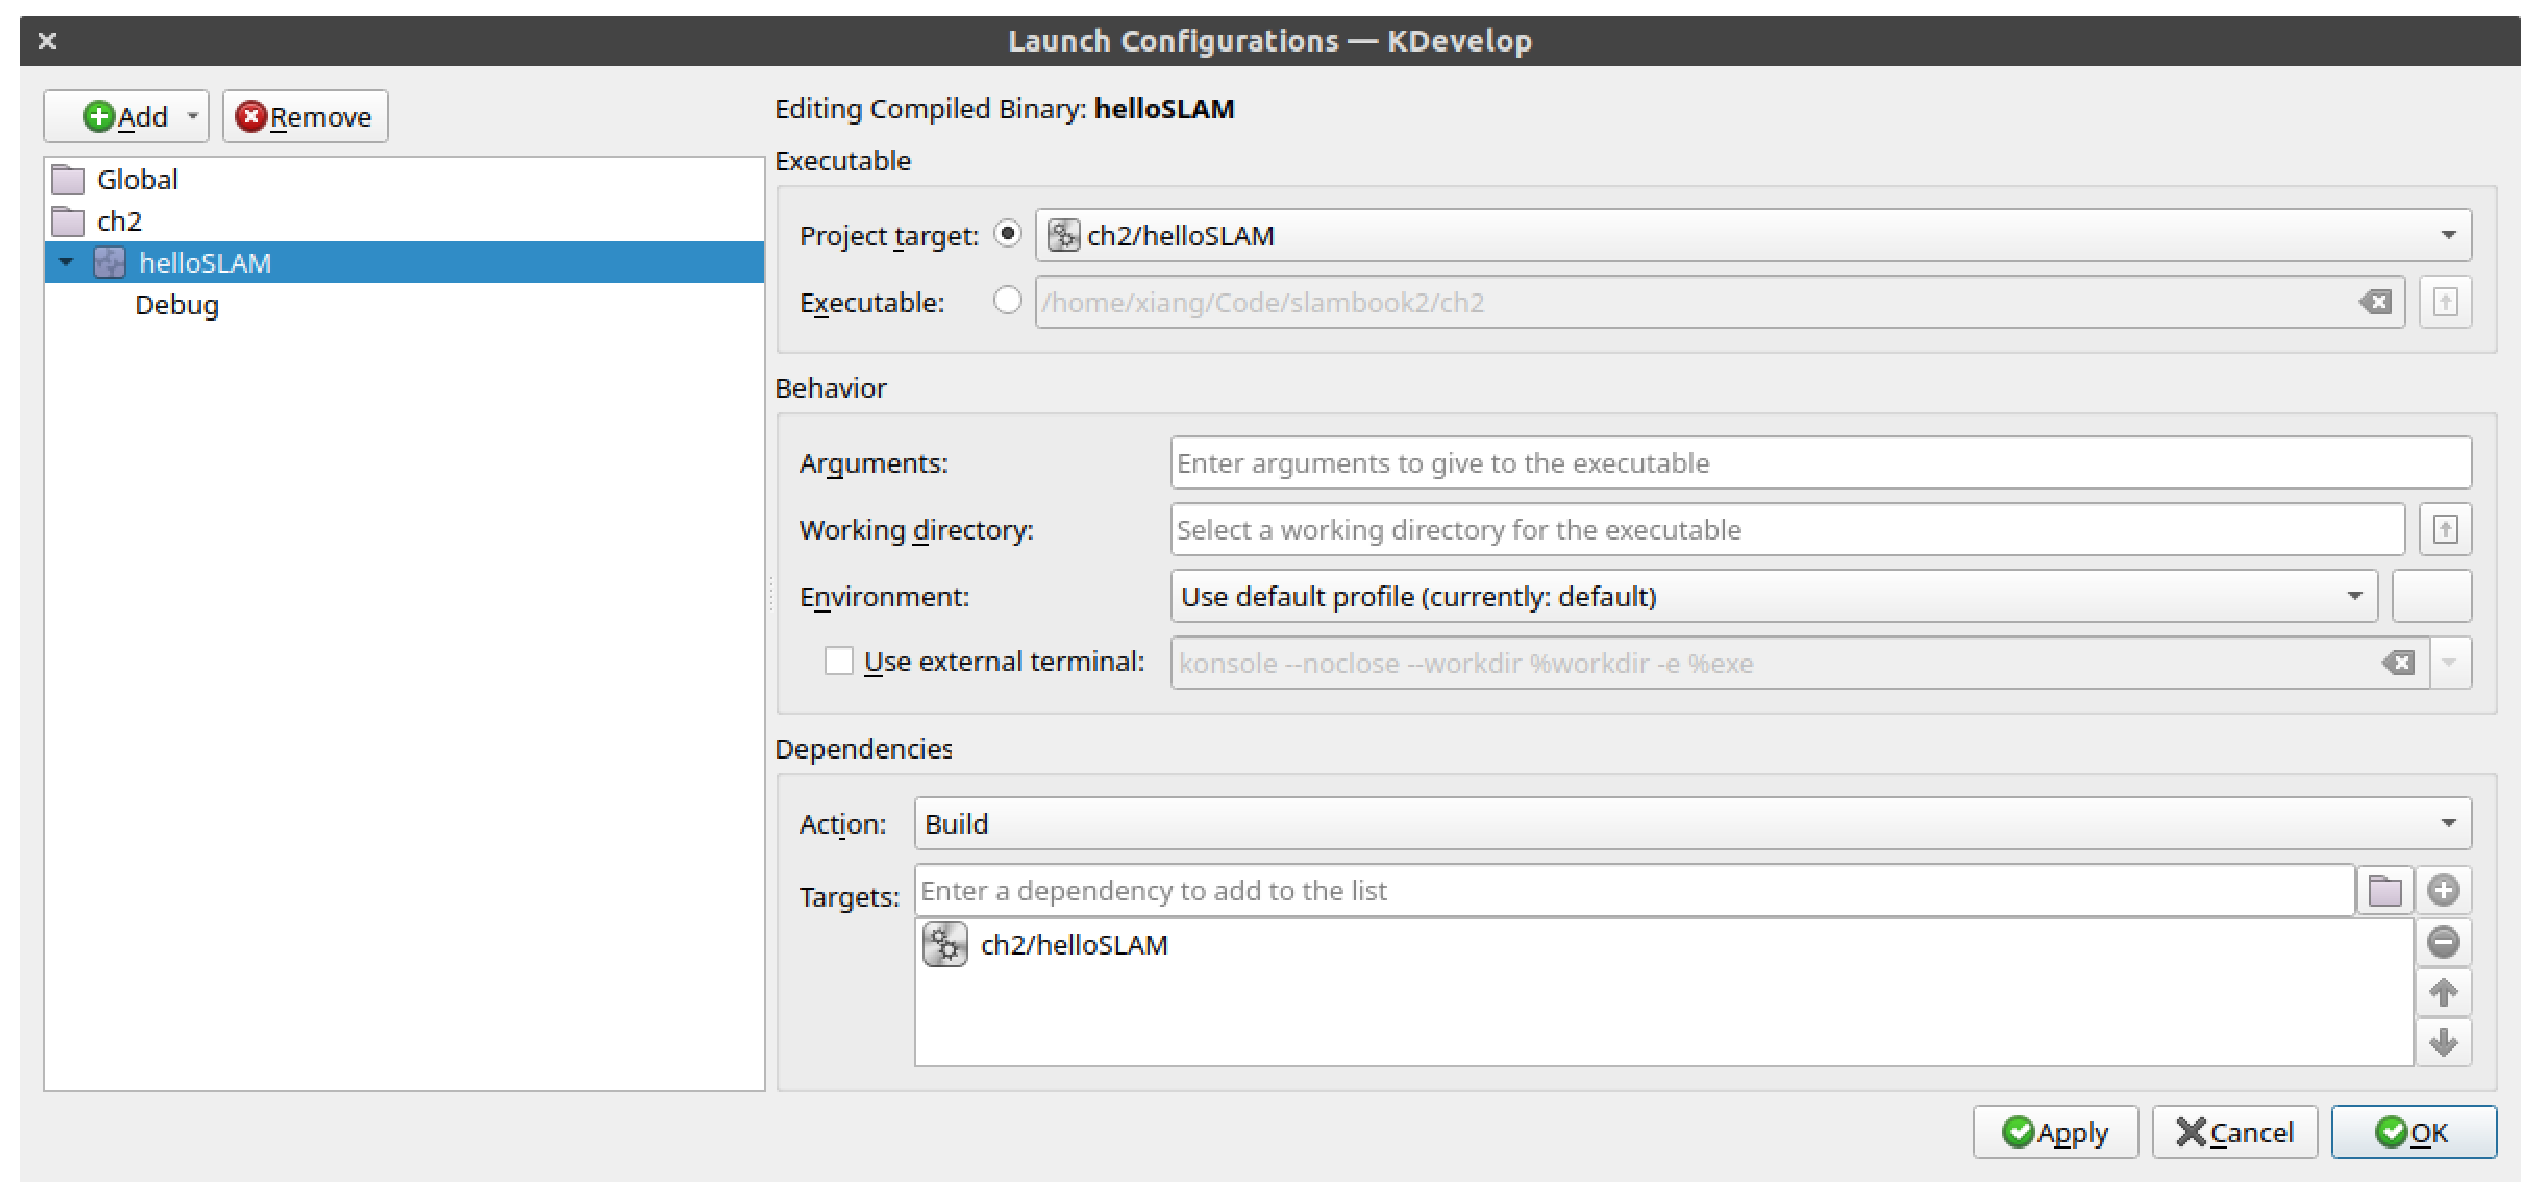
\includegraphics[width=0.8\textwidth]{whatIsSLAM/config-launch.pdf}
    \caption{Config launches. We can choose a launch target and set parameters here. }
    \label{fig:launchConfigure}
\end{figure}

In the second column, you can set the program's parameters and working directory. Sometimes programs have runtime parameters that are passed in as arguments to the main function. If not, leave it blank, as is the working directory. After configuring these two items, click the ``OK'' button to save the configuration results.

In these steps, we have configured an application launcher. We can click the ``Execute'' button to start the program directly or click the ``Debug'' button to debug it for each application. Readers can try to click the ``Execute'' button to see the results of the output. To debug this program, click on the left side of the ``printHello'' line and add a breakpoint. Then, click on the ``Debug'' button, and the program will wait at the breakpoint, as shown by \autoref{fig:debug}.

\begin{figure}[!htp]
    \centering
    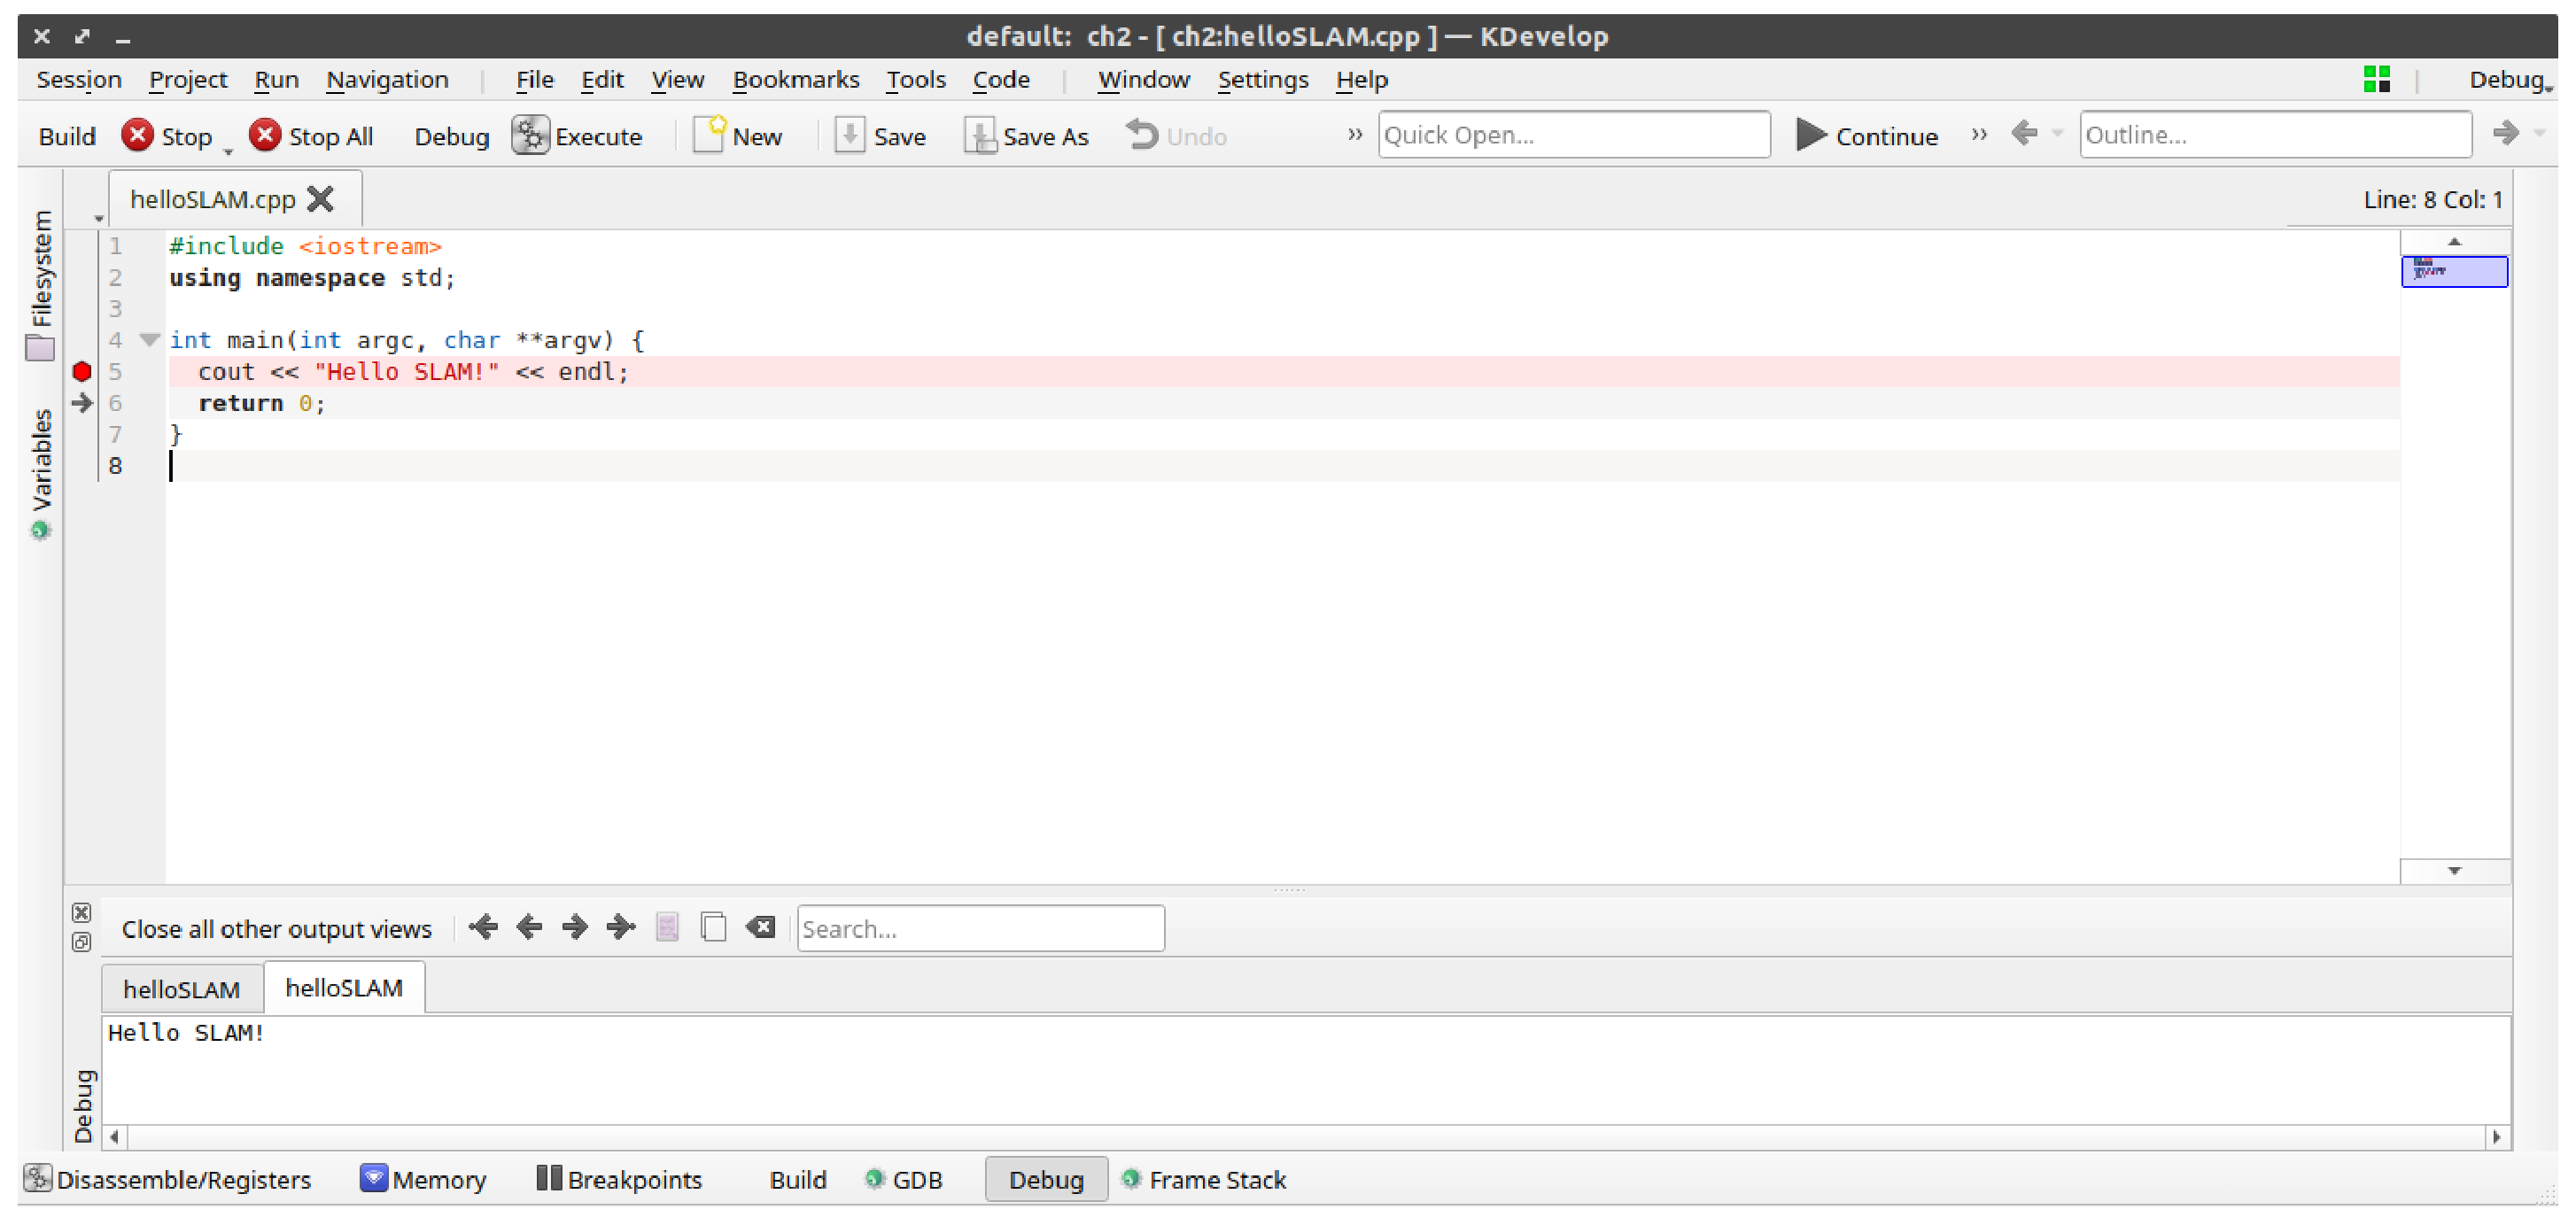
\includegraphics[width=0.8\textwidth]{whatIsSLAM/debug.pdf}
    \caption{Debug interface. }
    \label{fig:debug}
\end{figure}

When debugging, KDevelop will switch to debug mode, and the interface will change a bit. At the breakpoint, you can control the operation of the program with a single-step operation (F10 key), single-step follow up (F11 key), and single-step jump (F12 key) function. At the same time, you can click the interface on the left to view the local variable's value. Or select the ``Stop'' button to end debugging. After debugging, KDevelop will return to the normal development interface.

Now you should be familiar with the entire process of breakpoint debugging. In the future, if an error occurs during the running phase of the program, causing the program to crash, you can use breakpoint debugging to determine the location of the error, and then modify it \footnote{Instead of directly sending us an email asking how to deal with the problems. }.

\subsubsection{Use CLion}
\begin{figure}[!t]
    \centering
    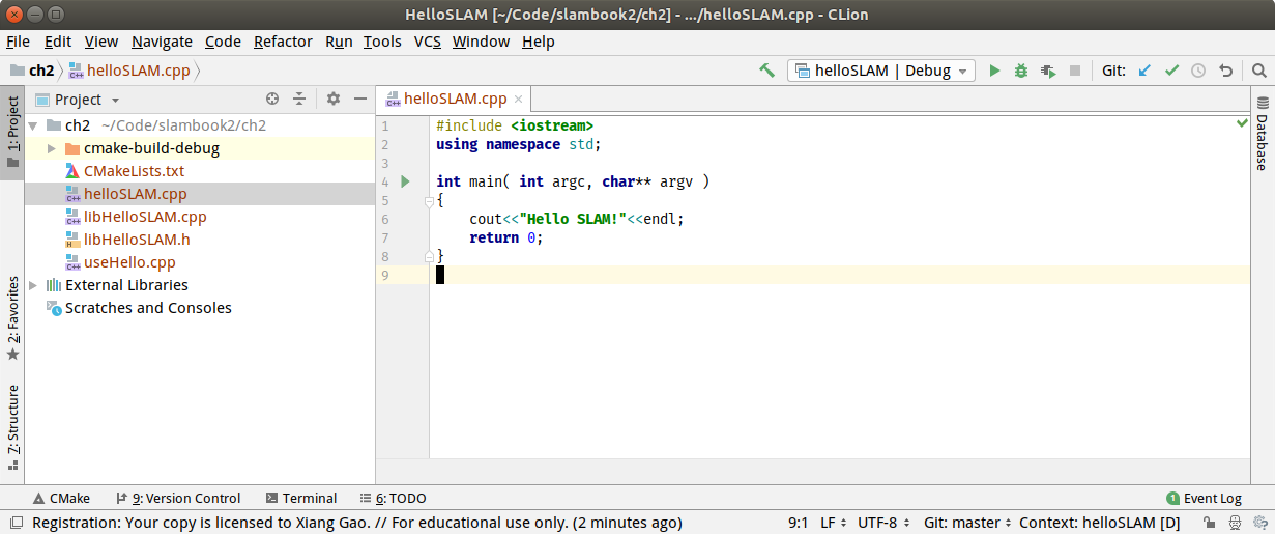
\includegraphics[width=1.0\textwidth]{whatIsSLAM/clion.pdf}
    \caption{CLion interface.}
    \label{fig:clion}
\end{figure}

CLion is more complete than KDevelop, but it requires a user account, and the memory/CPU requirements for the host will be higher. In CLion, you can also open a ``CMakeLists.txt'' or specify a directory. CLion will complete the \textit{cmake-make} process for you. Its running interface is shown in \autoref{fig:clion}.

Similarly, after opening CLion, you can select the programs you want to run or debug in the upper right corner of the interface and adjust their startup parameters and working directory. Click the small beetle button in this column to start the breakpoint debugging mode. CLion also has several convenient features, such as automatically creating classes, changing functions, and automatically adjusting the coding style. Please try it.

OK, if you are already familiar with the IDE's usage, then the second chapter will stop here. You may already feel that I have talked too much, so in the following practice section, we will not introduce things like creating a new build folder, calling the \textit{cmake} and \textit{make} commands to compile the program. I believe that readers should master these simple steps. Similarly, since most of the third-party libraries used in this book are cmake projects, you will continue to be familiar with the compilation process. Next, we will start the formal chapter and introduce some related mathematics.

\section*{Exercises}
\begin{enumerate}
    \item[\optional] Read SLAM's review literature, such as~\cite{Cadena2016, Fuentes-Pacheco2015, Boal2014, Chen2012, Chen2007} and so on. What are the similarities and differences between these papers on SLAM and this book?
    \item What are the parameters of the g++ command? If I want to change the generated program file name, how should I call g++?
    \item Use the build folder to compile your CMake project, then try it in KDevelop.
    \item Deliberately add some syntax errors to the code to see what information the build will generate. Can you read the error message of g++?
    \item If you forgot to link the library to the executable, will the compiler report an error? What kind of mistakes are reported?
    \item[\optional] Read ``CMake practice'' (or other materials) to learn about the grammars of CMake.
    \item[\optional] Improve the hello SLAM problem, make it a small library, and install it on your local hard drive. Then, create a new project, use find\_package to find the library, and call it.
    \item[\optional] Read other CMake instructional materials, such as \url{https://github.com/TheErk/CMake-tutorial}.
    \item Find the official website of KDevelop and see what other features it has. Are you using it?
    \item If you learned vim in the last lecture, please try KDevelop's/CLion's vim editing function.
\end{enumerate}
% !Mode:: "TeX:UTF-8"
\chapter{3D Rigid Body Motion}
\label{cpt:3}

\begin{mdframed}
	\textbf{Goal of Study}
	\begin{enumerate}
		\item Study the rigid body geometry in three-dimensional space: rotation matrix, transformation matrix, quaternion, and Euler angle.
		\item Learn the usage of the \textit{Eigen} library's matrix and geometry module.
	\end{enumerate}
\end{mdframed}

In the last lecture, we explained the framework and content of visual SLAM. This lecture will introduce one of the fundamental problems of visual SLAM: How to describe a rigid body's motion in three-dimensional space? Intuitively, we certainly know that this consists of one rotation plus one translation. The translation part does not really have any problems, but the rotation part is questionable. We will introduce the meaning of rotation matrices, quaternions, Euler angles and how they are computed and transformed. In the practice section, we will introduce one of the widely used linear algebra libraries: \textit{Eigen}. It provides a C++ matrix calculation, and its geometry module also provides the necessary data structures and operations, like quaternions. \textit{Eigen} is heavily optimized, but there are still some special issues to be discussed about its usage. We will leave it to the practice part.

\newpage
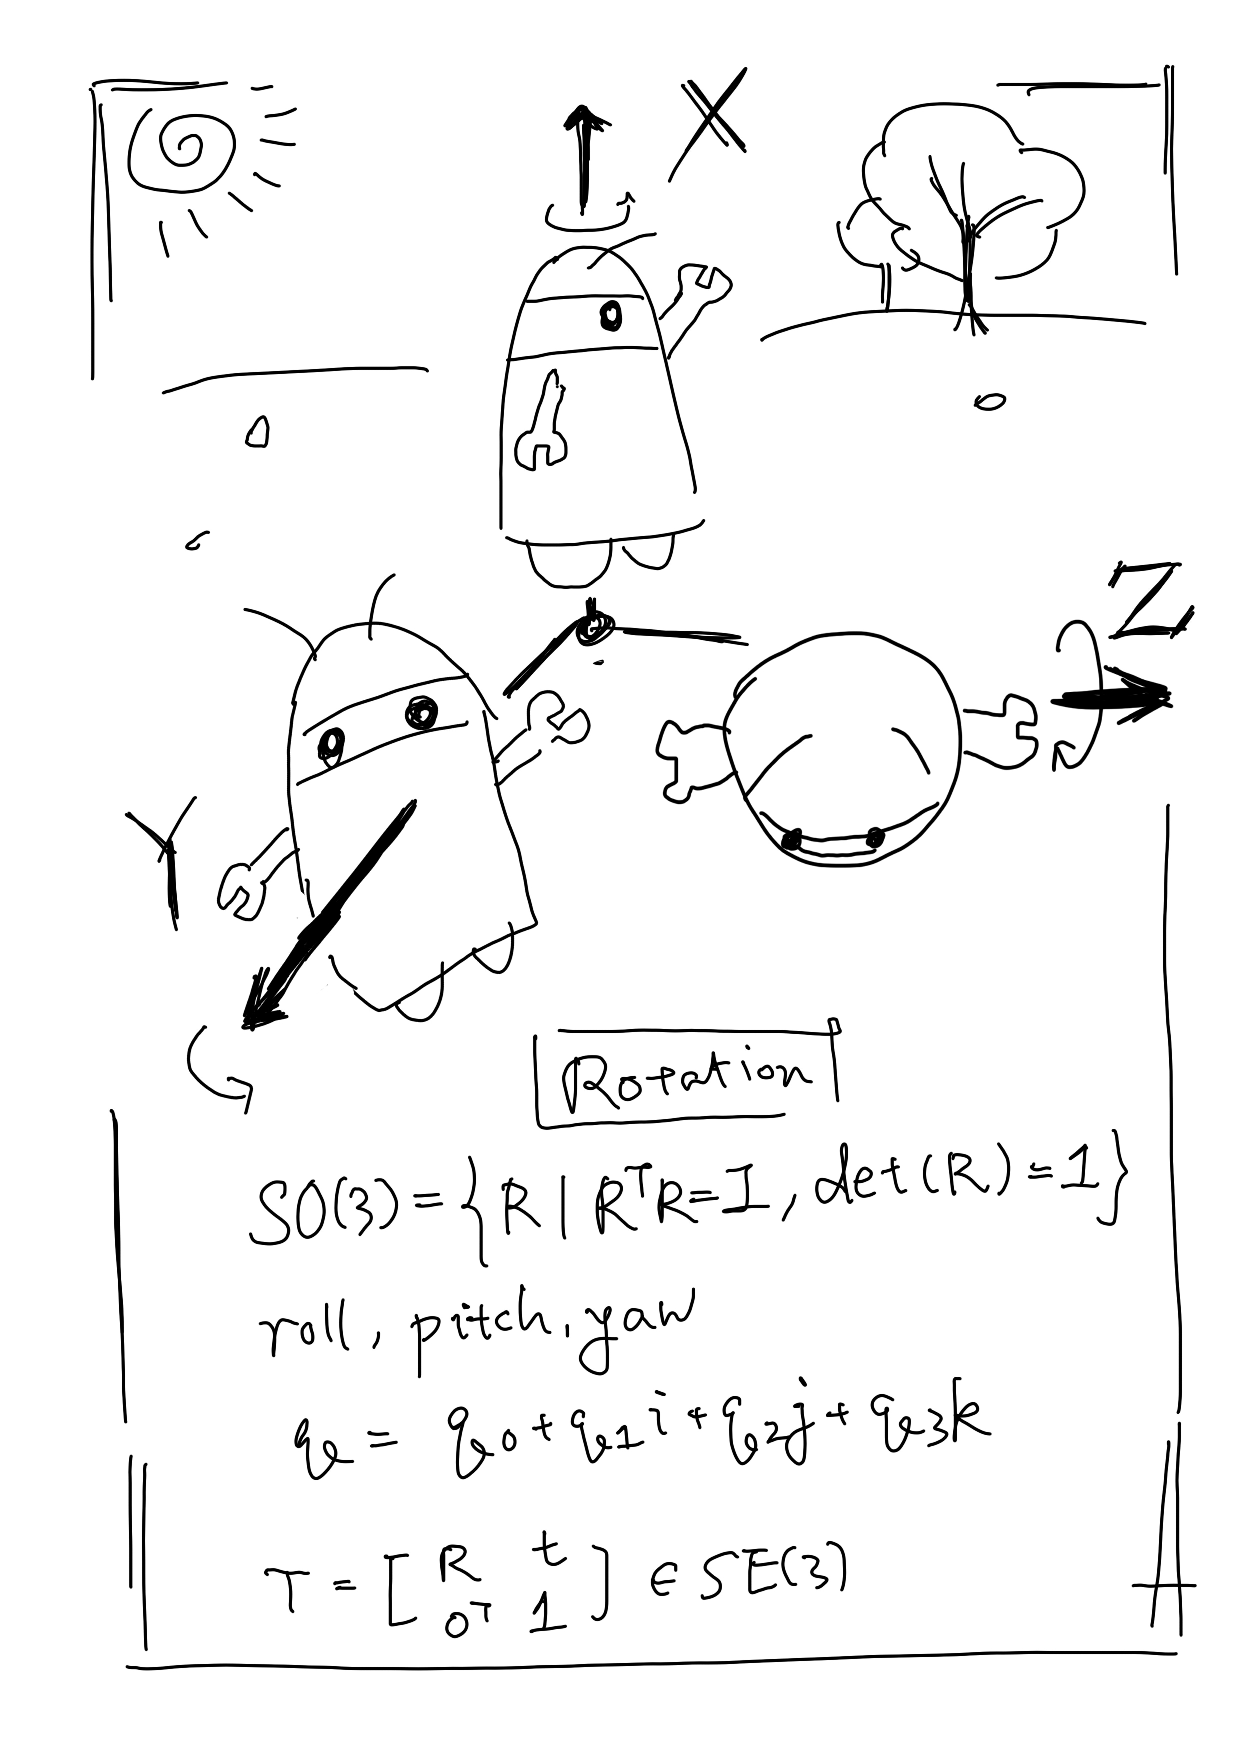
\includepdf{resources/other/ch3.pdf}
\newpage

\section{Rotation Matrix}
\label{sec:3.1}
\subsection{Points, Vectors, and Coordinate Systems}
The space of our daily life is three-dimensional, so we are born to be used to 3D movements. The 3D space consists of three axes, so the position of one spatial point can be specified by three coordinates. However, we should now consider a rigid body, which has its \textit{position} and \textit{orientation}. The camera can also be viewed as a rigid body in three dimensions, so what we care about in VSLAM are the problem of the camera's position and orientation.  Combined, we can say, ``the camera is at the $( 0, 0, 0)$ point, facing the front''. But this natural language is troublesome, and we prefer to describe it in a mathematical language.

We start from the most basic content: \textit{points} and \textit{vectors}. Points are the basic elements in space, no length, no volume. Connecting the two points forms a vector. A vector can be thought of as an arrow pointing from one point to another. Here we need to remind the reader that please do not confuse the vector with its coordinates. A vector is one thing in space, such as $ \mathbf{a}$. Here $ \mathbf{a} $ does not need to be associated with several real numbers. We can naturally talk about the plus or minus operation of two vectors, without relating to any real numbers. Only when we specify a coordinate system in this 3D space can we talk about the vector's coordinates in this system, finding several real numbers corresponding to this vector.

With the knowledge of linear algebra, the coordinates of a point in 3D space can be described by $ \mathbb{R}^3$. How to describe it? Suppose that in this linear space, we find a set of base \footnote{Just a reminder here, the base is a set of linearly independent vectors in the space, normally being orthogonal and has unit-length.} $ (\mathbf{e}_1,\mathbf{e}_2,\mathbf{e}_3) $, then, an arbitrary vector $ \mathbf{a} $ has a \textit{coordinate} under this base:
\begin{equation}
\mathbf{a} = \left[ {{\mathbf{e}_1},{\mathbf{e}_2},{\mathbf{e}_3}} \right]\left[ \begin{array}{l}
{a_1}\\
{a_2}\\
{a_3}
\end{array} \right] = {a_1}{\mathbf{e}_1} + {a_2}{\mathbf{e}_2} + {a_3}{\mathbf{e}_3}.
\end{equation}

Here $ (a_ 1, a_ 2, a_ 3 )^{T} $ is called $\mathbf {a}$'s coordinates \footnote {We use column vectors in this book which is same as most of the  mathematics books.}. The coordinates' specific values are related to the vector itself and the selection of the bases. In $\mathbb{R}^3$, the coordinate system usually consists of 3 orthogonal coordinate axes (it can also be non-orthogonal, but it is rare in practice). For example, given $ \mathbf {x} $ and $ \mathbf {y} $ axis, the $ \mathbf {z} $ axis can be determined using the right-hand (or left-hand) rule by $ \mathbf {x} \times  \mathbf {y} $. According to different definitions, the coordinate system is divided into left-handed and right-handed. The third axis of the left-hand rule is opposite to the right-hand rule. Most 3D libraries use right-handed coordinates (such as OpenGL, 3DS Max, etc.), and some libraries use left-handed coordinates (such as Unity, Direct3D, etc.).

Based on basic linear algebra knowledge, we can talk about the operations between vectors/vectors, vectors/numbers, such as scalar multiplication, vector addition, subtraction, inner product, outer product, and so on. Multiplication, addition, and subtraction are fairly basic and intuitive. For example, the result of adding two vectors is to add their respective coordinates, and the same for subtraction, and so on. I won't go into details here. Inner and outer products may be somewhat unfamiliar to the reader, and their calculations are given here. For $ \mathbf {a}, \mathbf {b} \in  \mathbb {R}^ 3 $, in the common definition \footnote {The inner product also has more general definitions, but this book only discusses the usual inner product.}, the inner product of $\mathbf{a}, \mathbf{b}$ can be written as:

\begin{equation}
\mathbf{a} \cdot \mathbf{b} = { \mathbf{a}^T }\mathbf{b} = \sum\limits_{i = 1}^3 {{a_i}{b_i}}  = \left| \mathbf{a} \right|\left| \mathbf{b} \right|\cos \left\langle {\mathbf{a},\mathbf{b}} \right\rangle ,
\end{equation}
where $ \left \langle { \mathbf {a}, \mathbf {b}} \right \rangle $ refers to the angle between the vector $ \mathbf {a}, \mathbf {b} $. The inner product can also describe the projection relationship between vectors. The outer product is like this:

\begin{equation}
\label{eq:cross}
\mathbf{a} \times \mathbf{b} = \left\| {\begin{array}{*{20}{c}}
	\mathbf{e}_1 & \mathbf{e}_2 & \mathbf{e}_3 \\
	{{a_1}}&{{a_2}}&{{a_3}}\\
	{{b_1}}&{{b_2}}&{{b_3}}
	\end{array}} \right\| = \left[ \begin{array}{l}
{a_2}{b_3} - {a_3}{b_2}\\
{a_3}{b_1} - {a_1}{b_3}\\
{a_1}{b_2} - {a_2}{b_1}
\end{array} \right] = \left[ {\begin{array}{*{20}{c}}
	0&{ - {a_3}}&{{a_2}}\\
	{{a_3}}&0&{-{a_1}}\\  
	{-{a_2}}&{{a_1}}&0  
	\end{array}} \right] \mathbf{b} \buildrel \Delta \over = { \mathbf{a}^ \wedge } \mathbf{b}.
\end{equation}

The result of the outer product is a vector whose direction is perpendicular to the two vectors, and the length is $ \left | \mathbf{a} \right | \left | \mathbf{b} \right | \left \langle { \mathbf {a}, \mathbf {b}} \right \rangle  $, which is also the area of the quadrilateral of the two vectors. From the outer product operations, we introduce the $ ^ \wedge $ operator here, which means writing $ \mathbf{a} $ as a \textit {skew-symmetric matrix} \footnote{Skew-symmetric matrix means $ \mathbf{A} $ satisfies $ \mathbf{A}^T=- \mathbf{A}$. }. You can take $ ^ \wedge $ as a skew-symmetric symbol. It turns the outer product $ \mathbf{a} \times  \mathbf{b} $ into the multiplication of the matrix and the vector $ { \mathbf{a}^ \wedge } \mathbf{b} $, which is a linear operatoration. This symbol will be used frequently in the following sections. This symbol will be used frequently in the following sections. It is a one-to-one mapping, meaning that for any vector, it corresponds to a unique anti-symmetric matrix, and vice versa:

\begin{equation}
\mathbf{a}^\wedge = \left[ {\begin{array}{*{20}{c}}
	0&{-{a_3}}&{{a_2}}\\  
	{{a_3}}&0&{ - {a_1}}\\
	{ - {a_2}}&{{a_1}}&0
	\end{array}} \right].
\end{equation}

At the same time, note that the vector operations such as addition, subtraction, inner and outer products can be calculated even when we do not have their coordinates. For example, although the inner product can be expressed by the sum of the two vectors' product when we know the coordinates, the length and angle can also be calculated even if their coordinates are unknown. Therefore, the inner product result of the two vectors is independent of the selection of the coordinate system.

\subsection{Euclidean Transforms Between Coordinate Systems}
We often define a variety of coordinate systems in the real scene. In robotics, you define one coordinate system for each link and joint; in 3D mapping, we also define a coordinate system for each cuboid and cylinder. If we consider a moving robot, it is common practice to set a stationary inertial coordinate system (or world coordinate system), such as the $x_W, y_W, z_W$ defined in Fig.~\ref{fig:axisTransform}. Meanwhile, the camera or robot is a moving coordinate system, such as the coordinate system defined by $x_C, y_C, z_C$. We might ask: a vector $\mathbf{p}$ in the camera system may have coordinates $\mathbf{p}_c$; and in the world coordinate system, its coordinates maybe $ \mathbf{p}_w$. Then what is the conversion between these two coordinates? It is necessary to first obtain the coordinate values of the point in the camera system and then use the transform rule to do the coordinate transform. We need a mathematical way to describe this transformation. As we will see later, we can describe it with a transform matrix $\mathbf{T}$.

\begin{figure}[!htp]
    \centering
    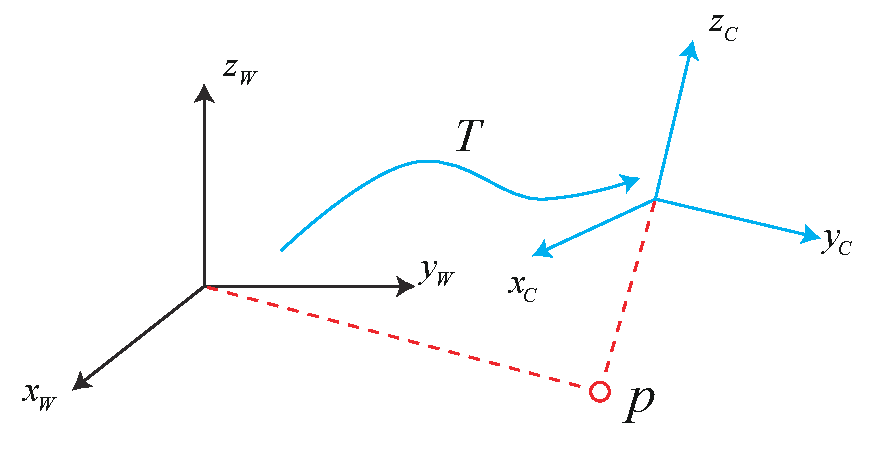
\includegraphics[width=0.7\textwidth]{rigidMotion/axisTransform.pdf}
    \caption {Coordinate transform. For the same vector $ \mathbf{p}$, its coordinates in the world $\mathbf{p}_W$ and the coordinates in the camera system $ \mathbf{p}_C$ are different. This transformation relationship is described by the transform matrix $ \mathbf{T} $.}
    \label{fig:axisTransform}
\end{figure}

Intuitively, the motion between two coordinate systems consists of a rotation plus a translation, which is called \textit{rigid body motion}. Obviously, the camera movement is rigid. During the rigid body motion, the length and angle of the vector will not change. Imagine you throw your phone into the air and \footnote {Please don't put it into practice because you may regret doing that.}, there may only be differences in spatial position and orientation. But the length and the angle of each face will not change. The phone will not be squashed like an eraser or be stretched during this motion. At this point, we say that the phone's motion is  \textit {Euclidean}.

The Euclidean transform consists of rotation and translation. Let's first consider the rotation. We have a unit-length orthogonal base $ ( \mathbf {e}_ 1, \mathbf {e}_ 2, \mathbf {e}_ 3 ) $. After a rotation it becomes $ ( \mathbf {e}_ 1 ', \mathbf {e}_ 2 ', \mathbf {e}_ 3 ') $. Then, for the same vector $ \mathbf {a} $ (the vector does not move with the rotation of the coordinate system), its coordinates in these two coordinate systems are $ [a_ 1, a_ 2, a_ 3 ] ^ \mathrm {T} $ and $[a'_ 1, a'_ 2, a'_ 3 ]^ \mathrm {T} $. Because the vector itself has not changed, according to the definition of coordinates, there are:

\begin{equation}
\left[ \mathbf{e}_1,\mathbf{e}_2,\mathbf{e}_3 \right]\left[ \begin{array}{l}
{a_1}\\
{a_2}\\
{a_3}
\end{array} \right] = \left[ \mathbf{e}_1', \mathbf{e}_2', \mathbf{e}_3' \right]\left[ \begin{array}{l}
a'_1\\
a'_2\\
a'_3
\end{array} \right].
\end{equation}

To describe the relationship between the two coordinates, we multiply the left and right sides of the above equation by $ \left [ \begin {array}{l}
\mathbf{e}_1^T\\
\mathbf{e}_2^T\\
\mathbf{e}_3^T
\end {array} \right ] $, then the matrix on the left becomes an identity matrix, so:

\begin{equation}
\left[ \begin{array}{l}
{a_1}\\
{a_2}\\
{a_3}
\end{array}\right]=\underbrace{\left[{\begin{array}{*{20}{c}}    
    {\mathbf{e}_1^T\mathbf{e}_1'} & {\mathbf{e}_1^T\mathbf{e}_2'} & {\mathbf{e}_1^T\mathbf{e}_3'}\\
    {\mathbf{e}_2^T\mathbf{e}_1'} & {\mathbf{e}_2^T\mathbf{e}_2'} & {\mathbf{e}_2^T\mathbf{e}_3'}\\
    {\mathbf{e}_3^T\mathbf{e}_1'} & {\mathbf{e}_3^T\mathbf{e}_2'} & {\mathbf{e}_3^T\mathbf{e}_3'}
    \end{array}} \right]}_{\text{rotation matrix}}\left[ \begin{array}{l}
a_1'\\
a_2'\\
a_3'
\end{array} \right] \buildrel \Delta \over = \mathbf{R} \mathbf{a}'.
\end{equation}
We take the intermediate matrix out and define it as a matrix $ \mathbf{R}$. This matrix consists of the inner product between the two sets of bases, describing the same vector's coordinate transformation relationship before and after the rotation. As long as the rotation is the same, this matrix is the same. It can be said that the matrix $ \mathbf{R} $ describes the rotation itself. So we call it the \textit{rotation matrix}. Meanwhile, the components of the matrix are the inner product of the two coordinate system bases. Since the base vector's length is 1, it is actually the cosine of the angle between the base vectors. So this matrix is also called \textit{direction cosine matrix}. We will just call it the rotation matrix in the following.

The rotation matrix has some special properties. In fact, it is an \textit{orthogonal} matrix with a determinant of 1 \footnote{Orthogonal matrix is a matrix whose inverse is its transpose. The orthogonality of the rotation matrix can be derived directly from the definition. } \footnote{The determinant is 1 is artificially defined. In fact, its determinant is $\pm 1 $, but the rotation with determinant $ - 1 $ is called \textit{improper rotation}, that is, one rotation plus one reflection in 3D space. }. Conversely, an orthogonal matrix with a determinant of 1 is also a rotation matrix. So, you can define a set of $n$ dimensional rotation matrices as follows:
\begin{equation}
\mathrm{SO}(n) = \{ \mathbf{R} \in \mathbb{R}^{n \times n} | \mathbf{R R}^T = \mathbf{I}, \mathrm{det} (\mathbf{R})=1 \}.
\end{equation}

$\mathrm{SO}(n) $ refers to the \textit {special orthogonal group}. We leave the contents of the ``group'' to the next lecture. This set consists of a rotation matrix of $ n $ dimensional space, in particular, $\mathrm {SO}(3)$ refers to the rotation of the three-dimensional space. In this way, we can talk directly about the rotation transformation between the two coordinate systems without having to start from the bases.

Since the rotation matrix is orthogonal, its inverse (i.e., transpose) describes an opposite rotation. According to the above definition, there are:
\begin{equation}
\mathbf{a} '= \mathbf{R}^{-1} \mathbf{a} = \mathbf{R}^{T} \mathbf{a}.
\end{equation}
Obviously the $ \mathbf{R}^T $ represents an opposite rotation.

In the Euclidean transformation, there is a translation in addition to the rotation. Consider the vector $ \mathbf{a} $ in the world coordinate system, after a rotation (depicted by $ \mathbf{R} $) and a translation of $ \mathbf{t} $, we get $ \mathbf{a}' $. Then we can put the rotation and translation together, and have:
\begin{equation}
\label{eq:RT}
\mathbf{a} '= \mathbf{R} \mathbf{a} + \mathbf{t},
\end{equation}
where $ \mathbf{t} $ is called a translation vector. Compared to the rotation, the translation part simply adds the translation vector to the coordinates after the rotation, which is very simple. By the above formula, we completely describe the coordinate transformation relationship using a rotation matrix $ \mathbf{R} $ and a translation vector $ \mathbf{t}$. In practice, we may define the coordinate system 1 and 2, then the vector $ \mathbf{a} $ under the two coordinates is $ \mathbf{a}_1, \mathbf{a}_2 $. The relationship between the two systems should be:
\begin{equation}
\mathbf{a}_1 = \mathbf{R}_{12} \mathbf{a}_2 + \mathbf{t}_{12}.
\end{equation}
Here $ \mathbf{R}_{12} $ means ``rotation of the vector from system 2 to system 1''. Since the vector is multiplied to the right of the rotation matrix, its subscript is \textit{read from right to left}. This is just a customary way of writing this book. Coordinate transformations are easy to confuse, especially if multiple coordinate systems exist. Similarly, if we want to express ``rotation matrix from 1 to 2'', we write it as $ \mathbf{R}_{21}$. The reader must be clear about the notation here, because different books may have different notations. Some notations about rotation will be denoted as the top left/subscript, and the text will be written on the right side.

About $\mathbf{t}_{12}$, readers may just take it as a translation vector without wondering about its physical meaning. In fact, it corresponds to a vector from the system 1's origin pointing to system 2's origin, and the coordinates are taken under system 1. So I suggest readers understand it as ``a vector from 1 to 2''. But the reverse $ \mathbf{t}_{21} $, which is a vector from 2's origin to 1's origin, whose \textit{coordinates are taken in system 2}, is not equal to $-\mathbf{t}_{12}$. It is also related to the rotation of the two systems. \footnote{Although they are indeed inverse relations from the vector level, the coordinates of the two vectors are not the opposite. Can you find out why it looks like this?} Therefore, when beginners ask the question ``What are my coordinates?'', we need to clearly explain this sentence's meaning. Here ``my coordinates'' normally refers to the vector from the world system $W$ pointing to the origin of the camera system $C$, and then take the coordinates in the world's base. Corresponding to the mathematical symbol, it should be the value of $ \mathbf{t}_{WC} $. For the same reason, it is not $ - \mathbf {t}_{CW}$, but actually $-\mathbf{R}_{CW}^T \mathbf{t}_{CW}$.

\subsection{Transform Matrix and Homogeneous Coordinates}
The formula~\eqref{eq:RT} fully expresses the rotation and translation of Euclidean space, but there is still a small problem: the transformation relationship here is not a linear relationship. Suppose we made two transformations: $ \mathbf {R}_ 1, \mathbf {t}_ 1 $ and $ \mathbf {R}_ 2, \mathbf {t}_ 2 $:
\[
\mathbf{b} = {\mathbf{R}_1} \mathbf{a} + {\mathbf{t}_1}, \quad \mathbf{c} = {\mathbf{R}_2} \mathbf{b} + {\mathbf{t}_2}.
\]
So, the transformation from $ \mathbf{a} $ to $ \mathbf{c} $ is:
\[
\mathbf{c} = {\mathbf{R}_2}\left( {{\mathbf{R}_1} \mathbf{a} + {\mathbf{t}_1}} \right) + {\mathbf{t}_2}.
\]
This form is not elegant after multiple transformations. Therefore, we introduce homogeneous coordinates and transformation matrices, rewriting the form~\eqref{eq:RT}:
\begin{equation}
\left[\begin{array}{l} 
\mathbf {a} ' \\
1
\end{array} \right] = 
\left[ {\begin{array}{*{20}{c}}
    \mathbf{R}&\mathbf{t}\\
    {{\mathbf{0}^T}}&1
    \end{array}} \right]
\left[ \begin{array}{l}
\mathbf {a} \\
1
\end{array} \right]  \buildrel \Delta \over = \mathbf{T} \left[ \begin{array}{l}
\mathbf {a} \\
1
\end{array} \right].
\end{equation}

This is a mathematical trick: we add $ 1 $ at the end of a 3D vector and turn it into a 4D vector called \textit{homogeneous coordinates}. For this four-dimensional vector, we can write the rotation and translation in one matrix, making the whole relationship a linear relationship. In this formula, the matrix $ \mathbf {T} $ is called \textit{transform matrix}.

We temporarily use $  \tilde { \mathbf {a} } $ to represent the homogeneous coordinates of $ \mathbf {a} $. Then, relying on homogeneous coordinates and transformation matrices, the superposition of the two transformations can have a good form:
\begin{equation}
\tilde{\mathbf{b}} = \mathbf{T}_1 \tilde{\mathbf{a}}, \  \tilde{\mathbf{c}} = \mathbf{T}_2 \tilde{\mathbf{b}} \quad \Rightarrow \tilde{\mathbf{c}} = \mathbf{T}_2 \mathbf{T_1} \tilde{\mathbf{a}}.
\end{equation}
But the symbols that distinguish between homogeneous and non-homogeneous coordinates are annoying, because here we only need to add 1 at the end of the vector or remove 1 to turn it into a normal vector \footnote {But the purpose of the homogeneous coordinates is not limited to this, we will come back to it in chapter \ref{cpt:7}.}. So, without ambiguity, we will write it directly as $ \mathbf {b}= \mathbf {T} \mathbf {a} $, and by default we just assume a homogeneous coordinate conversion is made if needed \footnote { Note that if homogeneous coordinate transformation is not performed, the matrix multiplication here does not make sense. }.

The transformation matrix $\mathbf{T}$ has a special structure: the upper left corner is the rotation matrix, the right side is the translation vector, the lower-left corner is $ \mathbf{0} $ vector, and the lower right corner is 1. This set of transform matrix is also known as the \textit{special Euclidean group}:

\begin{equation}
\mathrm{SE}(3) = \left\{ \mathbf{T} = \left[ {\begin{array}{*{20}{c}}
    \mathbf{R} & \mathbf{t} \\
    {{\mathbf{0}^T}} & 1
    \end{array}} \right]
\in \mathbb{R}^{4 \times 4} | \mathbf{R} \in \mathrm{SO}(3), \mathbf{t} \in \mathbb{R}^3\right\} .
\end{equation}

Like $ \mathrm{SO}( 3 ) $, the inverse of the transform matrix represents an inverse transformation:

\begin{equation}
{ \mathbf{T}^{ - 1}} = \left[ {\begin{array}{*{20}{c}}
    {{\mathbf{R}^T}}&{ - {\mathbf{R}^T}\mathbf{t}}\\
    {{\mathbf{0}^T}}&1
    \end{array}} \right].
\end{equation}

Again, we use the notation of $ \mathbf{T}_{12} $ to represent a transformation from 2 to 1. Moreover, to keep the symbol concise, the symbols of the homogeneous coordinates and the ordinary coordinates are not deliberately distinguished in later sections in the case of no ambiguity. For example, when we write $ \mathbf {T} \mathbf{a} $, we use homogeneous coordinates (otherwise we can't calculate it). When we write $ \mathbf{Ra} $, we use non-homogeneous coordinates. If they are written in the same equation, it is assumed that the conversion from homogeneous coordinates to normal coordinates is already done - because the conversion between homogeneous and non-homogeneous coordinates is actually very easy. In C++ programs, we can simply do this with \textit{operator overloading} to ensure that the operations are correct.

Let's take a review now. First, we introduce the vector and its coordinate representation and introduce the operation between the vectors; then, the motion between the coordinate systems is described by the Euclidean transformation, which consists of translation and rotation. The rotation can be described by the rotation matrix $ \mathrm{SO}( 3 ) $, while the translation is directly described by an $ \mathbb{R}^ 3 $ vector. Finally, if the translation and rotation are placed in a matrix, the transformation matrix $ \mathrm{SE}( 3 ) $ is formed.

\section{Practice: Use \textit{Eigen}}
The practical part of this lecture has two sections. In the first part, we will explain how to use \textit{Eigen} to represent matrices and vectors and then extend to the calculation of rotation matrix and transformation matrix. The code for this section is in ``slambook2/ch3/useEigen''.

\textit{Eigen} \footnote{Official home page: \url{http://eigen.tuxfamily.org/index.php?title=Main_Page}. } is a C++ open-source linear algebra library. It provides fast linear algebra operations on matrices, as well as functions such as solving linear equations. Many upper-level software libraries also use \textit{Eigen} for matrix operations, including \textit{g2o}, Sophus, and others. Let's learn about \textit{Eigen}'s programming.

\textit{Eigen} may not have been installed on your PC. Please enter the following command to install it:

\begin{lstlisting}[language=sh,caption=Terminal input:]
sudo apt-get install libeigen3-dev
\end{lstlisting}

Most of the commonly used libraries in our book are available in the Ubuntu software center. With the apt command, we can easily install \textit{Eigen}. Looking back at the previous lesson, we know that a library consists of header files and library files. The \textit{Eigen} header file's default location should be  \textit{/usr/include/eigen3/}. If you are not sure, you can find it by entering the following command:

\begin{lstlisting}[language=sh,caption=Terminal input:]
sudo locate eigen3
\end{lstlisting}

\textit{Eigen} is a special library built with pure header files (this is the amazing part!). This means you can only locate its header files, not binary files like .so or .a. When you use it, you only need to import \textit{Eigen}'s header file. You don't need to link the library file (because it doesn't have any library files). Now let's write a piece of code below to actually practice the use of \textit{Eigen}:
\begin{lstlisting}[language=c++,caption=slambook2/ch3/useEigen/eigenMatrix.cpp]
#include <iostream>
using namespace std;

#include <ctime>
// Eigen core
#include <Eigen/Core>
// Algebraic operations of dense matrices (inverse, eigenvalues, etc.)
#include <Eigen/Dense>
using namespace Eigen;

#define MATRIX_SIZE 50

/****************************
* This program demonstrates the use of the basic Eigen type
****************************/

int main(int argc, char **argv) {
    // All vectors and matrices in Eigen are Eigen::Matrix, which is a template
    // class. Its first three parameters are: data type, row, column Declare a 2*3
    // float matrix
    Matrix<float, 2, 3> matrix_23;
    
    // At the same time, Eigen provides many built-in types via typedef, but the
    // bottom layer is still Eigen::Matrix. For example, Vector3d is essentially
    // Eigen::Matrix<double, 3, 1>, which is a three-dimensional vector.
    Vector3d v_3d;
    // This is the same
    Matrix<float, 3, 1> vd_3d;
    
    // Matrix3d is essentially Eigen::Matrix<double, 3, 3>
    Matrix3d matrix_33 = Matrix3d::Zero(); // initialized to zero
    // If you are not sure about the size of the matrix, you can use a matrix of
    // dynamic size
    Matrix<double, Dynamic, Dynamic> matrix_dynamic;
    // simpler
    MatrixXd matrix_x;
    // There are still many types of this kind. We don't list them one by one.
    
    // Here is the operation of the Eigen matrix
    // input data (initialization)
    matrix_23 << 1, 2, 3, 4, 5, 6;
    // output
    cout << "matrix 2x3 from 1 to 6: \n" << matrix_23 << endl;
    
    // Use () to access elements in the matrix
    cout << "print matrix 2x3: " << endl;
    for (int i = 0; i < 2; i++) {
        for (int j = 0; j < 3; j++)
        cout << matrix_23(i, j) << "\t";
        cout << endl;
    }
    
    // We can easily multiply a matrix with a vector (but actually still matrices and matrices)
    v_3d << 3, 2, 1;
    vd_3d << 4, 5, 6;
    
    // In Eigen you can't mix two different types of matrices, like this is
    // wrong Matrix<double, 2, 1> result_wrong_type = matrix_23 * v_3d; 
    // It should be explicitly converted
    Matrix<double, 2, 1> result = matrix_23.cast<double>() * v_3d;
    cout << "[1,2,3;4,5,6]*[3,2,1]=" << result.transpose() << endl;
    
    Matrix<float, 2, 1> result2 = matrix_23 * vd_3d;
    cout << "[1,2,3;4,5,6]*[4,5,6]: " << result2.transpose() << endl;
    
    // Also you can't misjudge the dimensions of the matrix
    // Try canceling the comments below to see what Eigen will report.
    // Eigen::Matrix<double, 2, 3> result_wrong_dimension =
    // matrix_23.cast<double>() * v_3d;
    
    // some matrix operations
    // The basic operations are not demonstrated, just use +-*/ operators.
    Matrix_33 = Matrix3d::Random(); // Random Number Matrix
    cout << "random matrix: \n" << matrix_33 << endl;
    cout << "transpose: \n" << matrix_33.transpose() << endl;
    cout << "sum: " << matrix_33.sum() << endl;
    cout << "trace: " << matrix_33.trace() << endl;
    cout << "times 10: \n" << 10 * matrix_33 << endl;
    cout << "inverse: \n" << matrix_33.inverse() << endl;
    cout << "det: " << matrix_33.determinant() << endl;
    
    // Eigenvalues
    // Real symmetric matrix can guarantee successful diagonalization
    SelfAdjointEigenSolver<Matrix3d> eigen_solver(matrix_33.transpose() *
	    matrix_33);
    cout << "Eigen values = \n" << eigen_solver.eigenvalues() << endl;
    cout << "Eigen vectors = \n" << eigen_solver.eigenvectors() << endl;
    
    // Solving equations
    // We solve the equation of matrix_NN * x = v_Nd
    // The size of N is defined in the previous macro, which is generated by a
    // random number Direct inversion is the most direct, but the amount of
    // inverse operations is large.
    
    Matrix<double, MATRIX_SIZE, MATRIX_SIZE> matrix_NN =
	    MatrixXd::Random(MATRIX_SIZE, MATRIX_SIZE);
    matrix_NN =
	    matrix_NN * matrix_NN.transpose(); // Guarantee semi-positive definite
    Matrix<double, MATRIX_SIZE, 1> v_Nd = MatrixXd::Random(MATRIX_SIZE, 1);
    
    Clock_t time_stt = clock(); // timing
    // Direct inversion
    Matrix<double, MATRIX_SIZE, 1> x = matrix_NN.inverse() * v_Nd;
    cout << "time of normal inverse is "
	    << 1000 * (clock() - time_stt) / (double)CLOCKS_PER_SEC << "ms" << endl;
    cout << "x = " << x.transpose() << endl;
    
    // Usually solved by matrix decomposition, such as QR decomposition, the speed
    // will be much faster
    time_stt = clock();
    x = matrix_NN.colPivHouseholderQr().solve(v_Nd);
    cout << "time of Qr decomposition is "
	    << 1000 * (clock() - time_stt) / (double)CLOCKS_PER_SEC << "ms" << endl;
    cout << "x = " << x.transpose() << endl;
    
    // For positive definite matrices, you can also use cholesky decomposition to
    // solve equations.
    time_stt = clock();
    x = matrix_NN.ldlt().solve(v_Nd);
    cout << "time of ldlt decomposition is "
	    << 1000 * (clock() - time_stt) / (double)CLOCKS_PER_SEC << "ms" << endl;
    cout << "x = " << x.transpose() << endl;
    
    return 0;
}
\end{lstlisting}

This example demonstrates the basic operations and operations of the \textit{Eigen} matrix. To compile it, you need to specify the header file directory of \textit{Eigen} in the \textit{CMakeLists.txt}:
\begin{lstlisting}[caption=slambook2/ch3/useEigen/CMakeLists.txt]
# Add header file
include_directories( "/usr/include/eigen3" )
\end{lstlisting}

Because the \textit{Eigen} library only has header files, we don't need to link the program to the library with the target\_link\_libraries statement. However, for most other libraries, you still need to use the link command. The approach here is not necessarily the best because others may have \textit{Eigen} installed in different locations, then you must manually modify the header file directory here. In the rest of the book, we will use the find\_ package command to search the library, but we keep it simple in this lecture. After compiling this program, run it, and you can see the output of each matrix.

\begin{lstlisting}[caption=Terminal output:]
% build/eigenMatrix
matrix 2x3 from 1 to 6: 
1 2 3
4 5 6
print matrix 2x3: 
1	2	3	
4	5	6	
[1,2,3;4,5,6]*[3,2,1]=10 28
[1,2,3;4,5,6]*[4,5,6]: 32 77
random matrix: 
0.680375   0.59688 -0.329554
-0.211234  0.823295  0.536459
0.566198 -0.604897 -0.444451
transpose: 
0.680375 -0.211234  0.566198
0.59688  0.823295 -0.604897
-0.329554  0.536459 -0.444451
sum: 1.61307
trace: 1.05922
times 10: 
6.80375   5.9688 -3.29554
-2.11234  8.23295  5.36459
5.66198 -6.04897 -4.44451
inverse: 
-0.198521   2.22739    2.8357
1.00605 -0.555135  -1.41603
-1.62213   3.59308   3.28973
it: 0.208598
\end{lstlisting}

Since the detailed comments are given in the code, we will not elaborate on each line of the statements. This book will only describe several important places (the latter part will also keep this style).

\begin{enumerate}
    \item Please enter the above code by yourself if you are a beginner in C++ (not including comments). At least compile and run the above program for once.
    
    \item KDevelop may not prompt C++ member functions, which is caused by its incompleteness. Please type the above contents just like what they are. Do not care if KDevelop prompts any errors. Clion's completion may be better. 
    
    \item Eigen's matrix is very similar to MATLAB, and almost all data is treated as a matrix. However, to achieve better efficiency, you need to specify the size and type of the \textit{Eigen} matrix. For matrices that we know the size at compile-time, they are processed faster than dynamically changing matrices. Therefore, data such as rotation matrices and transformation matrices can be determined at compile times by their size and data type.
    
    \item The matrix implementation inside  \textit{Eigen} is more complicated. I won't introduce it here. We hope you can use \textit{Eigen}'s matrix just like the built-in data types such as float and double.
    
    \item The \textit{Eigen} matrix does not support automatic type promotion, which is quite different from C++'s built-in data types. In a C++ program, we can add and multiply a float variable and double variable, and the compiler will automatically \textit{cast} the data type to the most appropriate one. In \textit{Eigen}, for performance reasons, you must explicitly convert the matrix type. And if you forget to do this, \textit{Eigen} will (not very friendly) prompt you with a very long ``YOU MIXED DIFFERENT NUMERIC TYPES ...'' compilation error. You can try to find out which part of the error message this message appears in. If the error message is too long, it is best to save it to a file and find it.
    
    \item At the same time, the calculation process also needs to ensure the correctness of the matrix dimension. Otherwise, there will be a ``YOU MIXED MATRICES OF DIFFERENT SIZES'' error. Please don't complain about this kind of error prompts. For C++ template meta-programming, it is very fortunate to have readable error information. Later, if you find some compilation error about \textit{Eigen}, you can directly look for the uppercase part and figure out the problem.
    
    \item Our example only covers the very basic matrix operations. You can learn more about \textit{Eigen} by reading the \textit{Eigen} official website tutorial: \\ { \url{http://eigen.tuxfamily.org/dox-devel/modules.html} }. Only the simplest part is demonstrated here. It is not equal to the fact that you can understand \textit{Eigen}.
\end{enumerate}

In the last piece of code, the efficiency of inversion and QR decomposition is compared. You can look at the time difference on your own machine. Is there a significant difference between the two methods?

\section{Rotation Vectors and the Euler Angles}
\subsection{Rotation Vectors}
Now let's return to the theoretical part. With a rotation matrix to describe the rotation, is it enough to use a $4 \times 4$ transformation matrix to represent a 6-degree-of-freedom 3D rigid body motion? Obviously, the matrix representation has at least the following disadvantages:
\begin{enumerate}
    \item  $\mathrm{SO}( 3 ) $ has a rotation matrix of 9 quantities, but a 3D rotation only has 3 degrees of freedom. Therefore the matrix expression is redundant. Similarly, the transformation matrix expresses a 6 degree-of-freedom transformation with 16 quantities. So, is there a more compact representation?
    \item The rotation matrix itself has constraints: it must be an orthogonal matrix with a determinant of 1. The same is true for the transformation matrix. These constraints make the solution more difficult when you want to estimate or optimize a rotation matrix/transform matrix.
\end{enumerate}

Therefore, we hope that there is a way to describe rotation and translation more compactly. For example, is it feasible to express the rotation with a three-dimensional vector and express transformation with a six-dimensional vector? Obviously, a rotation can be described by a rotation axis and a rotation angle. Thus, we can use a vector whose direction is parallel with the axis of rotation, and the length is equal to the angle of rotation, which is called the \textit{rotation vector} (or angle-axis/axis-angle). Only a three-dimensional vector is needed here to describe the rotation. Similarly, we may also use a rotation vector and a translation vector to express a transformation for a transformation matrix. The variable dimension at this time is exactly six dimensions.

Consider a rotation represented by $ \mathbf{R} $. If described by a rotation vector, assuming that the rotation axis is a unit-length vector $ \mathbf{n} $ and the angle is $ \theta $, then the vector $ \theta \mathbf{n} $ can also describe this rotation. So, we have to ask, what is the connection between the two expressions? In fact, it is not difficult to derive their conversion relationship. The conversion from the rotation vector to the rotation matrix is shown by the \textit{Rodrigues' formula}. Since the derivation process is a little complicated, it is not described here. Only the result of the conversion is given \footnote{For interested readers, please refer to \url{https://en.wikipedia.org/wiki/Rodrigues \% 27_rotation_formula}, in fact, the next chapter will give a brief proof from the Lie algebra view.}:

\begin{equation}
\label{eq:rogridues}
\mathbf{R} = \cos \theta \mathbf{I} + \left({ 1 - \cos \theta } \right) \mathbf{n} { \mathbf {n} ^T } + \sin \theta { \mathbf{n}^ \wedge }.
\end{equation}

The symbol $ ^ \wedge $ is a vector to skew-symmetric conversion, see the formula~\eqref{eq:cross}. Conversely, we can also calculate the conversion from a rotation matrix to a rotation vector. For the corner $ \theta $, taking the \textit{trace} of both sides\footnote {see \textit{trace} on both sides to find the sum of the diagonal elements of the matrix. }, we have:

\begin{equation}
\begin{aligned}
\mathrm{tr} \left( \mathbf{R} \right) &= \cos \theta \mathop{}\!\mathrm{tr}\left( \mathbf{I} \right) + \left( {1 - \cos \theta } \right) \mathop{}\!\mathrm{tr} \left( { \mathbf{n} {\mathbf{n}^T}} \right) + \sin \theta \mathop{}\!\mathrm{tr} ({\mathbf{n}^ \wedge })\\
&= 3\cos \theta  + (1 - \cos \theta )\\
&= 1 + 2\cos \theta .
\end{aligned} 
\end{equation}

Therefore:
\begin{equation}
\label{eq:R2theta}
\theta = \arccos ( \frac{\mathrm{tr}(\mathbf{R}) - 1}{2}  ) .
\end{equation}

Regarding the axis $ \mathbf{n} $, since the rotation axis does not change after the rotation, we have:
\begin{equation}
\mathbf{R} \mathbf{n} = \mathbf{n}.
\end{equation}

Therefore, the axis $ \mathbf{n} $ is the eigenvector corresponding to the matrix $ \mathbf{R}$'s eigenvalue 1. Solving this equation and normalizing it gives the axis of rotation. By the way, the two conversion formulas here will still appear in the next lecture, and you will find that they are exactly the correspondence between Lie group and Lie algebra on $ \mathrm{SO}(3) $ .

\subsection{Euler Angles}
Let's talk about the Euler angle.

Whether it is a rotation matrix or a rotation vector, although they can describe the rotation, it is hard to imagine what this rotation is like only with those numbers. When they change, we don't know which direction the object is turning. The Euler angle provides a very intuitive way to describe the rotation—it uses three primal axes to decompose a rotation into three rotations around different axes. Humans can easily understand the process of rotating around a single axis. However, due to the variety of decomposition methods, there are many alternative and confusing definitions of Euler angles. For example, we can first rotate around the $X$ axis, then the $Y$ axis, and finally around the $Z$ axis, and in this way, we get a rotation like $XYZ$ order. Similarly, you can define rotation orders such as $ZYZ$ and $ZYX$. You also need to distinguish whether it is rotated around the \textit{fixed axis} or around the \textit{axis after rotation}, which will also give a different definition.

This uncertainty in the axis orders brings many practical difficulties. Fortunately, in specific research areas, Euler angles usually have a uniform definition. You may have heard the words ``pitch angle'' and ``yaw angle'' of an aircraft. One of the most commonly used Euler angles is the yaw-pitch-roll angles. Since it is equivalent to the rotation of the $ZYX$ axis, we take the $ZYX$ Euler angle as an example. Suppose the front of a rigid body (toward our direction) is the $X$ axis, the right side is the $Y$ axis, and the top is the $Z$ axis, as shown by \autoref{fig:eulerAngles}. Then, the $ZYX$ angle is equivalent to decompose any rotation into the following three axes:

\begin{enumerate}
    \item Rotate around the $Z$ axis of the object to get the yaw angle $\theta_{\mathrm{yaw}}=y$;
    \item Rotate around the $Y$ axis of \textit{after rotation} to get the pitch angle $\theta_{\mathrm{pitch}}=p$;
    \item Rotate around the $X$ axis of \textit{after rotation} to get the roll angle $\theta_{\mathrm{roll}}=r$.
\end{enumerate}

\begin{figure}[!t]
    \centering
    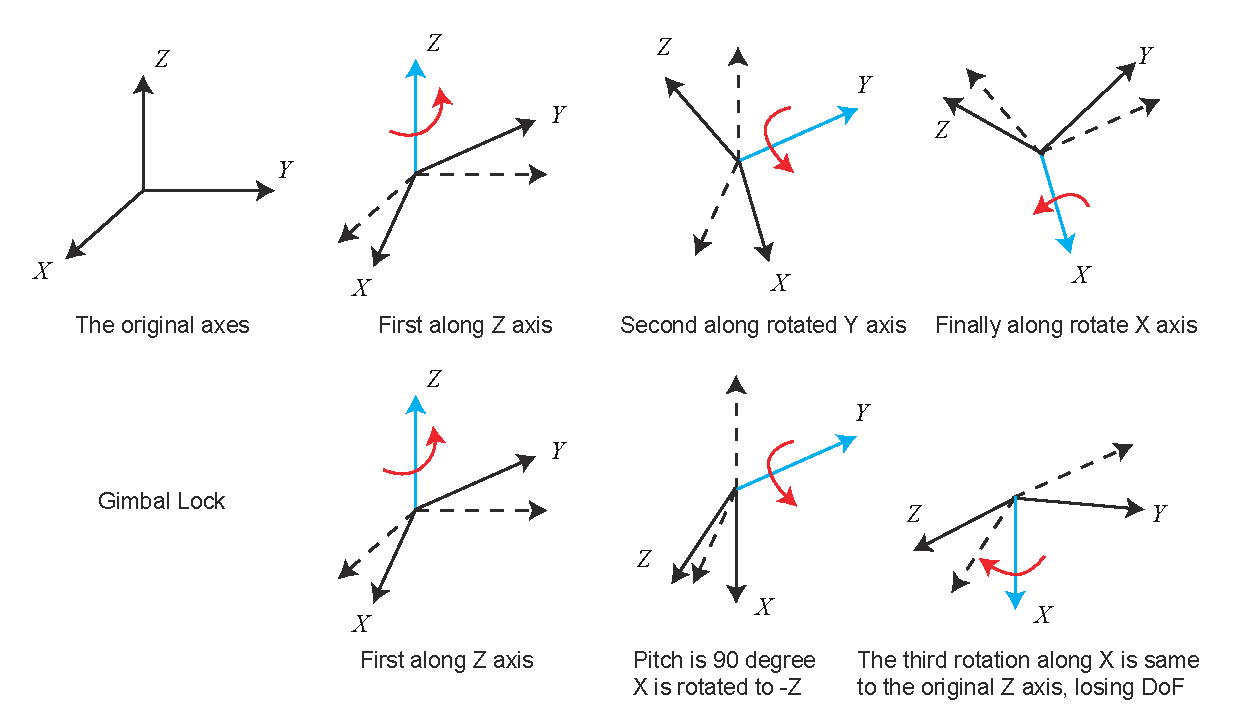
\includegraphics[width=1.0\textwidth]{rigidMotion/eulerAngles.pdf}
    \caption{Euler angles. The top is defined for the ZYX order (rpy order). The bottoms shows when pitch=$90^\circ$, the third rotation is using the same axis as the first one, causing the system to lose a degree of freedom. If you don't understand the universal lock, please take a look at the related videos and it will be more convenient to understand. }
    \label{fig:eulerAngles}
\end{figure}

In this way, we can use a three-dimensional vector such as $[r,p,y]^T$ to describe any rotation. This vector is very intuitive. We can imagine the rotation process from this vector. The other Euler angles are also decomposed into three axes to obtain a three-dimensional vector, but the axes and order may be different. The $rpy$ angle introduced here is a widely used one, and only a few Euler angles have such a famous name as $rpy$. Different Euler angles are referred to in the order of the axes of rotation. For example, the rotation order of the rpy angle is $ZYX$. Similarly, there are Euler angles like $XYZ, ZYZ$ - but they don't have a specific name. It is worth mentioning that most areas have their own coordinate directions and habits when using Euler angles, not necessarily the same as we said here.

A major drawback of Euler Angle is that it encounters the famous \textit{Gimbal lock} \footnote{See \url{https://en.wikipedia.org/wiki/Gimbal_lock}.}): in the $rpy$'s case, when the pitch angle is $\pm 90 ^\circ $, the first rotation and the third rotation will use the same axis, causing the system to lose a degree of freedom (from 3 rotations to 2 rotations). This is called the singularity problem and also exists in other forms of Euler angles. In theory, it can be proved that as long as you want to use three real numbers to express the three-dimensional rotation, you will inevitably encounter the singularity problem. \footnote{The rotation vector also has a singularity, which occurs when the angle $\theta$ exceeds $2\pi$. Obviously, rotating $2\pi$ is the same with no rotation.} Due to this fact, Euler angles are not suitable for interpolation or iterations, and are often only used in human-computer interaction. We rarely use Euler angles to express poses directly in the SLAM program, nor do we use Euler angles to describe rotation in filtering or optimization (because it has singularity). However, if you want to verify that your algorithm is correct or not, converting to Euler angles can help you quickly determine if the results are correct or not. In some cases where the main body is mainly 2D motion (such as sweepers, self-driving vehicles), we can also decompose the rotation into three Euler angles and then take one of them (such as the yaw angle) as the orientation output.

\section{Quaternions}
The rotation matrix describes 3 degrees of freedom with 9 quantities, of course, with redundancy; the Euler angles and the rotation vectors are compact but suffer from the singularity. In fact, we \textit{cannot} find a three-dimensional vector description without singularity \cite{Stuelpnagel1964}. This is somewhat similar to using two coordinates to represent the Earth's surface (such as longitude and latitude), which also has the singularity (longitude is meaningless when the latitude is $ \pm  90 ^ \circ $ ).

Recall the complex number that we have studied before. We use the complex set $ \mathbb {C} $ to represent the vector on the 2D complex plane, and the complex multiplication with a unit complex number can represent the rotation on the 2D plane: for example, multiplying the complex $i$ is equivalent to rotating a complex vector counterclockwise by $ 90 ^ \circ $. Similarly, when expressing a three-dimensional space rotation, there is also an algebra similar to a complex number: the \textit{quaternions}. Quaternions are extended complex numbers found by Hamilton. It is both compact and not singular. If we must find some shortcomings, the quaternion is not intuitive enough, and its operation is a bit more complicated.

Comparing quaternions to complex numbers can help you understand quaternions faster. For example, when we want to rotate the vector of a complex plane by $\theta$, we can multiply this complex vector by $\mathrm{e}^{i \theta}$, which is represented by polar coordinates. It can also be written in the usual form like the famous Euler equation:
\begin{equation}
\mathrm{e}^{i\theta} = \cos \theta + i \sin \theta.
\end{equation}
This is a unit-length complex number. Therefore, in two dimensions, the rotation can be described by a unit complex number. Similarly, we will see that 3D rotation can be described by a unit quaternion.

A quaternion $ \mathbf{q} $ has a real part and three imaginary parts. We write the real part in the front (and there are also some books where the real part is in the last), like this:
\begin{equation}
\mathbf{q} = q_0 + q_1 i + q_2 j + q_3 k,
\end{equation}
where $ i,j,k $ are three imaginary parts of the quaternion. These three imaginary parts satisfy the following relationship:
\begin{equation}
\label{eq:quaternionVirtual}
\left\{ \begin{array}{l}
{i^2} = {j^2} = {k^2} =  - 1\\
ij = k, ji = - k \\
jk = i,kj =  - i\\
ki = j, ik = - j
\end{array} \right. .
\end{equation}
If we look at $ i, j, k $ as three axes, they look the same as complex numbers when multiplying with themselves. And look the same as the outer product when multiplying with the others. 

We can also use a scalar and a vector to express quaternions:
\[
\mathbf{q} = \left[ s, \mathbf{v} \right]^T, \quad s=q_0 \in \mathbb{R},\quad \mathbf{v} = [q_1, q_2, q_3]^T \in \mathbb{R}^3,
\]
Here, $ s $ is the real part of the quaternion, and $ \mathbf {v} $ is its imaginary part. If the imaginary part of a quaternion is $ \mathbf {0} $, it is called \textit{real quaternion}. Conversely, if its real part is $ 0 $, it is called \textit{imaginary quaternion}.

We can use a unit quaternion to represent any rotation in 3D space, but this expression is subtly different from the complex numbers. In the complex, multiplying by $ i $ means rotating $ 90 ^ \circ $. Does this mean that in the quaternion, multiplied by $ i $ is rotating around the $ i $ axis by $ 90 ^ \circ $ ? So, does $ ij = k $ means, first rotating around the $ i $ by $ 90 ^ \circ $, then around $j$ by $ 90 ^ \circ $, is equivalent to rotating around $ k$ by $ 90 ^ \circ $ ? Readers can use a cell phone to simulate that, then you will find that this is not the right case. The correct situation should be that multiplying $ i $ corresponds to rotating $ 180 ^ \circ $, in order to guarantee the nature of $ ij=k $. And $ i^ 2 =- 1 $ means that after rotating $ 360 ^ \circ $ around the $ i $ axis, we get an opposite thing. This object has to be rotated by 720 $^\circ$ to be equal to its original appearance.

This seems a bit mysterious. The complete explanation needs too many extra things. Let's calm down and come back to the quaternions. At least, we know that a unit quaternion can express the rotation of a three-dimensional space. So what are the properties of the quaternions? And how can they operate with each other?

\subsection{Quaternion Operations}
Quaternions are very similar to complex numbers, and a series of quaternion operations can be performed. We can easily plus, minus, multiplies to quaternions just like doing with two complex numbers. Assume there are two quaternions $ \mathbf{q}_a, \mathbf{q}_b $, whose vectors are represented as $ [s_a, \mathbf {v}_a]^ \mathrm {T}, [s_b, \mathbf{v}_b]^ \mathrm {T} $, or the original quaternion is expressed as:
\[
\mathbf{q} _a = s_a + x_ai + y_aj + z_ak, \quad  \mathbf {q} _b = s_b + x_bi + y_bj + z_bk.
\]
Then, their operations can be expressed as follows.

\begin{enumerate}
    \item { \textbf{Addition and subtraction}.} The addition and subtraction of the quaternion $ \mathbf {q}_a, \mathbf {q}_b $ is:
    \begin{equation} 	
    \mathbf{q}_a \pm \mathbf{q}_b = \left[ s_a \pm s_b, \mathbf{v}_a \pm \mathbf{v}_b \right]^T.
    \end{equation}
    \item { \textbf {Multiplication}}. Quaternion multiplication is the multiplication of each item of $ \mathbf {q}_a $ with each item of $ \mathbf {q}_b $. The imaginary part is done according to  formula~\eqref {eq:quaternionVirtual}:
    \begin{equation}
    \begin{aligned}
    \mathbf{q}_a \mathbf{q}_b &= {s_a}{s_b} - {x_a}{x_b} - {y_a}{y_b} - {z_a}{z_b}\\
    &+ \left( {{s_a}{x_b} + {x_a}{s_b} + {y_a}{z_b} - {z_a}{y_b}} \right)i\\
    &+ \left( {{s_a}{y_b} - {x_a}{z_b} + {y_a}{s_b} + {z_a}{x_b}} \right)j\\
    &+ \left( {{s_a}{z_b} + {x_a}{y_b} - {y_a}{x_b} + {z_a}{s_b}} \right)k.
    \end{aligned}
    \end{equation}
    
    The scalar form is a little complicated, but the vector form is more concise:
    \begin{equation}
    \mathbf{q}_a \mathbf{q}_b = \left[ s_a s_b - \mathbf{v}_a^T \mathbf{v}_b, s_a\mathbf{v}_b + s_b\mathbf{v}_a + \mathbf{v}_a \times \mathbf{v}_b \right]^T.
    \end{equation}
    
    Under this multiplication definition, the product of two real quaternions is still real, which is also consistent with the real number multiplication. However, note that due to the existence of the last outer product, quaternion multiplication is usually not commutative unless $ \mathbf {v}_a $ and $ \mathbf {v}_b $ at $ \mathbb {R}^ 3 $ are parallel, which means the outer product term is zero.
    
    \item { \textbf {Length}. } The length of a quaternion is defined as:
    \begin{equation}
    \| \mathbf{q}_a \| = \sqrt{ s_a^2 + x_a^2 + y_a^2 + z_a^2 }.
    \end{equation}
    It can be verified that the length of the product is the product of the lengths. This makes the unit quaternion keep unit-length when multiplied by another unit quaternion:
    \begin{equation}
    \| \mathbf{q}_a \mathbf{q}_b \| = \|\mathbf{q}_a \| \| \mathbf{q}_b \|.
    \end{equation}
    
    \item { \textbf {Conjugate}}. The conjugate of a quaternion is to take the imaginary part as the opposite:
    \begin{equation}
    \mathbf{q}_a ^ * = s_a - x_ai - y_aj - z_ak = [s_a, - \mathbf{v}_a] ^T.
    \end{equation}
    We get a real quaternion if the quaternion is multiplied by its conjugate. The real part is the square of its length:
    \begin{equation}
    \mathbf{q}^* \mathbf{q} = \mathbf{q} \mathbf{q}^* = [s^2+\mathbf{v}^T \mathbf{v}, \mathbf{0} ]^T.
    \end{equation}
    
    \item { \textbf{Inverse}}. The inverse of a quaternion is:
    \begin{equation}
    \label{eq:quaternionInverse}
    \mathbf{q} ^ { - 1 } = \mathbf{q} ^ * / \| \mathbf{q} \| ^ 2.
    \end{equation}
    According to this definition, the product of the quaternion and its inverse is the real quaternion $ \mathbf {1} $ :
    \begin{equation}
    \mathbf{q} \mathbf{q}^{-1} = \mathbf{q}^{-1} \mathbf{q} = \mathbf{1}.
    \end{equation}
    
    If $ \mathbf{q} $ is a unit quaternion, its inverse and conjugate are the same. So the inverse of the product has properties similar to matrices:
    \begin{equation}
    \left( \mathbf{q}_a \mathbf{q}_b \right)^{-1} = \mathbf{q}_b^{-1} \mathbf{q}_a^{-1}.
    \end{equation}
    
    \item { \textbf {Scalar Multiplication}.} Similar to vectors, quaternions can be multiplied by numbers:
    \begin{equation}
    k \mathbf{q} = \left[ ks, k\mathbf{v} \right]^T.
    \end{equation}
\end{enumerate}

\subsection{Use Quaternion to Represent a Rotation}

We can use a quaternion to express the rotation of a point. Suppose a spatial 3D point $ \mathbf{p} = [x,y,z]^T \in  \mathbb {R}^3$, and a rotation is specified by a unit quaternion $ \mathbf{q}$. The 3D point $\mathbf{p}$ is rotated to become $\mathbf{p}'$. If we use matrix, then there is $ \mathbf{p}'= \mathbf{R} \mathbf{p} $. And if we use quaternion to describe rotation, how do we operate a 3D vector with a quaternion?

First, we extend the 3D point to an imaginary quaternion:
\[
\mathbf{p} = [0, x, y, z]^T = [0, \mathbf{v}]^T. 
\]
We just put the three coordinates into the imaginary part and leave the real part to be zero. Then, the rotated point $ \mathbf {p}' $ can be expressed as such a product:

\begin{equation}\label{eq:rotate-with-quaternion}
\mathbf{p}' = \mathbf{q} \mathbf{p} \mathbf{q}^{-1}.
\end{equation}

The multiplication here is the quaternion multiplication, and the result is also a quaternion. Finally, we take the imaginary part of $ \mathbf{p}' $ and get the coordinates of the point after the rotation. It can be easily verified (we leave as an exercise here) that the real part of the calculation is 0, so it is a pure imaginary quaternion.

\subsection{Conversion of Quaternions to Other Rotation Representations}

An arbitrary unit quaternion describes a rotation, which can also be described by a rotation matrix or a rotation vector. Now let's examine the conversion relationship between quaternions and rotation vectors/matrices. Before that, we have to say that quaternion multiplication can also be written as a matrix multiplication. Let $\mathbf{q}=[s,\mathbf{v}]^T$, then define the following symbols $^{+}$ and $^{\oplus}$ as~\cite{Barfoot2011}:
\begin{equation}
	\mathbf{q}^{+}=\left[\begin{array}{cc}
		s&-\mathbf{v}^T \\
		\mathbf{v}&s\mathbf{I}+\mathbf{v}^{\wedge}
	\end{array}\right],\quad
	\mathbf{q}^{\oplus}=
	\left[\begin{array}{cc}
		s & -\mathbf{v}^T \\
		\mathbf{v} & s\mathbf{I}-\mathbf{v}^{\wedge}
	\end{array}\right],
\end{equation}
These two symbols map the quaternion to a 4$\times$4 matrix. Then the quaternion multiplication can be written in the form of a matrix:
\begin{equation}
	\mathbf{q}_1^ + {\mathbf{q}_2} = \left[ {\begin{array}{*{20}{c}}
			s_1&-\mathbf{v}_1^T\\
			\mathbf{v}_1 & s_1 \mathbf{I} + \mathbf{v}_1^\wedge
	\end{array}} \right]\left[ {\begin{array}{*{20}{c}}
			{{s _2}} \\
			{{\mathbf{v} _2}}
	\end{array}} \right] = \left[ {\begin{array}{*{20}{c}}
			{ - \mathbf{v} _1^T{\mathbf{v} _2} + {s _1}{s _2}} \\
			{{s _1}{\mathbf{v} _2} + {s _2}{\mathbf{v} _1} + \mathbf{v} _1^ \wedge {\mathbf{v} _2}}
	\end{array}} \right] = \mathbf{q}_1 \mathbf{q}_2
\end{equation}
Note that the left side is matrix multiplication and the right side is quaternion multiplication. Similar for $^\oplus$, we get:
\begin{equation}
	\mathbf{q}_1 \mathbf{q}_2 = \mathbf{q}_1^{+} \mathbf{q}_2 = \mathbf{q}_2^{\oplus} \mathbf{q}_1.
\end{equation}

Then, consider the problem of using a quaternion to rotate a spatial point. According to the previous section, we have:
\begin{equation}
	\begin{split}
		\mathbf{p}' &= \mathbf{q} \mathbf{p} \mathbf{q}^{-1} = \mathbf{q}^+ \mathbf{p}^+ \mathbf{q}^{ -1} \\
		&= \mathbf{q}^+ \mathbf{q}^{{-1}^{\oplus}} \mathbf{p}.
	\end{split}
\end{equation}
Substituting the matrix corresponding to two symbols, we get:
\begin{equation}\label{eq:quaternion-to-rotation-matrix-derive}
	{\mathbf{q}^ + }{\left( {{\mathbf{q}^{ - 1}}} \right)^ \oplus } = \left[ \begin{array}{*{20}{c }}
		s&-\mathbf{v}^T\\
		\mathbf{v}&s\mathbf{I}+\mathbf{v}^\wedge
	\end{array} \right]\left[\begin{array}{*{20}{c}}
		s&{\mathbf{v} ^T}\\
		{ - \mathbf{v} }&{s\mathbf{I} + \mathbf{v} ^ \wedge }
	\end{array} \right] = \left[ \begin{array}{*{20}{c}}
		1&\mathbf{0} \\
		\mathbf{0}^T&\mathbf{v}\mathbf{v}^T + {s^2} \mathbf{I} + 2s\mathbf{v} ^ \wedge + {(\mathbf{v} ^ \wedge)}^2
	\end{array} \right].
\end{equation}
Since $\mathbf{p}'$ and $\mathbf{p}$ are both imaginary quaternions, so in fact that the bottom right corner of the matrix gives the transformation formula \textit{from quaternion to rotation matrix} :
\begin{equation}
	\mathbf{R} = \mathbf{v} \mathbf{v}^T + {s^2} \mathbf{I} + 2s\mathbf{v} ^ \wedge + {(\mathbf{v } ^ \wedge)}^2.
\end{equation}
In order to obtain the conversion formula of the quaternion to the rotation vector, we take the trace on both sides of the above formula:
\begin{equation}
	\begin{aligned}
		\mathrm{tr}(\mathbf{R}) &= \mathrm{tr}(\mathbf{v}\mathbf{v}^T) + 3s^2 + 2s \cdot 0 + \mathrm{tr }((\mathbf{v}^\wedge)^2) \\
		&= v_1^2+v_2^2+v_3^2 + 3s^2 - 2(v_1^2+v_2^2+v_3^2) \\
		&= (1-s^2) + 3s^2 -2(1-s^2)\\
		&= 4s^2 -1.
	\end{aligned}
\end{equation}
Also obtained by the formula~\eqref{eq:R2theta}:
\begin{equation}
	\begin{aligned}
		\theta &= \arccos(\frac{\mathrm{tr}(\mathbf{R})-1}{2}) \\
		&=\arccos(2s^2-1),
	\end{aligned}
\end{equation}
which means:
\begin{equation}
	\cos \theta =2s^2-1=2 \cos^2 \frac{\theta}{2} -1,
\end{equation}
and so we have:
\begin{equation}
	\theta = 2 \arccos s.
\end{equation}
For the rotation axis, if we replace $\mathbf{p}$ with the imaginary part of $\mathbf{q}$ in the formula~\eqref{eq:quaternion-to-rotation-matrix-derive}, it is easy to know the imaginary part of  $\mathbf{q}$ is not moving when it is rotated, that is, it constitutes exactly the rotation axis. So we get the rotation axis just by normalizing $\mathbf{q}$'s imaginary part. In summary, the conversion formula from quaternion to rotation vector can be written as follows:
\begin{equation}
	\label{eq:rotationVector2Quaternion}
	\begin{cases}
		\theta = 2\arccos {q_0}\\
		{\left[ {{n_x},{n_y},{n_z}} \right]^T} = {{{\left[ {{q_1},{q_2},{q_3}} \right] }^T}}/{\sin \frac{\theta }{2}}
	\end{cases} .
\end{equation}

And for converting from other representations to quaternions, we only need to reversely follow the above steps. In actual programming, the library usually prepares for the conversion between various forms for us. Whether it's a quaternion, a rotation matrix, or an angle-axis, it can always be used to describe the same rotation. We should choose the most convenient form in practice without having to stick to a particular form. In the subsequent practices and exercises, we will demonstrate the transition between various expressions to deepen the reader's impression.

\section{Affine and Projective Transformation}
In addition to the Euclidean transformation, there are several other transformations in the 3D space, where the Euclidean is the simplest. Some of them are related to camera geometry. We will introduce them in the following chapters, so here we only list their basic properties. The Euclidean transformation keeps the vector's length and angle, which is equivalent to moving or rotating a rigid body without changing its appearance. The other transformations will change their shape, and they all have similar matrix representations.

\begin{enumerate}
	\item {\textbf{Similarity transformation}}.
	
	The similarity transformation has one more degree of freedom than the Euclidean transformation, which allows the object to be uniformly scaled, and its matrix is ​​expressed as:
	\begin{equation}
	\mathbf{T}_S = \left[ {\begin{array}{*{20}{c}}
		{s \mathbf{R}}& \mathbf{t}\\
		{{ \mathbf{0}^T}}&1
		\end{array}} \right].
	\end{equation}
	
	Note that the rotation part has an extra scaling factor $s$, which means that we can evenly scale the three coordinates of $x,\ y,\ and\ z$ of a vector after it is rotated. Due to the scaling, a similarity transformation no longer keeps the volume of ​​the transformed boy unchanged. You can imagine a cube with a side length of 1 transforming into a side with a length of 10 (but still being a cube). The set of three-dimensional similarity transform is also called \textit{similarity transform group}, which is denoted as $\mathrm{Sim}(3)$.
	
	\item {\textbf{Affine transformation}}.
	
	The matrix form of the affine transformation is as follows:
	\begin{equation}
	\mathbf{T}_A = \left[ {\begin{array}{*{20}{c}}
		\mathbf{A} & \mathbf{t}\\
		{{\mathbf{0}^T}} & 1
		\end{array}} \right].
	\end{equation}
	

	Unlike the Euclidean transformation, the affine transformation requires only $\mathbf{A}$ to be an invertible matrix, not necessarily an orthogonal matrix. An affine transformation is also called an orthogonal projection. After the affine transformation, the cube is no longer square, but the faces are still parallelograms.	
	
	\item{ \textbf{Perspective transformation}. }
	
	Perspective transformation is the most general transformation. Its matrix form is:
	
	\begin{equation}
	{\mathbf{T}_P} = \left[ {\begin{array}{*{20}{c}}
		\mathbf{A} & \mathbf{t}\\
		{{\mathbf{a}^T}} & v
		\end{array}} \right].
	\end{equation}
	
	Its upper left corner is the invertible matrix $\mathbf{A}$. The upper right corner is the translation $\mathbf{t}$, and the lower-left corner is the scale $\mathbf{a}^T$. Since the homogeneous coordinates are used, when $v \neq 0$, we can divide the entire matrix by $v$ to get a matrix with a bottom right corner of 1; otherwise, we get a matrix with a lower right corner of $0$. Therefore, the 2D perspective transformation has a total of 8 degrees of freedom, and 3D has a total of 15 degrees of freedom. Perspective transformation is the most general transformation that has been said so far. The transformation from the real world to a camera photo can be seen as a perspective transformation. The reader can imagine what a square tile would look like in a photo: first, it is no longer square. Second, since the close part is larger than the far-away part, it is not even a parallelogram but an irregular quadrilateral. 
\end{enumerate}

\autoref{table:common-transform} summarizes the properties of several transformations currently covered. Note that in the ``invariance'', there is an inclusion relationship from top to bottom. For example, in addition to maintaining volume, the Euclidean transformation also keeps the parallelism, intersection, and others.

\begin{table}[!htp]
	\centering
	\caption{comparison of common transformation properties}
	\label{table:common-transform}
	\small
	\begin{tabular}{c|c|c|c}
		\toprule
		Transform Name & Matrix Form & Degrees of Freedom & Invariance \\ \midrule
		Euclidean \rule{0pt}{20 pt} & $\left[ {\begin{array}{*{20}{c}}
			\mathbf{R} & \mathbf{t}\\
			{{\mathbf{0}^T}}&1
			\end{array}} \right]$ & 6 & Length, angle, volume \\
		Similarity \rule{0pt}{20 pt}& $ \left[ {\begin{array}{*{20}{c}}
			{s \mathbf{R}}& \mathbf{t}\\
			{{ \mathbf{0}^T}}&1
			\end{array}} \right]$ & 7 & volume ratio \\
		Affine \rule{0pt}{20 pt}& $ \left[ {\begin{array}{*{20}{c}}
			\mathbf{A} & \mathbf{t}\\
			{{\mathbf{0}^T}} & 1
			\end{array}} \right]$ & 12 & Parallelism, volume ratio \\
		Perspective \rule{0pt}{20 pt} & $ \left[ {\begin{array}{*{20}{c}}
			\mathbf{A} & \mathbf{t}\\
			{{\mathbf{a}^T}} & v
			\end{array}} \right]$ & 15 & Plane intersection and tangency \rule{0pt}{20 pt}\\
		\bottomrule
	\end{tabular}
\end{table}

We will introduce later that the transformation from the real world to the camera photo is a perspective transformation. If the focal length of the camera is infinity, then this transformation is affine. However, before we go into the camera model's details, let's do some experiments to have a rough impression of these transformations.

\section{Practice: \textit{Eigen} Geometry Module}
\subsection{Data Structure of the \textit{Eigen} Geometry Module}
Now, let's actually practice the various rotation expressions mentioned earlier. We will use quaternions, Euler angles, and rotation matrices in \textit{Eigen} to demonstrate how they are transformed. We will also provide a visualization program to help the reader understand the relationship between these transformations.

\begin{lstlisting}[language=c++,caption=slambook2/ch3/useGeometry/useGeometry.cpp]
#include <iostream>
#include <cmath>
using namespace std;

#include <Eigen/Core>
#include <Eigen/Geometry>

using namespace Eigen;
// This program demonstrates how to use the Eigen geometry module

int main(int argc, char **argv) {
	// The Eigen/Geometry module provides a variety of rotation and translation representations
	// 3D rotation matrix directly using Matrix3d or Matrix3f
	Matrix3d rotation_matrix = Matrix3d::Identity();
	// The rotation vector uses AngleAxis, the underlying layer is not directly Matrix, but the operation can be treated as a matrix (because the operator is overloaded)
	AngleAxisd rotation_vector(M_PI / 4, Vector3d(0, 0, 1)); // Rotate 45 degrees along the Z axis
	cout.precision(3);
	cout << "rotation matrix = \n " << rotation_vector.matrix() << endl; // convert to matrix with matrix()
	// can also be assigned directly
	rotation_matrix = rotation_vector.toRotationMatrix();
	// coordinate transformation with AngleAxis
	Vector3d v(1, 0, 0);
	Vector3d v_rotated = rotation_vector * v;
	cout << "(1,0,0) after rotation (by angle axis) = " << v_rotated.transpose() << endl;
	// Or use a rotation matrix
	v_rotated = rotation_matrix * v;
	cout << "(1,0,0) after rotation (by matrix) = " << v_rotated.transpose() << endl;
	
	// Euler angle: You can convert the rotation matrix directly into Euler angles
	Vector3d euler_angles = rotation_matrix.eulerAngles(2, 1, 0); // ZYX order, ie roll pitch yaw order
	cout << "yaw pitch roll = " << euler_angles.transpose() << endl;
	
	// Euclidean transformation matrix using Eigen::Isometry
	Isometry3d T = Isometry3d::Identity(); // Although called 3d, it is essentially a 4*4 matrix
	T.rotate(rotation_vector); // Rotate according to rotation_vector
	T.pretranslate(Vector3d(1, 3, 4)); // Set the translation vector to (1,3,4)
	cout << "Transform matrix = \n" << T.matrix() << endl;
	
	// Use the transformation matrix for coordinate transformation
	Vector3d v_transformed = T * v; // Equivalent to R*v+t
	cout << "v tranformed = " << v_transformed.transpose() << endl;
	
	// For affine and projective transformations, use Eigen::Affine3d and Eigen::Projective3d.
	
	// Quaternion
	// You can assign AngleAxis directly to quaternions, and vice versa
	Quaterniond q = Quaterniond(rotation_vector);
	cout << "quaternion from rotation vector = " << q.coeffs().transpose() << endl; 
	// Note that the order of coeffs is (x, y, z, w), w is the real part, the first three are the imaginary part
	// can also assign a rotation matrix to it
	q = Quaterniond(rotation_matrix);
	cout << "quaternion from rotation matrix = " << q.coeffs().transpose() << endl;
	// Rotate a vector with a quaternion and use overloaded multiplication
	V_rotated = q * v; // Note that the math is qvq^{-1}
	cout << "(1,0,0) after rotation = " << v_rotated.transpose() << endl;
	// expressed by regular vector multiplication, it should be calculated as follows
	cout << "should be equal to " << (q * Quaterniond(0, 1, 0, 0) * q.inverse()).coeffs().transpose() << endl;
	
	return 0;
}
\end{lstlisting}

The various forms of expression in \textit{Eigen} are summarized below. Note that each type has both single and double data types and, as before, cannot be automatically converted by the compiler. Taking the double-precision as an example, you can simply change the last ``d'' to ``f'' to use a single-precision data structure.
\begin{itemize}
	\item Rotation matrix ( $ 3  \times  3 $ ): Eigen::Matrix3d.
	\item Rotation vector ( $ 3  \times  1 $ ): Eigen::AngleAxisd.
	\item Euler angle ( $ 3  \times  1 $ ): Eigen::Vector3d.
	\item Quaternion ( $ 4  \times  1 $ ): Eigen::Quaterniond.
	\item Euclidean transformation matrix ( $ 4  \times  4 $ ): Eigen::Isometry3d.
	\item Affine transform ( $ 4  \times  4 $ ): Eigen::Affine3d.
	\item Perspective transformation ( $ 4  \times  4 $ ): Eigen::Projective3d.
\end{itemize}

This program can be compiled by referring to the corresponding ``CMakeLists.txt'' in the code. This program demonstrates how to use the rotation matrix, rotation vectors (AngleAxis), Euler angles, and quaternions in \textit{Eigen}. We use these rotations to rotate a vector $ \mathbf {v} $ and find that the result is the same. At the same time, it also demonstrates how to convert these expressions in the program. Readers who want to learn more about \textit{Eigen}'s geometry modules can refer to \url {http://eigen.tuxfamily.org/dox/group__TutorialGeometry.html}.

Note that the code has some subtle differences from the mathematical representation. For example, by operator overloading in C++, quaternions and three-dimensional vectors can directly be multiplied, but mathematically, the vector needs to be converted into an imaginary quaternion, as we talked about in the last section, and then quaternion multiplication is used for calculation. The same applies to the transformation matrix multiplying with a three-dimensional vector. In general, the usage in the program is more flexible than the mathematical formula.

\subsection{Coordinate Transformation Example}

Let's take a small example to demonstrate the coordinate transformation.

\noindent  \textit{Example 1}. \quad  The robot No.1 and the robot No.2 are located in the world coordinate system. We use the world coordinate system as $W$, robot coordinate system as $R_1 $ and $R_2$. The pose of the robot 1 is $ \mathbf {q}_ 1 = [ 0.35, 0.2, 0.3, 0.1 ]^T, \mathbf{t}_ 1 = [ 0.3, 0.1, 0.1 ]^T $. The pose of the robot 2 is $ \mathbf{q}_2 = [ - 0.5, 0.4, - 0.1, 0.2 ]^T, \mathbf{t}_ 2 = [- 0.1, 0.5, 0.3 ]^T $. Here $ \mathbf {q} $ and $ \mathbf{t} $ express $ \mathbf{T}_{R_k, W}, k= 1, 2 $, which is the world to the robot transform matrix. Now, assume that robot 1 sees a point in its own coordinate system with coordinates of $ \mathbf{p}_{R_1} = [ 0.5, 0, 0.2 ]^T $. We want to find the coordinates of the vector in the robot 2's coordinate system.

This is a very simple but representative example. In real scenarios you often need to convert coordinates between different parts of the same robot or between different robots. Below we write a program to demonstrate this calculation.

\begin{lstlisting}[language=c++,caption=slambook2/ch3/examples/coordinateTransform.cpp]
#include<iostream>
#include<vector>
#include<algorithm>
#include<Eigen/Core>
#include<Eigen/Geometry>

using namespace std;
using namespace Eigen;

int main(int argc, char** argv) {
	Quaterniond q1(0.35, 0.2, 0.3, 0.1), q2(-0.5, 0.4, -0.1, 0.2);
	q1.normalize();
	q2.normalize();
	Vector3d t1(0.3, 0.1, 0.1), t2(-0.1, 0.5, 0.3);
	Vector3d p1(0.5, 0, 0.2);
	
	Isometry3d T1w(q1), T2w(q2);
	T1w.pretranslate (t1);
	T2w.pretranslate (t2);
	
	Vector3d p2 = T2w * T1w.inverse() * p1;
	cout << endl << p2.transpose() << endl;
	return 0;
}
\end{lstlisting}

The answer to the program is $ [- 0.0309731, 0.73499, 0.296108 ]^T$, and the calculation process is very simple, just by calculating $$ \mathbf{p}_{R_2} = \mathbf{T}_{ R_2, W} \mathbf{T}_{W, R_1} \mathbf{p}_{R_1}. $$ Note that the quaternion needs to be normalized before use.

\section{Visualization Demo}
\subsection{Plotting Trajectory}
If you are new to rotation and translation concepts, you may find that their form looks a little complicated. There are so many representation methods, and we need to convert to a preferred one if necessary. Fortunately, although the rotation and transformation matrix values may not be intuitive enough, we can easily draw them in a 3D window.

In this section, we demonstrate two visual examples. First, let's say that we recorded the trajectory of a robot somehow, and now we want to draw it in a figure. Suppose the trajectory file is stored in a text file called ``trajectory.txt'', and each line is stored in the following format: $$ \mathrm {time}, t_x, t_y, t_z, q_x, q_y, q_z, q_w, $$ where $ \mathrm {time} $ refers the recording time of this pose, $ \mathbf {t} $ is translation, $ \mathbf {q} $ is the quaternion, all recorded in the world coordinate system to the robot coordinate system. Below we read these tracks from the file and display them in a window. In principle, if we just talk about ``robot pose'', then we can use any one of $ \mathbf {T}_{WR} $ or $ \mathbf {T}_{RW} $ because they are just the inverse of each other. It means that knowing one of them makes it easy to get the other. If we want to store \textit {robot's trajectory}, then saving $ \mathbf {T}_{WR} $ or $ \mathbf {T}_{RW} $ doesn't make much difference.

When drawing the trajectory, we should draw the ``trajectory'' as a sequence of points, which is similar to the ``trajectory'' we imagined. Strictly speaking, these are actually the coordinates of the robot's origin in the world coordinate system. Consider the origin of the robot coordinate system, i.e., $ \mathbf {O}_{R}$, then the $ \mathbf{O}_{W}$ at this time is the coordinates of the origin in the world coordinate system:
\begin{equation}
\mathbf{O} _ {W} = \mathbf{T} _ {WR} \mathbf {O} _R = \mathbf {t} _ {WR}.
\end{equation}
This is exactly the translation part of $ \mathbf {T}_{WR} $. So, you can see the robot's position directly from $ \mathbf {T}_{WR} $. Therefore, in most of the public datasets, the trajectory file stores $ \mathbf {T}_{WR} $ instead of $ \mathbf {T}_{RW} $ .

Finally, we need a library that supports 3D drawing. Many libraries support 3D drawing, such as the famous Matlab, python matplotlib, OpenGL, etc. In Linux, a widely used library in SLAM is the OpenGL-based \textit{Pangolin} library \footnote{See \url {https://github.com/stevenlovegrove/Pangolin}.}, which provides simple OpenGL drawing operations in a window. In the second edition of the book, we used git's submodule feature to manage the third-party libraries that this book relies on. Readers can go directly to the ``3rdparty'' folder to install the required libraries, and git guarantees that you are using the same version with us.

\begin{lstlisting}[language=c++,caption=slambook2/ch3/examples/plotTrajectory.cpp]
#include <pangolin/pangolin.h>
#include <Eigen/Core>
#include <unistd.h>

using namespace std;
using namespace Eigen;

// path to trajectory file
string trajectory_file = "./examples/trajectory.txt";

void DrawTrajectory(vector<Isometry3d, Eigen::aligned_allocator<Isometry3d>>);

int main(int argc, char **argv) {
	vector<Isometry3d, Eigen::aligned_allocator<Isometry3d>> poses;
	ifstream fin(trajectory_file);
	if (!fin) {
		cout << "cannot find trajectory file at " << trajectory_file << endl;
		return 1;
	}
	
	while (!fin.eof()) {
		double time, tx, ty, tz, qx, qy, qz, qw;
		fin >> time >> tx >> ty >> tz >> qx >> qy >> qz >> qw;
		Isometry3d Twr(Quaterniond(qw, qx, qy, qz));
		Twr.pretranslate(Vector3d(tx, ty, tz));
		poses.push_back(Twr);
	}
	cout << "read total " << poses.size() << " pose entries" << endl;
	
	// draw trajectory in pangolin
	DrawTrajectory(poses);
	return 0;
}

void DrawTrajectory(vector<Isometry3d, Eigen::aligned_allocator<Isometry3d>> poses) {
	// create pangolin window and plot the trajectory
	pangolin::CreateWindowAndBind("Trajectory Viewer", 1024, 768);
	glEnable(GL_DEPTH_TEST);
	glEnable(GL_BLEND);
	glBlendFunc(GL_SRC_ALPHA, GL_ONE_MINUS_SRC_ALPHA);
	
	pangolin::OpenGlRenderState s_cam(
	pangolin::ProjectionMatrix(1024, 768, 500, 500, 512, 389, 0.1, 1000),
	pangolin::ModelViewLookAt(0, -0.1, -1.8, 0, 0, 0, 0.0, -1.0, 0.0)
	);
	
	pangolin::View &d_cam = pangolin::CreateDisplay()
	.SetBounds(0.0, 1.0, 0.0, 1.0, -1024.0f / 768.0f)
	.SetHandler(new pangolin::Handler3D(s_cam));
	
	while (pangolin::ShouldQuit() == false) {
		glClear(GL_COLOR_BUFFER_BIT | GL_DEPTH_BUFFER_BIT);
		d_cam.Activate(s_cam);
		glClearColor(1.0f, 1.0f, 1.0f, 1.0f);
		glLineWidth(2);
		for (size_t i = 0; i < poses.size(); i++) {
			// draw three axes of each pose
			Vector3d Ow = poses[i].translation();
			Vector3d Xw = poses[i] * (0.1 * Vector3d(1, 0, 0));
			Vector3d Yw = poses[i] * (0.1 * Vector3d(0, 1, 0));
			Vector3d Zw = poses[i] * (0.1 * Vector3d(0, 0, 1));
			glBegin(GL_LINES);
			glColor3f(1.0, 0.0, 0.0);
			glVertex3d (Ow [0], Ow [1], Ow [2]);
			glVertex3d (Xw [0], Xw [1], Xw [2]);
			glColor3f(0.0, 1.0, 0.0);
			glVertex3d (Ow [0], Ow [1], Ow [2]);
			glVertex3d (Is [0], Is [1], Is [2]);
			glColor3f(0.0, 0.0, 1.0);
			glVertex3d (Ow [0], Ow [1], Ow [2]);
			glVertex3d (Zw [0], Zw [1], Zw [2]);
			glEnd();
		}
		// draw a connection
		for (size_t i = 0; i < poses.size(); i++) {
			glColor3f(0.0, 0.0, 0.0);
			glBegin(GL_LINES);
			auto p1 = poses[i], p2 = poses[i + 1];
			glVertex3d(p1.translation()[0], p1.translation()[1], p1.translation()[2]);
			glVertex3d(p2.translation()[0], p2.translation()[1], p2.translation()[2]);
			glEnd();
		}
		pangolin::FinishFrame();
		usleep(5000);   // sleep 5 ms
	}
}
\end{lstlisting}

This program demonstrates how to draw a 3D pose in \textit{Pangolin}. We draw the three axes of each pose in red, green, and blue (actually, we calculate each axis's world coordinates) and then connect the poses with black lines. The result is shown in \autoref {fig:trajectory}.

\begin{figure}[!htp]
	\centering
	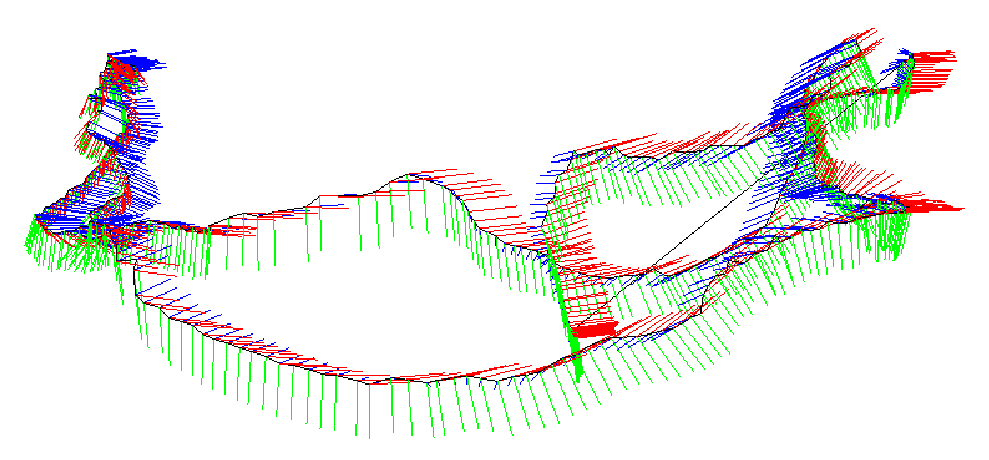
\includegraphics[width=0.8\textwidth]{rigidMotion/trajectory.pdf}
	\caption {Results of pose visualization}
	\label{fig:trajectory}
\end{figure}

\subsection{Displaying Camera Pose}
\begin{figure}[!htp]
	\centering
	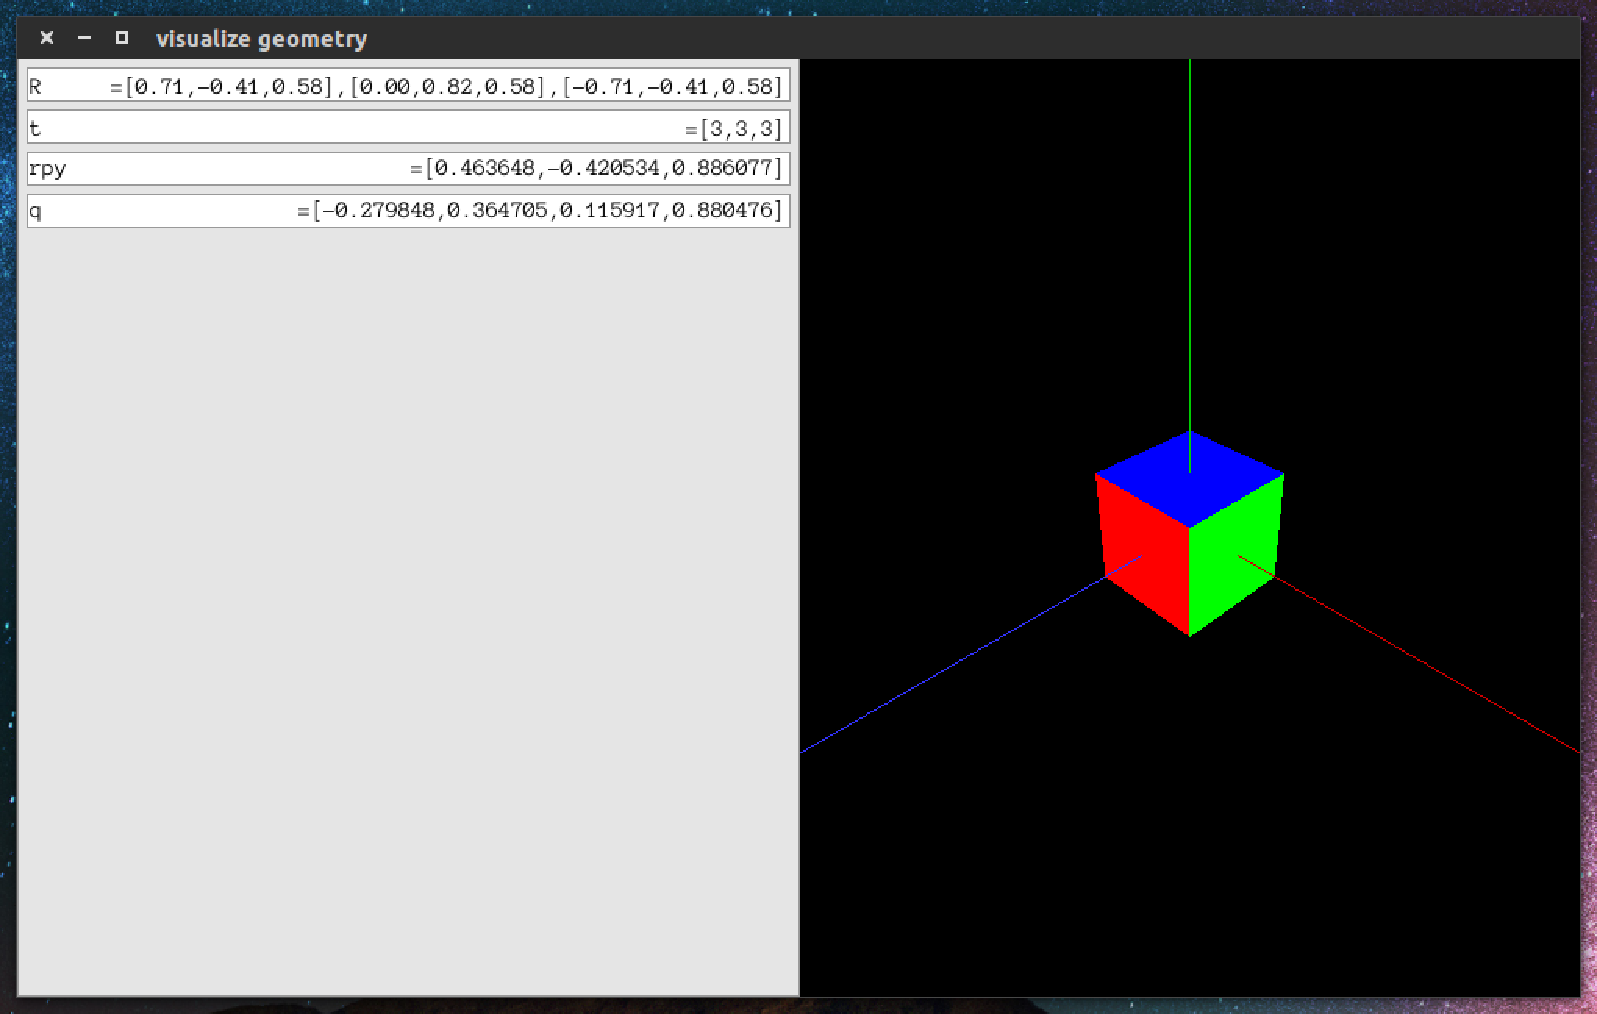
\includegraphics[width=0.8\textwidth]{rigidMotion/visualizeGeometry.pdf}
	\caption {Visualization program for rotation matrix, Euler angle, quaternion. }
	\label{fig:visualizeGeometry}
\end{figure}

In addition to displaying the trajectory, we can also display the camera's pose in the 3D window. In slambook2/ch3/visualizeGeometry, we visualize various expressions of camera poses (see \autoref{fig:visualizeGeometry}). When the reader uses the mouse to move the camera, the box on the left side will display the rotation matrix, translation, Euler angle, and quaternion of the camera pose in real-time. You can see how the data changes. According to our experience, it is hard to infer the exact rotation from quaternions or matrices. However, although the rotation matrix or transformation matrix is not intuitive, it is not difficult to visually display them. This program uses the \textit{Pangolin} library as a 3D display library. Please refer to ``Readme.txt'' to compile the program.

\section*{Exercises}
\begin{enumerate}
	\item Verify that the rotation matrix is an orthogonal matrix.
	\item Prove the Rodrigues formula.
	\item Verify that after the quaternion rotates a point, the result is a imaginary quaternion (the real part is zero), so it still corresponds to a three-dimensional space point, see~\eqref{eq:rotate-with-quaternion}.
	\item Draw a table that summarizes the conversion relationship of the rotation matrix, rotation angle, Euler angle and quaternion.
	\item Suppose there is a large \textit{Eigen} matrix, we want to know the value in the top left $3 \times 3$ blocks, and then assign it to $\mathbf{I}_{3 \times 3}$. Please implement it in C++.
	\item When does a general linear equation $\mathbf{A} \mathbf{x}=\mathbf{b}$ has a unique solution of $\mathbf{x}$? How to solve it numerically? Can you implement it in \textit{Eigen}?
\end{enumerate}

% !Mode:: "TeX:UTF-8"
\chapter{Lie Group and Lie Algebra}
\label{cpt:4}
\begin{mdframed}
    \textbf{Goal of Study}
    \begin{enumerate}
        \item Learn the concept of Lie group, Lie algebra, and their applications of $ \mathrm{SO}( 3 ), \mathrm{SE}( 3 ) $ and the corresponding Lie algebras.
        \item Learn the meaning and usage of the BCH (Baker-Campbell-Hausdorff) formula.
        \item Learn the perturbation model on Lie algebra.
        \item Use Sophus to perform operations on Lie algebras.
    \end{enumerate}
\end{mdframed}

In the last lecture, we introduced the description of rigid body motion in the three-dimensional world, including the rotation matrix, rotation vector, Euler angle, quaternion, and so on. We focused on the representation of rotation, but in SLAM, we have to estimate and optimize them in addition to the representation. Because the pose is unknown in SLAM, we need to solve the problem of which camera pose best matches the current observation. A typical way is to build it into an optimization problem, solving the optimal $ \mathbf{R}, \mathbf{t}$ and minimizing the error.

As mentioned before, the rotation matrix itself is a constrained (orthogonal, and the determinant is 1) matrix. When used as optimization variables, it introduces additional constraints on matrices that make optimization difficult. Through the transformation relationship between Lie group and Lie algebra, we can turn the pose estimation into an unconstrained optimization problem and simplify the solution. Considering that the reader may not have the basic knowledge of Lie Group and Lie algebra, we will start with the most basic knowledge.

\newpage
%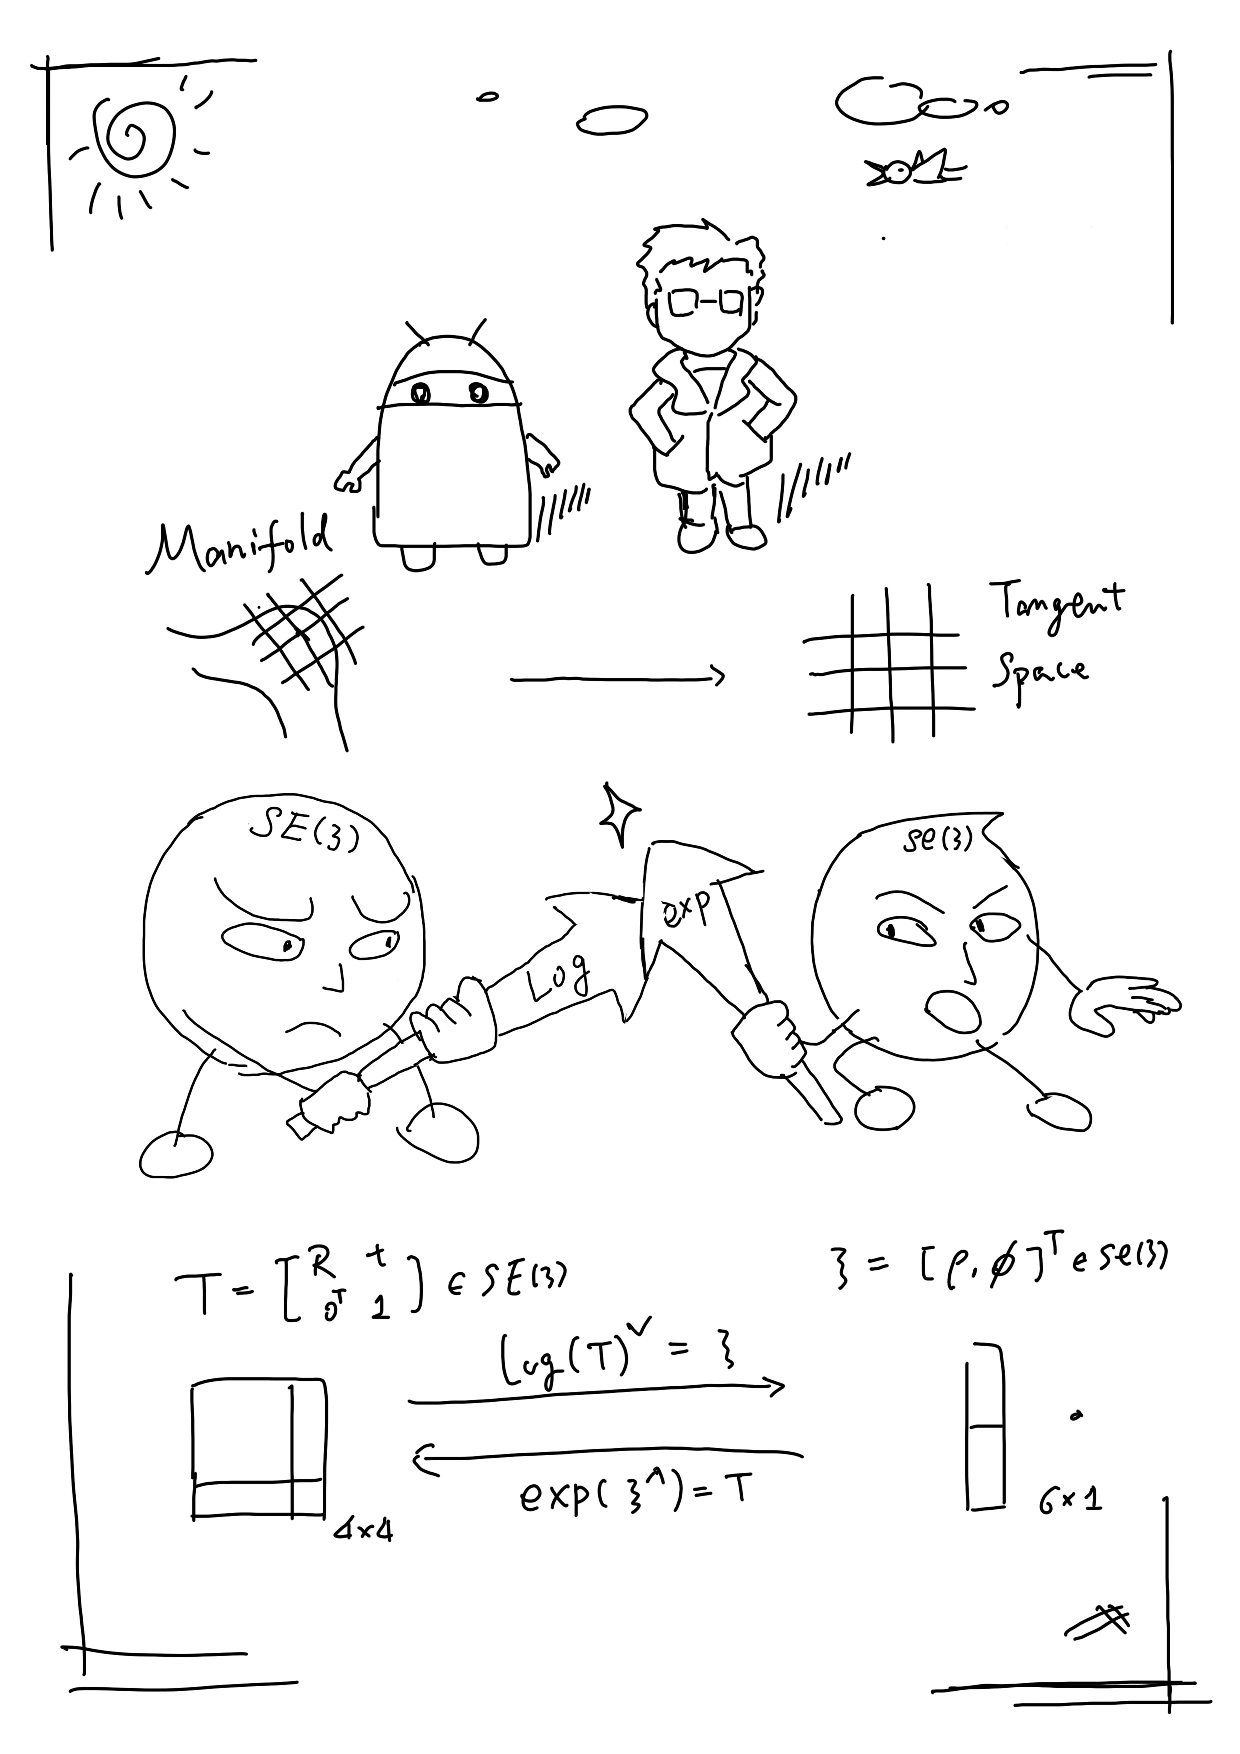
\includepdf{resources/other/ch4.pdf}
%\newpage

\section{Basics of Lie Group and Lie Algebra}
In the last lecture, we introduced the definition of the rotation matrix and the transformation matrix. At the time, we said that the three-dimensional rotation matrix constitutes the \textit{special orthogonal group} $\mathrm{SO}(3)$, and the transformation matrix constitutes the \textit{special Euclidean group} $\mathrm{SE}(3) $. They are written like this:
\begin{equation}
\mathrm{SO}(3) = \{ \mathbf{R} \in \mathbb{R}^{3 \times 3} | \mathbf{RR}^T = \mathbf{I}, \det(\mathbf{R})=1 \}.
\end{equation}
\begin{equation}
\mathrm{SE}(3) = \left\{ \mathbf{T} = \left[ {\begin{array}{*{20}{c}}
    \mathbf{R} & \mathbf{t} \\
    {{\mathbf{0}^T}} & 1
    \end{array}} \right]
\in \mathbb{R}^{4 \times 4} | \mathbf{R} \in \mathrm{SO}(3), \mathbf{t} \in \mathbb{R}^3\right\}.
\end{equation}

However, at that time, we did not explain the meaning of the group in detail. Readers should note that both the rotation matrix and the transformation matrix are not closed to addition. In other words, for any two rotation matrices $\mathbf{R}_1, \mathbf{R}_2$, according to the definition, their addition is no longer a rotation matrix:
\begin{equation}
\mathbf{R}_1 + \mathbf{R}_2 \notin \mathrm{SO}(3), \quad \mathbf{T}_1 + \mathbf{T}_2 \notin \mathrm{SE}(3).
\end{equation}
You can also say that the two matrices do not have a well-defined addition operator, or the matrix addition is not closed in these two sets. The multiplication is the only one closed operation in these sets:
\begin{equation}
\mathbf{R}_1 \mathbf{R}_2 \in \mathrm{SO}(3), \quad \mathbf{T}_1 \mathbf{T}_2 \in \mathrm{SE}(3).
\end{equation}
We know that matrix multiplication corresponds to the composition of two rotations or transformations. For a set that only has one ``well-defined'' operation, we call it a \textit{group}.

\subsection{Group}
For the following contents, we need to talk a little bit about abstract algebra. I think this is a necessary condition for discussing Lie Group and Lie Algebra, but in fact, except for the students of mathematics and physics, most of the students will not have this knowledge in undergraduate classes. So let's look at some basic concepts first.

A group is an algebraic structure of one set plus one operator. We denote the set as $A$ and the operation as $\cdot$, then the group can be denoted as $G=(A,\cdot)$. We say $G$ is a \textit{group} if the operation satisfies the following conditions:

\begin{enumerate}
    \item { \textbf{Closure}}: $ \  \forall a_1, a_2 \in A, \  a_1 \cdot a_2 \in A$.
    \item { \textbf{Combination}}: $ \  \forall a_1, a_2, a_3 \in A, \  (a_1 \cdot a_2) \cdot a_3 = a_1 \cdot ( a_2 \cdot a_3) $.
    \item { \textbf{Unit element}}: $ \  \exists a_0 \in A, \  \mathrm{s.t.} \ \forall a \in A, \  a_0 \cdot a = a \cdot a_0 = a $.
    \item { \textbf{Inverse element}}: $ \  \forall a \in A, \  \exists a^{-1} \in A, \  st \  a \cdot a^{-1} = a_0 $.
\end{enumerate}

It is easy to verify that the rotation matrix set with the normal matrix multiplication form a group, the same for the transformation matrix with matrix multiplication. They can be called rotation matrix and transformation matrix groups. Other common groups include the addition of integers $(\mathbb{Z}, +)$, the rational numbers with multiplication after removing 0 $(\mathbb{Q}\backslash 0, \cdot )$, etc. Common groups in the matrix are:

\begin{itemize}
    \item {General Linear group $\mathrm{GL}(n)$}. The invertible matrix of $n \times n$ with matrix multiplication.
    \item {Special Orthogonal Group $\mathrm{SO}(n)$}. Or the rotation matrix group, where $\mathrm{SO}(2)$ and $\mathrm{SO}(3) $ is the most common.
    \item {Special Euclidean group $\mathrm{SE}(n)$}. Or the $n$ dimensional transformation described earlier, such as $\mathrm{SE}(2)$ and $\mathrm{SE}(3)$.
\end{itemize}

The group structure guarantees that the group's operations have very good properties. The group theory is the theory that studies the various structures and properties of the groups. Readers interested in group theory can refer to any of the modern algebra books. \textit{Lie Group} refers to a group with continuous (smooth) properties. Discrete groups like the integer group $\mathbb{Z}$ have no continuous properties, so they are not Lie groups. And obviously, $\mathrm{SO}(n)$ and $\mathrm{SE}(n)$ are continuous in real space because we can intuitively imagine that a rigid body moving continuously in the space, so they are all Lie Groups. Since $\mathrm{SO}(3)$ and $\mathrm{SE}(3)$ are especially important for camera pose estimation, we mainly discuss these two Lie groups. However, strictly discussing the concepts of ``continuous'' and ``smooth'' requires knowledge of analysis and topology. We don't want to write this book into a mathematics book, so only some important conclusions directly related to SLAM are introduced. If the reader is interested in the theoretical nature of Lie Groups, please refer to books like~\cite{Varadarajan2013}.

We usually have two ways to introduce the Lie Groups or Lie Algebras. The first is to directly introduce Lie group and Lie algebra and then present to the reader that each Lie group corresponds to a Lie algebra. But, in this case, the reader may think that Lie algebra seems to be a symbol that jumps out with no reason and does not know its physical meaning. So, I will take a little time to draw the Lie algebra from the rotation matrix, similar to the way of~\cite{Ma2012} and~\cite{Sola2012}. Let's start with the simpler $\mathrm{SO}(3)$, leading to the Lie algebra $\mathfrak{so}(3)$ above $\mathrm{SO}(3)$.

\subsection{Introduction of the Lie Algebra}
Consider an arbitrary rotation matrix $\mathbf{R}$, we know that it satisfies:
\begin{equation}
\mathbf{R} \mathbf{R}^T=\mathbf{I}.
\end{equation}
Now, we say that $\mathbf{R}$ is the rotation of a camera that changes continuously over time, which is a function of time: $\mathbf{R}(t)$. Since it is still a rotation matrix, we have
\[
\mathbf{R}(t) \mathbf{R}(t) ^T = \mathbf{I}.
\]
Deriving time on both sides of the equation yields (we use $\dot{\mathbf{R}}$ to represent the derivative of $\mathbf{R}$ on time $t$, just like many other control books):
\[
\dot{\mathbf{R}} (t) \mathbf{R} {(t)^T} + \mathbf{R} (t) \dot{\mathbf{R}} {(t) ^T} = 0.
\]
Move the second term to right and commute the matrices by using the transposed relation:
\begin{equation}
\dot{\mathbf{R}} (t) \mathbf{R} {(t)^T} = - \left( \dot{\mathbf{R}} (t) \mathbf{R} {(t)^T} \right)^T .
\end{equation}

It can be seen that $\dot{\mathbf{R}} (t) \mathbf{R} {(t)^T}$ is a \textit{skew-symmetric} matrix. Recall that we introduced the $^\wedge$ symbol in the cross product formula~\eqref{eq:cross}, which turns a vector into a skew-symmetric matrix. Similarly, for any skew-symmetric matrix, we can also find a unique vector corresponding to it. Let this operation be represented by the symbol $^{\vee}$:
\begin{equation}
{\mathbf{a}^ \wedge } = \mathbf{A} = \left[ {\begin{array}{*{20}{c}}
    0&{ - {a_3}}&{{a_2}}\\
    {{a_3}}&0&{ - {a_1}}\\
    { - {a_2}}&{{a_1}}&0
    \end{array}} \right], \quad
{ \mathbf{A}^ \vee } = \mathbf{a}.
\end{equation}

So, since $\dot{\mathbf{R}} (t) \mathbf{R} {(t)^T}$ is a skew-symmetric matrix, we can find a three-dimensional vector $\boldsymbol{\phi} (t) \in \mathbb{R}^3$ corresponds to it:
\[
\dot{\mathbf{R}} (t) \mathbf{R}(t)^T = \boldsymbol{\phi} (t) ^ {\wedge}.
\]

Right multiply with $\mathbf{R}(t)$ on both sides. Since $\mathbf{R}$ is an orthogonal matrix, we have:
\begin{equation}
\label{eq:dR}
\dot{\mathbf{R}} (t) = \boldsymbol{\phi} (t)^{\wedge} \mathbf{R}(t) =
\left[ {\begin{array}{*{20}{c}}
    0&{ - {\phi _3}}&{{\phi _2}}\\
    {{\phi _3}}&0&{ - {\phi _1}}\\
    { - {\phi _2}}&{{\phi _1}}&0
    \end{array}} \right] \mathbf{R} (t).
\end{equation}

It can be seen that we can take the time derivative of a ration matrix just by multiplying a $\boldsymbol{\phi}^\wedge (t)$ matrix on the left. Consider at time $t_0=0$ that the rotation matrix is $\mathbf{R}(0) = \mathbf{I}$. According to the derivative definition, we use the first-order Taylor expansion around $t=t_0$ to write $\mathbf{R}(t)$ as: 
\begin{equation}
\begin{aligned}
\mathbf{R} \left( t \right) & \approx \mathbf{R} \left( t_0 \right) + \dot {\mathbf{R}} \left( {{t_0}} \right)\left ( {t - {t_0}} \right)\\
&= \mathbf{I} + \boldsymbol{\phi} {\left( {{t_0}} \right)^ \wedge } \left( t \right).
\end{aligned}
\end{equation}

We see that $\boldsymbol{\phi}$ reflects the derivative of $\mathbf{R}$, so it is called the \textit{tangent space} near the origin of $\mathrm{SO}(3)$. 

%Also, if time $t$ is close to $t_0$, we assume $\boldsymbol{\phi}(t)$ to close to be a constant $\boldsymbol{\phi}(t_0) = \boldsymbol{\phi}_0$. Then according to the formula~\eqref{eq:dR}, we have:
%\[
%\dot{\mathbf{R}} (t) = \boldsymbol{\phi} (t_0) ^ {\wedge} \mathbf{R}(t) \approx \boldsymbol{\phi}_0^ {\wedge} \mathbf {R}(t).
%\]

The above formula is a differential equation for $\mathbf{R}$, and with the initial value $\mathbf{R}(0) = \mathbf{I}$, we have solution like:
\begin{equation}
\label{eq:so3ode}
\mathbf{R}(t) = \exp \left( \boldsymbol{\phi}_0^\wedge t \right).
\end{equation}
where we note $\boldsymbol{\phi}(t_0) = \boldsymbol{\phi}_0$.

The reader can verify that the above equation holds for both the differential equation and the initial value. This means that around $t = 0$, the rotation matrix can be calculated from $\exp \left( \boldsymbol{\phi}_0^\wedge t \right)$\footnote{At this point we have not explained what this $\exp$ means and how it works. We will talk about its definition and calculation process right after this section. }. We see that the rotation matrix $\mathbf{R}$ is associated with another skew-symmetric matrix $\boldsymbol{\phi}_0^\wedge t$ through an exponential relationship. But what is the exponential of a matrix? Here we have two questions that need to be clarified:

\begin{enumerate}
    \item Given $\mathbf{R}$ at a certain moment, we can find a $\boldsymbol{\phi}$ that describes the local derivative relationship of $\mathbf{R}$. How are they correlated with each other? We will say that $\boldsymbol{\phi}$ corresponds to the Lie algebra $\mathfrak{so}(3)$ on $\mathrm{SO}(3)$;
    \item Second, when a vector $\boldsymbol{\phi}$ is given, how is $\exp (\boldsymbol{\phi} ^\wedge )$ calculated? Conversely, given $\mathbf{R}$, is there an opposite operation to calculate $\boldsymbol{\phi}$? In fact, this is the exponential/logarithmic mapping between Lie group and Lie algebra.
\end{enumerate}

Let's solve these two problems below.

\subsection{The Definition of Lie Algebra}
Now let's give the strict definition of Lie Algebra. Each Lie group has a Lie algebra corresponding to it. Lie algebra describes the local structure of the Lie group around its origin point, or in other words, is the tangent space. The general definition of Lie algebra is listed as follows:

A Lie algebra consists of a set $\mathbb{V}$, a scalar field $\mathbb{F}$, and a binary operation $[,]$. If they satisfy the following properties, then $(\mathbb{V}, \mathbb{F}, [,])$ is a Lie algebra, denoted as $\mathfrak{g}$.

\begin{enumerate}
    \item \textbf{Closure}: $\forall \mathbf{X}, \mathbf{Y} \in \mathbb{V}; [\mathbf{X}, \mathbf{Y}] \in \mathbb{V}$.
    \item \textbf{Bilinear composition}: $\forall \mathbf{X},\mathbf{Y},\mathbf{Z} \in \mathbb{V}; a,b \in \mathbb{F }$, we have:
    \[
    [a\mathbf{X}+b\mathbf{Y}, \mathbf{Z}] = a[\mathbf{X}, \mathbf{Z}] + b [ \mathbf{Y}, \mathbf{Z} ], \quad [\mathbf{Z}, a \mathbf{X}+b\mathbf{Y}] = a [\mathbf{Z}, \mathbf{X} ]+ b [\mathbf{Z},\mathbf{Y}] .
    \]
    \item \textbf{Reflexive} \footnote{ Reflexive means that an element operates with itself results in zero. }: $\forall \mathbf{X} \in \mathbb{V}; [\mathbf{X},\mathbf{X}] = \mathbf{0}$.
    \item \textbf{Jacobi identity}: $\forall \mathbf{X},\mathbf{Y},\mathbf{Z} \in \mathbb{V}; [\mathbf{X}, [ \mathbf{Y},\mathbf{Z}] ] + [\mathbf{Z}, [\mathbf{X},\mathbf{Y}] ] + [\mathbf{Y}, [\mathbf{Z}, \mathbf{X}]] =\mathbf{0}$.
\end{enumerate}
The binary operations $[,]$ are called \textit{Lie brackets}. At first glance, we require a lot of properties about the Lie bracket.  Compared to the simpler binary operations in the group, the Lie bracket expresses the difference between the two elements. It does not require a combination law but requires the element and itself to be zero after the brackets. For example, the cross product $\times$ defined on the 3D vector $\mathbb{R}^3$ is a kind of Lie bracket, so $\mathfrak{g} = (\mathbb{R}^3, \mathbb{R}, \times)$ constitutes a Lie algebra. Readers can try to substitute the cross product into the four properties to verify the above conclusion.

\subsection{Lie Algebra $\mathfrak{so}(3)$}
The previously mentioned $\boldsymbol{\phi}$ is actually a kind of Lie algebra. The Lie algebra corresponding to $\mathrm{SO}(3)$ is a vector defined on $\mathbb{R}^3$, which we will denote as $\boldsymbol{\phi}$. According to the previous derivation, each $\boldsymbol{\phi}$ can generate a skew-symmetric matrix:
\begin{equation}
\label{eq:phi}
\boldsymbol{\varPhi} = \boldsymbol{\phi}^{\wedge} = \left[ {\begin{array}{*{20}{c}}
    0&{ - {\phi _3}}&{{\phi _2}}\\
    {{\phi _3}}&0&{ - {\phi _1}}\\
    { - {\phi _2}}&{{\phi _1}}&0
    \end{array}} \right] \in \mathbb{R}^{3 \times 3}.
\end{equation}

Under this definition, the two vectors $\boldsymbol{\phi}_1, \boldsymbol{\phi}_2$'s Lie bracket is:
\begin{equation}
[\boldsymbol{\phi}_1, \boldsymbol{\phi}_2] = \left( \mathbf{ \varPhi }_1 \mathbf{ \varPhi }_2 - \mathbf{ \varPhi }_2 \mathbf{ \varPhi }_1 \right)^\vee.
\end{equation}

Readers can verify that the Lie bracket under this definition satisfy the above properties. Since the vector $\boldsymbol{\phi}$ is one-to-one with the skew-symmetric matrix, we say the elements of $\mathfrak{so}(3)$ are three-dimensional vectors or three-dimensional skew-symmetric matrices, without any ambiguity:
\begin{equation}
\mathfrak{so}(3) = \left\{ \boldsymbol{\phi} \in \mathbb{R}^3 \ \text{or}\  \boldsymbol{\varPhi} = \boldsymbol{\phi^\wedge} \in \mathbb{ R}^{3 \times 3} \right\}.
\end{equation}

Some books also use the symbol $\widehat{\boldsymbol{\phi}}$ to represent $\boldsymbol{\phi}^\wedge$, but the meaning is the same. At this point, we have made it clear about the contents of $\mathfrak{so}(3)$. They are just a set of 3D vectors that can express the derivative of the rotation matrix. Its relationship to $\mathrm{SO}(3)$ is given by the exponential map:
\begin{equation}
\mathbf{R} = \exp ( \boldsymbol{\phi}^\wedge ).
\end{equation}
The exponential map will be introduced later. Since we have introduced $\mathfrak{so}(3)$, we will first look at the corresponding Lie algebra on $\mathrm{SE}(3)$.

\subsection{Lie Algebra $\mathfrak{se}(3)$}
For $\mathrm{SE}(3)$, it also has a corresponding Lie algebra $\mathfrak{se}(3)$. To save space, we won't start by taking time derivatives. Similar to $\mathfrak{so}(3)$, $\mathfrak{se}(3)$ is located in the $\mathbb{R}^6$ space:
\begin{equation}
\mathfrak{se}(3) = \left\{ { \boldsymbol{\xi} = \left[ \begin{array}{l}
    \boldsymbol{\rho} \\
    \boldsymbol{\phi}
    \end{array} \right]
    \in { \mathbb{R}^6} ,
    \boldsymbol{\rho} \in { \mathbb{R}^3}, \boldsymbol{\phi} \in \mathfrak{so} \left( 3 \right),{ \boldsymbol{\xi} ^ \wedge } = \left[ {\begin{array}{*{20}{c}}
        {{ \boldsymbol{\phi} ^ \wedge }}& \boldsymbol{\rho} \\
        {{\mathbf{0}^T}}&0
        \end{array}} \right] \in { \mathbb{R}^{4 \times 4}}} \right\}.
\end{equation}
We write each $\mathfrak{se}(3)$ element as $\boldsymbol{\xi}$, which is a six-dimensional vector. The first three dimensions are ``translation part'' (but keep in mind that the meaning is \textit{different} from the translation in the matrix), which is denoted as $\boldsymbol{\rho}$; the second part is a rotation part $\boldsymbol{\phi}$, which is essentially a $\mathfrak{so}(3)$ element \footnote{Please note that in some books the authors may put the rotation in the front and the translation in the back, which has no significant difference.}. At the same time, we extended the meaning of the $^\wedge$ symbol. In $\mathfrak{se}(3)$, a six-dimensional vector is converted to a four-dimensional matrix also using the $^\wedge$ symbol, but no longer a skew-symmetric one:
\begin{equation}
{ \boldsymbol{\xi} ^ \wedge } = \left[ {\begin{array}{*{20}{c}}
    {{ \boldsymbol{\phi} ^ \wedge }}& \boldsymbol{\rho} \\
    {{\mathbf{0}^T}}&0
    \end{array}} \right] \in { \mathbb{R}^{4 \times 4}}.
\end{equation}

We still use the $^\wedge$ and $^\vee$ symbols to refer to the relationship from ``vector to matrix'' and ``matrix to vector'' to maintain the consistency with $\mathfrak{so}(3)$. They are still one-to-one correspondence. The readers can simply take $\mathfrak{se}(3)$ as a ``vector consisting of a translation plus a $\mathfrak{so}(3)$ element'' (although $\boldsymbol{\rho} $ is not the direct translation). 

Finally, the Lie algebra $\mathfrak{se}(3)$ also has a Lie bracket similar to $\mathfrak{so}(3)$:
\begin{equation}
[ \boldsymbol{\xi}_1, \boldsymbol{\xi}_2 ] = \left( \boldsymbol{\xi}_1^\wedge \boldsymbol{\xi}_2^\wedge -\boldsymbol{\xi}_2^ \wedge \boldsymbol{\xi}_1^\wedge \right) ^\vee.
\end{equation}

The reader can verify that it satisfies the definition of Lie algebra (we'll leave it as an exercise). So far we have seen two important Lie algebras $\mathfrak{so}(3)$ and $\mathfrak{se}(3)$.

\section{Exponential and Logarithmic Mapping}
\subsection{Exponential Map of $\mathrm{SO}(3)$}

Now consider the second question: How to calculate $\exp ( \boldsymbol{\phi}^{\wedge} )$? In other words, it is an exponential map of a matrix. Again, we will first discuss the exponential mapping of $\mathfrak{so}(3)$ and then the case of $\mathfrak{se}(3)$.

The exponential of an arbitrary matrix can be written as a Taylor expansion if it has converged, whose result is still a matrix:
\begin{equation}
\exp(\mathbf{A}) = \sum\limits_{n = 0}^\infty {\frac{1}{{n!}}{ \mathbf{A}^n}}.
\end{equation}

Similarly, for any element in $\boldsymbol{\phi} \in \mathfrak{so}(3)$, we can also define its exponential map in this way:
\begin{equation}
\exp(\boldsymbol{\phi}^\wedge) = \sum\limits_{n = 0}^\infty {\frac{1}{{n!}}{ (\boldsymbol{\phi}^{\wedge })^n}}.
\end{equation}
But this definition cannot be calculated directly because we don't want to calculate the infinite power of a matrix. Below we derive a convenient way to calculate the exponential mapping. Since $\boldsymbol{\phi}$ is a three-dimensional vector, we can define its length and direction,  denoted as $\theta$ and $\mathbf{n}$, respectively. So we have $\boldsymbol{\phi} = \theta \mathbf{n}$, where $\mathbf{n}$ is a unit-length direction vector, i.e., $\| \mathbf{n} \| =1$. First, for such a unit-length vector $\mathbf{n}$, there are two properties:
\begin{equation}
 \mathbf{n}^{\wedge} \mathbf{n}^{\wedge} = \left[ {\begin{array}{*{20}{c}}
{ - n_2^2 - n_3^2}&{{n_1}{n_2}}&{{n_1}{n_3}}\\
{{n_1}{n_2}}&{ - n_1^2 - n_3^2}&{{n_2}{n_3}}\\
{{n_1}{n_3}}&{{n_2}{n_3}}&{ - n_1^2 - n_2^2}
\end{array}} \right] = \mathbf{n} \mathbf{n}^T - \mathbf{I},
\end{equation}
as well as
\begin{equation}
\mathbf{n}^{\wedge} \mathbf{n}^{\wedge} \mathbf{n}^{\wedge} = \mathbf{n}^\wedge (\mathbf{n}\mathbf{n} ^T-\mathbf{I}) = \underbrace{\mathbf{n}^\wedge \mathbf{n}}_{\text{zero}} \mathbf{n}^T - \mathbf{n}^{\wedge} = - \mathbf{n}^{\wedge}.
\end{equation}
These two formulas provide a way to handle the high-order $\mathbf{n}^\wedge$ items. Now we can write the exponential map as:
\begin{align*}
\exp \left( {{\boldsymbol{\phi} ^ \wedge }} \right) &= \exp \left( {\theta {\mathbf{n}^ \wedge }} \right) = \sum\limits_ {n = 0}^\infty {\frac{1}{{n!}}{{\left( {\theta {\mathbf{n}^ \wedge }} \right)}^n}} \\
&= \mathbf{I} + \theta {\mathbf{n}^ \wedge } + \frac{1}{{2!}}{\theta ^2}{\mathbf{n}^ \wedge }{\mathbf{n}^ \wedge } + \frac{1}{{3!}}{\theta ^3}{\mathbf{n}^ \wedge }{\mathbf{n}^ \wedge }{\mathbf{n}^ \wedge } + \frac{1}{{4!}}{\theta ^4}{\left( {{\mathbf{n}^ \wedge }} \right)^4} + ... \\
&= \mathbf{n} {\mathbf{n}^T} - {\mathbf{n}^ \wedge }{\mathbf{n}^ \wedge } + \theta {\mathbf{n} ^ \wedge } + \frac{1}{{2!}}\theta^2 {\mathbf{n}^ \wedge }{\mathbf{n}^ \wedge } - \frac{1}{{3! }}{\theta ^3}{\mathbf{n}^ \wedge } - \frac{1}{{4!}}{\theta ^4}{\left( {{\mathbf{n}^ \wedge }} \right)^2} + ...\\
&= \mathbf{n}{\mathbf{n}^T} + \underbrace{\left( {\theta - \frac{1}{{3!}}{\theta ^3} + \frac{1}{{5!}}{\theta ^5} - ...} \right)}_{\sin \theta} {\mathbf{n}^ \wedge } - \underbrace{\left( { 1 - \frac{1}{{2!}}{\theta ^2} + \frac{1}{{4!}}{\theta ^4} - ...} \right)}_{\cos \theta}{\mathbf{n}^ \wedge }{\mathbf{n}^ \wedge }\\
&= {\mathbf{n}^ \wedge }{\mathbf{n}^ \wedge } + \mathbf{I} + \sin \theta {\mathbf{n}^ \wedge } - \cos \theta {\mathbf{n}^ \wedge }{\mathbf{n}^ \wedge }\\
&= (1 - \cos \theta ){\mathbf{n}^ \wedge }{\mathbf{n}^ \wedge } + \mathbf{I} + \sin \theta {\mathbf{n}^ \wedge }\\
&= \cos \theta \mathbf{I} + (1 - \cos \theta )\mathbf{n}{\mathbf{n}^T} + \sin \theta {\mathbf{n}^ \wedge }.
\end{align*}

Finally, we get a very familiar equation:
\begin{equation}
\exp( \theta \mathbf{n}^\wedge ) = \cos \theta \mathbf{I} + (1 - \cos \theta )\mathbf{n}{\mathbf{n}^T } + \sin \theta {\mathbf{n}^ \wedge }.
\end{equation}

Recall the previous lesson. This equation is exactly the same as Rodrigues' formula, i.e., equation \eqref{eq:rogridues}. This shows that $\mathfrak{so}(3)$ is actually the \textit{rotation vector}, and the exponential map is just Rodrigues' formula. Through them, we map any vector in $\mathfrak{so}(3)$ to a rotation matrix in $\mathrm{SO}(3)$. Conversely, if we define a logarithmic map, we can also map the elements in $\mathrm{SO}(3)$ to $\mathfrak{so}(3)$:
\begin{equation}
\boldsymbol{\phi} = \ln {\left( \mathbf{R} \right)^ \vee } = {\left( {\sum\limits_{n = 0}^\infty {\frac{{{{ \left( { - 1} \right)}^n}}}{{n + 1}}{{\left( { \mathbf{R} - \mathbf{I}} \right)}^{n + 1 }}} } \right)^ \vee }.
\end{equation}
Just like the exponential mapping, we have to use the Taylor series to expand the logarithmic mapping. In Lecture 3, we have already introduced how to calculate the corresponding Lie algebra according to the rotation matrix, that is, using the formula \eqref{eq:R2theta}, and use the properties of the trace to solve the rotation angle and the rotation axis separately, which is more convenient.

Now, we've introduced the calculation method of exponential mapping. Readers may ask, what is the property of the exponential mapping? Can I find a unique $\boldsymbol{\phi}$ for any $\mathbf{R}$? Unfortunately, the exponential map is just a surjective map, not injective. This means that for each element in $\mathrm{SO}(3)$ we can find a $\mathfrak{so}(3)$ element corresponding to it; however, there may be multiple $\mathfrak{so}(3)$ elements corresponding to the same $\mathrm{SO}(3)$ element. At least for the rotation angle $\theta$, we know that rotating multiple $360^\circ$ will give the same rotation - it has periodicity. However, if we fix the rotation angle between $\pm \pi$, then the Lie group and the Lie algebra elements are one-to-one correspondence.

The conclusion of $\mathrm{SO}(3)$ and $\mathfrak{so}(3)$ seems to be in our expectation. It is very similar to the rotation vector we talked about earlier, and the exponential mapping is the Rodrigues formula. The derivative of the rotation matrix can be specified by the rotation vector, which guides how to perform calculus operations in the rotation matrix.

\subsection{Exponential Map of $\mathrm{SE}(3)$}

The exponential map on $\mathfrak{se}(3)$ is described below. To save space, we no longer deduct the exponential mapping in detail like $\mathfrak{so}(3)$. The exponential mapping on $\mathfrak{se}(3)$ is as follows:
\begin{align}
\exp \left( {{ \boldsymbol{\xi} ^ \wedge }} \right) &= \left[ {\begin{array}{*{20}{c}}
    {\sum\limits_{n = 0}^\infty {\frac{1}{{n!}}{{\left( {{\boldsymbol{\phi} ^ \wedge }} \right)}^n} } }&{\sum\limits_{n = 0}^\infty {\frac{1}{{\left( {n + 1} \right)!}}{{\left( {{\boldsymbol{\phi } ^ \wedge }} \right)}^n} \boldsymbol{\rho} } }\\
    {{\mathbf{0}^T}}&1
    \end{array}} \right] \\
&\buildrel \Delta \over = \left[ {\begin{array}{*{20}{c}}
    \mathbf{R} &{\mathbf{J\rho} } \\
    {{\mathbf{0}^T}}&1
    \end{array}} \right] = \mathbf{T}.
\end{align}

With a little patience, you can derive the Taylor expansion from the practice of $\mathfrak{so}(3)$. Let $\boldsymbol{\phi}=\theta \mathbf{a}$, where $\mathbf{a}$ is the unit vector, then:
\begin{equation}
\begin{aligned}
\sum\limits_{n = 0}^\infty {\frac{1}{{\left( {n + 1} \right)!}}{{\left( {{\boldsymbol{\phi} ^ \wedge }} \right)}^n}} &= \mathbf{I} + \frac{1}{{2!}}\theta {\mathbf{a}^ \wedge } + \frac{1}{{3 !}}{\theta ^2}{\left( {{\mathbf{a}^ \wedge }} \right)^2} + \frac{1}{{4!}}{\theta ^3}{ \left( {{\mathbf{a}^ \wedge }} \right)^3} + \frac{1}{{5!}}{\theta ^4}{\left( {{\mathbf{a} ^ \wedge }} \right)^4} \cdots \\
&= \frac{1}{\theta }\left( {\frac{1}{{2!}}{\theta ^2} - \frac{1}{{4!}}{\theta ^4} + \cdots } \right)\left( {{\mathbf{a}^ \wedge }} \right) + \frac{1}{\theta }\left( {\frac{1}{{3!}} {\theta ^3} - \frac{1}{5}{\theta ^5} + \cdots } \right){\left( {{\mathbf{a}^ \wedge }} \right)^2} + \mathbf{I}\\
&= \frac{1}{\theta }\left( {1 - \cos \theta } \right)\left( {{\mathbf{a}^ \wedge }} \right) + \frac{{\theta - \sin \theta }}{\theta }\left( {\mathbf{a}{\mathbf{a}^T} - \mathbf{I}} \right) + \mathbf{I}\\
&= \frac{{\sin \theta }}{\theta }\mathbf{I} + \left( {1 - \frac{{\sin \theta }}{\theta }} \right)\mathbf{a }{\mathbf{a}^T} + \frac{{1 - \cos \theta }}{\theta }{\mathbf{a}^ \wedge } \buildrel \Delta \over = \mathbf{J}.
\end{aligned}
\end{equation}

From the results, we can see the $\mathbf{R}$ in the upper left corner of the exponential map of $\boldsymbol{\xi}$ is just the well-known $\mathrm{SO}(3)$, which means the rotation part of $\boldsymbol{\xi}$ is just the rotation part in $\mathfrak{so}(3)$. The $\mathbf{J}$ in the upper right corner is given by the above derivation:
\begin{equation}
\label{eq:lieAlgebraJacobian}
\mathbf{J} = \frac{{\sin \theta }}{\theta } \mathbf{I} + \left( {1 - \frac{{\sin \theta }}{\theta }} \right) \mathbf{a} { \mathbf{a}^T} + \frac{{1 - \cos \theta }}{\theta }{ \mathbf{a}^ \wedge }.
\end{equation}

This formula is somewhat similar to the Rodrigues formula but not exactly the same. We see that after passing the exponential map, the translation part is multiplied by a linear jacobian matrix $\mathbf{J}$. Please pay attention to the $\mathbf{J}$ here, as it will be used later.

Similarly, although we can also derive the logarithmic mapping analytically, there is a more trouble-free way to find the corresponding vector on $\mathfrak{so}(3)$ according to the transformation matrix $\mathbf{T}$: from the upper left corner $\mathbf{R}$ we can calculate the rotation vector, while $\mathbf{t}$ the upper right corner satisfies:
\begin{equation}
\mathbf{t} = \mathbf{J} \boldsymbol{\rho}.
\end{equation}

Since $\mathbf{J}$ can be obtained from $\boldsymbol{\phi}$, $\boldsymbol{\rho}$ can also be solved by this linear equation. Now, we have clarified the definition of Lie group and Lie algebra and their mutual conversion relationship, as summarized in \autoref{fig:liegroupandAlgebra}~. If the reader doesn't understand everything, please go back to a few pages to read through the derivation again.

\begin{figure}[!ht]
    \centering
    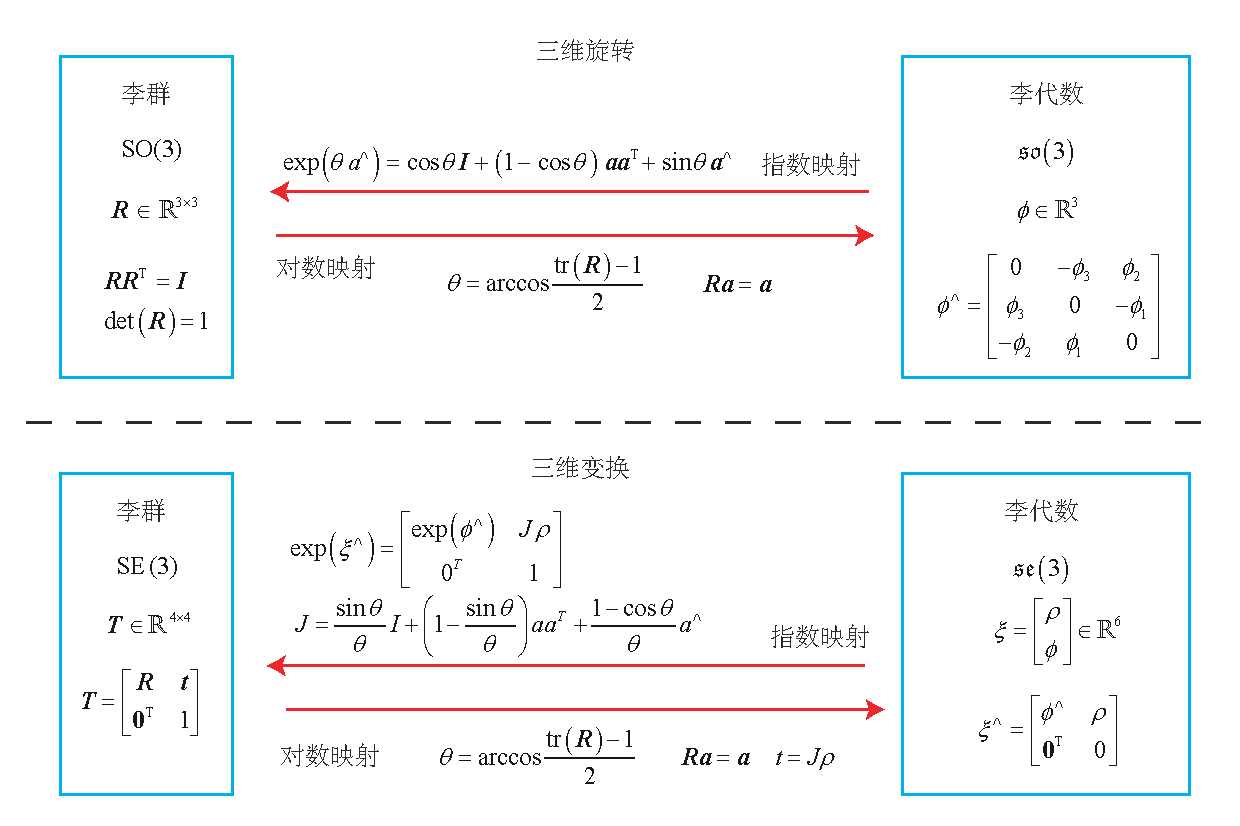
\includegraphics[width=1.0\textwidth]{lieGroup/liegroupandAlgebra.pdf}
    \caption{The correspondence between $\mathrm{SO}(3), \mathrm{SE}(3), \mathfrak{so}(3), \mathfrak{se}(3)$. }
    \label{fig:liegroupandAlgebra}
\end{figure}

\section{Lie Algebra Derivation and Perturbation Model}
\subsection{BCH Formula and its Approximation}
A major motivation for using Lie algebra is to do optimization. The derivative is a very necessary part of the optimization process (we will talk about it in detail in lecture~\ref{cpt:6}). Let's consider the problem below. Although we have already understood the relationship between Lie group and Lie algebra on $\mathrm{SO}(3)$ and $\mathrm{SE}(3)$, but what happens in $\mathfrak{so}(3)$ when two matrices are multiplied in $\mathrm{SO}(3)$? Conversely, when we add two vectors in $\mathfrak{so}(3)$, does $\mathrm{SO}(3)$ correspond to the product of the two matrices? If we write it out, it should be:
\[
\exp \left( {\boldsymbol{\phi}_1^\wedge } \right)\exp \left( {\boldsymbol{\phi}_2^\wedge}\right) = \exp \left( {{{\left( {{\boldsymbol{\phi} _1} + {\boldsymbol{\phi} _2}} \right)}^ \wedge }} \right) ?
\]

If $\boldsymbol{\phi}_1, \boldsymbol{\phi}_2$ are scalars, then this is obviously true; but here we calculate the exponential map of \textit{matrices} instead of scalars. In other words, we are studying whether the following formula holds:
\[
\ln \left( \exp \left( \mathbf{A} \right) \exp \left( \mathbf{B} \right) \right) = \mathbf{A} + \mathbf{B} \; ?
\]
for matrices. Unfortunately, this formula is not true in the matrix. The complete form of the product is given by the Baker-Campbell-Hausdorff formula (BCH formula)\footnote{ See \url{https://en.wikipedia.org/wiki/Baker-Campbell-Hausdorff\_formula}. }. Due to the complexity of its complete form, we only give the first few items of its expansion:
\begin{equation}
\ln \left( {\exp \left( \mathbf{A} \right)\exp \left( \mathbf{B} \right)} \right) = \mathbf{A} + \mathbf{B} + \frac{1}{2}\left[ {\mathbf{A}, \mathbf{B}} \right] + \frac{1}{{12}}\left[ {\mathbf{A},\left[ {\mathbf{A}, \mathbf{B}} \right]} \right] - \frac{1}{{12}}\left[ {\mathbf{B},\left[ {\mathbf{A} ,\mathbf{B}} \right]} \right] + \cdots
\end{equation}
where $[]$ is the Lie brackets. The BCH formula tells us that how to deal with the product of two matrices: they produce some extra Lie brackets compared with the scalar form. In particular, consider the case of $\mathrm{SO}(3)$ and $\ln { \left( {\exp \left( { \boldsymbol{\phi} _1^ \wedge } \right)\exp \left ( {\boldsymbol{\phi} _2^ \wedge } \right)} \right) ^ \vee }$, when $\boldsymbol{\phi_1}$ or $\boldsymbol{\phi_2}$ is small. Small items with more than quadratic can be  ignored when taking derivatives. At this time, BCH has a linear approximation\footnote{We are not going to do the detailed derivation of BCH approximation, see~\cite{Barfoot2016} if you are interested. }:
\begin{equation}
\ln { \left( {\exp \left( { \boldsymbol{\phi} _1^ \wedge } \right)\exp \left( {\boldsymbol{\phi} _2^ \wedge } \right)} \right ) ^ \vee } \approx \left\{
\begin{array}{l}
{\mathbf{J}_l}{\left( {{\boldsymbol{\phi} _2}} \right)^{ - 1}}{ \boldsymbol{\phi} _1} + {\boldsymbol{\phi} _2 } \quad \text{when} \ \boldsymbol{\phi}_1 \ \text{is a small amount},\\
{\mathbf{J}_r}{\left( {{\boldsymbol{\phi} _1}} \right)^{ - 1}}{\boldsymbol{\phi} _2} + {\boldsymbol{\phi} _1 } \quad \text{when} \  \boldsymbol{\phi}_2 \ \text{is a small amount}.
\end{array} \right.
\end{equation}

Take the first approximation as an example. This formula tells us that left multiplying a tiny rotation matrix $\mathbf{R}_1$ on a rotation matrix $\mathbf{R}_2$ (whose Lie algebra is $\boldsymbol{\phi}_1$ and $\boldsymbol{\phi}_2$, respectively), in $\mathfrak{so}(3)$ it can be approximated by adding a $\mathbf{J}_l \left( {\boldsymbol{\phi} _2} \right)^{ - 1} { \boldsymbol{\phi} _1}$ to the original Lie algebra $\boldsymbol{\phi}_2$.  Similarly, the second approximation describes the case where $\mathbf{R}_1$ is right multiplied by a small rotation. Therefore, under the BCH approximation, the Lie algebra is divided into a left-multiplying approximation and a right-multiplying approximation. We must pay attention to whether the left model or the right model is used in daily usage. This book takes the left multiplication as an example. The jacobian in our left model $\mathbf{J}_l$ is exactly the content of the form \eqref{eq:lieAlgebraJacobian}~:
\begin{equation}
{ \mathbf{J}_l} = \mathbf{J} = \frac{{\sin \theta }}{\theta } \mathbf{I} + \left( {1 - \frac{{\sin \theta } }{\theta }} \right) \mathbf{a} { \mathbf{a}^T} + \frac{{1 - \cos \theta }}{\theta }{ \mathbf{a} ^ \wedge}.
\end{equation}

Its inverse is:
\begin{equation}
\mathbf{J}_l^{ - 1} = \frac{\theta }{2}\cot \frac{\theta }{2} \mathbf{I} + \left( {1 - \frac{\theta } {2}\cot \frac{\theta }{2}} \right) \mathbf{a} {\mathbf{a}^T} - \frac{\theta }{2}{ \mathbf{ a}^ \wedge },
\end{equation}
when $\theta$ is not zero (in that case we take both $\mathbf{J}_{l}$ and its inverse as identity). To get the right jacobian we only need to take a negative sign for the argument:
\begin{equation}
\mathbf{J}_r(\boldsymbol{\phi}) =\mathbf{J}_l(-\boldsymbol{\phi}) .
\end{equation}

In this way, we've made it clear about the relationship between Lie group multiplication and Lie algebra addition.

For the convenience, we restate the meaning of the BCH approximation. Suppose we have a rotation $\mathbf{R}$, the corresponding Lie algebra is $\boldsymbol{\phi}$. We give it a small perturbation to the left, denoted as $\Delta \mathbf{R}$, and so that the corresponding Lie algebra is $\Delta \boldsymbol{\phi}$. Then, on Lie group, the result is $ \Delta \mathbf{R} \cdot \mathbf{R}$, and on the Lie algebra, according to the BCH approximation, it is $\mathbf{J}_l^{-1 } (\boldsymbol{\phi}) \Delta \boldsymbol{\phi} + \boldsymbol{\phi}$. Putting them together, we can simply write:
\begin{equation}
\exp \left( {\Delta { \boldsymbol{\phi} ^ \wedge }} \right)\exp \left( {{ \boldsymbol{\phi} ^ \wedge }} \right) = \exp \left( {{{\left( { \boldsymbol{\phi} + \mathbf{J}_l^{ - 1}\left( \boldsymbol{\phi} \right)\Delta \boldsymbol{\phi} } \right)} ^ \wedge }} \right).
\end{equation}

Conversely, if we do addition on Lie algebra by adding $\boldsymbol{\phi}$ with $\Delta \boldsymbol{\phi}$, we can approximate the multiplication on the Lie group as:
\begin{equation}
\exp \left( {{{\left( { \boldsymbol{\phi} + \Delta \boldsymbol{\phi} } \right)}^ \wedge }} \right) = \exp \left( {{{\left( {{ \mathbf{J}_l}\Delta \boldsymbol{\phi} } \right)}^ \wedge }} \right)\exp \left( {{ \boldsymbol{\phi} ^ \wedge }} \right) = \exp \left( {{\boldsymbol{\phi} ^ \wedge }} \right)\exp \left( {{{\left( {{\mathbf{J}_r}\Delta \boldsymbol{ \phi} } \right)}^ \wedge }} \right).
\end{equation}

This provides a theoretical basis for calculus on Lie algebra. Similarly, for $\mathrm{SE}(3)$, there is a similar BCH approximation:
\begin{equation}
\exp \left( {\Delta {\boldsymbol{\xi} ^ \wedge }} \right)\exp \left( {{ \boldsymbol{\xi} ^ \wedge }} \right) \approx \exp \left ( {{{\left( {{ \boldsymbol{\mathcal{J}}_l^{-1} }\Delta \boldsymbol{\xi} + \boldsymbol{\xi} } \right)}^ \wedge }} \right),
\end{equation}
\begin{equation}
\exp \left( {{ \boldsymbol{\xi} ^ \wedge }} \right) \exp \left( {\Delta {\boldsymbol{\xi} ^ \wedge }} \right) \approx \exp \left ( {{{\left( {{ \boldsymbol{\mathcal{J}}_r^{-1} }\Delta \boldsymbol{\xi} + \boldsymbol{\xi} } \right)}^ \wedge }} \right).
\end{equation}

Here the $\boldsymbol{\mathcal{J}}_l$ and $\boldsymbol{\mathcal{J}}_r$ are more complicated $6 \times 6$ matrices. Readers can find its detailed contents in~\cite{Barfoot2016}. Since we did not use these two jacobians matrices in the calculation (we will see in the next subsection), the exact form is omitted here.

\subsection{Derivative on $\mathrm{SO}(3)$}
Now let's talk about how to compute the derivation if our target function is related to a rotation or a transform, which has a powerful practical meaning since we usually have these functions to optimize in solving the SLAM problem. Assume we want to estimate a pose described by $\mathrm{SO}(3)$ or $\mathrm{SE}(3)$ elements. Our robot observes a point with the world coordinate $\mathbf{p}$ and generates an observation data $\mathbf{z}$, which can be written as:
\begin{equation}
\mathbf{z} = \mathbf{T} \mathbf{p} + \mathbf{w},
\end{equation}
where $\mathbf{w}$ is the noise (and is unknown). Because of the noise, the real observed data is not absolutely the same as the one we computed from the observation model, so we can calculate the error of predicted observation with the real one: 
\begin{equation}
\mathbf{e} = \mathbf{z} - \mathbf{T} \mathbf{p}.
\end{equation}

Suppose we have $N$ points in total, then we find a best $\mathbf{T}$ to make the error minimized: 
\begin{equation}
\mathop {\min }\limits_{\mathbf{T}} J(\mathbf{T} ) = \sum_{i=1}^{N} \left\| {\mathbf{z}_i - \mathbf{Tp}_i} \right\|^2_2.
\end{equation}

To solve such an optimization problem (which is a least square problem), we need to calculate the derivative of $J$ by $\mathbf{T}$. We leave the least square problem to the next section. Here we just want to clarify that we normally have some functions that have rotations or transforms as their variables. We have to adjust those rotations or transforms to find a better/best estimation. But, as we mentioned before, since $\mathrm{SO}(3)$ and $\mathrm{SE}(3)$ do not have a well-defined addition (they are just groups), so the derivatives cannot be defined in their common form. If we treat the $\mathbf{R}$ or $\mathbf{T}$ as common matrices, we have to introduce the constraints into our optimization. 

However, from the perspective of Lie algebra, since it consists of vectors, it has a good addition operation. Therefore, there are two ways to solve the problem of derivation using Lie algebra:

\begin{enumerate}
    \item Assume we add a infinitesimal amount on Lie algebra, then compute the change of the object function.
    \item Assume we multiply an infinitesimal perturbation on the Lie group left multiplication or right multiplication, use Lie algebra to describe the perturbation, and then compute the derivative on this perturbation. This is called as left perturbation or right perturbation model.
\end{enumerate}

The first method corresponds to the normal derivation model of the Lie algebra, and the second corresponds to the perturbation model. Let's discuss the similarities and differences between these two approaches.

\subsection{Derivative Model}
First, consider the situation on $\mathrm{SO}(3)$. Suppose we rotate a space point $\mathbf{p}$ and get $\mathbf{R} \mathbf{p}$. To calculate the derivative of the point coordinates by the rotation, we informally write it as \footnote{Please note that the derivative cannot be defined by matrix differentiation. Here we just write it for convenience. }:
\[
\frac{{\partial \left( {\mathbf{Rp}} \right)}}{{\partial \mathbf{R}}}.
\]
Since $\mathrm{SO}(3)$ has no addition operator, it cannot be calculated by the common derivative definition. Let the Lie algebra corresponding to $\mathbf{R}$ be $\boldsymbol{\phi}$, and we will calculate instead of the common derivative:\footnote{Strictly speaking, in matrix differentiation, we can only compute the derivative of a row vector to a column vector, whose result is a matrix. However, in this book, we write the derivative of the column vector to the column vector for convenience. The reader can think that the numerator is transposed first, and after the computation, the final result is also transposed (see appendix~\ref{cpt:app-B} for details). This makes the formula look simple; otherwise, we have to add a transpose to each equation. In this sense, we can use equations like $\mathrm{d}(\mathbf{Ax})/\mathrm{d}\mathbf{x} = \mathbf{A}$. }:
\[ \frac{{\partial \left( {\exp \left( \boldsymbol{\phi} ^ \wedge \right) \mathbf{p}} \right)}}{{\partial \boldsymbol{\phi} }}. \]

%\clearpage
According to the definition of the derivative, we have:
\begin{align*}
\frac{{\partial \left( {\exp \left( {{ \boldsymbol{\phi} ^ \wedge }} \right) \mathbf{p}} \right)}}{{\partial \boldsymbol{\phi} }} &= \mathop {\lim }\limits_{\delta \boldsymbol{\phi}  \to \mathbf{0}} \frac{{\exp \left( {{{\left( {\boldsymbol{\phi}  + \delta \boldsymbol{\phi} } \right)}^ \wedge }} \right) \mathbf{p} - \exp \left( {{\boldsymbol{\phi} ^ \wedge }} \right)\mathbf{p}}}{{\delta \boldsymbol{\phi} }}\\
& = \mathop {\lim }\limits_{\delta \boldsymbol{\phi}  \to \mathbf{0}} \frac{{\exp \left( {{{\left( {{\mathbf{J}_l}\delta \boldsymbol{\phi} } \right)}^ \wedge }} \right)\exp \left( {{\boldsymbol{\phi} ^ \wedge }} \right) \mathbf{p} - \exp \left( {{\boldsymbol{\phi} ^ \wedge }} \right) \mathbf{p}}}{{\delta \boldsymbol{\phi} }}\\
&= \mathop {\lim }\limits_{\delta \boldsymbol{\phi}  \to \mathbf{0}} \frac{{\left( { \mathbf{I} + {{\left( {{ \mathbf{J}_l}\delta \boldsymbol{\phi} } \right)}^ \wedge }} \right)\exp \left( {{\boldsymbol{\phi} ^ \wedge }} \right) \mathbf{p} - \exp \left( {{\boldsymbol{\phi} ^ \wedge }} \right)\mathbf{p}}}{{\delta \boldsymbol{\phi} }}\\
&= \mathop {\lim }\limits_{\delta \boldsymbol{\phi}  \to \mathbf{0}} \frac{{{{\left( {{\mathbf{J}_l}\delta \boldsymbol{\phi} } \right)}^ \wedge }\exp \left( {{\boldsymbol{\phi} ^ \wedge }} \right)\mathbf{p}}}{{\delta \boldsymbol{\phi} }}\\
&= \mathop {\lim }\limits_{\delta \boldsymbol{\phi}  \to \mathbf{0}} \frac{{ - {{\left( {\exp \left( {{\boldsymbol{\phi} ^ \wedge }} \right)\mathbf{p}} \right)}^ \wedge }{\mathbf{J}_l}\delta \boldsymbol{\phi} }}{{\delta \boldsymbol{\phi}}} =  - {\left( {\mathbf{Rp}} \right)^ \wedge }{\mathbf{J}_l}.
\end{align*}

The second line is BCH approximation. The third line is Taylor's approximation after throwing the high-order terms (but we still write the equal sign here because the limit is taken). The fourth to the fifth line treat the skew-symmetric symbol as a cross-product so that $\mathbf{a} \times \mathbf{b} = -\mathbf{b} \times \mathbf{a}$. Thus, we compute the derivative of the rotated point relative to the addition in Lie algebra:
\begin{equation}
\frac{{\partial \left( { \mathbf{Rp}} \right)}}{{\partial \boldsymbol{\phi} }} = {\left( { - \mathbf{Rp}} \right)^ \wedge }{\mathbf{J}_l}.
\end{equation}

However, since there is still a very complicated form of $\mathbf{J}_l$, we don't want to calculate it. The perturbation model described below provides a more straightforward way to compute derivatives.

\subsection{Perturbation Model}
Another way to do this is to perturb $\mathbf{R}$ by $\Delta \mathbf{R}$ and see the change of the result relative to the disturbance. This disturbance can be multiplied on the left or on the right. The final result will be slightly different. Let's take the left perturbation as an example. Let the left perturbation $\Delta \mathbf{R}$ correspond to the Lie algebra as $\boldsymbol{\varphi}$. Then, for $\boldsymbol{\varphi}$, that is:
\begin{equation}
\frac{{\partial \left( {\mathbf{Rp}} \right)}}{{\partial \boldsymbol{\varphi} }} = \mathop {\lim }\limits_{\boldsymbol{\varphi}  \to \mathbf{0}} \frac{{\exp \left( {{\boldsymbol{\varphi} ^ \wedge }} \right)\exp \left( {{\boldsymbol{\phi} ^ \wedge }} \right)\mathbf{p} - \exp \left( {{\boldsymbol{\phi} ^ \wedge }} \right)\mathbf{p}}}{\boldsymbol{\varphi} }.
\end{equation}

The derivation of this formula is simpler than the above:
\begin{align*}
\frac{{\partial \left( {\mathbf{Rp}} \right)}}{{\partial \boldsymbol{\varphi} }} &= \mathop {\lim }\limits_{\boldsymbol{\varphi}  \to \mathbf{0}} \frac{{\exp \left( {{\boldsymbol{\varphi} ^ \wedge }} \right)\exp \left( {{\boldsymbol{\phi} ^ \wedge }} \right)\mathbf{p} - \exp \left( {{\boldsymbol{\phi} ^ \wedge }} \right)\mathbf{p}}}{ \boldsymbol{\varphi} }\\
&= \mathop {\lim }\limits_{\boldsymbol{\varphi } \to \mathbf{0}} \frac{{\left( {\mathbf{I} + {\boldsymbol{\varphi }^ \wedge }} \right)\exp \left( {{\boldsymbol{\phi} ^ \wedge }} \right)\mathbf{p} - \exp \left( {{\boldsymbol{\phi} ^ \wedge }} \right)\mathbf{p}}}{\boldsymbol{\varphi} }\\
&= \mathop {\lim }\limits_{\boldsymbol{\varphi}  \to \mathbf{0}} \frac{{{\boldsymbol{\varphi} ^ \wedge }\mathbf{Rp}}}{\boldsymbol{\varphi} } = \mathop {\lim }\limits_{\boldsymbol{\varphi}  \to \mathbf{0}} \frac{{ - {{\left( \mathbf{Rp} \right)}^ \wedge }\boldsymbol{\varphi} }}{\boldsymbol{\varphi} } =  - {\left( \mathbf{Rp} \right)^ \wedge }.
\end{align*}

It can be seen that the calculation of a Jacobian $\mathbf{J}_l$ is omitted compared to Lie algebra's direct derivation. This makes the perturbation model more practical. Please keep in mind the derivative here since we will use it in the pose estimation sections.


\subsection{Derivative on $\mathrm{SE}(3)$}
\label{sec:se3-diff}
Finally, we give the perturbation model on $\mathrm{SE}(3)$, and skip the derivative model. Suppose a point $\mathbf{p}$ is transformed by $\mathbf{T}$ (corresponding to Lie algebra $\boldsymbol{\xi}$), and the result is $\mathbf{Tp}$\footnote{Please note that to make multiplication make sense, $\mathbf{p}$ must use homogeneous coordinates. }. Now, give $\mathbf{T}$ a left perturbation $\Delta \mathbf{T} = \exp \left( \delta \boldsymbol{\xi}^\wedge \right)$, whose Lie algebra is $\delta \boldsymbol{\xi} = [\delta \boldsymbol{\rho}, \delta \boldsymbol{\phi}]^T$, then:

\begin{align*}
\frac{{\partial \left( \mathbf{Tp} \right)}}{{\partial \delta \boldsymbol{\xi}}} &= \mathop {\lim }\limits_{\delta \boldsymbol{\xi}  \to \mathbf{0}} \frac{{\exp \left( {\delta {\boldsymbol{\xi} ^ \wedge }} \right)\exp \left( {{\boldsymbol{\xi} ^ \wedge }} \right) \mathbf{p} - \exp \left( {{\boldsymbol{\xi} ^ \wedge }} \right) \mathbf{p} }}{{\delta \boldsymbol{\xi} }}\\
&= \mathop {\lim }\limits_{\delta \boldsymbol{\xi}  \to \mathbf{0}} \frac{{\left( { \mathbf{I} + \delta {\boldsymbol{\xi} ^ \wedge }} \right)\exp \left( {{\boldsymbol{\xi} ^ \wedge }} \right) \mathbf{p} - \exp \left( {{\boldsymbol{\xi} ^ \wedge }} \right) \mathbf{p} }}{{\delta {\boldsymbol{\xi} }}}\\
&= \mathop {\lim }\limits_{\delta \boldsymbol{\xi}  \to \mathbf{0}} \frac{{\delta {\boldsymbol{\xi} ^ \wedge }\exp \left( {{\boldsymbol{\xi} ^ \wedge }} \right) \mathbf{p}}}{{\delta {\boldsymbol{\xi} }}}\\
&= \mathop {\lim }\limits_{\delta \boldsymbol{\xi}  \to \mathbf{0}} 
\frac{{\left[ {\begin{array}{*{20}{c}}
                {\delta { \boldsymbol{\phi} ^ \wedge }}&{\delta {\boldsymbol{\rho} }}\\
                {{\mathbf{0}^T}}&0
        \end{array}} \right]\left[ {\begin{array}{*{20}{c}}
                {\mathbf{Rp} + \mathbf{t}}\\
                1
        \end{array}} \right]}}{{\delta {\boldsymbol{\xi} }}}\\
&= \mathop {\lim }\limits_{\delta \boldsymbol{\xi}  \to \mathbf{0}} \frac{{\left[ {\begin{array}{*{20}{c}}
                {\delta {\boldsymbol{\phi} ^ \wedge }\left( {\mathbf{Rp} + \mathbf{t}} \right) + \delta {\boldsymbol{\rho} }}\\
                \mathbf{0}^T
        \end{array}} \right]}}{[\delta\boldsymbol{\rho},\delta \boldsymbol{\phi}]^T} = \left[ {\begin{array}{*{20}{c}}
        \mathbf{I} & { - {{\left( {\mathbf{Rp} + \mathbf{t}} \right)}^ \wedge }} \\
        {{\mathbf{0}}}^T & \mathbf{0}^T
\end{array}} \right] \buildrel \Delta \over = {\left( \mathbf{Tp} \right)^ \odot }.
\end{align*}

We define the final result as an operator $^\odot$\footnote{I will read it as ``Duang'', like a stone falling into a well.}, which transforms a spatial point of homogeneous coordinates into a matrix of $4 \times 6$. This equation requires a little explanation about matrix differentiation. Assuming that $\mathbf{a}, \mathbf{b}, \mathbf{x}, \mathbf{y}$ are column vectors, then in our book, there are following rules:
\begin{equation}
\frac{\mathrm{\mathrm{d}}\begin{bmatrix}
    \mathbf{a}\\
    \mathbf{b}
    \end{bmatrix}}{{\mathrm{d} \begin{bmatrix}
        \mathbf{x}\\
        \mathbf{y}
        \end{bmatrix}}} = {\left( \frac{\mathrm{d}[\mathbf{a},\mathbf{b}]^T}{{\mathrm{d}\begin{bmatrix}
            \mathbf{x}\\
            \mathbf{y}
            \end{bmatrix}}} \right)^T} = {{\begin{bmatrix}
        {\frac{{\mathrm{d}\mathbf{a}}}{{\mathrm{d}\mathbf{x}}}}&{\frac{{\mathrm{d}\mathbf{b}}}{{\mathrm{d}\mathbf{x}}}}\\
        {\frac{{\mathrm{d}\mathbf{a}}}{{\mathrm{d}\mathbf{y}}}}&{\frac{{\mathrm{d}\mathbf{b}}}{{\mathrm{d}\mathbf{y}}}}
        \end{bmatrix}} ^T} = {\begin{bmatrix}
    {\frac{{\mathrm{d}\mathbf{a}}}{{\mathrm{d}\mathbf{x}}}}&{\frac{{\mathrm{d}\mathbf{a}}}{{\mathrm{d}\mathbf{y}}}}\\
    {\frac{{\mathrm{d}\mathbf{b}}}{{\mathrm{d}\mathbf{x}}}}&{\frac{{\mathrm{d}\mathbf{b}}}{{\mathrm{d}\mathbf{y}}}}
    \end{bmatrix}}
\end{equation}
Substituting this into the last line, you can get the final result. So far, we have introduced the differential operation on Lie group Lie algebra. In the following chapters, we will apply this knowledge to solve practical problems. 

\section{Practice: Sophus}
\subsection{Basic Usage of Sophus}
We have introduced the basic knowledge of Lie algebra, and now it is time to consolidate what we have learned through practical exercises. Let's discuss how to manipulate Lie algebra in a program. In lecture 3, we saw that \textit{Eigen} provided geometry modules but did not support Lie algebra. A better Lie algebra library is the Sophus library maintained by Strasdat (\url{https://github.com/strasdat/Sophus})\footnote{Sophus Lie first proposed the Lie algebra. The library is named after him.}. The Sophus library supports $\mathrm{SO}(3)$ and $\mathrm{SE}(3)$, which are mainly discussed in this chapter. In addition, it also contains two-dimensional motion $\mathrm{SO}(2), \mathrm{SE} (2) $ and the similar transformation of $\mathrm{Sim}(3)$. It is developed directly on top of \textit{Eigen}, and we don't need to install additional dependencies. Readers can get Sophus directly from GitHub, or the Sophus source code is also available in our book's code directory ``slambook2/3rdparty''. For historical reasons, earlier versions of Sophus only provided double-precision Lie group/Lie algebra classes. Subsequent versions have been rewritten as template classes so that different precision of Lie group/Lie algebra can be used in the Sophus from the template class. But, at the same time, it increases the difficulty of use. In the second edition of this book, we use the Sophus library with templates. The Sophus provided in the 3rdparty of this book is the template version, which should have been copied to your computer during the downloading process. Sophus itself is also a CMake project. Presumably, you already know how to compile the CMake project, so I won't go into details here. The Sophus library only needs to be compiled, no need to install it.

Let's demonstrate the $\mathrm{SO}(3)$ and $\mathrm{SE}(3)$ operations in the Sophus library:

\begin{lstlisting}[language=c++,caption=slambook/ch4/useSophus.cpp]
#include <iostream>
#include <cmath>
#include <Eigen/Core>
#include <Eigen/Geometry>
#include "sophus/se3.hpp"

using namespace std;
using namespace Eigen;

/// This program demonstrates the basic usage of Sophus
int main(int argc, char **argv) {
    // Rotation matrix with 90 degrees along Z axis
    Matrix3d R = AngleAxisd(M_PI / 2, Vector3d(0, 0, 1)).toRotationMatrix();
    // or quaternion
    Quaterniond q(R);
    Sophus::SO3d SO3_R(R);              // Sophus::SO3d can be constructed from rotation matrix
    Sophus::SO3d SO3_q(q);              // or quaternion
    // they are equivalent of course
    cout << "SO(3) from matrix:\n" << SO3_R.matrix() << endl;
    cout << "SO(3) from quaternion:\n" << SO3_q.matrix() << endl;
    cout << "they are equal" << endl;
    
    // Use logarithmic map to get the Lie algebra
    Vector3d so3 = SO3_R.log();
    cout << "so3 = " << so3.transpose() << endl;
    // hat is from vector to skew-symmetric matrix
    cout << "so3 hat=\n" << Sophus::SO3d::hat(so3) << endl;
    // inversely from matrix to vector
    cout << "so3 hat vee= " << Sophus::SO3d::vee(Sophus::SO3d::hat(so3)).transpose() << endl;
    
    // update by perturbation model
    Vector3d update_so3(1e-4, 0, 0); // this is a small update
    Sophus::SO3d SO3_updated = Sophus::SO3d::exp(update_so3) * SO3_R;
    cout << "SO3 updated = \n" << SO3_updated.matrix() << endl;
    
    cout << "*******************************" << endl;
    // Similar for SE(3)
    Vector3d t(1, 0, 0);                 // translation 1 along X
    Sophus::SE3d SE3_Rt(R, t);           // construction SE3 from R,t
    Sophus::SE3d SE3_qt(q, t);           // or q,t
    cout << "SE3 from R,t= \n" << SE3_Rt.matrix() << endl;
    cout << "SE3 from q,t= \n" << SE3_qt.matrix() << endl;
    // Lie Algebra is 6d vector, we give a typedef
    typedef Eigen::Matrix<double, 6, 1> Vector6d;
    Vector6d se3 = SE3_Rt.log();
    cout << "se3 = " << se3.transpose() << endl;
    // The output shows Sophus puts the translation at first in se(3), then rotation.
    // Save as SO(3) wehave hat and vee
    cout << "se3 hat = \n" << Sophus::SE3d::hat(se3) << endl;
    cout << "se3 hat vee = " << Sophus::SE3d::vee(Sophus::SE3d::hat(se3)).transpose() << endl;
    
    // Finally the update
    Vector6d update_se3; 
    update_se3.setZero();
    update_se3(0, 0) = 1e-4d;
    Sophus::SE3d SE3_updated = Sophus::SE3d::exp(update_se3) * SE3_Rt;
    cout << "SE3 updated = " << endl << SE3_updated.matrix() << endl;
    
    return 0;
}
\end{lstlisting}

The demo is divided into two parts. The first half introduces the operation on $\mathrm{SO}(3)$, and the second half is $\mathrm{SE}(3)$. We demonstrate how to construct $\mathrm{SO}(3), \mathrm{SE}(3)$ objects as well as the exponential/logarithm mapping. And then, we update the lie group elements when we know the updated amount. If the reader has a good understanding of this lecture's content, then this program should not be difficult for you. To compile it, add the following lines to ``CMakeLists.txt'':

\begin{lstlisting}[caption=slambook2/ch4/useSophus/CMakeLists.txt]
# we use find_package to make CMake find sophus
find_package( Sophus REQUIRED )
include_directories( ${Sophus_INCLUDE_DIRS} ) # sohpus is header only

add_executable( useSophus useSophus.cpp )
\end{lstlisting}


The \textit{find\_package} is a command provided by CMake to find the header and library files of a library. If CMake can find it, it will provide the variables for the directory where the header and library files are located. In the example of Sophus, it is Sophus\_INCLUDE\_DIRS. The template-based Sophus library, like \textit{Eigen}, contains only header files and no source files. Based on them, we can introduce the Sophus library into our own CMake project. Readers are asked to see the output of this program on their own, consistent with our previous derivation.

\subsection{Example: Evaluating the Trajectory}
In practical engineering, we often need to evaluate the difference between the estimated trajectory of an algorithm and the real trajectory to evaluate the algorithm's accuracy. The real (or ground-truth) trajectory is often obtained by some higher precision systems, and the estimated one is calculated by the algorithm to be evaluated. In the last lecture, we demonstrated how to display a trajectory stored in a file. In this section, we will consider how to calculate the error of two trajectories. Consider an estimated trajectory $\mathbf{T}_{\mathrm{esti}, i}$ and the real trajectory $\mathbf{T}_{\mathrm{gt},i}$, where $i=1,\cdots, N$; then we can define some error indicators to describe the difference between them.

There are many kinds of error indicators. The common used one is \textit{absolute trajectory error}, which is like:
\begin{equation}
\mathrm{ATE}_{\mathrm{all}} = \sqrt{ \frac{1}{N} \sum_{i=1}^N \| \log( \mathbf{T}_{\mathrm{gt },i}^{-1} \mathbf{T}_{\mathrm{esti},i} )^{\vee} \|_2^2},
\end{equation}
This is actually the root-mean-squared error (RMSE) for each pose in Lie algebra. This error can describe both the rotation and translation errors. At the same time, some literature only consider the translation error~\cite{Sturm2012}, so we can define the \textit{average translational error}:
\begin{equation}
\mathrm{ATE}_{\mathrm{trans}} = \sqrt{ \frac{1}{N} \sum_{i=1}^N \| \mathrm{trans}( \mathbf{T}_{\mathrm{gt},i}^{-1} \mathbf{T}_{\mathrm{esti},i} ) \|_2^2},
\end{equation}
where the function ``$\mathrm{trans}$'' represents the translation of the internal variables of the parentheses. From the perspective of the entire trajectory, if we have a rotation error, it will also affect the subsequent translation. So both indicators are applicable in practice.

In addition to this, relative error indicators can also be defined. For example, consider the movement from $i$ to the time of $i+\Delta t$, then the relative pose error (RPE) can be defined as:
\begin{equation}
\mathrm{RPE}_{\mathrm{all}} = \sqrt{ \frac{1}{N-\Delta t} \sum_{i=1}^{N-\Delta t} \| \log \left ( \left(\mathbf{T}_{\mathrm{gt},i}^{-1} \mathbf{T}_{\mathrm{gt},i+\Delta t} )\right)^{-1 } \left(\mathbf{T}_{\mathrm{esti},i}^{-1} \mathbf{T}_{\mathrm{esti},i+\Delta t}\right)\right)^{ \vee} \|_2^2},
\end{equation}
Similarly, you can only take the translation part:
\begin{equation}
\mathrm{RPE}_{\mathrm{trans}} = \sqrt{ \frac{1}{N-\Delta t} \sum_{i=1}^{N-\Delta t} \| \mathrm{trans } \left( \left(\mathbf{T}_{\mathrm{gt},i}^{-1} \mathbf{T}_{\mathrm{gt},i+\Delta t} )\right)^ {-1} \left(\mathbf{T}_{\mathrm{esti},i}^{-1} \mathbf{T}_{\mathrm{esti},i+\Delta t}\right)\right ) \|_2^2}.
\end{equation}

This part of the calculation is easy to implement with the Sophus library. Below we demonstrate the calculation of the absolute trajectory error. In this example, we have two trajectories: ``groundtruth.txt'' and ``estimated.txt''. The following code will read the two trajectories, calculate the error, and display it in a 3D window. For the sake of brevity, the code for the trajectory plotting has been omitted, as we have done similar work in the previous section.
    
\begin{lstlisting}[language=c++,caption=slambook/ch4/example/trajectoryError.cpp (part)]
#include <iostream>
#include <fstream>
#include <unistd.h>
#include <pangolin/pangolin.h>
#include <sophus/se3.hpp>

using namespace Sophus;
using namespace std;

string groundtruth_file = "./example/groundtruth.txt";
string estimated_file = "./example/estimated.txt";

typedef vector<Sophus::SE3d, Eigen::aligned_allocator<Sophus::SE3d>> TrajectoryType;

void DrawTrajectory(const TrajectoryType &gt, const TrajectoryType &esti);

TrajectoryType ReadTrajectory(const string &path);

int main(int argc, char **argv) {
    TrajectoryType groundtruth = ReadTrajectory(groundtruth_file);
    TrajectoryType estimated = ReadTrajectory(estimated_file);
    assert(!groundtruth.empty() && !estimated.empty());
    assert(groundtruth.size() == estimated.size());
    
    // compute rmse
    double rmse = 0;
    for (size_t i = 0; i < estimated.size(); i++) {
        Sophus::SE3d p1 = estimated[i], p2 = groundtruth[i];
        double error = (p2.inverse() * p1).log().norm();
        rmse += error * error;
    }
    rmse = rmse / double(estimated.size());
    rmse = sqrt(rmse);
    cout << "RMSE = " << rmse << endl;
    
    DrawTrajectory(groundtruth, estimated);
    return 0;
}

TrajectoryType ReadTrajectory(const string &path) {
    ifstream fin(path);
    TrajectoryType trajectory;
    if (!fin) {
        cerr << "trajectory " << path << " not found." << endl;
        return trajectory;
    }
    
    while (!fin.eof()) {
        double time, tx, ty, tz, qx, qy, qz, qw;
        fin >> time >> tx >> ty >> tz >> qx >> qy >> qz >> qw;
        Sophus::SE3d p1(Eigen::Quaterniond(qx, qy, qz, qw), Eigen::Vector3d(tx, ty, tz));
        trajectory.push_back(p1);
    }
    return trajectory;
}
\end{lstlisting}

The result of this program is 2.207, and the image is shown as \autoref{fig:trajectory-compare}. You can also try to remove the rotating part and only calculates the error of the translation part. In fact, in this example, we have helped the reader to do some pre-processing tasks, including time alignment of the trajectory and external parameter estimation. These contents have not been mentioned yet, and we will talk about them in the future.

\begin{figure}[!ht]
    \centering
    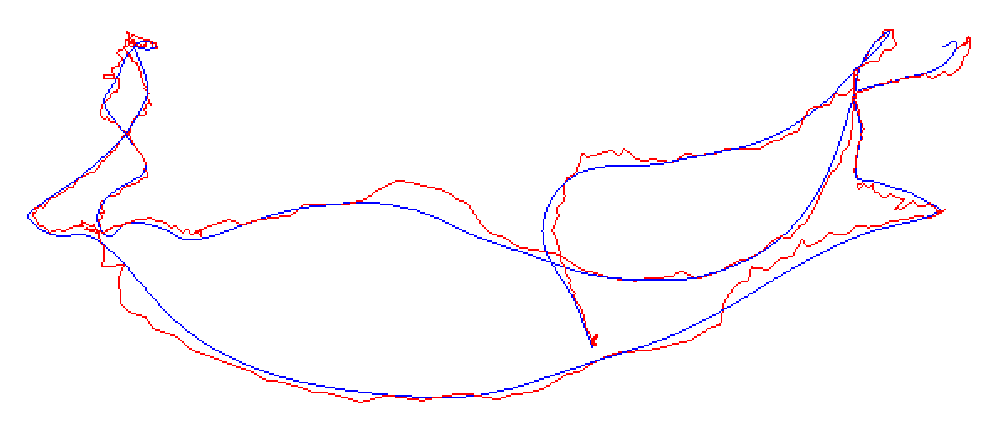
\includegraphics[width=1.0\textwidth]{lieGroup/trajectory-compare.pdf}
    \caption{Calculates the error between the estimated trajectory and the real trajectory. }
    \label{fig:trajectory-compare}
\end{figure}

\section{Similar Transform Group and Its Lie Algebra}
Finally, we would like to mention the similar transform group $\mathrm{Sim}(3)$ used in monocular vision, and the corresponding Lie algebra $\mathfrak{sim}(3)$. If you are only interested in stereo or RGB-D SLAM, you can skip this section.

We have already introduced the concept of scale ambiguity. If $\mathrm{SE}(3)$ is used in the monocular SLAM to represent the pose, then the scale in the entire SLAM process will change due to scale uncertainty and scale drift, which is what $\mathrm{SE}(3) $ not reflects. Therefore, in the case of monocular SLAM, we generally express the scale factor explicitly. In mathematical terms, for the point $\mathbf{p}$ in space, a \textit{similar transformation} is passed in the camera coordinate system instead of the Euclidean transformation:
\begin{equation}
\mathbf{p}' = \left[ {\begin{array}{*{20}{c}}
    {s\mathbf{R}}&\mathbf{t}\\
    {{\mathbf{0}^T}}&1
    \end{array}} \right] \mathbf{p}
= s\mathbf{R} \mathbf{p} + \mathbf{t}.
\end{equation}
In the similarity transformation, we express the scale as $s$. It also acts on top of the three coordinates of $\mathbf{p}$ and scales $\mathbf{p}$ once. Similar to $\mathrm{SO}(3)$, $\mathrm{SE}(3)$, the similarity transform also forms a group on matrix multiplication, called the similarity transform group $\mathrm{Sim}(3)$:
\begin{equation}
\mathrm{Sim}(3) = \left\{ { \mathbf{S} = \left[ {\begin{array}{*{20}{c}}
        {s\mathbf{R}}& \mathbf{t}\\
        {{\mathbf{0}^T}}&1
        \end{array}} \right] \in {\mathbb{R}^{4 \times 4}}} \right\}.
\end{equation}

Similarly, $\mathrm{Sim}(3)$ also has corresponding Lie algebra, exponential mapping, logarithmic mapping, and so on. The Lie algebra $\mathfrak{sim}(3)$ element is a 7-dimensional vector $\boldsymbol{\zeta}$. Its first 6 dimensions are the same as $\mathfrak{se}(3)$, followed by a $\sigma$ to denote the scale.

\begin{equation}
\mathfrak{sim} \left( 3 \right) = \left\{ { \boldsymbol{\zeta} | \boldsymbol{\zeta} = \left[ \begin{array}{l}
    \boldsymbol{\rho} \\
    \boldsymbol{\phi} \\
    \sigma
    \end{array} \right] \in { \mathbb{R}^7},{ \boldsymbol{\zeta} ^ \wedge } = \left[ {\begin{array}{*{20}{c}}
        {\sigma \mathbf{I} + {\boldsymbol{\phi} ^ \wedge }}&\boldsymbol{\rho} \\
        {{\mathbf{0}^T}}&0
        \end{array}} \right] \in {\mathbb{R}^{4 \times 4}}} \right\}.
\end{equation}

It has an additional $\sigma$ compared with $\mathfrak{se}(3)$. The $\mathrm{Sim}(3)$ and $\mathfrak{sim}(3)$ are still associated with exponential maps and logarithm maps. The exponential mapping is:

\begin{equation}
\exp \left( {{ \boldsymbol{\zeta} ^ \wedge }} \right) = \left[ {\begin{array}{*{20}{c}}
    {{\mathrm{e}^\sigma }\exp \left( {{ \boldsymbol{\phi} ^ \wedge }} \right)}&{ \mathbf{J}_s \boldsymbol{\rho} }\\
    {{\mathbf{0}^T}}&1
    \end{array}} \right],
\end{equation}
where $\mathbf{J}_s$ is:
\begin{align*}
%\begin{array}{ll}
{ \mathbf{J}_s} =& \frac{{{\mathrm{e}^\sigma } - 1}}{\sigma } \mathbf{I} + \frac{ \sigma {{\mathrm{e} ^\sigma }\sin \theta + \left( {1 - {\mathrm{e}^\sigma }\cos \theta } \right)\theta }}{{{\sigma ^2} + {\theta ^ 2}}}{\mathbf{a}^ \wedge }\\
&+ \left( {\frac{{{\mathrm{e}^\sigma } - 1}}{\sigma } - \frac{{\left( {{\mathrm{e}^\sigma }\cos \theta - 1} \right)\sigma + ({\mathrm{e}^\sigma }\sin \theta )\theta }}{{{\sigma ^2} + {\theta ^2}}}} \right ){\mathbf{a}^ \wedge }{\mathbf{a}^ \wedge }.
%\end{array}
\end{align*}

Through exponential mapping, we can find the relationship between Lie algebra and Lie group. For the Lie algebra $\boldsymbol{\zeta}$, its correspondence with the Lie group is:
\begin{equation}
s=\mathrm{e}^\sigma, \; \mathbf{R} = \exp( \boldsymbol{\phi} ^\wedge), \; \mathbf{t} = \mathbf{J}_s \boldsymbol{ \rho}.
\end{equation}

The rotation is consistent with $\mathrm{SO}(3)$. In the translation part, we need to multiply a Jacobian $\boldsymbol{\mathcal{J}}$ in $\mathfrak{se}(3)$, and the similarly transformed Jacobi is more complicated. For the scale factor, you can see that $s$ in the Lie group is the exponential function of $\sigma$ in the Lie algebra.

The BCH approximation of $\mathrm{Sim}(3)$ is similar to $\mathrm{SE}(3)$. We can discuss a derivative of $\mathbf{S}$ after a similar transformation of $\mathbf{S} \mathbf{p}$ relative to $\mathbf{S}$. Similarly, there are two ways of the differential model and perturbation model, and the perturbation model is the simpler one. We omit the derivation process and directly give the results of the perturbation model. Let $\mathbf{S} \mathbf{p}$ a small perturbation $\exp( \boldsymbol{\zeta} ^\wedge )$ on the left and ask for $\mathbf{S} \mathbf{p}$ The derivative of the disturbance. Since $\mathbf{S} \mathbf{p}$ is a 4-dimensional homogeneous coordinate, $\boldsymbol{\zeta}$ is a 7-dimensional vector, which should have $4 \times 7$ Jacobian. For convenience, remember the first three-dimensional composition vector $\mathbf{q}$ of $\mathbf{Sp}$, then:

\begin{equation}
\frac{{\partial \mathbf{Sp}}}{{\partial \boldsymbol{\zeta} }} = \left[ {\begin{array}{*{20}{c}}
    \mathbf{I} &{ - {\mathbf{q}^ \wedge }}& \mathbf{q} \\
    {{\mathbf{0}^T}} & {{ \mathbf{0}^T}}&0
    \end{array}} \right].
\end{equation}

We will end here about the contents of $\mathrm{Sim}(3)$. For more detailed information on $\mathrm{Sim}(3)$, please refer to the literature~\cite{Strasdat2012a}.

\section{Summary}
This lecture introduces Lie group $\mathrm{SO}(3)$ and $\mathrm{SE}(3)$, and their corresponding Lie algebras $\mathfrak{so}(3)$ and $\mathfrak{se }(3)$. We introduce the expression and transformation of poses on them, and then through the linear approximation of BCH, we can perturb and predict the pose. This lays the theoretical foundation for optimizing the pose afterward because we need to adjust the estimate of a certain pose frequently to reduce the corresponding error. Only after we have figured out how to adjust and update the pose can we continue to the next step.

The content of this lecture may be more theoretical. After all, it is not as good as computer vision. Compared to the mathematics textbooks that explain Lie group Lie algebra, since we only care about practical content, the process is very streamlined, and the speed is relatively fast. The reader must understand the content of this lecture, which is the basis for solving many subsequent problems, especially the pose estimation part.

It should be mentioned that in addition to the Lie algebra, the rotation can also be expressed by quaternion, Euler angle, etc., but the subsequent processing is troublesome. In practice, you can also use $\mathrm{SO}(3)$ plus a translation instead of $\mathrm{SE}(3)$ to avoid some Jacobian calculations.

\section*{Exercises}
\begin{enumerate}
    \item Verify $\mathrm{SO}(3)$, $\mathrm{SE}(3)$, and $\mathrm{Sim}(3)$ are groups on matrix multiplication.
    \item Verify that $( \mathbb{R}^3, \mathbb{R}, \times )$ constitutes a Lie algebra.
    \item Verify that $\mathfrak{so}(3)$ and $\mathfrak{se}(3)$ satisfy the requirements of Lie algebra.
    \item Verify the properties (4.20) and (4.21).
    \item Show that: \[
    \mathbf{R} \mathbf{p}^\wedge \mathbf{R}^T = (\mathbf{Rp})^\wedge .\]
    \item Show that: \[
    \mathbf{R} \exp( \mathbf{p}^\wedge) \mathbf{R}^T = \exp( (\mathbf{Rp})^\wedge ).\] This is called the \textit{adjoint} property on $\mathrm{SO}(3)$. Similarly, there is an adjoint property on $\mathrm{SE}(3)$:
    \begin{equation}
    \mathbf{T} \exp(\boldsymbol{\xi}^\wedge)\mathbf{T}^{-1} = \exp \left( \left( \mathrm{Ad}(\mathbf{T}) \boldsymbol{\xi} \right) ^\wedge \right),
    \end{equation}
    where
    \begin{equation}
    \label{eq:adjSE3}
    \mathrm{Ad} ( \mathbf{T} ) = \left[ {\begin{array}{*{20}{c}}
        \mathbf{R} &{{ \mathbf{t} ^ \wedge } \mathbf{R} }\\
        \mathbf{0} & \mathbf{R}
        \end{array}} \right].
    \end{equation}
    \item Follow the derivation of the left perturbation and derives the derivatives of $\mathrm{SO}(3)$ and $\mathrm{SE}(3)$ under the right perturbation.
    \item Search how CMake's \textit{find\_package} works. What optional parameters does it have? What are the prerequisites for CMake to find a library?
\end{enumerate}

% !Mode:: "TeX:UTF-8"
\chapter{Cameras and Images}
\label{cpt:5}
\begin{mdframed}  
	\textbf{Goal of Study}
	\begin{enumerate}[labelindent=0em,leftmargin=1.5em]
		\item Learn the models of the pinhole camera, intrinsics, extrinsics, and distortion. 
		\item Learn how to project a spatial point into image planes. 
		\item Learn the basic image process in OpenCV. 
	\end{enumerate}
\end{mdframed} 

In the previous two lectures, we introduced how to express and optimize the robot's 6 DoF pose and partially explained the meaning of the variables and the equations of motion and observation in SLAM. This chapter will discuss ``How robots observe the outside world'', which belongs to the observation equation. In the camera-based visual SLAM, the observation mainly refers to the process of image projection.

We have seen a lot of photos in real life. A photo consists of millions of pixels in the computer, recording information about color or brightness. We will see a bundle of light reflected or emitted by an object in the three-dimensional world pass through the camera's optical center and is projected onto the camera's imaging plane. After the camera's light sensor receives the light, it produces a measurement, and we get the pixels, which form the photo we see. Can this process be described by mathematical equations? This lecture will first discuss the camera model, explain how the projection relationship is described, and the internal parameters in this projection process. At the same time, we will also give a brief introduction to the stereo and RGB-D cameras. Then, we introduce the basic operations of 2D images in OpenCV. Finally, an experiment of point cloud stitching is demonstrated to show the meaning of intrinsic and extrinsic parameters.

\newpage
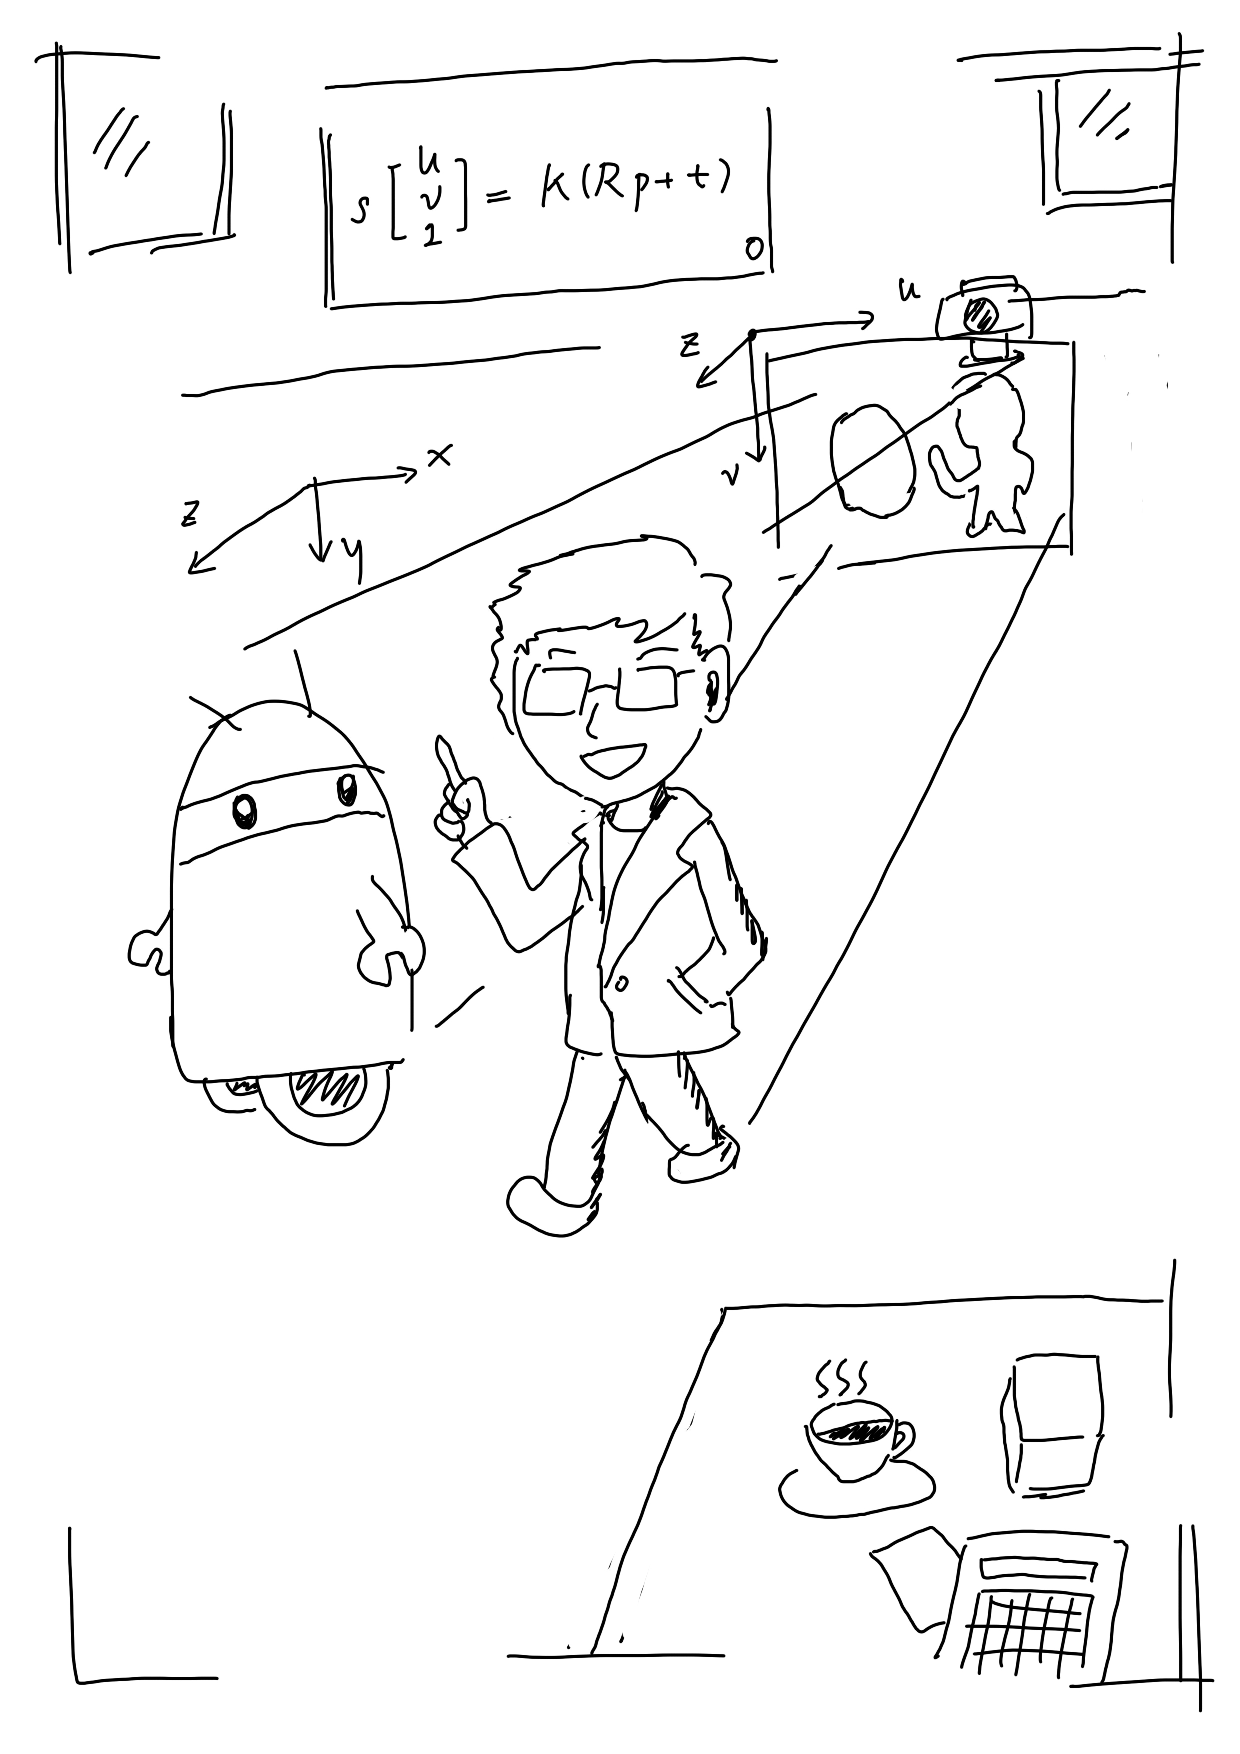
\includepdf{resources/other/ch5.pdf}
\newpage
\section{Pinhole Camera Models}
The process of projecting a 3D point (in meters) to a 2D image plane (in pixels) can be described by a geometric model. Actually, several models describe this, the simplest of which is called the pinhole model. We will start with this pinhole projection. At the same time, due to the presence of the lens on the camera lens, \textit{distortion} is generated during the projection. Therefore, we will use the pinhole model plus a distortion model to describe the entire projection process.

\subsection{Pinhole Camera Geometry}
Most of us have seen the candle projection experiment in the physics class of high school: a lit candle is placed in front of a dark box, and the light of the candle is projected through a small hole in the dark box on the rear plane. Then an inverted candle image is formed on this plane. In this process, the small hole can project a candle in a three-dimensional world onto a two-dimensional imaging plane. For the same reason, we can use this simple model to explain the camera's imaging process, as shown in \autoref{fig:cameraModel}.

\begin{figure}[!ht]
	\centering
	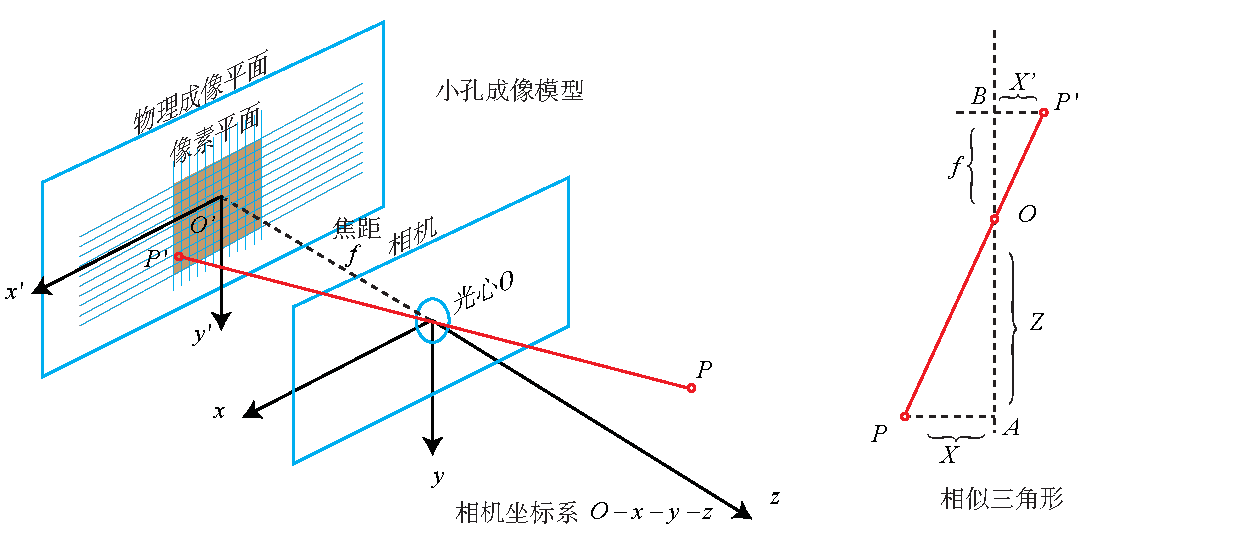
\includegraphics[width=.95\textwidth]{cameraModel/cameraModel.pdf}
	\caption{Pinhole camera model. }
	\label{fig:cameraModel}
\end{figure}

Let's take a look at the simple geometry in this model. Let $O-x-y-z$ be the camera coordinate system. Commonly we put the $z$ axis to the front of the camera, $x$ to the right, and $y$ to the down (so in this figure, we should stand on the left side to see the right side). $O$ is the camera's optical center, which is also the ``hole'' in the pinhole model. The 3D point $P$, after being projected through the hole $O$, falls on the physical imaging plane $O'-x'-y'$ and produces the image point $P'$. Let the coordinates of $P$ be $[X,Y,Z]^T$, $P'$ is $[X',Y',Z']^T$, and set the physical distance from the imaging plane to camera plane is $f$ (focal length). Then, according to the similarity of the triangles, there are:
\begin{equation}
\frac{Z}{f} = -\frac{X}{{X'}} =-\frac{Y}{{Y'}}.
\end{equation}

The negative sign indicates that the image is inverted. However, the image obtained by modern cameras is not inverted (otherwise, the usage of the camera would be very inconvenient). To make the model more realistic, we can equivalently place the imaging plane symmetrically in front of the camera, as shown by \autoref{fig:planes}. This can remove the negative sign in the formula to make it more compact:
\begin{equation}
\frac{Z}{f} = \frac{X}{{X'}} =\frac{Y}{{Y'}}.
\end{equation}

\begin{figure}[!htp]
	\centering
	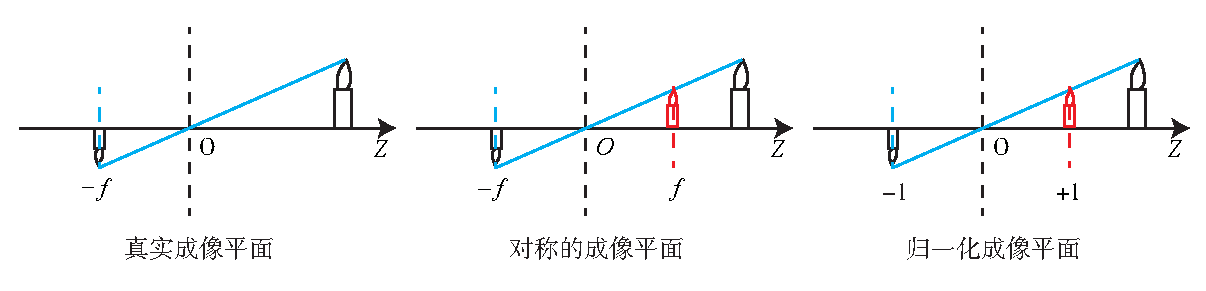
\includegraphics[width=1.0\textwidth]{cameraModel/planes.pdf}
	\caption{The real, symmetric and normalized image plane.}
	\label{fig:planes}
\end{figure}

Put $X', Y'$ to the left side:
\begin{equation}\label{eq:P2Pprime}
X' = f\frac{X}{Z}, \quad Y' = f\frac{Y}{Z}.
\end{equation}

Readers may ask why we can arbitrarily move the imaging plane to the front? In fact, this is just a mathematical approach to handle the camera projection, and most of the images captured by the camera are not upside-down. The camera's software will flip the picture for you, so what we actually get is the symmetric plane's image. Although the pin-hole image should be inverted from the physical principle since we have pre-processed the picture, it is not wrong to take the symmetric one. Therefore, without causing ambiguity, we often emit the minus symbol in the pin-hole model.


The formula~\eqref{eq:P2Pprime} describes the spatial relationship between the point $P$ and its image, where the units of all points are meters. For example, a focal length maybe 0.2 meters, and $X'$ be 0.14 meters. However, in the camera, we end up with pixels, where we need to sample and quantize the pixels on the imaging plane. To describe how the sensor converts the perceived light into image pixels, we set a pixel plane $o-u-v$ fixed on the physical imaging plane. Finally, we get \textit{pixel coordinates} of $P'$ in the pixel plane: $[u,v]^T$.

The usual definition of the pixel coordinate system \footnote{ Or image coordinate system, see section 2 of this lecture. } is: the origin $o'$ is in the upper left corner of the image, the $u$ axis is parallel to the $x$ axis, and the $v$ axis is parallel to the $y$ axis. Between the pixel coordinate system and the imaging plane, there is an apparent \textit{zoom} and a \textit{translation of the origin}. We set the pixel coordinates to scale $\alpha$ times on the $u$ axis and $\beta$ times on $v$. At the same time, the origin is translated by $[c_x, c_y]^T$. Then, the relationship between the coordinates of $P'$ and the pixel coordinate $[u,v]^T$ is:
\begin{equation}
\label{eq:project2pixel1} 
\left\{
\begin{matrix} 
u=\alpha X' + c_x\\ 
v=\beta Y' + c_y
\end{matrix}
\right. .
\end{equation}

Put it into~\eqref{eq:P2Pprime} and set $\alpha f$ as $f_x$, $\beta f$ as $f_y$:
\begin{equation}
\left\{
\begin{matrix} 
u=f_x\frac{X}{Z} + c_x\\ 
v=f_y\frac{Y}{Z} + c_y
\end{matrix}
\right. ,
\end{equation}
where $f$ is the focal length in meters, $\alpha, and \beta$ is in pixels/meter, so $f_x, f_y$ and $c_x, c_y$ are in pixels. It would be more compact to write this form as a matrix, but we need to use homogeneous coordinates on the left and non-homogeneous coordinates on the right:
\begin{equation}
\label{eq:intrinmatrix} 
\begin{pmatrix} u\\ v\\ 1 \end{pmatrix}=\frac{1}{Z}\begin{pmatrix} f_x & 0&c_x \\ 0& f_y& c_y\\ 0&0 & 1 \end{pmatrix}\begin{pmatrix} X\\ Y\\ Z \end{pmatrix} 
\buildrel \Delta \over =\frac{1}{Z} \mathbf{K} \mathbf{P}.
\end{equation}

Let's put $Z$ to the left side as in most books:
\begin{equation}
Z \begin{pmatrix} u\\ v\\ 1 \end{pmatrix}= \begin{pmatrix} f_x & 0&c_x \\ 0& f_y& c_y\\ 0&0 & 1 \end{pmatrix}\begin{pmatrix} X\\ Y\\ Z \end{pmatrix} 
\buildrel \Delta \over = \mathbf{K} \mathbf{P}.
\end{equation}

In this equation, we refer to the matrix composed of the middle quantities as the camera's inner parameter matrix (o intrinsics) $\mathbf{K}$. It is generally assumed that the camera's internal parameters are fixed after manufacturing and will not change during usage. Some camera manufacturers will tell you the intrinsics, and sometimes you need to estimate the internal parameters by yourself, which is called calibration. Because of the maturity of the calibration algorithm (such as the famous Zhang Zhengyou's calibration {\cite{Zhang1999}}), it will not be introduced here \footnote{I'm sure professor Zhang has a copy of this book now.}. 

There are internal parameters, and naturally, there must be something like ``external parameters''. In the equation ~\eqref{eq:intrinmatrix}~, we use the coordinates of $P$ in the camera coordinate system, but in fact, the coordinates of $P$ should be its world coordinates because the camera is moving (we use the symbol $\mathbf{P}_w$). It should be converted to the camera coordinate system based on the current pose of the camera. The camera's pose is described by its rotation matrix $\mathbf{R}$ and the translation vector $\mathbf{t}$. Then there are:

\begin{equation}
\label{eq:cameraprojection}
Z \mathbf{P}_{uv}=
Z \left[ \begin{array}{l}
u\\
v\\
1
\end{array} \right] = \mathbf{K} \left( {\mathbf{R}{ \mathbf{P}_w} + \mathbf{t}} \right) =  \mathbf{K} \mathbf{T} \mathbf{P}_w .
\end{equation}

Note that the latter formula implies a conversion from homogeneous to non-homogeneous coordinates (can you see it?) We use homogeneous coordinates in $\mathbf{T}\mathbf{P}$, then convert to non-homogeneous coordinates, and then multiply it by $\mathbf{K}$.  It describes the projection relationship of world coordinates to pixel coordinates of $P$. Among them, the camera's pose $\mathbf{R}, \mathbf{t}$ is also called the camera's \textit{extrinsics}. \footnote{In robots or autonomous vehicles, extrinsics is often defined as the transform between the camera coordinate system and the robot body coordinate system, describing ``where the camera is installed''.}  Compared with the intrinsic, the extrinsics may change with the camera installation and is also the target to be estimated in the SLAM if we only have a camera.

The projection process can also be viewed from another perspective. The formula ~\eqref{eq:cameraprojection} shows that we can convert a world coordinate point to the camera coordinate system first and then remove the last dimension. The depth of the point from the imaging plane of the camera is then removed, which is equivalent to the normalization on the last dimension. In this way, we get the projection of the point $P$ on the camera \textit{normalized plane}:
\begin{equation}
\left( {\mathbf{R}{\mathbf{P}_w} + \mathbf{t}} \right) = \underbrace{\left[ X,Y,Z\right]^T}_{\text{Camera Coordinates}} \to \underbrace {\left[ {X/Z,Y/Z,1} \right]^T}_{\text{Normalized Coordinates}}.
\end{equation}

The \textit{normalized coordinates} can be seen as a point in the $z=1$ plane in front of the camera \footnote{Note that in the calculation, it is necessary to check whether $Z$ is positive because the negative $Z$ can also get the point on the normalized plane by this method. However, the camera does not capture the scene behind the imaging plane. }.This $z=1$ plane is also called \textit{normalized plane}. We normalize the coordinates and then multiply them with the intrinsic matrix, yielding the pixel coordinates. We can also consider the pixel coordinates $[u,v]^T$ as the result of quantitative measurements on points on the normalized plane. If the camera coordinates are multiplied by any non-zero constant simultaneously, the normalized coordinates are the same, which means that the depth is lost during the projection process. So, in monocular vision, the pixel's depth value cannot be obtained by a single image.

\subsection{Distortion}
In order to get a larger FoV (Field-of-View), we usually add a lens in front of the camera. The addition of the lens has an influence on the propagation of light during imaging: (1) the shape of the lens may affect the propagation way of light, (2) during the mechanical assembly, the lens and the imaging plane are not entirely parallel, which also changes the projected position.

There are some mathematical models to describe the distortion caused by the shape of the lens. In the pinhole model, a straight line keeps straight when projected onto the pixel plane. However, in real photos, the camera lens tends to make a straight line in the real environment become a curve \footnote{Yes, it is no longer straight but becomes curved. If it makes an inside curve, it is called barrel-like distortion; otherwise, it is cushion-like distortion if the curve looks outward. }. The closer to the edge of the image, the more obvious this phenomenon is. Since the lenses actually produced are often center-symmetrical, this makes the irregular distortion generally radially symmetrical. They fall into two main categories: \textit{barrel-like distortion} and \textit{cushion-like distortion}, as shown by \autoref{fig:distortion}.
\begin{figure}[!t]
	\centering
	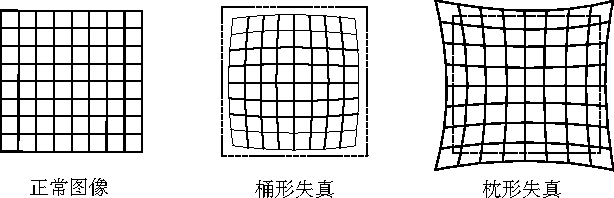
\includegraphics[width=0.7\textwidth]{cameraModel/distortion.pdf}
	\caption{The radical distortion.}
	\label{fig:distortion}
\end{figure}

In barrel distortion, the radius of pixels decreases as the optical axis's distance increases, while the cushion distortion is just the opposite. In both distortions, the line that intersects the center of the image and the optical axis remains the same.

In addition to the shape of the lens, which introduces radial distortion, \textit{tangential distortion} is introduced during assembly of the camera because the lens and the imaging surface cannot be strictly parallel, as shown by \autoref{fig:tangen}.

\begin{figure}[!t]
	\centering
	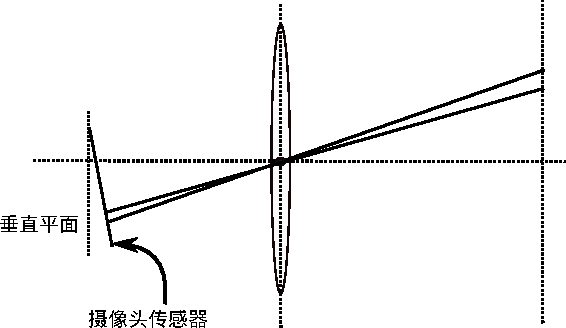
\includegraphics[width=0.7\textwidth]{cameraModel/tangen.pdf}
	\caption{Tangential distortion.}
	\label{fig:tangen}
\end{figure}
To better understand radial and tangential distortion, we describe them in a more rigorous mathematical form. Consider any point on the \textit{normalized plane}, $\mathbf{p}$, whose coordinates are $[x,y]^T$, or $[r, \theta]^T$ in the form of polar coordinates, where $r$ represents the distance between the point $\mathbf{p}$ and the origin of the coordinate system, and $\theta$ represents the angle to the horizontal axis. Radial distortion can be seen as a change in the coordinate point along the length, that is, its radius from the origin. Tangential distortion can be seen as a change in the coordinate point along the tangential direction, which means that the horizontal angle has changed. It is generally assumed that these distortions are polynomial, namely:
\begin{equation}
\label{eq:distortion} 
\begin{matrix}
x_\mathrm{distorted} = x(1+k_1r^2+k_2r^4+k_3r^6)\\
y_\mathrm{distorted} = y(1+k_1r^2+k_2r^4+k_3r^6)
\end{matrix},
\end{equation}
where $[x_\mathrm{distorted}, y_\mathrm{distorted}]^T$ is the \textit{normalized coordinates} of the point after distortion. On the other hand, for \textit{tangential distortion}, we can use the other two parameters $p_1,p_2$ to describe it:
\begin{equation}
\label{eq:tangen} 
\begin{matrix}
x_\mathrm{distorted} = x+2p_1xy+p_2(r^2+2x^2)\\
y_\mathrm{distorted} = y+p_1(r^2+2y^2)+2p_2xy
\end{matrix}. 
\end{equation}
Putting~\eqref{eq:distortion} and~\eqref{eq:tangen} together we get a joint model with 5 distortion coefficients. The complete form is:
\begin{equation}
\left\{\begin{matrix} x_\mathrm{distorted} =x(1+k_1r^2+k_2r^4+k_3r^6)+2p_1xy+p_2(r^2+2x^2)\\ 
y_\mathrm{distorted} = y(1+k_1r^2+k_2r^4+k_3r^6)+p_1(r^2+2y^2)+2p_2xy
\end{matrix}\right. .
\end{equation}

In the above process of correcting distortion, we used 5 distortion coefficients. In practical applications, you can flexibly choose to number of parameters, for example, only selecting $k_1, p_1, p_2$, or use $k_1, k_2, p_1, p_2$, etc.

This section models the camera's imaging process using a pinhole model and described the radial and tangential distortions caused by the lens. Researchers have proposed many other models in the existing imaging system, such as the affine model and perspective model, and there are many different types of distortion. In most visual SLAM systems, pinhole and rad-tan distortion models are sufficient, so we will not describe the other ones.

It is worth mentioning that there are two ways of undistortion (or correction). We can choose to undistort the entire image first, get the corrected image, and then discuss the spatial position of the points on the image. Alternatively, we can also extract some feature points in the distorted image and find its real position through the distortion equation. Both are feasible, but the former seems to be more common in visual SLAM. Therefore, when an image is undistorted, we can directly establish a projection relationship with the pinhole model without considering distortion. Therefore, in the discussion that follows, we can directly assume that the image has been undistorted.

Finally, let's summarize the imaging process of a monocular camera:

\begin{enumerate}
	\item First, there is a point $P$ in the world coordinate system, and its world coordinates are $\mathbf{P}_w$.
	\item Since the camera is moving, its motion is described by $\mathbf{R}, \mathbf{t}$ or  transform matrix $\mathbf{T} \in \mathrm{SE}(3)$. The camera coordinates for $P$ are $\tilde{\mathbf{P}}_c = \mathbf{R} \mathbf{P}_w + \mathbf{t}$.
	\item The $\tilde{\mathbf{P}}_c$ components are $X,Y, Z$, and they are projected onto the normalized plane $Z=1$ to get the normalized coordinates: $\mathbf{P}_c = [X/Z, Y/Z, 1]^T$. Note that $Z$ may be less than 1, indicating that the point is behind the normalization plane and it should not be projected on the camera plane.
	\item If the image is distorted, the coordinates of $\mathbf{P}_c$ after distortion are calculated according to the distortion parameters.
	\item Finally, the distorted coordinates of $P$ pass through the intrinsics and we find its pixel coordinates: $\mathbf{P}_{uv} = \mathbf{K} \mathbf{P}_c$.
\end{enumerate}

In summary, we have talked about four coordinates: the world coordinates, the camera coordinates, the normalized coordinates, and the pixel coordinates. Readers should clarify their relationship. They reflect the entire imaging process and will be used in the future.

\subsection{Stereo Cameras}
The pinhole camera model describes the imaging model of a single camera. However, we cannot determine the specific location of a spatial point only by a single pixel. This is because all points on the line from the camera's optical center to the normalized plane can be projected onto that pixel. Only when the depth of $P$ is determined (such as through a binocular or RGB-D camera) can we know exactly its spatial location, as shown in \autoref {fig:pixelLocation}~.

\begin{figure}[!ht]
    \centering
    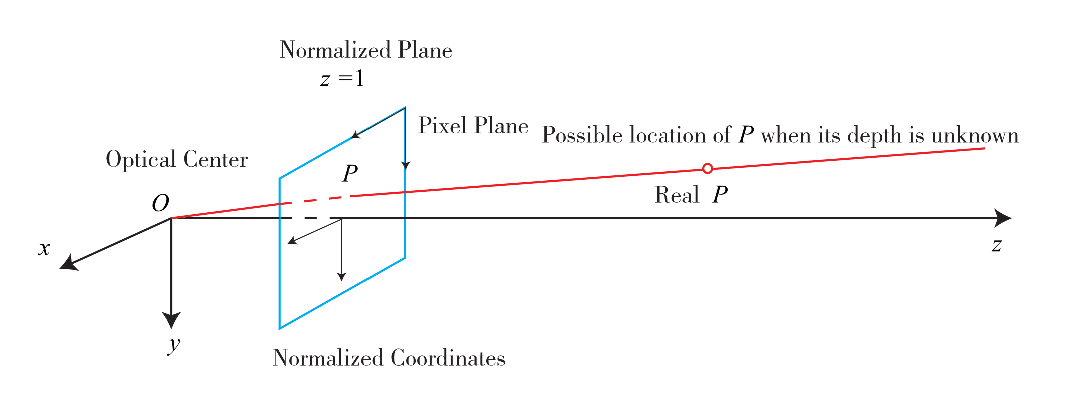
\includegraphics[width=1.0\textwidth]{cameraModel/pixelLocation.pdf}
    \caption{The possible location of a single pixel.}
    \label{fig:pixelLocation}
\end{figure}

There are many ways to measure the pixel distance (or depth). For example, the human eye can judge the object's distance according to the difference (or parallax) of the scene seen by the left and right eyes. The binocular camera principle is also the same. By simultaneously acquiring the left and right cameras' images and calculating the parallax/disparity between the images, each pixel's depth is estimated. In the following paragraph, we briefly describe the stereo camera's imaging principle (as shown in \autoref{fig:stereoCamera}~).

A binocular camera is generally composed of a left-eye camera and a right-eye camera. Of course, it can also be made up and down, but the mainstream binoculars we've seen are all left and right. Both the left and right cameras are regarded as simple pinhole cameras. They are synchronized and placed horizontally, meaning that both cameras' centers are on the same $x$ axis. The distance between the two centers is called \textit {baseline} (denoted as $b$), which is an important parameter.

\begin{figure}[!ht]
    \centering
    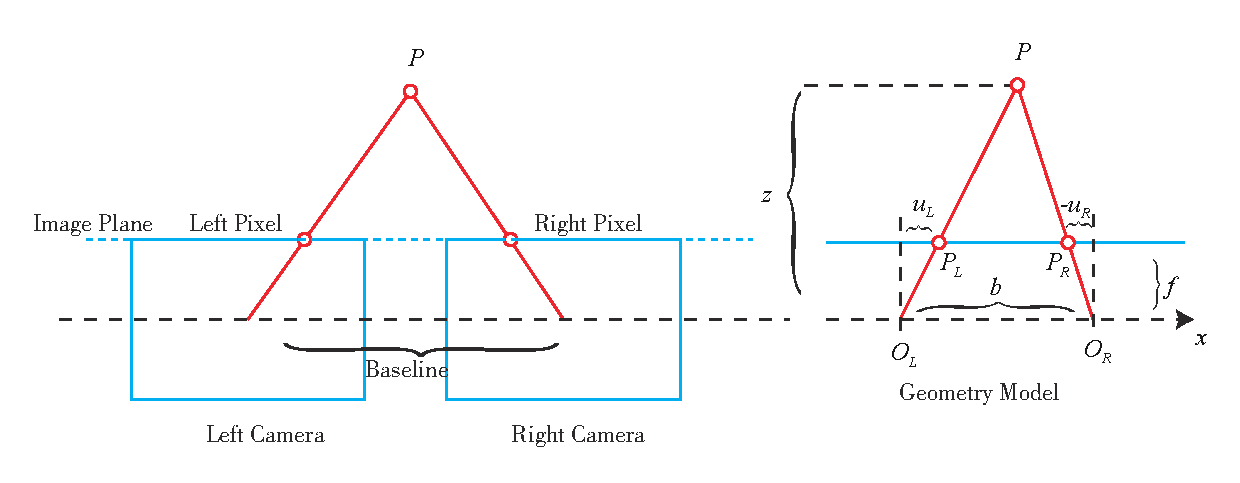
\includegraphics[width=1.0\textwidth]{cameraModel/stereoCamera.pdf}
    \caption{Geometry model of stereo cameras from upside down view. The $O_L, O_R$ are left and right optical centers. $f$ is the focal length, $u_L$ and $u_R$ are pixel coordinates of the same point along the $x$ axis. Note that $u_R$ should be a negative value in this figure, so the physical distance should be $-u_R$.}
    \label{fig:stereoCamera}
\end{figure}

Now consider a 3D point $P$, projected into the left-eye and the right-eye, written as $P_L, P_R$. Due to the presence of the camera baseline, these two imaging positions are different. Ideally, since the left and right cameras are only shifted on the $x$ axis, the image of $P$ also differs only on the $x$ axis (corresponding to the $u$ axis of the image). Take the left pixel coordinate as $u_L$ and the right coordinate as $u_R$. The geometric relationship is shown on the right of \autoref{fig:stereoCamera}. According to the similarity relationship between $ \triangle P P_L P_R$ and $\triangle P O_L O_R$, there are:

\begin{equation}
\frac{{z - f}}{z} = \frac{{b - {u_L} + {u_R}}}{b}.
\end{equation}

Rearrange it, and we have:
\begin{equation}
z = \frac{{fb}}{d}, \quad d \buildrel \Delta \over = {u_L} - {u_R},
\end{equation}
where $d$ is defined as the difference between the left and right figures' horizontal coordinates and is called disparity or parallax. Based on the parallax, we can estimate the distance between a pixel and the camera. Parallax is inversely proportional to distance: the larger the parallax is, the closer the distance is \footnote {Readers can simulate it with your own eyes.}. Simultaneously, since the parallax is at least one pixel, there is a theoretical maximum value for the binocular depth, which is determined by $fb$. To see the far-away things, we need a larger stereo camera; conversely, small binocular devices can only measure very close distances. By analogy, when the human eye looks at a very distant object (such as a very distant airplane), it is usually impossible to determine its distance accurately.

Although the depth's formula is simple, the real calculation of $d$ itself is more complicated. We need to know precisely where a pixel of the left-eye image appears in the right-eye image (that is, the corresponding relationship). This also belongs to the kind of task that is ``easy for humans but difficult for computers''. When we want to calculate each pixel's depth in an image, the calculation amount and accuracy will become a problem, and the parallax can be calculated only in the place where the image texture is rich. Due to the calculation amount, binocular depth estimation still needs GPU or FPGA to make the distance calculation run in real-time. This will be mentioned in lecture~\ref{cpt:12}.

\subsection{RGB-D Cameras}
Compared to the binocular camera's way of calculating depth, the RGB-D camera's approach is more ``active'': it can actively measure each pixel's depth. The current RGB-D cameras can be divided into two categories according to their principle (see \autoref {fig:RGBDCamera} ~):

\begin{enumerate}
\item The first kind of RGB-D sensor uses structured infrared light to measure pixel distance. Many of the old RGB-D sensors are belong to this kind, for example, the Kinect 1st generation, Project Tango 1st generation, Intel RealSense, etc.
\item The second kind measures pixel distance using the \textit{time-of-flight (ToF)}. Examples are Kinect 2 and some existing ToF sensors in cellphones.
\end{enumerate}

\begin{figure}[!ht]
    \centering
    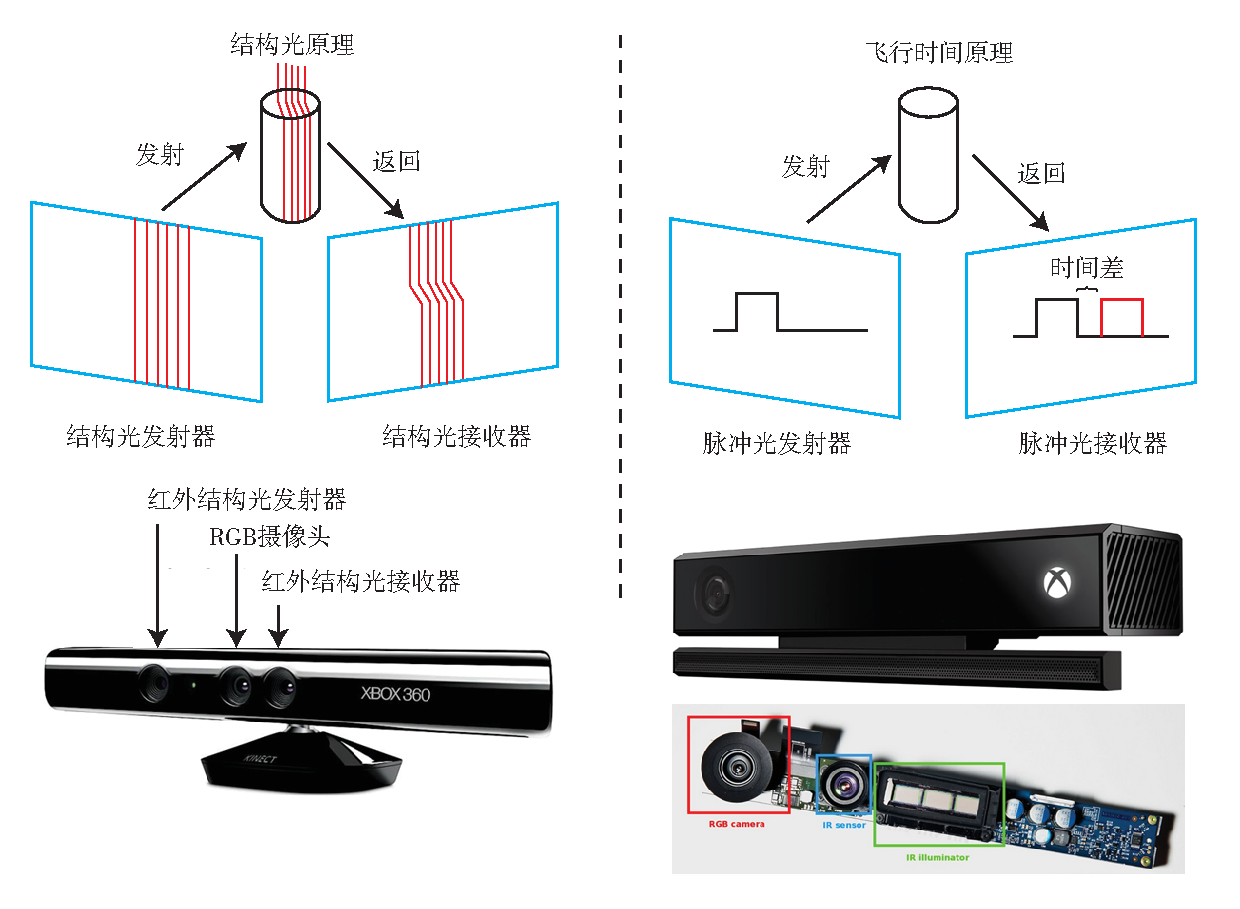
\includegraphics[width=1.0\textwidth]{cameraModel/rgbdCamera.pdf}
    \caption{RGB-D Cameras}
    \label{fig:RGBDCamera}
\end{figure}

Regardless of the type, the RGB-D camera needs to emit a light beam (usually infrared light) to the target object. In the structured light principle, the camera calculates the distance between the object and itself based on the returned structured light pattern. In the ToF principle, the camera emits a light pulse to the target and then determines the distance according to the beam's time of flight. The ToF principle is very similar to the laser sensor, except that the laser obtains the distance by scanning point by point (or line by line). The ToF camera can obtain the entire image's pixel depth, which is also the RGB-D camera's main advantage. So, if you take apart an RGB-D camera, you will usually find that there will be at least one transmitter and one receiver in addition to the ordinary camera.

After measuring the depth, the RGB-D camera usually completes the pairing between the depth and color map pixels according to each camera's position at the time of production. It outputs a pixel-to-pixel corresponding color image and depth image. We can read the color information and distance information at the same image position, calculate the 3D camera coordinates of the pixels, and generate a point cloud. RGB-D data can be processed either at the image level or the point cloud level. The second experiment of this lecture will demonstrate the point cloud construction of RGB-D cameras.

The RGB-D camera can measure the distance of each pixel in real-time. However, due to this measurement of transmitting and receiving, its range of use is limited. RGB-D cameras that use infrared light for depth measurement are susceptible to interference from infrared light emitted by daylight or other sensors, so they cannot be used outdoors. Without modulation, multiple RGB-D cameras can interfere with each other. These points' positions cannot be measured for transparent objects because they cannot receive reflected light. Also, RGB-D cameras have some disadvantages in terms of cost and power consumption.

\section{Images}
Cameras and lens convert the information in the three-dimensional world into a photo composed of pixels, which is then stored in the computer as a data source for subsequent processing. In mathematics, images can be described by a matrix; in computers, they occupy a continuous disk or memory space, which can be represented by a two-dimensional array. In this way, the program does not have to distinguish whether they are dealing with a numerical matrix or a meaningful image.

In this section, we will introduce some basic operations of computer image processing. In particular, we are going to introduce the basic steps of processing images with OpenCV and lay the foundation for subsequent chapters. Let's start with the simplest case, the grayscale image. Each pixel position $ (x, y) $ corresponds to a grayscale value of $ I $ in a grayscale image. Therefore, an image with the width of $ w $ and the height of $ h $ can be mathematically written as a function:
\[
(I) (x, y): \mathbb {R} ^ 2 \mapsto \mathbb {R},
\]
where $ (x, y) $ is the coordinate of the pixel. However, computers cannot express real numbers, so we need to quantify the subscripts and image readings within a certain range. For example, $ x, y $ are usually integers starting with 0 to $w-1, h-1$. In common grayscale images, an integer of $0 \textasciitilde 255$ (that is, an unsigned char in C++, 1 byte) is used to express the grayscale reading of the image. Then, a grayscale image with a width of 640 pixels and a height of 480 pixels can be expressed as:
\begin{lstlisting}[language=C++, caption=Use 2D array to express an image]
unsigned char image[480][640];
\end{lstlisting}

Why does the two-dimensional array here have the size of 480 $ \times $ 640? Because in the program, the first index of the 2D array is the row, and the second index is the column. In an image, the number of rows (or the $y$ axis) in the array corresponds to the height of the image, and the number of columns (or the $x$ axis) corresponds to the width of the image.
\begin{figure}[!t]
    \centering
    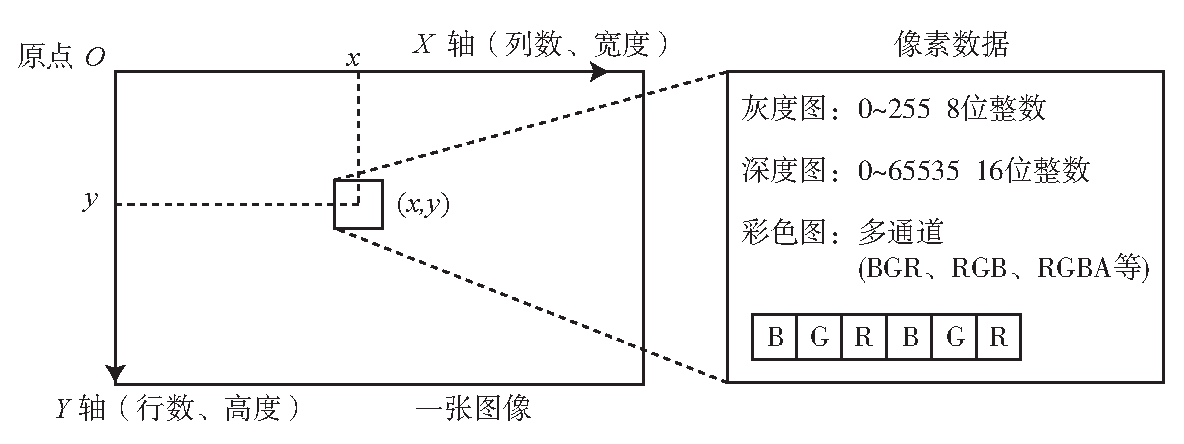
\includegraphics[width=0.84\textwidth]{cameraModel/image.pdf}
    \caption{Pixels in an image.}
    \label{fig:imagesInComputer}
\end{figure}

Let's examine the content of this image. Images are naturally made up of pixels. When accessing a certain pixel, you need to specify its coordinates, as shown in \autoref{fig:imagesInComputer}~. The left side of the figure shows how the traditional pixel coordinate system is defined. The origin is in the upper left corner of the image, the $X$ axis is from left to right, and the $Y$ is top-down. If it has a third axis, the $ Z $ axis, then according to the right-hand rule, the $ Z $ axis should be from outside to inside (or front in 3D space). This definition is consistent with the camera coordinate system. The width or number of columns of an image corresponds to the $ X $ axis; the number of rows or the height of an image corresponds to its $ Y $ axis.

According to this definition, if we discuss a pixel located at $x,y$, then the code of accessing its memory in the computer should be:
\begin{lstlisting}[language = C++, caption = Accessing image pixels]
unsigned char pixel = image[y][x];
\end{lstlisting}

It corresponds to the reading of the gray value $ I(x,y) $. Please note the order of $ x $ and $ y $ here. Although we tirelessly discuss the problem of coordinate systems, errors like this index sequence will still be one of the most common errors encountered by novices during debugging. If you accidentally change the coordinates of $ x, y $ when writing a program, the compiler cannot provide any useful information at compile-time. All you can see is a segment fault in runtime.

A pixel's grayscale can be recorded as an 8-bit unsigned integer, which is a value of $0\textasciitilde 255$. If we have more information to record, one byte is probably not enough. For example, in the depth map of an RGB-D camera, each pixel's distance is recorded. This distance is usually measured in millimeters, and the range of RGB-D cameras is usually around a dozen meters, exceeding 255. At this time, people will use 16-bit integers (unsigned short in C++) to record the depth map information, that is, the value at $0 \textasciitilde 65535$. When converted to meters, it can represent up to 65 meters, which is enough for RGB-D cameras.

The representation of a color image requires the concept of a channel. In computers, we use three colors: red, green, and blue to express any color. Therefore, for each pixel, three R, G, and B values are recorded, and each value is called a channel. For example, the most common color image has three channels, represented by an 8-bit integer. Under this rule, one pixel occupies a 24-bit space.

The number and order of channels can be freely defined. In OpenCV color images, the default order of channels is B, G, R, which means when we get a 24-bit pixel, the first 8 bits represent the blue value, the middle 8 bits represent the green, and the last 8 bits represent the red. Similarly, the order of R, G, and B can also be used to describe a color image. If you want to express the image's transparency, use R, G, B, A four channels.

\section{Practice: Images in Computer Vision}
\subsection{Basic Usage of OpenCV}
The following is a demo program to help you understand how to access the image in OpenCV and how to visit its pixels.

\subsubsection{Install OpenCV}
OpenCV \footnote {Official homepage: \url{http://opencv.org}. } provides many open-source image algorithms and is a very widely used image processing algorithm library in computer vision. This book also uses OpenCV for basic image processing. Before using, readers must install it from the pre-compiled library or from source code. Under Ubuntu, there are two options: \textit{install from source code} or \textit {only install binary library files}:

\begin{enumerate}
\item Install from source means to download all OpenCV source code from the OpenCV website, compile and install on the machine for usage. The advantage is that you can freely choose which version to install, and the source code is accessible, but it takes some compilation time.
\item Or, we can only install the binary library file, which means it was pre-compiled by the Ubuntu community, so there is no need to recompile it.
\end{enumerate}

If we use a newer version of OpenCV than that in the apt source, we must install it from the source code. First, you can adjust some compilation options to match the programming environment (for example, to disable some unused modules or turn on the GPU acceleration, etc.). OpenCV currently maintains two major versions, divided into OpenCV 2.4 series and OpenCV 3 series \footnote{In 2020, we can also use version 4.0 or higher.}. This book uses the OpenCV \textit {3} or higher.

Because the OpenCV project is relatively large, it will not be placed under 3rdparty in this book. Readers can download it from ~ \url{http://opencv.org/downloads.html}~ and select the Linux version. You will get a compressed package like opencv-3.1.0.zip. Unzip it to any directory, we can found that OpenCV is also a CMake project.

Before compiling, first, install the dependencies of OpenCV:
\begin{lstlisting}[language=sh, caption=Terminal input:]
sudo apt-get install build-essential libgtk2.0-dev libvtk5-dev libjpeg-dev libtiff4-dev libjasper-dev libopenexr-dev libtbb-dev
\end{lstlisting}

In fact, OpenCV has many dependencies, and the lack of certain dependency items will affect some of its functions (but we will not use all the functions). OpenCV will check whether the dependencies will be installed during CMake and adjust its own configurations. If you have a GPU on your computer and the relevant dependencies are installed, OpenCV will also enable GPU acceleration. But for this book, the above dependencies are sufficient.

Subsequent compilation and installation are the same as ordinary CMake projects. After make, please call ``sudo make install'' to install OpenCV on your machine (instead of just compiling it). Depending on the machine configuration, this compilation process may take from 20 minutes to an hour. If your CPU is powerful, you can use commands like ``make -j4'' to call multiple threads to compile (the parameter after -j is the number of threads used). After installation, OpenCV is stored in the /usr/local directory by default. You can look for OpenCV header files and library files' installation location to see where they are. Besides, if you have installed the OpenCV 2 series before, it is recommended that you install OpenCV 3 elsewhere (think about how this should be done).

\subsection{Basic OpenCV Images Operations}
Now let's go through the basic image operations in OpenCV from a simple example.

\begin{lstlisting}[language=C++,caption=slambook/ch5/imageBasics/imageBasics.cpp]
#include <iostream>
#include <chrono>

using namespace std;

#include <opencv2/core/core.hpp>
#include <opencv2/highgui/highgui.hpp>

int main(int argc, char **argv) {
    // Read the image in argv[1]
    cv::Mat image;
    image = cv::imread(argv[1]); // call cv::imread to read the image from file
    
    // check the data is correctly loaded
    if (image.data == nullptr) { // maybe the file does not exist
        cerr << "file" << argv[1] << " not exist." << endl;
        return 0;
    }
    
    // print some basic information
    cout << "Image cols: " << image.cols << ", rows: " << image.rows 
	    << ", channels: " << image.channels() << endl;
    cv::imshow("image", image);      // use cv::imshow to show the image
    cv::waitKey(0);                  // display and wait for a keyboard input
    
    // check image type
    if (image.type() != CV_8UC1 && image.type() != CV_8UC3) {
        // we need grayscale image or RGB image
        cout << "image type incorrect." << endl;
        return 0;
    }
    
    // check hte pixels
    chrono::steady_clock::time_point t1 = chrono::steady_clock::now();
    for (size_t y = 0; y < image.rows; y++) {
        // use cv::Mat::ptr to get the pointer of each row
        unsigned char *row_ptr = image.ptr<unsigned char>(y);  // row_ptr is the pointer to y-th row
        for (size_t x = 0; x < image.cols; x++) {
            // read the pixel on (x,y), x=column, y=row
            unsigned char *data_ptr = &row_ptr[x * image.channels()]; // data_ptr is the pointer to (x,y)
            // visit the pixel in each channel
            for (int c = 0; c != image.channels(); c++) {
                unsigned char data = data_ptr[c]; // data should be pixel of I(x,y) in c-th channel
            }
        }
    }
    chrono::steady_clock::time_point t2 = chrono::steady_clock::now();
    chrono::duration<double> time_used = chrono::duration_cast < chrono::duration < double >> (t2 - t1);
    cout << "time used: " << time_used.count() << " seconds." << endl;
    
    // copying cv::Mat
    // operator = will not copy the image data, but only the reference
    cv::Mat image_another = image;
    // changing image_another will also change image 
    image_another(cv::Rect(0, 0, 100, 100)).setTo(0); // set top-left 100*100 block to zero
    cv::imshow("image", image);
    cv::waitKey(0);
    
    // use cv::Mat::clone to actually clone the data
    cv::Mat image_clone = image.clone();
    image_clone(cv::Rect(0, 0, 100, 100)).setTo(255);
    cv::imshow("image", image);
    cv::imshow("image_clone", image_clone);
    cv::waitKey(0);
    
    // We are not going to copy the OpenCV's documentation here
    // please take a look at it for other image operations like clipping, rotating and scaling.
    
    cv::destroyAllWindows();
    return 0;
}
\end{lstlisting}

In this example, we demonstrated the following operations: image reading, displaying, pixel vising, copying, assignment, etc. When compiling the program, you need to add the OpenCV header file in your ``CMakeLists.txt'', and then link the program to the OpenCV's library. At the same time, due to the use of C++ 11 standards (such as the nullptr and chrono), you also need to set up the c++ standard in the compiler flag:

\begin{lstlisting}[language=Python,caption=slambook/ch5/imageBasics/CMakeLists.txt]
# use c++11 standard
set( CMAKE_CXX_FLAGS "-std=c++11" )

# find OpenCV
find_package( OpenCV REQUIRED )
# include its headers
include_directories( ${OpenCV_INCLUDE_DIRS} )

add_executable( imageBasics imageBasics.cpp )

# link the exe to opencv's libs
target_link_libraries( imageBasics ${OpenCV_LIBS} )
\end{lstlisting}

Let's give some notes for the code:
\begin{enumerate}
\item The program reads the image position from argv[1], the first parameter on the command line. We prepared an image (ubuntu.png, an Ubuntu wallpaper, hope you like it) for readers to test. Therefore, after compilation, use the following command to call this program:
\begin{lstlisting}[language=sh, caption=Terminal input:]
./build/imageBasics ubuntu.png
\end{lstlisting}
If you call this program in the IDE, be sure to give it parameters at the same time. This can be configured in the launch configuration dialog if you are using Clion.
\item In line 10 \textasciitilde to 18, we use the cv::imread function to read the image. And then, we display the image and its basic information.
\item In line 35 \textasciitilde 46, we iterate over all pixels in the image and calculates the time spent in the entire loop. Please note that the pixel visiting method is not unique, and the method given by the example is not the most efficient way. OpenCV provides an iterator of cv::Mat. You can traverse the pixels of the image through the iterator. Or, cv::Mat::data provides a raw pointer to the beginning of the image data. You can also directly calculate the offset through this pointer, and then get the memory location of the pixel. The method used in the example is to facilitate the reader to understand the structure of the image.

\item OpenCV provides many functions for manipulating images. We will not list them one by one. Otherwise, this book will become an OpenCV operation manual. The example shows the most common things like image reading and displaying and the deep copy function in cv::Mat. During the programming process, readers will also encounter operations such as image rotation and interpolation. At this time, you should refer to the corresponding documentation of the function to understand their principles and usage.
\end{enumerate}

It should be noted that OpenCV is not the only image library. It is just one of the more widely used ones. However, most image libraries have similar image operations. We hope that readers can understand the representation of images in other libraries after using OpenCV to quickly adjust to any other libraries. Since cv::Mat is also a matrix class, we can also use it to store matrix data such as rotation matrix and do some linear algebra operations. But it is generally believed that \textit{Eigen} is more efficient for use with fixed-size matrices.

\subsection{Image Undistortion}
We've introduced the rad-tan distortion model in the previous section, now let write an example to show the implementation. OpenCV has provided the cv::Undistort function for us, but we will also give a hand-written undistortion function to show the principles.

\begin{lstlisting}[language=C++,caption=slambook/ch5/imageBasics/undistortImage.cpp]
#include <opencv2/opencv.hpp>
#include <string>
using namespace std;
string image_file = "./distorted.png";   // the distorted image 

int main(int argc, char **argv) {
    // In thie program we implement the undistortion by ourselves rather than using opencv
    // rad-tan model params
    double k1 = -0.28340811, k2 = 0.07395907, p1 = 0.00019359, p2 = 1.76187114e-05;
    // intrinsics
    double fx = 458.654, fy = 457.296, cx = 367.215, cy = 248.375;
    
    cv::Mat image = cv::imread(image_file, 0);   // the image type is CV_8UC1
    int rows = image.rows, cols = image.cols;
    cv::Mat image_undistort = cv::Mat(rows, cols, CV_8UC1);   // the undistorted image
    
    // computate the pixels in the undistorted one
    for (int v = 0; v < rows; v++) {
        for (int u = 0; u < cols; u++) {
            // note we are computing the pixel of (u,v) in the undistorted image
            // according to the rad-tan model, compute the coordinates in the distorted image
            double x = (u - cx) / fx, y = (v - cy) / fy;
            double r = sqrt(x * x + y * y);
            double x_distorted = x * (1 + k1 * r * r + k2 * r * r * r * r) + 2 * p1 * x * y + p2 * (r * r + 2 * x * x);
            double y_distorted = y * (1 + k1 * r * r + k2 * r * r * r * r) + p1 * (r * r + 2 * y * y) + 2 * p2 * x * y;
            double u_distorted = fx * x_distorted + cx;
            double v_distorted = fy * y_distorted + cy;
            
            // check if the pixel is in the image boarder
            if (u_distorted >= 0 && v_distorted >= 0 && u_distorted < cols && v_distorted < rows) {
                image_undistort.at<uchar>(v, u) = image.at<uchar>((int) v_distorted, (int) u_distorted);
            } else {
                image_undistort.at<uchar>(v, u) = 0;
            }
        }
    }
    
    // show the undistorted image
    cv::imshow("distorted", image);
    cv::imshow("undistorted", image_undistort);
    cv::waitKey();
    return 0;
}
\end{lstlisting}

Please check the difference between the two images by yourself.

\section{Practice: 3D Vision}
\subsection{Stereo Vision}
We have introduced the imaging principle of stereo vision. Now we start from the left and right images, calculate the disparity map corresponding to the left eye, and then calculate each pixel's coordinates in the camera coordinate system, which will form a \textit{point cloud}. We have prepared left and right images for the readers, as shown in \autoref {fig:stereoExample}. The following code demonstrates the calculation of disparity map and point cloud:

\begin{lstlisting}[language=C++,caption=slambook/ch5/stereoVision/stereoVision.cpp (Part)]
int main(int argc, char **argv) {
    // intrinsics
    double fx = 718.856, fy = 718.856, cx = 607.1928, cy = 185.2157;
    // baseline
    double b = 0.573;
    
    cv::Mat left = cv::imread(left_file, 0);
    cv::Mat right = cv::imread(right_file, 0);
    cv::Ptr<cv::StereoSGBM> sgbm = cv::StereoSGBM::create(
        0, 96, 9, 8 * 9 * 9, 32 * 9 * 9, 1, 63, 10, 100, 32);    // SGBM is senstive to parameters
    cv::Mat disparity_sgbm, disparity;
    sgbm->compute(left, right, disparity_sgbm);
    disparity_sgbm.convertTo(disparity, CV_32F, 1.0 / 16.0f);
    
    // compute the point cloud
    vector<Vector4d, Eigen::aligned_allocator<Vector4d>> pointcloud;
    
    // change v++ and u++ to v+=2, u+=2 if your machine is slow to get a sparser cloud
    for (int v = 0; v < left.rows; v++)
    for (int u = 0; u < left.cols; u++) {
        if (disparity.at<float>(v, u) <= 10.0 || disparity.at<float>(v, u) >= 96.0) continue;
        
        Vector4d point(0, 0, 0, left.at<uchar>(v, u) / 255.0); // the first three dimensions are xyz, the 4-th is the color
        
        // compute the depth from disparity
        double x = (u - cx) / fx;
        double y = (v - cy) / fy;
        double depth = fx * b / (disparity.at<float>(v, u));
        point[0] = x * depth;
        point[1] = y * depth;
        point[2] = depth;
        
        pointcloud.push_back(point);
    }
    
    cv::imshow("disparity", disparity / 96.0);
    cv::waitKey(0);
    
    // show the point cloud in pangolin
    showPointCloud(pointcloud);
    return 0;
}
\end{lstlisting}

\begin{figure}[!t]
    \centering
    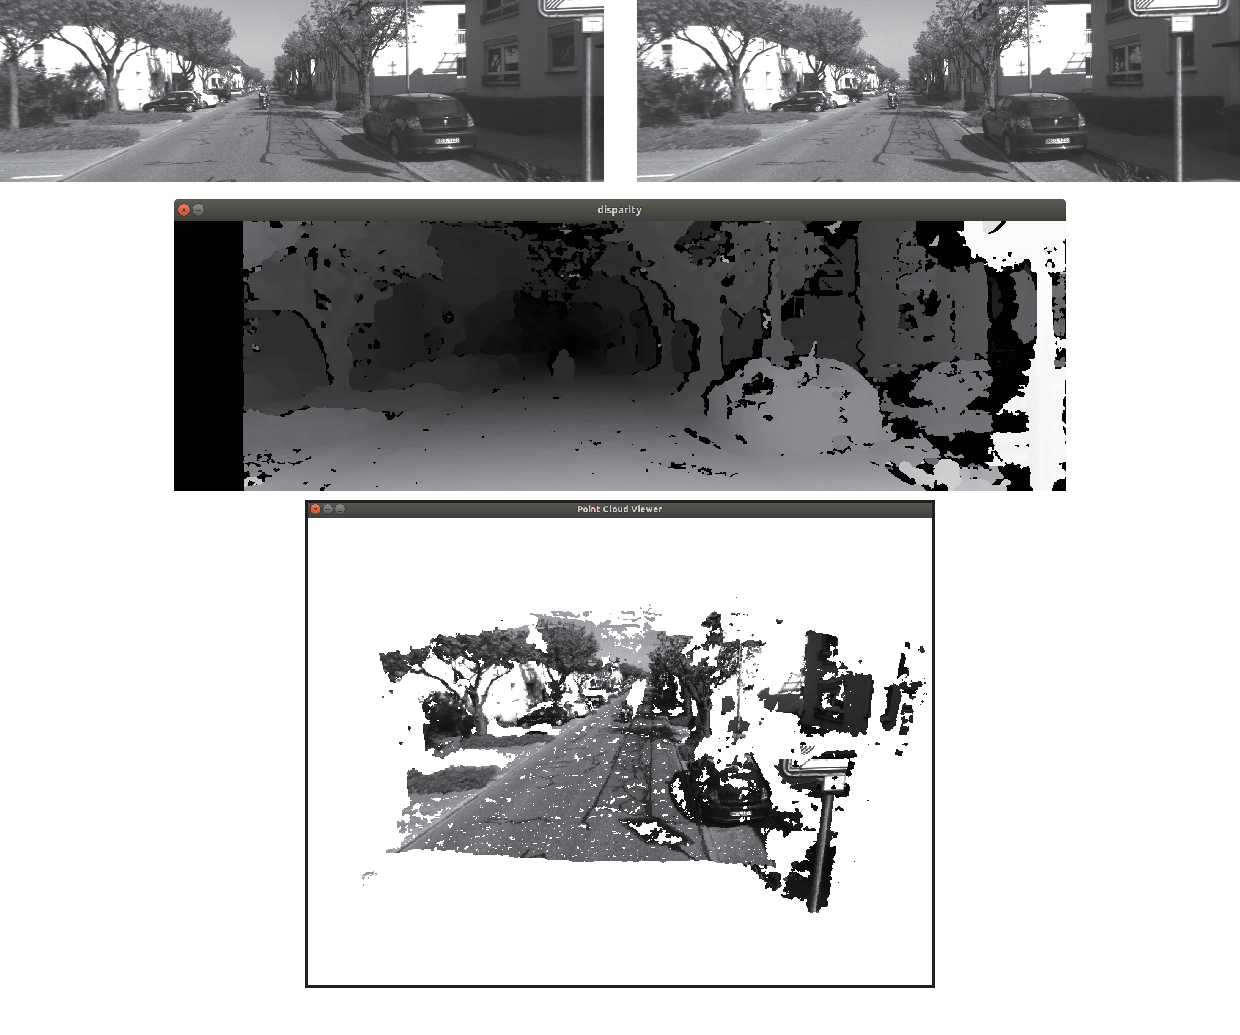
\includegraphics[width=0.9\textwidth]{cameraModel/stereoExample.pdf}
    \caption{Stereo image example. Top-left: left image, top-right: right image, mid: SGBM disparity map, bottom: point cloud. Note that since some of the pixels in the left image is not seen in the right one, so the disparity map will have some empty values.}
    \label{fig:stereoExample}
\end{figure}

In this example, we call the SGBM (Semi-global Batch Matching) {\cite{Hirschmuller2008}} algorithm implemented by OpenCV to calculate the disparity of the left and right images and then transform it into the 3D space of the camera through the geometric model of the binocular camera. We use a classic parameter configuration from the internet, and we mainly adjust the maximum and minimum disparity. The disparity data combined with the camera's internal parameters and baseline can determine each point's position in three-dimensional space. We omit the code related to displaying the point cloud to save some space.

This book is not going to introduce the disparity calculation algorithm of the binocular camera. Interested readers can read the relevant references {\cite{Scharstein2002, Seitz2006}}. In addition to the binocular algorithm implemented by OpenCV, there are many other libraries focused on achieving efficient parallax calculations. It is still an active and complex subject today.

\subsection{RGB-D Vision}
\label{sec:join-point-cloud}
Finally, we demonstrate an example of RGB-D vision. The convenience of RGB-D cameras is that they can obtain pixel depth information through physical methods. If the camera's intrinsic and extrinsic are known, we can calculate any pixel position in the world coordinate system, thereby creating a point cloud map. Now let's demonstrate how to do it.

We have prepared 5 pairs of images located in the slambook2/ch5/rgbd folder. There are 5 RGB images from 1.png to 5.png under the color/ directory and 5 corresponding depth images under the depth/. At the same time, the ``pose.txt'' file gives the camera poses of the 5 images (in the form of $ \mathbf{T}_\mathrm{wc} $). The format of the pose record is the same as before, with the translation vector plus a rotation quaternion:
\[
[x, y, z, q_x, q_y, q_z, q_w],
\]
where $q_w$ is the real part of the quaternion. For example, the parameters of the first pair of image are:
\[
[-0.228993, 0.00645704, 0.0287837, -0.0004327, -0.113131, -0.0326832, 0.993042].
\]

Below we write a program to accomplish two things: (1) We calculate the point cloud corresponding to each pair of RGB-D images based on internal parameters; (2) According to the camera pose of each image, we put the points to a global cloud by the camera poses.

\begin{lstlisting}[language=C++,caption=slambook/ch5/rgbd/jointMap.cpp (Part)]
int main(int argc, char **argv) {
    vector<cv::Mat> colorImgs, depthImgs;
    TrajectoryType poses;         // camera poses
    
    ifstream fin("./pose.txt");
    if (!fin) {
        cerr << "Please run the program in the directory that has pose.txt" << endl;
        return 1;
    }
    
    for (int i = 0; i < 5; i++) {
        boost::format fmt("./%s/%d.%s"); // the image format
        colorImgs.push_back(cv::imread((fmt % "color" % (i + 1) % "png").str()));
        depthImgs.push_back(cv::imread((fmt % "depth" % (i + 1) % "pgm").str(), -1)); // use -1 flag to load the depth image
        
        double data[7] = {0};
        for (auto &d:data) fin >> d;
        Sophus::SE3d pose(Eigen::Quaterniond(data[6], data[3], data[4], data[5]),
        Eigen::Vector3d(data[0], data[1], data[2]));
        poses.push_back(pose);
    }
    
    // compute the point cloud using camera intrinsics
    double cx = 325.5;
    double cy = 253.5;
    double fx = 518.0;
    double fy = 519.0;
    double depthScale = 1000.0;
    vector<Vector6d, Eigen::aligned_allocator<Vector6d>> pointcloud;
    pointcloud.reserve(1000000);
    
    for (int i = 0; i < 5; i++) {
        cout << "Converting RGBD images " << i + 1 << endl;
        cv::Mat color = colorImgs[i];
        cv::Mat depth = depthImgs[i];
        Sophus::SE3d T = poses[i];
        for (int v = 0; v < color.rows; v++)
        for (int u = 0; u < color.cols; u++) {
            unsigned int d = depth.ptr<unsigned short>(v)[u]; // depth value is 16-bit
            if (d == 0) continue; // 0 means no valid value
            Eigen::Vector3d point;
            point[2] = double(d) / depthScale;
            point[0] = (u - cx) * point[2] / fx;
            point[1] = (v - cy) * point[2] / fy;
            Eigen::Vector3d pointWorld = T * point;
            
            Vector6d p;
            p.head<3>() = pointWorld;
            p[5] = color.data[v * color.step + u * color.channels()];   // blue
            p[4] = color.data[v * color.step + u * color.channels() + 1]; // green
            p[3] = color.data[v * color.step + u * color.channels() + 2]; // red
            pointcloud.push_back(p);
        }
    }
    
    cout << "global point cloud has " << pointcloud.size() << " points." << endl;
    showPointCloud(pointcloud);
    return 0;
}
\end{lstlisting}

We can see the point cloud in \textit{Pangolin} after building it (see \autoref{fig:pointcloudmapping}).

\begin{figure}[!t]
    \centering
    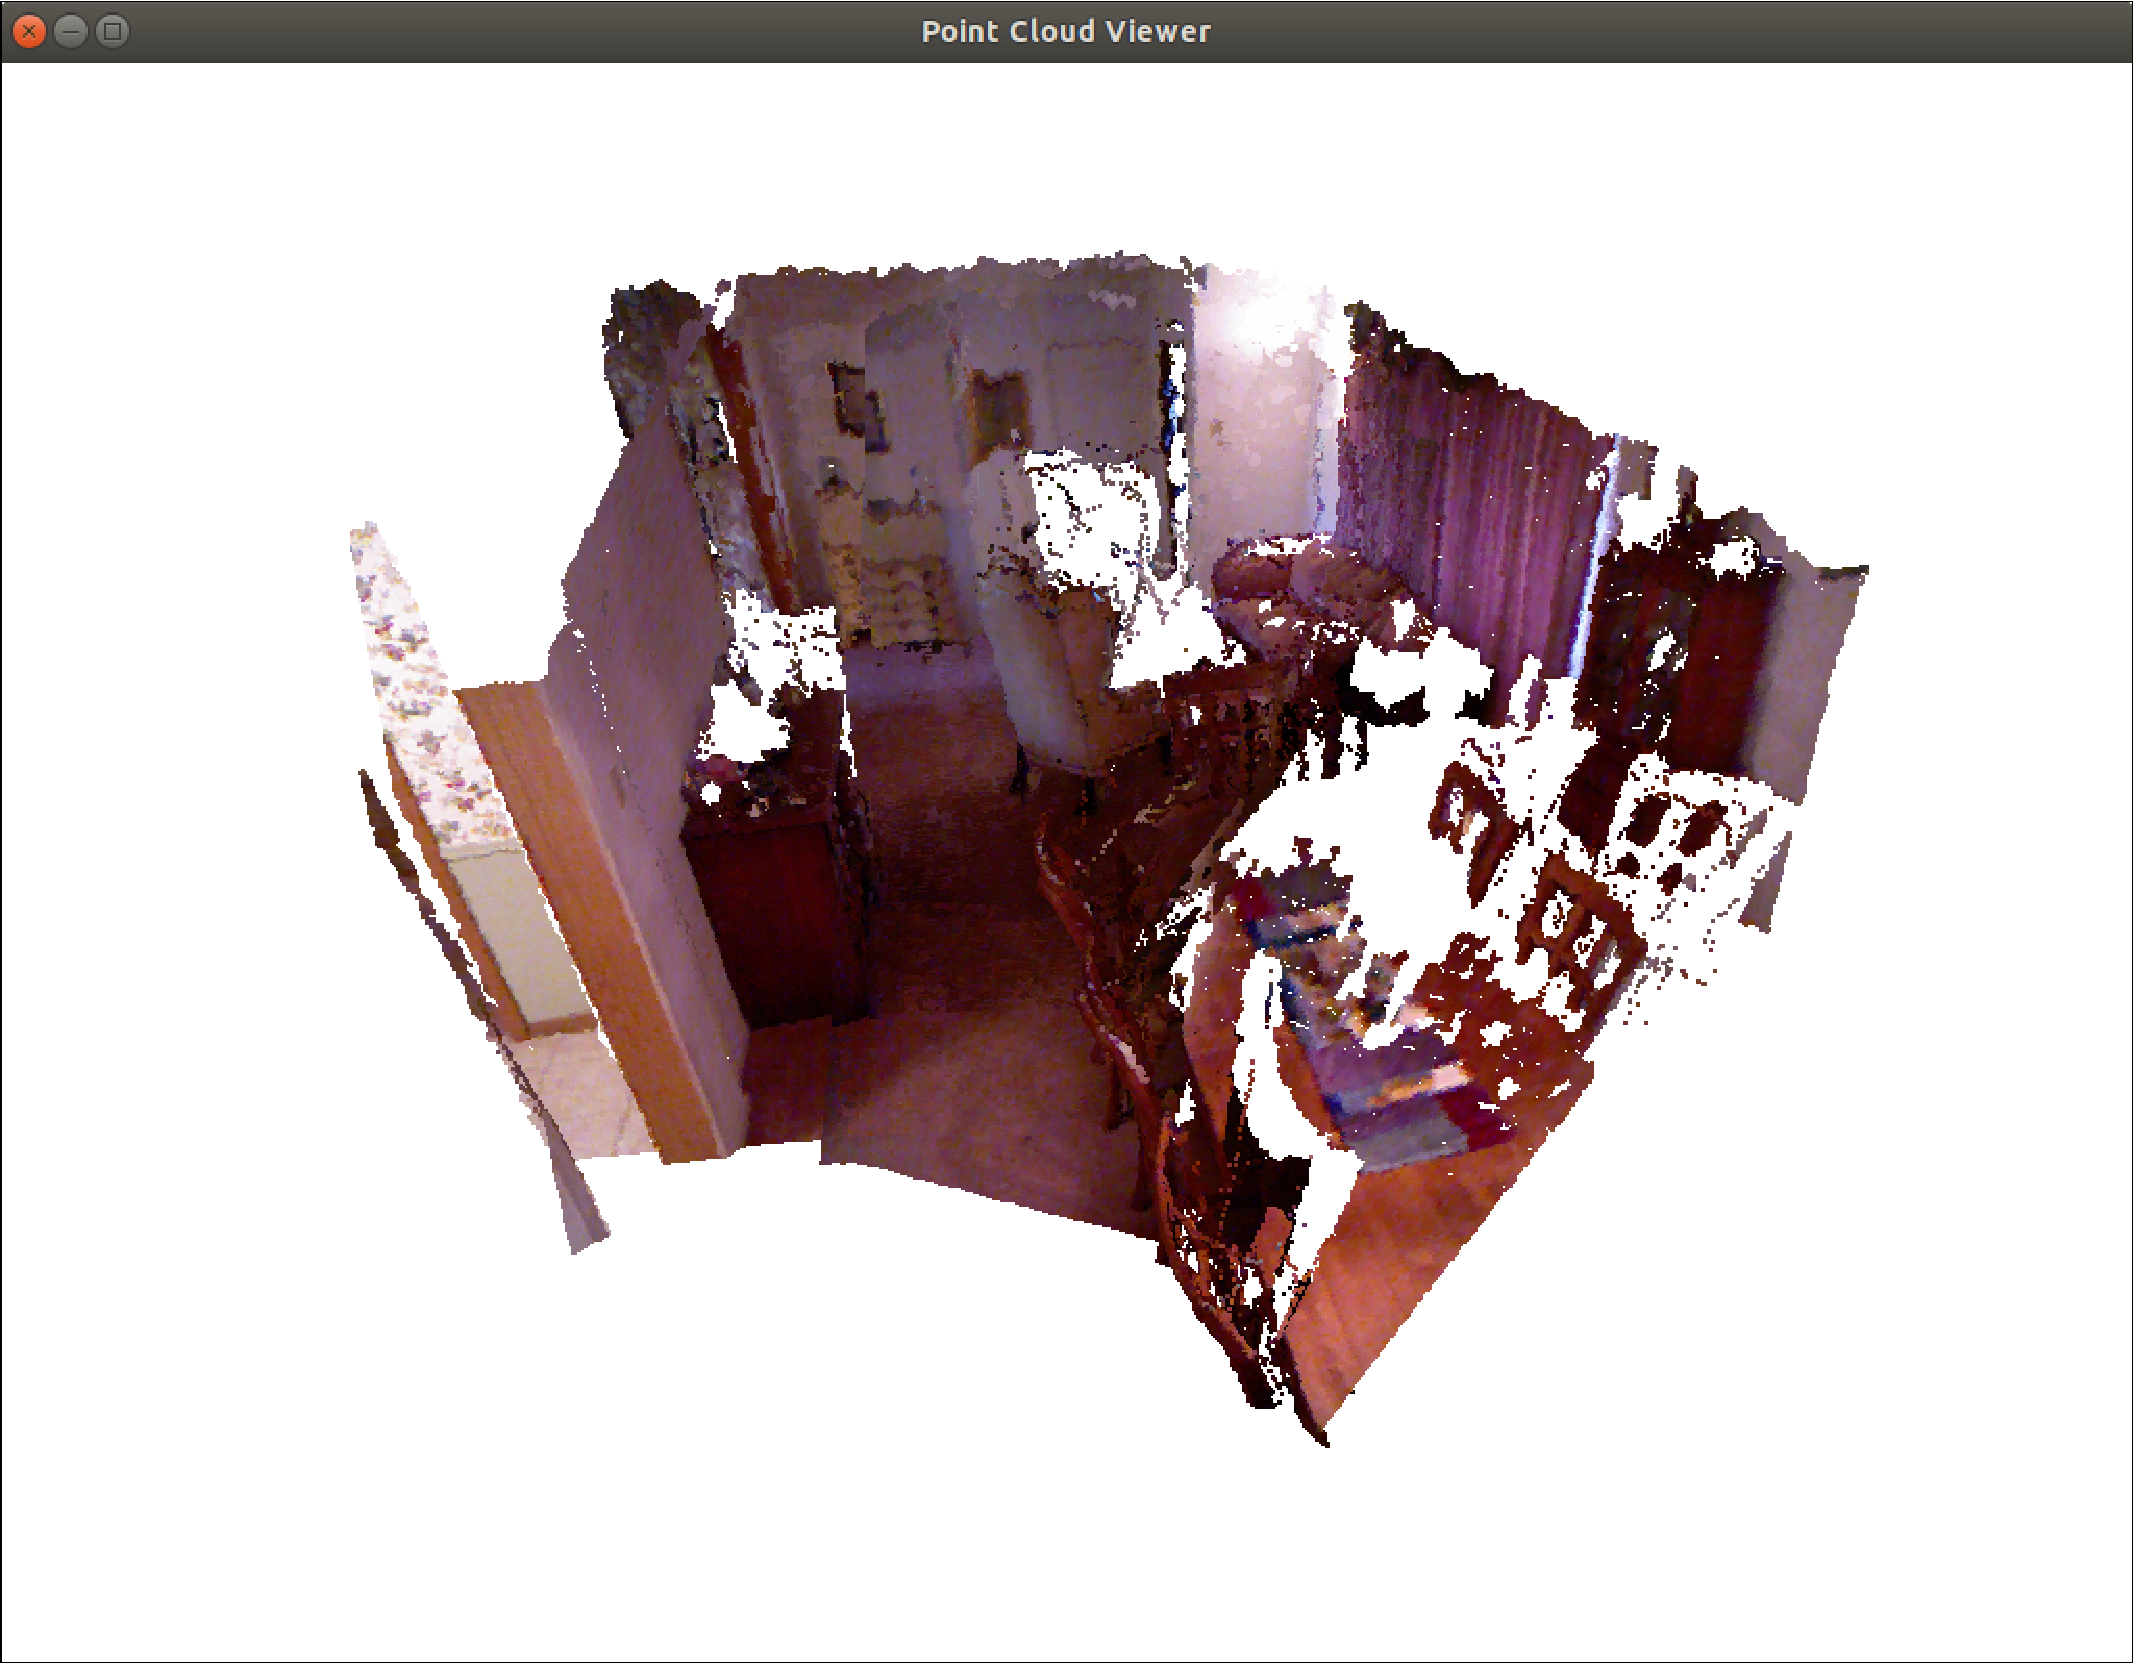
\includegraphics[width=1.0\textwidth]{cameraModel/pointcloud.pdf}
    \caption{The global point cloud from 5 RGBD image pairs.}
    \label{fig:pointcloudmapping}
\end{figure}

We demonstrated some common monocular, binocular, and rgbd camera algorithms in computer vision through these examples. We hope readers can understand the meaning of the intrinsics, extrinsics, and distortion model through them.

\section * {Exercise}
\begin{enumerate}
\item[\optional] Find a camera (use the camera of your mobile phone or laptop if you don't have one) and calibrate its internal parameters. You may use a calibration board or print out a checkerboard for calibration.
\item Describes the physical meaning of the camera's intrinsics. If the resolution of a camera is doubled and the rest is unchanged, how does its intrinsic change?
\item Search for the calibration method of special cameras (fisheye or panoramic cameras). Where are the differences between them and the pinhole models? 
\item Investigate the similarities and differences between a global shutter camera and a rolling shutter camera. What are their advantages and disadvantages in SLAM?
\item How are RGB-D cameras calibrated? Taking Kinect as an example, what parameters need to be calibrated? (Refer to \url{https://github.com/code-iai/iai_kinect2}.)
\item In addition to the way of traversing the image demonstrated by the sample program, what other methods can you give to traverse the image?
\item[\optional] Read the official OpenCV tutorial to learn its basic usage.
\end{enumerate}


% !Mode:: "TeX:UTF-8"
\chapter{Nonlinear Optimization}
\label{cpt:6}
\begin{mdframed}  
	\textbf{Goal of Study}
	\begin{enumerate}[labelindent=0em,leftmargin=1.5em]
		\item Understand how to form the batch state estimation problem into a least-square and how to solve the least-square problem.
		\item Understand the Gauss-Newton and Levenburg-Marquardt method and implement them.
		\item Learn how to use the Google Ceres and \textit{g2o} library to solve a least-square problem.
	\end{enumerate}
\end{mdframed} 

In the previous lectures, we introduced the motion and observation equations of the classic SLAM model. Now we know that the pose in the equation can be described by the transformation matrix and then optimized by Lie algebra. The observation equation is given by the camera imaging model, in which the internal parameter is fixed with the camera, and the external parameter is the pose of the camera. So, we have figured out the concrete expression of the classic visual SLAM model.

However, due to the presence of noise, the equations of motion and observation can not be exactly met. Although the camera can fit the pinhole model very well, unfortunately, the data we get is usually affected by various unknown noises. Even if we have a high-precision camera and controller, the motion and observations equations can only be approximated. Therefore, instead of assuming that the data must conform to the equation precisely, it is better to find an estimation approach to get the state from the noisy data.

Solving the state estimation problem requires a certain degree of optimization background knowledge. This section will introduce the basic unconstrained nonlinear optimization method and introduce optimization libraries \textit{g2o} and Ceres.

\newpage
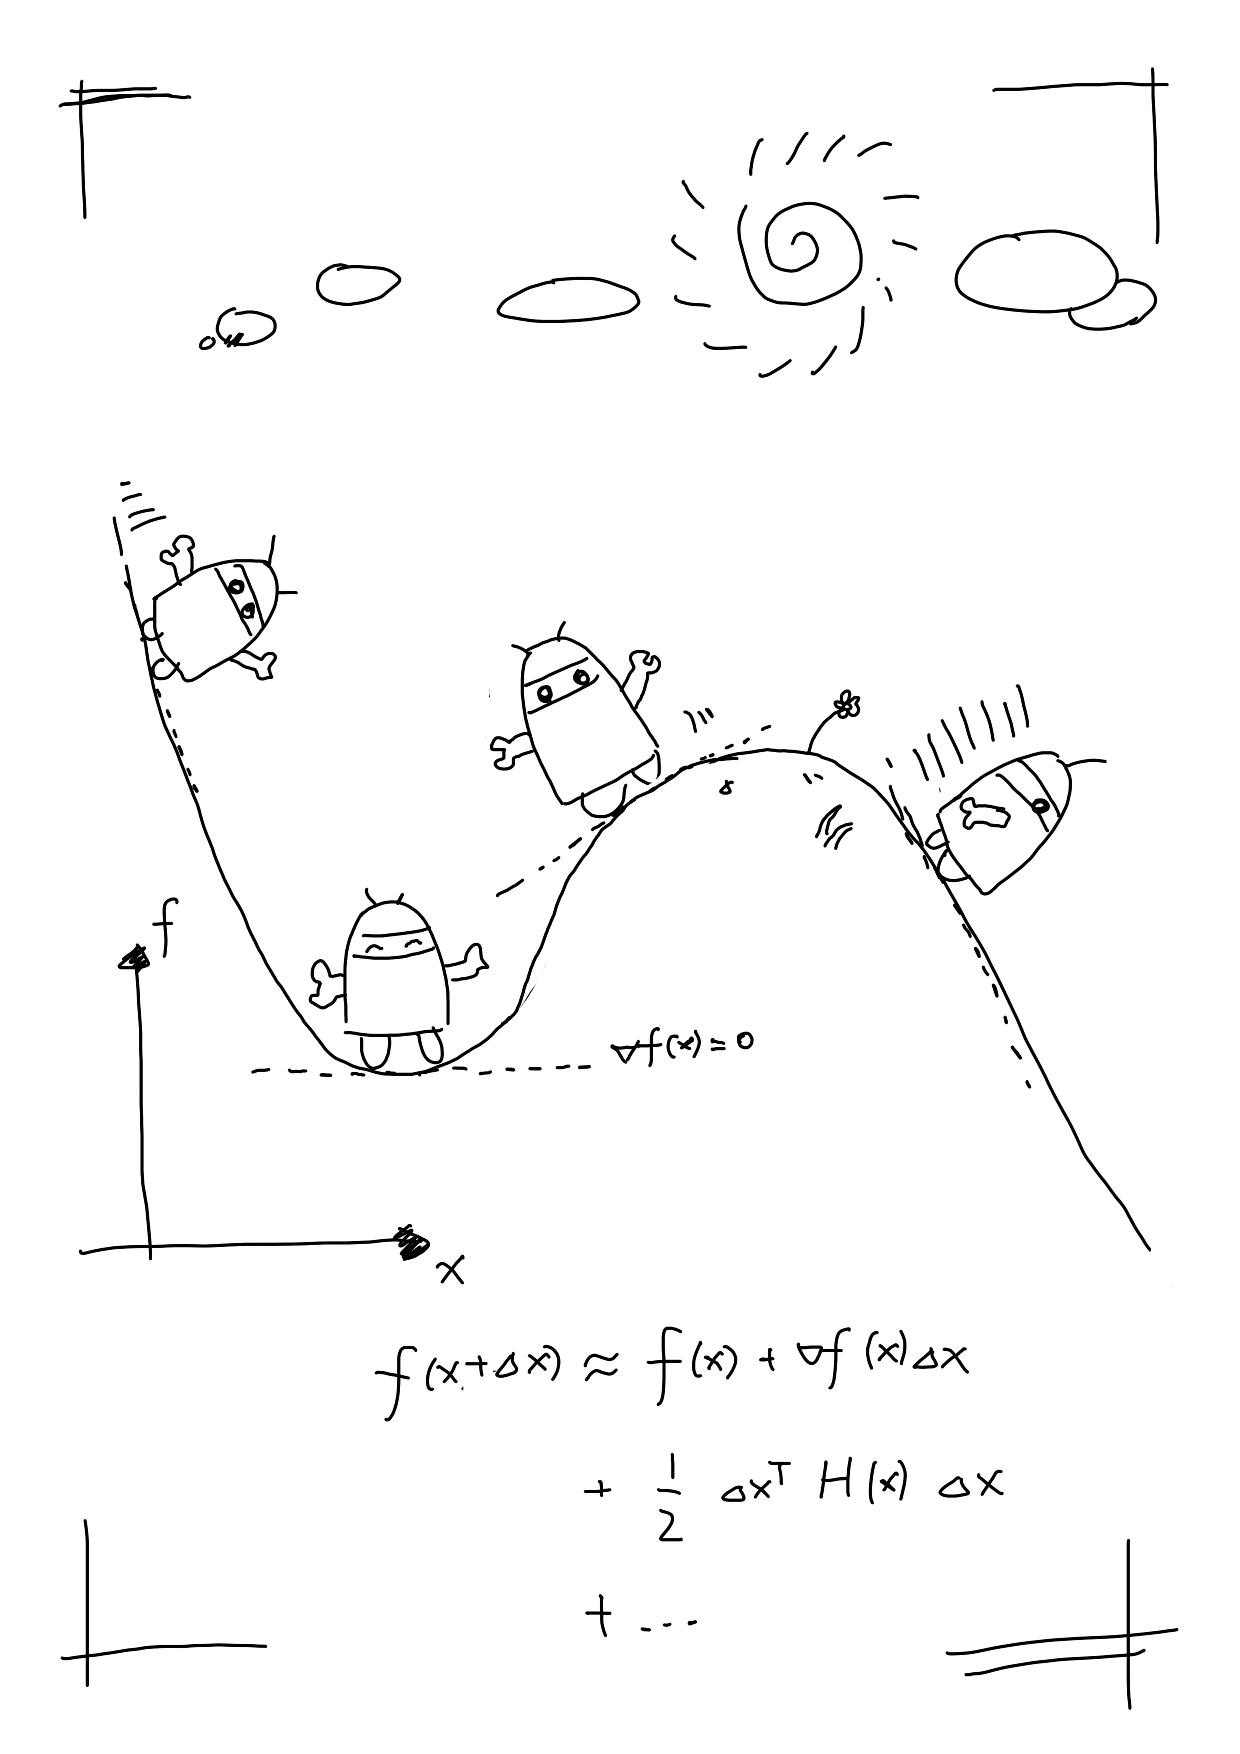
\includepdf{resources/other/ch6.pdf}

\newpage
\section{State Estimation}
\subsection{From Batch State Estimation to least-square}
According to the previous sections, the SLAM process can be described by a discrete-time motion and observation equations like~\eqref{eq:slamproblem}:
\begin{equation}
\left\{ \begin{array}{l}
{\mathbf{x}_k} = \mathbf{f}\left( {{\mathbf{x}_{k - 1}},{\mathbf{u}_k}} \right) + \mathbf{w}_k\\
{\mathbf{z}_{k,j}} = \mathbf{h}\left( {{ \mathbf{y}_j},{ \mathbf{x}_k}}  \right)+ \mathbf{v}_{k,j}
\end{array} \right. .
\end{equation}

Through the knowledge in lecture~\ref{cpt:4}, we learned that $ \mathbf {x} _k $ is the pose of the camera, which can be described by $ \mathrm {SE} (3) $. As for the observation equation, we have already explained in lecture~\ref{cpt:5} that it is just the pinhole camera model. To give readers a deeper impression of them, we may wish to discuss their specific parameterized form. First, the pose variable $\mathbf {x} _k $ can be expressed by $\mathbf {T} _k \in \mathrm {SE} (3) $. Second, the motion is related to the specific form of the input, but there is no particularity in visual SLAM (should be the same as ordinary robots and vehicles). We will not talk about it for now. The observation equation is given by the pinhole model. Assuming an observation of the road sign $ \mathbf {y} _j $ at $ \mathbf {x} _k $, corresponding to the pixel position on the image $ \mathbf {z} _ {k, j} $, then, observe The equation can be expressed as:
\begin{equation}
s \mathbf{z}_{k,j}= \mathbf{K} (\mathbf{R}_k {\mathbf{y}_j}+\mathbf{t}_k),
\end{equation}
where $ \mathbf {K} $ is the intrinsic matrix of the camera, and $s$ is the distance of pixels, which is also the third element of $ (\mathbf {R} _k {\mathbf {y} _j} + \mathbf {t} _k) $. If we use  transformation matrix $ \mathbf {T} _k $ to describe the pose, then the points $ \mathbf {y} _j $ must be described in homogeneous coordinates, and then converted to non-homogeneous coordinates afterwards. If you are not familiar with this process, please go back to the previous lectures.

Now, consider what happens when the data is affected by noise. In the motion and observation equations, we \textit {usually} assume that the two noise terms $ \mathbf {w} _k, \mathbf {v} _ {k, j} $ satisfy a Gaussian distribution with zero mean, like this:
\begin{equation}
{\mathbf{w}_k} \sim \mathcal{N}\left( {\mathbf{0},{\mathbf{R}_k}} \right),{\mathbf{v}_k} \sim \mathcal{N}\left( {\mathbf{0},{{{\mathbf{Q}}}_{k,j}}} \right),
\end{equation}
where $ \mathcal {N} $ means Gaussian distribution, $ \mathbf{0} $ means zero mean, and $ \mathbf {R} _k, \mathbf {Q} _ {k, j} $ is the covariance matrix. Under the influence of these noises, we hope to infer the pose $ \mathbf {x} $ and the map $ \mathbf {y} $ from the noisy data $ \mathbf {z} $ and $ \mathbf {u} $ (and their probability density distribution), which constitutes a state estimation problem.

Generally, there are two ways to deal with this state estimation problem. Since these data come gradually over time in the SLAM process, we should intuitively hold an estimated state at the current moment and then update it with new data. This method is called the \textit {incremental} method, or \textit{filtering}. For a long time in history, researchers have used filters, especially the extended Kalman filter (EKF) and its derivatives, to solve it. The other way is to record the data into a file and looking for the best trajectory and map in all time. This method is called the \textit {batch} estimation. In other words, we can collect all the input and observation data from time 0 to $ k $ together and ask, with such input and observation, how to estimate the entire trajectory and map from time 0 to $ k $?

These two different processing methods lead to many estimation methods. In general, the incremental method only cares about the state estimation of the \textit {current moment} $ \mathbf {x} _k $ but does not consider much about the previous state. Conversely, the batch method can be used to get an optimized trajectory in a long time, which is considered superior to the traditional filters~\cite {Strasdat2012}, and has become the mainstream method of current visual SLAM. In extreme cases, we can let robots or drones collect data and then bring it back to the computing center for unified processing, which is also the mainstream practice of SfM (structure from motion). Of course, in these cases, the method is obviously not \textit {real-time}, which is not the most common application scenario of SLAM. So in SLAM, practical methods are usually some compromises. For example, we fix some historical trajectories and only optimize some trajectories close to the current moment, leading to the sliding window estimation method described later.

In theory, the batch method is easier to introduce. At the same time, understanding the batch method also makes it easier to understand the incremental method. Therefore, in this section, we focus on the batch optimization method based on nonlinear optimization. The Kalman filter and more in-depth knowledge will be discussed in the backend chapter. Since the batch method is discussed, we will consider all the moments from time 1 to $N$ and assume $M$ map points. Define the robot pose and map coordinates at all times as:
\[
\mathbf{x}=\{ \mathbf{x}_1, \ldots, \mathbf{x}_N \}, \quad \mathbf{y} = \{\mathbf{y}_1, \ldots, \mathbf{y}_M \}.
\]
Similarly, $ \mathbf {u} $ without subscript is used for input at all times, and $ \mathbf {z} $ is used for observation data at all times. Then we say that the state estimation of the robot, from a probabilistic point of view, is to find the state $ \mathbf {x}, \mathbf{y}$ under the condition that the input data $ \mathbf {u} $ and the observation data $\mathbf{z} $. Or, the conditional probability distribution of:
\begin{equation}
P( \mathbf{x},\mathbf{y} | \mathbf{z}, \mathbf{u}).
\end{equation}


In particular, when we do not know the control input and only have one image, that is, only considering the data brought by the observation equation, it is equivalent to estimate the conditional probability distribution $ P (\mathbf {x}, \mathbf {y} | \mathbf { z}) $. Such a problem is also called Structure from Motion (SfM), that is, how to reconstruct the three-dimensional spatial structure from images only {\cite {Agarwal2009}}.

To estimation the conditional pdf, we use the Bayes equation to switch the variables:
\begin{equation}
P\left( { \mathbf{x},\mathbf{y}| \mathbf{z}, \mathbf{u}} \right) = \frac{{P\left( {\mathbf{z},\mathbf{u}|\mathbf{x},\mathbf{y}} \right)P\left( \mathbf{x}, \mathbf{y} \right)}}{{P\left( \mathbf{z},\mathbf{u}\right)}} \propto \underbrace{P\left(  { \mathbf{z},\mathbf{u}| \mathbf{x},\mathbf{y} } \right)}_{\text{likehood}} \underbrace{P\left( \mathbf{x},\mathbf{y} \right)}_{\text{prior}}.
\end{equation}

The left side is called \textit {posterior probability}, and $ P (\mathbf {z} | \mathbf {x}) $ on the right is called \textit {likelihood} (or likehood), and the other part is $ P (\mathbf {x}) $ is called \textit {prior}. \textit {It is normally difficult to find the posterior distribution directly (in nonlinear systems), but it is feasible to find an optimal point which maximize the posterior} (Maximize a Posterior, MAP):
\begin{equation}
{(\mathbf{x},\mathbf{y})^*}_{\mathrm{MAP}} = \arg {\mathop{\rm max}\nolimits} P \left( {\mathbf{x},\mathbf{y}|\mathbf{z},\mathbf{u}} \right) = \arg \max P(\mathbf{z},\mathbf{u}|\mathbf{x},\mathbf{y})P(\mathbf{x},\mathbf{y}).
\end{equation}

Please note that the denominator part of Bayes' rule has nothing to do with the state $ \mathbf {x}, \mathbf {y} $ to be estimated, so it can be just ignored. Bayes' rule tells us that solving the maximum posterior probability is \textit {equivalent to the estimate the product of maximum likelihood and a priori}. Further, we can also say, ``I'm sorry, I don't know in prior where the robot pose or the map points are'', then there is no \textit {prior}. In this case, we can solve the \textit {Maximize Likelihood Estimation} (MLE):
\begin{equation}
{ (\mathbf{x},\mathbf{y})^*}_{\mathrm{MLE}} = \arg \max P( \mathbf{z},\mathbf{u}| \mathbf{x},\mathbf{y}).
\end{equation}

Intuitively speaking, likelihood refers to ``what observation data may be generated in the current pose''. Since we know the observation data, the maximum likelihood estimation can be understood as: ``under what state, it is most likely to produce the data currently observed''. 

\subsection{Introduction to least-squares}
Now we have formulated the state estimation problem into a MAP/MLE problem, and the next question is how to solve it. Under the assumption of Gaussian distribution, we can have a simpler form of the maximum likelihood problem. Looking back at the observation model, for a certain kind of observation, we have:
\[
{\mathbf{z}_{k,j}} = h\left( {{ \mathbf{y}_j},{ \mathbf{x}_k}} \right)+ \mathbf{v}_{k, j},
\]
Since we assume the noise item is Gaussian, which means ${\mathbf{v}_k} \sim \mathcal{N}\left( {\mathbf{0},{{{\mathbf{Q}}}_{k,j}}} \right)$, so the conditional probability of the observation data is:
\[
P( \mathbf{z}_{j,k} | \mathbf{x}_k, \mathbf{y}_j) = N\left( h(\mathbf{y}_j, \mathbf{x}_k), \mathbf{Q}_{k,j} \right),
\]
which is, of course, still a Gaussian distribution. Now let's consider solving the maximum likelihood estimation under this single observation.

We can rewrite this maximum problem into a \textit{minimum of negative logarithm} one. Gaussian distributions have better mathematical forms under negative logarithm. Consider an arbitrary multi-dimensional Gaussian distribution $\mathbf{x} \sim \mathcal{N}(\mathbf{\mu}, \boldsymbol{\Sigma})$, its probability density function expansion form is:
\begin{equation}
	P\left( \mathbf{x} \right) = \frac{1}{{\sqrt {{{(2\pi )}^N}\det (\boldsymbol{\Sigma} )} }}\exp \left( {-\frac{1}{2}{{\left( {\mathbf{x}-\mathbf{\mu}} \right)}^T}{ \boldsymbol{\Sigma} ^ {-1}}\left( {\mathbf{x}-\mathbf{\mu}} \right)} \right).
\end{equation}
Take the negative logarithm of both sides:
\begin{equation}
	-\ln \left( {P\left( \mathbf{x} \right)} \right) = \underbrace{\frac{1}{2}\ln \left( {{{\left( {2\pi} \right )}^N}\det \left( \boldsymbol{\Sigma} \right)} \right)}_{\text{discarded}} + \frac{1}{2}{\left( {\mathbf{x}-\mathbf{\mu}} \right)^T}{\boldsymbol{\Sigma} ^{-1}}\left( {\mathbf{x}-\mathbf{\mu}} \right).
\end{equation}

Because the logarithm function is monotonically increasing, maximizing the original function is equivalent to minimizing the negative logarithm. When minimizing $\mathbf{x}$ in the above formula, the first term has nothing to do with $\mathbf{x}$ and can be omitted. Therefore, as long as the quadratic term on the right is minimized, the state's maximum likelihood estimate is obtained. Substituting into the SLAM observation model, it is equivalent to find such a solution:

\begin{equation}
	\begin{aligned}
		(\mathbf{x}_k,\mathbf{y}_j)^* &= \arg \max \mathcal{N}(h(\mathbf{y}_j, \mathbf{x}_k), \mathbf{Q }_{k,j}) \\ &= \arg \min \left( {{{\left( {{ \mathbf{z}_{k,j}}-h\left( {{\mathbf{x }_k},{\mathbf{y}_j}} \right)} \right)}^T} \mathbf{Q}_{k,j}^{-1}\left( {{\mathbf{z}_{k,j}}-h\left( {{\mathbf{x}_k},{\mathbf{y}_j}} \right)} \right)} \right).
	\end{aligned}
\end{equation}

We found that this equation is equivalent to a quadratic form that minimizes the noise term (i.e., the error). This quadratic form is called \textit{Mahalanobis distance}. It can also be regarded as the Euclidean distance ($\mathcal{L}_2$-norm) weighted by $\mathbf{Q}_{k,j}^{-1}$, where $\mathbf{Q}_{k,j} ^{-1}$ is also called the \textit{information matrix}, which is exactly the \textit{inverse} of the Gaussian covariance matrix.

Now we put all the observations together. It is usually assumed that the inputs and observations are independent of each other, which means that each input is independent, each observation is independent, and input and observation are still independent. So we can factorize the joint distribution like this:
\begin{equation}
	P\left( {\mathbf{z},\mathbf{u}|\mathbf{x},\mathbf{y}} \right) = \prod\limits_k {P\left( {{\mathbf{u}_k }|{\mathbf{x}_{k-1}},{\mathbf{x}_k}} \right)} \prod\limits_{k,j} {P\left( {{\mathbf{z} _{k,j}}|{\mathbf{x}_k},{\mathbf{y}_j}} \right)},
\end{equation}

It shows that we can handle the movement and observation at each moment independently. Let's define the error between the model and real data: 
\begin{equation}
	\begin{array}{l}
		{\mathbf{e}_{u,k}} = {\mathbf{x}_k}-f\left( {{\mathbf{x}_{k-1}},{\mathbf{u}_k} } \right)\\
		{\mathbf{e}_{z,j,k}} = {\mathbf{z}_{k,j}}-h\left( {{\mathbf{x}_k},{\mathbf{y} _j}} \right),
	\end{array}
\end{equation}
Then, minimizing the Mahalanobis distance between the estimated value and the measurements from sensors is equivalent to finding the maximum likelihood estimation. The negative logarithm allows us to turn the product into a summation:
\begin{equation}
	\label{eq:least-square}
	\min J (\mathbf{x},\mathbf{y}) = \sum\limits_k {\mathbf{e}_{u,k}^T \mathbf{R}_k^{-1} {\mathbf{e}_{u,k}}} + \sum\limits_k {\sum\limits_j {\mathbf{e}_{z,k,j}^T \mathbf{Q}_ {k,j}^{-1}{\mathbf{e}_{z,k,j}}}}.
\end{equation}
In this way, a \textit{least-square problem} is obtained with the same solution as the MLE problem. Intuitively speaking, due to the presence of noise, when we substitute the estimated trajectory and map into the SLAM motion and observation models, they will not be perfectly fit. What shall we do at this time? We perform \textit{fine-tuning} on the state's estimated value so that the overall error is reduced. Of course, finally, we will reach a (local) \textit{minimum value}. This is a typical nonlinear optimization process.

Observing the formula~\eqref{eq:least-square} carefully, we find that the least-squares problem in SLAM has some specific structures:

\begin{itemize}
	\item First, the objective function of the whole problem consists of many (weighted) error quadratic forms. Although the overall state variable's dimensionality is very high, each error term is simple and is only related to one or two state variables. For example, the motion error is only related to $\mathbf{x}_{k-1}, \mathbf{x}_k$, and the observation error is only related to $\mathbf{x}_k, \mathbf{y}_j$. This relationship will give a \textit{sparse} least-square problem, which we will investigate further in the backend chapter.
	\item Secondly, if you use Lie algebra to represent the increment, the problem is the least-squares problem of \textit{unconstrained}. However, if the rotation matrix/transformation matrix is used to describe the pose, the constraint of the rotation matrix itself will be introduced, that is, ``$\mathrm{s.t.}\ \mathbf{R}^T \mathbf{R} = \mathbf{I}$ and $\det (\mathbf{R})=1$ '' need to be added to the problem. Additional constraints can make optimization more difficult.
	\item Finally, we used a quadratic metric error, exactly the $\mathcal{L}_2-$norm. The information matrix is used as the weights of each element. For example, if an observation is very accurate, the covariance matrix will be ``small'' and the information matrix will be ``large'', so this error term will have a higher weight than the others in the whole problem. We will see some drawbacks of the $\mathcal{L}_2$ error later.
\end{itemize}

Next, we will introduce how to solve this least-squares problem, which requires some basic knowledge of nonlinear optimization. In particular, we want to discuss how to solve such a general unconstrained nonlinear least-squares problem. In the following lectures, we will make extensive use of this lecture's results and discuss its application in the SLAM's front and backends.

\subsection{Example: Batch State Estimation}
Maybe it's better to give an example here. Consider a very simple discrete-time system:
\begin{equation}
    \begin{array}{lll}
        {x_k} &= {x_{k-1}} + {u_k} + {w_k},&\qquad w_k \sim \mathcal{N}\left( {0,Q_k} \right)\\
        {z_k} &= {x_k} + {n_k},&\qquad {n_k}\sim \mathcal{N}\left( {0,R_k} \right)
    \end{array},
\end{equation}
which describes a car moving forward or backward along the $x$ axis. The first formula is the motion model, where $u_k$ is the input, and $w_k$ is the noise; the second formula is the observation model, where $z_k$ is the measurement of the position. We set the time $k=1,\ldots,3$, and want to estimate the states based on the existing $v,y$. Suppose the initial state $x_0$ is known. Let's derive the maximum likelihood estimation of the batch state estimation.

First, let the batch state variable be $\mathbf{x} = [x_0,x_1, x_2, x_3]^T$, and the batch observation be $\mathbf{z} = [z_1,z_2,z_3]^T$, define $\mathbf{u}=[u_1,u_2,u_3]^T$ in the same way. According to the previous derivation, we know that the maximum likelihood estimate is:
\begin{equation}
    \begin{aligned}
        {\mathbf{x}_{\mathrm{map}}^*} &= \arg \max P(\mathbf{x}|\mathbf{u},\mathbf{z}) = \arg \max P( \mathbf{u},\mathbf{z}|\mathbf{x})\\
        &= \prod\limits_{k = 1}^3 {P({u_k}|{x_{k-1}},{x_k})\prod\limits_{k = 1}^3 {P\left( { {z_k}|{x_k}} \right)} },
    \end{aligned}
\end{equation}
For each item, such as the motion equation, we have:
\begin{equation}
    P({u_k}|{x_{k-1}},{x_k}) = \mathcal{N}({x_k}-{x_{k-1}},{Q_k}).
\end{equation}
The observation equation is similar:
\begin{equation}
    P\left( {{z_k}|{x_k}} \right) = \mathcal{N}\left( {{x_k},{R_k}} \right).
\end{equation}
According to the previous statements, the error variable can be constructed as:
\begin{equation}
    {e_{u,k}} = {x_k}-{x_{k-1}}-{u_k}, \quad {e_{z,k}} = {z_k}-{x_k},
\end{equation}
Then the objective function of the least-squares is:
\begin{equation}
    \min \sum\limits_{k = 1}^3 {e_{u,k}^T Q_k^{-1}{e_{u,k}}} + \sum\limits_{k = 1 }^3 {e_{z,k}^T{R^{-1}_k}{e_{z,k}}}.
\end{equation}

In addition, since this system is a linear one, we can easily write the equations in the vector/matrix form. Define the vector $\mathbf{y}=[\mathbf{u}, \mathbf{z}]^T$, then the error can be defined as:
\begin{equation}
    \mathbf{y}-\mathbf{H}\mathbf{x} = \mathbf{e} \sim \mathcal{N}(\mathbf{0}, \boldsymbol{\Sigma}),
\end{equation}
where
\begin{equation}
    \mathbf{H} = \left[ {\begin{array}{*{20}{c}}
            1&{-1}&0&0\\
            0&1&{-1}&0\\
            0&0&1&{-1}\\
            \hline
            0&1&0&0\\
            0&0&1&0\\
            0&0&0&1
    \end{array}} \right],
\end{equation}
and $\boldsymbol{\Sigma}=\mathrm{diag}(Q_1, Q_2, Q_3, R_1, R_2, R_3)$. The whole question can be written as:
\begin{equation}
    \mathbf{x}^*_{\mathrm{map}} = \arg \min \mathbf{e}^T \boldsymbol{\Sigma}^{-1} \mathbf{e},
\end{equation}
Later we will see that this problem has a unique solution:
\begin{equation}
    \mathbf{x}^*_{\mathrm{map}} = (\mathbf{H}^T \boldsymbol{\Sigma}^{-1} \mathbf{H})^{-1} \mathbf{H}^T \boldsymbol{\Sigma}^{-1} \mathbf{y},
\end{equation}
since $(\mathbf{H}^T \boldsymbol{\Sigma}^{-1} \mathbf{H})^{-1}$ is invertible.

\section{Nonlinear Least-square Problem}
\label{sec:6.2}
First, consider a simple least-square problem:
\begin{equation}
    \mathop {\min }\limits_{\mathbf{x}} F(\mathbf{x}) = \frac{1}{2}{\left\| {f\left( \mathbf{x} \right) } \right\|^2_2},
\end{equation}
where the state variable is $\mathbf{x} \in \mathbb{R}^n$, and $f$ is any scalar nonlinear function $f(\mathbf{x}): \mathbb{R}^n \mapsto \mathbb{R}$. Note that the coefficient $\frac{1}{2}$ here is not important. Some literature has this coefficient, and some not. It will not affect the subsequent conclusions. Obviously, if $f$ is a mathematically simple function, then the problem can be solved in an analytical form. Let the derivative of the objective function be zero, and then find the optimal value of $\mathbf{x}$, just like finding the extreme value of a scalar function:
\begin{equation}
    \frac{ \mathrm{d} F}{ \mathrm{d} \mathbf{x}} = \mathbf{0}.
\end{equation}

We reach the minimum, maximum, or saddle points by solving this equation (or, intuitively, by letting the derivative be zero). But is this equation easy to solve? Well, it depends on the form of the derivative function of $f$. If $f$ is just a simple linear function, then the problem is only a simple linear least-square problem. But, some derivative functions may be complicated in form, making the equation difficult to solve. Solving this equation requires us to know the \textit{global property} of the objective function, which is usually not possible. For the least-square problem that is inconvenient to solve directly, we can use the \textit{iterated methods} to start from an initial value and continuously update the current estimations to reduce the objective function. The specific steps can be listed as follows:
\begin{mdframed}  
    \begin{enumerate}
        \item Give an initial value $\mathbf{x}_0$.
        \item For $k$-th iteration, we find an incremental value of $\Delta \mathbf{x}_k$, such that the object function $\left\| {f\left( \mathbf{x}_k + \Delta \mathbf{x}_k \right)} \right \|^2_2$ reaches a smaller value.
        \item If $\Delta \mathbf{x}_k$ is small enough, stop the algorithm.
        \item Otherwise, let $\mathbf{x}_{k+1} = \mathbf{x}_k+\Delta \mathbf{x}_k$ and return to step 2.
    \end{enumerate}
\end{mdframed}

Now things get much simpler. We turn the problem of solving the derivative function equals zero into a problem of looking for decreasing increments $\Delta \mathbf{x}_k$. We will see that since the objective function can be linearly approximated at the current estimation, the increment calculation will be more straightforward \footnote{Linear cases are always the easiest ones.}. When the function decreases until the increment becomes very small, it is considered that the algorithm converges, and the objective function reaches a minimum value. In this process, the problem is how to find the increment at each iteration point, which is a local problem. We only need to be concerned about the local properties of $f$ at the iteration value rather than the global properties. Such methods are widely used in optimization, machine learning, and other fields.

Next, we examine how to find this increment $\Delta \mathbf{x}_k$. This part of knowledge belongs to the field of numerical optimization. Let's take a quick look at some widely used results.

\subsection{The First and Second-order Method}
Now consider the $k$-th iteration. Suppose we are at $\mathbf{x}_k$ and want to find the increment $\Delta \mathbf{x}_k$, then the most intuitive way is to make the Taylor expansion of the objective function in $\mathbf{x}_k$:
\begin{equation}
    F(\mathbf{x}_k+\Delta \mathbf{x}_k) \approx F{\left( \mathbf{x}_k \right)} + \mathbf{J} \left( \mathbf{x}_k \right) ^T \Delta \mathbf{x}_k + \frac{1}{2}\Delta {\mathbf{x}_k^T}\mathbf{H}(\mathbf{ x}_k) \Delta \mathbf{x}_k,
\end{equation}
where $\mathbf{J}(\mathbf{x}_k)$ is the first derivative of $F(\mathbf{x})$ with respect to $\mathbf{x}$ (also called gradient, \textit{Jacobi} Matrix, or \textit{Jacobian}) \footnote{We write $\mathbf{J}(\mathbf{x})$ as a column vector, then it can be inner product with $\Delta \mathbf{x}$ to get a scalar. }, $\mathbf{H}$ is the second-order derivative (or \textit{Hessian}), which are all taken at $\mathbf{x}_k$. Readers should be familiar with them in the undergraduate course like multivariate calculus. We can choose to keep the first-order or second-order terms of the Taylor expansion, and the corresponding solution is called the first-order or the second-order method. In the simplest way, if we only keep the first-order one, then taking the increment at the minus gradient direction will ensure that the function decreases: 
\begin{equation}
    \Delta \mathbf{x}^* =-\mathbf{J}(\mathbf{x}_k).
\end{equation}

Of course, this is only a direction. Usually, we have to compute another step length parameter, say, $\lambda$. The step length can be calculated according to certain conditions {\cite{Wolfe1969}}. There are also some empirical methods in machine learning, but we will not discuss them. This method is called \textit{steepest descent method}. Its intuitive meaning is very simple. As long as we move along the reverse gradient direction, the objective function must decrease if the first-order (linear) approximation still holds.

Note that the above discussion was carried out during the $k$-th iteration and did not involve any information about $k$. To simplify the notation, we will omit the subscript $k$ later and think that these discussions are valid for each iteration.

On the other hand, we can choose to keep the second step information, and the increment equation is:
\begin{equation}
    \Delta \mathbf{x}^* = \arg \min \left(F\left( \mathbf{x} \right) + \mathbf{J} \left( \mathbf{x} \right)^T \Delta \mathbf{x} + \frac{1}{2}\Delta {\mathbf{x}^T}\mathbf{H} \Delta \mathbf{x} \right).
\end{equation}
The right side only contains the zero-order, first-order and quadratic terms of $\Delta \mathbf{x}$. Finding the derivative of $\Delta \mathbf{x}$ on the right side of the equation and setting it to zero leads to: \footnote{For students who are not familiar with matrix derivation, please refer to appendix~\ref{cpt:app-B}. }
\begin{equation}
    \label{eq:newton-method}
    \mathbf{J} + \mathbf{H} \Delta \mathbf{x} = \mathbf{0} \Rightarrow
    \mathbf{H} \Delta \mathbf{x} = -\mathbf{J}.
\end{equation}

We can also solve this linear equation and get the increment. This method is also called \textit{Newton's method}.

We have seen that both the first-order and second-order methods are very intuitive, as long as we can calculate the Taylor expansion of $f$ and find the increments. We say, hey, the function looks like a linear or quadratic one. We can use the approximated function's minimum value to guess the minimum value of the original function. As long as the original objective function really looks like a first-order or quadratic function locally, this type of algorithm is always valid (this is also the most cases in reality). However, these two methods also have their drawbacks. The steepest descent method is too greedy and easy to lead a zigzag way and increases the number of iterations. However, Newton's method needs to calculate the $\mathbf{H}$ matrix of the objective function, which is very time-expensive when the problem is large. We usually tend to avoid the calculation of $\mathbf{H}$. For general problems, some quasi-Newton methods can get better results. For least-square problems, there are several more practical methods: the \textit{Gauss-Newton's method} and the (Levernburg-Marquardt's method).

\subsection{The Gauss-Newton Method}
The Gauss-Newton method is one of the simplest methods in optimization algorithms. Its idea is to carry out a first-order Taylor expansion of $f(\mathbf{x})$. Please note that this is not the objective function $F(\mathbf{x})$ but the lower case $f(\mathbf{x})$, otherwise it is the same as Newton's method.
\begin{equation}
    \label{eq:approximation}
    f\left( {\mathbf{x} + \Delta \mathbf{x}} \right) \approx f\left( \mathbf{x} \right) + \mathbf{J} \left( \mathbf{x} \right)^T \Delta \mathbf{x}.
\end{equation}

Here $\mathbf{J}(\mathbf{x})$ is the derivative of $f(\mathbf{x})$ with respect to $\mathbf{x}$, which is a column vector of $n \times 1$. According to the previous framework, the current goal is to find the increment $\Delta \mathbf{x}$ such that $\left\| {f\left( \mathbf{x} + \Delta \mathbf{x} \right)} \right \|^2$ reached the minimum. In order to find $\Delta \mathbf{x}$, we need to solve a linear least-square problem \footnote{We omit the information matrix to simplify the derivation here.}:
\begin{equation}
    \Delta \mathbf{x}^* = \arg \mathop {\min }\limits_{\Delta \mathbf{x}} \frac{1}{2}{\left\| {f\left( \mathbf{x} \right) + \mathbf{J} \left( \mathbf{x} \right)^T \Delta \mathbf{x} } \right\|^2}.
\end{equation}
    
What's the difference from before? According to the extreme conditions, we set the derivative with $\Delta \mathbf{x}$ to zero to reach the extreme value. To do this, let's first expand the square term of the objective function:
\begin{align*}
    \frac{1}{2}{\left\| {f\left( \mathbf{x} \right) + \mathbf{J} \left( \mathbf{x} \right)^T \Delta \mathbf{x}} \right\|^2} &= \frac{1}{2}{\left( {f\left( \mathbf{x} \right) + \mathbf{J}\left( \mathbf{x} \right)^T \Delta \mathbf{x}} \right)^T}\left( {f\left( \mathbf{x} \right) + \mathbf{J} \left( \mathbf{x} \right)^T \Delta \mathbf{x}} \right)\\
    &= \frac{1}{2}\left( \| f{{\left( \mathbf{x} \right)}\|^2_2 + 2 f\left( \mathbf{x} \right) \mathbf{J} {{\left( \mathbf{x} \right)}}^T \Delta \mathbf{x} + \Delta { \mathbf{x}^T}{\mathbf{J} (\mathbf{x})} \mathbf{J}(\mathbf{x})^T \Delta \mathbf{x}} \right).
\end{align*}


Find the derivative of the above formula with respect to $\Delta \mathbf{x}$ and set it to zero:
\begin{displaymath}
    \mathbf{J} {\left( \mathbf{x} \right)}f\left( \mathbf{x} \right) + \mathbf{J} {\left( \mathbf{x} \right)} \mathbf{J}^T \left( \mathbf{x} \right)\Delta \mathbf{x} = \mathbf{0}.
\end{displaymath}

The following equation can be obtained:
\begin{equation}
    \underbrace{\mathbf{J} {\left( \mathbf{x} \right)} \mathbf{J}^T}_{\mathbf{H}(\mathbf{x})} \left( \mathbf{x} \right)\Delta \mathbf{x} =  \underbrace{- \mathbf{J} {\left( \mathbf{x} \right)} f\left( \mathbf{x} \right)}_{\mathbf{g}(\mathbf{x})}.
\end{equation}

This equation is a \textit{linear equation} of the variable $\Delta \mathbf{x}$. We call it \textit{normal equation} or \textit{Gauss-Newton equation}. We define the coefficients on the left as $\mathbf{H}$ and the coefficient on the right as $\mathbf{g}$, then the above formula becomes:
\begin{equation}
    \label{eq:minimize-deltax}
    \mathbf{H} \Delta \mathbf{x} = \mathbf{g}.
\end{equation}
It makes sense to mark the left side as $\mathbf{H}$ here. Compared with Newton's method~\ref{eq:newton-method}, Gauss-Newton's method uses $\mathbf{J}\mathbf{J}^T$ \textit{as the approximation} of the second-order Hessian matrix in Newton's method, thus omitting the calculation of $\mathbf{H}$. Please note that solving the normal equation is the core of the entire optimization problem. If we can get the $\Delta \mathbf{x}$ in each iteration, then the algorithm of the Gauss-Newton method can be written as:

\begin{mdframed}
    \begin{enumerate}
        \item Set it initial value as $\mathbf{x}_0$.
        \item For $k$-th iteration, calculate the Jacobian $\mathbf{J}(\mathbf{x}_k)$ and residual $f(\mathbf{x}_k)$.
        \item Solve the normal equation: $\mathbf{H} \Delta \mathbf{x}_k = \mathbf{g}$.
        \item If $\Delta \mathbf{x}_k$ is small enough, stop the algorithm. Otherwise let $\mathbf{x}_{k+1} = \mathbf{x}_k+\Delta \mathbf{x}_k$ and return to step 2.
    \end{enumerate}
\end{mdframed}

It can be seen from the algorithm steps that the solution of the incremental equation occupies the major position. As long as we can solve the increment smoothly, we can ensure that the objective function decreases correctly.

In order to solve the incremental equation, we need to solve $\mathbf{H}^{-1}$, which requires the $\mathbf{H}$ matrix to be invertible. However, the calculated $\mathbf{J} \mathbf{ J}^T$ is only semi-positive definite. If $\mathbf{J}$ has null-spaces, which means we can find non-zero $\Delta \mathbf{x}$ such that $\mathbf{J} \Delta\mathbf{x} = \mathbf{0}$, then we can not determine which $\Delta \mathbf{x}$ can really makes the objective function decreases. In that case, the algorithm is probably not converging, and we may obtain erroneous results. Intuitively, the local approximation of the original function at this point is not like a quadratic function. Furthermore, even if we assume that $\mathbf{H}$ is not singular or ill-conditioned, but if we take a very large step size $\Delta \mathbf{x}$, the result can still be bad since linear approximation is not accurate enough at that point. So in practice, we can't guarantee that the Gauss-Newton method converges. Sometimes they can reach even larger objective function values than the initial one. 

Although the Gauss-Newton method has these shortcomings, it is still a simple and effective method for nonlinear optimization, and it is worth learning. In nonlinear optimization, quite a lot of algorithms can be taken as the Gauss-Newton method's variants. These algorithms all use the idea of the Gauss-Newton method and correct their shortcomings through their own improvements. For example, some \textit{line search method} adds an extra step size $\alpha$. After determining $\Delta \mathbf{x}$, we may further find the $\alpha$ to make $\left\| f (\mathbf{x} + \alpha \Delta \mathbf{ x}) \right\|^2$ is minimized, instead of simply making $\alpha = 1$.

The Levenberg-Marquardt method corrects these problems to a certain extent. It is generally considered more robust than the Gauss-Newton method, but its convergence rate may be slower than the Gauss-Newton method. Such a kind of method is also called as \textit{damped Newton Method}.

\subsection{The Levernberg-Marquatdt Method}
The approximate second-order Taylor expansion used in the Gauss-Newton method can only have a good approximation effect near the expansion point. So, we naturally thought a range should be added to $\Delta \mathbf{x}$, called \textit{trust-region}. This range defines under what circumstances the second-order approximation is valid. This type of method is also called \textit{trust-region method}. We think the approximation is valid only in the trusted region; otherwise, it may go wrong if the approximation goes outside.

So how to determine the scope of this trust-region? A good method is to determine it based on the difference between our approximate model and the real object function: if the difference is small, it means that the approximation is good, and we may expand the trust-region; conversely, if the difference is large, we will reduce the range of approximation. We define an indicator $\rho$ to describe the degree of approximation:
\begin{equation}\label{eq:6.24}
	\rho = \frac{{f\left( {\mathbf{x} + \Delta \mathbf{x}} \right)}-{{ {f\left( \mathbf{x} \right)} }}} {\mathbf{J}\left( \mathbf{x} \right)^T \Delta \mathbf{x}}.
\end{equation}
The numerator of $\rho$ is the decreasing value of the real object function, and the denominator is the decreasing value of the approximate model. If $\rho$ is close to 1, we may say the approximation is good. A small $\rho$ is indicating that the actual reduced value is far less than the approximate reduced value. The approximation is poor in this case, and the trust-region needs to be reduced. Conversely, if $\rho$ is relatively large, it means that the actual decline is greater than expected, and we can enlarge the approximate range.

Therefore, we build an improved version of the nonlinear optimization framework, which will have a better effect than the Gauss-Newton method:

\begin{mdframed}
	\begin{enumerate}
		\item Give the initial value $\mathbf{x}_0$ and initial trust-region radius $\mu$.
		\item For $k$-th iteration, we solve a linear problem based on Gauss-Newton's method added with a trust-region: 
		\begin{equation}\label{eq:LM}
			\mathop {\min }\limits_{\Delta \mathbf{x}_k} \frac{1}{2}{\left\| {f\left( \mathbf{x}_k \right) + \mathbf{J} \left( \mathbf{x}_k \right)^T \Delta \mathbf{x}_k} \right\|^2}, \quad \mathrm{s.t.}\quad {\left\| {\mathbf{D} \Delta \mathbf{x}_k} \right\|^2} \leqslant \mu ,
		\end{equation}
		where $\mu$ is the radius and $\mathbf{D}$ is a coefficient matrix, which will be discussed in below. 
		\item Compute $\rho$ using equation \eqref{eq:6.24}. 
		\item If $\rho > \frac{3}{4}$, set $\mu = 2 \mu$. 
		\item Otherwise, if $\rho < \frac{1}{4}$, set $\mu = 0.5 \mu$. 
		\item If $\rho$ is larger than a given threshold, set $\mathbf{x}_{k+1} = \mathbf{x}_k+\Delta \mathbf{x}_k$. 
		\item Go back to step 2 if not converged, otherwise return the result. 
	\end{enumerate}
\end{mdframed}

Here, the range expansion's multiply factor and thresholds are empirical values and can be replaced with other values. In the formula \eqref{eq:LM}, we limit the increment to a sphere with a radius of $\mu$ and think that it is valid only in this sphere. After bringing into the $\mathbf{D}$, this sphere can be seen as an ellipsoid. In the optimization method proposed by Levenberg, taking $\mathbf{D}$ into the unit matrix $\mathbf{I}$ is equivalent to directly constraining $\Delta \mathbf{x}_k$ in a sphere. Subsequently, Marquardt proposed to take $\mathbf{D}$ as a non-negative diagonal matrix. In practice, the square root of the diagonal elements of $\mathbf{J}^T \mathbf{J}$ is usually used as $\mathbf{D}$ so that the constraint range is larger on the dimensions with small gradient.

In any case, in Levenberg-Marquardt optimization, we need to solve a sub-problem like \eqref{eq:LM} to obtain the gradient. This sub-problem is an optimization problem with inequality constraints. We use Lagrangian multipliers to put the constraints in the objective function to form the Lagrangian function:
\begin{equation}
    \mathcal{L}(\Delta \mathbf{x}_k, \lambda)= \frac{1}{2} {\left\| {f\left( \mathbf{x}_k \right) + \mathbf{J} \left( \mathbf{x}_k \right)^T \Delta \mathbf{x}_k} \right\|^2} + \frac{\lambda}{2} \left( \left\| \mathbf{D} \Delta \mathbf{x}_k \right\|^2 - \mu \right),
\end{equation}
where $\lambda$ is the Lagrange multiplier. Similar to the method in the Gauss-Newton, let the derivative of the Lagrangian function with respect to $\Delta \mathbf{x}$ be zero, and we still need to solve the linear equation for calculating the increment:
\begin{equation}
    \left( \mathbf{H} +\lambda \mathbf{D}^T \mathbf{D} \right) \Delta \mathbf{x}_k = \mathbf{g}.
\end{equation}

It can be seen that the incremental equation has an extra $\lambda \mathbf{D}^T \mathbf{D}$ compared to the Gauss-Newton method. If you consider its simplified form $\mathbf{D}=\mathbf{I}$, then it is equivalent to solving \footnote{Strict readers may not be satisfied with the description here. In addition to the Lagrangian function derivation to zero, the KKT condition also has some other constraints: $\lambda>0$, and $\lambda(\|\mathbf{D} \Delta \mathbf{x}\|^2-\mu)=0$. But in the L-M iteration, we might as well regard it as a penalty term (augmented Lagrangian) with $\lambda$ as the weight on the objective function of the original problem. After each iteration, if the trust-region condition is not satisfied, or the objective function increases, the weight of $\lambda$ is increased until the trust-region condition is finally satisfied. Therefore, there are different interpretations of the L-M algorithm in theory, but we only care about whether it works smoothly in practice. }:
\begin{displaymath}
    \left( \mathbf{H} +\lambda \mathbf{I} \right) \Delta \mathbf{x}_k = \mathbf{g}.
\end{displaymath}

We can see that when the parameter $\lambda$ is relatively small, $\mathbf{H}$ dominates the normal equation, which shows that the quadratic approximation model is better in this range. The Levenberg-Marquardt method is more close to the Gauss-Newton method. On the other hand, when $\lambda$ is relatively large, $\lambda \mathbf{I}$ occupies a dominant position. The Levenberg-Marquardt method is closer to the one-step descent method (the steepest descent), which means that the quadratic approximation is not good enough. The solution method of the Levenberg-Marquardt method can avoid the non-singular and ill-conditioned problems of the coefficient matrix of linear equations to a certain extent and provide more stable and accurate increments $\Delta \mathbf{x} $.

In practice, there are also many other ways to solve the increment, such as Dog-Leg~\cite{Nocedal2006} and other methods. What we have introduced here is just the most common and basic method, and it is also the most widely-used method in visual SLAM. We usually choose one of the Gauss-Newton or Levenberg-Marquardt methods as the gradient descent strategy in practical problems. When the problem is well-formed, Gauss-Newton is used. Otherwise, in ill-formed problems, we use the Levenberg-Marquardt method.

\subsection{Conclusion}
Since I don't want this book to become a headache-inducing mathematics textbook, only two of the most common nonlinear optimization schemes are listed here: the Gauss-Newton method and the Levenberg-Marquardt method. We avoided many discussions of mathematical properties. If readers are interested in optimization, you can read other books dedicated to numerical optimization (this is a big topic) like~\cite{Nocedal2006}. The optimization methods represented by the Gauss-Newton method and the Levenberg-Marquardt method have been implemented and provided to users in many open-source optimization libraries. We will conduct experiments below. Optimization is an essential mathematical tool for dealing with many practical problems. It plays a central role in visual SLAM and one of the core methods for solving problems in other fields such as deep learning (the amount of deep learning data is substantial, where the first-order method is a major choice). We hope that readers can learn more about optimization algorithms based on their own capabilities.

Perhaps you have discovered that whether it is the Gauss-Newton method or the Levenberg-Marquardt method, the variable's initial value needs to be provided when doing the optimization calculation. You may ask, can this initial value be set arbitrarily? Of course not. In fact, iterative solutions of nonlinear optimization require users to provide a good initial value. Because the objective function is too complicated, it is difficult to predict the solution space change. Providing different initial values for the problem often leads to different calculation results. This situation is a common problem of nonlinear optimization: most algorithms easily fall into local minima. Therefore, no matter what kind of scientific problem, we should provide the initial value carefully. For example, in the visual SLAM problem, we will use ICP, PnP, and other algorithms to provide the optimized initial value. In short, a good initial value is significant for optimization problems!

Readers may also have questions about the optimization mentioned above: how to solve the incremental linear equations? We have only mentioned that the incremental equation is linear, but does it require many calculations to invert the coefficient matrix directly? Of course not. In the visual SLAM algorithm, the dimension of $\Delta \mathbf{x}$ is often as large as hundreds or thousands. If you are doing large-scale visual 3D reconstruction, you will often find that this dimension can be easily achieved at hundreds of thousands or even higher levels. Most processors cannot afford such a large matrix inversion computation, so there are many numerical solutions for linear equations. There are different solutions in different fields, but there is almost no way to directly find the general inverse coefficient matrix. We will use matrix decomposition to solve linear equations, such as QR, Cholesky, and other decomposition methods. These methods can usually be found in textbooks, such as the matrix theory, and we will not introduce them.

Fortunately, the visual SLAM matrix has a specific sparse form, which can be solved in real-time applications. We will introduce its principle in detail in lecture~\ref{cpt:backend1}. Using the sparse form of elimination, decomposition, and finally solving increment will significantly improve the solution's efficiency. In many open source optimization libraries, variables with a dimension of more than 10,000 can be solved in a few seconds or less on a general PC. The reason is that more advanced mathematical tools are used. The visual SLAM algorithm can now be implemented in real-time, thanks to the coefficient matrix is sparse. If the matrix is dense, I am afraid that optimization of this kind of visual SLAM algorithm will not be widely adopted by the academic community~\cite{Lourakis2009, Sibley2009a, Triggs2000}.

\section{Practice: Curve Fitting}
\subsection{Curve Fitting with Gauss-Newton}
Next, we use a simple example to demonstrate how to solve the least-square problem. We will demonstrate how to write the Gauss-Newton method by hand and then introduce how to use the optimization library to solve this problem. For the same problem, these implementations will get the same result because their core algorithms are the same.

Consider a curve that satisfies the following equation:
\[
y = \exp( ax^2 + bx + c ) + w,
\]
where $a, b, c$ are the parameters of the curve, and $w$ is the Gaussian noise, satisfying $w \sim (0, \sigma^2)$. We deliberately chose such a nonlinear model so that the problem is not too easy. Now, suppose we have $N$ observation data points about $x and y$ and want to find the parameters of the curve based on these data points. Then, we solve the following least-square problem to estimate the curve parameters:
\begin{equation}
    \min \limits_{a,b,c} \frac{1}{2}\sum\limits_{i = 1}^N {{{\left\| {{y_i} - \exp \left( {ax_i^2 + bx_i + c} \right)} \right\|}^2}} .
\end{equation}

Please note that the estimated variables are $a, b, c$, not $x$. In our program, the true value of $x,y$ is generated according to the model, and then the Gaussian noise is added to the true value. Subsequently, the Gauss-Newton method was used to fit a parametric model from the noisy data. Define the error as:
\begin{equation}
    e_i = y_i - \exp \left( {ax_i^2 + bx_i + c} \right),
\end{equation}
Then we can find the derivative of each error term with respect to the state variable:
\begin{equation}
    \begin{aligned}
        \frac{{\partial {e_i}}}{{\partial a}} &=  - x_i^2\exp \left( {ax_i^2 + b{x_i} + c} \right)\\
        \frac{{\partial e_i}}{{\partial b}} &=  - {x_i}\exp \left( {ax_i^2 + b{x_i} + c} \right)\\
        \frac{{\partial {e_i}}}{{\partial c}} &=  - \exp \left( {ax_i^2 + b{x_i} + c} \right)
    \end{aligned}
\end{equation}
So $\mathbf{J}_i = \left[\frac{{\partial {e_i}}}{{\partial a}},\frac{{\partial {e_i}}}{{\partial b}},\frac{{\partial {e_i}}}{{\partial c}} \right]^T$, and the normal equation of the Gauss-Newton method is:
\begin{equation}
    \left(\sum\limits_{i = 1}^{100} {\mathbf{J}_i{(\sigma^2)^{ - 1}}{\mathbf{J}_i}}^T \right) \Delta \mathbf{x}_k = \sum\limits_{i = 1}^{100} { - {\mathbf{J}_i}{(\sigma^2)^{ - 1}}{e_i}},
\end{equation}
Of course, we can also choose to arrange all $\mathbf{J}_i$ in a row and write this equation in matrix form, but its meaning is consistent with the summation form. The following code demonstrates how this process works.

\begin{lstlisting}[language=sh,caption=slambook2/ch6/gaussNewton.cpp]
#include <iostream>
#include <opencv2/opencv.hpp>
#include <Eigen/Core>
#include <Eigen/Dense>

using namespace std;
using namespace Eigen;

int main(int argc, char **argv) {
    double ar = 1.0, br = 2.0, cr = 1.0;         // ground-truth values
    double ae = 2.0, be = -1.0, ce = 5.0;        // initial estimation
    int N = 100;                                 // num of data points
    double w_sigma = 1.0;                        // sigma of the noise
    double inv_sigma = 1.0 / w_sigma;
    cv::RNG rng;                                 // Random number generator 
    
    vector<double> x_data, y_data;      // the data
    for (int i = 0; i < N; i++) {
        double x = i / 100.0;
        x_data.push_back(x);
        y_data.push_back(exp(ar * x * x + br * x + cr) + rng.gaussian(w_sigma * w_sigma));
    }
    
    // start Gauss-Newton iterations
    int iterations = 100;   
    double cost = 0, lastCost = 0;  
    
    chrono::steady_clock::time_point t1 = chrono::steady_clock::now();
    for (int iter = 0; iter < iterations; iter++) {            
        Matrix3d H = Matrix3d::Zero();  // Hessian = J^T W^{-1} J in Gauss-Newton
        Vector3d b = Vector3d::Zero();  // bias
        cost = 0;
        
        for (int i = 0; i < N; i++) {
            double xi = x_data[i], yi = y_data[i];  // the i-th data
            double error = yi - exp(ae * xi * xi + be * xi + ce);
            Vector3d J; // jacobian
            J[0] = -xi * xi * exp(ae * xi * xi + be * xi + ce);  // de/da
            J[1] = -xi * exp(ae * xi * xi + be * xi + ce);  // de/db
            J[2] = -exp(ae * xi * xi + be * xi + ce);  // de/dc
            
            H += inv_sigma * inv_sigma * J * J.transpose();
            b += -inv_sigma * inv_sigma * error * J;
            
            cost += error * error;
        }
        
        // solve Hx=b
        Vector3d dx = H.ldlt().solve(b);
        if (isnan(dx[0])) {
            cout << "result is nan!" << endl;
            break;
        }
        
        if (iter > 0 && cost >= lastCost) {
            cout << "cost: " << cost << ">= last cost: " << lastCost << ", break." << endl;
            break;
        }
        
        ae += dx[0];
        be += dx[1];
        ce += dx[2];
        
        lastCost = cost;
        
        cout << "total cost: " << cost << ", \t\tupdate: " << dx.transpose() <<
            "\t\testimated params: " << ae << "," << be << "," << ce << endl;
    }
    
    chrono::steady_clock::time_point t2 = chrono::steady_clock::now();
    chrono::duration<double> time_used = chrono::duration_cast<chrono::duration<double>>(t2 - t1);
    cout << "solve time cost = " << time_used.count() << " seconds. " << endl;
    cout << "estimated abc = " << ae << ", " << be << ", " << ce << endl;
    return 0;
}
\end{lstlisting}
In this example, we demonstrate how to optimize a simple fitting problem iteratively. Through our handwritten code, it is easy to see the entire optimization process. The program outputs the objective function value and updates the amount of each iteration, as follows:

\begin{lstlisting}[language=sh,caption=Terminal output:]
/home/xiang/Code/slambook2/ch6/cmake-build-debug/gaussNewton
total cost: 3.19575e+06, 		update: 0.0455771  0.078164 -0.985329		estimated params: 2.04558,-0.921836,4.01467
total cost: 376785, 		update:  0.065762  0.224972 -0.962521		estimated params: 2.11134,-0.696864,3.05215
total cost: 35673.6, 		update: -0.0670241   0.617616  -0.907497		estimated params: 2.04432,-0.0792484,2.14465
total cost: 2195.01, 		update: -0.522767   1.19192 -0.756452		estimated params: 1.52155,1.11267,1.3882
total cost: 174.853, 		update: -0.537502  0.909933 -0.386395		estimated params: 0.984045,2.0226,1.00181
total cost: 102.78, 		update: -0.0919666   0.147331 -0.0573675		estimated params: 0.892079,2.16994,0.944438
total cost: 101.937, 		update: -0.00117081  0.00196749 -0.00081055		estimated params: 0.890908,2.1719,0.943628
total cost: 101.937, 		update:   3.4312e-06 -4.28555e-06  1.08348e-06		estimated params: 0.890912,2.1719,0.943629
total cost: 101.937, 		update: -2.01204e-08  2.68928e-08 -7.86602e-09		estimated params: 0.890912,2.1719,0.943629
cost: 101.937>= last cost: 101.937, break.
solve time cost = 0.000212903 seconds.
estimated abc = 0.890912, 2.1719, 0.943629
\end{lstlisting}
It is easy to see that the objective function of the whole problem approaches convergence after 9 iterations, and the updated amount approaches zero. The final estimated value is close to the true value, and the function image is shown in \autoref{fig:ceres-fitting}. On my machine (my CPU is i7-8700), the optimization takes about 0.2 milliseconds. Let's try to use the optimized library to accomplish the same task.

\begin{figure}[!ht]
    \centering
    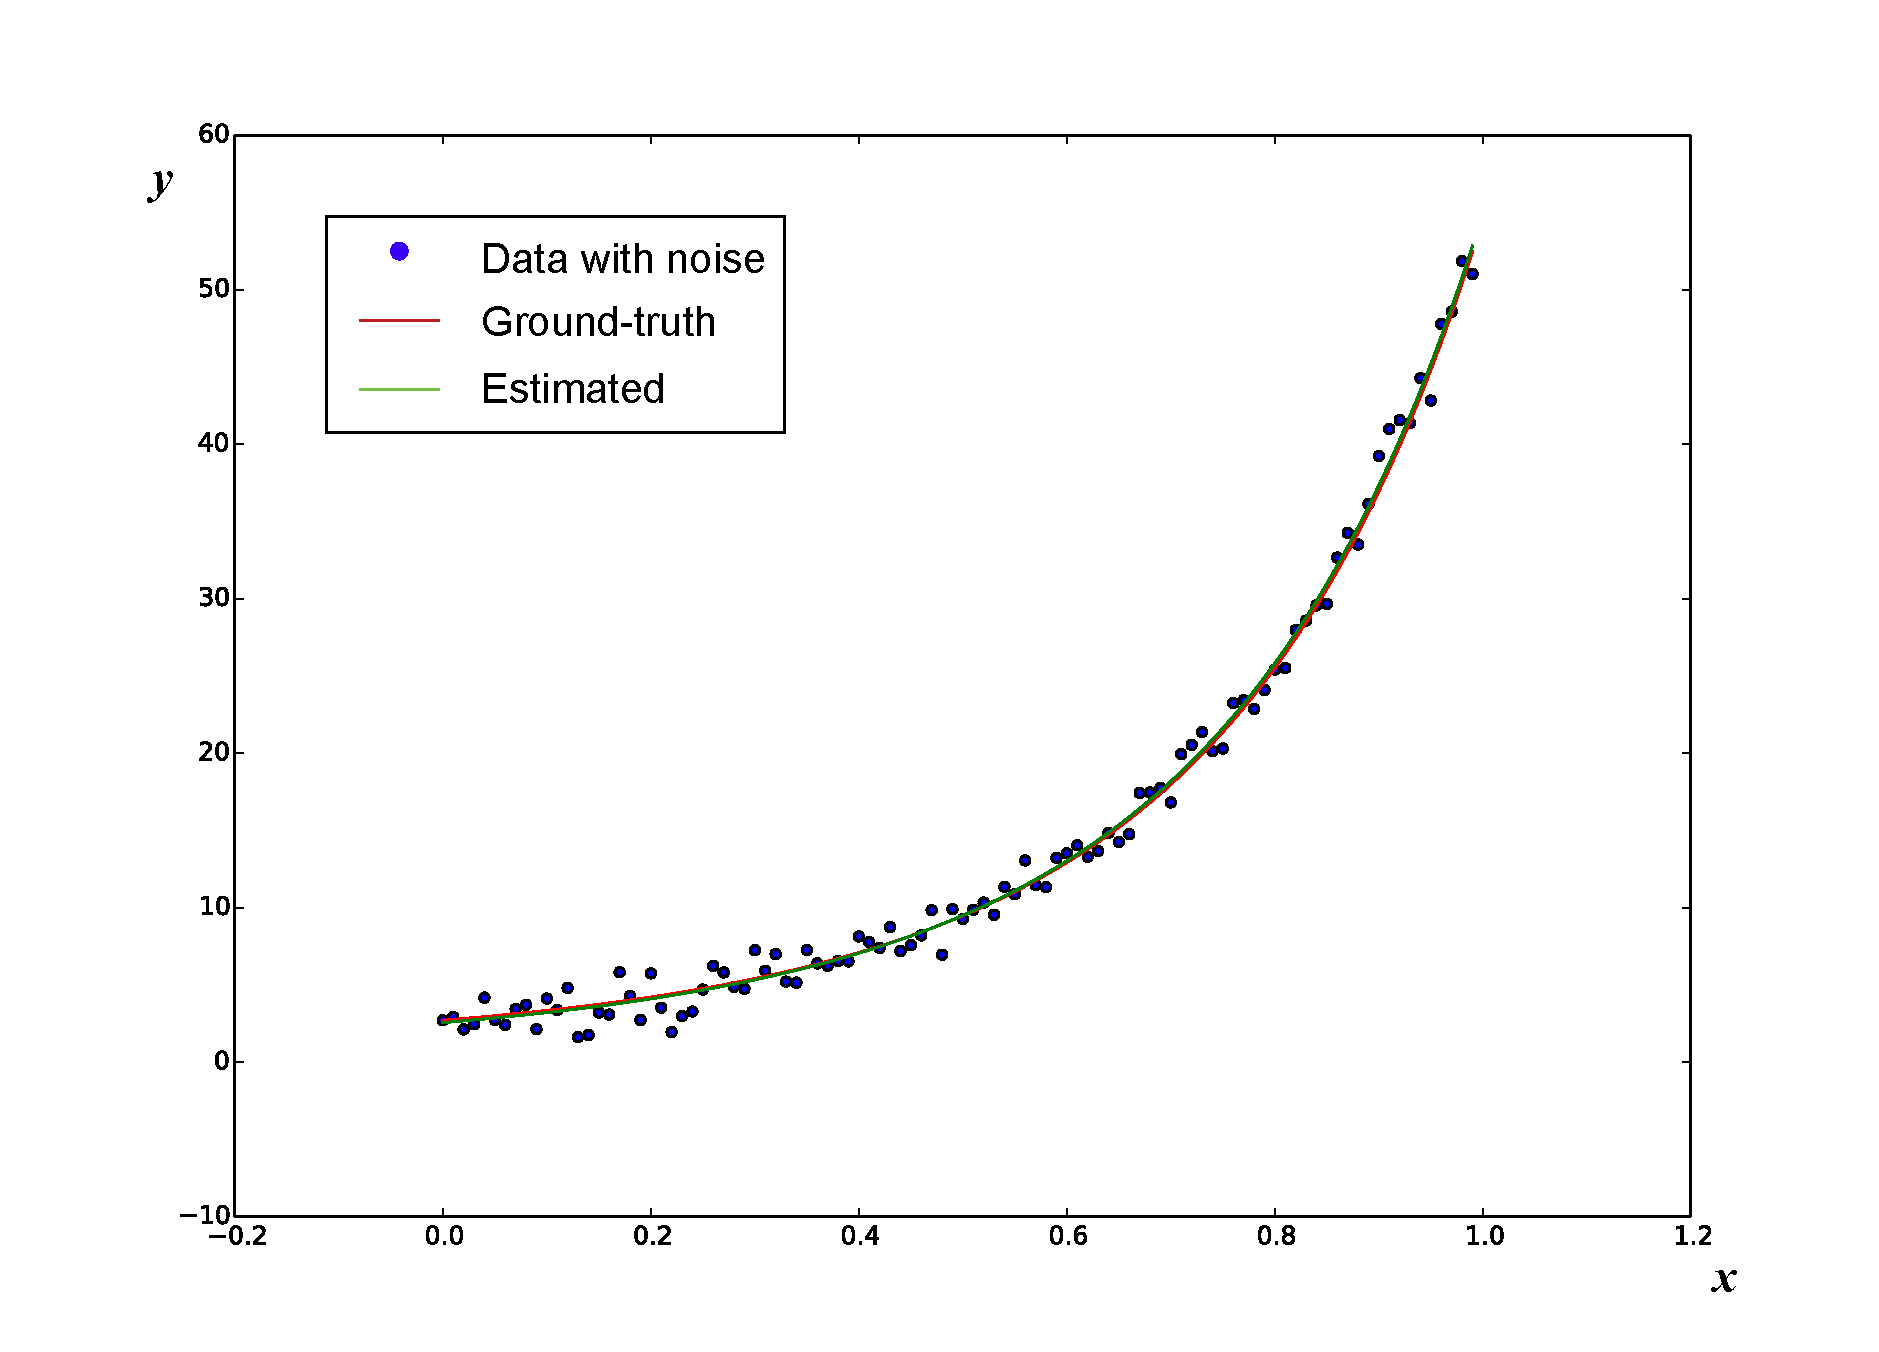
\includegraphics[width=0.8\textwidth]{optimization/ceresFitting.pdf}
    \caption{Estimated curve when the noise $\sigma=1$. }
    \label{fig:ceres-fitting}
\end{figure}

\subsection{Curve Fitting with Google Ceres}
In the next two sections we introduce two C++ optimization libraries: the Ceres library~\cite{Ceres} from Google and the \textit{g2o} library~\cite{Kummerle2011} based on graph optimization. Since in \textit{g2o}, we still need some knowledge about graph optimizations, we first go through the Ceres here, then introduce some graph optimization theories, and finally talk about \textit{g2o}. Since the optimization algorithms will still appear in the later chapters, please make sure you understand the meaning of the optimization algorithm and the content of the program.

\subsubsection{Introduction to Ceres}
Google Ceres is a widely used optimization library for least-square problems. In Ceres, as users, we only need to define the optimization problem to be solved according to specific steps and then hand it over to the solver for calculation. The most general form of the least-square problem solved by Ceres is as follows (kernel function least-squares with boundary):
\begin{equation}
    \begin{array}{ll}
        \min \limits_x \quad & \frac{1}{2}\sum\limits_i {{\rho _i}\left( {{{\left\| {{f_i}\left( {{x_{{i_1}}}, \cdots {x_{{i_n}}}} \right)} \right\|}^2}} \right)} \\
        \mathrm{s.t.} \quad & {l_j} \leqslant {x_j} \leqslant {u_j}.
    \end{array}
\end{equation}

In this question, $x_1, \cdots, x_n$ are optimized variables, also called parameter blocks, $f_i$ is called cost function, or residual blocks. $l_j$ and $u_j$ are the upper and lower limits of the $j$-th optimization variable. In the simplest case, we can set $l_j = -\infty, u_j=\infty$ (do not limit the boundary of the optimization variable). At this time, the objective function is composed of many square terms after the kernel function $\rho(\cdot)$ and then the sum \footnote{Kernel function is discussed in chapter~\ref{cpt:backend1}. }. Similarly, you can take $\rho$ as the identity function. The objective function is the sum of the squares of many terms.

In order to tell Ceres the definition of the problem, we need to do the following things:
\begin{enumerate}
    \item Defines each parameter block. The parameter block is usually a trivial vector, but it can also be defined as a particular structure such as quaternion and Lie algebra in SLAM. If it is a vector, we need to allocate a double array for each parameter block to store the variable's value.
    \item Then, define the calculation method of the residual block. The residual block is usually associated with several parameter blocks, performs some custom calculations on them, and then returns the residual value. After that, Ceres will sum the squares residuals, which is used as the overall objective function.
    \item In the residual blocks, we also need to define the Jacobian calculation method. In Ceres, we can use the ``automatic derivative'' function or manually specify the Jacobian calculation process. If you want to use automatic derivation, then the residual block must be written in a specific way: the residual calculation should be implemented as a bracketed operator with a template. We will illustrate this point through an example.
    \item Finally, add all the parameter blocks and residual blocks to Ceres's Problem object and call the Solve function to solve it. Before solving, we can pass some configuration information, such as the number of iterations, termination conditions, etc., or use the default configuration.
\end{enumerate}
Next, let's actually operate Ceres to solve the curve-fitting problem and understand the optimization process.

\subsubsection{Install Ceres}
In order to use Ceres, we first need to compile and install it. Ceres' GitHub address is \url{https://github.com/ceres-solver/ceres-solver}, and you can also directly use Ceres in our 3rdparty directory of the code repository so that you will use the same version as mine.

Like the libraries encountered before, Ceres is also a CMake project. Before compiling it, we need to install the dependencies first. You can install them with apt-get in Ubuntu, mainly some logging and testing tools used by Google:
\begin{lstlisting}[language=sh,caption=Terminal input: ]
sudo apt-get install liblapack-dev libsuitesparse-dev libcxsparse3 libgflags-dev libgoogle-glog-dev libgtest-dev 
\end{lstlisting}

Then, enter the Ceres library directory, use cmake to compile and install it. We have done this process many times, so I won't repeat it here. After the installation is complete, we can find the Ceres header file under /usr/local/include/ceres, and find the library file named libceres.a under /usr/local/lib/. With these files, we are able to include the Ceres headers and do the optimization calculations.

\subsubsection{Use Ceres for Curve Fitting}
The following code demonstrates how to use Ceres to solve the same problem.
\begin{lstlisting}[language=c++,caption=slambook/ch6/ceresCurveFitting.cpp]
#include <iostream>
#include <opencv2/core/core.hpp>
#include <ceres/ceres.h>
#include <chrono>

using namespace std;

// residual
struct CURVE_FITTING_COST {
    CURVE_FITTING_COST(double x, double y) : _x(x), _y(y) {}
    
    // implement operator () to compute the error
    template<typename T>
    bool operator()(
        const T *const abc, // the estimated variables, 3D vector
        T *residual) const {
        // y-exp(ax^2+bx+c)
        residual[0] = T(_y) - ceres::exp(abc[0] * T(_x) * T(_x) + abc[1] * T(_x) + abc[2]);
        return true;
    }
    
    const double _x, _y;    // x,y data 
};

int main(int argc, char **argv) {
    // same as before
    double ar = 1.0, br = 2.0, cr = 1.0;         // ground-truth values
    double ae = 2.0, be = -1.0, ce = 5.0;        // initial estimation
    int N = 100;                                 // num of data points
    double w_sigma = 1.0;                        // sigma of the noise
    double inv_sigma = 1.0 / w_sigma;
    cv::RNG rng;                                 // Random number generator 
    
    vector<double> x_data, y_data;      // the data
    for (int i = 0; i < N; i++) {
        double x = i / 100.0;
        x_data.push_back(x);
        y_data.push_back(exp(ar * x * x + br * x + cr) + rng.gaussian(w_sigma * w_sigma));
    }
    
    double abc[3] = {ae, be, ce};
    
    // construct the problem in ceres
    ceres::Problem problem;
    for (int i = 0; i < N; i++) {
        problem.AddResidualBlock(     // add i-th residual into the problem
            // use auto-diff, template params: redisual type, output dimension, input dimension
            // shoule be same as the struct written before
            new ceres::AutoDiffCostFunction<CURVE_FITTING_COST, 1, 3>(
                new CURVE_FITTING_COST(x_data[i], y_data[i])
            ),
            nullptr,            // kernel function, don't use here
            abc                 // estimated variables
        );
    }
    
    // set the solver options
    ceres::Solver::Options options;     // actually there're lots of params can be adjusted
    options.linear_solver_type = ceres::DENSE_NORMAL_CHOLESKY;  // use cholesky to solve the normal equation
    options.minimizer_progress_to_stdout = true;   // print to cout
    
    ceres::Solver::Summary summary;                
    chrono::steady_clock::time_point t1 = chrono::steady_clock::now();
    ceres::Solve(options, &problem, &summary);  // do optimization!
    chrono::steady_clock::time_point t2 = chrono::steady_clock::now();
    chrono::duration<double> time_used = chrono::duration_cast<chrono::duration<double>>(t2 - t1);
    cout << "solve time cost = " << time_used.count() << " seconds. " << endl;
    
    // get the outpus
    cout << summary.BriefReport() << endl;
    cout << "estimated a,b,c = ";
    for (auto a:abc) cout << a << " ";
    cout << endl;
    
    return 0;
}
\end{lstlisting}

The code is quite self-explained because we write a lot of comments here. As you can see, we used OpenCV's noise generator to generate 100 data with Gaussian noise and then used Ceres for fitting. The Ceres usage demonstrated here has the following steps:

\begin{enumerate}
    \item Defines the class of the residual block. The method is to write a class (or structure) and define the () operator with template parameters in the class to become a functor. \footnote{The functor is a C++ term. Such a class can be called as if it were a function because the operator () is overloaded.}  This definition allows Ceres to call the <double>() method for an instance of this class like a function. In fact, Ceres will pass the Jacobian matrix as a type parameter to this function to realize automatic derivation (auto-diff, which is one of the best features of Ceres).
    
    \item The double array abc[3] in the program is the parameter block. We construct a CURVE\_FITTING\_COST object for each data for the residual block and then call AddResidualBlock to add the error term to the objective function. Since the optimization requires gradients, we have several options: (1) Use Ceres's auto diff feature. (2) Use numeric diff \footnote{Automatic derivation is also implemented with numerical derivatives, but since it is a template operation, it runs faster. }; (3) Derive the analytical derivative form by yourself and provide it to Ceres. Because automatic derivation is the most convenient in coding, we use automatic derivation here.
    
    \item Automatic derivation requires specifying the dimensions of the error term and optimization variable. The error here is a scalar with a dimension of 1; the optimized three quantities are $a, b, c$ with 3. Therefore, the variable dimensions are set to 1, 3 in the template parameter of the auto-derivation class AutoDiffCostFunction.
    
    \item After setting the problem, call the Solve function to solve it. You can configure (very detailed) optimization options in Ceres. For example, you can choose to use line search or trust region, the number of iterations, step size, and so on. Readers can check the Ceres options to see what optimization methods are available. Of course, the default configuration can be used for a wide range of problems.
\end{enumerate}

Finally, let's see the experimental results by calling build/ceresCurveFitting: 
\begin{lstlisting}[caption=erminal output: ]
    iter      cost      cost_change  |gradient|   |step|    tr_ratio  tr_radius  ls_iter  iter_time  total_time
    0  1.597873e+06    0.00e+00    3.52e+06   0.00e+00   0.00e+00  1.00e+04        0    2.10e-05    7.92e-05
    1  1.884440e+05    1.41e+06    4.86e+05   9.88e-01   8.82e-01  1.81e+04        1    5.60e-05    1.05e-03
    2  1.784821e+04    1.71e+05    6.78e+04   9.89e-01   9.06e-01  3.87e+04        1    2.00e-05    1.09e-03
    3  1.099631e+03    1.67e+04    8.58e+03   1.10e+00   9.41e-01  1.16e+05        1    6.70e-05    1.16e-03
    4  8.784938e+01    1.01e+03    6.53e+02   1.51e+00   9.67e-01  3.48e+05        1    1.88e-05    1.19e-03
    5  5.141230e+01    3.64e+01    2.72e+01   1.13e+00   9.90e-01  1.05e+06        1    1.81e-05    1.22e-03
    6  5.096862e+01    4.44e-01    4.27e-01   1.89e-01   9.98e-01  3.14e+06        1    1.79e-05    1.25e-03
    7  5.096851e+01    1.10e-04    9.53e-04   2.84e-03   9.99e-01  9.41e+06        1    1.81e-05    1.28e-03
    solve time cost = 0.00130755 seconds. 
    Ceres Solver Report: Iterations: 8, Initial cost: 1.597873e+06, Final cost: 5.096851e+01, Termination: CONVERGENCE
    estimated a,b,c = 0.890908 2.1719 0.943628 
\end{lstlisting}

The final optimized value is basically the same as our experimental result in the previous section, but Ceres is relatively slow in running speed. Ceres used about 1.3 milliseconds on my machine, which is about six times slower than the handwritten Gauss-Newton method.

I hope readers have a general understanding of how to use Ceres through this simple example. Its advantage is that it provides an automatic derivation tool, making it unnecessary to calculate the troublesome Jacobian matrix. Ceres's automatic derivation is realized through template elements, and the automatic derivation can be completed at compile-time, but it is still a numerical derivative. Most of the time in this book, I will still introduce the Jacobian matrix calculation because it helps understand the problem. Besides, Ceres' optimization process configuration is also very rich, making it suitable for a wide range of least-squares optimization problems, including various problems other than SLAM.

\subsection{Curve Fitting with \textit{g2o}}
The second practice part of this lecture is about another optimization library (widely used mainly in the SLAM field): \textit{g2o} (general graphic optimization, g$^2$o). It is a library based on \textit{graphic optimization}. Graph optimization is a theory that combines nonlinear optimization with graph theory, so before using it, let's spend a little space to introduce graph optimization theory.

\subsubsection{Introduction to Graph Optimization Theory}
We have introduced the solution of nonlinear least-squares. The least-square problem in SLAM is normally composed of the sum of many small error terms. However, if we only treat them as variables and residuals, it would be hard to tell the \textit{relationship} between them. For example, how many error terms are related to a certain optimization variable $x_j$? If we adjust some variables, does the overall cost function change or keep the same? Furthermore, we hope to visually see what optimization problem \textit{looks like}. Therefore, graph optimization is involved.

Graph optimization is a way to express the optimization problem as a graph.  A graph consists of a number of vertices and edges connecting these vertices. A  vertex is used to represent an optimization variable, and an edge is used to represent an error term. Therefore, for any of the above-mentioned nonlinear least-squares problems, we can construct a corresponding graph. We can simply call it a graph or use the probability graph definition, call it a Bayesian graph or a factor graph. Sometimes it is also called a hypergraph because an edge can be connected to more than two variables, e.g., where an error term is related to more than two variables. 

\autoref{fig:graph-optimization}~ is a simple graph optimization example. We use triangles to represent the camera poses and circles to represent landmark points, which constitute the vertices. At the same time, the solid line represents the camera's motion model, and the dashed line represents the observation model, which forms the edges of the graph optimization. At this point, although the mathematical form of the entire problem is still like \eqref{eq:least-square}, now we can intuitively see the structure of the problem. If you want, you can also make improvements like removing isolated vertices or preferentially optimizing vertices with more edges (or, in graph theory terms, greater degrees). But the most basic idea is just to use a graph model to express a nonlinear least-squares optimization problem. And we can use some properties of the graph model to do better optimization.

\begin{figure}[!ht]
    \centering
    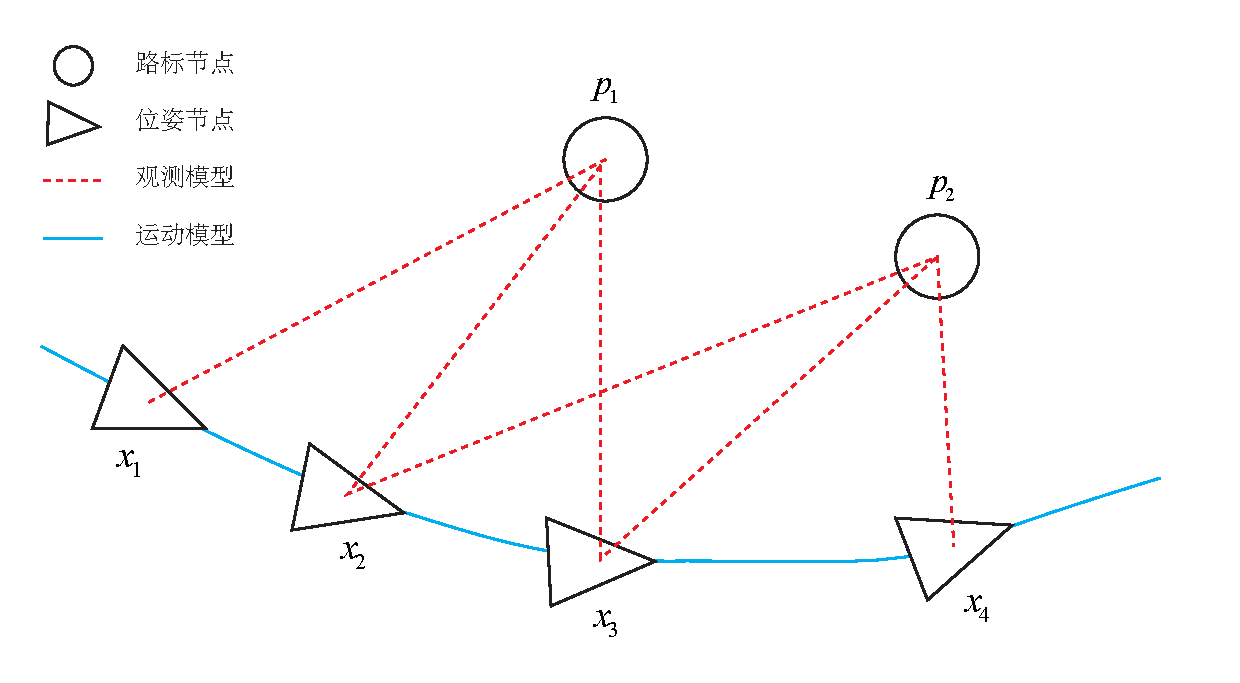
\includegraphics[width=1.0\textwidth]{optimization/graphOptimization.pdf}
    \caption{An example of the graph optimization.}
    \label{fig:graph-optimization}
\end{figure}

The \textit{g2o} is a \textit{general} graph optimization library. ``General'' means that you can solve any least-squares problem that can be expressed as graph optimization, obviously including the curve-fitting problem discussed above. Let us demonstrate how to do that.

\subsubsection{Compilation and Installation of \textit{g2o}}
Just like the Ceres section, we should first compile and install the \textit{g2o} library. Readers should have experienced this process many times, and they are basically the same. Regarding \textit{g2o}, readers can download it from GitHub: \url{https://github.com/RainerKuemmerle/g2o}, or obtain it from the third-party code library provided in this book. Since \textit{g2o} is still being updated, I suggest using \textit{g2o} under 3rdparty to ensure that the version is the same as mine.

\textit{g2o} is also a cmake project. Let's install its dependencies first (some dependencies overlap with Ceres):
\begin{lstlisting}[language=sh,caption=Terminal input:]
    sudo apt-get install qt5-qmake qt5-default libqglviewer-dev-qt5 libsuitesparse-dev libcxsparse3 libcholmod3
\end{lstlisting}

Then, compile and install \textit{g2o} according to the cmake method. The description of the process is omitted here. After the installation is complete, the header files of \textit{g2o} will be located under ``/usr/local/g2o'', and the library files will be located under /usr/local/lib/. We reconsider the curve fitting experiment in the Ceres routine and do that experiment again in \textit{g2o}.

\subsubsection{Curve Fitting with \textit{g2o}}
In order to use \textit{g2o}, the curve fitting problem must first be constructed into graph optimization. In this process, just remember that nodes are the optimization variables, and edges are the error terms. The graph optimization problem of curve fitting can be drawn in the form of \autoref{fig:graph-fitting}~.

\begin{figure}[!ht]
    \centering
    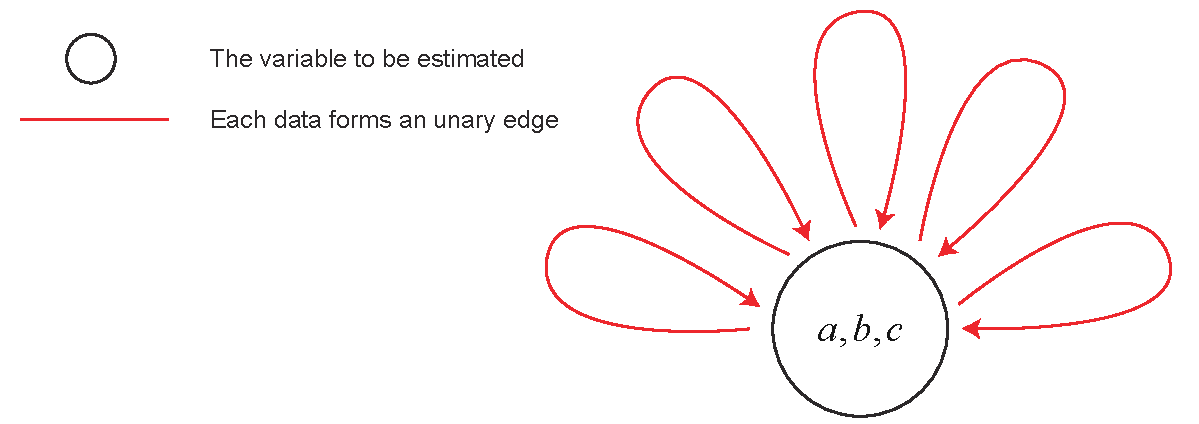
\includegraphics[width=.9\textwidth]{optimization/graphFitting.pdf}
    \caption{Graph model of the curve fitting problem. }
    \label{fig:graph-fitting}
\end{figure}

The entire problem has only one vertex: the parameters $a, b, c$ of the curve model. Each noisy data point constitutes an error term, which is the edge of the graph optimization. But the edges here are not the same as we usually think. They are unary edges, which means that the edges connect only one vertex. Because the entire graph has only one vertex. So in \autoref{fig:graph-fitting}~, we can only draw it as if it is connected to itself. An edge in graph optimization can connect one, two, or more vertices, reflecting how many optimization variables each error is related to. In a slightly mysterious way, we call it a hyperedge. The whole graph is called hypergraph \footnote{I personally would better call it just as a graph to avoid being mysterious. }.

After clarifying the graph model, the next step is to build the model in \textit{g2o} for optimization. As a user of \textit{g2o}, what we need to do mainly includes the following steps:
\begin{enumerate}
    \item Define the type of vertices and edges.
    \item Build the graph.
    \item Select the optimization algorithm.
    \item Call \textit{g2o} to optimize and get the result.
\end{enumerate}

This part is very similar to Ceres. Of course there will be some differences in coding. Let's demonstrate the program.
\begin{lstlisting}[language=c++,caption=slambook/ch6/g2oCurveFitting.cpp]
#include <iostream>
#include <g2o/core/g2o_core_api.h>
#include <g2o/core/base_vertex.h>
#include <g2o/core/base_unary_edge.h>
#include <g2o/core/block_solver.h>
#include <g2o/core/optimization_algorithm_levenberg.h>
#include <g2o/core/optimization_algorithm_gauss_newton.h>
#include <g2o/core/optimization_algorithm_dogleg.h>
#include <g2o/solvers/dense/linear_solver_dense.h>
#include <Eigen/Core>
#include <opencv2/core/core.hpp>
#include <cmath>
#include <chrono>

using namespace std;

// vertex: 3d vector 
class CurveFittingVertex : public g2o::BaseVertex<3, Eigen::Vector3d> {
public:
    EIGEN_MAKE_ALIGNED_OPERATOR_NEW
    
    // override the reset function
    virtual void setToOriginImpl() override {
        _estimate << 0, 0, 0;
    }
    
    // override the plus operator, just plain vector addition
    virtual void oplusImpl(const double *update) override {
        _estimate += Eigen::Vector3d(update);
    }
    
    // the dummy read/write function
    virtual bool read(istream &in) {}
    virtual bool write(ostream &out) const {}
};

// edge: 1D error term, connected to exactly one vertex
class CurveFittingEdge : public g2o::BaseUnaryEdge<1, double, CurveFittingVertex> {
public:
    EIGEN_MAKE_ALIGNED_OPERATOR_NEW
    
    CurveFittingEdge(double x) : BaseUnaryEdge(), _x(x) {}
    
    // define the error term computation
    virtual void computeError() override {
        const CurveFittingVertex *v = static_cast<const CurveFittingVertex *> (_vertices[0]);
        const Eigen::Vector3d abc = v->estimate();
        _error(0, 0) = _measurement - std::exp(abc(0, 0) * _x * _x + abc(1, 0) * _x + abc(2, 0));
    }
    
    // the jacobian
    virtual void linearizeOplus() override {
        const CurveFittingVertex *v = static_cast<const CurveFittingVertex *> (_vertices[0]);
        const Eigen::Vector3d abc = v->estimate();
        double y = exp(abc[0] * _x * _x + abc[1] * _x + abc[2]);
        _jacobianOplusXi[0] = -_x * _x * y;
        _jacobianOplusXi[1] = -_x * y;
        _jacobianOplusXi[2] = -y;
    }
    
    virtual bool read(istream &in) {}
    virtual bool write(ostream &out) const {}
public:
    double _x;  // x data, note y is given in _measurement
};

int main(int argc, char **argv) {
    // ... we omit the data sampling code, same as before
    typedef g2o::BlockSolver<g2o::BlockSolverTraits<3, 1>> BlockSolverType;  // bolck solver 
    typedef g2o::LinearSolverDense<BlockSolverType::PoseMatrixType> LinearSolverType; // linear solver
    
    // choose the optimizatoin method from GN, LM, DogLeg 
    auto solver = new g2o::OptimizationAlgorithmGaussNewton(
        g2o::make_unique<BlockSolverType>(g2o::make_unique<LinearSolverType>()));
    g2o::SparseOptimizer optimizer;    // graph optimizer
    optimizer.setAlgorithm(solver);    // set the algorithm
    optimizer.setVerbose(true);        // print the results
    
    // add vertex
    CurveFittingVertex *v = new CurveFittingVertex();
    v->setEstimate(Eigen::Vector3d(ae, be, ce));
    v->setId(0);
    optimizer.addVertex(v);
    
    // add edges
    for (int i = 0; i < N; i++) {
        CurveFittingEdge *edge = new CurveFittingEdge(x_data[i]);
        edge->setId(i);
        edge->setVertex(0, v);                // connect to the vertex
        edge->setMeasurement(y_data[i]);      // measurement
        edge->setInformation(Eigen::Matrix<double, 1, 1>::Identity() * 1 / (w_sigma * w_sigma)); // set the information matrix
        optimizer.addEdge(edge);
    }
    
    // carry out the optimization
    cout << "start optimization" << endl;
    chrono::steady_clock::time_point t1 = chrono::steady_clock::now();
    optimizer.initializeOptimization();
    optimizer.optimize(10);
    chrono::steady_clock::time_point t2 = chrono::steady_clock::now();
    chrono::duration<double> time_used = chrono::duration_cast<chrono::duration<double>>(t2 - t1);
    cout << "solve time cost = " << time_used.count() << " seconds. " << endl;
    
    // print the results
    Eigen::Vector3d abc_estimate = v->estimate();
    cout << "estimated model: " << abc_estimate.transpose() << endl;
    
    return 0;
}
\end{lstlisting}

In this program, we derive graph optimization vertices and edges for curve fitting from \textit{g2o} built-in classes: CurveFittingVertex and CurveFittingEdge, which essentially expands the use of \textit{g2o}. These two classes are derived from BaseVertex and BaseUnaryEdge, respectively. In the derived classes, we have rewritten some important virtual functions:
\begin{enumerate}
    \item Vertex update function: \textit{oplusImpl}. We know that the most important thing in the optimization process is the calculation of incremental $\Delta \mathbf{x}$, and this function deals with $\mathbf{x}_{k+1} = \mathbf{x}_k + \Delta \mathbf{x}$ process.

    Readers may think this is not something worth mentioning because it is just simple addition. Why doesn't \textit{g2o} help us complete it? In the curve fitting process, since the optimization variables (curve parameters) are located in the plain vector space, this update calculation is indeed nothing but just simple addition. However, when the optimization variable is not in the vector space, for example, for $\mathbf{x}$ is the camera pose, it does not necessarily have an addition operation. At this time, it is necessary to redefine the behavior of how the increment is added to the existing estimate. According to the explanation in lecture~\ref{cpt:4}, we may use the left-multiplication update or the right-multiplication update instead of direct addition.

    \item Vertex reset function: \textit{setToOriginImpl}. This is trivial, and we just set the estimate to zero.

    \item The error calculation function: computeError. According to the curve model, this function needs to take out the current estimated value of the vertex connected by the edge and compare it with its observed value. This is consistent with the error model in the least-squares problem.
    
    \item The Jacobian calculation function: \textit{linearizeOplus}. In this function, we calculate the Jacobian of each edge relative to the vertex.

    \item Save and read functions: read, write. Since we do not want to perform read/write operations, leave it blank.
\end{enumerate}

After defining the vertices and edges, we declare a graph model in the main function, then add vertices and edges to the graph model according to the generated noise data, and finally call the optimization function for optimization. \textit{g2o} will give the optimized result:
\begin{lstlisting}[language=sh,caption=Terminal output:]
start optimization
iteration= 0	 chi2= 376785.128234	 time= 3.3299e-05	 cumTime= 3.3299e-05	 edges= 100	 schur= 0
iteration= 1	 chi2= 35673.566018	 time= 1.3789e-05	 cumTime= 4.7088e-05	 edges= 100	 schur= 0
iteration= 2	 chi2= 2195.012304	 time= 1.2323e-05	 cumTime= 5.9411e-05	 edges= 100	 schur= 0
iteration= 3	 chi2= 174.853126	 time= 1.3302e-05	 cumTime= 7.2713e-05	 edges= 100	 schur= 0
iteration= 4	 chi2= 102.779695	 time= 1.2424e-05	 cumTime= 8.5137e-05	 edges= 100	 schur= 0
iteration= 5	 chi2= 101.937194	 time= 1.2523e-05	 cumTime= 9.766e-05	 edges= 100	 schur= 0
iteration= 6	 chi2= 101.937020	 time= 1.2268e-05	 cumTime= 0.000109928	 edges= 100	 schur= 0
iteration= 7	 chi2= 101.937020	 time= 1.2612e-05	 cumTime= 0.00012254	 edges= 100	 schur= 0
iteration= 8	 chi2= 101.937020	 time= 1.2159e-05	 cumTime= 0.000134699	 edges= 100	 schur= 0
iteration= 9	 chi2= 101.937020	 time= 1.2688e-05	 cumTime= 0.000147387	 edges= 100	 schur= 0
solve time cost = 0.000919301 seconds. 
estimated model: 0.890912   2.1719 0.943629
\end{lstlisting}

We use the Gauss-Newton method for gradient descent, and after 9 iterations, the optimization result is obtained, which is almost the same as the Ceres and handwritten Gauss-Newton method. From the running speed perspective, our experimental conclusion is that handwriting is faster than \textit{g2o}, and \textit{g2o} is faster than Ceres. This is a generally intuitive experience that versatility and efficiency are often contradictory. However, in this experiment, Ceres uses automatic derivation, and the solver configuration is not completely consistent with Gauss-Newton, so it seems slower.

\section{Summary}
This section introduces a nonlinear optimization problem often encountered in SLAM: the least-squares problem consisting of the sum of squares of many error terms. We introduced its definition and solution and discussed two main gradient descent methods: the Gauss-Newton method and the Levenberg-Marquardt method. In the practice part, two optimization libraries of the handwritten Gauss-Newton method, Ceres and \textit{g2o}, were used to solve the same curve-fitting problem and found that they gave similar results.

Since the bundle adjustment has not been discussed in detail, we have chosen a simple but representative example of curve fitting in the practice part to demonstrate the general nonlinear least-squares solution method. In particular, if you use \textit{g2o} to fit a curve, you must first convert the problem to graph optimization and define new vertices and edges. This approach is somewhat roundabout—the main purpose of \textit{g2o} is not here. In contrast, Ceres' usage is much more natural because it is designed to be a general optimization library. However, the SLAM problem is about solving an optimization problem with many camera poses and many spatial points. In particular, when the camera pose is represented by Lie algebra, calculating the derivative of the camera pose in the error term will be worthy of detailed discussion. We will find in the follow-up content that \textit{g2o} provides a large number of ready-to-use vertices and edges, which is very convenient for the camera pose estimation problem. In Ceres, we have to implement each cost function by ourselves, which has some inconveniences.

In the two programs of the practical part, we did not calculate the derivative of the curve model with respect to the three parameters but used the numerical derivative of the optimization library, which made the theory and code simpler. The Ceres library provides automatic derivation based on template elements and numerical derivation at runtime, while \textit{g2o} only provides a numerical derivation method. However, for most problems, if you can derive the analytical form of the Jacobian matrix and tell the optimization library, you can avoid many problems in numerical derivation.

Finally, I hope readers can adapt to Ceres and \textit{g2o}'s extensive use of template programming. It may seem scary at first (especially the parenthesis operator for Ceres to set the residual block and the code for the \textit{g2o} initialization part). But once you are familiar with it, you will feel that this method is natural and easy to extend. We will continue to discuss issues such as sparsity, kernel functions, and pose graphs in the SLAM backend lecture.

\section*{Exercises}
\begin{enumerate}
    \item Prove that in the linear equation $\mathbf{A} \mathbf{x} = \mathbf{b}$, when the coefficient matrix $\mathbf{A}$ is over-determined, the least-square solution is $\mathbf{x} = (\mathbf{A}^T\mathbf{A})^{-1}\mathbf{A}^T \mathbf{b}$.
    \item Investigate the advantages and disadvantages of the steepest descent method, Newton method, Gauss-Newton method, and Levenberg-Marquardt method. In addition to the Ceres library and \textit{g2o} library we cited, are there any commonly used optimization libraries? (You may find some libraries on MATLAB.)
    \item Why does the coefficient matrix of the Gauss-Newton method's incremental equation may not be positive definite? What is the geometric meaning of indefinite? Why is the solution unstable in this case?
    \item What is DogLeg? What are the similarities and differences between it and the Gauss-Newton method and the Levenberg-Marquardt method? Please search for relevant materials \footnote{\url{http://www.numerical.rl.ac.uk/people/nimg/course/lectures/raphael/lectures/lec7slides.pdf}. }.
    \item Read Ceres' tutorials (\url{http://ceres-solver.org/tutorial.html}) to better understand its usage.
    \item Read the documentation that comes with \textit{g2o}, can you understand it? If you still can't fully understand it, please come back after lectures~\ref{cpt:backend1} and~\ref{cpt:backend2}.
    \item[\optional] Please change the curve model in the curve fitting experiment, and use Ceres and \textit{g2o} to optimize it. For example, write an example with more parameters and more complex models.
\end{enumerate}

\part{SLAM Technologies}
% !Mode:: "TeX:UTF-8"
\chapter{视觉里程计1}
\label{cpt:7}
\thispagestyle{empty}

\begin{mdframed}  
	\textbf{主要目标}
	\begin{enumerate}[labelindent=0em,leftmargin=1.5em]
		\item 理解图像特征点的意义, 并掌握在单幅图像中提取出特征点及多幅图像中匹配特征点的方法。
		\item 理解对极几何的原理,利用对极几何的约束,恢复出图像之间的摄像机的三维运动。
		\item 理解PNP问题,以及利用已知三维结构与图像的对应关系求解摄像机的三维运动。
		\item 理解ICP问题,以及利用点云的匹配关系求解摄像机的三维运动。
		\item 理解如何通过三角化获得二维图像上对应点的三维结构。
	\end{enumerate}
\end{mdframed}

本书前面介绍了运动方程和观测方程的具体形式,并讲解了以非线性优化为主的求解方法。从本讲开始,我们结束基础知识的铺垫而步入正题:按照第2讲的顺序,分别介绍视觉里程计、优化后端、回环检测和地图构建4个模块。本讲和下一讲主要介绍两类视觉里程计里常用的方法:特征点法和光流法。本讲中,我们将介绍什么是特征点、如何提取和匹配特征点,以及如何根据配对的特征点估计相机运动。

\newpage
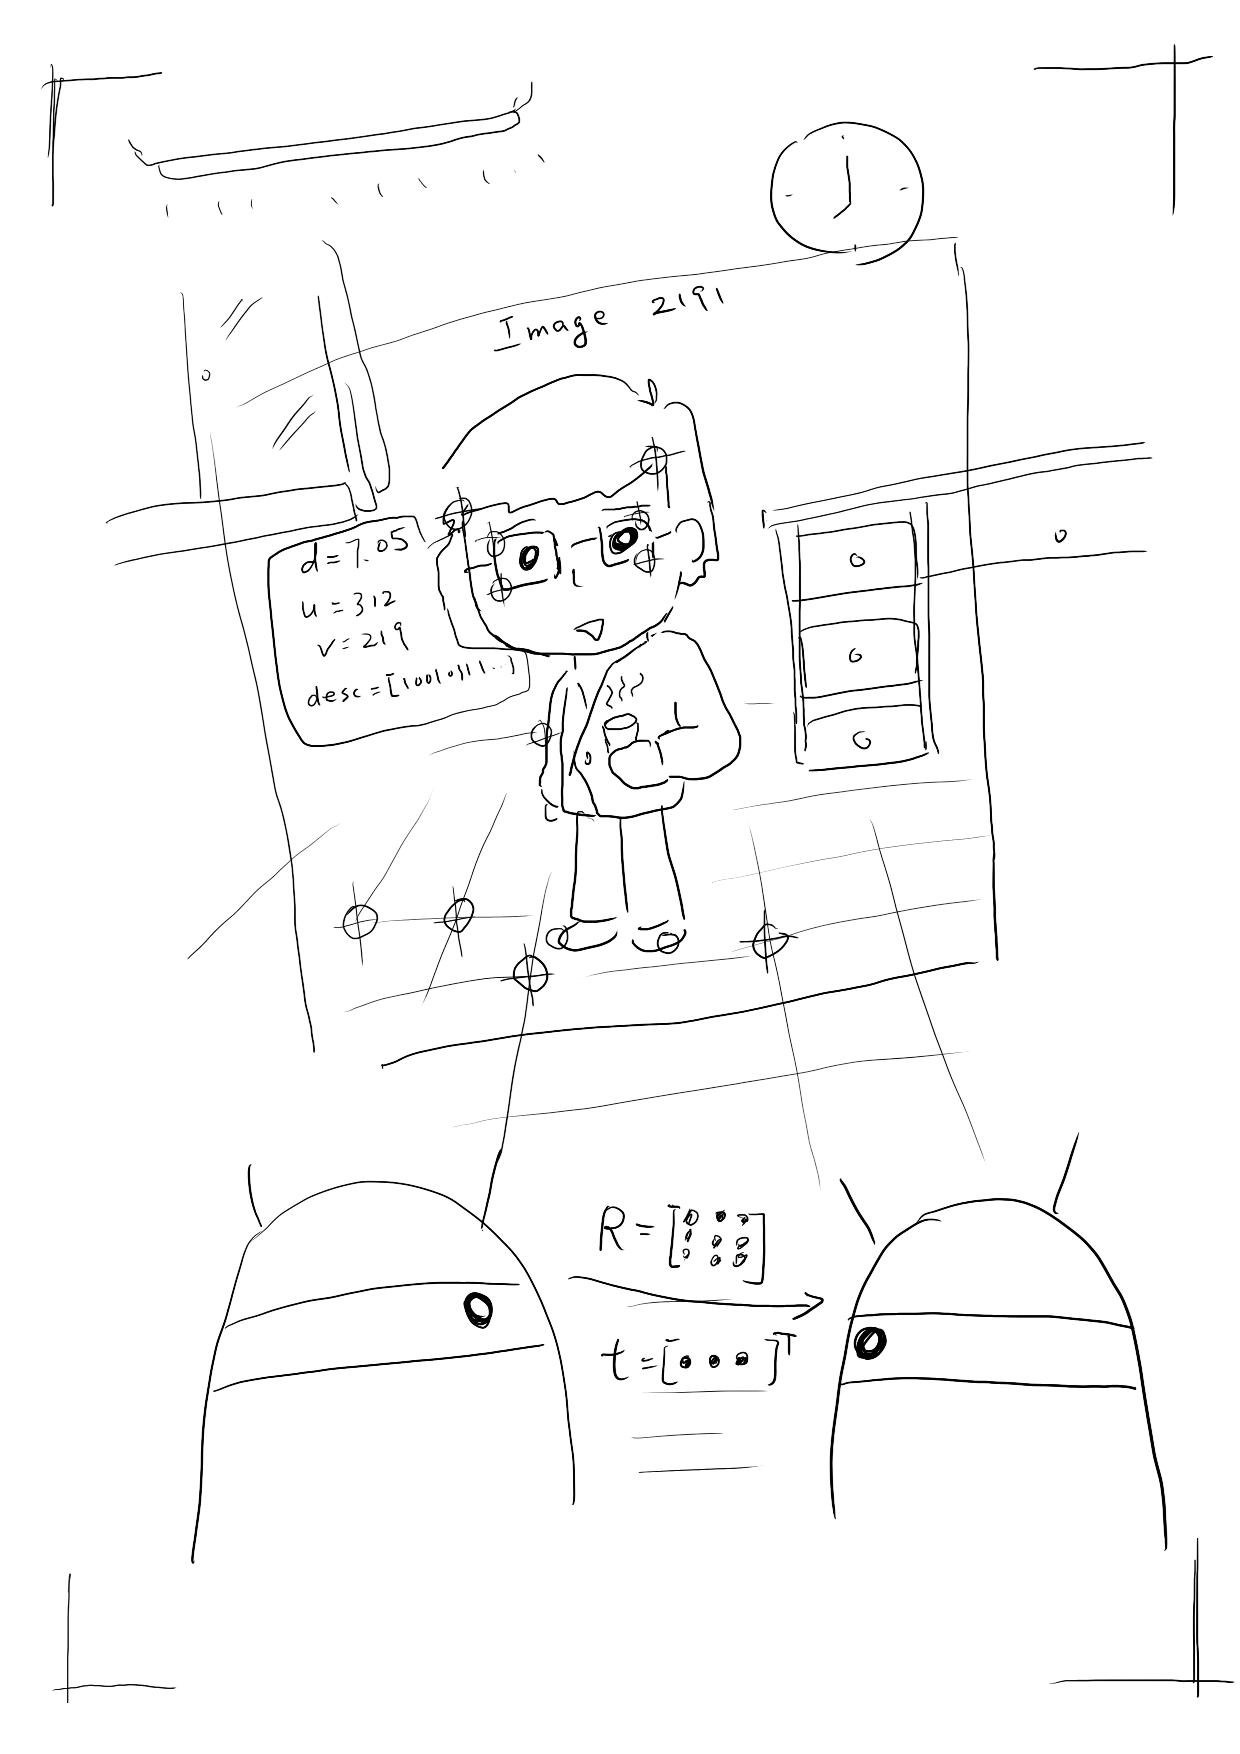
\includepdf{resources/other/ch7.pdf}

\newpage

\section{特征点法}
在第二讲中,我们说,一个SLAM系统分为前端和后端,其中前端也称为视觉里程计(VO)。VO根据相邻图像的信息估计出粗略的相机运动,给后端提供较好的初始值。VO的算法主要分为两个大类:\textbf{特征点法}和\textbf{直接法}。基于特征点法的前端,长久以来(直到现在)被认为是视觉里程计的主流方法。它具有稳定,对光照、动态物体不敏感的优势,是目前比较成熟的解决方案。在本讲中,我们将从特征点法入手,学习如何提取、匹配图像特征点,然后估计两帧之间的相机运动和场景结构,从而实现一个两帧间视觉里程计。这类算法有时也称为两视图几何(Two-view geometry)。

\subsection{特征点}
VO的核心问题是\textbf{如何根据图像来估计相机运动}。然而,图像本身是一个由亮度和色彩组成的矩阵,如果直接从矩阵层面考虑运动估计,将会非常困难。所以,比较方便的做法是:首先,从图像中选取比较\textbf{有代表性}的\textbf{点}。这些点在相机视角发生少量变化后会保持不变,于是我们能在各个图像中找到相同的点。然后,在这些点的基础上,讨论相机位姿估计问题,以及这些点的定位问题。在经典SLAM模型中,我们称这些点为\textbf{路标}(Landmark)。而在视觉SLAM中,路标则是指图像特征(Feature)。

根据维基百科的定义,图像特征是一组与计算任务相关的信息,计算任务取决于具体的应用\textsuperscript{\cite{wiki:featurecv}}。简而言之,\textbf{特征是图像信息的另一种数字表达形式}。一组好的特征对于在指定任务上的最终表现至关重要,所以多年来研究者们花费了大量的精力对特征进行研究。数字图像在计算机中以灰度值矩阵的方式存储,所以最简单的,单个图像像素也是一种“特征”。但是,在视觉里程计中,我们希望\textbf{特征点在相机运动之后保持稳定},而灰度值受光照、形变、物体材质的影响严重,在不同图像间变化非常大,不够稳定。理想的情况是,当场景和相机视角发生少量改变时,算法还能从图像中判断哪些地方是同一个点。所以,仅凭灰度值是不够的,我们需要对图像提取特征点。

特征点是图像里一些\textbf{特别的地方}。以\autoref{fig:corner-feature}~为例。我们可以把图像中的角点、边缘和区块都当成图像中有代表性的地方。不过,我们更容易精确地指出,某两幅图像中出现了同一个角点;同一个边缘则稍微困难一些,因为沿着该边缘前进,图像局部是相似的;同一个区块则是最困难的。我们发现,图像中的角点、边缘相比于像素区块而言更加“特别”,在不同图像之间的辨识度更强。所以,一种直观的提取特征的方式就是在不同图像间辨认角点,确定它们的对应关系。在这种做法中,角点就是所谓的特征。角点的提取算法有很多,例如Harris角点\textsuperscript{\cite{Harris1988}}、FAST角点\textsuperscript{\cite{Rosten2006}}、GFTT角点\textsuperscript{\cite{Shi1994}},等等。它们大部分是2000年以前提出的算法。

然而,在大多数应用中,单纯的角点依然不能满足我们的很多需求。例如,从远处看上去是角点的地方,当相机走近之后,可能就不显示为角点了。或者,当旋转相机时,角点的外观会发生变化,我们也就不容易辨认出那是同一个角点。为此,计算机视觉领域的研究者们在长年的研究中设计了许多更加稳定的局部图像特征,如著名的SIFT\textsuperscript{\cite{Lowe2004}}、SURF\textsuperscript{\cite{Bay2006}}、ORB\textsuperscript{\cite{Rublee2011}},等等。相比于朴素的角点,这些人工设计的特征点能够拥有如下的性质:

\begin{enumerate}
\item \emph{可重复性}(Repeatability):相同的特征可以在不同的图像中找到。
\item \emph{可区别性}(Distinctiveness):不同的特征有不同的表达。
\item \emph{高效率}(Efficiency):同一图像中,特征点的数量应远小于像素的数量。
\item \emph{本地性}(Locality):特征仅与一小片图像区域相关。
\end{enumerate}

\begin{figure}[!ht]
    \centering
    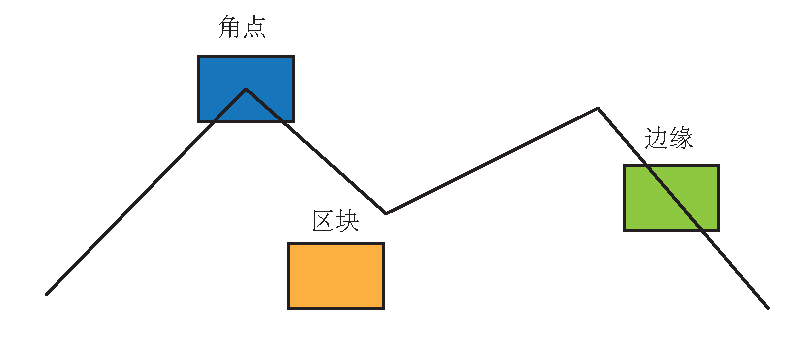
\includegraphics[width=0.8\linewidth]{vo1/corner-flat-line}\\
    \caption{可以作为图像特征的部分:角点、边缘、区块。}
    \label{fig:corner-feature}
\end{figure}

特征点由\textbf{关键点}(Key-point)和\textbf{描述子}(Descriptor)两部分组成。比如,当我们说“在一张图像中计算SIFT特征点”,是指“提取SIFT关键点,并计算SIFT描述子”两件事情。关键点是指该特征点在图像里的位置,有些特征点还具有朝向、大小等信息。描述子通常是一个向量,按照某种人为设计的方式,描述了该关键点周围像素的信息。描述子是按照“\textbf{外观相似的特征应该有相似的描述子}”的原则设计的。因此,只要两个特征点的描述子在向量空间上的距离相近,就可以认为它们是同样的特征点。

历史上,研究者们提出过许多图像特征。它们有些很精确,在相机的运动和光照变化下仍具有相似的表达,但相应地需要较大的计算量。其中,SIFT(尺度不变特征变换,Scale-Invariant Feature Transform)当属最为经典的一种。它充分考虑了在图像变换过程中出现的光照、尺度、旋转等变化,但随之而来的是极大的计算量。由于整个SLAM过程中图像特征的提取与匹配仅仅是诸多环节中的一个,到目前(2016年)为止,普通PC的CPU还无法实时地计算SIFT特征,进行定位与建图\footnote{这里是指30Hz的实时速度。}。所以在SLAM中我们甚少使用这种“奢侈”的图像特征。

另一些特征,则考虑适当降低精度和鲁棒性,以提升计算的速度。例如,FAST关键点属于计算特别快的一种特征点(注意这里“关键点”的表述,说明它没有描述子),而ORB(Oriented FAST and Rotated BRIEF)特征则是目前看来非常具有代表性的实时图像特征。它改进了FAST检测子\textsuperscript{\cite{Rosten2006}}不具有方向性的问题,并采用速度极快的二进制描述子BRIEF\textsuperscript{\cite{calonder2010brief}},使整个图像特征提取的环节大大加速。根据作者在论文中所述测试,在同一幅图像中同时提取约1000个特征点的情况下,ORB约要花费15.3ms,SURF约花费217.3ms,SIFT约花费5228.7ms。由此可以看出,ORB在保持了特征子具有旋转、尺度不变性的同时,速度方面提升明显,对于实时性要求很高的SLAM来说是一个很好的选择。

大部分特征提取都具有较好的并行性,可以通过GPU等设备来加速计算。经过GPU加速后的SIFT,就可以满足实时计算要求。但是,引入GPU将带来整个SLAM成本的提升。由此带来的性能提升是否足以抵去付出的计算成本,需要系统的设计人员仔细考量。

显然,计算机视觉领域存在大量的特征点种类,我们不可能在书中一一介绍。在目前的SLAM方案中,ORB是质量与性能之间较好的折中,因此,我们以ORB为代表介绍提取特征的整个过程。如果读者对特征提取和匹配算法感兴趣,我们建议阅读这方面的相关书籍\cite{Nixon2012}。

\subsection{ORB特征}

ORB特征亦由\textbf{关键点}和\textbf{描述子}两部分组成。它的关键点称为“Oriented FAST”,是一种改进的FAST角点,关于什么是FAST角点我们将在下文介绍。它的描述子称为BRIEF(Binary Robust Independent Elementary Feature)。因此,提取ORB特征分为如下两个步骤:
\begin{enumerate}
\item FAST角点提取:找出图像中的“角点”。相较于原版的FAST,ORB中计算了特征点的主方向,为后续的BRIEF描述子增加了旋转不变特性。
\item BRIEF描述子:对前一步提取出特征点的周围图像区域进行描述。ORB对BRIEF进行了一些改进,主要是指在BRIEF中使用了先前计算的方向信息。
\end{enumerate}

下面分别介绍FAST和BRIEF。
\subsubsection{FAST关键点}

FAST是一种角点,主要检测局部像素灰度变化明显的地方,以速度快著称。它的思想是:如果一个像素与邻域的像素差别较大(过亮或过暗),那么它更可能是角点。相比于其他角点检测算法,FAST只需比较像素亮度的大小,十分快捷。它的检测过程如下(见\autoref{fig:fastcorner}~):

\begin{enumerate}
\item 在图像中选取像素$p$,假设它的亮度为$I_{p}$。
\item 设置一个阈值$T$(比如,$I_{p}$的20\%)。
\item 以像素$p$为中心,选取半径为3的圆上的16个像素点。
\item 假如选取的圆上有连续的$N$个点的亮度大于$I_{p}+T$或小于$I_{p}-T$,那么像素$p$可以被认为是特征点($N$通常取12,即为FAST-12。其他常用的$N$取值为9和11,它们分别被称为FAST-9和FAST-11)。
\item 循环以上四步,对每一个像素执行相同的操作。
\end{enumerate}

在FAST-12算法中,为了更高效,可以添加一项预测试操作,以快速地排除绝大多数不是角点的像素。具体操作为,对于每个像素,直接检测邻域圆上的第1, 5, 9, 13个像素的亮度。只有当这4个像素中有3个同时大于$I_{p}+T$或小于$I_{p}-T$时,当前像素才有可能是一个角点,否则应该直接排除。这样的预测试操作大大加速了角点检测。此外,原始的FAST角点经常出现“扎堆”的现象。所以在第一遍检测之后,还需要用非极大值抑制(Non-maximal suppression),在一定区域内仅保留响应极大值的角点,避免角点集中的问题。

\begin{figure}[!ht]
	\centering
	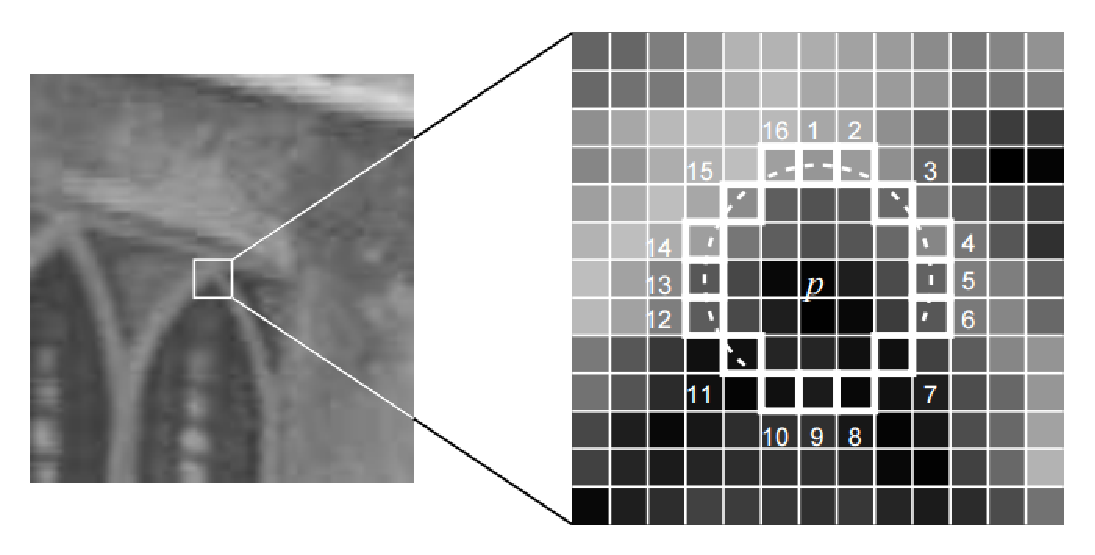
\includegraphics[width=0.9\linewidth]{vo1/fast-corner}
	\caption{FAST特征点\textsuperscript{\cite{Rosten2006}}。}
	\label{fig:fastcorner}
\end{figure}

FAST特征点的计算仅仅是比较像素间亮度的差异所所以速度非常快,但它也有重复性不强,分布不均匀的缺点。此外,FAST角点不具有方向信息。同时,由于它固定取半径为3的圆,存在尺度问题:远处看着像是角点的地方,接近后看可能就不是角点了。针对FAST角点不具有方向性和尺度的弱点,ORB添加了尺度和旋转的描述。尺度不变性由构建图像金字塔\footnote{金字塔是指对图像进行不同层次的降采样,以获得不同分辨率的图像。},并在金字塔的每一层上检测角点来实现。而特征的旋转是由灰度质心法(Intensity Centroid)实现的。

金字塔时计算图视觉中常用的一种处理方法,示意图见\autoref{fig:pyramid}。金字塔底层是原始图像。每往上一层,就对图像进行一个固定倍率的缩放,这样我们就有了不同分辨率的图像。较小的图像可以看成是远处看过来的场景。在特征匹配算法中,我们可以匹配不同层上的图像,从而实现尺度不变性。例如,如果相机在后退,那么我们应该能够在上一个图像金字塔的上层和下一个图像的下层中找到匹配。

\begin{figure}[!t]
    \centering
    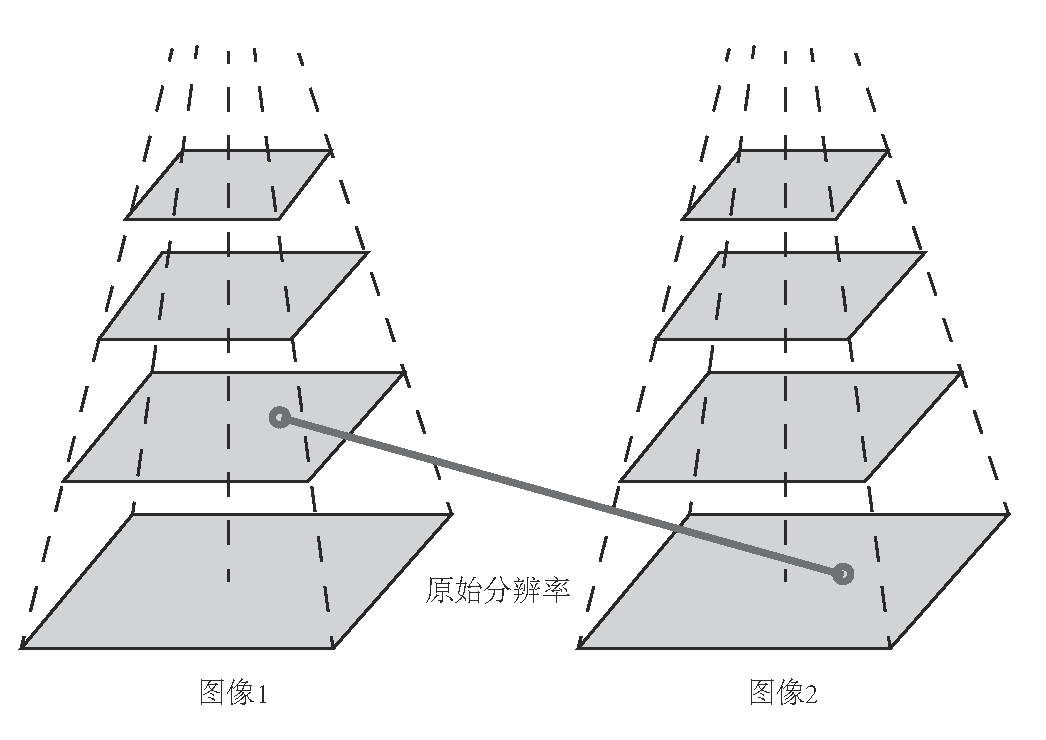
\includegraphics[width=0.9\linewidth]{vo1/pyramid}\\
    \caption{使用金字塔可以匹配不同缩放倍率下的图像。}
    \label{fig:pyramid}
\end{figure}

在旋转方面,我们计算特征点附近的图像灰度质心。所谓质心是指以图像块灰度值作为权重的中心。其具体操作步骤如下\textsuperscript{\cite{Rosin1999}}:
\begin{enumerate}
\item 在一个小的图像块$B$中,定义图像块的矩为
\[
m_{pq}=\sum_{x,y \in B}x^{p}y^{q}I(x,y), \quad p, q = \{0,1\}.
\]
\item 通过矩可以找到图像块的质心:
\[
C=\left(\frac{m_{10}}{m_{00}},\frac{m_{01}}{m_{00}}\right).
\]
\item 连接图像块的几何中心$O$与质心$C$,得到一个方向向量$\overrightarrow{OC}$,于是特征点的方向可以定义为
\[
\theta = \arctan(m_{01}/m_{10}).
\]
\end{enumerate}
通过以上方法,FAST角点便具有了尺度与旋转的描述,从而大大提升了其在不同图像之间表述的鲁棒性。所以在ORB中,把这种改进后的FAST称为Oriented FAST。

\subsubsection{BRIEF描述子}
在提取Oriented FAST关键点后,我们对每个点计算其描述子。ORB使用改进的BRIEF特征描述。我们先来介绍一下BRIEF是什么。

BRIEF是一种\textbf{二进制}描述子,其描述向量由许多个0和1组成,这里的0和1编码了关键点附近两个随机像素(比如$p$和$q$)的大小关系:如果$p$比$q$大,则取1,反之就取0。如果我们取了128个这样的$p,q$,最后就得到128维由0、1组成的向量\textsuperscript{\cite{calonder2010brief}}。BRIEF使用了随机选点的比较,速度非常快,而且由于使用了二进制表达,存储起来也十分方便,适用于实时的图像匹配。原始的BRIEF描述子不具有旋转不变性,因此在图像发生旋转时容易丢失。而ORB在FAST特征点提取阶段计算了关键点的方向,所以可以利用方向信息,计算了旋转之后的“Steer BRIEF”特征使ORB的描述子具有较好的旋转不变性。

由于考虑到了旋转和缩放,使得ORB在平移、旋转和缩放的变换下仍有良好的表现。同时,FAST和BREIF的组合也非常高效,使得ORB特征在实时SLAM中非常受欢迎。我们在\autoref{fig:ORB}~中展示了一张图像提取ORB之后的结果,下面来介绍如何在不同的图像之间进行特征匹配。

\begin{figure}[!htp]
    \centering
    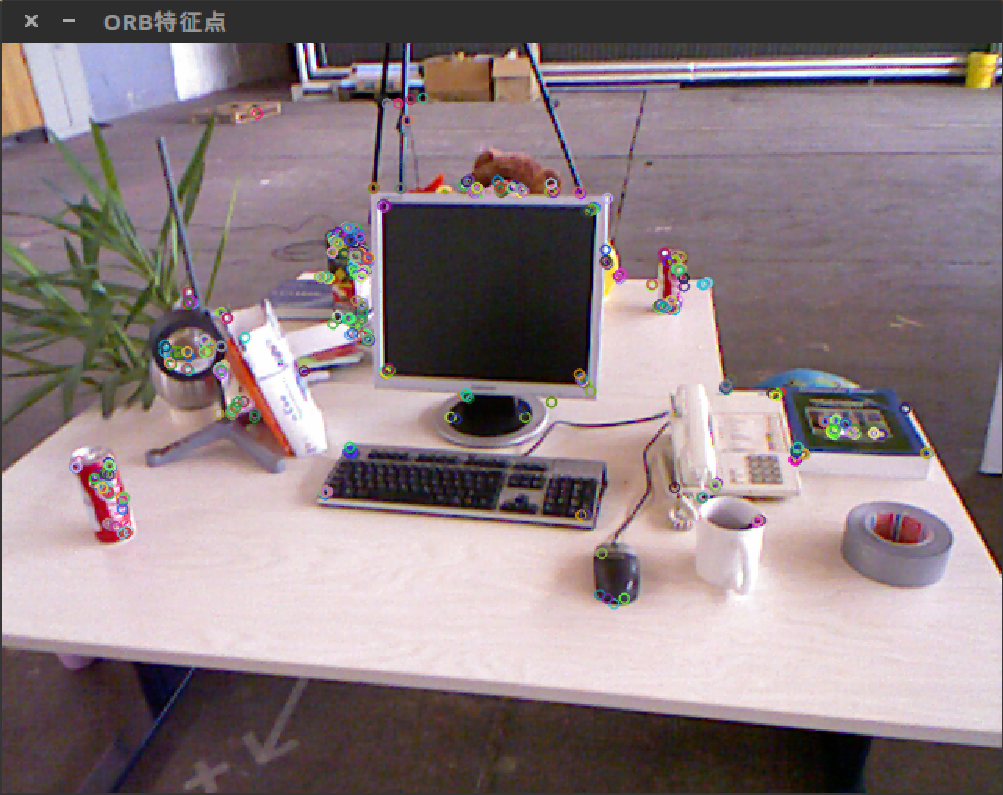
\includegraphics[width=0.9\linewidth]{vo1/feature}\\
    \caption{OpenCV提供的ORB特征点检测结果。}
    \label{fig:ORB}
\end{figure}

\subsection{特征匹配}

特征匹配(如\autoref{fig:feature-matching}~所示)是视觉SLAM中极为关键的一步,宽泛地说,特征匹配解决了SLAM中的数据关联问题(data association),即确定当前看到的路标与之前看到的路标之间的对应关系。通过对图像与图像或者图像与地图之间的描述子进行准确匹配,我们可以为后续的姿态估计、优化等操作减轻大量负担。然而,由于图像特征的局部特性,误匹配的情况广泛存在,而且长期以来一直没有得到有效解决,目前已经成为视觉SLAM中制约性能提升的一大瓶颈。部分原因是场景中经常存在大量的重复纹理,使得特征描述非常相似。在这种情况下,仅利用局部特征解决误匹配是非常困难的。

\begin{figure}[!htp]
    \centering
    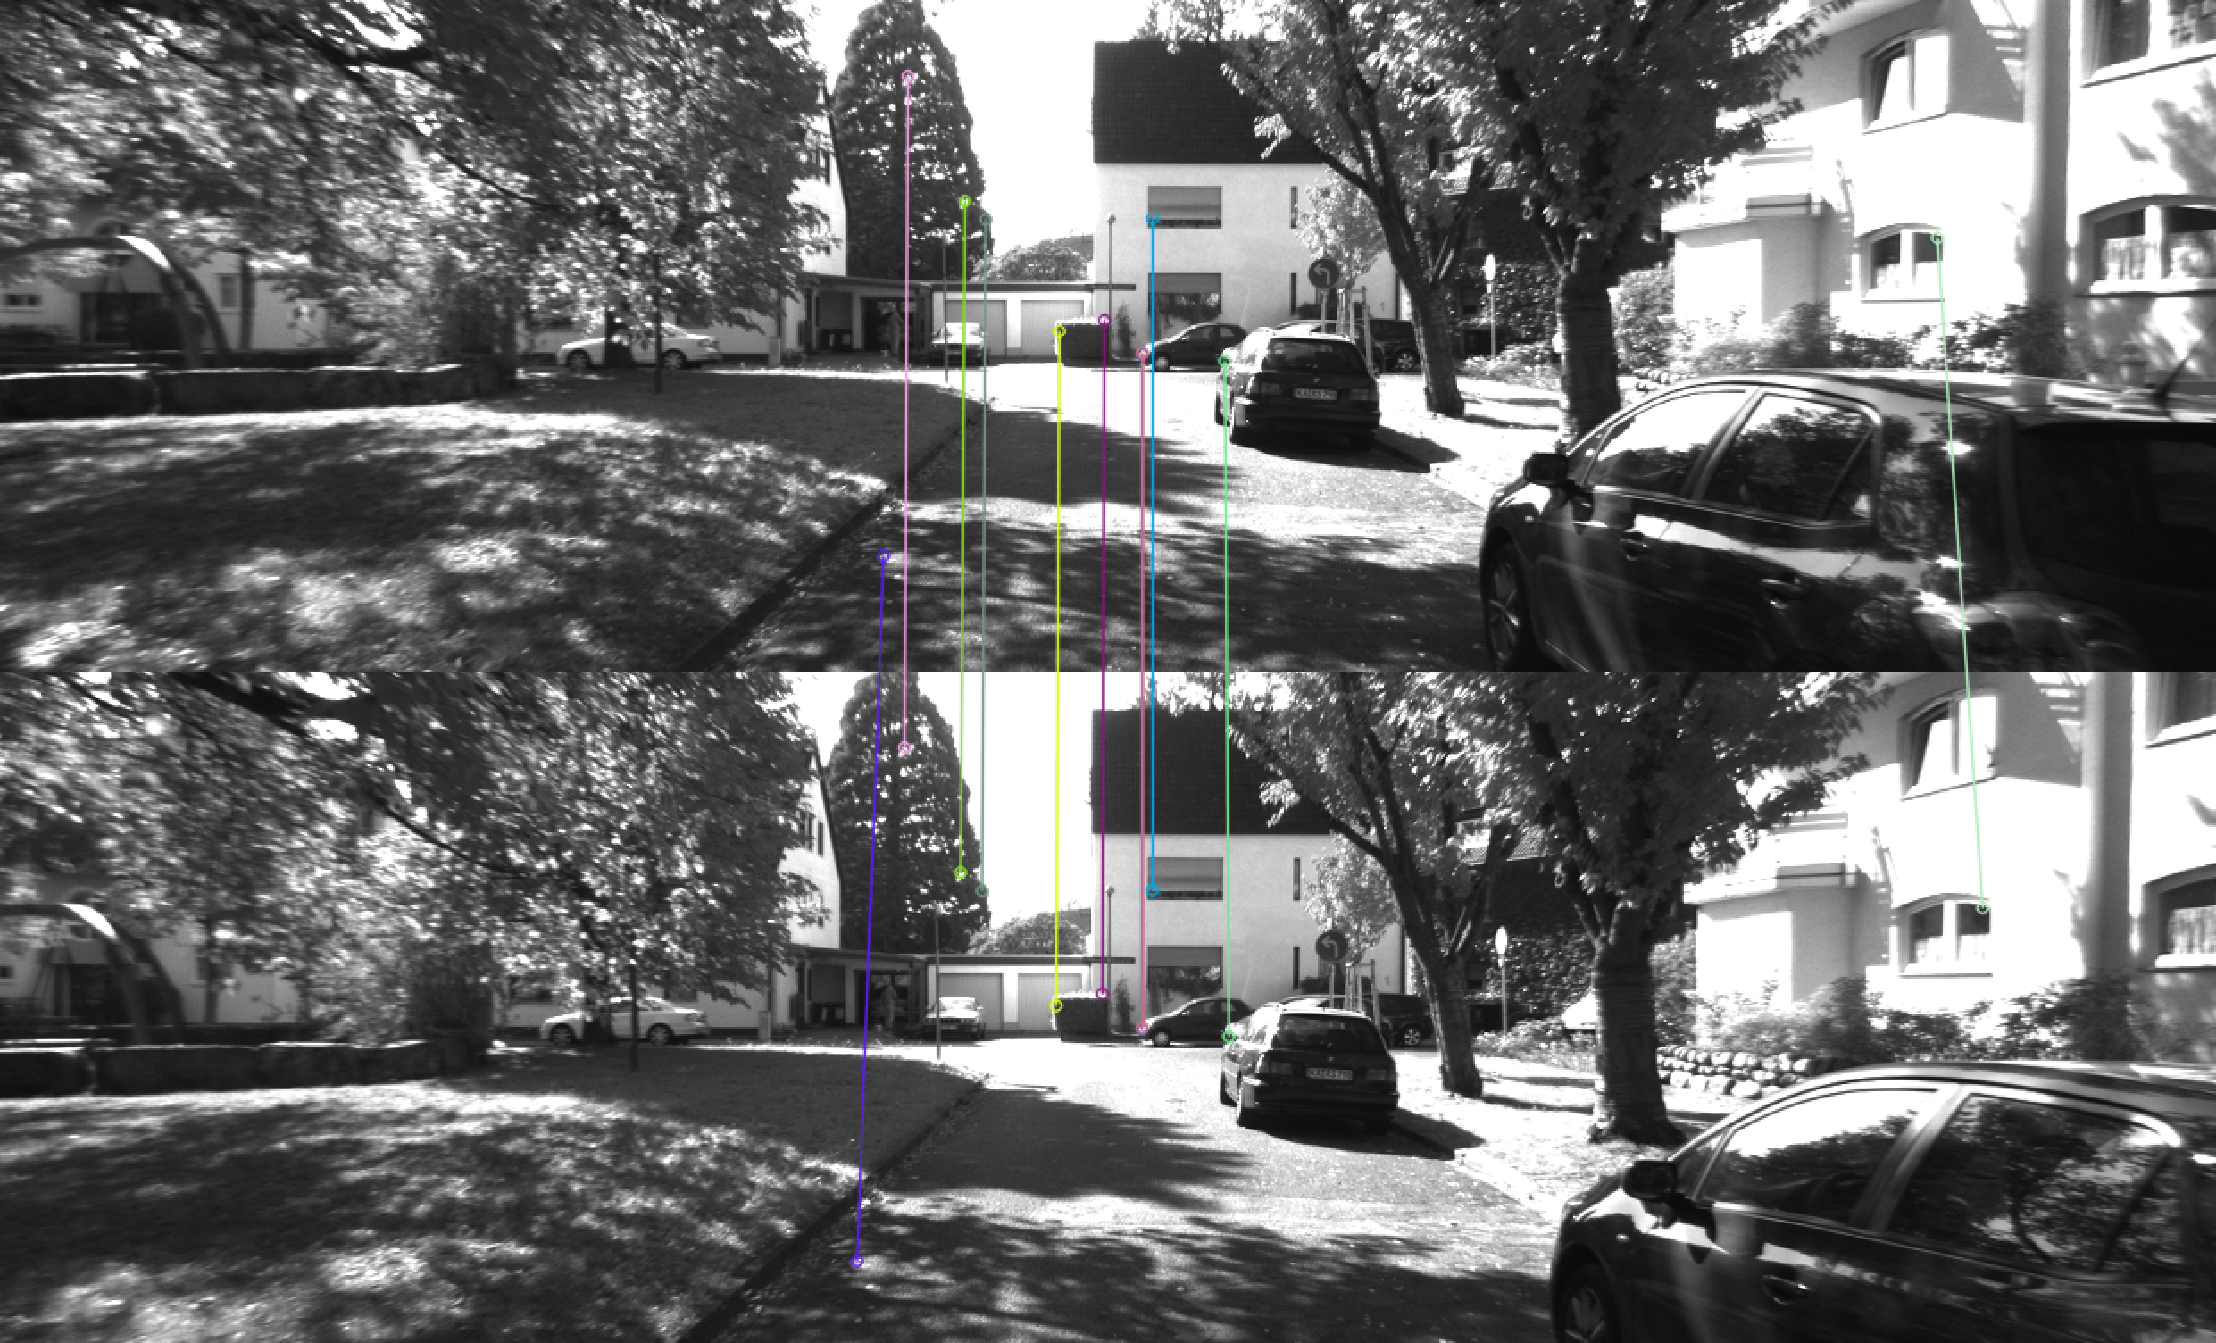
\includegraphics[width=0.9\linewidth]{vo1/feature-matching}
    \caption{两帧图像间的特征匹配。}
    \label{fig:feature-matching}
\end{figure}

不过,让我们先来看正确匹配的情况,等做完实验再回头去讨论误匹配问题。考虑两个时刻的图像。如果在图像$I_{t}$中提取到特征点$ x_{t}^{m}, m=1,2,...,M$,在图像$I_{t+1}$中提取到特征点$x_{t+1}^{n}, n=1,2,...,N$,如何寻找这两个集合元素的对应关系呢?最简单的特征匹配方法就是\textbf{暴力匹配(Brute-Force Matcher)}。即对每一个特征点$x_{t}^{m}$与所有的$x_{t+1}^{n}$测量描述子的距离,然后排序,取最近的一个作为匹配点。描述子距离表示了两个特征之间的\textbf{相似程度},不过在实际运用中还可以取不同的距离度量范数。对于浮点类型的描述子,使用欧氏距离进行度量即可。而对于二进制的描述子(比如BRIEF这样的),我们往往使用汉明距离(Hamming distance)作为度量——两个二进制串之间的汉明距离,指的是其\textbf{不同位数的个数}。

然而,当特征点数量很大时,暴力匹配法的运算量将变得很大,特别是当想要匹配某个帧和一张地图的时候。这不符合我们在SLAM中的实时性需求。此时\textbf{快速近似最近邻(FLANN)}算法更加适合于匹配点数量极多的情况。由于这些匹配算法理论已经成熟,而且实现上也已集成到OpenCV,所以这里就不再描述它的技术细节了。感兴趣的读者可以参考阅读文献\cite{Muja2009}。

\section{实践:特征提取和匹配}
\begin{figure}[!htp]
	\centering
	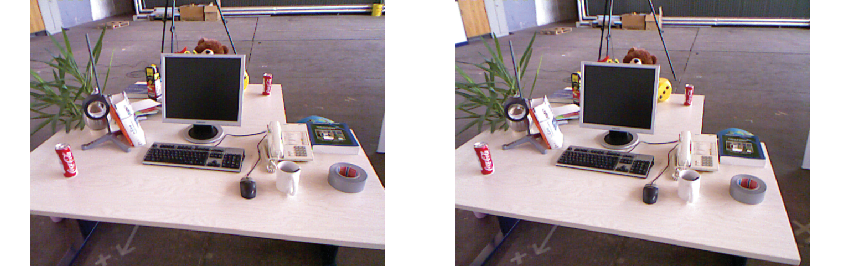
\includegraphics[width=0.9\linewidth]{vo1/exp1-images.pdf}
	\caption{实验使用的两帧图像。}
	\label{fig:exp1-images}
\end{figure}

OpenCV已经集成了多数主流的图像特征,我们可以很方便地进行调用。下面我们来完成两个实验:第一个实验中,我们演示使用OpenCV进行ORB的特征匹配;第二个实验中,我们演示如何根据前面介绍的原理,手写一个简单的ORB特征。通过手写的过程,读者可以更加清楚地理解ORB的计算过程,并类推到其他特征上去。

\subsection{OpenCV的ORB特征}
首先我们调用OpenCV来提取和匹配ORB。我为此实验准备了两张图像,位于slambook2/ch7/下的1.png和2.png,如\autoref{fig:exp1-images}~所示。它们是来自公开数据集\cite{Sturm2012}中的两张图像,我们看到相机发生了微小的运动。本节程序演示如何提取ORB特征并进行匹配。下一小节中,我们将演示如何用匹配结果来估计相机运动。

下面程序演示了ORB的使用方法:
\begin{lstlisting}[language=c++,caption=slambook2/ch7/orb_cv.cpp]
#include <iostream>
#include <opencv2/core/core.hpp>
#include <opencv2/features2d/features2d.hpp>
#include <opencv2/highgui/highgui.hpp>
#include <chrono>

using namespace std;
using namespace cv;

int main(int argc, char **argv) {
    if (argc != 3) {
        cout << "usage: feature_extraction img1 img2" << endl;
        return 1;
    }
    //-- 读取图像
    Mat img_1 = imread(argv[1], CV_LOAD_IMAGE_COLOR);
    Mat img_2 = imread(argv[2], CV_LOAD_IMAGE_COLOR);
    assert(img_1.data != nullptr && img_2.data != nullptr);
    
    //-- 初始化
    std::vector<KeyPoint> keypoints_1, keypoints_2;
    Mat descriptors_1, descriptors_2;
    Ptr<FeatureDetector> detector = ORB::create();
    Ptr<DescriptorExtractor> descriptor = ORB::create();
    Ptr<DescriptorMatcher> matcher = DescriptorMatcher::create("BruteForce-Hamming");
    
    //-- 第一步:检测 Oriented FAST 角点位置
    chrono::steady_clock::time_point t1 = chrono::steady_clock::now();
    detector->detect(img_1, keypoints_1);
    detector->detect(img_2, keypoints_2);
    
    //-- 第二步:根据角点位置计算 BRIEF 描述子
    descriptor->compute(img_1, keypoints_1, descriptors_1);
    descriptor->compute(img_2, keypoints_2, descriptors_2);
    chrono::steady_clock::time_point t2 = chrono::steady_clock::now();
    chrono::duration<double> time_used = chrono::duration_cast<chrono::duration<double>>(t2 - t1);
    cout << "extract ORB cost = " << time_used.count() << " seconds. " << endl;
    
    Mat outimg1;
    drawKeypoints(img_1, keypoints_1, outimg1, Scalar::all(-1), DrawMatchesFlags::DEFAULT);
    imshow("ORB features", outimg1);
    
    //-- 第三步:对两幅图像中的BRIEF描述子进行匹配,使用 Hamming 距离
    vector<DMatch> matches;
    t1 = chrono::steady_clock::now();
    matcher->match(descriptors_1, descriptors_2, matches);
    t2 = chrono::steady_clock::now();
    time_used = chrono::duration_cast<chrono::duration<double>>(t2 - t1);
    cout << "match ORB cost = " << time_used.count() << " seconds. " << endl;
    
    //-- 第四步:匹配点对筛选
    // 计算最小距离和最大距离
    auto min_max = minmax_element(matches.begin(), matches.end(),
        [](const DMatch &m1, const DMatch &m2) { return m1.distance < m2.distance; });
    double min_dist = min_max.first->distance;
    double max_dist = min_max.second->distance;
    
    printf("-- Max dist : %f \n", max_dist);
    printf("-- Min dist : %f \n", min_dist);
    
    //当描述子之间的距离大于两倍的最小距离时,即认为匹配有误.但有时候最小距离会非常小,设置一个经验值30作为下限.
    std::vector<DMatch> good_matches;
    for (int i = 0; i < descriptors_1.rows; i++) {
        if (matches[i].distance <= max(2 * min_dist, 30.0)) {
            good_matches.push_back(matches[i]);
        }
    }
    
    //-- 第五步:绘制匹配结果
    Mat img_match;
    Mat img_goodmatch;
    drawMatches(img_1, keypoints_1, img_2, keypoints_2, matches, img_match);
    drawMatches(img_1, keypoints_1, img_2, keypoints_2, good_matches, img_goodmatch);
    imshow("all matches", img_match);
    imshow("good matches", img_goodmatch);
    waitKey(0);
    
    return 0;
}
\end{lstlisting}

运行此程序(需要输入两个图像位置),将输出运行结果:
\begin{lstlisting}[language=sh,caption=终端输入:]
% build/orb_cv 1.png 2.png
extract ORB cost = 0.0229183 seconds. 
match ORB cost = 0.000751868 seconds.
-- Max dist : 95.000000 
-- Min dist : 4.000000 
\end{lstlisting}

\autoref{fig:exp1-results}~显示了例程的运行结果。我们看到未筛选的匹配中带有大量的误匹配。经过一次筛选之后,匹配数量减少了许多,但大多数匹配都是正确的。这里,筛选的依据是\textbf{汉明距离小于最小距离的两倍},这是一种工程上的经验方法,不一定有理论依据。不过,尽管在示例图像中能够筛选出正确的匹配,但我们仍然不能保证在所有其他图像中得到的匹配都是正确的。因此,在后面的运动估计中,还需要使用去除误匹配的算法。在我的机器上,ORB提取花费了22.9毫秒(两张图像),匹配花费了0.75毫秒,可见大部分计算量花在了特征提取上。

\begin{figure}[!htp]
	\centering
	\includegraphics[width=1.0\linewidth]{vo1/exp1-result}
	\caption{特征提取与匹配结果。}
	\label{fig:exp1-results} 
\end{figure}

\subsection{手写ORB特征}
下面我们演示手写ORB特征的方法。这部分代码比较多,书上只展示核心部分的代码,其余的周边代码请读者从代码库中获取。
\begin{lstlisting}[language=c++,caption=slambook2/ch7/orb_self.cpp(片段)]
typedef vector<uint32_t> DescType;
// ... 省略图片读取部分代码和测试代码
// compute the descriptor
void ComputeORB(const cv::Mat &img, vector<cv::KeyPoint> &keypoints, vector<DescType> &descriptors) {
    const int half_patch_size = 8;
    const int half_boundary = 16;
    int bad_points = 0;
    for (auto &kp: keypoints) {
        if (kp.pt.x < half_boundary || kp.pt.y < half_boundary ||
        kp.pt.x >= img.cols - half_boundary || kp.pt.y >= img.rows - half_boundary) {
            // outside
            bad_points++;
            descriptors.push_back({});
            continue;
        }
    
        float m01 = 0, m10 = 0;
        for (int dx = -half_patch_size; dx < half_patch_size; ++dx) {
            for (int dy = -half_patch_size; dy < half_patch_size; ++dy) {
                uchar pixel = img.at<uchar>(kp.pt.y + dy, kp.pt.x + dx);
                m01 += dx * pixel;
                m10 += dy * pixel;
            }
        }
    
        // angle should be arc tan(m01/m10);
        float m_sqrt = sqrt(m01 * m01 + m10 * m10);
        float sin_theta = m01 / m_sqrt;
        float cos_theta = m10 / m_sqrt;
        
        // compute the angle of this point
        DescType desc(8, 0);
        for (int i = 0; i < 8; i++) {
            uint32_t d = 0;
            for (int k = 0; k < 32; k++) {
                int idx_pq = i * 8 + k;
                cv::Point2f p(ORB_pattern[idx_pq * 4], ORB_pattern[idx_pq * 4 + 1]);
                cv::Point2f q(ORB_pattern[idx_pq * 4 + 2], ORB_pattern[idx_pq * 4 + 3]);
        
                // rotate with theta
                cv::Point2f pp = cv::Point2f(cos_theta * p.x - sin_theta * p.y, sin_theta * p.x + cos_theta * p.y) + kp.pt;
                cv::Point2f qq = cv::Point2f(cos_theta * q.x - sin_theta * q.y, sin_theta * q.x + cos_theta * q.y) + kp.pt;
                if (img.at<uchar>(pp.y, pp.x) < img.at<uchar>(qq.y, qq.x)) {
                    d |= 1 << k;
                }
            }
            desc[i] = d;
        }
        descriptors.push_back(desc);
    }
    
    cout << "bad/total: " << bad_points << "/" << keypoints.size() << endl;
}

// brute-force matching
void BfMatch(
    const vector<DescType> &desc1, const vector<DescType> &desc2, vector<cv::DMatch> &matches) {
    const int d_max = 40;
    
    for (size_t i1 = 0; i1 < desc1.size(); ++i1) {
        if (desc1[i1].empty()) continue;
        cv::DMatch m{i1, 0, 256};
        for (size_t i2 = 0; i2 < desc2.size(); ++i2) {
            if (desc2[i2].empty()) continue;
            int distance = 0;
            for (int k = 0; k < 8; k++) {
                distance += _mm_popcnt_u32(desc1[i1][k] ^desc2[i2][k]);
            }
            if (distance < d_max && distance < m.distance) {
                m.distance = distance;
                m.trainIdx = i2;
            }
        }
        if (m.distance < d_max) {
            matches.push_back(m);
        }
    }
}
\end{lstlisting}
这个演示中我们只展示ORB的计算代码和匹配代码。在计算中,我们用256位的二进制描述,即对应到8个32位的unsigned int数据,用typedef将它表示成DescType。然后,我们根据前面介绍的原理计算FAST特征点的角度,再使用该角度计算描述子。此代码中通过三角函数的原理回避了复杂的$\arctan$以及$\sin$、$\cos$计算,从而达到加速的效果。在BfMatch函数中,我们还使用了SSE指令集中的\_mm\_popcnt\_u32函数来计算一个unsigned int变量中1的个数,从而达到计算汉明距离的效果。该段程序的运行结果如下,匹配结果如\autoref{fig:matches}所示:

\begin{lstlisting}[language=sh,caption=终端输出:]
bad/total: 43/638
bad/total: 8/595
extract ORB cost = 0.00390721 seconds.
match ORB cost = 0.000862984 seconds.
matches: 51
\end{lstlisting}

\begin{figure}[!htp]
    \centering
    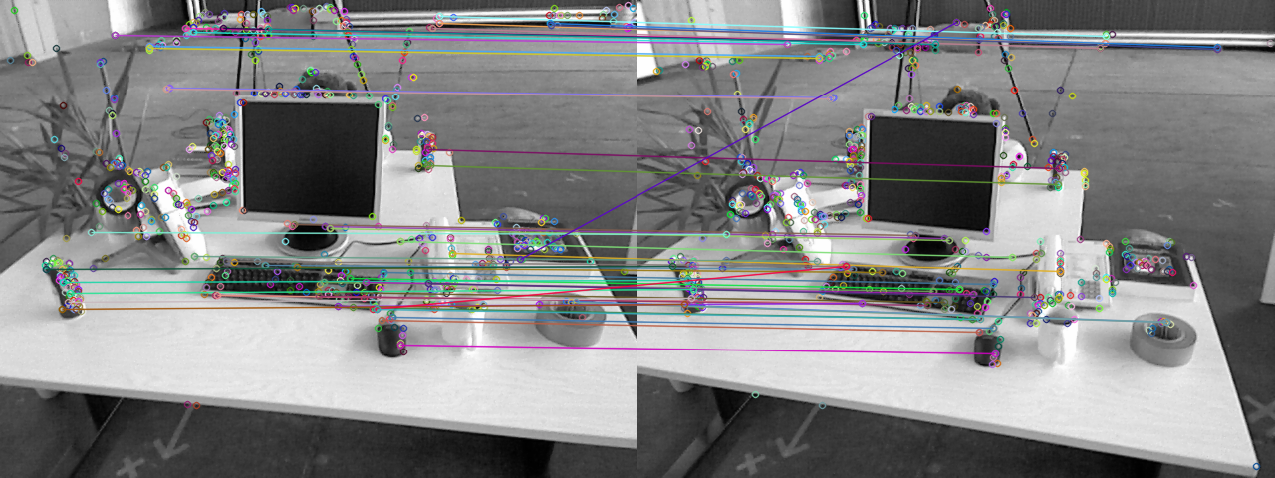
\includegraphics[width=0.8\linewidth]{vo1/matches}
    \caption{匹配结果}
    \label{fig:matches}
\end{figure}

可见,这个程序中,ORB的提取只需要3.9毫秒,匹配只需0.86毫秒。我们通过一些简单的算法修改,对ORB的提取加速了5.8倍。请读者注意,编译这个程序需要你的CPU支持SSE指令集,这应该在绝大多数现代的家用CPU上都已经支持。如果我们能够对提取特征部分进一步并行化处理,算法还可以有加速的空间。

\subsection{计算相机运动}
我们已经有了匹配好的点对,接下来,我们要根据点对来估计相机的运动。这里由于相机的原理不同,情况发生了变化:

\begin{enumerate}
	\item 当相机为单目时,我们只知道2D的像素坐标,因而问题是根据\textbf{两组2D点}估计运动。该问题用\textbf{对极几何}来解决。
	\item 当相机为双目、RGB-D时,或者通过某种方法得到了距离信息,那么问题就是根据\textbf{两组3D点}估计运动。该问题通常用ICP来解决。
	\item 如果一组为3D,一组为2D,即,我们得到了一些3D点和它们在相机的投影位置,也能估计相机的运动。该问题通过\textbf{PnP}求解。
\end{enumerate}

因此,下面几节就来介绍这三种情形下的相机运动估计。我们将从信息最少的2D−2D情形出发,看看它如何求解,求解过程又有哪些麻烦的问题。

\section{2D−2D: 对极几何}
\label{sec:epipolar-geometry}

\subsection{对极约束}

现在,假设我们从两张图像中得到了一对配对好的特征点,如\autoref{fig:doubleview}~所示。如果有若干对这样的匹配点,就可以通过这些二维图像点的对应关系,恢复出在两帧之间摄像机的运动。这里“若干对”具体是多少对呢?我们会在下文介绍。下面先来看看两个图像当中的匹配点有什么几何关系。

\begin{figure}[!htp]
	\centering
	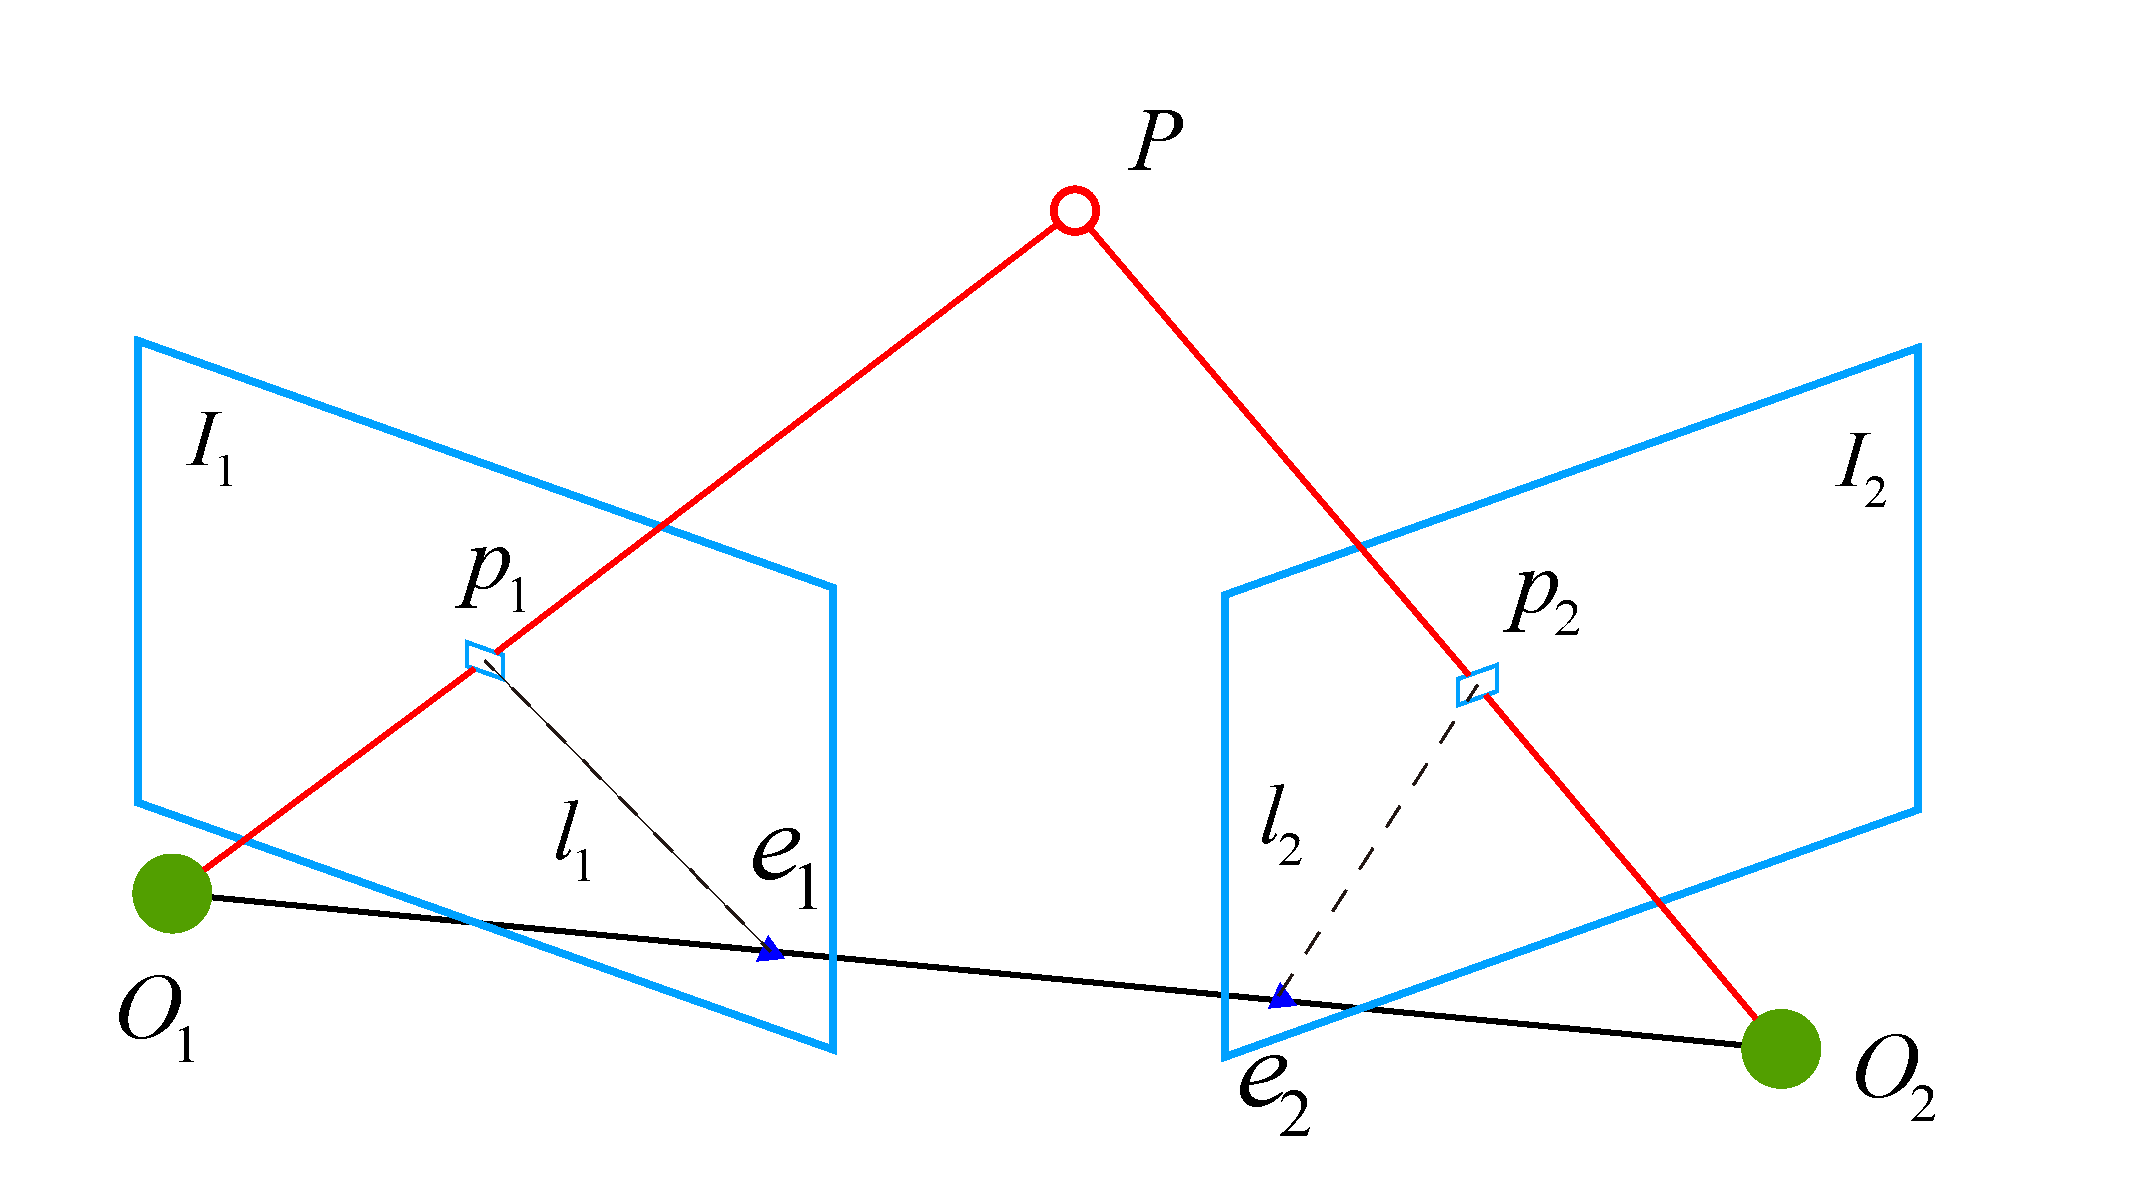
\includegraphics[width=0.6\linewidth]{vo1/fundamental}
	\caption{对极几何约束。}
	\label{fig:doubleview}
\end{figure}

以\autoref{fig:doubleview}~为例,我们希望求取两帧图像$I_{1}, I_{2}$之间的运动,设第一帧到第二帧的运动为$\bm{R}, \bm{t}$。两个相机中心分别为$O_{1}, O_{2}$。现在,考虑$I_{1}$中有一个特征点$p_{1}$,它在$I_{2}$中对应着特征点$p_{2}$。我们知道两者是通过特征匹配得到的。如果匹配正确,说明它们确实是\textbf{同一个空间点在两个成像平面上的投影}。这里需要一些术语来描述它们之间的几何关系。首先,连线$\overrightarrow{O_{1}p_{1}}$和连线$\overrightarrow{O_{2}p_{2}}$在三维空间中会相交于点$P$。这时候点$O_{1},O_{2},P$三个点可以确定一个平面,称为\textbf{极平面(Epipolar plane)}。$O_{1}O_{2}$连线与像平面$I_{1},I_{2}$的交点分别为$e_{1},e_{2}$。$e_{1},e_{2}$称为\textbf{极点(Epipoles)},$O_{1}O_{2}$被称为\textbf{基线(Baseline)}。我们称极平面与两个像平面$I_{1}, I_{2}$之间的相交线$l_{1},l_{2}$为\textbf{极线(Epipolar line)}。

直观讲,从第一帧的角度看,射线$\overrightarrow{O_1 p_1}$是\textbf{某个像素可能出现的空间位置}——因为该射线上的所有点都会投影到同一个像素点。同时,如果不知道$P$的位置,那么当我们在第二幅图像上看时,连线$\overrightarrow{e_2 p_2}$(也就是第二幅图像中的极线)就是$P$可能出现的投影的位置,也就是射线$\overrightarrow{O_1 p_1}$在第二个相机中的投影。现在,由于我们通过特征点匹配确定了$p_2$的像素位置,所以能够推断$P$的空间位置,以及相机的运动。要提醒读者的是,\textbf{这多亏了正确的特征匹配}。如果没有特征匹配,我们就没法确定$p_2$到底在极线的哪个位置了。那时,就必须在极线上搜索以获得正确的匹配,这将在第12讲中提到。

现在,我们从代数角度来看一下这里的几何关系。在第一帧的坐标系下,设$P$的空间位置为
\[
\bm{P}=[X,Y,Z]^\mathrm{T}.
\]
根据第5讲介绍的针孔相机模型,我们知道两个像素点$\bm{p}_1,\bm{p}_2$的像素位置为
\begin{equation}
s_1 {\bm{p}_1} = \bm{KP},\quad s_2 \bm{p}_2 = \bm{K}\left( \bm{RP + t} \right).
\end{equation}

这里$\bm{K}$为相机内参矩阵,$\bm{R}, \bm{t}$为两个坐标系的相机运动。具体来说,这里计算的是$\bm{R}_{21}$和$\bm{t}_{21}$,因为它们把第一个坐标系下的坐标转换到第二个坐标系下。如果我们愿意,也可以把它们写成李代数形式。

有时候,我们会使用齐次坐标表示像素点。在使用齐次坐标时,一个向量将等于它自身乘上任意的非零常数。这通常用于表达一个投影关系。例如$s_1 \bm{p}_1$和$\bm{p}_1$成投影关系,它们在齐次坐标的意义下是相等的。我们称这种相等关系为\textbf{尺度意义下相等}(equal up to a scale),记作:
\begin{equation}
s\bm{p} \simeq \bm{p}.
\end{equation}
那么,上述两个投影关系可写为:
\begin{equation}
 {\bm{p}_1} \simeq \bm{KP},\quad \bm{p}_2 \simeq \bm{K}\left( \bm{RP + t} \right).
\end{equation}

现在,取:
\begin{equation}
{\bm{x}_1} = {\bm{K}^{ - 1}}{\bm{p}_1}, \quad {\bm{x}_2} = {\bm{K}^{ - 1}}{\bm{p}_2}.
\end{equation}

这里的$\bm{x}_1, \bm{x}_2$是两个像素点的归一化平面上的坐标。代入上式,得:
\begin{equation}
{\bm{x}_2} \simeq \bm{R} {\bm{x}_1} + \bm{t}.
\end{equation}

两边同时左乘$\bm{t}^\wedge$。回忆$^\wedge$的定义,这相当于两侧同时与$\bm{t}$做外积:
\begin{equation}
\bm{t}^\wedge \bm{x}_2 \simeq \bm{t}^\wedge \bm{R} \bm{x}_1.
\end{equation}

然后,两侧同时左乘$\bm{x}_2^\mathrm{T}$:
\begin{equation}
\bm{x}_2^\mathrm{T} \bm{t}^\wedge \bm{x}_2 \simeq \bm{x}_2^\mathrm{T} \bm{t}^\wedge \bm{R} \bm{x}_1.
\end{equation}

观察等式左侧,$\bm{t}^\wedge \bm{x}_2$是一个与$\bm{t}$和$\bm{x}_2$都垂直的向量。把它再和$\bm{x}_2$做内积时,将得到0。由于等式左侧严格为零,那么乘以任意非零常数之后也为零,于是我们可以把$\simeq$写成通常的等号。因此,我们就得到了一个简洁的式子:
\begin{equation}
 \bm{x}_2^\mathrm{T} \bm{t}^\wedge \bm{R} \bm{x}_1 = 0.
\end{equation}

重新代入$\bm{p}_1, \bm{p}_2$,有:
\begin{equation}
\bm{p}_2^\mathrm{T} \bm{K}^{-\mathrm{T}} \bm{t}^\wedge \bm{R} \bm{K}^{-1} \bm{p}_1  = 0.
\end{equation}

这两个式子都称为\textbf{对极约束},它以形式简洁著名。它的几何意义是$O_1, P, O_2$三者共面。对极约束中同时包含了平移和旋转。我们把中间部分记作两个矩阵:基础矩阵(Fundamental Matrix)$\bm{F}$和本质矩阵(Essential Matrix)$\bm{E}$,于是可以进一步简化对极约束:
\begin{equation}
\bm{E} = \bm{t}^ \wedge \bm{R}, \quad \bm{F} = \bm{K}^{ -\mathrm{T}} \bm{E} {\bm{K}^{ - 1}}, \quad \bm{x}_2^\mathrm{T} \bm{E} {\bm{x}_1} = \bm{p}_2^\mathrm{T} \bm{F} {\bm{p}_1} = 0.
\end{equation}

对极约束简洁地给出了两个匹配点的空间位置关系。于是,相机位姿估计问题变为以下两步:

\begin{enumerate}
	\item 根据配对点的像素位置求出$\bm{E}$或者$\bm{F}$。
	\item 根据$\bm{E}$或者$\bm{F}$求出$\bm{R}, \bm{t}$。
\end{enumerate}

由于$\bm{E}$和$\bm{F}$只相差了相机内参,而内参在SLAM中通常是已知的\footnote{在SfM研究中则有可能是未知而有待估计的。},所以实践当中往往使用形式更简单的$\bm{E}$。我们以$\bm{E}$为例,介绍上面两个问题如何求解。

\subsection{本质矩阵}
根据定义,本质矩阵$\bm{E} = \bm{t}^\wedge \bm{R}$。它是一个$3\times 3$的矩阵,内有9个未知数。那么,是不是任意一个$3 \times 3$的矩阵都可以被当成本质矩阵呢?从$\bm{E}$的构造方式上看,有以下值得注意的地方:

\begin{itemize}
	\item 本质矩阵是由对极约束定义的。由于对极约束是\textbf{等式为零}的约束,所以对$\bm{E}$乘以任意非零常数后,\textbf{对极约束依然满足}。我们把这件事情称为$\bm{E}$在不同尺度下是等价的。
	\item 根据$\bm{E} = \bm{t}^ \wedge \bm{R}$,可以证明\textsuperscript{\cite{Hartley2003}},本质矩阵$\bm{E}$的奇异值必定是$[\sigma, \sigma, 0]^\mathrm{T}$的形式。这称为\textbf{本质矩阵的内在性质}。
	\item 另一方面,由于平移和旋转各有3个自由度,故$\bm{t}^\wedge \bm{R}$共有6个自由度。但由于尺度等价性,故$\bm{E}$实际上有5个自由度。
\end{itemize}

$\bm{E}$具有5个自由度的事实,表明我们最少可以用5对点来求解$\bm{E}$。但是,$\bm{E}$的内在性质是一种非线性性质,在估计时会带来麻烦,因此,也可以只考虑它的\textbf{尺度等价性},使用8对点来估计$\bm{E}$——这就是经典的\textbf{八点法(Eight-point-algorithm)}\textsuperscript{\cite{Hartley1997, Longuet-Higgins1987}}。八点法只利用了$\bm{E}$的线性性质,因此可以在线性代数框架下求解。下面我们来看八点法是如何工作的。

考虑一对匹配点,它们的归一化坐标为$\bm{x}_{1}=[u_{1},v_{1},1]^\mathrm{T}$, $\bm{x}_{2}=[u_{2},v_{2},1]^{\mathrm{T}}$。根据对极约束,有:
\begin{equation}
\begin{pmatrix} 
u_{2},v_{2},1
\end{pmatrix}
\begin{pmatrix}
 e_{1} & e_{2} & e_{3}\\ 
 e_{4} & e_{5} & e_{6}\\ 
 e_{7} & e_{8} & e_{9} 
\end{pmatrix}
\begin{pmatrix} 
u_{1}\\v_{1}\\1
\end{pmatrix}
=0.
\end{equation}

我们把矩阵$\bm{E}$展开,写成向量的形式:
\[
\bm{e}= [e_{1},e_{2},e_{3},e_{4},e_{5},e_{6},e_{7},e_{8},e_{9}]^{\mathrm{T}},
\]
那么对极约束可以写成与$\bm{e}$有关的线性形式:
\begin{equation}
[u_{2}u_{1},u_{2}v_{1},u_{2},v_{2}u_{1},v_{2}v_{1},v_{2},u_{1},v_{1},1] \cdot  \bm{e}=0.
\end{equation}

同理,对于其他点对也有相同的表示。我们把所有点都放到一个方程中,变成线性方程组($u^i, v^i$表示第$i$个特征点,依此类推):
\begin{equation}
\label{Eq:eight-point}
\begin{pmatrix}
u_{2}^{1}u_{1}^{1}& u_{2}^{1}v_{1}^{1}& u_{2}^{1}& v_{2}^{1}u_{1}^{1}& v_{2}^{1}v_{1}^{1}& v_{2}^{1} &u_{1}^{1} &v_{1}^{1}&1\\
u_{2}^{2}u_{1}^{2}& u_{2}^{2}v_{1}^{2}& u_{2}^{2}& v_{2}^{2}u_{1}^{2}& v_{2}^{2}v_{1}^{2}& v_{2}^{2} &u_{1}^{2} &v_{1}^{2}&1\\
\vdots & \vdots & \vdots & \vdots & \vdots & \vdots & \vdots & \vdots \\
u_{2}^{8}u_{1}^{8}& u_{2}^{8}v_{1}^{8}& u_{2}^{8}& v_{2}^{8}u_{1}^{8}& v_{2}^{8}v_{1}^{8}& v_{2}^{8} &u_{1}^{8}&v_{1}^{8}&1\\
\end{pmatrix}
\begin{pmatrix}
e_{1}\\ e_{2}\\ e_{3}\\  e_{4}\\ e_{5}\\ e_{6}\\ e_{7}\\ e_{8}\\ e_{9}  
\end{pmatrix}
=0.
\end{equation}

这8个方程构成了一个线性方程组。它的系数矩阵由特征点位置构成,大小为$8 \times 9$。$\bm{e}$位于该矩阵的零空间中。如果系数矩阵是满秩的(即秩为8),那么它的零空间维数为1,也就是$\bm{e}$构成一条线。这与$\bm{e}$的尺度等价性是一致的。如果8对匹配点组成的矩阵满足秩为8的条件,那么$\bm{E}$的各元素就可由上述方程解得。

接下来的问题是如何根据已经估得的本质矩阵$\bm{E}$,恢复出相机的运动$\bm{R}, \bm{t}$。这个过程是由奇异值分解(SVD)得到的。设$\bm{E}$的SVD分解为
\begin{equation}
\bm{E} = \bm{U} \bm{\Sigma} \bm{V}^\mathrm{T},
\end{equation}
其中$\bm{U}, \bm{V}$为正交阵,$\bm{\Sigma}$为奇异值矩阵。根据$\bm{E}$的内在性质,我们知道$\bm{\Sigma} = \mathrm{diag}( \sigma, \sigma, 0 )$。在SVD分解中,对于任意一个$\bm{E}$,存在两个可能的$\bm{t}, \bm{R}$与它对应:
\begin{equation}
\begin{array}{l}
\bm{t}_1^ \wedge  = \bm{U}{\bm{R}_Z}(\frac{\pi }{2}) \bm{\Sigma} {\bm{U}^\mathrm{T}}, \quad {\bm{R}_1} = \bm{U} \bm{R}_Z^\mathrm{T}(\frac{\pi }{2}){ \bm{V}^\mathrm{T}}\\
\bm{t}_2^ \wedge  = \bm{U}{\bm{R}_Z}( - \frac{\pi }{2})\bm{\Sigma} {\bm{U}^\mathrm{T}}, \quad  {\bm{R}_2} = \bm{U} \bm{R}_Z^\mathrm{T}( - \frac{\pi }{2}){\bm{V}^\mathrm{T}}.
\end{array}
\end{equation}

其中$\bm{R}_Z\left(\frac{\pi }{2}\right)$表示沿$Z$轴旋转$90^\circ$得到的旋转矩阵。同时,由于$-\bm{E}$和$\bm{E}$等价,所以对任意一个$\bm{t}$取负号,也会得到同样的结果。因此,从$\bm{E}$分解到$\bm{t}, \bm{R}$时,一共存在\textbf{4个}可能的解。

\autoref{fig:epipolar-solution}~形象地展示了分解本质矩阵得到的4个解。我们已知空间点在相机(蓝色线)上的投影(红色点),想要求解相机的运动。在保持红色点不变的情况下,可以画出4种可能的情况。不过幸运的是,只有第一种解中$P$在两个相机中都具有正的深度。因此,只要把任意一点代入4种解中,检测该点在两个相机下的深度,就可以确定哪个解是正确的了。

\begin{figure}[!htp]
	\centering
	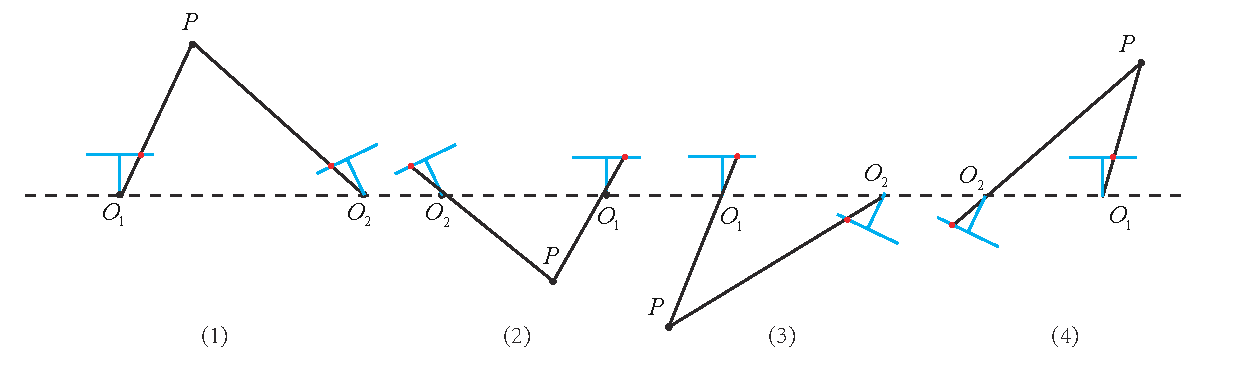
\includegraphics[width=1.0\linewidth]{vo1/epipolar-solution}
	\caption{分解本质矩阵得到的4个解。在保持投影点(红色点)不变的情况下,两个相机及空间点一共有4种可能的情况。}
	\label{fig:epipolar-solution}
\end{figure}

如果利用$\bm{E}$的内在性质,那么它只有5个自由度。所以最少可以通过5对点来求解相机运动\textsuperscript{\cite{Li2006, Nister2004a}}。然而这种做法形式复杂,从工程实现角度考虑,由于平时通常会有几十对乃至上百对的匹配点,从8对减至5对意义并不明显。为保持简单,我们这里就只介绍基本的八点法。

剩下的问题还有一个:根据线性方程解出的$\bm{E}$,可能不满足$\bm{E}$的内在性质——它的奇异值不一定为${\sigma}, {\sigma}, 0$的形式。这时,我们会刻意地把$\bm{\Sigma}$矩阵调整成上面的样子。通常的做法是,对八点法求得的$\bm{E}$进行SVD分解后,会得到奇异值矩阵$\bm{\Sigma} =  \mathrm{diag} ( \sigma_1, \sigma_2, \sigma_3)$,不妨设$\sigma_1 \geqslant \sigma_2 \geqslant \sigma_3$。取:
\begin{equation}
\bm{E} = \bm{U} \mathrm{diag} (\frac{\sigma_1+\sigma_2}{2}, \frac{\sigma_1+\sigma_2}{2}, 0) \bm{V}^\mathrm{T}.
\end{equation}
这相当于是把求出来的矩阵投影到了$\bm{E}$所在的流形上。当然,更简单的做法是将奇异值矩阵取成$\mathrm{diag} (1,1,0)$,因为$\bm{E}$具有尺度等价性,所以这样做也是合理的。

\subsection{单应矩阵}
除了基本矩阵和本质矩阵,二视图几何中还存在另一种常见的矩阵:单应矩阵(Homography)$\bm{H}$,它描述了两个平面之间的映射关系。若场景中的特征点都落在同一平面上(比如墙、地面等),则可以通过单应性来进行运动估计。这种情况在无人机携带的俯视相机或扫地机携带的顶视相机中比较常见。由于之前没有提到过单应,因此这里稍微介绍一下。

单应矩阵通常描述处于共同平面上的一些点在两张图像之间的变换关系。考虑在图像$I_{1}$和$I_{2}$有一对匹配好的特征点$p_{1}$和$p_{2}$。这些特征点落在平面$P$上,设这个平面满足方程:
\begin{equation}
\bm{n}^\mathrm{T} \bm{P} + d = 0.
\end{equation}
稍加整理,得:
\begin{equation}
- \frac{\bm{n}^\mathrm{T} \bm{P} }{d} = 1.
\end{equation}

然后,回顾本节开头的式(7.1),得:
\begin{align*}
\bm{p}_2 &\simeq \bm{K} ( \bm{R} \bm{P} + \bm{t} ) \\ 
&\simeq \bm{K} \left( \bm{R} \bm{P} + \bm{t} \cdot (- \frac{\bm{n}^\mathrm{T} \bm{P} }{d}) \right) \\
&\simeq \bm{K} \left( \bm{R} - \frac{\bm{t} \bm{n}^\mathrm{T} }{d} \right) \bm{P} \\ 
&\simeq \bm{K} \left( \bm{R} - \frac{\bm{t} \bm{n}^\mathrm{T} }{d} \right) \bm{K}^{-1} \bm{p}_1.
\end{align*}

于是,我们得到了一个直接描述图像坐标$\bm{p}_1$和$\bm{p}_2$之间的变换,把中间这部分记为$\bm{H}$,于是:
\begin{equation}
\bm{p}_2 \simeq \bm{H} \bm{p}_1.
\end{equation}

它的定义与旋转、平移及平面的参数有关。与基础矩阵$\bm{F}$类似,单应矩阵$\bm{H}$也是一个$3 \times 3$的矩阵,求解时的思路也和$\bm{F}$类似,同样可以先根据匹配点计算$\bm{H}$,然后将它分解以计算旋转和平移。把上式展开,得:
\begin{equation}
\begin{pmatrix} 
u_{2}\\v_{2}\\1
\end{pmatrix}
\simeq
\begin{pmatrix}
 h_{1} & h_{2} & h_{3}\\ 
 h_{4} & h_{5} & h_{6}\\ 
 h_{7} & h_{8} & h_{9} 
\end{pmatrix}
\begin{pmatrix} 
u_{1}\\v_{1}\\1
\end{pmatrix}.
\end{equation}

请注意,这里的等号依然是$\simeq$而不是普通的等号,所以$\bm{H}$矩阵也可以乘以任意非零常数。我们在实际处理中可以令$h_9 = 1$(在它取非零值时)。然后根据第3行,去掉这个非零因子,于是有:
\[
\begin{aligned}
u_{2}&=\frac{h_{1}u_{1}+h_{2}v_{1}+h_{3}}{h_{7}u_{1}+h_{8}v_{1}+h_{9}}\\
v_{2}&=\frac{h_{4}u_{1}+h_{5}v_{1}+h_{6}}{h_{7}u_{1}+h_{8}v_{1}+h_{9}}.
\end{aligned}
\]
整理得:
\[
\begin{gathered}
h_{1}u_{1}+h_{2}v_{1}+h_{3}-h_{7}u_{1}u_{2}-h_{8}v_{1}u_{2}=u_{2}\\
h_{4}u_{1}+h_{5}v_{1}+h_{6}-h_{7}u_{1}v_{2}-h_{8}v_{1}v_{2}=v_{2}.
\end{gathered}
\]

这样一组匹配点对就可以构造出两项约束(事实上有三个约束,但是因为线性相关,只取前两个),于是自由度为8的单应矩阵可以通过4对匹配特征点算出(在非退化的情况下,即这些特征点不能有三点共线的情况),即求解以下的线性方程组(当$h_9 = 0$时,右侧为零):
\begin{equation}
\begin{pmatrix}
u_{1}^{1}& v_{1}^{1}& 1 & 0 & 0 & 0 & -u_{1}^{1}u_{2}^{1} & -v_{1}^{1}u_{2}^{1}\\
0 & 0 & 0& u_{1}^{1}& v_{1}^{1}& 1 &  -u_{1}^{1}v_{2}^{1} & -v_{1}^{1}v_{2}^{1}\\
u_{1}^{2}& v_{1}^{2}& 1 & 0 & 0 & 0 & -u_{1}^{2}u_{2}^{2} & -v_{1}^{2}u_{2}^{2}\\
0 & 0 & 0& u_{1}^{2}& v_{1}^{2}& 1 &  -u_{1}^{2}v_{2}^{2} & -v_{1}^{2}v_{2}^{2}\\
u_{1}^{3}& v_{1}^{3}& 1 & 0 & 0 & 0 & -u_{1}^{3}u_{2}^{3} & -v_{1}^{3}u_{2}^{3}\\
0 & 0 & 0& u_{1}^{3}& v_{1}^{3}& 1 &  -u_{1}^{3}v_{2}^{3} & -v_{1}^{3}v_{2}^{3}\\
u_{1}^{4}& v_{1}^{4}& 1 & 0 & 0 & 0 & -u_{1}^{4}u_{2}^{4} & -v_{1}^{4}u_{2}^{4}\\
0 & 0 & 0& u_{1}^{4}& v_{1}^{4}& 1 &  -u_{1}^{4}v_{2}^{4} & -v_{1}^{4}v_{2}^{4}
\end{pmatrix}
\begin{pmatrix}
 h_{1}\\h_{2}\\h_{3}\\ h_{4}\\h_{5}\\h_{6}\\ h_{7}\\h_{8}\\  
\end{pmatrix}
=
\begin{pmatrix}
u_{2}^{1}\\ v_{2}^{1}\\ u_{2}^{2}\\ v_{2}^{2}\\u_{2}^{3}\\ v_{2}^{3}\\u_{2}^{4}\\ v_{2}^{4}
\end{pmatrix}.
\end{equation}

这种做法把$\bm{H}$矩阵看成了向量,通过解该向量的线性方程来恢复$\bm{H}$,又称直接线性变换法(Direct Linear Transform)。与本质矩阵相似,求出单应矩阵以后需要对其进行分解,才可以得到相应的旋转矩阵$\bm{R}$和平移向量$\bm{t}$。分解的方法包括数值法\textsuperscript{\cite{faugeras1988motion, Zhang1996}}与解析法\textsuperscript{\cite{malis2007deeper}}。与本质矩阵的分解类似,单应矩阵的分解同样会返回4组旋转矩阵与平移向量,并且同时可以计算出它们分别对应的场景点所在平面的法向量。如果已知成像的地图点的深度全为正值(即在相机前方),则又可以排除两组解。最后仅剩两组解,这时需要通过更多的先验信息进行判断。通常我们可以通过假设已知场景平面的法向量来解决,如场景平面与相机平面平行,那么法向量$\bm{n}$的理论值为$\bm{1}^\mathrm{T}$。

单应性在SLAM中具有重要意义。当特征点共面或者相机发生纯旋转时,基础矩阵的自由度下降,这就出现了所谓的退化(degenerate)。现实中的数据总包含一些噪声,这时候如果继续使用八点法求解基础矩阵,基础矩阵多余出来的自由度将会主要由噪声决定。为了能够避免退化现象造成的影响,通常我们会同时估计基础矩阵$\bm{F}$和单应矩阵$\bm{H}$,选择重投影误差比较小的那个作为最终的运动估计矩阵。

\section{实践:对极约束求解相机运动}
下面,我们来练习一下如何通过本质矩阵求解相机运动。上一节实践部分的程序提供了特征匹配,而这次我们就使用匹配好的特征点来计算$\bm{E}, \bm{F}$和$\bm{H}$,进而分解$\bm{E}$得到$\bm{R}, \bm{t}$。整个程序使用OpenCV提供的算法进行求解。我们把上一节的特征提取封装成函数,以供后面使用。本节只展示位姿估计部分的代码。

\begin{lstlisting}[language=c++,caption=slambook2/ch7/pose_estimation_2d2d.cpp (片段)]
void pose_estimation_2d2d(std::vector<KeyPoint> keypoints_1,
    std::vector<KeyPoint> keypoints_2,
    std::vector<DMatch> matches,
    Mat &R, Mat &t) {
    // 相机内参,TUM Freiburg2
    Mat K = (Mat_<double>(3, 3) << 520.9, 0, 325.1, 0, 521.0, 249.7, 0, 0, 1);
    
    //-- 把匹配点转换为vector<Point2f>的形式
    vector<Point2f> points1;
    vector<Point2f> points2;
    
    for (int i = 0; i < (int) matches.size(); i++) {
        points1.push_back(keypoints_1[matches[i].queryIdx].pt);
        points2.push_back(keypoints_2[matches[i].trainIdx].pt);
    }
    
    //-- 计算基础矩阵
    Mat fundamental_matrix;
    fundamental_matrix = findFundamentalMat(points1, points2, CV_FM_8POINT);
    cout << "fundamental_matrix is " << endl << fundamental_matrix << endl;
    
    //-- 计算本质矩阵
    Point2d principal_point(325.1, 249.7);  //相机光心, TUM dataset标定值
    double focal_length = 521;      //相机焦距, TUM dataset标定值
    Mat essential_matrix;
    essential_matrix = findEssentialMat(points1, points2, focal_length, principal_point);
    cout << "essential_matrix is " << endl << essential_matrix << endl;
    
    //-- 计算单应矩阵
    //-- 但是本例中场景不是平面,单应矩阵意义不大
    Mat homography_matrix;
    homography_matrix = findHomography(points1, points2, RANSAC, 3);
    cout << "homography_matrix is " << endl << homography_matrix << endl;
    
    //-- 从本质矩阵中恢复旋转和平移信息.
    recoverPose(essential_matrix, points1, points2, R, t, focal_length, principal_point);
    cout << "R is " << endl << R << endl;
    cout << "t is " << endl << t << endl;
}
\end{lstlisting}

该函数提供了从特征点求解相机运动的部分,然后,我们在主函数中调用它,就能得到相机的运动:
\begin{lstlisting}[language=c++,caption=slambook2/ch7/pose_estimation_2d2d.cpp (片段)]
int main( int argc, char** argv ){
    if (argc != 3) {
        cout << "usage: pose_estimation_2d2d img1 img2" << endl;
        return 1;
    }
    //-- 读取图像
    Mat img_1 = imread(argv[1], CV_LOAD_IMAGE_COLOR);
    Mat img_2 = imread(argv[2], CV_LOAD_IMAGE_COLOR);
    assert(img_1.data && img_2.data && "Can not load images!");
    
    vector<KeyPoint> keypoints_1, keypoints_2;
    vector<DMatch> matches;
    find_feature_matches(img_1, img_2, keypoints_1, keypoints_2, matches);
    cout << "一共找到了" << matches.size() << "组匹配点" << endl;
    
    //-- 估计两张图像间运动
    Mat R, t;
    pose_estimation_2d2d(keypoints_1, keypoints_2, matches, R, t);
    
    //-- 验证E=t^R*scale
    Mat t_x =
        (Mat_<double>(3, 3) << 0, -t.at<double>(2, 0), t.at<double>(1, 0),
        t.at<double>(2, 0), 0, -t.at<double>(0, 0),
        -t.at<double>(1, 0), t.at<double>(0, 0), 0);
    cout << "t^R=" << endl << t_x * R << endl;
    
    //-- 验证对极约束
    Mat K = (Mat_<double>(3, 3) << 520.9, 0, 325.1, 0, 521.0, 249.7, 0, 0, 1);
    for (DMatch m: matches) {
        Point2d pt1 = pixel2cam(keypoints_1[m.queryIdx].pt, K);
        Mat y1 = (Mat_<double>(3, 1) << pt1.x, pt1.y, 1);
        Point2d pt2 = pixel2cam(keypoints_2[m.trainIdx].pt, K);
        Mat y2 = (Mat_<double>(3, 1) << pt2.x, pt2.y, 1);
        Mat d = y2.t() * t_x * R * y1;
        cout << "epipolar constraint = " << d << endl;
    }
    return 0;
}
\end{lstlisting}

我们在函数中输出了$\bm{E}, \bm{F}$和$\bm{H}$的数值,然后验证了对极约束是否成立,以及$\bm{t}^\wedge \bm{R}$和$\bm{E}$在非零数乘下等价的事实。现在,调用此程序即可看到输出结果:
\begin{lstlisting}[language=sh,caption=终端输入:]
% build/pose_estimation_2d2d 1.png 2.png
-- Max dist : 95.000000 
-- Min dist : 4.000000 
一共找到了 79 组匹配点
fundamental_matrix is 
[4.844484382466111e-06, 0.0001222601840188731, -0.01786737827487386;
-0.0001174326832719333, 2.122888800459598e-05, -0.01775877156212593;
0.01799658210895528, 0.008143605989020664, 1]
essential_matrix is 
[-0.0203618550523477, -0.4007110038118445, -0.03324074249824097;
0.3939270778216369, -0.03506401846698079, 0.5857110303721015;
-0.006788487241438284, -0.5815434272915686, -0.01438258684486258]
homography_matrix is 
[0.9497129583105288, -0.143556453147626, 31.20121878625771;
0.04154536627445031, 0.9715568969832015, 5.306887618807696;
-2.81813676978796e-05, 4.353702039810921e-05, 1]
R is 
[0.9985961798781875, -0.05169917220143662, 0.01152671359827873;
0.05139607508976055, 0.9983603445075083, 0.02520051547522442;
-0.01281065954813571, -0.02457271064688495, 0.9996159607036126]
t is 
[-0.8220841067933337;
-0.03269742706405412;
0.5684264241053522]

t^R=
[0.02879601157010516, 0.5666909361828478, 0.04700950886436416;
-0.5570970160413605, 0.0495880104673049, -0.8283204827837456;
0.009600370724838804, 0.8224266019846683, 0.02034004937801349]
epipolar constraint = [0.002528128704106625]
epipolar constraint = [-0.001663727901710724]
epipolar constraint = [-0.0008009088410884102]
......
\end{lstlisting}

在程序的输出结果可以看出,对极约束的满足精度约在$10 ^{-3}$量级。根据前面的讨论,分解得到的$\bm{R}, \bm{t}$一共有4种可能性。不过,OpenCV会替我们使用三角化检测角点的深度是否为正,从而选出正确的解。

\subsection*{讨论}
从演示程序中可以看到,输出的$\bm{E}$和$\bm{F}$之间相差了相机内参矩阵。虽然它们在数值上并不直观,但可以验证它们的数学关系。从$\bm{E}, \bm{F}$和$\bm{H}$都可以分解出运动,不过$\bm{H}$需要假设特征点位于平面上。对于本实验的数据,这个假设是不好的,所以我们这里主要用$\bm{E}$来分解运动。

值得一提的是,由于$\bm{E}$本身具有尺度等价性,它分解得到的$\bm{t}, \bm{R}$也有一个尺度等价性。而$\bm{R} \in \mathrm{SO}(3)$自身具有约束,所以我们认为$\bm{t}$具有一个\textbf{尺度}。换言之,在分解过程中,对$\bm{t}$乘以任意非零常数,分解都是成立的。因此,我们通常把$\bm{t}$进行\textbf{归一化},让它的长度等于1。

\subsubsection{尺度不确定性}
对$\bm{t}$长度的归一化,直接导致了\textbf{单目视觉的尺度不确定性(Scale Ambiguity)}。例如,程序中输出的$\bm{t}$第一维约为0.822。这个0.822究竟是指0.822米还是0.822厘米,我们是没法确定的。因为对$\bm{t}$乘以任意比例常数后,对极约束依然是成立的。换言之,在单目SLAM中,对轨迹和地图同时缩放任意倍数,我们得到的图像依然是一样的。这在第2讲中就已经向读者介绍过了。

在单目视觉中,我们对两张图像的$\bm{t}$归一化相当于\textbf{固定了尺度}。虽然我们不知道它的实际长度是多少,但我们以这时的$\bm{t}$为单位1,计算相机运动和特征点的3D位置。这被称为单目SLAM的\textbf{初始化}。在初始化之后,就可以用3D−2D来计算相机运动了。初始化之后的轨迹和地图的单位,就是初始化时固定的尺度。因此,单目SLAM有一步不可避免的\textbf{初始化}。初始化的两张图像必须有一定程度的平移,而后的轨迹和地图都将以此步的平移为单位。

除了对$\bm{t}$进行归一化之外,另一种方法是令初始化时所有的特征点平均深度为1,也可以固定一个尺度。相比于令$\bm{t}$长度为1的做法,把特征点深度归一化可以控制场景的规模大小,使计算在数值上更稳定些。不过这并没有理论上的差别。

\subsubsection{初始化的纯旋转问题}
从$\bm{E}$分解到$\bm{R}, \bm{t}$的过程中,如果相机发生的是纯旋转,导致$\bm{t}$为零,那么,得到的$\bm{E}$也将为零,这将导致我们无从求解$\bm{R}$。不过,此时我们可以依靠$\bm{H}$求取旋转,但仅有旋转时,我们无法用三角测量估计特征点的空间位置(这将在下文提到),于是,另一个结论是,\textbf{单目初始化不能只有纯旋转,必须要有一定程度的平移}。如果没有平移,单目将无法初始化。在实践当中,如果初始化时平移太小,会使得位姿求解与三角化结果不稳定,从而导致失败。相对地,如果把相机左右移动而不是原地旋转,就容易让单目SLAM初始化。因而,有经验的SLAM研究人员,在单目SLAM情况下经常选择让相机进行左右平移以顺利地进行初始化。

\subsubsection{多于8对点的情况}
当给定的点数多于8对时(比如,例程找到了79对匹配),我们可以计算一个最小二乘解。回忆式\eqref{Eq:eight-point}中线性化后的对极约束,我们把左侧的系数矩阵记为$\bm{A}$:
\begin{equation}
\bm{A} \bm{e} = \bm{0} .
\end{equation}

对于八点法,$\bm{A}$的大小为$8 \times 9$。如果给定的匹配点多于$8$,该方程构成一个超定方程,即不一定存在$\bm{e}$使得上式成立。因此,可以通过最小化一个二次型来求:
\begin{equation}
\mathop {\min }\limits_{\bm{e}} \left\| \bm{Ae} \right\|_2^2 = \mathop {\min }\limits_{\bm{e}} { \bm{e}^\mathrm{T}} {\bm{A}^\mathrm{T}} \bm{Ae}.
\end{equation}

于是就求出了在最小二乘意义下的$\bm{E}$矩阵。不过,当可能存在误匹配的情况时,我们会更倾向于使用\textbf{随机采样一致性(Random Sample Concensus,RANSAC)}来求,而不是最小二乘。RANSAC是一种通用的做法,适用于很多带错误数据的情况,可以处理带有错误匹配的数据。

\section{三角测量}
之前两节我们使用对极几何约束估计了相机运动,也讨论了这种方法的局限性。在得到运动之后,下一步我们需要用相机的运动估计特征点的空间位置。在单目SLAM中,仅通过单张图像无法获得像素的深度信息,我们需要通过\textbf{三角测量(Triangulation)(或三角化)}的方法来估计地图点的深度,如\autoref{fig:triangluar}所示。

\begin{figure}[!ht]
	\centering
	\includegraphics[width=0.9\linewidth]{vo1/triangularization}
	\caption{三角化获得地图点深度。}
	\label{fig:triangluar}
\end{figure}

三角测量是指,通过在不同位置在同一个路标点进行观察,从观察到的位置推断确定路标点的距离。三角测量最早由高斯提出并应用于测量学中,它在天文学、地理学的测量中都有应用。例如,我们可以通过不同季节观察到的星星的角度,估计它离我们的距离。在SLAM中,我们主要用三角化来估计像素点的距离。

和上一节类似,考虑图像$I_{1}$和$I_{2}$,以左图为参考,右图的变换矩阵为$\bm{T}$。相机光心为$O_{1}$和$O_{2}$。在$I_{1}$中有特征点$p_{1}$,对应$I_{2}$中有特征点$p_{2}$。理论上直线$O_{1}p_{1}$与$O_{2}p_{2}$在场景中会相交于一点$P$,该点即两个特征点所对应的地图点在三维场景中的位置。然而由于噪声的影响,这两条直线往往无法相交。因此,可以通过最二小乘法求解。

按照对极几何中的定义,设$\bm{x}_1, \bm{x}_2$为两个特征点的归一化坐标,那么它们满足:
\begin{equation}
s_2 \bm{x}_2 = s_1  \bm{R} \bm{x}_1 + \bm{t}.  
\end{equation}

现在已知$\bm{R}, \bm{t}$,我们想要求解两个特征点的深度$s_1, s_2$。从几何上看,可以在射线$O_1 p_1$上寻找3D点,使其投影位置接近$\bm{p}_2$,同理也可以在$O_2 p_2$上找,或者在两条线的中间。不同的策略对应着不同的计算方式,当然它们大同小异。比如,我们希望计算$s_1$,那么先对上式两侧左乘一个$\bm{x}_2^\wedge$,得:
\begin{equation}
\label{eq:x1tox2}
s_2 \bm{x}_2^\wedge \bm{x}_2 = 0 = s_1 \bm{x}_2^\wedge \bm{R} \bm{x}_1 + \bm{x}_2^\wedge \bm{t}. 
\end{equation}

该式左侧为零,右侧可看成$s_2$的一个方程,可以根据它直接求得$s_2$。有了$s_2$,$s_1$也非常容易求出。于是,我们就得到了两帧下的点的深度,确定了它们的空间坐标。当然,由于噪声的存在,我们估得的$\bm{R}, \bm{t}$不一定精确使式\eqref{eq:x1tox2}为零,所以更常见的做法是求最小二乘解而不是直接的解。

\section{实践:三角测量}
\subsection{三角测量代码}
下面,我们演示如何根据之前利用对极几何求解的相机位姿,通过三角化求出上一节特征点的空间位置。我们调用OpenCV提供的triangulation函数进行三角化。

\begin{lstlisting}[language=c++,caption=slambook2/ch7/triangulation.cpp(片段)]
void triangulation(
	const vector<KeyPoint> &keypoint_1,
	const vector<KeyPoint> &keypoint_2,
	const std::vector<DMatch> &matches,
	const Mat &R, const Mat &t,
	vector<Point3d> &points) {
	Mat T1 = (Mat_<float>(3, 4) <<
		1, 0, 0, 0,
		0, 1, 0, 0,
		0, 0, 1, 0);
	Mat T2 = (Mat_<float>(3, 4) <<
		R.at<double>(0, 0), R.at<double>(0, 1), R.at<double>(0, 2), t.at<double>(0, 0),
		R.at<double>(1, 0), R.at<double>(1, 1), R.at<double>(1, 2), t.at<double>(1, 0),
		R.at<double>(2, 0), R.at<double>(2, 1), R.at<double>(2, 2), t.at<double>(2, 0)
	);
	
	Mat K = (Mat_<double>(3, 3) << 520.9, 0, 325.1, 0, 521.0, 249.7, 0, 0, 1);
	vector<Point2f> pts_1, pts_2;
	for (DMatch m:matches) {
		// 将像素坐标转换至相机坐标
		pts_1.push_back(pixel2cam(keypoint_1[m.queryIdx].pt, K));
		pts_2.push_back(pixel2cam(keypoint_2[m.trainIdx].pt, K));
	}
	
	Mat pts_4d;
	cv::triangulatePoints(T1, T2, pts_1, pts_2, pts_4d);
	
	// 转换成非齐次坐标
	for (int i = 0; i < pts_4d.cols; i++) {
		Mat x = pts_4d.col(i);
		x /= x.at<float>(3, 0); // 归一化
		Point3d p(
			x.at<float>(0, 0),
			x.at<float>(1, 0),
			x.at<float>(2, 0)
		);
		points.push_back(p);
	}
}
\end{lstlisting}

同时,在main函数中加入三角测量部分,然后画出各点的深度示意图。读者可以自行运行此程序查看三角化结果。

\subsection{讨论}
关于三角测量,还有一个必须注意的地方。

三角测量是由\textbf{平移}得到的,有平移才会有对极几何中的三角形,才谈得上三角测量。因此,纯旋转是无法使用三角测量的,因为对极约束将永远满足。当然实际数据往往不会完全等于零。在平移存在的情况下,我们还要关心三角测量的不确定性,这会引出一个\textbf{三角测量的矛盾}。

如\autoref{fig:triangulation-discuss}~所示,当平移很小时,像素上的不确定性将导致较大的深度不确定性。也就是说,如果特征点运动一个像素$\delta x$,使得视线角变化了一个角度$\delta \theta$,那么将测量到深度值有$\delta d$的变化。从几何关系可以看到,当$\bm{t}$较大时,$\delta d$将明显变小,这说明平移较大时,在同样的相机分辨率下,三角化测量将更精确。对该过程的定量分析可以使用正弦定理得到。

因此,要提高三角化的精度,其一是提高特征点的提取精度,也就是提高图像分辨率——但这会导致图像变大,增加计算成本。另一方式是使平移量增大。但是,这会导致图像的\textbf{外观}发生明显的变化,比如箱子原先被挡住的侧面显示出来,或者物体的光照发生变化,等等。外观变化会使得特征提取与匹配变得困难。总而言之,增大平移,可能导致匹配失效;而平移太小,则三角化精度不够——这就是三角化的矛盾。我们把这个问题称为“视差”(parallax)。

\begin{figure}[!ht]
	\centering
	\includegraphics[width=1.0\linewidth]{vo1/triangulation-discuss.pdf}
	\caption{三角测量的矛盾。}
	\label{fig:triangulation-discuss}
\end{figure}

在单目视觉中,由于单目图像没有深度信息,我们要等待特征点被追踪几帧之后,产生了足够的视角,再用三角化来确定新增特征点的深度值。这个又时也被称为延迟三角化\textsuperscript{\cite{Davison2003}}。但是,如果相机发生了原地旋转,导致视差很小,那么就不好估计新观测到的特征点的深度。这种情况在机器人场合下更加常见,因为原地旋转往往是一个机器人常见的指令。在这种情况下,单目视觉就可能出现追踪失败、尺度不正确等情况。

虽然本节只介绍了三角化的深度估计,但只要我们愿意,也能够定量地计算每个特征点的\textbf{位置}及\textbf{不确定性}。所以,如果假设特征点服从高斯分布,并且不断地对它进行观测,在信息正确的情况下,我们就能够期望\textbf{它的方差会不断减小乃至收敛}。这就得到了一个\textbf{滤波器},称为\textbf{深度滤波器(Depth Filter)}。不过,由于它的原理较复杂,我们将留到后面再详细讨论它。下面,我们来讨论从3D−2D的匹配点来估计相机运动,以及3D−3D的估计方法。

\section{3D−2D:PnP}
PnP(Perspective-n-Point)是求解3D到2D点对运动的方法。它描述了当知道$n$个3D空间点及其投影位置时,如何估计相机的位姿。前面说到,2D−2D的对极几何方法需要8个或8个以上的点对(以八点法为例),且存在着初始化、纯旋转和尺度的问题。然而,如果两张图像中其中一张特征点的3D位置已知,那么最少只需3个点对(以及至少一个额外点验证结果)就可以估计相机运动。特征点的3D位置可以由三角化或者RGB-D相机的深度图确定。因此,在双目或RGB-D的视觉里程计中,我们可以直接使用PnP估计相机运动。而在单目视觉里程计中,必须先进行初始化,然后才能使用PnP。3D−2D方法不需要使用对极约束,又可以在很少的匹配点中获得较好的运动估计,是最重要的一种姿态估计方法。

PnP问题有很多种求解方法,例如,用3对点估计位姿的P3P\textsuperscript{\cite{GaoHouTangEtAl2003}}、直接线性变换(DLT)、EPnP(Efficient PnP)\textsuperscript{\cite{LepetitMoreno-NoguerFua2008}}、UPnP\textsuperscript{\cite{Penate-SanchezAndrade-CettoMoreno-Noguer2013}},等等。此外,还能用\textbf{非线性优化}的方式,构建最小二乘问题并迭代求解,也就是万金油式的Bundle Adjustment。我们先来看DLT,然后再讲解Bundle Adjustment。

\subsection{直接线性变换}
我们考虑这样一个问题:已知一组3D点的位置,以及它们在某个相机中的投影位置,求该相机的位姿。这个问题也可以用于求解给定地图和图像时的相机状态问题。如果把3D点看成在另一个相机坐标系中的点的话,也可以用来求解两个相机的相对运动问题。我们从简单的问题出发。

考虑某个空间点$P$,它的齐次坐标为${\bm{P}}=(X,Y,Z,1)^{\mathrm{T}}$。在图像$I_{1}$中,投影到特征点${\bm{x}}_{1}=(u_{1},v_{1},1)^{\mathrm{T}}$(以归一化平面齐次坐标表示)。此时相机的位姿$\bm{R}, \bm{t}$是未知的。与单应矩阵的求解类似,我们定义增广矩阵$[\bm{R}|\bm{t}]$为一个$3\times 4$的矩阵,包含了旋转与平移信息\footnote{请注意,这和$\mathrm{SE}(3)$中的变换矩阵$\bm{T}$是不同的。}。我们将其展开形式列写如下:
\begin{equation}
s
\begin{pmatrix}
u_{1} \\ v_{1} \\ 1
\end{pmatrix}
=
\begin{pmatrix}
t_{1} & t_{2} & t_{3} & t_{4}\\ 
t_{5} & t_{6} & t_{7} & t_{8}\\ 
t_{9} & t_{10} & t_{11} & t_{12}
\end{pmatrix}
\begin{pmatrix}
X \\ Y \\ Z \\ 1
\end{pmatrix}.
\end{equation}

用最后一行把$s$消去,得到两个约束:
\[
u_{1}=\frac{t_{1}X+t_{2}Y+t_{3}Z+t_{4}}{t_{9}X+t_{10}Y+t_{11}Z+t_{12}},\quad
v_{1}=\frac{t_{5}X+t_{6}Y+t_{7}Z+t_{8}}{t_{9}X+t_{10}Y+t_{11}Z+t_{12}}.
\]

为了简化表示,定义$\bm{T}$的行向量:
\[
\bm{t}_{1}=(t_{1},t_{2},t_{3},t_{4})^\mathrm{T},
\bm{t}_{2}=(t_{5},t_{6},t_{7},t_{8})^\mathrm{T},
\bm{t}_{3}=(t_{9},t_{10},t_{11},t_{12})^\mathrm{T},
\]
于是有:
\[
\bm{t}_1^\mathrm{T}\bm{P}-\bm{t}_3^\mathrm{T}\bm{P} u_1=0,
\]
和
\[
\bm{t}_2^\mathrm{T}\bm{P}-\bm{t}_3^\mathrm{T}\bm{P} v_1=0.
\]

请注意,$\bm{t}$是待求的变量,可以看到,每个特征点提供了两个关于$\bm{t}$的线性约束。假设一共有$N$个特征点,则可以列出如下线性方程组:
\begin{equation}
\begin{pmatrix}
\bm{P}_{1}^{\mathrm{T}} & 0 & -u_{1}\bm{P}_{1}^{\mathrm{T}}	\\
0 & \bm{P}_{1}^{\mathrm{T}} & -v_{1}\bm{P}_{1}^{\mathrm{T}}	\\
\vdots & \vdots & \vdots			\\
\bm{P}_{N}^{\mathrm{T}} & 0 & -u_{N}\bm{P}_{N}^{\mathrm{T}} \\
0 & \bm{P}_{N}^{\mathrm{T}} & -v_{N}\bm{P}_{N}^{\mathrm{T}}
\end{pmatrix}
\begin{pmatrix}
\bm{t}_{1} \\ \bm{t}_{2} \\ \bm{t}_{3}
\end{pmatrix}
=0.
\end{equation}

由于$\bm{t}$一共有12维,因此,最少通过6对匹配点即可实现矩阵$\bm{T}$的线性求解,这种方法称为直接线性变换(Direct Linear Transform,DLT)。当匹配点大于6对时,也可以使用SVD等方法对超定方程求最小二乘解。

在DLT求解中,我们直接将$\bm{T}$矩阵看成了12个未知数,忽略了它们之间的联系。因为旋转矩阵$\bm{R} \in \mathrm{SO}(3)$,用DLT求出的解不一定满足该约束,它是一个一般矩阵。平移向量比较好办,它属于向量空间。对于旋转矩阵$\bm{R}$,我们必须针对DLT估计的$\bm{T}$左边$3 \times 3$的矩阵块,寻找一个最好的旋转矩阵对它进行近似。这可以由QR分解完成\textsuperscript{\cite{Hartley2003, Chen1994}},也可以像这样来计算\textsuperscript{\cite{Barfoot2016,Green1952}}:
\begin{equation}
\bm{R} \leftarrow {\left( {\bm{R}{\bm{R}^\mathrm{T}}} \right)^{ - \frac{1}{2}}} \bm{R}.
\end{equation}
这相当于把结果从矩阵空间重新投影到$\mathrm{SE}(3)$流形上,转换成旋转和平移两部分。

需要解释的是,我们这里的$\bm{x}_1$使用了归一化平面坐标,去掉了内参矩阵$\bm{K}$的影响——这是因为内参$\bm{K}$在SLAM中通常假设为已知。即使内参未知,也能用PnP去估计$\bm{K}, \bm{R}, \bm{t}$三个量。然而由于未知量增多,效果会差一些。

\subsection{P3P}
下面讲的P3P是另一种解PnP的方法。它仅使用3对匹配点,对数据要求较少,因此这里也简单介绍一下(这部分推导借鉴了文献\cite{web:p3p})。

P3P需要利用给定的3个点的几何关系。它的输入数据为3对3D−2D匹配点。记3D点为$A, B, C$,2D点为$a,b,c$,其中小写字母代表的点为对应大写字母代表的点在相机成像平面上的投影,如\autoref{fig:p3p}~所示。此外,P3P还需要使用一对验证点,以从可能的解中选出正确的那一个(类似于对极几何情形)。记验证点对为$D-d$,相机光心为$O$。请注意,我们知道的是$A,B,C$在\textbf{世界坐标系中的坐标},而不是\textbf{在相机坐标系中的坐标}。一旦3D点在相机坐标系下的坐标能够算出,我们就得到了3D−3D的对应点,把PnP问题转换为了ICP问题。

\begin{figure}[!ht]
	\centering
	\includegraphics[width=0.54\linewidth]{vo1/p3p.pdf}
	\caption{P3P问题示意图。}
	\label{fig:p3p}
\end{figure}

首先,显然三角形之间存在对应关系:
\begin{equation}
\Delta Oab - \Delta OAB, \quad \Delta Obc - \Delta OBC, \quad \Delta Oac - \Delta OAC.
\end{equation}

来考虑$Oab$和$OAB$的关系。利用余弦定理,有:
\begin{equation}
O{A^2} + O{B^2} - 2OA \cdot OB \cdot \cos \left\langle a,b \right \rangle  = A{B^2}.
\end{equation}

对于其他两个三角形亦有类似性质,于是有:
\begin{equation}
\begin{array}{l}
O{A^2} + O{B^2} - 2OA \cdot OB \cdot \cos \left\langle a,b \right \rangle  = A{B^2}\\
O{B^2} + O{C^2} - 2OB \cdot OC \cdot \cos \left\langle b,c \right \rangle  = B{C^2}\\
O{A^2} + O{C^2} - 2OA \cdot OC \cdot \cos \left\langle a,c \right \rangle  = A{C^2}.
\end{array}
\end{equation}

对以上三式全体除以$OC^2$,并且记$x=OA/OC, y=OB/OC$,得:
\begin{equation}
\begin{array}{l}
{x^2} + {y^2} - 2xy\cos \left\langle a,b \right \rangle  = A{B^2}/O{C^2}\\
{y^2} + {1^2} - 2y\cos \left\langle b,c \right \rangle  = B{C^2}/O{C^2}\\
{x^2} + {1^2} - 2x\cos \left\langle a,c \right \rangle  = A{C^2}/O{C^2}.
\end{array}
\end{equation}

记$v = AB^2/OC^2, uv = BC^2/OC^2, wv = AC^2/OC^2$,有:
\begin{equation}
\begin{array}{l}
{x^2} + {y^2} - 2xy\cos \left\langle a,b \right \rangle  - v = 0\\
{y^2} + {1^2} - 2y\cos \left\langle b,c \right \rangle  - uv = 0\\
{x^2} + {1^2} - 2x\cos \left\langle a,c \right \rangle  - wv = 0.
\end{array}
\end{equation}

我们可以把第一个式子中的$v$放到等式一边,并代入其后两式,得:
\begin{equation}
\begin{array}{l}
\left( {1 - u} \right){y^2} - u{x^2} - \cos \left\langle b,c \right \rangle y + 2uxy\cos \left\langle a,b \right \rangle  + 1 = 0 \\
\left( {1 - w} \right){x^2} - w{y^2} - \cos \left\langle a,c \right \rangle x + 2wxy\cos \left\langle a,b \right \rangle  + 1 = 0.
\end{array}
\end{equation}

注意这些方程中的已知量和未知量。由于我们知道2D点的图像位置,3个余弦角$\cos \left \langle a,b \right \rangle$, $\cos \left\langle b,c \right \rangle$, $\cos \left\langle a,c \right \rangle$是已知的。同时,$u=BC^2/AB^2, w=AC^2/AB^2$可以通过$A,B,C$在世界坐标系下的坐标算出,变换到相机坐标系下之后,这个比值并不改变。该式中的$x,y$是未知的,随着相机移动会发生变化。因此,该方程组是关于$x,y$的一个二元二次方程(多项式方程)。解析地求解该方程组是一个复杂的过程,需要用吴消元法。这里不展开对该方程解法的介绍,感兴趣的读者请参阅文献\cite{GaoHouTangEtAl2003}。类似于分解$\bm{E}$的情况,该方程最多可能得到4个解,但我们可以用验证点来计算最可能的解,得到$A,B,C$在相机坐标系下的3D坐标。然后,根据3D−3D的点对,计算相机的运动$\bm{R}, \bm{t}$。这部分将在7.9节介绍。

从P3P的原理可以看出,为了求解PnP,我们利用了三角形相似性质,求解投影点$a,b,c$在相机坐标系下的3D坐标,最后把问题转换成一个3D到3D的位姿估计问题。在后文将看到,带有匹配信息的3D−3D位姿求解非常容易,所以这种思路是非常有效的。其他的一些方法,例如EPnP,亦采用了这种思路。然而,P3P也存在着一些问题:

\begin{enumerate}
	\item P3P只利用3个点的信息。当给定的配对点多于3组时,难以利用更多的信息。
	\item 如果3D点或2D点受噪声影响,或者存在误匹配,则算法失效。
\end{enumerate}

所以后续人们还提出了许多别的方法,如EPnP、UPnP等。它们利用更多的信息,而且用迭代的方式对相机位姿进行优化,以尽可能地消除噪声的影响。不过,相对于P3P来说,原理会更加复杂一些,所以我们建议读者阅读原始的论文,或通过实践来理解PnP过程。在SLAM当中,通常的做法是先使用P3P/EPnP等方法估计相机位姿,然后构建最小二乘优化问题对估计值进行调整(Bundle Adjustment)。在相机运动足够连续时,也可以假设相机不动或匀速运动,用推测值作为初始值进行优化。接下来我们从非线性优化角度来看一下PnP问题。

%
%\subsubsection{随机采样一致(RANSAC)}
%特征匹配的环节会不可避免地出现大量的错误匹配,它们将严重影响之后姿态估计的准确度,因此我们需要设法把错误的匹配剔除。下面以八点法计算基础矩阵为例,讲解RANSAC如何执行,基础矩阵的意义与推导,及八点法将在本书的第\ref{sec:funmatrix}节进行详细讲解。\par
%
%\begin{enumerate}
%	\item 随机在所有匹配点对中抽取8对,设为组$M_{k}$,$k=1,2,...,K$。
%	\item 使用组$M_{k}$,使用八点法计算相应的基础矩阵,$F_{k}$。
%	\item 对于当前的每一个内点点对$In_{i}$,$i=1,2,...,I$, 计算$F_{k}$的重投影误差$e_{k}$ (关于重投影误差请参阅本书第\ref{sec:reprojection}节)。若$e_{k}^{i}$小于指定阈值$threshold$,则判断该点对有效,对$F_{k}^{i}$的评分为$score_{k}^{i}=\frac{1}{e_{k}^{i}}$。否则将该点对从内点点对中剔除。最终对$F_{k}$的评分$score_{k}$就是所有有效点评分$score_{k}^{i}$之和。
%	\item 重复1,2,3步,直到达到最大的迭代次数$MaxIteration$,该值手动设定。最终要取的8对匹配点就是评分最高的$F_{k}$所对应的组$M_{k}$。
%\end{enumerate}
%
%
%事实上RANSAC是一种算法思想,对于不同的模型,有不同的参数及评价标准。如上述例子中是基础矩阵,参数是8对匹配点,而评价标准是最小化重投影误差。理论上迭代次数越大,越有可能找到模型的最佳参数。但是由于SLAM中实时性的需要,我们需要在找到合理模型参数的情况下,迭代次数最少。假设$u$是找到一组内点的概率,$v=1-u$是找到一组外点的概率,$p$是至少有一组参数不包含外点的概率(通常设为$99\%$),$m$为所需的参数数量,$N$为迭代次数。则有:
%
%\begin{equation}
%1-p=(1-u^{m})^{N}
%\end{equation}
%
%所以最小迭代次数可以由以下式子找出,$u$和$v$通常使用经验值。
%
%\begin{equation}
%N=\frac{log(1-p)}{1-(1-v)^{m}}
%\end{equation}


\subsection{最小化重投影误差求解PnP}
\label{sec:BA-vo1}
除了使用线性方法之外,我们还可以把PnP问题构建成一个关于重投影误差的非线性最小二乘问题。这将用到本书第\ref{cpt:4}讲和第\ref{cpt:5}讲的知识。前面说的线性方法,往往是\textbf{先求相机位姿,再求空间点位置},而非线性优化则是把它们都看成优化变量,放在一起优化。这是一种非常通用的求解方式,我们可以用它对PnP或ICP给出的结果进行优化。这一类\textbf{把相机和三维点放在一起进行最小化}的问题,统称为Bundle Adjustment(光束法平差),简称为BA\footnote{需要说明的是,BA在不同文献、语境下的意义并不完全一致。有些学者仅把最小化重投影误差的问题称为BA,而另一些学者的BA概念更加宽泛一些,即使这个BA只有一个相机,或加入了其他类似的传感器,可以都称为BA。我个人更喜欢宽泛一些的BA概念,所以在这里计算PnP的方法也称为BA。}。

我们完全可以在PnP中构建一个Bundle Adjustment问题对相机位姿进行优化。如果相机是连续运动的(比如大多数SLAM过程),也可以直接用BA求解相机位姿。我们将在本节给出此问题在两个视图下的基本形式,然后在第9讲讨论较大规模的BA问题。

考虑$n$个三维空间点$P$及其投影$p$,我们希望计算相机的位姿$\bm{R}, \bm{t}$,它的李群表示为$\bm{T}$。假设某空间点坐标为$\bm{P}_i=[X_i,Y_i,Z_i]^\mathrm{T}$,其投影的像素坐标为$\bm{u}_i=[u_i,v_i]^\mathrm{T}$。根据第\ref{cpt:5}讲的内容,像素位置与空间点位置的关系如下:
\begin{equation}
s_i \left[ 
\begin{array}{l}
u_i \\ v_i \\ 1
\end{array}
\right] = \bm{K} \bm{T} \left[ 
\begin{array}{l}
X_i \\ Y_i \\ Z_i \\ 1
\end{array} \right]  .
\end{equation}
写成矩阵形式就是:
\[
{{s_i {\bm{u}}_i} = \bm{K} \bm{T} \bm{P}}_i.
\]

这个式子隐含了一次从齐次坐标到非齐次的转换,否则按矩阵的乘法来说,维度是不对的\footnote{ $ \bm{T} {\bm{P}_i}$结果是$4 \times 1$的,而其左侧的$\bm{K}$是$3 \times 3$的,所以必须把$\bm{T}\bm{P}_i$的前三维取出来,变成三维的非齐次坐标。或者,用$\bm{R}\bm{P}+\bm{t}$亦无不可。}。现在,由于相机位姿未知及观测点的噪声,该等式存在一个误差。因此,我们把误差求和,构建最小二乘问题,然后寻找最好的相机位姿,使它最小化:
\begin{equation}
{\bm{T}^*} = \arg \mathop {\min }\limits_{\bm{T}}  \frac{1}{2}\sum\limits_{i = 1}^n {\left\| {{{\bm{u}}_i} - \frac{1}{s_i} \bm{K}\bm{T}{\bm{P}}_i} \right\|_2^2} .
\end{equation}

该问题的误差项,是将3D点的投影位置与观测位置作差,所以称为\textbf{重投影误差}。使用齐次坐标时,这个误差有3维。不过,由于${\bm{u}}$最后一维为1,该维度的误差一直为零,因而我们更多时候使用非齐次坐标,于是误差就只有2维了。如\autoref{fig:reprojection}~所示,我们通过特征匹配知道了$p_1$和$p_2$是同一个空间点$P$的投影,但是不知道相机的位姿。在初始值中,$P$的投影$\hat{p}_2$与实际的$p_2$之间有一定的距离。于是我们调整相机的位姿,使得这个距离变小。不过,由于这个调整需要考虑很多个点,所以最后的效果是整体误差的缩小,而每个点的误差通常都不会精确为零。

\begin{figure}[!htp]
	\centering
	\includegraphics[width=0.8\linewidth]{vo1/reprojection}
	\caption{重投影误差示意图。}
	\label{fig:reprojection}
\end{figure}

最小二乘优化问题已经在第\ref{cpt:6}讲介绍过了。使用李代数,可以构建无约束的优化问题,很方便地通过高斯牛顿法、列文伯格—马夸尔特方法等优化算法进行求解。不过,在使用高斯牛顿法和列文伯格—马夸尔特方法之前,我们需要知道每个误差项关于优化变量的导数,也就是\textbf{线性化}:
\begin{equation}
\bm{e}( \bm{x} + \Delta \bm{x} ) \approx \bm{e}(\bm{x}) + \bm{J} ^\mathrm{T}\Delta \bm{x}.
\end{equation}

这里的$\bm{J}^\mathrm{T}$的形式是值得讨论的,甚至可以说是关键所在。我们固然可以使用数值导数,但如果能够推导出解析形式,则优先考虑解析导数。现在,当$\bm{e}$为像素坐标误差(2维),$\bm{x}$为相机位姿(6维)时,$\bm{J}^\mathrm{T}$将是一个$2 \times 6$的矩阵。我们来推导$\bm{J}^\mathrm{T}$的形式。

回忆李代数的内容,我们介绍了如何使用扰动模型来求李代数的导数。首先,记变换到相机坐标系下的空间点坐标为$\bm{P}'$,并且将其前3维取出来:
\begin{equation}
\bm{P}' = \left( \bm{T}{\bm{P}} \right)_{1:3}= [X', Y', Z']^\mathrm{T}.
\end{equation}

那么,相机投影模型相对于$\bm{P}'$为
\begin{equation}
s {\bm{u}} = \bm{K} \bm{P}'.
\end{equation}

展开:
\begin{equation}
\left[ \begin{array}{l}
su\\
sv\\
s
\end{array} \right] = \left[ {\begin{array}{*{20}{c}}
	{{f_x}}&0&{{c_x}}\\
	0&{{f_y}}&{{c_y}}\\
	0&0&1
	\end{array}} \right]\left[ \begin{array}{l}
X'\\
Y'\\
Z'
\end{array} \right].
\end{equation}

利用第3行消去$s$(实际上就是$\bm{P}'$的距离),得:
\begin{equation}
\label{eq:uv2xyz}
u = {f_x}\frac{{X'}}{{Z'}} + {c_x}, \quad v = {f_y}\frac{{Y'}}{{Z'}} + {c_y}.
\end{equation}

这与第\ref{cpt:5}讲的相机模型是一致的。当我们求误差时,可以把这里的$u,v$与实际的测量值比较,求差。在定义了中间变量后,我们对$\bm{T}$左乘扰动量$\delta \boldsymbol{\xi}$,然后考虑$\bm{e}$的变化关于扰动量的导数。利用链式法则,可以列写如下:
\begin{equation}
\frac{{\partial \bm{e}}}{{\partial \delta \boldsymbol{\xi} }} = \mathop {\lim }\limits_{\delta \boldsymbol{\xi}  \to 0} \frac{{\bm{e}\left( {\delta \boldsymbol{\xi}  \oplus \boldsymbol{\xi} } \right)-\bm{e}(\boldsymbol{\xi})}}{{\delta \boldsymbol{\xi} }}  = \frac{{\partial \bm{e}}}{{\partial \bm{P}'}}\frac{{\partial \bm{P}'}}{{\partial \delta \boldsymbol{\xi} }}.
\end{equation}

这里的$\oplus$指李代数上的左乘扰动。第一项是误差关于投影点的导数,在式\eqref{eq:uv2xyz}已经列出了变量之间的关系,易得:
\begin{equation}
\frac{{\partial \bm{e}}}{{\partial \bm{P}'}} = -\left[ 
{\begin{array}{*{20}{c}}
	{\frac{{\partial u}}{{\partial X'}}}&{\frac{{\partial u}}{{\partial Y'}}}&{\frac{{\partial u}}{{\partial Z'}}}\\
	{\frac{{\partial v}}{{\partial X'}}}&{\frac{{\partial v}}{{\partial Y'}}}&{\frac{{\partial v}}{{\partial Z'}}}
	\end{array}} \right] 
= - \left[ {\begin{array}{*{20}{c}}
	{\frac{{{f_x}}}{Z'}}&0&{ - \frac{{{f_x}X'}}{{{Z'^2}}}}\\
	0&{\frac{{{f_y}}}{Z'}}&{ - \frac{{{f_y}Y'}}{Z'^2}}
\end{array}} \right].
\end{equation}

而第二项为变换后的点关于李代数的导数,根据\ref{sec:se3-diff}节中的推导,得:
\begin{equation}
\frac{{\partial \left( \bm{TP} \right)}}{{\partial \delta \boldsymbol{\xi} }} = {\left( \bm{TP} \right)^ \odot } = \left[ 
\begin{array}{*{20}{cc}}
\bm{I} &- \bm{P}'^ \wedge \\
\bm{0}^\mathrm{T} &\bm{0}^\mathrm{T} 
\end{array}
\right].
\end{equation}

而在$\bm{P}'$的定义中,我们取出了前3维,于是得:
\begin{equation}
\frac{{\partial \bm{P}'}}{{\partial \delta \boldsymbol{\xi} }} = \left[ { \bm{I}, - {\bm{P}'^ \wedge }} \right].
\end{equation}

将这两项相乘,就得到了$2 \times 6$的雅可比矩阵:
\begin{equation}
\label{eq:jacob-uv2xi}
\frac{{\partial \bm{e}}}{{\partial \delta \boldsymbol{\xi} }} = - \left[ {\begin{array}{*{20}{c}}
	{\frac{{{f_x}}}{Z'}}&0&{ - \frac{{{f_x}X'}}{{{Z'^2}}}}&{ - \frac{{{f_x}X'Y'}}{{{Z'^2}}}}&{{f_x} + \frac{{{f_x}{X'^2}}}{{{Z'^2}}}}&{ - \frac{{{f_x}Y'}}{Z'}}\\
	0&{\frac{{{f_y}}}{Z'}}&{ - \frac{{{f_y}Y'}}{{{Z'^2}}}}&{ - {f_y} - \frac{{{f_y}{Y'^2}}}{{{Z'^2}}}}&{\frac{{{f_y}X'Y'}}{{{Z'^2}}}}&{\frac{{{f_y}X'}}{Z'}}
	\end{array}} \right].
\end{equation}

这个雅可比矩阵描述了重投影误差关于相机位姿李代数的一阶变化关系。我们保留了前面的负号,这是因为误差是由\textbf{观测值减预测值}定义的。它当然也可反过来,定义成“预测值减观测值”的形式。在那种情况下,只要去掉前面的负号即可。此外,如果$\mathfrak{se}(3)$的定义方式是旋转在前,平移在后,只要把这个矩阵的前3列与后3列对调即可。

另一方面,除了优化位姿,我们还希望优化特征点的空间位置。因此,需要讨论$\bm{e}$关于空间点$\bm{P}$的导数。所幸这个导数矩阵相对来说容易一些。仍利用链式法则,有:
\begin{equation}
\frac{{\partial \bm{e}}}{{\partial \bm{P} }} = \frac{{\partial \bm{e}}}{{\partial \bm{P}'}}\frac{{\partial \bm{P}'}}{{\partial \bm{P} }}.
\end{equation}

第一项在前面已推导,关于第二项,按照定义
\[
\bm{P}'= (\bm{T} \bm{P})_{1:3} = \bm{R} \bm{P} + \bm{t},
\]
我们发现$\bm{P}'$对$\bm{P}$求导后将只剩下$\bm{R}$。于是:
\begin{equation}
\label{eq:jacob-uv2P}
\frac{{\partial \bm{e}}}{{\partial \bm{P} }} = -\left[ 
\begin{array}{*{20}{c}}
	\frac{f_x}{Z'} & 0 &- \frac{f_x X'}{Z'^2} \\
	0 & \frac{f_y}{Z'} & - \frac{f_y Y'}{Z'^2}
\end{array} \right] \bm{R}.
\end{equation}

于是,我们推导出了观测相机方程关于相机位姿与特征点的两个导数矩阵。它们\textbf{十分重要},能够在优化过程中提供重要的梯度方向,指导优化的迭代。

\section{实践:求解PnP}
\subsection{使用EPnP求解位姿}
下面,我们通过实验理解一下PnP的过程。首先,我们演示如何使用OpenCV的EPnP求解PnP问题,然后通过非线性优化再次求解。在第二版书中,我们将增加一个手写优化的实验。由于PnP需要使用3D点,为了避免初始化带来的麻烦,我们使用了RGB-D相机中的深度图(1_depth.png)作为特征点的3D位置。首先来看OpenCV提供的PnP函数:

\begin{lstlisting}[language=c++,caption=slambook2/ch7/pose_estimation_3d2d.cpp(片段)]
int main( int argc, char** argv ) {
    Mat r, t;
   solvePnP(pts_3d, pts_2d, K, Mat(), r, t, false); // 调用OpenCV 的 PnP 求解,可选择EPNP,DLS等方法
   Mat R;
   cv::Rodrigues(r, R); // r为旋转向量形式,用Rodrigues公式转换为矩阵
   cout << "R=" << endl << R << endl;
   cout << "t=" << endl << t << endl;
}
\end{lstlisting}

在例程中,得到配对特征点后,我们在第一个图的深度图中寻找它们的深度,并求出空间位置。以此空间位置为3D点,再以第二个图像的像素位置为2D点,调用EPnP求解PnP问题。程序输出如下:

\begin{lstlisting}[language=sh,caption=终端输入:]
% build/pose_estimation_3d2d 1.png 2.png d1.png d2.png
-- Max dist : 95.000000 
-- Min dist : 4.000000 
一共找到了79组匹配点
3d-2d pairs: 76
R=
[0.9978662025826269, -0.05167241613316376, 0.03991244360207524;
0.0505958915956335, 0.998339762771668, 0.02752769192381471;
-0.04126860182960625, -0.025449547736074, 0.998823919929363]
t=
[-0.1272259656955879;
-0.007507297652615337;
0.06138584177157709]
\end{lstlisting}

读者可以对比先前2D−2D情况下求解的$\bm{R},\bm{t}$看看有什么不同。可以看到,在有3D信息时,估计的$\bm{R}$几乎是相同的,而$\bm{t}$相差得较多。这是由于引入了新的深度信息所致。不过,由于Kinect采集的深度图本身会有一些误差,所以这里的3D点也不是准确的。在较大规模的BA中,我们会希望把位姿和所有三维特征点同时优化。


\subsection{手写位姿估计}
下面演示如何使用非线性优化的方式计算相机位姿。我们先手写一个高斯牛顿法的PnP,然后再演示如何调用g2o来求解。  
\begin{lstlisting}[language=c++,caption=slambook2/ch7/pose_estimation_3d2d.cpp(片段)]
void bundleAdjustmentGaussNewton(
const VecVector3d &points_3d,
const VecVector2d &points_2d,
const Mat &K,
Sophus::SE3d &pose) {
	typedef Eigen::Matrix<double, 6, 1> Vector6d;
	const int iterations = 10;
	double cost = 0, lastCost = 0;
	double fx = K.at<double>(0, 0);
	double fy = K.at<double>(1, 1);
	double cx = K.at<double>(0, 2);
	double cy = K.at<double>(1, 2);
	
	for (int iter = 0; iter < iterations; iter++) {
		Eigen::Matrix<double, 6, 6> H = Eigen::Matrix<double, 6, 6>::Zero();
		Vector6d b = Vector6d::Zero();
		
		cost = 0;
		// compute cost
		for (int i = 0; i < points_3d.size(); i++) {
			Eigen::Vector3d pc = pose * points_3d[i];
			double inv_z = 1.0 / pc[2];
			double inv_z2 = inv_z * inv_z;
			Eigen::Vector2d proj(fx * pc[0] / pc[2] + cx, fy * pc[1] / pc[2] + cy);
			Eigen::Vector2d e = points_2d[i] - proj;
			cost += e.squaredNorm();
			Eigen::Matrix<double, 2, 6> J;
			J << -fx * inv_z,
			0,
			fx * pc[0] * inv_z2,
			fx * pc[0] * pc[1] * inv_z2,
			-fx - fx * pc[0] * pc[0] * inv_z2,
			fx * pc[1] * inv_z,
			0,
			-fy * inv_z,
			fy * pc[1] * inv_z,
			fy + fy * pc[1] * pc[1] * inv_z2,
			-fy * pc[0] * pc[1] * inv_z2,
			-fy * pc[0] * inv_z;
			
			H += J.transpose() * J;
			b += -J.transpose() * e;
		}
		
		Vector6d dx;
		dx = H.ldlt().solve(b);
		
		if (isnan(dx[0])) {
			cout << "result is nan!" << endl;
			break;
		}
		
		if (iter > 0 && cost >= lastCost) {
			// cost increase, update is not good
			cout << "cost: " << cost << ", last cost: " << lastCost << endl;
			break;
		}
		
		// update your estimation
		pose = Sophus::SE3d::exp(dx) * pose;
		lastCost = cost;
		
		cout << "iteration " << iter << " cost=" << cout.precision(12) << cost << endl;
		if (dx.norm() < 1e-6) {
			// converge
			break;
		}
	}
	
	cout << "pose by g-n: \n" << pose.matrix() << endl;
}
\end{lstlisting}

在这个小函数中,我们根据前面的理论推导,实现一个简单的高斯牛顿迭代优化。之后我们将比较OpenCV、手写实现和g2o实现之间的效率差异。

\subsection{使用g2o进行BA优化}
在手写了一遍优化流程之后,我们再来看如何用g2o实现同样的操作(事实上用Ceres也完全类似)。g2o的基本知识在第\ref{cpt:6}讲中已经介绍过了。在使用g2o之前,我们要把问题建模成一个图优化问题,如\autoref{fig:ba-graph}~所示。

\begin{figure}[!htp]
	\centering
	\includegraphics[width=0.9\linewidth]{vo1/ba-graph}
	\caption{PnP的Bundle Adjustment的图优化表示。}
	\label{fig:ba-graph}
\end{figure}

在这个图优化中,节点和边的选择如下:
\begin{enumerate}
	\item \textbf{节点}:第二个相机的位姿节点$\bm{T} \in \mathrm{SE}(3)$。
	\item \textbf{边}:每个3D点在第二个相机中的投影,以观测方程来描述:
	\[
	\bm{z}_j = h(\bm{T}, \bm{P}_{j}).
	\]
\end{enumerate}

由于第一个相机位姿固定为零,我们没有把它写到优化变量里,但在更多的场合里,我们会考虑更多相机的估计。现在我们根据一组3D点和第二个图像中的2D投影,估计第二个相机的位姿。所以我们把第一个相机画成虚线,表明不希望考虑它。

g2o提供了许多关于BA的节点和边,例如g2o/\\types/sba/types\_six\_dof\_expmap.h中提供了李代数表达的节点和边。在第二版书中,我们自己实现一个VertexPose顶点和EdgeProjection边,如下:
\begin{lstlisting}[language=c++,caption=slambook2/ch7/pose_estimation_3d2d.cpp(片段)]
/// vertex and edges used in g2o ba
class VertexPose : public g2o::BaseVertex<6, Sophus::SE3d> {
	public:
	EIGEN_MAKE_ALIGNED_OPERATOR_NEW;
	
	virtual void setToOriginImpl() override {
		_estimate = Sophus::SE3d();
	}
	
	/// left multiplication on SE3
	virtual void oplusImpl(const double *update) override {
		Eigen::Matrix<double, 6, 1> update_eigen;
		update_eigen << update[0], update[1], update[2], update[3], update[4], update[5];
		_estimate = Sophus::SE3d::exp(update_eigen) * _estimate;
	}
	
	virtual bool read(istream &in) override {}
	
	virtual bool write(ostream &out) const override {}
};

class EdgeProjection : public g2o::BaseUnaryEdge<2, Eigen::Vector2d, VertexPose> {
	public:
	EIGEN_MAKE_ALIGNED_OPERATOR_NEW;
	
	EdgeProjection(const Eigen::Vector3d &pos, const Eigen::Matrix3d &K) : _pos3d(pos), _K(K) {}
	
	virtual void computeError() override {
		const VertexPose *v = static_cast<VertexPose *> (_vertices[0]);
		Sophus::SE3d T = v->estimate();
		Eigen::Vector3d pos_pixel = _K * (T * _pos3d);
		pos_pixel /= pos_pixel[2];
		_error = _measurement - pos_pixel.head<2>();
	}
	
	virtual void linearizeOplus() override {
		const VertexPose *v = static_cast<VertexPose *> (_vertices[0]);
		Sophus::SE3d T = v->estimate();
		Eigen::Vector3d pos_cam = T * _pos3d;
		double fx = _K(0, 0);
		double fy = _K(1, 1);
		double cx = _K(0, 2);
		double cy = _K(1, 2);
		double X = pos_cam[0];
		double Y = pos_cam[1];
		double Z = pos_cam[2];
		double Z2 = Z * Z;
		_jacobianOplusXi
		<< -fx / Z, 0, fx * X / Z2, fx * X * Y / Z2, -fx - fx * X * X / Z2, fx * Y / Z,
		0, -fy / Z, fy * Y / (Z * Z), fy + fy * Y * Y / Z2, -fy * X * Y / Z2, -fy * X / Z;
	}
	
	virtual bool read(istream &in) override {}
	
	virtual bool write(ostream &out) const override {}
	
	private:
	Eigen::Vector3d _pos3d;
	Eigen::Matrix3d _K;
};
\end{lstlisting}

这里实现了顶点的更新和边的误差计算。下面就是将它们组成一个图优化问题:
\begin{lstlisting}[language=c++,caption=slambook2/ch7/pose_estimation_3d2d.cpp(片段)]
void bundleAdjustmentG2O(
const VecVector3d &points_3d,
const VecVector2d &points_2d,
const Mat &K,
Sophus::SE3d &pose) {
	// 构建图优化,先设定g2o
	typedef g2o::BlockSolver<g2o::BlockSolverTraits<6, 3>> BlockSolverType;  // pose is 6, landmark is 3
	typedef g2o::LinearSolverDense<BlockSolverType::PoseMatrixType> LinearSolverType; // 线性求解器类型
	// 梯度下降方法,可以从GN, LM, DogLeg 中选
	auto solver = new g2o::OptimizationAlgorithmsGaussNewton(
		g2o::make_unique<BlockSolverType>(g2o::make_unique<LinearSolverType>()));
	g2o::SparseOptimizer optimizer;     // 图模型
	optimizer.setAlgorithm(solver);   // 设置求解器
	optimizer.setVerbose(true);       // 打开调试输出
	
	// vertex
	VertexPose *vertex_pose = new VertexPose(); // camera vertex_pose
	vertex_pose->setId(0);
	vertex_pose->setEstimate(Sophus::SE3d());
	optimizer.addVertex(vertex_pose);
	
	// K
	Eigen::Matrix3d K_eigen;
	K_eigen <<
	K.at<double>(0, 0), K.at<double>(0, 1), K.at<double>(0, 2),
	K.at<double>(1, 0), K.at<double>(1, 1), K.at<double>(1, 2),
	K.at<double>(2, 0), K.at<double>(2, 1), K.at<double>(2, 2);
	
	// edges
	int index = 1;
	for (size_t i = 0; i < points_2d.size(); ++i) {
		auto p2d = points_2d[i];
		auto p3d = points_3d[i];
		EdgeProjection *edge = new EdgeProjection(p3d, K_eigen);
		edge->setId(index);
		edge->setVertex(0, vertex_pose);
		edge->setMeasurement(p2d);
		edge->setInformation(Eigen::Matrix2d::Identity());
		optimizer.addEdge(edge);
		index++;
	}
	
	chrono::steady_clock::time_point t1 = chrono::steady_clock::now();
	optimizer.setVerbose(true);
	optimizer.initializeOptimization();
	optimizer.optimize(10);
	chrono::steady_clock::time_point t2 = chrono::steady_clock::now();
	chrono::duration<double> time_used = chrono::duration_cast<chrono::duration<double>>(t2 - t1);
	cout << "optimization costs time: " << time_used.count() << " seconds." << endl;
	cout << "pose estimated by g2o =\n" << vertex_pose->estimate().matrix() << endl;
	pose = vertex_pose->estimate();
}
\end{lstlisting}

程序大体上和第6讲的g2o类似。我们首先声明了g2o图优化器,并配置优化求解器和梯度下降方法。然后根据估计到的特征点,将位姿和空间点放到图中。最后调用优化函数进行求解。最后,运行的部分输出如下:

\begin{lstlisting}[language=sh,caption=终端输入:]
./build/pose_estimation_3d2d 1.png 2.png 1_depth.png 2_depth.png
-- Max dist : 95.000000 
-- Min dist : 4.000000 
一共找到了79组匹配点
3d-2d pairs: 76
solve pnp in opencv cost time: 0.000332991 seconds.
R=
[0.9978662025826269, -0.05167241613316376, 0.03991244360207524;
0.0505958915956335, 0.998339762771668, 0.02752769192381471;
-0.04126860182960625, -0.025449547736074, 0.998823919929363]
t=
[-0.1272259656955879;
-0.007507297652615337;
0.06138584177157709]
calling bundle adjustment by gauss newton
iteration 0 cost=645538.1857253
iteration 1 cost=12750.239874896
iteration 2 cost=12301.774589343
iteration 3 cost=12301.427574651
iteration 4 cost=12301.426806652
pose by g-n: 
0.99786618832  -0.0516873580423    0.039893448423   -0.127218696289
0.0506143671126    0.998340854865   0.0274540224544 -0.00738695798083
-0.0412462852904  -0.0253762590968    0.998826706403   0.0617019263823
0                 0                 0                 1
solve pnp by gauss newton cost time: 0.000159492 seconds.
calling bundle adjustment by g2o
iteration= 0	 chi2= 413.390599	 time= 2.7291e-05	 cumTime= 2.7291e-05	 edges= 76	 schur= 0	 lambda= 79.000412	 levenbergIter= 1
iteration= 1	 chi2= 301.367030	 time= 1.47e-05	 cumTime= 4.1991e-05	 edges= 76	 schur= 0	 lambda= 26.333471	 levenbergIter= 1
iteration= 2	 chi2= 301.365779	 time= 1.7794e-05	 cumTime= 5.9785e-05	 edges= 76	 schur= 0	 lambda= 17.555647	 levenbergIter= 1
iteration= 3	 chi2= 301.365779	 time= 1.4875e-05	 cumTime= 7.466e-05	 edges= 76	 schur= 0	 lambda= 11.703765	 levenbergIter= 1
iteration= 4	 chi2= 301.365779	 time= 1.3132e-05	 cumTime= 8.7792e-05	 edges= 76	 schur= 0	 lambda= 7.802510	 levenbergIter= 1
iteration= 5	 chi2= 301.365779	 time= 2.0379e-05	 cumTime= 0.000108171	 edges= 76	 schur= 0	 lambda= 41.613386	 levenbergIter= 3
iteration= 6	 chi2= 301.365779	 time= 3.4186e-05	 cumTime= 0.000142357	 edges= 76	 schur= 0	 lambda= 2859650082279.672363	 levenbergIter= 8
optimization costs time: 0.000763649 seconds.
pose estimated by g2o =
0.997866202583  -0.0516724161336   0.0399124436024   -0.127225965696
0.050595891596    0.998339762772   0.0275276919261 -0.00750729765631
-0.04126860183  -0.0254495477384    0.998823919929   0.0613858417711
0                 0                 0                 1
solve pnp by g2o cost time: 0.000923095 seconds.
\end{lstlisting}

从估计结果上看,三者基本一致。从优化时间来看, 我们自己实现的高斯牛顿法以0.15毫秒排在第一,其次是OpenCV的PnP,最后是g2o的实现。尽管如此,三者的用时都在1毫秒以内,这说明位姿估计算法并不耗费计算量。

Bundle Adjustment是一种通用的做法。它可以不限于两幅图像。我们完全可以放入多幅图像匹配到的位姿和空间点进行迭代优化,甚至可以把整个SLAM过程放进来。那种做法规模较大,主要在后端使用,我们会在第10讲再次遇到这个问题。在前端,我们通常考虑局部相机位姿和特征点的小型Bundle Adjustment问题,希望对它进行实时求解和优化。

\section{3D−3D:ICP}
最后,我们来介绍3D−3D的位姿估计问题。假设我们有一组配对好的3D点(比如我们对两幅RGB-D图像进行了匹配):
\[
\bm{P} = \{ \bm{p}_1, \cdots, \bm{p}_n \}, \quad \bm{P}' = \{ \bm{p}_1', \cdots, \bm{p}_n'\},
\]
现在,想要找一个欧氏变换$\bm{R}, \bm{t}$,使得\footnote{这个例子和前两章的符号稍有不同。如果把它们关联起来的话,那么把$\bm{p}_i$看成第二个图像中的数据,把$\bm{p}_i'$看成第一个图像中的数据,得到的$\bm{R},\bm{t}$是一致的。}:
\[
\forall i, \bm{p}_i = \bm{R} \bm{p}_i' + \bm{t}.
\]

这个问题可以用迭代最近点(Iterative Closest Point,ICP)求解。读者应该注意到了,3D−3D位姿估计问题中并没有出现相机模型,也就是说,仅考虑两组3D点之间的变换时,和相机并没有关系。因此,在激光SLAM中也会碰到ICP,不过由于激光数据特征不够丰富,我们无从知道两个点集之间的\textbf{匹配关系},只能认为距离最近的两个点为同一个,所以这个方法称为迭代最近点。而在视觉中,特征点为我们提供了较好的匹配关系,所以整个问题就变得更简单了。在RGB-D SLAM中,可以用这种方式估计相机位姿。下文我们用ICP指代\textbf{匹配好的}两组点间的运动估计问题。

和PnP类似,ICP的求解也分为两种方式:利用线性代数的求解(主要是SVD), 以及利用非线性优化方式的求解(类似于Bundle Adjustment)。下面分别进行介绍。

\subsection{SVD方法}
首先来看以SVD为代表的代数方法。根据前面描述的ICP问题,我们先定义第$i$对点的误差项:
\begin{equation}
\bm{e}_i = \bm{p}_i - (\bm{R} \bm{p}_i' + \bm{t} ) .
\end{equation}

然后,构建最小二乘问题,求使误差平方和达到极小的$\bm{R}, \bm{t}$:
\begin{equation}
\mathop {\min }\limits_{\bm{R}, \bm{t}} \frac{1}{2} \sum\limits_{i = 1}^n\| {\left( {{\bm{p}_i} - \left( {\bm{R}{\bm{p}_i}' + \bm{t}} \right)} \right)} \|^2_2.
\end{equation}

下面来推导它的求解方法。首先,定义两组点的质心:
\begin{equation}
\bm{p} = \frac{1}{n}\sum_{i=1}^n ( \bm{p}_i ), \quad \bm{p}' = \frac{1}{n} \sum_{i=1}^n ( \bm{p}_i' ). 
\end{equation}

请注意,质心是没有下标的。随后,在误差函数中做如下的处理:
\begin{align*}
\begin{array}{ll}
\frac{1}{2}\sum\limits_{i = 1}^n {{{\left\| {{\bm{p}_i} - \left( {\bm{R}{ \bm{p}_i}' + \bm{t}} \right)} \right\|}^2}}  & = \frac{1}{2}\sum\limits_{i = 1}^n {{{\left\| {{\bm{p}_i} - \bm{R}{\bm{p}_i}' - \bm{t} - \bm{p} + \bm{Rp}' + \bm{p} - \bm{Rp}'} \right\|}^2}} \\
 & = \frac{1}{2}\sum\limits_{i = 1}^n {{{\left\| {\left( {{\bm{p}_i} - \bm{p} - \bm{R}\left( {{\bm{p}_i}' - \bm{p}'} \right)} \right) + \left( {\bm{p} - \bm{Rp}' - \bm{t}} \right)} \right\|}^2}} \\
& = \frac{1}{2}\sum\limits_{i = 1}^n ( {{\left\| {{\bm{p}_i} - \bm{p} - \bm{R}\left( {{\bm{p}_i}' - \bm{p}'} \right)} \right\|}^2} + {{\left\| {\bm{p} - \bm{Rp}' - \bm{t}} \right\|}^2} +\\
 & \quad \quad 2{{\left( {{\bm{p}_i} - \bm{p} - \bm{R}\left( {{\bm{p}_i}' - \bm{p}'} \right)} \right)}^T}\left( {\bm{p} - \bm{Rp}' - \bm{t}} \right)). 
\end{array}
\end{align*}

注意到交叉项部分中$\left( {{\bm{p}_i} - \bm{p} - \bm{R}\left( {{\bm{p}_i}' - \bm{p}'} \right)} \right)$在求和之后为零,因此优化目标函数可以简化为
\begin{equation}
\mathop {\min }\limits_{\bm{R}, \bm{t}} J = \frac{1}{2}\sum\limits_{i = 1}^n {{\left\| {{\bm{p}_i} - \bm{p} - \bm{R}\left( {{\bm{p}_i}' - \bm{p}'} \right)} \right\|}^2} + {{\left\| {\bm{p} - \bm{Rp}' - \bm{t}} \right\|}^2} .
\end{equation}

仔细观察左右两项,我们发现左边只和旋转矩阵$\bm{R}$相关,而右边既有$\bm{R}$也有$\bm{t}$,但只和质心相关。只要我们获得了$\bm{R}$,令第二项为零就能得到$\bm{t}$。于是,ICP可以分为以下三个步骤求解:

\begin{mdframed}
\begin{enumerate}
	\item 计算两组点的质心位置$\bm{p}, \bm{p}'$,然后计算每个点的\textbf{去质心坐标}:
	\[
	\bm{q}_i = \bm{p}_i - \bm{p}, \quad \bm{q}_i' = \bm{p}_i' - \bm{p}'.
	\]
	\item 根据以下优化问题计算旋转矩阵:
	\begin{equation}
		\bm{R}^* = \arg \mathop {\min }\limits_{\bm{R}} \frac{1}{2}\sum\limits_{i = 1}^n {{\left\| {{\bm{q}_i} - \bm{R} \bm{q}_i' } \right\|}^2}.
	\end{equation}
	\item 根据第2步的$\bm{R}$计算$\bm{t}$:
	\begin{equation}
	\label{eq:pnp-solve-t}
	\bm{t}^* = \bm{p} - \bm{R} \bm{p}'.
	\end{equation}
\end{enumerate}
\end{mdframed}
	
我们看到,只要求出了两组点之间的旋转,平移量是非常容易得到的。所以我们重点关注$\bm{R}$的计算。展开关于$\bm{R}$的误差项,得:
\begin{equation}
 \frac{1}{2}\sum\limits_{i = 1}^n \left\| {{\bm{q}_i} - \bm{R} \bm{q}_i' } \right\|^2 = \frac{1}{2}\sum\limits_{i = 1}^n \bm{q}_i^\mathrm{T} \bm{q}_i + \bm{q}_i^{ \prime \mathrm{T}}  \bm{R}^\mathrm{T} \bm{R} \bm{q}^\prime_i - 2\bm{q}_i^\mathrm{T} \bm{R} \bm{q}^\prime_i.
\end{equation}

注意到第一项和$\bm{R}$无关,第二项由于$\bm{R}^\mathrm{T}\bm{R}=\bm{I}$,亦与$\bm{R}$无关。因此,实际上优化目标函数变为
\begin{equation}
\sum\limits_{i = 1}^n - \bm{q}_i^\mathrm{T} \bm{R} \bm{q}^\prime_i = \sum\limits_{i = 1}^n -\mathrm{tr} \left( \bm{R} \bm{q}_i^{\prime} \bm{q}^{\mathrm{T}}_i \right) = - \mathrm{tr} \left( \bm{R} \sum\limits_{i = 1}^n \bm{q}_i^{\prime} \bm{q}^{\mathrm{T}}_i \ \right).
\end{equation}

接下来,我们介绍怎样通过SVD解出上述问题中最优的$\bm{R}$。关于最优性的证明较为复杂,感兴趣的读者请参考文献\cite{Arun1987, PomerleauColasSiegwart2015}。为了解$\bm{R}$,先定义矩阵:
\begin{equation}
\bm{W} =  \sum\limits_{i = 1}^n \bm{q}_i \bm{q}^{\prime \mathrm{T}}_i.
\end{equation}

$\bm{W}$是一个$3 \times 3$的矩阵,对$\bm{W}$进行SVD分解,得:
\begin{equation}
\bm{W} = \bm{U \Sigma V}^\mathrm{T}.
\end{equation}

其中,$\bm{\Sigma}$为奇异值组成的对角矩阵,对角线元素从大到小排列,而$\bm{U}$和$\bm{V}$为对角矩阵。当$\bm{W}$满秩时,$\bm{R}$为
\begin{equation}
\bm{R} = \bm{U} \bm{V}^\mathrm{T}.
\end{equation}

解得$\bm{R}$后,按式\eqref{eq:pnp-solve-t}求解$\bm{t}$即可。如果此时$\bm{R}$的行列式为负取,则取$-\bm{R}$作为最优值。

\subsection{非线性优化方法}
求解ICP的另一种方式是使用非线性优化,以迭代的方式去找最优值。该方法和我们前面讲述的PnP非常相似。以李代数表达位姿时,目标函数可以写成
\begin{equation}
\mathop {\min }\limits_{\boldsymbol{\xi}} = \frac{1}{2} \sum\limits_{i = 1}^n\| {\left( {{{\bm{p}}_i} - \exp \left( \boldsymbol{\xi}^\wedge \right) {\bm{p}}'_i} \right)} \|^2_2.
\end{equation}

单个误差项关于位姿的导数在前面已推导,使用李代数扰动模型即可:
\begin{equation}
\frac{{\partial \bm{e}}}{{\partial \delta \boldsymbol{\xi} }} =  - {\left( {\exp \left( {{ \boldsymbol{\xi} ^ \wedge }} \right){{\bm{p}}_i}'} \right)^ \odot }.
\end{equation}

于是,在非线性优化中只需不断迭代,就能找到极小值。而且,可以证明\textsuperscript{\cite{Barfoot2016}},ICP问题存在唯一解或无穷多解的情况。在唯一解的情况下,只要能找到极小值解,那么\textbf{这个极小值就是全局最优值}——因此不会遇到局部极小而非全局最小的情况。这也意味着ICP求解可以任意选定初始值。这是已匹配点时求解ICP的一大好处。

需要说明的是,我们这里讲的ICP是指已由图像特征给定了匹配的情况下进行位姿估计的问题。在匹配已知的情况下,这个最小二乘问题实际上具有解析解\textsuperscript{\cite{Faugeras1986, Horn1987, Sharp2002}},所以并没有必要进行迭代优化。ICP的研究者们往往更加关心匹配未知的情况。那么,为什么我们要介绍基于优化的ICP呢?这是因为,某些场合下,例如在RGB-D SLAM中,一个像素的深度数据可能有,也可能测量不到,所以我们可以混合着使用PnP和ICP优化:对于深度已知的特征点,建模它们的3D−3D误差;对于深度未知的特征点,则建模3D−2D的重投影误差。于是,可以将所有的误差放在同一个问题中考虑,使得求解更加方便。

\section{实践:求解ICP}
\subsection{SVD方法}
下面演示一下如何使用SVD及非线性优化来求解ICP。本节我们使用两幅RGB-D图像,通过特征匹配获取两组3D点,最后用ICP计算它们的位姿变换。由于OpenCV目前还没有计算两组带匹配点的ICP的方法,而且它的原理也并不复杂,所以我们自己来实现一个ICP。
\begin{lstlisting}[language=c++,caption=slambook2/ch7/pose\_estimation\_3d3d.cpp(片段)]
void pose_estimation_3d3d(
const vector<Point3f> &pts1,
const vector<Point3f> &pts2,
Mat &R, Mat &t) {
	Point3f p1, p2;     // center of mass
	int N = pts1.size();
	for (int i = 0; i < N; i++) {
		p1 += pts1[i];
		p2 += pts2[i];
	}
	p1 = Point3f(Vec3f(p1) / N);
	p2 = Point3f(Vec3f(p2) / N);
	vector<Point3f> q1(N), q2(N); // remove the center
	for (int i = 0; i < N; i++) {
		q1[i] = pts1[i] - p1;
		q2[i] = pts2[i] - p2;
	}
	
	// compute q1*q2^T
	Eigen::Matrix3d W = Eigen::Matrix3d::Zero();
	for (int i = 0; i < N; i++) {
		W += Eigen::Vector3d(q1[i].x, q1[i].y, q1[i].z) * Eigen::Vector3d(q2[i].x, q2[i].y, q2[i].z).transpose();
	}
	cout << "W=" << W << endl;
	
	// SVD on W
	Eigen::JacobiSVD<Eigen::Matrix3d> svd(W, Eigen::ComputeFullU | Eigen::ComputeFullV);
	Eigen::Matrix3d U = svd.matrixU();
	Eigen::Matrix3d V = svd.matrixV();
	
	cout << "U=" << U << endl;
	cout << "V=" << V << endl;
	
	Eigen::Matrix3d R_ = U * (V.transpose());
	if (R_.determinant() < 0) {
		R_ = -R_;
	}
	Eigen::Vector3d t_ = Eigen::Vector3d(p1.x, p1.y, p1.z) - R_ * Eigen::Vector3d(p2.x, p2.y, p2.z);
	
	// convert to cv::Mat
	R = (Mat_<double>(3, 3) <<
		R_(0, 0), R_(0, 1), R_(0, 2),
		R_(1, 0), R_(1, 1), R_(1, 2),
		R_(2, 0), R_(2, 1), R_(2, 2)
	);
	t = (Mat_<double>(3, 1) << t_(0, 0), t_(1, 0), t_(2, 0));
}
\end{lstlisting}

ICP的实现方式和前文讲述的是一致的。我们调用Eigen进行SVD,然后计算$\bm{R}, \bm{t}$矩阵。我们输出了匹配后的结果,不过请注意,由于前面的推导是按照$\bm{p}_i = \bm{R} \bm{p}_i' + \bm{t}$进行的,这里的$\bm{R}, \bm{t}$是第二帧到第一帧的变换,与前面PnP部分是相反的。所以在输出结果中,我们同时打印了逆变换:

\begin{lstlisting}[language=sh,caption=终端输入:]
./build/pose_estimation_3d3d 1.png 2.png 1_depth.png 2_depth.png
-- Max dist : 95.000000 
-- Min dist : 4.000000 
一共找到了79组匹配点
3d-3d pairs: 74
W=  11.9404 -0.567258   1.64182
-1.79283   4.31299  -6.57615
3.12791  -6.55815   10.8576
U=  0.474144  -0.880373 -0.0114952
-0.460275  -0.258979   0.849163
0.750556   0.397334   0.528006
V=  0.535211  -0.844064 -0.0332488
-0.434767  -0.309001    0.84587
0.724242   0.438263   0.532352
ICP via SVD results: 
R = [0.9972395977366739, 0.05617039856770099, -0.04855997354553433;
-0.05598345194682017, 0.9984181427731508, 0.005202431117423125;
0.0487753812298326, -0.002469515369266572, 0.9988067198811421]
t = [0.1417248739257469;
-0.05551033302525193;
-0.03119093188273858]
R_inv = [0.9972395977366739, -0.05598345194682017, 0.0487753812298326;
0.05617039856770099, 0.9984181427731508, -0.002469515369266572;
-0.04855997354553433, 0.005202431117423125, 0.9988067198811421]
t_inv = [-0.1429199667309695;
0.04738475446275858;
0.03832465717628181]
\end{lstlisting}

读者可以比较一下ICP与PnP、对极几何的运动估计结果之间的差异。可以认为,在这个过程中我们使用了越来越多的信息(没有深度—有一个图的深度—有两个图的深度),因此,在深度准确的情况下,得到的估计也将越来越准确。但是,由于Kinect的深度图存在噪声,而且有可能存在数据丢失的情况,我们不得不丢弃一些没有深度数据的特征点。这可能导致ICP的估计不够准确,并且,如果特征点丢弃得太多,可能引起由于特征点太少,无法进行运动估计的情况。

\subsection{非线性优化方法}
下面考虑用非线性优化来计算ICP。我们依然使用李代数来优化相机位姿。对我们来说,RGB-D相机每次可以观测到路标点的三维位置,从而产生一个3D观测数据。我们使用上一个实验中的VertexPose,然后定义3D-3D的一元边:
\begin{lstlisting}[language=c++,caption=slambook2/ch7/pose\_estimation\_3d3d.cpp]

/// g2o edge
class EdgeProjectXYZRGBDPoseOnly : public g2o::BaseUnaryEdge<3, Eigen::Vector3d, VertexPose> {
	public:
	EIGEN_MAKE_ALIGNED_OPERATOR_NEW;
	
	EdgeProjectXYZRGBDPoseOnly(const Eigen::Vector3d &point) : _point(point) {}
	
	virtual void computeError() override {
		const VertexPose *pose = static_cast<const VertexPose *> ( _vertices[0] );
		_error = _measurement - pose->estimate() * _point;
	}
	
	virtual void linearizeOplus() override {
		VertexPose *pose = static_cast<VertexPose *>(_vertices[0]);
		Sophus::SE3d T = pose->estimate();
		Eigen::Vector3d xyz_trans = T * _point;
		_jacobianOplusXi.block<3, 3>(0, 0) = -Eigen::Matrix3d::Identity();
		_jacobianOplusXi.block<3, 3>(0, 3) = Sophus::SO3d::hat(xyz_trans);
	}
	
	bool read(istream &in) {}
	
	bool write(ostream &out) const {}
	
	protected:
	Eigen::Vector3d _point;
};
\end{lstlisting}

这是一个一元边,写法类似于前面提到的g2o::EdgeSE3ProjectXYZ,不过观测量从2维变成了3维,内部没有相机模型,并且只关联到一个节点。请读者注意这里雅可比矩阵的书写,它必须与我们前面的推导一致。雅可比矩阵给出了关于相机位姿的导数,是一个$3 \times 6$的矩阵。

调用g2o进行优化的代码是相似的,我们设定好图优化的节点和边即可。这部分代码请读者查看源文件,这里不再列出。现在,来看看优化的结果:

\begin{lstlisting}[language=sh, caption=终端输出:]
iteration= 0	 chi2= 1.811539	 time= 1.7046e-05	 cumTime= 1.7046e-05	 edges= 74	 schur= 0
iteration= 1	 chi2= 1.811051	 time= 1.0422e-05	 cumTime= 2.7468e-05	 edges= 74	 schur= 0
iteration= 2	 chi2= 1.811050	 time= 9.589e-06	 cumTime= 3.7057e-05	 edges= 74	 schur= 0
...中间略
iteration= 9	 chi2= 1.811050	 time= 9.113e-06	 cumTime= 0.000100604	 edges= 74	 schur= 0
optimization costs time: 0.000559208 seconds.

after optimization:
T=
0.99724  0.0561704   -0.04856   0.141725
-0.0559834   0.998418 0.00520242 -0.0555103
0.0487754 -0.0024695   0.998807 -0.0311913
0          0          0          1
\end{lstlisting}

我们发现,只迭代一次后总体误差就已经稳定不变,说明仅在一次迭代之后算法即已收敛。从位姿求解的结果可以看出,它和前面SVD给出的位姿结果几乎一模一样,这说明SVD已经给出了优化问题的解析解。所以,本实验中可以认为SVD给出的结果是相机位姿的最优值。

需要说明的是,在本例的ICP中,我们使用了在两个图都有深度读数的特征点。然而事实上,只要其中一个图深度确定,我们就能用类似于PnP的误差方式,把它们也加到优化中来。同时,除了相机位姿之外,将空间点也作为优化变量考虑,亦是一种解决问题的方式。我们应当清楚,实际的求解是非常灵活的,不必拘泥于某种固定的形式。如果同时考虑点和相机,整个问题就变得\textbf{更自由}了,你可能会得到其他的解。比如,可以让相机少转一些角度,而把点多移动一些。这从另一侧面反映出,在Bundle Adjustment里面,我们会希望有尽可能多的约束,因为多次观测会带来更多的信息,使我们能够更准确地估计每个变量。

\section{小结}
本讲介绍了基于特征点的视觉里程计中的几个重要的问题。包括:

\begin{enumerate}
	\item 特征点是如何提取并匹配的。
	\item 如何通过2D−2D的特征点估计相机运动。
	\item 如何从2D−2D的匹配估计一个点的空间位置。
	\item 3D−2D的PnP问题,其线性解法和Bundle Adjustment解法。
	\item 3D−3D的ICP问题,其线性解法和Bundle Adjustment解法。
\end{enumerate}

本讲内容较为丰富,且结合应用了前几讲的基本知识。读者若觉得理解有困难,可以对前面知识稍加回顾。最好亲自做一遍实验,以理解整个运动估计的内容。

需要解释的是,为保证行文流畅,我们省略了大量关于某些特殊情况的讨论。例如,如果在对极几何求解过程中给定的特征点共面,会发生什么情况(这在单应矩阵$\bm{H}$中提到了)?共线又会发生什么情况?在PnP和ICP中若给定这样的解,又会导致什么情况?求解算法能否识别这些特殊的情况,并报告所得的解可能不可靠?能否给出估计的$\bm{T}$的不确定度?尽管它们都是值得研究和探索的,然而对它们的讨论更适合留到具体的论文中。本书的目标在于广泛的知识覆盖面和基础知识,我们对这些问题暂不展开,同时在工程实现中,这些情况也甚少出现。如果你关心这些少见的情况,可以阅读\cite{Hartley2003}等论文。

\section*{习题}
\begin{enumerate}
	\item 除了本书介绍的ORB特征点外,你还能找到哪些特征点?请说说SIFT或SURF的原理,并对比它们与ORB之间的优劣。
	\item 设计程序调用OpenCV中的其他种类特征点。统计在提取1000个特征点时在你的机器上所用的时间。
	\item[\optional] 我们发现,OpenCV提供的ORB特征点在图像当中分布不够均匀。你是否能够找到或提出让特征点分布更加均匀的方法?
	\item 研究FLANN为何能够快速处理匹配问题。除了FLANN之外,还有哪些可以加速匹配的手段?
	\item 把演示程序使用的EPnP改成其他PnP方法,并研究它们的工作原理。
	\item 在PnP优化中,将第一个相机的观测也考虑进来,程序应如何书写?最后结果会有何变化?
	\item 在ICP程序中,将空间点也作为优化变量考虑进来,程序应如何书写?最后结果会有何变化?
	\item[\optional] 在特征点匹配过程中,不可避免地会遇到误匹配的情况。如果我们把错误匹配输入到PnP或ICP中,会发生怎样的情况?你能想到哪些避免误匹配的方法?
	\item[\optional] 使用Sophus的SE3类,自己设计g2o的节点与边,实现PnP和ICP的优化。
	\item[\optional] 在Ceres中实现PnP和ICP的优化。
\end{enumerate}

%\section*{深度滤波器(Depth Filter)}
%使用上述线性求解三角化的方法,求得的三维点坐标总是不确定的,多次对同一个点的测量往往会估计出不同的深度。受噪声影响,当基线越短的时候,深度受噪声影响的敏感度就越大。因此我们需要设法去削减这种单次测量求解所包含的误差。深度滤波器通过多次测量同一个地图点,不断地去逼近地图点的真实深度,是一种十分有效的方法。\cite{vogiatzis2011video}\par
%其核心思想是,一个有效的深度测量值$d_{n}$在真实的深度$D$附近是呈高斯分布的,而一个无效的测量值$d_{bad}$在一定深度范围$[D_{min},D_{max}]$内均匀分布,测量值有效的概率为$\alpha$。用概率分布函数表示就是:
%\begin{equation}
%p(d_{n}|D,\alpha)=\alpha N(d_{n}|D,\tau_{n}^{2})+(1-\alpha)U(d_{bad}|D_{min},D_{max})
%\end{equation}
%我们的目标就是设法通过多个测量值$d_{n}$,逼近真实的深度$D$。每有一个新的测量值$d_{n+1}$进入,概率模型的参数就进行相应的调整。\par
%
%如果现在一共有N组测量值,假设每一次测量之间相互独立,通过贝叶斯公式可以得到:
%\begin{equation}
%p(D,\alpha|x_{1},x_{2},...,x_{N}) \propto p(D,\alpha) \prod_{n}p(d_{n}|D,\alpha)
%\end{equation}
%
%$p(D,\alpha)$是一个先验分布,假设二者相互独立,即有$p(D,\alpha)=p(D)p(\alpha)$.
%
%现在在模型中引入二进制的隐变量$y_{n}$,$y_{n}=1$表示测量值时有效的,反之则无效。于是有:
%$$
%p(d_{n}|D,\alpha,y_{n}=N(d_{n}|D,\tau_{n}^{2})^{y_{n}}U(x_{n})^{1-y_{n}}
%$$
%$$
%p(y_{n}|\alpha)=\alpha^{y_{n}}(1-\alpha)^{1-y_{n}}
%$$
%
%
%\begin{equation}
%p(d,y,D,\alpha)=\prod_{n=1}^{N}p(d_{n}|D,\alpha,y_{n})p(y_{n}|\alpha) p(D)p(\alpha)
%\end{equation}
%
%这时候我们需要近似地去表达后验概率$p(y,D,\alpha|d)$。找一个近似的分布$q(y,D,\alpha)$,与真实的$p(y,D,\alpha|d)$KL散度最小。
%
%\begin{equation}
%q(D,\alpha)=\prod_{n=1}^{N}N(d_{n}|D,\sigma^{2})^{r_{n}}\alpha^{S}(1-\alpha)^{N-S}p(D)p(\alpha)
%\end{equation}
%
%$r_{n}=E_{y}[y_{n}]$为第$n$个测量值有效的期望,而$S=\sum_{n=1}^{N}r_{n}$。\par
%
%这个概率分布函数为一个正态分布与伯努利分布的乘积,由于正态分布的共轭先验函数还是一个正态分布,而伯努利分布的共轭先验是一个Beta函数,于是上式可以转化为:
%\begin{equation}
%q(D,\alpha|a,b,\mu,\sigma^{2})=N(D|\mu,\sigma^{2})Beta(\alpha|a,b)
%\end{equation}
%
%于是后验的更新方程即是:
%\begin{equation}
%q(D,\alpha|a',b',\mu',\sigma'^{2})=p(x|D,\alpha)q(D,\alpha|a,b,\mu,\sigma^{2})
%\end{equation}
%
%
%带入前式:
%\begin{eqnarray}
%\begin{split}
%&(\alpha N(d|D,\tau^{2})+(1-\alpha)U(d))N(D|\mu,\sigma^{2})Beta(\alpha|a,b)\\
%=&\frac{a}{a+b}N(d|\mu,\sigma^{2}+\tau^{2})N(D|m,s^{2})Beta(\alpha|a+1,b)+\\
%&\frac{b}{a+b}U(d)N(D|\mu,\sigma^{2})Beta(\alpha|a,b+1)
%\end{split}
%\end{eqnarray}
%
%上面式子中$\frac{1}{s^{2}}=\frac{\mu}{\sigma^{2}}+\frac{d}{\tau^{2}}$,$m=s^{2}(\frac{\mu}{\sigma^{2}}+\frac{d}{\tau^{2}})$,$C_{1}=\frac{a}{a+b}N(d|\mu,\sigma^{2}+\tau^{2})$, $C_{2}=\frac{b}{a+b}U(d)$。
%
%采用矩估计的方法,分别估计$D$和$\alpha$的一阶矩和二阶矩,可列入以下方程:
%
%\begin{eqnarray}
%\begin{split}
%&u'=C_{1}m+C_{2}\mu\\
%&\sigma'^{2}+\mu'^{2}=C_{1}(s^{2}+m^{2})+C_{2}(\sigma^{2}+\mu^{2})\\
%&\frac{a'}{a'+b'}=C_{1}\frac{a+1}{a+b+1}+C_{2}\frac{a}{a+b+1}\\
%&\frac{a'(a'+1)}{(a'+b')(a'+b'+1)}=C_{1}\frac{(a+1)(a+2)}{(a+b+1)(a+b+2)}+C_{2}\frac{a(a+1)}{(a+b+1)(a+b+2)}
%\end{split}
%\end{eqnarray}
%联立以上式子即可求解出更新后的模型参数$a',b',\sigma',\mu'$。
%
%\begin{figure}[!htp]
%    \centering
%    \includegraphics[width=0.3\linewidth]{vo1/sparse}
%    \includegraphics[width=0.3\linewidth]{vo1/semidense}
%    \includegraphics[width=0.3\linewidth]{vo1/dense}
%    \caption{稀疏地图,半稠密地图及稠密地图}
%    \label{fig:threemethods}
%\end{figure}
% !Mode:: "TeX:UTF-8"
\chapter{Visual Odometry: Part II}
\label{cpt:vo2}
\label{cpt:8}
\begin{mdframed}  
	\textbf{Goal of Study}
	\begin{enumerate}[labelindent=0em,leftmargin=1.5em]
		\item Understand the principle of optical flow to track feature points.
		\item Understand how the direct method estimates the camera pose.
		\item Use g2o for direct method.
	\end{enumerate}
\end{mdframed}

Different from feature point method, direct method is another main stream of visual odometry. Despite that it has not yet become the mainstream of VO, after recent years of development, the direct method can compete with feature point method to some extent. In this chapter, we will introduce the principle of the direct method and implement its core part.

\newpage
\includepdf{resources/other/ch8.pdf}

\newpage
\section{Origin of the direct method}
In the last chapter, we introduced using feature points to estimate camera motion. Although the feature point method plays a key role in visual odometry, researchers still believe that it has at least the following shortcomings:

\begin{enumerate}
	\item The extraction of key points and the calculation of descriptors are very time-consuming. In practice, SIFT currently cannot be calculated in real time on the CPU, and ORB also requires nearly 20ms of calculation. If the entire SLAM runs at a speed of 30 milliseconds per frame, more than half of the time will be spent on feature points calculation.

	\item When using feature points, all information except feature points is ignored. An image has hundreds of thousands of pixels, but only a few hundred feature points. Using only feature points discards most of the \textbf{possibly useful} image information. 
	
	\item The camera sometimes moves to places \textbf{lack of feature}, where there is often no obvious texture information. For example, sometimes we will face a white wall or an empty corridor. The number of feature points in these scenes will be significantly reduced, and we may not find enough matching points to calculate camera motion.。
\end{enumerate}

Now we see that there are indeed some problems with using feature points. Is there any way to overcome these shortcomings? We have the following ideas:

\begin{itemize}
	\item Keep feature points, but discard their descriptors. At the same time, use \textbf{Optical Flow} to track the motion of feature points. This can avoid the time brought by the calculation and matching of the descriptor, and the time spent on calculating optical flow itself is less than the descriptor calculation and matching.
	\item Only calculate key points, not descriptors. At the same time, use \textbf{Direct Method} to calculate the position of the feature point in the image at the next timestamp. This can also save the time spent on the calculation of the descriptor as well as the the calculation of optical flow.	
\end{itemize}

The first method still uses feature points, but substitutes the descriptor matching with optical flow tracking, and still uses epipolar geometry, PnP or ICP algorithms to estimate camera motion. This still requires that the extracted keypoints are distinguishable, that is, we need to extract the corner points. In the direct method, we will estimate the camera motion and the projection of the points at the same time according to the \textbf{pixel gray information} of the image, and the extracted points to be corner points is not longer a hard prerequisite. As you will see later, they can even be randomly selected points.

When using the feature point method to estimate camera motion, we regard feature points as fixed points in three-dimensional space. According to their projection position in the camera, the camera motion is optimized by \textbf{minimize reprojection error}. In this process, we need to know exactly the pixel position of the spatial point after the projection of the two cameras-this is why we need to match or track the features. Meanwhile, computing and matching features requires a lot of computation. In contrast, in the direct method, we do not need to know the correspondence between points in advance, but find it by minimizing \textbf{Photometric error}.

We will focus on the direct method in this chapter. It is to overcome the shortcomings of the feature point method listed above. The direct method estimates the camera motion based on the brightness information of the pixels, and can completely eliminate the calculation of keypoints and descriptors. Therefore, it not only saves the calculation time of features, but also solves the problems caused by lacking features. As long as there are brightness changes in the scene (it can be a gradual change without forming a local image gradient), the direct method will work. According to the number of pixels used, the direct method can be categorized into sparse, semi-dense and dense. Compared with the feature point method that can only reconstruct sparse feature points (sparse map), the direct method also has the capability to restore semi-dense or dense structures.

Historically, there were also early uses of the direct method \textsuperscript{\cite{Silveira2008}}. With the emergence of some open source projects that use the direct method, such as SVO\textsuperscript{\cite{Forster2014}}, LSD-SLAM\textsuperscript{\cite{Engel2014}}, DSO\textsuperscript{\cite{Engel2016}}, etc. Direct method became a more and more important part of the visual odometry.

\section{2D Optical Flow}
Direct method was inspired by the optical flow. They are similar and use the same assumptions. Optical flow describes the motion of pixels in the image, and the direct method is accompanied by a camera motion model. Before the direct method, we will introduce optical flow first.

Optical flow is a method of describing the movement of pixels between images, as shown in \autoref{fig:LK}~. The same pixel will move in the image over time, and we want to track its movement. The calculation of motion of a portion of pixels is called \textbf{sparse optical flow}, and the calculation of all pixels in an image is called \textbf{dense optical flow}. A well-known sparse optical flow method is called Lucas-Kanade optical flow \textsuperscript{\cite{Lucas1981}}. It can be used to track the position of feature points in SLAM. Dense optical flow is represented by Horn-Schunck optical flow \textsuperscript{\cite{Horn1981}}. This section mainly introduces Lucas-Kanade optical flow, also known as LK optical flow.

\begin{figure}[!htp]
	\centering
	\includegraphics[width=1.0\linewidth]{vo2/opticalFlow}
	\caption{workflow of LK method}
	\label{fig:LK}
\end{figure}

\subsection*{Lucas-Kanade optical flow}
In the LK optical flow, we think that the image from the camera changes over time. The image can be regarded as a function of time $\mathbf{I}(t)$. Then, for a pixel at $(x,y)$ at time $t$, its grayscale can be written as
\[
\mathbf{I}(x,y,t).
\]
In this way, the image is regarded as a function of position and time, and its range is the grayscale of the pixels in the image. Now consider a fixed point in space, its pixel coordinates at time $t$ are $x,y$. Due to the movement of the camera, its image coordinates will change. We want to estimate the position of this space point in the image at other times. How to estimate it? Here we will introduce the basic assumptions of the optical flow method.

\textbf{Constant Brightness}:The pixel grayvalue of the same space point is constant in each image.

For the pixel at $(x,y)$ at time $t$, suppose it moves to $(x+\mathrm{d}x, y+\mathrm{d}y)$ at time $t+\mathrm{d}t$. Since the grayscale is unchanged, we have:
\begin{equation} 
\mathbf{I}(x+\mathrm{d}x, y+\mathrm{d}y, t+\mathrm{d}t) = \mathbf{I} (x,y,t).
\end{equation}

Note that in the most of time in practice the assumption of constant brightness is not true. In fact, due to the different materials of the objects, the pixels will have highlights and shadows; sometimes, the camera will automatically adjust its exposure parameters to make the overall image brighter or darker. At these times, the assumption of constant brightness is invalid, so the result of optical flow is not necessarily reliable. However, on the other hand, all algorithms work under certain assumptions. If we do not make any assumptions, we cannot design practical algorithms. So, let us consider this assumption to be true for now and see how to calculate the motion of the pixels.

Carry out Taylor expansion on the left side and only keep the first-order term, we have:
\begin{equation}
\mathbf{I} \left( {x + \mathrm{d}x,y + \mathrm{d}y,t + \mathrm{d}t} \right) \approx \mathbf{I} \left( {x,y,t} \right) + \frac{{\partial \mathbf{I} }}{{\partial x}}\mathrm{d}x + \frac{{\partial \mathbf{I}}}{{\partial y}}\mathrm{d}y + \frac{{\partial \mathbf{I}}}{{\partial t}}\mathrm{d}t.
\end{equation}

Because we assume that the brightness does not change, the brightness at the next timestamp is equal to the current one, thus:
\begin{equation}
 \frac{{\partial \mathbf{I} }}{{\partial x}}\mathrm{d}x + \frac{{\partial \mathbf{I}}}{{\partial y}}\mathrm{d}y + \frac{{\partial \mathbf{I}}}{{\partial t}}\mathrm{d}t = 0.
\end{equation}

Divide both sides by $\mathrm{d}t$:
\begin{equation}\label{key}
 \frac{{\partial \mathbf{I} }}{{\partial x}} \frac{\mathrm{d}x}{\mathrm{d}t} + \frac{{\partial \mathbf{I}}}{{\partial y}} \frac{\mathrm{d}y}{\mathrm{d}t} =- \frac{{\partial \mathbf{I}}}{{\partial t}}.
\end{equation}

Where $\mathrm{d}x / \mathrm{d}t$ is the speed of the pixel on the $x$ axis, and $\mathrm{d}y/\mathrm{d}t$ is the speed on the $y$ axis, denoting them as $u,v$. At the same time, $\partial \mathbf{I}/{\partial x}$ is the gradient of the image in the $x$ direction at this point, and the other is the gradient in the $y$ direction, denoted as $\mathbf{I} _x, \mathbf{I}_y$. Denote the change of the image brightness with respect to time as $\mathbf{I}_t$. They can be written in a matrix form as:
\begin{equation}
\left[ {\begin{array}{*{20}{c}}
	{{ \mathbf{I}_x}}&{{ \mathbf{I}_y}}
	\end{array}} \right]\left[ \begin{array}{l}
u\\
v
\end{array} \right] =  - {\mathbf{I}_t}.
\end{equation}

What we want is to calculate the motion $u,v$ of the pixel, but this formula is a linear equation with two variables, and we cannot find $u,v$ by itself. Therefore, additional constraints are needed to calculate $u,v$. In LK optical flow, we assume \textbf{pixels in a certain window have the same motion}.

Consider a window of size $w \times w$, which contains $w^2$ pixels. Since the pixels in this window are assumed to have the same motion, we have a total of $w^2$ equations:
\begin{equation}
\left[ {\begin{array}{*{20}{c}}
	{{ \mathbf{I}_x}}&{{ \mathbf{I}_y}}
	\end{array}} \right]_k
\left[ \begin{array}{l}
u\\
v
\end{array} \right] =  - {\mathbf{I}_t}_k, \quad k=1, \ldots, w^2.
\end{equation}

Stacking them:
\begin{equation}
\mathbf{A} = \left[ {\begin{array}{*{20}{c}}
	{{{\left[ {{\mathbf{I}_x},{\mathbf{I}_y}} \right]}_1}}\\
	\vdots \\
	{{{\left[ {{\mathbf{I}_x},{\mathbf{I}_y}} \right]}_k}}
	\end{array}} \right],\mathbf{b} = \left[ {\begin{array}{*{20}{c}}
	{{ \mathbf{I}_{t1}}}\\
	\vdots \\
	{{ \mathbf{I}_{tk}}}
	\end{array}} \right].
\end{equation}

The whole equation is:
\begin{equation}
\mathbf{A}\left[ \begin{array}{l}
u\\
v
\end{array} \right] =  - \mathbf{b}.
\end{equation}

This is an overdetermined linear equation about $u,v$. And we can find its least square solution.
\begin{equation}
{\left[ \begin{array}{l}
	u\\
	v
	\end{array} \right]^*} = -{\left( {{ \mathbf{A}^\mathrm{T}}\mathbf{A}} \right)^{ - 1}}{ \mathbf{A}^\mathrm{T}}\mathbf{b}.
\end{equation}

In this way, the speed $u,v$ of pixels between images is obtained. When $t$ takes discrete moments instead of continuous time, we can estimate the position of a block of pixels in several images. Since the pixel gradient is only valid locally, if one iteration does not produce a reasonable result, we will iterate this calculation several times. In SLAM, LK optical flow is often used to track the motion of corner points. We can have a deeper understanding of it through the program.

\section{Practice: LK Optical Flow}
\label{sec:LKFlow}
%\subsection{Use TUM Dataset online}
%The following demonstrates how to use the optical flow method provided by OpenCV to track feature points. As in the previous section, we have prepared several dataset images, which are stored in the data/ folder. They come from the public RGB-D dataset (TUM dataset) \footnote{see \url{http://vision.in.tum.de/data/datasets/rgbd-dataset/download} provided by the Technical University of Munich}. It contains many RGB-D videos, which can be used as experimental data for RGB-D or monocular SLAM. It also provides an accurate trajectory measured by the motion capture system, which can be used as a standard trajectory to calibrate the SLAM system. Because the data set is relatively large, we did not put it on GitHub, please go to the dataset homepage to retrieve the corresponding data. Part of the images in the "freburg1\_desk" data set are used in this program. Readers can find its download link on the TUM dataset homepage. Or, you can directly use the part of it provided on GitHub repo.
%
%Our data is located under data/ in the directory of this chapter as a compressed package (data.tar.gz). Since the TUM data set is collected from the actual environment, it is necessary to explain its data format (data sets generally have their own defined format). After unzipping, you will see the following files:
%
%\begin{enumerate}
% 	\item rgb.txt and depth.txt record the collection time of each file and the corresponding file name.
% 	\item rgb/ and depth/ directories store the captured PNG format image files. The color image is 8-bit 3 channels, and the depth map is 16-bit single-channel image. The file name is the collection time.
%	
% 	\item groundtruth.txt is the camera pose collected by the external motion capture system, the format is
% 	\[
% 	(\mathrm{time}, t_x, t_y, t_z, q_x, q_y, q_z, q_w),
% 	\]
% 	We can treat it as a standard trajectory (ground truth).
%\end{enumerate}
%
%Please note that the collection of color image, depth image and standard trajectory are all independent, and the trajectory collection frequency is much higher than that of the image. Before using the data, it is necessary to align the data in time according to the collection time in order to pair the color map and the depth map. In principle, we can regard data whose collection time is close to a threshold as a pair of images. And regard the pose at a similar time as the true collection position of the image. TUM provides a Python script "associate.py" (or use slambook/tools/associate.py) to help us accomplish this. Please put this file in the data set directory and run:
%\begin{lstlisting}[language=sh]
%python associate.py rgb.txt depth.txt> associate.txt
%\end{lstlisting}
%
%This script will match according to the collection time in the two input files, and finally output to the file associate.txt. The output file contains the time and file name information of the two images after pairing, which can be used as the source for subsequent processing. In addition, the TUM data set also provides tools for comparing estimated trajectories with standard trajectories. We will introduce them when they are used.
\subsection{Use LK optical flow}
In the practice, we will use several sample images to track their feature points with OpenCV optical flow. At the same time, we will also manually implement a LK optical flow for a comprehensive understanding. We use two sample images from the Euroc dataset, extract the corner points in the first image, and then use optical flow to track their position in the second image. First, let's use the LK optical flow in OpenCV:

\begin{lstlisting}[language=c++,caption=slambook2/ch8/optical_flow.cpp (snippet))]
// use opencv's flow for validation
vector<Point2f> pt1, pt2;
for (auto &kp: kp1) pt1.push_back(kp.pt);
vector<uchar> status;
vector<float> error;
cv::calcOpticalFlowPyrLK(img1, img2, pt1, pt2, status, error);
\end{lstlisting}

The optical flow in OpenCV is very simple to use. You only need to call the cv::calcOpticalFlowPyrLK function, provide two images and the corresponding feature points, you can get the tracked points, as well as the status and error of each point. We can determine whether the corresponding point is tracked correctly according to whether the status variable is 1. This function also has some optional parameters, but in the demonstration we only use the default parameters. We omit other codes that mention features and draw results here, which have been shown in the previous code snippet.

\subsection{Implement optical flow with Gauss Newton method}
\subsubsection{Single-layer optical flow}
Optical flow can also be seen as an optimization problem: by minimizing the grayscale error, the optimal pixel shift is estimated. Therefore, similar to those various Gauss-Newton methods previously implemented, we now also implement an optical flow based on the Gauss-Newton method.

\begin{lstlisting}[language=c++,caption=slambook2/ch8/optical_flow.cpp (snippet))]
class OpticalFlowTracker {
public:
	OpticalFlowTracker(
		const Mat &img1_,
		const Mat &img2_,
		const vector<KeyPoint> &kp1_,
		vector<KeyPoint> &kp2_,
		vector<bool> &success_,
		bool inverse_ = true, bool has_initial_ = false) :
		img1(img1_), img2(img2_), kp1(kp1_), kp2(kp2_), success(success_), inverse(inverse_),
		has_initial(has_initial_) {}
	
	void calculateOpticalFlow(const Range &range);

private:
	const Mat &img1;
	const Mat &img2;
	const vector<KeyPoint> &kp1;
	vector<KeyPoint> &kp2;
	vector<bool> &success;
	bool inverse = true;
	bool has_initial = false;
};

void OpticalFlowSingleLevel(
	const Mat &img1,
	const Mat &img2,
	const vector<KeyPoint> &kp1,
	vector<KeyPoint> &kp2,
	vector<bool> &success,
	bool inverse, bool has_initial) {
	kp2.resize(kp1.size());
	success.resize(kp1.size());
	OpticalFlowTracker tracker(img1, img2, kp1, kp2, success, inverse, has_initial);
	parallel_for_(Range(0, kp1.size()),
		std::bind(&OpticalFlowTracker::calculateOpticalFlow, &tracker, placeholders::_1));
}

void OpticalFlowTracker::calculateOpticalFlow(const Range &range) {
	// parameters
	int half_patch_size = 4;
	int iterations = 10;
	for (size_t i = range.start; i < range.end; i++) {
		auto kp = kp1[i];
		double dx = 0, dy = 0; // dx,dy need to be estimated
		if (has_initial) {
			dx = kp2[i].pt.x - kp.pt.x;
			dy = kp2[i].pt.y - kp.pt.y;
		}
		
		double cost = 0, lastCost = 0;
		bool succ = true; // indicate if this point succeeded
		
		// Gauss-Newton iterations
		Eigen::Matrix2d H = Eigen::Matrix2d::Zero();    // hessian
		Eigen::Vector2d b = Eigen::Vector2d::Zero();    // bias
		Eigen::Vector2d J;  // jacobian
		for (int iter = 0; iter < iterations; iter++) {
			if (inverse == false) {
				H = Eigen::Matrix2d::Zero();
				b = Eigen::Vector2d::Zero();
			} else {
				// only reset b
				b = Eigen::Vector2d::Zero();
			}
			
			cost = 0;
			
			// compute cost and jacobian
			for (int x = -half_patch_size; x < half_patch_size; x++)
			for (int y = -half_patch_size; y < half_patch_size; y++) {
				double error = GetPixelValue(img1, kp.pt.x + x, kp.pt.y + y) -
					GetPixelValue(img2, kp.pt.x + x + dx, kp.pt.y + y + dy);;  // Jacobian
				if (inverse == false) {
					J = -1.0 * Eigen::Vector2d(
						0.5 * (GetPixelValue(img2, kp.pt.x + dx + x + 1, kp.pt.y + dy + y) -
							GetPixelValue(img2, kp.pt.x + dx + x - 1, kp.pt.y + dy + y)),
						0.5 * (GetPixelValue(img2, kp.pt.x + dx + x, kp.pt.y + dy + y + 1) -
							GetPixelValue(img2, kp.pt.x + dx + x, kp.pt.y + dy + y - 1))
					);
				} else if (iter == 0) {
					// in inverse mode, J keeps same for all iterations
					// NOTE this J does not change when dx, dy is updated, so we can store it and only compute error
					J = -1.0 * Eigen::Vector2d(
						0.5 * (GetPixelValue(img1, kp.pt.x + x + 1, kp.pt.y + y) -
							GetPixelValue(img1, kp.pt.x + x - 1, kp.pt.y + y)),
						0.5 * (GetPixelValue(img1, kp.pt.x + x, kp.pt.y + y + 1) -
							GetPixelValue(img1, kp.pt.x + x, kp.pt.y + y - 1))
					);
				}
				// compute H, b and set cost;
				b += -error * J;
				cost += error * error;
				if (inverse == false || iter == 0) {
					// also update H
					H += J * J.transpose();
				}
			}
			
			// compute update
			Eigen::Vector2d update = H.ldlt().solve(b);
			
			if (std::isnan(update[0])) {
				// sometimes occurred when we have a black or white patch and H is irreversible
				cout << "update is nan" << endl;
				succ = false;
				break;
			}
			
			if (iter > 0 && cost > lastCost) {
				break;
			}
			
			// update dx, dy
			dx += update[0];
			dy += update[1];
			lastCost = cost;
			succ = true;
			
			if (update.norm() < 1e-2) {
				// converge
				break;
			}
		}
		
		success[i] = succ;
		
		// set kp2
		kp2[i].pt = kp.pt + Point2f(dx, dy);
	}
}
\end{lstlisting}

We have implemented a single-layer optical flow function in the OpticalFlowSingleLevel function, in which cv::parallel\_for\_ is called in parallel to call OpticalFlowTracker::calculateOpticalFlow, which calculates the optical flow of feature points within a specified range. This parallel for loop is internally implemented by the Intel tbb library. We only need to define the function body according to its interface, and then pass the function to it as a std::function object.

In the implementation of calculateOpticalFlow, we solve such a problem:
\begin{equation}
\mathop {\min }\limits_{\Delta x,\Delta y} \left\| {{\mathbf{I}_1}\left( {x,y} \right) - {\mathbf{I}_2}\left( {x + \Delta x,y + \Delta y} \right)} \right\|_2^2.
\end{equation}
Therefore, the residual is the part inside the brackets, and the corresponding Jacobian is the gradient of the second image at $x + \Delta x,y + \Delta y$. In addition, according to \cite{Baker2004}, the gradient can also be replaced by the gradient $\mathbf{I}_1 (x,y)$ of the first image. This is called \textbf{Inverse} optical flow method. In inverse optical flow, the gradient of $\mathbf{I}_1 (x,y)$ remains unchanged, so we can use the result calculated in the first iteration in the subsequent iterations. When the Jacobian remains unchanged, the $\mathbf{H}$ matrix is unchanged, and only the residual is calculated for each iteration, which can save a lot of calculation.

\subsubsection{Multi-layer optical flow}
Since we write optical flow as an optimization problem, we must assume that the initial value of optimization is close to the optimal value to ensure the convergence of the algorithm. Therefore, if the camera moves faster and the difference between the two images is obvious, the single-layer image optical flow method can be easily stuck at a local minimum. While it can be resolved to some extent by image pyramids.

\begin{figure}[!htp]
	\centering
	\includegraphics[width=.7\linewidth]{vo2/image-pyramid}
	\caption{Image pyramid and coarse-to-fine process.}
	\label{fig:image-pyramid}
\end{figure}

Image pyramid refers to scaling the image to get samples in different resolutions, as shown in \autoref{fig:image-pyramid}. The original image is used as the bottom layer of the pyramid. Every time one layer goes up, the lower layer image is scaled to a certain magnification, and then a pyramid is obtained. When calculating the optical flow, start from the top layer image, and then use the tracking result of the previous layer as the initial value of the optical flow of the next layer. Since the upper layer image is relatively rough, this process is also called \textbf{coarse-to-fine} optical flow, which is also the usual process of optical flow in practice.

The advantage of going from coarse to fine is that when the pixel motion of the original image is large, the motion is still within a small range from the image at the top of the pyramid. For example, if the feature points of the original image move by 20 pixels, it is easy for the optimization to be trapped in the minimum value due to the non-convexity of the image. But now suppose there is a pyramid with a zoom magnification of 0.5 times, then in the upper two layers of images, the pixel movement is only 5 pixels, and the result is obviously better than directly optimizing on the original image.

We have implemented multi-layer optical flow in the program, the code is as follows:
\begin{lstlisting}[language=c++,caption=slambook2/ch8/optical_flow.cpp (snippet)]
void OpticalFlowMultiLevel(
	const Mat &img1,
	const Mat &img2,
	const vector<KeyPoint> &kp1,
	vector<KeyPoint> &kp2,
	vector<bool> &success,
	bool inverse) {
	
	// parameters
	int pyramids = 4;
	double pyramid_scale = 0.5;
	double scales[] = {1.0, 0.5, 0.25, 0.125};
	
	// create pyramids
	vector<Mat> pyr1, pyr2; // image pyramids
	for (int i = 0; i < pyramids; i++) {
		if (i == 0) {
			pyr1.push_back(img1);
			pyr2.push_back(img2);
		} else {
			Mat img1_pyr, img2_pyr;
			cv::resize(pyr1[i - 1], img1_pyr,
			cv::Size(pyr1[i - 1].cols * pyramid_scale, pyr1[i - 1].rows * pyramid_scale));
			cv::resize(pyr2[i - 1], img2_pyr,
			cv::Size(pyr2[i - 1].cols * pyramid_scale, pyr2[i - 1].rows * pyramid_scale));
			pyr1.push_back(img1_pyr);
			pyr2.push_back(img2_pyr);
		}
	}

	// coarse-to-fine LK tracking in pyramids
	vector<KeyPoint> kp1_pyr, kp2_pyr;
	for (auto &kp:kp1) {
		auto kp_top = kp;
		kp_top.pt *= scales[pyramids - 1];
		kp1_pyr.push_back(kp_top);
		kp2_pyr.push_back(kp_top);
	}
	
	for (int level = pyramids - 1; level >= 0; level--) {
		// from coarse to fine
		success.clear();
		OpticalFlowSingleLevel(pyr1[level], pyr2[level], kp1_pyr, kp2_pyr, success, inverse, true);
		
		if (level > 0) {
			for (auto &kp: kp1_pyr)
			kp.pt /= pyramid_scale;
			for (auto &kp: kp2_pyr)
			kp.pt /= pyramid_scale;
		}
	}
	
	for (auto &kp: kp2_pyr)
		kp2.push_back(kp);
}
\end{lstlisting}

This code constructs a four-layer pyramid with a scaling rate of 0.5, and calls the single-layer optical flow function to achieve the multi-layer optical flow. In the main function, we tested the performance of OpenCV's optical flow, single-layer optical flow, and multi-layer optical flow on two images, and recorded their runtime:
\begin{lstlisting}[language=sh,caption=终端输入:]
./build/optical_flow
build pyramid time: 0.000150349
track pyr 3 cost time: 0.000304633
track pyr 2 cost time: 0.000392889
track pyr 1 cost time: 0.000382347
track pyr 0 cost time: 0.000375099
optical flow by gauss-newton: 0.00189268
optical flow by opencv: 0.00220134
\end{lstlisting}
In terms of runtime, the multi-layer optical flow method takes roughly the same time as OpenCV. Since the performance of the parallelized program varies from run to run, these numbers will not be exactly the same on the reader's machine. For the result of optical flow, see \autoref{fig:optical-flow-result}. It can be seen that the multi-layer optical flow has the same effect as OpenCV, and the single-layer optical flow performs obviously worser than the multi-layer optical flow.

\begin{figure}[!htp]
	\centering
	\includegraphics[width=.85\linewidth]{vo2/optical-flow}
	\caption{Comparison of the results of various optical flows}
	\label{fig:optical-flow-result}
\end{figure}

\subsection{Summary of optical flow practice}
We see that LK optical flow can directly obtain the corresponding relationship of feature points. This correspondence is like the matching of descriptors, except that optical flow requires higher image continuity and light stability. We can use PnP, ICP, or epipolar geometry to estimate the camera motion through the feature points tracked by optical flow. These methods were introduced in the previous lecture and will not be discussed here.

In terms of runtime, it extracts about 230 feature points in the experiment. OpenCV and multi-layer optical flow need about 2 milliseconds to complete the tracking (the CPU I use is Intel I7-8550U), which is quite fast. If we use keypoints like FAST, then the entire optical flow calculation can be done in about 5 milliseconds, which is very fast compared to feature matching. However, if the position of the corner point is not good, the optical flow is also easy to be lost or give wrong results, which requires the subsequent algorithm to have a certain outlier removal mechanism, we leave the relevant discussion to the later chapter.

In a nutshell, the optical flow method can accelerate the visual odometry calculation method based on feature points by avoiding the process of calculating and matching descriptors, but requires smoother camera movement (or higher collection frequency).

\section{Direct Method}
Next, let's discuss the direct method, which is somehow similar to the optical flow method. We first introduce the principle of the direct method, and then implement the direct method.

\subsection{Derivation of the direct method}
In the optical flow, we will first track the location of feature points, and then determine the camera's movement based on these locations. Then, such a two-step plan is difficult to guarantee the overall optimality. We can ask, can we adjust the result of the previous step in the latter step? For example, if I think that the camera has turned 15 degrees to the right, can the optical flow use this 15-degree motion as the initial value to adjust the calculation of the optical flow? This idea is reflected in the direct method.

As shown in \autoref{fig:directMethod}~, consider a spatial point $P$ and camera at two timestamps. The world coordinates of $P$ are $[X,Y,Z]$, and the pixel coordinates of its imaging on two cameras are $\mathbf{p}_1, \mathbf{p}_2$.

\begin{figure}[!htp]
	\centering
	\includegraphics[width=.85\linewidth]{vo2/directMethod}
	\caption{the direct method.}
	\label{fig:directMethod}
\end{figure}

Our goal is to find the relative pose transformation from the first camera to the second camera. We take the first camera as the frame of reference, and set the rotation and translation of the second camera as $\mathbf{R}, \mathbf{t}$ (corresponding to the Lie group as $\mathbf{T}$). At the same time, the internal parameters of the two cameras are the same, denoted as $\mathbf{K}$. Let's write down the complete projection equation:
\begin{align*}
{\mathbf{p}_1} &= {\left[ \begin{array}{l}
	u\\
	v\\
	1
	\end{array} \right]_1} = \frac{1}{Z_1} \mathbf{KP}, \\
{\mathbf{p}_2} &= {\left[ \begin{array}{l}
	u\\
	v\\
	1
	\end{array} \right]_2} = \frac{1}{Z_2} \mathbf{K}\left( {\mathbf{RP} +\mathbf{t}} \right) = \frac{1}{Z_2} \mathbf{K} \left(\mathbf{T}  \mathbf{P} \right)_{1:3}.
\end{align*}
Where $Z_1$ is the depth of $P$, and $Z_2$ is the depth of $P$ in the second camera frame, which is the third coordinate of $\mathbf{RP}+\mathbf{t}$ . Since $\mathbf{T}$ can only be multiplied with homogeneous coordinates, we need to take out the first 3 elements after multiplying. This is consistent with the content of \ref{cpt:5}.

Recall that in the feature point method, since we know the pixel positions of $\mathbf{p}_1, \mathbf{p}_2$ through matching descriptors, we can calculate the reprojection position. But in the direct method, since there is no feature matching, we have no way of knowing which $\mathbf{p}_2$ and $\mathbf{p}_1$ correspond to the same point. The idea of the direct method is to find the position of $\mathbf{p}_2$ according to the current camera pose estimation. But if the camera pose is not good enough, the appearance of $\mathbf{p}_2$ and $\mathbf{p}_1$ will be significantly different. Therefore, in order to reduce this difference, we optimize the pose of the camera to find $\mathbf{p}_2$ that is more similar to $\mathbf{p}_1$. This can also be done by solving an optimization problem, but at this time it is not to minimize the reprojection error, but to minimize the \textbf{Photometric Error}, which is the brightness error of the two pixels of $P$:
\begin{equation}
e = {\mathbf{I}_1}\left( {{\mathbf{p}_1}} \right) - {\mathbf{I}_2}\left( {{\mathbf{p}_2}} \right).
\end{equation}

Note that $e$ is a scalar here. Similarly, the optimization is with respect to the second norm of the error, taking the unweighted form for now, as:
\begin{equation}
\mathop {\min }\limits_{\mathbf{T}}  J\left( \mathbf{T}  \right) = \|e\|^2.
\end{equation}

The optimization is based on \textbf{constant brightness assumption}. We assume that the grayscale of a spatial point imaged at various viewing points is constant. If we have many (for example, $N$) space points $P_i$, then the whole camera pose estimation problem becomes
\begin{equation}
\mathop {\min }\limits_{\mathbf{T}}  J\left( \mathbf{T}  \right) = \sum\limits_{i = 1}^N {e_i^\mathrm{T}{e_i}}, \quad {e_i} = {\mathbf{I}_1}\left( {{\mathbf{p}_{1,i}}} \right) - {\mathbf{I}_2}\left( {{ \mathbf{p}_{2,i}}} \right).
\end{equation}

The variable to be optimized here is the camera pose $\mathbf{T}$, instead of the motion of each feature point in the optical flow. In order to solve this optimization problem, we are concerned about how the error $e$ changes with the camera pose $\mathbf{T}$, and we need to analyze their derivative relationship. First, define two intermediate variables:
\begin{align*}
\mathbf{q} &= \mathbf{T} \mathbf{P}, \\
\mathbf{u} &= \frac{1}{{{Z_2}}} \mathbf{K} \mathbf{q}.
\end{align*}
Here, $\mathbf{q}$ is the coordinates of $P$ in the second camera coordinate system, and $\mathbf{u}$ is its pixel coordinates. Obviously $\mathbf{q}$ is a function of $\mathbf{T}$, and $\mathbf{u}$ is a function of $\mathbf{q}$, and thus is also a function of $\mathbf{T}$. Consider the left perturbation model of Lie algebra, using the first-order Taylor expansion:
\begin{equation}
e(\mathbf{T})=\mathbf{I}_1(\mathbf{p}_{1})-\mathbf{I}_2(\mathbf{u}),
\end{equation}
所以:
\begin{equation}
\frac{\partial e}{\partial \mathbf{T}} = \frac{{\partial {\mathbf{I}_2}}}{{\partial \mathbf{u}}}\frac{{\partial \mathbf{u}}}{{\partial \mathbf{q}}}\frac{{\partial \mathbf{q}}}{{\partial \delta \mathbf{\xi} }}\delta \mathbf{\xi},
\end{equation}
Where $\delta \mathbf{\xi}$ is the left disturbance of $\mathbf{T}$. We see that the first derivative is divided into 3 terms due to the chain rule, and these 3 terms are easy to obtain:

\begin{enumerate}
	\item $ \partial \mathbf{I}_2 / \partial \mathbf{u} $ is the grayscale gradient at pixel $\mathbf{u}$.
	\item $ \partial \mathbf{u} / \partial \mathbf{q} $ is the derivative of the projection equation with respect to the three-dimensional point in the camera frame. Remember $\mathbf{q}=[X,Y,Z]^\mathrm{T}$, according to $\ref{cpt:7}$, the derivative is
	\begin{equation}
	\frac{{\partial \mathbf{u}}}{{\partial \mathbf{q}}} = \left[ {\begin{array}{*{20}{c}}
		{\frac{{\partial u}}{{\partial X}}}&{\frac{{\partial u}}{{\partial Y}}}&{\frac{{\partial u}}{{\partial Z}}}\\
		{\frac{{\partial v}}{{\partial X}}}&{\frac{{\partial v}}{{\partial Y}}}&{\frac{{\partial v}}{{\partial Z}}}
		\end{array}} \right] = \left[ {\begin{array}{*{20}{c}}
		{\frac{{{f_x}}}{{\rm{Z}}}}&0&{ - \frac{{{f_x}X}}{{{Z^2}}}}\\
		0&{\frac{{{f_y}}}{Z}}&{ - \frac{{{f_y}Y}}{{{Z^2}}}}
		\end{array}} \right].
	\end{equation}
	
	\item ${\partial \mathbf{q}}/{\partial \delta \mathbf{\xi} }$is the derivative of the transformed three-dimensional point with respect to the transformation, which was introduced in the chapter of Lie Algebra:
	\begin{equation}
	\frac{{\partial \mathbf{q}}}{{\partial \delta \mathbf{\xi} }} = \left[ { \mathbf{I}, - {\mathbf{q}^ \wedge }} \right].
	\end{equation}
\end{enumerate}

In practice, the last two items are only related to the three-dimensional point $\mathbf{q}$ irrelevant to the image, we often combine them together:
\begin{equation}
\frac{{\partial \mathbf{u}}}{{\partial \delta \mathbf{\xi} }} = \left[ {\begin{array}{*{20}{c}}
	{\frac{{{f_x}}}{Z}}&0&{ - \frac{{{f_x}X}}{{{Z^2}}}}&{ - \frac{{{f_x}XY}}{{{Z^2}}}}&{{f_x} + \frac{{{f_x}{X^2}}}{{{Z^2}}}}&{ - \frac{{{f_x}Y}}{Z}}\\
	0&{\frac{{{f_y}}}{Z}}&{ - \frac{{{f_y}Y}}{{{Z^2}}}}&{ - {f_y} - \frac{{{f_y}{Y^2}}}{{{Z^2}}}}&{\frac{{{f_y}XY}}{{{Z^2}}}}&{\frac{{{f_y}X}}{Z}}
	\end{array}} \right].
\end{equation}

This $2 \times 6$ matrix also appeared in the last chapter. Therefore, we derive the Jacobian of residual with respect to Lie algebra:
\begin{equation}
\label{eq:jacobianofDirect}
\mathbf{J} =  - \frac{{\partial { \mathbf{I}_2}}}{{\partial \mathbf{u}}}\frac{{\partial \mathbf{u}}}{{\partial \delta \mathbf{\xi} }}.
\end{equation}

For the problem of $N$ points, we can use this method to calculate the Jacobian of the optimization problem, and then use the Gauss Newton method or Levenberg-Marquardt method to calculate the increments and iteratively solve it. So far, we have introduced the entire process of the direct method to estimate the camera pose. Let's implement the direct method in a program.

\subsection{Discussion of Direct Method}
In the above derivation, $P$ is a spatial point with a known location. How did it come from? Under the RGB-D camera, we can reproject any pixel into the three-dimensional space, and then project it into the next image. If it is binocular, the pixel depth can also be calculated based on the parallax. If in a monocular camera, this matter is more difficult, because we must also consider the uncertainty caused by the depth of $P$. Depth estimation will be elaborated in Chapter 13. Now let's consider the simple case first, i.e. when the depth of $P$ is known.

According to the source of $P$, we can classify the direct method:
\begin{enumerate}
	\item $P$ comes from the sparse keypoint, which we call the sparse direct method. Usually we use hundreds to thousands of keypoints, and like L-K optical flow, it is assumed that the surrounding pixels are also unchanged. This sparse direct method does not need to calculate descriptors and only uses hundreds of pixels, so it is the fastest, but it can only calculate sparse reconstruction.
	\item $P$ comes from some pixels. We see that in the formula \eqref{eq:jacobianofDirect}, if the pixel gradient is zero, the entire Jacobian is ​​zero, which will not contribute to the calculation of the motion increment. Therefore, you can consider only using pixels with gradients and discarding areas where the pixel gradients are not obvious. This is called a semi-dense direct method, which can reconstruct a semi-dense structure.
	\item $P$ is all pixels, which is called the dense direct method. Dense reconstruction needs to calculate all pixels (generally hundreds of thousands to several million), so most of them cannot be calculated in real time on the existing CPU and require GPU acceleration. However, as discussed above, the points with inconspicuous pixel gradients will not contribute much in motion estimation, and it will be difficult to estimate the position during reconstruction.
\end{enumerate}

It can be seen that the reconstruction from sparse to dense can be calculated by the direct method. Their computational complexity are gradually increasing. The sparse method can quickly solve the camera pose, while the dense method can build a complete map. Which method to use depends on the objective of the application. In particular, on simple computing platforms, the sparse direct method can achieve very fast results, and is suitable for occasions with high real-time performance and limited computing resources.

\textsuperscript{\cite{Engel2016}}。

\section{Practice: Direct method}
\subsection{Single-layer direct method}
Now, let's demonstrate how to use the sparse direct method. Since this book does not involve GPU programming, the dense direct method is omitted. Meanwhile, in order to keep the program simple, we use depth data instead of monocular data, so that the monocular depth recovery part can be omitted. The depth recovery based on feature points (i.e. triangulation) has been introduced in the previous chapter, and the depth recovery based on block matching will be introduced later. In this section we will consider the sparse direct method of binocular.

Since solving the direct method is finally equivalent to solving an optimization problem, you can use optimization libraries such as g2o or Ceres to help solve it, or you can implement the Gauss-Newton method yourself. Similar to optical flow, the direct method can also be divided into a single-layer direct method and a pyramid-like multilayer direct method. We also first implement the single-layer direct method, and then extend to multiple layers.

In the single-layer direct method, similar to the parallel optical flow, we can also calculate the error and Jacobian of each pixel in parallel. For this reason, we define a class for calculating Jacobian:

\begin{lstlisting}[language=c++,caption=slambook2/ch8/direct_method.cpp(片段)]
/// class for accumulator jacobians in parallel
class JacobianAccumulator {
public:
	JacobianAccumulator(
		const cv::Mat &img1_,
		const cv::Mat &img2_,
		const VecVector2d &px_ref_,
		const vector<double> depth_ref_,
		Sophus::SE3d &T21_) :
	img1(img1_), img2(img2_), px_ref(px_ref_), depth_ref(depth_ref_), T21(T21_) {
		projection = VecVector2d(px_ref.size(), Eigen::Vector2d(0, 0));
	}
	
	/// accumulate jacobians in a range
	void accumulate_jacobian(const cv::Range &range);
	
	/// get hessian matrix
	Matrix6d hessian() const { return H; }
	
	/// get bias
	Vector6d bias() const { return b; }
	
	/// get total cost
	double cost_func() const { return cost; }
	
	/// get projected points
	VecVector2d projected_points() const { return projection; }
	
	/// reset h, b, cost to zero
	void reset() {
		H = Matrix6d::Zero();
		b = Vector6d::Zero();
		cost = 0;
	}
	
private:
	const cv::Mat &img1;
	const cv::Mat &img2;
	const VecVector2d &px_ref;
	const vector<double> depth_ref;
	Sophus::SE3d &T21;
	VecVector2d projection; // projected points
	
	std::mutex hessian_mutex;
	Matrix6d H = Matrix6d::Zero();
	Vector6d b = Vector6d::Zero();
	double cost = 0;
};

void JacobianAccumulator::accumulate_jacobian(const cv::Range &range) {
	
	// parameters
	const int half_patch_size = 1;
	int cnt_good = 0;
	Matrix6d hessian = Matrix6d::Zero();
	Vector6d bias = Vector6d::Zero();
	double cost_tmp = 0;
	
	for (size_t i = range.start; i < range.end; i++) {
		// compute the projection in the second image
		Eigen::Vector3d point_ref =
		depth_ref[i] * Eigen::Vector3d((px_ref[i][0] - cx) / fx, (px_ref[i][1] - cy) / fy, 1);
		Eigen::Vector3d point_cur = T21 * point_ref;
		if (point_cur[2] < 0)   // depth invalid
			continue;
		
		float u = fx * point_cur[0] / point_cur[2] + cx, v = fy * point_cur[1] / point_cur[2] + cy;
		if (u < half_patch_size || u > img2.cols - half_patch_size || v < half_patch_size ||
		v > img2.rows - half_patch_size)
			continue;
		
		projection[i] = Eigen::Vector2d(u, v);
		double X = point_cur[0], Y = point_cur[1], Z = point_cur[2],
		Z2 = Z * Z, Z_inv = 1.0 / Z, Z2_inv = Z_inv * Z_inv;
		cnt_good++;
		
		// and compute error and jacobian
		for (int x = -half_patch_size; x <= half_patch_size; x++)
		for (int y = -half_patch_size; y <= half_patch_size; y++) {
			double error = GetPixelValue(img1, px_ref[i][0] + x, px_ref[i][1] + y) -
				GetPixelValue(img2, u + x, v + y);
			Matrix26d J_pixel_xi;
			Eigen::Vector2d J_img_pixel;
			
			J_pixel_xi(0, 0) = fx * Z_inv;
			J_pixel_xi(0, 1) = 0;
			J_pixel_xi(0, 2) = -fx * X * Z2_inv;
			J_pixel_xi(0, 3) = -fx * X * Y * Z2_inv;
			J_pixel_xi(0, 4) = fx + fx * X * X * Z2_inv;
			J_pixel_xi(0, 5) = -fx * Y * Z_inv;
			
			J_pixel_xi(1, 0) = 0;
			J_pixel_xi(1, 1) = fy * Z_inv;
			J_pixel_xi(1, 2) = -fy * Y * Z2_inv;
			J_pixel_xi(1, 3) = -fy - fy * Y * Y * Z2_inv;
			J_pixel_xi(1, 4) = fy * X * Y * Z2_inv;
			J_pixel_xi(1, 5) = fy * X * Z_inv;
			
			J_img_pixel = Eigen::Vector2d(
				0.5 * (GetPixelValue(img2, u + 1 + x, v + y) - GetPixelValue(img2, u - 1 + x, v + y)),
				0.5 * (GetPixelValue(img2, u + x, v + 1 + y) - GetPixelValue(img2, u + x, v - 1 + y))
			);
			
			// total jacobian
			Vector6d J = -1.0 * (J_img_pixel.transpose() * J_pixel_xi).transpose();
			hessian += J * J.transpose();
			bias += -error * J;
			cost_tmp += error * error;
		}
	}
	
	if (cnt_good) {
		// set hessian, bias and cost
		unique_lock<mutex> lck(hessian_mutex);
		H += hessian;
		b += bias;
		cost += cost_tmp / cnt_good;
	}
}
\end{lstlisting}

In the accumulate\_jacobian function of this class, we calculate the pixel residual and Jacobian according to the previous derivation for the pixels in the specified range, and finally add it to the overall $\mathbf{H}$ matrix. Then, define a function to iterate this process:
\begin{lstlisting}[language=c++,caption=slambook2/ch8/direct_method.cpp (snippet)]
void DirectPoseEstimationSingleLayer(
	const cv::Mat &img1,
	const cv::Mat &img2,
	const VecVector2d &px_ref,
	const vector<double> depth_ref,
	Sophus::SE3d &T21) {
	const int iterations = 10;
	double cost = 0, lastCost = 0;
	JacobianAccumulator jaco_accu(img1, img2, px_ref, depth_ref, T21);
	
	for (int iter = 0; iter < iterations; iter++) {
		jaco_accu.reset();
		cv::parallel_for_(cv::Range(0, px_ref.size()),
			std::bind(&JacobianAccumulator::accumulate_jacobian, &jaco_accu, std::placeholders::_1));
		Matrix6d H = jaco_accu.hessian();
		Vector6d b = jaco_accu.bias();
		
		// solve update and put it into estimation
		Vector6d update = H.ldlt().solve(b);;
		T21 = Sophus::SE3d::exp(update) * T21;
		cost = jaco_accu.cost_func();
		
		if (std::isnan(update[0])) {
			// sometimes occurred when we have a black or white patch and H is irreversible
			cout << "update is nan" << endl;
			break;
		}
		if (iter > 0 && cost > lastCost) {
			cout << "cost increased: " << cost << ", " << lastCost << endl;
			break;
		}
		if (update.norm() < 1e-3) {
			// converge
			break;
		}
		
		lastCost = cost;
		cout << "iteration: " << iter << ", cost: " << cost << endl;
	}
}
\end{lstlisting}
This function calculates the corresponding pose updates according to the calculated $\mathbf{H}$ and $\mathbf{b}$, and then updates it to the current estimated value. We have introduced the details clearly in the theoretical part, this part of the code does not seem difficult.

\subsection{Multi-layer direct method}
Then, similar to optical flow, we extend the direct method to the pyramid and use the coarse-to-fine process to calculate relative transformation. This part of the code is also similar to optical flow:
\begin{lstlisting}[language=c++,caption=slambook2/ch8/direct_method.cpp (snippet)]
void DirectPoseEstimationMultiLayer(
	const cv::Mat &img1,
	const cv::Mat &img2,
	const VecVector2d &px_ref,
	const vector<double> depth_ref,
	Sophus::SE3d &T21) {
	// parameters
	int pyramids = 4;
	double pyramid_scale = 0.5;
	double scales[] = {1.0, 0.5, 0.25, 0.125};
	
	// create pyramids
	vector<cv::Mat> pyr1, pyr2; // image pyramids
	for (int i = 0; i < pyramids; i++) {
		if (i == 0) {
			pyr1.push_back(img1);
			pyr2.push_back(img2);
		} else {
			cv::Mat img1_pyr, img2_pyr;
			cv::resize(pyr1[i - 1], img1_pyr,
				cv::Size(pyr1[i - 1].cols * pyramid_scale, pyr1[i - 1].rows * pyramid_scale));
			cv::resize(pyr2[i - 1], img2_pyr,
				cv::Size(pyr2[i - 1].cols * pyramid_scale, pyr2[i - 1].rows * pyramid_scale));
			pyr1.push_back(img1_pyr);
			pyr2.push_back(img2_pyr);
		}
	}
	
	double fxG = fx, fyG = fy, cxG = cx, cyG = cy;  // backup the old values
	for (int level = pyramids - 1; level >= 0; level--) {
		VecVector2d px_ref_pyr; // set the keypoints in this pyramid level
		for (auto &px: px_ref) {
			px_ref_pyr.push_back(scales[level] * px);
		}
		
		// scale fx, fy, cx, cy in different pyramid levels
		fx = fxG * scales[level];
		fy = fyG * scales[level];
		cx = cxG * scales[level];
		cy = cyG * scales[level];
		DirectPoseEstimationSingleLayer(pyr1[level], pyr2[level], px_ref_pyr, depth_ref, T21);
	}	
}
\end{lstlisting}
It should be noted that, because the direct method of Jacobian takes the camera's intrinsic parameters, and when the pyramid scales the image, the corresponding internal parameters also need to be multiplied by the corresponding ratio.

\subsection{Results discussion}
Finally, we use some sample pictures to test the results of the direct method. We use several images of the Kitti\textsubscript{\cite{Geiger2013}} autonomous driving dataset. First, we read the first image left.png, in the corresponding disparity map disparity.png, calculate the depth corresponding to each pixel, and then use the direct method to calculate the camera poses for the five images 000001.png-000005.png. In order to show the insensitivity of the direct method to the feature points, we randomly select some points in the first image without using any corner points or feature point extraction algorithms.
\begin{lstlisting}[language=c++,caption=slambook2/ch8/direct_method.cpp (snippet)]
int main(int argc, char **argv) {
	
	cv::Mat left_img = cv::imread(left_file, 0);
	cv::Mat disparity_img = cv::imread(disparity_file, 0);
	
	// let's randomly pick pixels in the first image and generate some 3d points in the first image's frame
	cv::RNG rng;
	int nPoints = 2000;
	int boarder = 20;
	VecVector2d pixels_ref;
	vector<double> depth_ref;
	
	// generate pixels in ref and load depth data
	for (int i = 0; i < nPoints; i++) {
		int x = rng.uniform(boarder, left_img.cols - boarder);  // don't pick pixels close to boarder
		int y = rng.uniform(boarder, left_img.rows - boarder);  // don't pick pixels close to boarder
		int disparity = disparity_img.at<uchar>(y, x);
		double depth = fx * baseline / disparity; // you know this is disparity to depth
		depth_ref.push_back(depth);
		pixels_ref.push_back(Eigen::Vector2d(x, y));
	}
	
	// estimates 01~05.png's pose using this information
	Sophus::SE3d T_cur_ref;
	
	for (int i = 1; i < 6; i++) {  // 1~10
		cv::Mat img = cv::imread((fmt_others % i).str(), 0);
		DirectPoseEstimationMultiLayer(left_img, img, pixels_ref, depth_ref, T_cur_ref);
	}
	return 0;
}
\end{lstlisting}

Readers can run this program on your machine, it will output the tracking points on each level of the pyramid of each image, and output the running time. The result of the multi-layer direct method is shown in \autoref{fig:direct-experiment}. According to the output of the program, you can see that the fifth image is about when the camera moves 3.8 meters forward. It can be seen that even if we randomly select points, the direct method can correctly track most of the pixels and estimate the camera motion. It does not include any feature extraction, matching, or optical flow. In terms of running time, at 2000 points, it takes 1-2 milliseconds for each layer of the direct method to iterate, so the four-layer pyramid takes about 8 milliseconds. In contrast, the optical flow of 2000 points takes about ten milliseconds, excluding the subsequent pose estimation. Therefore, the direct method is usually faster than the traditional feature points and optical flow.

\begin{figure}[!htp]
	\centering
	\includegraphics[width=1.0\linewidth]{vo2/direct-experiment}
	\caption{Experimental results of the direct method. upper left: original image; upper right: disparity map corresponding to the original image; lower left: fifth tracking image; lower right: tracking result}
	\label{fig:direct-experiment}
\end{figure}

Below we briefly explain the iterative process of the direct method. Compared with the feature point method, the direct method completely relies on the optimization to solve the camera pose. It can be seen from the formula \eqref{eq:jacobianofDirect} that the pixel gradient guides the direction of optimization. If you want to get the correct optimization results, you must ensure that \textbf{most pixel gradients can guide the optimization in the right direction}.

What does it mean? Assume that for the reference image, we measured a pixel with a gray value of 229. And, since we know its depth, we can infer the position of the space point $P$ (\autoref{fig:directExperiment}~shown as the grayscale measured in $I_1$).

\begin{figure}[!htp]
	\centering
	\includegraphics[width=.9\linewidth]{vo2/directExperiment}
	\caption{workflow of one iteration.}
	\label{fig:directExperiment}
\end{figure}

Now, we have got a new image and need to estimate its camera pose. This pose is obtained by continuous optimization iterations of an initial value. Assuming that our initial value is relatively poor, under this initial value, the pixel gray value after the projection of the space point $P$ is 126. Therefore, the error of this pixel is $229-126=103$. In order to reduce this error, we hope to \textbf{fine-tune the camera's pose to make the pixels brighter}.

How do I know where to fine-tune the pixels to make them brighter? This requires the use of local pixel gradients. We found in the image that if we take a step forward along the $u$ axis, the gray value at that point becomes 123, that is, 3 is subtracted. Similarly, if you take a step forward along the $v$ axis, the gray value is reduced by 18 and becomes 108. Around this pixel, we see that the gradient is $[-3,-18]$. In order to increase the brightness, we will suggest optimizing the algorithm to fine-tune the camera so that the image of $P$ moves to \textbf{top left}. In this process, we use the local gradient of the pixel to approximate the grayscale distribution near it, but please note that the real image is not smooth, so this gradient is not valid at a distance.

However, the optimization can't just follow the behavior of just one pixel, but also need to get track of other pixels. After considering many pixels, the optimization algorithm chose a place not far from the direction we suggested, and calculated an update amount $\exp ({\mathbf{\xi}^\wedge} )$. After adding the update amount, the image has moved from $I_2$ to $I_2'$, and the projection position of the pixel has also changed to a brighter place. We see that with this update, \textbf{error has become smaller}. Under ideal circumstances, we expect the error to continue to decrease and eventually converge.

But is this actually the case? Do we really only need to walk along the gradient direction to reach an optimal value? Note that the gradient of the direct method is directly determined by the image gradient, so we must ensure that \textbf{when walking along the image gradient, the photometric error will continue to decrease}. However, the image is usually a very strong \textbf{non-convex function}, as shown in \autoref{fig:non-convex}~. In practice, if we move along the image gradient, it is easy to fall into a local minimum due to the non-convexity (or noise) of the image itself, and we cannot continue to optimize. The direct method can only be established when the camera movement is very small and the gradient in the image will not have strong non-convexity.

\begin{figure}[!htp]
	\centering
	\includegraphics[width=1.0\linewidth]{vo2/nonconvex}
	\caption{Three-dimensional visualization of an image. The path from one point in the image to another point is not necessarily a "straight downhill road", but needs to be "climbing over the mountains" frequently. This reflects the non-convexity of the image itself.}
	\label{fig:non-convex}
\end{figure}

In the example, we only calculated the difference of a single pixel, and this difference is obtained by directly subtracting the grayscale. However, a single pixel is not distinguishable, and there are probably many pixels around with similar brightness. Therefore, we sometimes use small patches and use more complex difference measures, such as Normalized Cross Correlation (NCC). For the sake of simplicity, the example uses the sum of squares of errors to maintain consistency with the derivation.

\subsection{Advantages and disadvantages of the direct method}
Finally, we summarize the advantages and disadvantages of the direct method. In general, its advantages are as follows:

\begin{itemize}
	\item It can save the time of calculating feature points and descriptors.
	\item Only pixel gradients are required, no feature points are required. Therefore, the direct method can be used in the absence of features. An extreme example is an image with only gradients. It may not be able to extract corner features, but its motion can be estimated by a direct method. In the demonstration experiment, we see that the direct method can also work normally for randomly selected points. This is very important in practice, because practical scenes may not have many corner points to use.。
	\item It is possible to construct semi-dense or even dense maps, which cannot be achieved by the feature point method.
\end{itemize}

On the other hand, its shortcomings are also obvious:
\begin{itemize}
	\item \textbf{Non-convexity}. The direct method completely relies on gradient search and reduces the objective function to calculate the camera pose. The objective function needs to take the gray value of the pixel, and the image is a strongly non-convex function. This makes the optimization algorithm easy to be stuck at a local minimum, and the direct method can only succeed when the movement is small. Against this, the pyramids can reduce the impact of non-convexity to a certain extent.
	\item \textbf{Single pixel has no discriminativeness}. Many points look alike. So we either calculate image patches or calculate complex correlations. Since each pixel has inconsistent "opinions" about changing the camera movement, only a few obey the majority, and increasing the quantity for better quality. Therefore, the performance of the direct method decreases significantly when there are fewer selected points. We usually recommend using more than 500 points.
	\textbf{Brightness constant is a strong assumption}. If the camera is automatically exposed, when it adjusts the exposure parameters, it will make the overall image brighter or darker. This situation also occurs when the light changes. The feature point method has a certain tolerance to illumination, while the direct method calculates the difference of brightness, and the overall brightness change will destroy the brightness constant assumption and make the algorithm fail. In response to this, the practical direct method will also estimate the camera's exposure parameters \cite{Engel2016} so that it can still work when the exposure time changes.
\end{itemize}

\section*{习题}
\begin{enumerate}
	\item In addition to LK optical flow, do you know other optical flow methods? What are their characteristics?
	\item In the program to calculate the image gradient, we simply calculate the difference between the brighteness of $u+1$ and $u-1$ divided by 2 as the gradient in the direction of $u$. What are the disadvantages of this approach? Hint: For features closer together, the changes should be faster; while for features farther away it changes more slowly in the image, can this information be used when calculating the gradient?
	\item Can the direct method be implemented in an "inverse" way like optical flow? That is, use the gradient of the original image instead of the gradient of the target image?
	\item[\optional] Use Ceres or g2o to implement sparse direct method and semi-dense direct method.
	\item Compared with the direct method of RGB-D, the monocular direct method is often more complicated. In addition to the unknown matching, the pixel distance is also to be estimated, and we need to use the pixel depth as an optimization variable during optimization. Refer to the literature \cite{Engel2013, Engel2014}, can you understand its principle?
\end{enumerate}



% !Mode:: "TeX:UTF-8"
\chapter{Filters and Optimization Approaches: Part I}
\label{cpt:backend1}
\label{cpt:9}
\begin{mdframed}  
	\textbf{Goal of Study}
	\begin{enumerate}[labelindent=0em,leftmargin=1.5em]
		\item Learn how to formulate the backend problem into a filter or least-square optimization problem.
		\item Learn how to use the sparse structure in the bundle adjustment problem. 
		\item Solve a BA problem with \textit{g2o} and \textit{Ceres}.
	\end{enumerate}
\end{mdframed}

From this lecture, we turn to another important module: backend optimization.
We see that the frontend visual odometry can give a short-term trajectory and map. Still, due to the inevitable accumulation of errors, this map is inaccurate for a long time. Therefore, based on visual odometry, we also hope to construct a larger-scale optimization problem to consider the optimal trajectory and map over a long time. However, considering the balance of accuracy and performance, there are many different approaches in practice.

%\newpage
%\includepdf{resources/other/ch10.pdf}

\newpage
\section{Introduction}
\subsection{State Estimation from Probabilistic Perspective}
As mentioned in the lecture~\ref{cpt:2}, the visual odometry only has a short memory, but we hope that the system can maintain the entire motion trajectory in an optimal state for a long time. We may use the latest knowledge to update an old state. At that time, it seems that future information tells you, ``where you should be now.'' Therefore, in the backend optimization, we usually consider the problem of state estimation for a longer time (or all-time) and not only use the past information to update our current state but also use future information to update ourselves. Such a method might be called ``batch.'' Otherwise, if the current state is only determined by the past, or even only by the last moment, it might also be called ``incremental.''

We already know that the SLAM process can be described by the motion and observation equations. Suppose in the time from $t=0$ to $t=N$, we have the poses from $\mathbf{x}_0$ to $\mathbf{x}_N$ and observation $\mathbf{y}_1, \cdots, \mathbf{y}_M$. According to the equations in chapter~\ref{cpt:2}, we write them as:
\begin{equation}
	\left\{ \begin{array}{l}
		{\mathbf{x}_k} = f\left( {{\mathbf{x}_{k - 1}},{\mathbf{u}_k}} \right) + \mathbf{w}_k \\
		{\mathbf{z}_{k,j}} = h\left( {{ \mathbf{y}_j},{ \mathbf{x}_k}}  \right)+ \mathbf{v}_{k,j}
	\end{array} \right. \quad k=1, \ldots, N, \  j=1, \ldots, M.
\end{equation}

Note that in the SLAM problem, we have the following characteristics:
\begin{enumerate}
	\item In the observation equation, only when $\mathbf{x}_k$ sees $\mathbf{y}_j$ will we have a real observation equation. In fact, we can usually see only a small part of the landmarks in one location. Moreover, due to a large number of visual SLAM feature points, the number of observation equations in practice will be much larger than that of motion equations.
	\item We may not have a device to measure the motion, so there may not be a motion equation. In this case, there are several ways to deal with it:
	\begin{itemize}
		\item Assume that there is really no motion equation.
		\item Assume that the camera does not move.
		\item Assume that the camera is moving at a constant speed.
	\end{itemize}
	These several methods are all feasible. In the absence of motion equations, the entire optimization problem consists of only observation equations. This is very similar to the SfM (Structure from Motion) problem, which is equivalent to restoring the motion and structure through a set of images. The difference with SfM is that the SLAM images have a chronological order, while SfM allows the use of completely unrelated images.
\end{enumerate} 

We know that every measurement is affected by noise, so the poses $\mathbf{x}$ and landmarks $\mathbf{y}$ here are regarded as \textit{random variables that obey a certain probability distribution} instead of a single number. Therefore, the question becomes: when I have some motion data $\mathbf{u}$ and observation data $\mathbf{z}$, how to determine the state $\mathbf{x}$ and landmarks $\mathbf{y}$'s distribution? Furthermore, if new data is obtained, how to update our estimation? In more common and reasonable cases, we assume that the state quantity and noise terms obey Gaussian distribution-which means that only their mean and covariance matrix need to be stored in the program. The mean can be regarded as an estimate of the state variable's optimal value, and the covariance matrix measures its uncertainty. Then, the question becomes: when there are some motion and observation data, how do we estimate the Gaussian distribution of the states?

We still put ourselves in the role of a robot. When there is only the equation of motion, it is equivalent to walking blindfolded in an unknown place. Although we know how far we have taken each step, we will become more and more uncertain about where we are as time grows. This reflects that when the input data is affected by noise, the error is gradually accumulated, and our estimate of the position variance will become larger and larger. However, when we open our eyes, we will become more confident because we can continuously observe the external scene, making the uncertainty of position estimation smaller. If we use an ellipse to express the covariance matrix intuitively, this process is a bit like walking in a mobile phone map software. Taking \autoref{fig:uncertainty}~ as an example, readers can imagine that when there is no observation data, the circle will become larger and larger with the movement, and if there are correct observations, the circle will shrink to a certain size and keep stable.

\begin{figure}[!ht]
	\centering
	\includegraphics[width=0.66\textwidth]{backend1/uncertainty.pdf}
	\caption{An intuitive description of uncertainty. Left: When there is only the motion equation, the pose at the next moment adds noise to the previous moment, so the uncertainty is getting bigger and bigger. Right: When there are road signs, the uncertainty will be significantly reduced. Please note that this is only an intuitive diagram, not real data.}
	\label{fig:uncertainty}
\end{figure}

The above statements explain the problem of state estimation in a metaphorical form. Below we will look at it in a quantitative way. In lecture~\ref{cpt:6}, we introduced the maximum likelihood estimation where we say that the problem of \textit{batch state estimation} can be transformed into a \textit{maximum likelihood estimation problem} and solved by the \textit{least-square method}. In this section, we will explore how to apply this conclusion to progressive problems and get some classic conclusions. At the same time, we will investigate the special structure of the least-square method in visual SLAM.

First of all, since the poses and landmarks are all optimize variables, we change the notation a bit and let $\mathbf{x}_k$ be all the unknowns at the moment of $k$. It contains the current camera pose and $m$ landmarks. With a little abuse of the notation, we rewrite the equations into:
\begin{equation}
	\mathbf{x}_k  \buildrel \Delta \over =  \{ \mathbf{x}_k, \mathbf{y}_1, \ldots, \mathbf{y}_m \}.
\end{equation}

At the same time, all observations at time $k$ are denoted as $\mathbf{z}_k$. Therefore, we can write the motion and observation equations more concisely. There will be no $\mathbf{y}$ here, but we should remember that the previous $\mathbf{y}$ is already included in the $\mathbf{x}$:
\begin{equation}
	\left\{ \begin{array}{l}
		{\mathbf{x}_k} = f\left( {{\mathbf{x}_{k - 1}},{\mathbf{u}_k}} \right) + \mathbf{w}_k \\
		{\mathbf{z}_{k}} = h\left( \mathbf{x}_k  \right)+ \mathbf{v}_{k}
	\end{array} \right. \quad k=1, \ldots, N .
\end{equation}

Now consider the situation at time $k$. We hope to use the data from $0$ to $k$ to estimate the current state distribution:
\begin{equation}
	P(\mathbf{x}_k | \mathbf{x}_0, \mathbf{u}_{1:k}, \mathbf{z}_{1:k}).
\end{equation}

The subscript $1:k$ represents all the data from time $0$ to time $k$. Please note that $\mathbf{z}_k$ represents all the observation data at time $k$. It may be more than one, but we use a single notation here. At the same time, also note that $\mathbf{x}_k$ is related to the previous states like $\mathbf{x}_{k-1}, \mathbf{x}_{k-2}$, but this formula does not explicitly write them out.

Let's see how to do the state estimation. According to Bayes' rule, swap the positions of $\mathbf{z}_k$ and $\mathbf{x}_k$, we have:
\begin{equation}
	\label{eq:10-5}
	P\left( {{\mathbf{x}_k}|{\mathbf{x}_0},{\mathbf{u}_{1:k}},{\mathbf{z}_{1:k}}} \right) \propto \underbrace{P\left( {{\mathbf{z}_k}|{\mathbf{x}_k}} \right)}_{\text{likelihood}} \underbrace{P\left( {{\mathbf{x}_k}|{\mathbf{x}_0},{\mathbf{u}_{1:k}},{\mathbf{z}_{1:k - 1}}} \right)}_{\text{prior}}.
\end{equation}

You may think this is familiar with what we have discussed in the previous sections. Here the first term is called \textit{likelihood}, and the second term is called \textit{prior}. The observation equation gives the likelihood. For the prior part, we should know that the current state $\mathbf{x}_k$ is estimated based on all past states. Let's first consider the effect of $\mathbf{x}_{k-1}$. It is expanded according to the conditional probability of $\mathbf{x}_{k-1}$ moment:
\begin{equation}
	\label{eq:bayes-estimator}
	\small
	P\left( {{\mathbf{x}_k}|{\mathbf{x}_0},{\mathbf{u}_{1:k}},{\mathbf{z}_{1:k - 1}}} \right) = \int {P\left( {{\mathbf{x}_k}|{\mathbf{x}_{k - 1}},{\mathbf{x}_0},{\mathbf{u}_{1:k}},{\mathbf{z}_{1:k - 1}}} \right)P\left( {{\mathbf{x}_{k - 1}}|{\mathbf{x}_0},{\mathbf{u}_{1:k}},{\mathbf{z}_{1:k - 1}}} \right) \mathrm{d}\mathbf{x}_{k-1} }.
\end{equation}

There are generally some methodology differences for the next steps: (i) We assume the \textit{Markov property}. The simple first-order Markov property assumes that the state at time $k$ is only related to the state at time $k-1$ and is not related to the earlier states. If such an assumption is made, we will get a filter method represented by \textit{Extended Kalman Filter} (EKF). In the filtering method, we estimate from the state at a specific moment and derive it to the next moment. (ii) Another technique is to keep the relationship between the state at $k$ and \textit{all} the previous states (and also, the future states). At this time, we will obtain an optimization framework with \textit{nonlinear optimization} as the main body. The basic knowledge of nonlinear optimization has been introduced in the previous sections. At present, the mainstream of visual SLAM is to use the nonlinear optimization method. However, in order to make this book more comprehensive, let's first introduce the principles of the Kalman filter and EKF.

\subsection{Linear Systems and the Kalman Filter}
Let's look at the filter model first. When the Markov property is assumed, what changes will happen from a mathematical perspective? The current state is only related to the previous moment. The first part on the right side of the formula \eqref{eq:bayes-estimator} can be further simplified as:
\begin{equation}
	P\left( {{\mathbf{x}_k}|{\mathbf{x}_{k - 1}},{\mathbf{x}_0},{\mathbf{u}_{1:k}},{\mathbf{z}_{1:k - 1}}} \right) = P\left( {{\mathbf{x}_k}|{\mathbf{x}_{k - 1}},{\mathbf{u}_k}} \right),
\end{equation}
where we omit the states earlier than $k-1$ since they are not related to the $k$-th state. 

The second part can be simplified as: 
\begin{equation}
	P\left( {{\mathbf{x}_{k - 1}}|{\mathbf{x}_0},{\mathbf{u}_{1:k}},{\mathbf{z}_{1:k - 1}}} \right) = P\left( {{\mathbf{x}_{k - 1}}|{\mathbf{x}_0},{\mathbf{u}_{1:k - 1}},{\mathbf{z}_{1:k - 1}}} \right),
\end{equation}
where we drop the $\mathbf{u}_k$ since it has nothing to do with $\mathbf{x}_{k-1}$. 

It can be seen that this item is actually the state distribution at time $k-1$. Therefore, this series of equations shows that what we are actually doing is ``how to derive the state distribution from time $k-1$ to time $k$''. In other words, we only need to maintain the current state estimation and update it incrementally. Furthermore, if it is assumed that the state quantity obeys a Gaussian distribution, we only need to consider the state variable's mean and covariance. You can imagine that the robot's localization module has been outputting two pieces of information: the estimated pose (mean) and the uncertainty (covariance), which is exactly the common case in many practical localization libraries.

We start from the simplest linear Gaussian system, and finally, we will reach the famous Kalman filter. A linear Gaussian system is such a system where the motion and observation equations are all linear so that we can write them in a matrix form:
\begin{equation}
	\left\{ \begin{array}{l}
		{\mathbf{x}_k} = \mathbf{A}_k {{\mathbf{x}_{k - 1}}+{\mathbf{u}_k}} + \mathbf{w}_k \\
		{\mathbf{z}_{k}} = \mathbf{C}_k  { \mathbf{x}_k} + \mathbf{v}_{k} \end{array} \right. \quad k=1, \ldots, N ,
\end{equation}
and we assume the states and noises are all Gaussian, so that: 
\begin{equation}
	\mathbf{w}_k \sim N(\mathbf{0}, \mathbf{R}). \quad \mathbf{v}_k \sim N( \mathbf{0}, \mathbf{Q}),
\end{equation}
where we omit the subscripts of $\mathbf{R}$ and $\mathbf{Q}$ for brevity. Now, using the Markov property, suppose we know the posterior state estimation at time $k-1$ $\mathbf{\hat{x}}_{k-1} $ and its covariance $\mathbf{\hat{P}}_{k-1}$, now we want to determine the posterior distribution of $\mathbf{x}_k$ based on the input and the observation data at time $k$. In order to distinguish the prior and the posterior variables, we make a difference in the notation: we use the up hat $\mathbf{\hat{x}}_k$ represents the posterior, and use the down hat $\check{\mathbf{x}}_k $ to represent the prior distribution. 

The Kalman filter's first step is to determine the distribution of $\mathbf{x}_k$ through the equation of motion, which is called the prior at time $k$. It is very easy to transform the Gaussians in the linear system: 
\begin{equation}
	P\left( {{\mathbf{x}_k}|{\mathbf{x}_0},{\mathbf{u}_{1:k}},{\mathbf{z}_{1:k - 1}}} \right) = N\left( {\mathbf{A}_k {{\hat{\mathbf{x}}}_{k - 1}} + {\mathbf{u}_k}, \mathbf{A}_k\hat{\mathbf{P}}_{k-1} {\mathbf{A}_k^T} + \mathbf{R}} \right).
\end{equation}

This step is called the \textit{prediction}. Please refer to the appendix~\ref{sec:gauss-example} if you are not familiar with the linear transform here. It shows how to infer the current state distribution based on the noisy input from the previous state. Let's note it as:
\begin{equation}
	\check{\mathbf{x}}_k = {\mathbf{A}_k {{\hat{\mathbf{x}}}_{k - 1}} + {\mathbf{u}_k}}, \quad \check{\mathbf{P}}_k = {\mathbf{A}_k \hat{\mathbf{P}}_{k-1} { \mathbf{A}^T_k} + \mathbf{R}},
\end{equation}
which is very natural. Obviously, the state's uncertainty in this step will become larger because the motion noise is added to our system. On the other hand, from the observation equation, we can calculate what kind of observation data should be generated in a certain state:
\begin{equation}
	P\left( {{\mathbf{z}_k}|{\mathbf{x}_k}} \right) = N\left( {{\mathbf{C}_k}{\mathbf{x}_k},\mathbf{Q}} \right) ,
\end{equation}
which is exactly the likelihood we talked about before. Remember what we want to get is the posterior $P\left( {{\mathbf{x}_k}|{\mathbf{z}_k}} \right) $. In order to do that, we need to calculate the product of the prior and the likelihood according to the Bayesian formula \eqref{eq:10-5}. However, although we know that we will finally get a Gaussian distribution of $\mathbf{x}_k$ in the end, it is a little bit troublesome in the calculation. Let's set the result as $\mathbf{x}_k \sim N(\mathbf{\hat{x}}_k, \mathbf{\hat{P}}_k )$, then:
\begin{equation}
	N(\mathbf{\hat{x}}_k, \mathbf{\hat{P}}_k ) = \eta N\left( {{\mathbf{C}_k}{\mathbf{x}_k},\mathbf{Q}} \right) \cdot N( \mathbf{\check{x}}_k, \mathbf{\check{P}}_k),
\end{equation}
where $\eta$ is a normalization number to make the integral of the distribution equal to one. This is a little tricky method. Please keep in mind that what we really want to know is the relationship between $\hat{\mathbf{x}}_k, \hat{\mathbf{P}}_k$ and $\check{\mathbf{x}}_k, \check{\mathbf{P}}_k$. 

Since we know that both sides of the equation are Gaussian distributions, we only need to compare the exponential part and ignore the factor part in front because they can be merged to $\eta$. The exponential part is very similar to a quadratic form, and let's derive it. First, we expand the exponential part as \footnote{ The the equal sign is not strict here since we can put the variables that are not related to $\mathbf{x}_k$ into $\eta$. }:
\begin{equation}
	\small
	{\left( {{\mathbf{x}_k} - {{\hat{\mathbf{x}}}_k}} \right)^T}\hat{\mathbf{P}}_k^{ - 1}\left( {{\mathbf{x}_k} - {{\hat{\mathbf{x}}}_k}} \right) = {\left( {{\mathbf{z}_k} - {\mathbf{C}_k} {\mathbf{x}_k}} \right)^T}{\mathbf{Q}^{ - 1}}\left( {{\mathbf{z}_k} - {\mathbf{C}_k}{\mathbf{x}_k}} \right) + {\left( {{\mathbf{x}_k} - {{\check{\mathbf{x}}}_k}} \right)^T}\check{\mathbf{P}}_k^{ - 1}\left( {\mathbf{x}_k - {{\check{\mathbf{x}}}_k}} \right).
\end{equation}

In order to compute the $\hat{\mathbf{x}}_k$ with $\mathbf{\hat{P}}_k$ on the left side, we expand the quadratics and compare their first-order and second-order coefficients of $\mathbf{x}_k$. For the second-order coefficients, we have:
\begin{equation}
	\label{eq:kalman-cov}
	\hat{\mathbf{P}}_k^{ - 1} = \mathbf{C}_k^T{\mathbf{Q}^{ - 1}}{\mathbf{C}_k} + \check {\mathbf{P}}_k^{ - 1},
\end{equation}
which gives the relationship of the covariance matrix.

We define an intermediate variable for convenience in the following derivation:
\begin{equation}
	\label{eq:kalman-K}
	\mathbf{K} = \mathbf{\hat{P}}_k \mathbf{C}_k^T \mathbf{Q}^{-1}.
\end{equation}

According to this definition, we multiply $\mathbf{\hat{P}}_k$ on both sides of the equation \eqref{eq:kalman-cov}: 
\begin{equation}
	\mathbf{I} = \mathbf{\hat{P}}_k \mathbf{C}_k^T \mathbf{Q}^{-1} \mathbf{C}_k + \mathbf{\hat{P}}_k \mathbf{\check{P}}_k^{-1} = \mathbf{K} \mathbf{C}_k + \mathbf{\hat{P}}_k \mathbf{\check{P}}_k^{-1}.
\end{equation}

Then we have \footnote{It seems to have a little circular definition here. We define the $\mathbf{K}$ by $\mathbf{\hat{P}}_k$, and then write $\mathbf{\hat{P}}_k$ as the expression of $\mathbf{K}$. However, $\mathbf{K}$ can also be calculated without relying on $\mathbf{\hat{P}}_k$, but this requires the introduction of the Sherman-Morrison-Woodbury identity~\cite{Sherman1950}, see the exercises in this lecture. In practice, we can also simply calculate the $\mathbf{\hat{P}}_k$ first and then use the result to calculate $\mathbf{K}$. }:
\begin{equation}
	\mathbf{\hat{P}}_k = ( \mathbf{I} - \mathbf{K} \mathbf{C}_k ) \mathbf{\check{P}}_k.
\end{equation}

Then we compare the first-order coefficients and get: 
\begin{equation}
	- 2\hat {\mathbf{x}}_k^T \hat{\mathbf{P}}_k^{ - 1}{\mathbf{x}_k} =  - 2\mathbf{z}_k^T {\mathbf{Q}^{ - 1}}{\mathbf{C}_k}{\mathbf{x}_k} - 2\mathbf{\check {x}}_k^T \mathbf{\check {P}}_k^{ - 1}{\mathbf{x}_k}.
\end{equation}

Reorganize it (take the coefficients and transpose them):
\begin{equation}
	\hat { \mathbf{P}}_k^{ - 1}{{\hat{\mathbf{x}}}_k} = \mathbf{C}_k^T {\mathbf{Q}^{ - 1}}{\mathbf{z}_k} + \check{\mathbf{P}}_k^{ - 1}{{\mathbf{\check{x}}}_k}.
\end{equation}

Multiply $\mathbf{\hat{P}}_k$ on both sides and take \eqref{eq:kalman-K} into it:
\begin{align}
	{{\mathbf{\hat {x}}}_k} &= {{\hat {\mathbf{P}}}_k} \mathbf{C}_k^T { \mathbf{Q}^{ - 1}}{\mathbf{z}_k} + {{\mathbf{\hat{ P}}}_k}\check {\mathbf{P}}_k^{ - 1}{{\check {\mathbf{x}}}_k}\\
	&= \mathbf{K} {\mathbf{z}_k} + \left( {\mathbf{I} - \mathbf{K}{\mathbf{C}_k}} \right){{\mathbf{\check {x}}}_k} = {{\check {\mathbf{x}}}_k} + \mathbf{K} \left( {\mathbf{z}_k - {\mathbf{C}_k}{\mathbf{\check{x}}_k}} \right).
\end{align}

So we get the expression of the posterior mean. In summary, the above two steps can be written into two steps:  the ``predict'' and the ``update'':
\begin{mdframed}
	\begin{enumerate}
		\item \textit{Predict}:
		\begin{equation}
			\check{\mathbf{x}}_k = {\mathbf{A}_k {{\hat{\mathbf{x}}}_{k - 1}} + {\mathbf{u}_k}}, \quad \check{\mathbf{P}}_k = {\mathbf{A}_k \hat{\mathbf{P}}_{k-1} { \mathbf{A}^T_k} + \mathbf{R}}.
		\end{equation}
		\item \textit{Update}:
		Calculate $\mathbf{K}$, which is the Kalman gain:
		\begin{equation}
			\label{eq:kalman-K-another}
			\mathbf{K} = {{\check {\mathbf{P}}}_k} \mathbf{C}_k^T {\left( {{\mathbf{C}_k}{{\check {\mathbf{P}}}_k}\mathbf{C}_k^T + {\mathbf{Q}_k}} \right)^{ - 1}},
		\end{equation}
		and the posterior:
		\begin{equation}
			\begin{array}{l}
				\hat {\mathbf{x}}_k = {{\check {\mathbf{x}}}_k} + \mathbf{K} \left( {\mathbf{z}_k - {\mathbf{C}_k}{\mathbf{\check{x}}_k}} \right)\\
				{{\mathbf{\hat {P}}}_k} = \left( {\mathbf{I} - \mathbf{K}{\mathbf{C}_k}} \right) \check{\mathbf{P}}_k.
			\end{array}.
		\end{equation}
	\end{enumerate}
\end{mdframed}

So far, we have derived the classic Kalman filter (to my knowledge, in the simplest way). The Kalman filter has several derivation methods, and we use the form of maximum posterior probability estimation from a probability perspective. We see that in a linear Gaussian system, the Kalman filter constitutes the maximum posterior probability estimate. Moreover, since the Gaussian distribution still obeys the Gaussian distribution after linear transformation, we did not perform any approximation in the whole process. The Kalman filter constitutes the optimal unbiased estimate of the linear system. If readers are interested in other derivation methods, please refer to the state estimation books like~\cite{Barfoot2016}.

\subsection{Nonlinear systems and the EKF}
After introducing the Kalman filter, we must clarify one point: the motion equation and observation equation in SLAM are usually nonlinear functions, especially the camera model in visual SLAM, which requires the camera projection model and the pose represented by $\mathrm{SE}(3)$.  A Gaussian distribution, after a nonlinear transformation, is often no longer Gaussian. Therefore, in a nonlinear system, we must take a certain approximation to transform the non-Gaussian distributions into Gaussians. 

If we hope to extend the Kalman filter results to a nonlinear system, we will get an Extended Kalman Filter (EKF). The usual approach is to consider the first-order Taylor expansion of the motion equation and the observation equation near a certain point (working point), and only retain the first-order term, that is, the linear part, and then derive it according to the linear system. 

Let's do the derivation just like for the Kalman filter. Let the mean and covariance matrix at time $k-1$ be $\mathbf{\hat{x}}_{k-1},\mathbf{\hat{P}}_{k-1}$. At the moment $k$, we put the motion equation and the observation equation at $\mathbf{\hat{x}}_{k-1},\mathbf{\hat{P}}_{k-1}$, and do the \textit{linearization} (equivalent to first-order Taylor expansion):
\begin{equation}
	{\mathbf{x}_k} \approx f\left( {{{\mathbf{\hat x}}_{k - 1}},{\mathbf{u}_k}} \right) + {\left. {\frac{{\partial f}}{{\partial {\mathbf{x}_{k - 1}}}}} \right|_{{{\mathbf{\hat x}}_{k - 1}}}}\left( {{\mathbf{x}_{k - 1}} - {{\mathbf{\hat x}}_{k - 1}}} \right) + {\mathbf{w}_k}.
\end{equation}

Note the partial derivative here as:
\begin{equation}
	\mathbf{F} = \left. {\frac{{\partial f}}{{\partial {\mathbf{x}_{k - 1}}}}} \right|_{{{\mathbf{\hat x}}_{k - 1}}}.
\end{equation}

Similar for the observation model:
\begin{equation}
	{\mathbf{z}_k} \approx h\left( {{{\mathbf{\check x}}_k}} \right) + {\left. {\frac{{\partial h}}{{\partial {\mathbf{x}_k}}}} \right|_{{{\mathbf{\check x}}_k}}}\left( {\mathbf{x}_k - {{\mathbf{\check x}}_k}} \right) + {\mathbf{n}_k}.
\end{equation}

And note the partial derivative as:
\begin{equation}
	\mathbf{H} = \left. {\frac{{\partial h}}{{\partial {\mathbf{x}_k}}}} \right|_{{{\mathbf{\check x}}_k}}.
\end{equation}

Then the \textit{prediction} part becomes:
\begin{equation}
	P\left( {{\mathbf{x}_k}|{\mathbf{x}_0},{\mathbf{u}_{1:k}},{\mathbf{z}_{0:k - 1}}} \right)
	= N(f\left( {{{\mathbf{\hat x}}_{k - 1}},{\mathbf{u}_k}} \right), \mathbf{F}\mathbf{\hat{P}}_{k-1} \mathbf{F}^T + \mathbf{R}_k),
\end{equation}
which is almost same as the Kalman filter. We note the prior mean and covariance as:
\begin{equation}
	\mathbf{\check {x}}_k = f\left( {{{\mathbf{\hat x}}_{k - 1}},{\mathbf{u}_k}} \right), \quad \mathbf{\check{P}}_k = \mathbf{F}\mathbf{\hat{P}}_{k-1} \mathbf{F}^T + \mathbf{R}_k.
\end{equation}

Then, for the observation part, we have: 
\begin{equation}
	P\left( {{\mathbf{z}_k}|{\mathbf{x}_k}} \right) = N( h\left( {{{\mathbf{\check x}}_k}} \right) + \mathbf{H} \left( {\mathbf{x}_k - {{\mathbf{\check x}}_k}} \right), \mathbf{Q}_k ).
\end{equation}

Finally, according to the Bayesian formula, the posterior probability form of $\mathbf{x}_k$ can be derived. We omit the intermediate derivation process and only give the results. Readers can imitate the Kalman filter to derive the EKF prediction and update equations. In short, we will first define a \textit{Kalman gain} $\mathbf{K}_k$:

\begin{equation}
	\mathbf{K}_k = {\mathbf{\check{P}}_{k}}{\mathbf{H}^T}{\left( {\mathbf{H}{\mathbf{\check P}_k}{\mathbf{H}^T} + {\mathbf{Q}_k}} \right)^{ - 1}}.
\end{equation}

The posterior can be written out based on the $\mathbf{K}$: 
\begin{equation}
	{{\mathbf{\hat x}}_k} = {{\mathbf{\check x}}_k} + {\mathbf{K}_k}\left( {{\mathbf{z}_k} - h\left( {{\mathbf{\check x}_k}} \right)} \right),{\mathbf{\hat P}_k} = \left( {\mathbf{I} - {\mathbf{K}_k}{\mathbf{H}}} \right) \mathbf{\check{P}}_k.
\end{equation}

The EKF shows the change of the state variable distribution after linearization. In the linear system and Gaussian noise case, the Kalman filter gives an unbiased optimal estimate. In nonlinear systems like SLAM, it gives the maximum a posteriori estimate (MAP) under a single linearization step. 

\subsection{Discussion about KF and EKF}
EKF is known for its simple form and wide application. It may seem to be a bit complicated at first glance, but you find it is really very easy to implement (less than 20 lines in Python or MATLAB).  When we want to estimate a certain amount of uncertainty within a certain period of time, the first thing we think of is the EKF. In the early SLAM researches, EKF occupied a dominant position for a long time. Researchers implemented a lot of various filters in SLAM, such as IF (information filter) {\cite{Sujan2005} }, IKF {\cite{Janabi-Sharifi2010}} (Iterated KF), UKF {\cite{Li2010}} (Unscented KF) and particle filter~\cite{Sim2007, Lee2011, Gil2010a}, SWF (Sliding Window \mbox{Filter) {\cite{Sibley2010}}}, etc. {\cite{Chen2012}} \footnote{The principle of particle filter is quite different from Kalman filter. }, or use divide and conquer to improve the efficiency of EKF {\cite{Paz2008, Grasa2011}}. To this day, although we realize that nonlinear optimization has obvious advantages over filters, EKF is still an effective way when the computing resources are limited, or the state dimension is relatively small.

So, is EKF enough for modern SLAM systems? Why are we using optimization approaches rather than the filters? The issues come from two aspects: the theoretical and practical. 


\begin{enumerate}
	\item 
	First of all, the filter method always assumes a certain extent Markov property: the $k$-th state is only related to $k-1$ (or finite moments before). It is not related to the state and observations before $k-1$. This is like considering only the relationship between two adjacent frames in visual odometry. If the current frame is indeed related to data long ago (for example, the robot returns to the origin after a long time), the filter method will be difficult to process in such cases.
	
	The optimization methods tend to use longer or all historical data. It not limited feature points and trajectories at adjacent moments but also considers the long ago states, which is called the Full-SLAM. In this sense, nonlinear optimization methods use more information and, of course, require more calculations.
	
	\item 
	Compared with the optimization method introduced in Lecture 6, the EKF filter is only linearized \textit{once} at $\mathbf{\hat{x}}_{k-1}$. Then we calculated the posterior directly based on the linearization result at this time. This is equivalent to saying that we believe that the linear approximation is still valid at the posterior point. In fact, when we are far away from the operating point, the first-order Taylor expansion may not be able to approximate the entire function, which depends on the nonlinearity of the motion model and the observation model. If they have a strong nonlinearity, then the linear approximation is only valid in a small range, and we cannot consider that the linear approximation can still be used at a long distance. This is known as the \textit{nonlinear error} of EKF and is also a major problem.
	
	In the optimization problem, although we also make the first-order (fastest descent) or second-order (Gauss-Newton method or Levenberg-Marquardt method) approximation, after each iteration, we will re-do the Taylor expansion for the new estimated point, instead of only doing it once on a fixed point like EKF. This makes the optimization method applicable to a wider range, which can also be effective when the state changes greatly. So, in general, you can roughly think that \textit{EKF is just one iteration of optimization}\footnote{Technically, it is better than one iteration because the linearization of the update step is based on prediction. If the motion and observation model is linearized simultaneously at the time of prediction, it is the same as an iteration in the optimization. }.
	
	\item 
	From the point of view of implementation, EKF needs to store the state variable's mean and variance in the memory and update them iteratively. If the landmarks are also put into the states, where the number of landmarks is significantly larger than that of the poses in visual SLAM, this storage amount is considerable, and it grows squarely with the state amount (because the covariance matrix is also stored). Therefore, it is generally believed that EKF SLAM is not suitable for large-scale scenarios.
	
	\item 
	Finally, filter methods such as EKF have no outlier detection mechanism, which causes the system to diverge when there are outliers. Outliers are very common in visual SLAM: regardless of feature matching or optical flow method, it is easy to track or match to the wrong point. Lack of an outlier detection mechanism will make the system very unstable in practice.
\end{enumerate}

Due to these obvious shortcomings of EKF, we usually think that with the same amount of calculation, nonlinear optimization can achieve better results than the filters in terms of accuracy and robustness  {\cite{Strasdat2012}}. Let's discuss the backend based on nonlinear optimization in the following sections. We will mainly introduce the graph optimization and demonstrate the backend optimization with \textit{g2o} and \textit{Ceres}.

\section{Bundle Adjustment and Graph Optimization}
If you have been working on visual 3D reconstruction, you should be familiar with this concept. The so-called Bundle Adjustment refers to optimizing both camera parameters (intrinsic and extrinsic) and 3D landmarks with images. Consider the bundles of light rays emitted from 3D points. They are projected into the image planes of several cameras and then detected as feature points. The purpose of optimization can be explained as to \textit{adjust} the camera poses and the 3D points, to ensure the projected 2D features (bundles) match the detected results {\cite{Triggs2000}}.

We have briefly introduced the principles of BA in lectures~\ref{cpt:5} and~\ref{cpt:7}. This section aims to introduce the characteristics of its corresponding graph model structure and then introduce some general quick solutions.

\subsection{The Projection Model and Cost Function}
First, let's review the entire projection process. Starting from a point $\mathbf{p}$ in the world coordinate system, taking into account the internal and external parameters and distortion of the camera, and finally projecting into pixel coordinates, we get the following steps.

\begin{enumerate}
	\item First, transform the world coordinates into the camera frame using extrinsics $(\mathbf{R}, \mathbf{t})$:
	\begin{equation}
		\mathbf{P}' = \mathbf{R} \mathbf{p} + \mathbf{t} = [X', Y', Z']^T.
	\end{equation}
	\item Then, project $\mathbf{P}'$ into the normalized plane and get the normalized coordinates: 
	\begin{equation}
		\mathbf{P}_c = [u_c, v_c, 1]^T = [X'/Z', Y'/Z', 1]^T.
	\end{equation}
	\item Apply the distortion model. We only consider the radical distortion here: 
	\begin{equation}
		\left\{
		\begin{array}{l}
			u_c' = {u_c}\left( {1 + {k_1}r_c^2 + {k_2}r_c^4} \right)\\
			v_c' = {v_c}\left( {1 + {k_1}r_c^2 + {k_2}r_c^4} \right)
		\end{array}
		\right. .
	\end{equation}
	\item And compute the pixel coordinates using intrinsics:
	\begin{equation}
		\left\{ \begin{array}{l}
			{u_s} = {f_x}u_c' + {c_x}\\
			{v_s} = {f_y}v_c' + {c_y} 
		\end{array} \right. .
	\end{equation}
\end{enumerate}

This series of calculation procedures seems a bit long for beginners. We use the process \autoref{fig:calculationflow}~ to visualize the entire process to help readers understand. Readers should be able to understand that this process is exactly the \textit{observation equation} mentioned earlier, and we note it as:
\begin{equation}
	\mathbf{z} = h(\mathbf{x}, \mathbf{y}).
\end{equation}

\begin{figure}[!htp]
	\centering
	\includegraphics[width=1.0\textwidth]{backend1/calculationflow}
	\caption{Schematic diagram of the calculation process. The $\mathbf{p}$ on the left is the 3D point in the world frame, and the $u_s, v_s$ on the right are the final pixel coordinates of the point on the image plane. $r_c^2=u_c^2 + v_c^2$ in the intermediate distortion model.}
	\label{fig:calculationflow}
\end{figure}


Now, we give its detailed parameterization process. Specifically, the $\mathbf{x}$ here refers to the pose of the camera. We may write it as $\mathbf{R}, \mathbf{t}$, or $\mathbf{T }$ in the corresponding Lie group, or the  Lie algebra $\mathbf{\xi}$. The landmark $\mathbf{y}$ is the three-dimensional point $\mathbf{p}$ here, and the observation data is the pixel coordinate $\mathbf{z} \buildrel \Delta \over = [u_s, v_s]^T $. Consider from the perspective of least-squares, and we can write out the error of this observation:
\begin{equation}
	\mathbf{e} = \mathbf{z} - h(\mathbf{T}, \mathbf{p}).
\end{equation}

Then, let's consider the observations at other moments by adding a subscript to the error. Suppose $\mathbf{z}_{ij}$ is the data generated by observing landmark $\mathbf{p}_j$ at the pose $\mathbf{T}_i$, then the overall \textit{cost function} is:
\begin{equation}
	\label{eq:BAcostfunction}
	\frac{1}{2}\sum_{i=1}^m \sum_{j=1}^n \| \mathbf{e}_{ij} \|^2 = \frac{1}{2}\sum_{i=1}^m\sum_{j=1}^n \|
	\mathbf{{z}}_{ij} - h(\mathbf{T}_{i},\mathbf{p}_j) \|^2 .
\end{equation}


Solving this least-squares is equivalent to adjusting the pose and road signs at the same time, which is the so-called BA. Next, we will gradually discuss the solution of the model based on the objective function and the nonlinear optimization content introduced in the lecture~\ref{cpt:6}.

\subsection{Solving Bundle Adjustment}
Looking into the observation model $h(\mathbf{T}, \mathbf{p})$ in the previous section, it is easy to tell that the function is not a linear function. So we hope to use some nonlinear optimization methods introduced in section~\ref{sec:6.2} to optimize it. According to the principle of nonlinear optimization, we should start from a certain initial value and continuously look for the descending direction $\Delta \mathbf{x}$ to find the optimal solution of the objective function, that is, continuously solve the incremental equation \eqref{eq:minimize-deltax} for the increment $\Delta \mathbf{x}$. Although a single error term is only for one pose and one landmark, the overall BA is about optimizing all variables together:
\begin{equation}
	\mathbf{x} = [ \mathbf{T}_1, \ldots, \mathbf{T}_m, \mathbf{p}_1, \ldots, \mathbf{p}_n ]^T.
\end{equation}

Correspondingly, the $\Delta \mathbf{x}$ in the increment equation is the increment of the overall variable. In this sense, when we give an increment to the optimization variable, the objective function becomes
\begin{equation}
	\label{eq:tangentbundleindetail}
	\frac{1}{2}\left\Vert f(\mathbf{x} + \Delta \mathbf{x}) \right\Vert ^2 \approx \frac{1}{2}\sum_{i=1}^{m}\sum_{j=1}^n \left\Vert \mathbf{e}_{ij} + \mathbf{F}_{ij} \Delta \mathbf{\xi}_{i} + \mathbf{E}_{ij} \Delta \mathbf{p}_j \right\Vert^2,
\end{equation}
where $\mathbf{F}_{ij}$ is the partial derivative of the entire cost function to the $i$-th pose, and $\mathbf{E}_{ij}$ is the partial derivative of the function to the $j$-th landmark. We have introduced their specific forms in the ~\ref{sec:BA-vo1}~ section, so we will not expand the derivation here. Now, put the camera pose variables together:
\begin{equation}
	\mathbf{x}_c=[ \mathbf{\xi}_1, \mathbf{\xi}_2, \ldots, \mathbf{\xi}_m ]^T \in \mathbb{R}^{6m},
\end{equation}
and also the landmarks together: 
\begin{equation}
	\mathbf{x}_p=[ \mathbf{p}_1, \mathbf{p}_2, \ldots , \mathbf{p}_n ]^T\in \mathbb{R}^{3n},
\end{equation}
then the equation \eqref{eq:tangentbundleindetail} can be simplified as: 
\begin{equation}
	\label{eq:BAleastsquare}
	\frac{1}{2}
	\left\Vert 
	f(\mathbf{x}+ \Delta \mathbf{x} )
	\right\Vert ^2 = 
	\frac{1}{2} 
	\left\Vert 
	\mathbf{e} + \mathbf{F}\Delta \mathbf{x}_c + \mathbf{E} \Delta \mathbf{x}_p 
	\right \Vert ^2 .
\end{equation}

It should be noted that this formula has changed from a sum of many small quadratic terms to a more overall form (sometimes mentioned as the ``lifted form''). The Jacobian matrix $\mathbf{E}$ and $\mathbf{F}$ in this equation are the derivative of the overall objective function to the overall variable. It will be a large matrix that are patched by many small blocks like $\mathbf{F}_{ij}$ and $\mathbf{E}_{ij}$ from individual error terms. Then, whether we use the Gauss Newton method or the Levenberg-Marquardt method, we will finally face the incremental linear equation:
\begin{equation}
	\mathbf{H} \Delta \mathbf{x} = \mathbf{g}.
\end{equation}

According to the knowledge of~\ref{cpt:6}, we know that the main difference between the Gauss Newton method and the Levenberg-Marquardt method is that the $\mathbf{H}$ here is taken from $\mathbf{J }^T\mathbf{J}$ or $\mathbf{J}^T\mathbf{J}+ \lambda \mathbf{I}$. Since we have categorized the variables into poses and landmarks, the Jacobian matrix can be divided into two parts:
\begin{equation}
	\mathbf{J}=[\mathbf{F} \ \mathbf{E}].
\end{equation}

So the Hessian matrix will be (take Gauss-Newton as an example): 
\begin{equation}\label{eq:HessianMatrix}
	\mathbf{H} = \mathbf{J}^T\mathbf{J} =
	\begin{bmatrix}
		\mathbf{F}^T\mathbf{F}   &   \mathbf{F}^T\mathbf{E}   \\ 
		\mathbf{E}^T\mathbf{F}   &   \mathbf{E}^T\mathbf{E}
	\end{bmatrix} .
\end{equation}

Of course, in the Levenberg-Marquardt method we also need to calculate this matrix. It is not difficult to find that the dimension of this linear equation will be very large because all optimization variables are considered, including all camera poses and landmarks. Especially in visual SLAM, a single image will contain hundreds of feature points, which greatly increases the dimension of this linear equation. If we directly invert $\mathbf{H}$ to solve the incremental equation, such a matrix inversion is an operation ~\cite{Sueli2003} with $O(n^3)$ complexity, which is very expensive in computation. Fortunately, the $\mathbf{H}$ matrix here has a certain special structure. Using this special structure, we can speed up the solution process.

\subsection{Sparsity}
An important development of visual SLAM in the 21st century is to recognize the sparse structure of the matrix $\mathbf{H}$, and find that this structure can be naturally and explicitly represent by a graph  {\cite{Kummerle2011, Polok2013}}. This section will discuss the matrix sparse structure in detail.

The sparsity of the $\mathbf{H}$ matrix is caused by the Jacobian matrix $\mathbf{J}(\mathbf{x})$. Consider one of the error terms $\mathbf{e}_{ij}$. Note that this error term only describes the residual about $\mathbf{p}_j$ in $\mathbf{T}_i$, and only involves the $i$-th camera pose and the $j$-th landmark. The derivatives of the remaining variables are all 0. Therefore, the Jacobian matrix corresponding to the error term has the following form:
\begin{equation}
	\mathbf{J}_{ij}(\mathbf{x}) = \left(
	\mathbf{0}_{2 \times 6},...
	\mathbf{0}_{2 \times 6},
	\frac{\partial \mathbf{e}_{ij}}{\partial \mathbf{T}_i},
	\mathbf{0}_{2 \times 6},...
	\mathbf{0}_{2 \times 3},...
	\mathbf{0}_{2 \times 3},
	\frac{\partial \mathbf{e}_{ij}}{ \partial \mathbf{p}_j},
	\mathbf{0}_{2 \times 3},...
	\mathbf{0}_{2 \times 3} 
	\right) ,
\end{equation}
where $\mathbf{0}_{2 \times 6}$ represents the $\mathbf{0}$ matrix with dimension $2 \times 6$, and the same for $\mathbf{0}_{2 \times 3}$. The partial derivative of the error term to the camera pose ${\partial \mathbf{e}_{ij}}/{\partial \mathbf{\xi}_i}$ has a dimension of $2 \times 6$, and the partial derivative of the landmark ${\partial \mathbf{e}_{ij}}/{\partial \mathbf{p}_j}$ dimension is $2 \times 3$. The Jacobian matrix of this error term is zero except for the two non-zero blocks. This reflects the fact that the error term has nothing to do with other landmarks and poses except $\mathbf{T}_i$ and $\mathbf{p}_j$. From the perspective of graph optimization, this observation edge is only related to two vertices. So, how does it affect the incremental equation? Why does the $\mathbf{H}$ matrix have sparsity?

\begin{figure}[!htp]
	\centering
	\includegraphics[width=1.0\textwidth]{backend1/sparse.pdf}
	\caption{When an error term has sparsity in its Jacobian $\mathbf{J}$, it will also contribute to the sparsity of the Hessian $\mathbf{H}$.}
	\label{fig:sparse}
\end{figure}

Let's look and the example of ~\autoref{fig:sparse}. Since $\mathbf{J}_{ij}$ only has non-zero blocks in column $i, j$, it will add four non-zero blocks into the overall Hessian matrix $\mathbf{H}$. The non-zero blocks are at $(i,i), (i,j), (j,i), (j,j)$: 
\begin{equation}
	\mathbf{H} = \sum_{i,j} \mathbf{J}_{ij}^T \mathbf{J}_{ij},
\end{equation}

Now let's divide $\mathbf{H}$ into blocks: 
\begin{equation}
	\label{eq:H-blocks}
	\mathbf{H} = \left[ {\begin{array}{*{20}{c}}
			{{\mathbf{H}_{11}}}&{{\mathbf{H}_{12}}}\\
			{{\mathbf{H}_{21}}}&{{\mathbf{H}_{22}}}
	\end{array}} \right] .
\end{equation}
where $\mathbf{H}_{11}$ is only related to camera poses and $\mathbf{H}_{22}$ only to landmarks. When we iterate over the $i,j$ index, please note that the following properties are always hold:
\begin{enumerate}
	\item No matter how $i,j$ changes, $\mathbf{H}_{11}$ is always a block-diagonal matrix, with only non-zero blocks at $\mathbf{H}_{i,i}$.
	\item Save for $\mathbf{H}_{22}$ since we only have non-zero blocks in $\mathbf{H}_{j,j}$. 
	\item  For $\mathbf{H}_{12}$ and $\mathbf{H}_{21}$, they may be sparse or dense, depending on the specific observation data.
\end{enumerate}
This shows the sparse structure of $\mathbf{H}$. We will take advantage tof the sparsity in following section to solve the incremental equations. 

\subsection{Minimal Example of BA}
Let us give an example to illustrate the situation intuitively. Suppose there are two camera poses ($C_1, C_2$) and six landmarks ($P_1, P_2, P_3, P_4, P_5, P_6$) in the scene. The variables corresponding to these cameras and point clouds are $\mathbf{T}_i, i = 1,2$ and $\mathbf{p}_j, j = 1,\cdots, 6$. The camera $C_1$ observes the landmarks $P_1, P_2, P_3, P_4$, and the camera $C_2$ observes $P_3, P_4, P_5, P_6$. We draw this process as a schematic \autoref{fig:simplegraph}~. Cameras and landmarks are represented by circular nodes. If the $i$-th camera can observe the $j$-th point, we will connect an edge at their corresponding node.

\begin{figure}[!htp]
	\centering
	\includegraphics[width=0.8\textwidth]{backend1/simplegraph.pdf}
	\caption{A minimal example of bundle adjustment. }
	\label{fig:simplegraph}
\end{figure}

We can easily write out the overall cost function as: 
\begin{equation}
	\frac{1}{2}\left( \left\Vert \mathbf{e}_{11} \right\Vert^2 + 
	\left\Vert \mathbf{e}_{12} \right\Vert^2 + 
	\left\Vert \mathbf{e}_{13} \right\Vert^2 + 
	\left\Vert \mathbf{e}_{14} \right\Vert^2 + 
	\left\Vert \mathbf{e}_{23} \right\Vert^2 + 
	\left\Vert \mathbf{e}_{24} \right\Vert^2 + 
	\left\Vert \mathbf{e}_{25} \right\Vert^2 + 
	\left\Vert \mathbf{e}_{26} \right\Vert^2 
	\right).
\end{equation}

Here, the $\mathbf{e}_{ij}$ follows the previous definition of \eqref{eq:BAcostfunction}. Take $\mathbf{e}_{11}$ as an example. It describes observation of $P_1$ in $C_1$, which has nothing to do with other camera poses and landmarks. Let $\mathbf{J}_{11}$ be the Jacobian matrix corresponding to $\mathbf{e}_{11}$, and it is not difficult to see that the partial derivatives of $\mathbf{\xi}_2$ and landmarks $\mathbf{p}_2, \cdots, \mathbf{p}_6$ are all zero. We rearrange the variables in the order of $\mathbf{x} = \left( \mathbf{\xi}_1, \mathbf{\xi}_2, \mathbf{p}_1, \cdots, \mathbf{p}_2 \right)^T$,  then we have: 
\begin{equation}
	\mathbf{J}_{11} = \frac{\partial \mathbf{e}_{11}}{\partial \mathbf{x}}
	= \left(
	\frac{\partial \mathbf{e}_{11}}{\partial \mathbf{\xi}_1},
	\mathbf{0}_{2\times 6},
	\frac{\partial \mathbf{e}_{11}}{\partial \mathbf{p}_1},
	\mathbf{0}_{2\times 3},
	\mathbf{0}_{2\times 3},
	\mathbf{0}_{2\times 3},
	\mathbf{0}_{2\times 3},
	\mathbf{0}_{2\times 3}
	\right).
\end{equation}

In order to show the sparsity, we use a colored square to indicate that the matrix has a non-zero value in the square, and the remaining areas without color indicate that the matrix has a value of 0 at that place. Then the above $\mathbf{J}_{11}$ can be expressed as the pattern shown in \autoref{fig:jaobianrow}~. Similarly, other Jacobian matrices will have similar sparse patterns.

\begin{figure}[!t]
	\centering
	\includegraphics[width=0.8\textwidth]{backend1/Jacobianrow.pdf}
	\caption{The distribution of non-zero blocks of the $\mathbf{J}_{11}$ matrix. The upper mark indicates the variable corresponding to that column of the matrix. Since the pose dimension is larger than the landmark dimension, the matrix block corresponding to $C_1$ is wider than the matrix block corresponding to $P_1$.}
	\label{fig:jaobianrow}
\end{figure}
In order to obtain the Jacobian matrix corresponding to the objective function, we can list these $\mathbf{J}_{ij}$ as vectors in a certain order, then the overall Jacobian matrix and the corresponding $\mathbf{H}$ matrix The sparse situation is as shown in \autoref{fig:simplematrix}~.

\begin{figure}[!t]
	\centering
	\includegraphics[width=1\textwidth]{backend1/simplematrix.pdf}
	\caption{The sparsity of the Jacobian matrix (left) and the sparsity of the $\mathbf{H}$ matrix (right). The colored squares indicate that the matrix has a non-zero value in the corresponding matrix block, and the rest of the uncolored parts indicate that the value of is always 0.}
	\label{fig:simplematrix}
\end{figure}

You may have noticed that the Hessian matrix in the \autoref{fig:simplegraph}~ has the same structure with the corresponding \textit{adjacency matrix} of the graph \footnote{The adjacency matrix is such a matrix that, its $i,j$ element describes whether there is a connected edge at nodes $i$ and $j$. If this edge exists, we set this element to 1, otherwise set to 0.} The above $\mathbf{H}$ matrix has a total of $8 \times 8$ matrix blocks. For the non-diagonal matrix block in the $\mathbf{H}$ matrix, if the matrix block is non-zero, then There will be an edge in the graph between the variables corresponding to their positions. We can clearly see this from \autoref{fig:matrixandgraph}~. Therefore, the non-zero matrix block in the non-diagonal part of the $\mathbf{H}$ matrix can be understood as a connection between its corresponding two variables, or it can be called a constraint. Therefore, we found that the graph optimization structure is obviously related to the sparsity of the incremental equation.

\begin{figure}[!htp]
	\centering
	\includegraphics[width=1\textwidth]{backend1/matrixandgraph.pdf}
	\caption{The corresponding relationship between the non-zero matrix blocks in the $\mathbf{H}$ matrix and the edges in the graph. For example, the red matrix block on the right in the $\mathbf{H}$ matrix in the left picture indicates that there is an edge between the corresponding variables $C_2$ and $P_6$ in the right picture $\mathbf{e}_{26} $.}
	\label{fig:matrixandgraph}
\end{figure}

Now consider the more general situation, suppose we have $m$ camera poses and $n$ landmarks. Since there are usually far more landmarks than cameras, we have $n \gg m$. From the above reasoning, the actual $\mathbf{H}$ matrix will be something like in \autoref{fig:BigHmatrix}~. Its upper left corner block appears to be very small, while the lower right corner diagonal block takes up a lot of space. In addition, the non-diagonal part is distributed with scattered observation data. Because its shape is very similar to an arrow, it is also called an arrow-like matrix {\cite{Barfoot2016}}. At the same time, it is also very similar to a pickaxe in Minecraft, so I also call it a pickaxe matrix \footnote{This is just a joke, please do not write it like this in formal academic papers. }.

\begin{figure}[!ht]
	\centering
	\includegraphics[width=0.7\textwidth]{backend1/BigHmatrix.pdf}
	\caption{$\mathbf{H}$ matrix in general cases.}
	\label{fig:BigHmatrix}
\end{figure}

\subsection{Schur Trick}
For $\mathbf{H}$ with this sparse structure, what is the difference in the solution of the linear equation $\mathbf{H} \Delta \mathbf{x}= \mathbf{g}$? In fact, there are several ways to use the sparsity of $\mathbf{H}$ to accelerate the calculations. This section introduces one of the most commonly used methods in visual SLAM: Schur elimination, also known as \textit{marginalization} in SLAM research.

Take a closer look at \autoref{fig:BigHmatrix}, we can easily find that this matrix can be divided into 4 blocks, which is consistent with \eqref{eq:H-blocks}. The upper left corner is a block-diagonal matrix, and the dimension of each block is the same as the dimension of the camera pose. The bottom-right corner is also a diagonal block matrix, and the dimension of each diagonal block is same as the dimension of the landmark. The structure of the off-diagonal block is related to the specific observation data. We first divide this matrix into regions as shown in \autoref{fig:MatrixSegmentation}. Readers can easily find that these 4 regions correspond to the 4 matrix blocks in the formula \eqref{eq:HessianMatrix}. For the convenience of subsequent analysis, we note these 4 blocks as $\mathbf{B}, \mathbf{E}, \mathbf{E}^T, \mathbf{C}$.

\begin{figure}[!ht]
	\centering
	\includegraphics[width=0.5\textwidth]{backend1/MatrixSegmentation.pdf}
	\caption{Blocks in $\mathbf{H}$ matrix.}
	\label{fig:MatrixSegmentation}
\end{figure}

The linear equations $\mathbf{H\Delta x} = \mathbf{g}$ can be rewritten as: 
\begin{equation}
	\label{eq:linearequations}
	\left[ \begin{matrix}
		\mathbf{B}   &   \mathbf{E} \\
		\mathbf{E^T} &   \mathbf{C}
	\end{matrix}\right] 
	\left[ \begin{array}{l}
		\Delta \mathbf{x}_c \\
		\Delta \mathbf{x}_p 
	\end{array} \right] = 
	\left[ \begin{array}{l}
		\mathbf{v} \\
		\mathbf{w} 
	\end{array} \right],
\end{equation}
where $\mathbf{B}$ is a block-diagonal matrix. The dimension of each diagonal block is the same as the dimension of the camera poses. The number of diagonal blocks is the number of camera variables. Since the number of landmarks will be much larger than the number of camera variables, $\mathbf{C}$ is often much larger than $\mathbf{B}$. Since we use 3D landmarks, the $\mathbf{C}$ matrix is a diagonal block matrix wich each block beging a $3 \times 3$ matrix. The difficulty of inverting a diagonal block matrix is much less than that of a general matrix, because we only need to invert those diagonal blocks separately. Taking this feature into account, we perform Gaussian elimination on the linear equations. The goal is to eliminate the non-diagonal part $\mathbf{E}$ in the upper right corner, so we multiply a coefficient matrix on the left side: 
\begin{equation}\label{eq:guasselimination}
	\left[ \begin{matrix}
		\mathbf{I}   &    -\mathbf{EC^{-1}} \\
		\mathbf{0}	 &	  \mathbf{I}
	\end{matrix}\right]
	\left[ \begin{matrix}
		\mathbf{B}   &   \mathbf{E} \\
		\mathbf{E^T} &   \mathbf{C}
	\end{matrix}\right] 
	\left[ \begin{array}{l}
		\Delta \mathbf{x}_c \\
		\Delta \mathbf{x}_p 
	\end{array} \right] = 
	\left[ \begin{matrix}
		\mathbf{I}   &    -\mathbf{EC^{-1}}  \\
		\mathbf{0}	 &	  \mathbf{I}
	\end{matrix}
	\right]
	\left[ \begin{array}{l}
		\mathbf{v} \\
		\mathbf{w} 
	\end{array} \right]  .
\end{equation}

Rearrange it: 
\begin{equation}
	\left[ \begin{matrix}
		\mathbf{B} - \mathbf{E}\mathbf{C}^{-1}\mathbf{E}^T	& 	\mathbf{0} \\
		\mathbf{E}^T							& 	\mathbf{C}
	\end{matrix} \right]
	\left[ \begin{array}{l}
		\Delta \mathbf{x}_c \\
		\Delta \mathbf{x}_p 
	\end{array} \right] = 
	\left[\begin{array}{l}
		\mathbf{v} - \mathbf{E}\mathbf{C}^{-1}\mathbf{w}  \\
		\mathbf{w}
	\end{array}\right].
\end{equation}

After the elimination, the first line of the equations becomes a term that has nothing to do with $\Delta \mathbf{x}_p$. Take it out separately and get the incremental equation about the pose part:
\begin{equation}\label{eq:marginalization}
	\left[ 
	\mathbf{B} - \mathbf{E}\mathbf{C}^{-1}\mathbf{E}^T
	\right]
	\Delta \mathbf{x}_c  = 
	\mathbf{v} - \mathbf{E}\mathbf{C}^{-1}\mathbf{w} .
\end{equation}

The dimension of this linear equation is the same as the $\mathbf{B}$ matrix, and is much smaller than the overall equations. The Schur trick is to solve this equation first, then substitute the solved $\Delta \mathbf{x}_c$ into the original equation, and then solve $\Delta \mathbf{x}_p$. This process is called \textit{marginalization} {\cite{Sibley2010}}, or \textit{Schur elimination} (Schur trick). Compared with the method of directly solving linear equations, it have several obvious advantages:

\begin{enumerate}
	\item Since $\mathbf{C}$ is a block diagonal matrix, $\mathbf{C}^{-1}$ is easy to solve.
	\item After solving $\Delta \mathbf{x}_c$, the incremental equation of the landmark part is given by $\Delta \mathbf{x}_p = \mathbf{C}^{-1} (\mathbf{w}-\mathbf {E}^T \Delta \mathbf{x}_c)$. This still uses the easy-to-solve feature of $\mathbf{C}^{-1}$.
\end{enumerate}

Therefore, the main amount of calculation for marginalization is to solve the equation \eqref{eq:marginalization}. There is not much we can say about this equation. It is just an ordinary linear equation, no special structure can be used. Let us denote the coefficient of this equation as $\mathbf{S}$. How about its sparsity? \autoref{fig:marginalization} shows an instance of $\mathbf{S}$ after Schur elimination. It can be seen that its sparsity is somehow irregular.

\begin{figure}[!ht]
	\centering
	\includegraphics[width=0.5\textwidth]{backend1/marginalization.pdf}
	\caption{The sparse structure of the $\mathbf{S}$ matrix after Schur elimination. It looks like a QR code. Don't scan it.}
	\label{fig:marginalization}
\end{figure}

As mentioned earlier, the non-zero elements at the non-diagonal blocks of the $\mathbf{H}$ matrix correspond to the association between the camera and the landmark. Then, do the sparsity of $\mathbf{S}$ have physical meaning after Schur elimination? The answer is yes. Here we say without proof that the non-zero matrix block on the off-diagonal line of the $\mathbf{S}$ matrix indicates that there is a co-observation between the two camera variables. It is called \textit{co-visibility}. Conversely, if the block is zero, it means that the two cameras do not share any observation. For example, in the sparse matrix shown in \autoref{fig:marginalizationanalysis}~, the first $4 \times 4$ matrix blocks in the upper left corner can indicate that there are common observations between the corresponding camera variables $C_1, C_2, C_3$, and $C_4$.

\begin{figure}[!htp]
	\centering
	\includegraphics[width=0.8\textwidth]{backend1/marginalizationanalysis.pdf}
	\caption{Take the first $4 \times 4$ matrix blocks in the $\mathbf{S}$ matrix as an example, the matrix blocks in this area $\mathbf{S}_{14}, \mathbf{S}_{24}$ are not zero, meaning that there is at least one common observation between the camera $C_4$ and the cameras $C_1$ and $C_2$. Meanwhile, $S_{34}$ is zero means that there is no common observation between $C_3$ and $C_4$.}
	\label{fig:marginalizationanalysis}
\end{figure}

Therefore, the sparsity structure of the $\mathbf{S}$ matrix depends on the actual observation results, which we cannot predict in advance. In practice, for example, in the local mapping module of ORB-SLAM {\cite{Mur-Artal2015}}, we may deliberately select those frames with co-observations as keyframes, in this case the resulting $\mathbf{S}$ is a dense matrix. However, since this module is not executed in real time (normally runs in a separate thread in the backend), this approach is also acceptable. But in other methods, such as DSO {\cite{Engel2016}}, OKVIS {\cite{Leutenegger2015}}, etc., they use the sliding window method. Such methods will use the previous $\mathbf{S}$ matrix as a prior constraint in the following BA steps, so they must use some techniques to maintain the sparsity of the $\mathbf{S}$ matrix by discarding some observations. Readers who want to go deeper into this area can refer to their papers. I won't talk about these detailed things here.

From a probabilistic persepctive, we call this step as \textit{marginalization} because we actually converted the problem of seeking $(\Delta \mathbf{x}_c, \Delta \mathbf{x}_p)$ into fixing  $\Delta \mathbf{x}_p$ first, and finding $\Delta \mathbf{x}_c$, and then finding $\Delta \mathbf{x}_p$. This step is equivalent to the conditional probability expansion:
\begin{equation}
	\underbrace{P( \mathbf{x}_c, \mathbf{x}_p )}_{\text{joint}} = \underbrace{P(\mathbf{x}_c | \mathbf{x}_p )}_{\text{conditional}} \underbrace{P( \mathbf{x}_p )}_{\text{marginal}} ,
\end{equation}

The result is to convert a joint distribution to a multiplication of a conditional distribution and marginal distribution. In the previous sparse BA process, we actually marginalized all the landmarks. But we can also choose which part to marginalization according to the actual situation. Please also note that Schur elimination is only one way to achieve marginalization, and Cholesky decomposition can also be used for marginalization.

Readers may continue to ask, after the Schur elimination, we still need to solve the linear equations \eqref{eq:marginalization}. Are there any techniques for solving it? Unfortunately, this part belongs to the traditional numerical matrix solution, which is usually calculated by matrix decomposition. No matter which solution method is adopted, we recommend using the sparsity of $\mathbf{H}$ to perform Schur elimination first. This is not only because this can increase the speed, but also because the condition number of the $\mathbf{S}$ matrix after elimination is often smaller than the previous $\mathbf{H}$ matrix. Note that Schur elimination does not only mean to eliminate the landmarks. Eliminating camera variables is also a common method used in SLAM.

\subsection{Robust Kernels}
In the previous BA problem, we minimize the $\mathcal{L}_2$ norm of the error term in the objective function. Although this approach is intuitive, there is a serious problem: what happens if the data given by a certain error term is wrong for reasons such as mismatch? We added an edge that shouldn't have been added to the graph. However, the optimization algorithm does not know that this is wrong data. It will treat all data as noisy observations. From the point of view of the algorithm, this is equivalent to that we find an observation almost impossible to happen. At this time, there will be an edge with large error in graph optimization, and its gradient is also large, which means that adjusting the variables related to it will make the objective function drop more. Therefore, the algorithm will try to adjust the estimated value of the nodes connected by this edge first to make them comply with the unreasonable requirements of this edge. Since the error of this edge is really large, it tends to eliminate out the influence of other correct edges, making the optimization algorithm focus on adjusting a wrong value. This is obviously not what we want to see.

The reason for this problem is that when the error is large, the $\mathcal{L}_2$ norm grows too fast. So people propose something called kernel functions. The kernel function guarantees that the error of each edge will not be too big to cover up the other edges. The specific method is to replace the original  $\mathcal{L}_2$ norm metric of error with a function that does not grow that fast, while ensuring its own smoothness (otherwise we cannot compute derivatives). Because they make the overall optimization result more robust, they are also called robust kernel.

There are many kinds of robust kernel functions, such as the most commonly used Huber kernel:
\begin{equation}
	H\left( e \right) = 
	\left\{ 
	\begin{array}{ll}
		\frac{1}{2}{e^2} &\quad \text{when} |e| \leqslant \delta, \\
		\delta \left( {\left| e \right| - \frac{1}{2}\delta } \right) &\quad \text{otherwise}
	\end{array} \right.
\end{equation}

We see that when the error of $e$ is greater than a certain threshold $\delta$, the function growth changes from a quadratic form to a linear form, which is equivalent to limiting the maximum value of the gradient. At the same time, the Huber kernel function is smooth and can be easily derived. \autoref{fig:huber}~ shows the comparison between Huber's kernel function and the quadratic function. It can be seen that the growth of Huber's kernel function is significantly lower than that of the quadratic function when the error is large.

\begin{figure}[!htp]
	\centering
	\includegraphics[width=0.5\textwidth]{backend1/huberloss}
	\caption{The Huber kernel.}
	\label{fig:huber}
\end{figure}

In addition to Huber kernels, there are also Cauchy kernels, Tukey kernels, and so on. Please check which kernel functions are supported in \textit{g2o} and \textit{Ceres}.

\subsection{Summary}
In this section, we focus on the sparsity problem in BA. However, in practice, most libraries have implemented the detailed operations for us, and what we need to do is mainly to construct the Bundle Adjustment problem, set the marginalized part, and then call the dense or sparse matrix solver to optimize the variables. If readers want to have a deeper understanding of BA, please refer to the~\cite{Triggs2000} or other related papers.

In the following two sections, we will use the Ceres and \textit{g2o} libraries to do Bundle Adjustment. In order to show the difference between them, we will use a public data set BAL~\cite{bundleadjustmentinlarge}, and use the common read and write code.

\section{Practice: BA with Ceres}
\subsection{BAL Dataset}
We use the BAL data set to demonstrate the BA experiments. The BAL data set provides several scenes. The camera and landmark information in each scene are given by a text file. We use the file problem-16-22106-pre.txt as an example. This file stores the BA problem information in a line-by-line manner. For the detailed format, see \url{https://grail.cs.washington.edu/projects/bal}. We use the BALProblem class defined in common.h to read in the content of the file, and then use Ceres and \textit{g2o} to solve them.

It should be noted that the BAL data set has some special features:
\begin{enumerate}
	\item  The camera intrinsic model of BAL is given by the focal length $f$ and the distortion parameters $k_1,k_2$, where $f$ is same as the $f_x$ and $f_y$ mentioned before. Since the pixels of the photo are basically square, in many practical situations, $f_x$ is very close to $f_y$, so it is possible to use the same value. In addition, there is no $c_x, c_y$ in this model, because these two values have been removed from the stored data.
	\item BAL data assumes that the projection plane is behind the optical center of the camera when projecting, so if we calculate according to the model we used before, we need to multiply $-1$ after projection. However, most data sets still use the projection plane in front of the optical center. We should read the format description carefully before using the data set.
\end{enumerate}

After reading the data with the BALProblem class, we can call the Normalize function to normalize the original data, or add noise to the data through the Perturb function. Normalization means setting zero to the centers of all landmarks, and then scaling them to an appropriate scale. This will make the value in the optimization process more stable and prevent BA to get very large values in extreme cases.

Please read the other interfaces of the BALProblem class by yourself. Since these codes are only responsible for IO functions, in order to save space, we will not print them in the text. After solving the BA, we can also use this type of function to write the result into a ply file (a point cloud file format), and then use the meshlab software to view it. Meshlab can be installed via apt-get, and the installation method is not described here.

\subsection{Solving BA in Ceres}
In the bundle\_adjustment\_ceres.cpp file, we implemented the process of solving BA in Ceres. The key to using Ceres is to define the projection error model. This part of the code is given in SnavelyReprojectionError.h:

\begin{lstlisting}[language=c++, caption=slambook2/ch9/SnavelyReprojectionError.cpp (part)]
class SnavelyReprojectionError {
public:
	SnavelyReprojectionError(double observation_x, double observation_y) : observed_x(observation_x), observed_y(observation_y) {}
	
	template<typename T>
	bool operator()(const T *const camera,
		const T *const point,
		T *residuals) const {
		// camera[0,1,2] are the angle-axis rotation
		T predictions[2];
		CamProjectionWithDistortion(camera, point, predictions);
		residuals[0] = predictions[0] - T(observed_x);
		residuals[1] = predictions[1] - T(observed_y);
		
		return true;
	}
	
	// camera : 9 dims array
	// [0-2] : angle-axis rotation
	// [3-5] : translation
	// [6-8] : camera parameter, [6] focal length, [7-8] second and forth order radial distortion
	// point : 3D location.
	// predictions : 2D predictions with center of the image plane.
	template<typename T>
	static inline bool CamProjectionWithDistortion(const T *camera, const T *point, T *predictions) {
		// Rodrigues' formula
		T p[3];
		AngleAxisRotatePoint(camera, point, p);
		// camera[3,4,5] are the translation
		p[0] += camera[3];
		p[1] += camera[4];
		p[2] += camera[5];
		
		// Compute the center fo distortion
		T xp = -p[0] / p[2];
		T yp = -p[1] / p[2];
		
		// Apply second and fourth order radial distortion
		const T &l1 = camera[7];
		const T &l2 = camera[8];
		
		T r2 = xp * xp + yp * yp;
		T distortion = T(1.0) + r2 * (l1 + l2 * r2);
		
		const T &focal = camera[6];
		predictions[0] = focal * distortion * xp;
		predictions[1] = focal * distortion * yp;
		
		return true;
	}
	
	static ceres::CostFunction *Create(const double observed_x, const double observed_y) {
		return (new ceres::AutoDiffCostFunction<SnavelyReprojectionError, 2, 9, 3>(
			new SnavelyReprojectionError(observed_x, observed_y)));
	}
	
private:
	double observed_x;
	double observed_y;
};
\end{lstlisting}
This overloaded bracket operator in this class implements the error calculation, whose main body is in the  CamProjectionWithDistortion function. Note that in Ceres, we must store optimized variables in the form of a double array. Now each camera has a total of 6-dimensional pose, 1-dimensional focal length, and 2-dimensional distortion parameters, which are described by a total of 9-dimensional parameters. We must also store them in this order in actual storage. The stati cCreate function of this class acts as an external interface that directly returns a Ceres cost function that can be automatically derived. We only need to call the Create function and put the cost function into ceres::Problem.

Next we realize the part of building and solving BA:
\begin{lstlisting}[language=c++, caption=slambook2/ch9/SnavelyReprojectionError.cpp (part)]
void SolveBA(BALProblem &bal_problem) {
	const int point_block_size = bal_problem.point_block_size();
	const int camera_block_size = bal_problem.camera_block_size();
	double *points = bal_problem.mutable_points();
	double *cameras = bal_problem.mutable_cameras();
	
	// Observations is 2 * num_observations long array observations
	// [u_1, u_2, ... u_n], where each u_i is two dimensional, the x
	// and y position of the observation.
	const double *observations = bal_problem.observations();
	ceres::Problem problem;
	
	for (int i = 0; i < bal_problem.num_observations(); ++i) {
		ceres::CostFunction *cost_function;
		
		// Each Residual block takes a point and a camera as input
		// and outputs a 2 dimensional Residual
		cost_function = 
		SnavelyReprojectionError::Create(observations[2 * i + 0], observations[2 * i + 1]);
		
		// If enabled use Huber's loss function.
		ceres::LossFunction *loss_function = new ceres::HuberLoss(1.0);
		
		// Each observation corresponds to a pair of a camera and a point
		// which are identified by camera_index()[i] and point_index()[i]
		// respectively.
		double *camera = cameras + camera_block_size * bal_problem.camera_index()[i];
		double *point = points + point_block_size * bal_problem.point_index()[i];
		
		problem.AddResidualBlock(cost_function, loss_function, camera, point);
	}
	
	std::cout << "Solving ceres BA ... " << endl;
	ceres::Solver::Options options;
	options.linear_solver_type = ceres::LinearSolverType::SPARSE_SCHUR;
	options.minimizer_progress_to_stdout = true;
	ceres::Solver::Summary summary;
	ceres::Solve(options, &problem, &summary);
	std::cout << summary.FullReport() << "\n";
}
\end{lstlisting} 

It can be seen that the problem building part is quite simple. If you want to add other cost functions, the entire process will not change much. Finally, in ceres::Solver::Options, we can set the solution method. Using SPARSE\_SCHUR will make the actual solution process of Ceres same as we described earlier, that is, first perform Schur marginalization on the landmarks to solve this problem in an accelerated manner. However, in Ceres we cannot control which part of the variables are marginalized, which is automatically searched and calculated by the Ceres solver.

The output of Ceres BA is like:
\begin{lstlisting}[language=sh,caption=Terminal output]
./build/bundle_adjustment_ceres  problem-16-22106-pre.txt                
Header: 16 22106 83718bal problem file loaded...
bal problem have 16 cameras and 22106 points. 
Forming 83718 observations. 
Solving ceres BA ... 
iter      cost      cost_change  |gradient|   |step|    tr_ratio  tr_radius  ls_iter  iter_time  total_time
0  1.842900e+07    0.00e+00    2.04e+06   0.00e+00   0.00e+00  1.00e+04        0    6.10e-02    2.24e-01
1  1.449093e+06    1.70e+07    1.75e+06   2.16e+03   1.84e+00  3.00e+04        1    1.79e-01    4.03e-01
2  5.848543e+04    1.39e+06    1.30e+06   1.55e+03   1.87e+00  9.00e+04        1    1.56e-01    5.59e-01
3  1.581483e+04    4.27e+04    4.98e+05   4.98e+02   1.29e+00  2.70e+05        1    1.51e-01    7.10e-01
......
\end{lstlisting}

The overall error should continue to decrease as the number of iterations increases. Finally, we output the point clouds before and after optimization as initial.ply and final.ply, which can be opened directly with meshlab. The result graph is shown in \autoref{fig:g2o-BA}.

\begin{figure}[!htp]
	\centering
	\includegraphics[width=1.0\textwidth]{backend1/g2o-BA}
	\caption{Visualized point cloud before and after optimization. Left side: the initial value before optimization; Right side: the optimized value.}
	\label{fig:g2o-BA}
\end{figure}

\section{Practice: BA with \textit{g2o}}
Let's consider how to use \textit{g2o} to solve this BA problem. As mentioned before, \textit{g2o} uses a graph model to describe the problem's structure, so we need to use nodes to represent cameras and landmarks and then use edges to represent observations between them. We still use custom defined vertices and edges instead of built-in edges. For cameras and landmarks, we can define the following structure and use the override keyword to indicate the virtual functions:

\begin{lstlisting}[language=c++,caption=slambook2/ch9/bundle_adjustment_g2o.cpp (part)]
struct PoseAndIntrinsics {
	PoseAndIntrinsics() {}
	
	/// set from given data address
	explicit PoseAndIntrinsics(double *data_addr) {
		rotation = SO3d::exp(Vector3d(data_addr[0], data_addr[1], data_addr[2]));
		translation = Vector3d(data_addr[3], data_addr[4], data_addr[5]);
		focal = data_addr[6];
		k1 = data_addr[7];
		k2 = data_addr[8];
	}
	
	/// set to double array
	void set_to(double *data_addr) {
		auto r = rotation.log();
		for (int i = 0; i < 3; ++i) data_addr[i] = r[i];
		for (int i = 0; i < 3; ++i) data_addr[i + 3] = translation[i];
		data_addr[6] = focal;
		data_addr[7] = k1;
		data_addr[8] = k2;
	}
	
	SO3d rotation;
	Vector3d translation = Vector3d::Zero();
	double focal = 0;
	double k1 = 0, k2 = 0;
};

/// pose and f, k1, k2
class VertexPoseAndIntrinsics : public g2o::BaseVertex<9, PoseAndIntrinsics> {
	public:
	EIGEN_MAKE_ALIGNED_OPERATOR_NEW;
	
	VertexPoseAndIntrinsics() {}
	
	virtual void setToOriginImpl() override {
		_estimate = PoseAndIntrinsics();
	}
	
	virtual void oplusImpl(const double *update) override {
		_estimate.rotation = SO3d::exp(Vector3d(update[0], update[1], update[2])) * _estimate.rotation;
		_estimate.translation += Vector3d(update[3], update[4], update[5]);
		_estimate.focal += update[6];
		_estimate.k1 += update[7];
		_estimate.k2 += update[8];
	}
	
	Vector2d project(const Vector3d &point) {
		Vector3d pc = _estimate.rotation * point + _estimate.translation;
		pc = -pc / pc[2];
		double r2 = pc.squaredNorm();
		double distortion = 1.0 + r2 * (_estimate.k1 + _estimate.k2 * r2);
		return Vector2d(_estimate.focal * distortion * pc[0],
		_estimate.focal * distortion * pc[1]);
	}
	
	virtual bool read(istream &in) {}
	virtual bool write(ostream &out) const {}
};

class VertexPoint : public g2o::BaseVertex<3, Vector3d> {
	public:
	EIGEN_MAKE_ALIGNED_OPERATOR_NEW;
	
	VertexPoint() {}
	
	virtual void setToOriginImpl() override {
		_estimate = Vector3d(0, 0, 0);
	}
	
	virtual void oplusImpl(const double *update) override {
		_estimate += Vector3d(update[0], update[1], update[2]);
	}
	
	virtual bool read(istream &in) {}
	
	virtual bool write(ostream &out) const {}
};

class EdgeProjection :
public g2o::BaseBinaryEdge<2, Vector2d, VertexPoseAndIntrinsics, VertexPoint> {
	public:
	EIGEN_MAKE_ALIGNED_OPERATOR_NEW;
	
	virtual void computeError() override {
		auto v0 = (VertexPoseAndIntrinsics *) _vertices[0];
		auto v1 = (VertexPoint *) _vertices[1];
		auto proj = v0->project(v1->estimate());
		_error = proj - _measurement;
	}
	
	// use numeric derivatives in g2o
	virtual bool read(istream &in) {}
	virtual bool write(ostream &out) const {}
};
\end{lstlisting}

We define the rotation, translation, focal length, and distortion parameters in the same camera vertex and then define the camera's observation edge and the landmark. Here we do not implement the Jacobian calculation function of the edge \footnote{You can implement it by yourself if interested. Here we just want to make a fair comparison since we do not provide Jacobians in Ceres version.}, so \textit{g2o} will automatically provide a numerical calculation of Jacobian. Finally, according to the data in BAL, we can set up the optimization problem of g2o:
\begin{lstlisting}[language=c++,caption=slambook2/ch9/bundle_adjustment_g2o.cpp (part)]
void SolveBA(BALProblem &bal_problem) {
	const int point_block_size = bal_problem.point_block_size();
	const int camera_block_size = bal_problem.camera_block_size();
	double *points = bal_problem.mutable_points();
	double *cameras = bal_problem.mutable_cameras();
	
	// pose dimension 9, landmark is 3
	typedef g2o::BlockSolver<g2o::BlockSolverTraits<9, 3>> BlockSolverType;
	typedef g2o::LinearSolverCSparse<BlockSolverType::PoseMatrixType> LinearSolverType;
	// use LM
	auto solver = new g2o::OptimizationAlgorithmLevenberg(
	g2o::make_unique<BlockSolverType>(g2o::make_unique<LinearSolverType>()));
	g2o::SparseOptimizer optimizer;
	optimizer.setAlgorithm(solver);
	optimizer.setVerbose(true);
	
	/// build g2o problem
	const double *observations = bal_problem.observations();
	// vertex
	vector<VertexPoseAndIntrinsics *> vertex_pose_intrinsics;
	vector<VertexPoint *> vertex_points;
	for (int i = 0; i < bal_problem.num_cameras(); ++i) {
		VertexPoseAndIntrinsics *v = new VertexPoseAndIntrinsics();
		double *camera = cameras + camera_block_size * i;
		v->setId(i);
		v->setEstimate(PoseAndIntrinsics(camera));
		optimizer.addVertex(v);
		vertex_pose_intrinsics.push_back(v);
	}
	for (int i = 0; i < bal_problem.num_points(); ++i) {
		VertexPoint *v = new VertexPoint();
		double *point = points + point_block_size * i;
		v->setId(i + bal_problem.num_cameras());
		v->setEstimate(Vector3d(point[0], point[1], point[2]));
		// in g2o we should manually set the marginalized part 
		v->setMarginalized(true);
		optimizer.addVertex(v);
		vertex_points.push_back(v);
	}
	
	// edge
	for (int i = 0; i < bal_problem.num_observations(); ++i) {
		EdgeProjection *edge = new EdgeProjection;
		edge->setVertex(0, vertex_pose_intrinsics[bal_problem.camera_index()[i]]);
		edge->setVertex(1, vertex_points[bal_problem.point_index()[i]]);
		edge->setMeasurement(Vector2d(observations[2 * i + 0], observations[2 * i + 1]));
		edge->setInformation(Matrix2d::Identity());
		edge->setRobustKernel(new g2o::RobustKernelHuber());
		optimizer.addEdge(edge);
	}
	
	optimizer.initializeOptimization();
	optimizer.optimize(40);
	
	// set to bal problem
	for (int i = 0; i < bal_problem.num_cameras(); ++i) {
		double *camera = cameras + camera_block_size * i;
		auto vertex = vertex_pose_intrinsics[i];
		auto estimate = vertex->estimate();
		estimate.set_to(camera);
	}
	for (int i = 0; i < bal_problem.num_points(); ++i) {
		double *point = points + point_block_size * i;
		auto vertex = vertex_points[i];
		for (int k = 0; k < 3; ++k) point[k] = vertex->estimate()[k];
	}
}
\end{lstlisting}

The above defines the nodes and edges used in this problem. Next, we need to generate some nodes and edges based on the actual data in the BALProblem class and hand them to \textit{g2o} for optimization. It is worth noting that to take full advantage of sparse BA, we must set the setMarginalized function in the landmarks here. The big difference between \textit{g2o} and Ceres is that when using sparse optimization, \textit{g2o} must manually set which vertices are marginalized; otherwise, it will report a runtime error (readers can try to comment out the v->setMarginalized(true) line). The rest is similar to the Ceres version, so that we won't introduce more. The g2o experiment will also output point clouds before and after optimization for comparison and review.

\section{Summary}
This lecture discusses the state estimation problem and the solution of graph optimization in depth. We see that SLAM can be regarded as a state estimation problem in the classic model. If we assume Markov property and only consider the current state, we get a filter model represented by EKF. If not, we can also choose to consider all motions and observations, which constitute a least-squares problem. In the case of only observation equations, this problem is called BA and can be solved by nonlinear optimization methods. We carefully discussed the sparsity problem in the solution process and pointed out the connection between the problem and graph optimization. Finally, we demonstrated how to use the \textit{g2o} and Ceres libraries to solve the same optimization problem so that readers have an intuitive understanding of BA.

\section*{Exercises}
\begin{enumerate}
	\item Derive \eqref{eq:kalman-K-another} using Sherman-Morrison-Woodbury identities~\cite{Sherman1950, Barfoot2016}.
	\item 
	Compare the final cost of \textit{g2o} and Ceres after optimization. Discuss why they are siminlar in Meshlab by have different numerical values.
	\item 
	Search for methods that can provide partial Schur elimination in Ceres, and show the difference. 
	\item Show that the $\mathbf{S}$ matrix is semi-definite. 
	\item Read~\cite{Kummerle2011} and discuss the difference between the kernel functions in \textit{g2o} and the loss function in Ceres.
	\item[\optional] In the practice part, we optimize the pose and intrinsics parametrized with $f, k_1, k_2$. Please use the full intrinsic and distortion model in lecture 5 and modify the programs to complete the optimization. 
\end{enumerate}


% !Mode:: "TeX:UTF-8"
\chapter{Filters and Optimization Approaches: Part II}
\label{cpt:backend2}
\begin{mdframed}  
	\textbf{Goal of Study}
	\begin{enumerate}[labelindent=0em,leftmargin=1.5em]
		\item Learn the principles of sliding window optimization; 
		\item Learn the basic knowledge about pose graph optimization.
		\item Pose graph optimization with \textit{g2o}.
	\end{enumerate}
\end{mdframed}

In the last lecture, we focused on graph optimization based on BA. BA can accurately optimize the pose and feature point position of each camera. However, in a larger scene, the high dimensionality of landmarks will seriously reduce the calculation efficiency, resulting in an increasing amount of calculation that cannot be real-time. The first part of this lecture will introduce a simplified, yet widely used optimization approach: pose graph.

\newpage
\section{Sliding Window Filter and Optimization}
\subsection{Controlling the Structure of BA}

The graph optimization with camera pose and spatial points is called BA, which can effectively solve large-scale positioning and mapping problems. This is very useful in SfM, but in the real-time SLAM process, we often need to control the problem's scale to maintain real-time calculations. If the computing power is unlimited, we might calculate the entire BA every moment-but that does not meet the reality. The reality is that we must limit the calculation time of the backend. For example, the BA scale cannot exceed 10,000 landmarks, the iterations cannot exceed 20 times, and the time used does not exceed 0.5 seconds, and so on. An algorithm that takes a week to reconstruct a city map like SfM is not necessarily effective in SLAM.

There are many ways to control the calculation scale, such as extracting keyframes from the continuous video~\cite{Leutenegger2015}, only constructing the BA between the keyframe and the landmarks. The non-keyframes are only used for localization and do not contribute to the mapping part. Even so, as time goes by, the number of keyframes will increase, and the scale of the map will continue to grow. For batch optimization methods like BA, the computational efficiency will (worryingly) continue to decline. To avoid this situation, we need to control the scale of the backend problem. These methods can be theoretical or engineering.

For example, the simplest way to control the BA scale is to keep only the $N$ keyframes closest to the current moment and remove the earlier ones. Therefore, we will fix the BA within a time window, and those that leave this window will be discarded. This method is called the sliding window method~\cite{Sibley2008}. Of course, we can change the criteria for selecting these $N$ keyframes. For example, it is unnecessary to take the closest in time, but according to a certain principle, take the keyframes that are close in time and expandable in space. To ensure that even when the camera is stopped, the BA structure will not shrink into a single point (this can easily lead to some bad degradation). If we think more deeply about the structure of frames and frames, we can also define a structure called ``covisibility graph'' like ORB-SLAM2~\cite{Mur-Artal2015} (see \autoref{fig:cov-graph}). The so-called co-visibility refers to those features that are observed together with the current keyframe). Therefore, in BA optimization, we take some keyframes and landmarks in the co-visibility graph to optimize. For example, we may pick about 20 co-visible keyframes with the current frame and leave the others unchanged. If we can construct the co-visibility relationship correctly, the optimization will remain optimal for a longer time.

\begin{figure}[!ht]
	\centering
	\includegraphics[width=0.8\textwidth]{backend2/cov-graph.pdf}
	\caption{Co-visibility graph in sliding window. }
	\label{fig:cov-graph}
\end{figure}

No matter whether it is a sliding window or a co-visibility approach, in general, it is a kind of engineering trade-off between full SLAM and real-time computing. But in theory, they also introduce a new problem: when we talk about "discarding" variables outside the sliding window or "fixing" variables outside the co-visibility graph, what is the specific operation of "discarding" and "fixing"? "Fixed" seems to be easy to understand. We only need to keep the keyframe estimates unchanged during optimization. But "discarding" refers to completely abandoning it, which means that the variables outside the window totally do not affect the variables in the window?  Or does the data outside the window should have some influence but is somehow ignored? 

Next, we will talk about these issues. How should they be dealt with in theory, and whether can we simplify them in engineering?

\subsection{Sliding Window}
Now consider a sliding window. Assume there are $N$ keyframes in this window, and their poses are denoted as $$\bm{x}_1, \ldots, \bm{x}_N,$$ we assume that they are in the vector space, that is, using Lie Algebra expression, then, what can we talk about these keyframes?

Obviously, we care about the location of these keyframes and their uncertainty. This corresponds to their mean and covariance under the assumption of Gaussian distribution. If these keyframes also correspond to a local map, we can also ask for the entire local map's mean and covariance. Suppose there are $M$ landmark points in this sliding window: $\bm{y}_1, \ldots, \bm{y}_N$, they form a local map together with the $N$ keyframes. Obviously, we can use the bundle adjustment method introduced in the last lecture to deal with this sliding window, including building a graph optimization model, building an overall Hessian matrix, and then marginalizing all landmarks to speed up the solution. After the marginalization, we get the conditional distribution of the poses, namely $$[\bm{x}_1, \ldots, \bm{x}_N | \bm{y}_1, \ldots, \bm{y}_M ] \sim N([\boldsymbol{\mu }_1, \ldots, \boldsymbol{\mu}_N]^T, \boldsymbol{\Sigma}).$$ where $\boldsymbol{\mu}_k$ is mean of the $k$-th keyframe, $\boldsymbol{\Sigma}$ is the covariance matrix of all keyframes. So obviously, the mean part refers to the optimal result after BA, and $\boldsymbol{\Sigma}$ is the result of the marginalization, i.e., the matrix $\bm{S}$ mentioned in the previous lecture. We think that readers are already familiar with this process.

In a sliding window, another question is to ask, when the window moves, how should these state variables change? This matter can be discussed in two parts:

\begin{enumerate}
	\item We want to add a new keyframe into the window as well as its corresponding landmarks.
	\item We need to delete an old keyframe in the window, and may also delete the landmarks it observes.
\end{enumerate}

At this time, the difference between the sliding window method and the traditional BA is revealed. If processed as a traditional BA, then this only corresponds to two BAs with different structures, and there is no difference in the solution. But in the case of sliding windows, we have to discuss these specific details.

\subsubsection{Adding New Keyframes}
Considering that the sliding window has established $N$ keyframes at the last moment, and we already know that they obey a certain Gaussian distribution, and their mean and variance are as described above. At this time, a new keyframe $\bm{x}_{N+1}$ has arrived, and the variables in the whole problem become a collection of $N+1$ keyframes and more road signs. In fact, this is still ordinary. We only need to follow the normal BA process. When all points are marginalized, the Gaussian distribution of these $N+1$ keyframe poses are obtained.

\subsubsection{Removing Old Keyframes}
When considering deleting old keyframes, a theoretical problem will emerge. For example, we want to delete the old keyframe $\bm{x}_1$. But $\bm{x}_1$ is not isolated. It will observe the same landmarks as other frames. After marginalizing $\bm{x}_1$, the whole problem will no longer be sparse. As in the previous lecture, let's take a schematic diagram, as shown in \autoref{fig:marg-frame}.

\begin{figure}[!ht]
	\centering
	\includegraphics[width=1.0\textwidth]{backend2/marg-frame.pdf}
	\caption{Margining old keyframes will break the sparse structure of the Hessian.}
	\label{fig:marg-frame}
\end{figure}

In this example, we assume that $\bm{x}_1$ sees the landmarks from $\bm{y}_1$ to $\bm{y}_4$, so before processing, the Hessian matrix of the BA problem should be like the left side of this figure. There are non-zero blocks in the columns $\bm{y}_1$ to $\bm{y}_4$ in the $\bm{x}_1$ row, which means $\bm{x}_1 $ saw them. At this time, consider the marginalization $\bm{x}_1$. Please recall what we do in the Schur trick: We multiply the first row by the coefficient and adding it to the rows below the dividing line to eliminate the non-zero block in the first column; then use the first column to eliminate the non-zero block in the first row. But when we do this, the Hessian of the Landmark-Landmark part is filled with information by this operation, and it is no longer a diagonal block. This phenomenon is called (fill in) {\cite{Sibley2008}}.

Intuitively, fill-in means that when you ask for $P(\bm{x}_2, \bm{x}_3, \bm{x}_4, \bm{y}_1, \ldots \bm{y}_4|\bm{x}_1)$, because the marginalized keyframe sees some landmarks, these landmarks have one more constraint saying ``where they should be if $\bm{x}_1$ is set to the current value" (conditional distribution).Such a priori constraint describes the information about where these landmarks should be.

Recalling the marginalization mentioned in the previous lecture, when we marginalize the landmarks, the fill-in effect will appear in the pose block in the upper left corner. However, because BA does not require the pose block to be a diagonal block, the sparse BA solution is still feasible. However, when the keyframes are marginalized, it will destroy the diagonal block structure between the landmark points in the lower right corner. We cannot solve BA iteratively in the previous sparse method. This is obviously a terrible question. In fact, in the backend of the early EKF filter, people did maintain a dense Hessian matrix, which also made the backend of the EKF unable to handle higher dimension states.

However, if we make some modifications to the marginalization process, we can also maintain the sliding window BA's sparsity. For $\bm{y}_1$ to $\bm{y}_4$, they may fall into the three cases listed below:

\begin{enumerate}
	\item The landmark is only observed in $\bm{x}_1$ and does not appear in the remaining keyframes. Then you can just throw away the landmark without any impact on the window. This landmark is isolated.
	\item The landmark is seen in $\bm{x}_2$-$\bm{x}_4$, but will not be seen in the future. (This is just an assumption here, and it actually depends on the implementation of the frontend. Optical flow frontends like VINS~\cite{Qin2018} or DSO will not track the missing feature points, so we can just assume this is the case.) Then you can also marginalize this landmark. When road signs are marginalized, a priori of the pose-pose part is generated, so it becomes the prior information of the future pose estimation.
	\item The landmark is seen in $\bm{x}_2$-$\bm{x}_4$ and may be seen in the future. Then this landmark should not be marginalized, because we will need to update its estimate later. In theory, we can only maintain the dense structure in the landmark-landmark part, but in engineering, we can pretend that the observation of this landmark by $\bm{x}_1$ can be simply discarded (equivalent to thinking that $\bm{x}_1$ did not see it). So we kept the diagonal structure of the Landmark part at a small cost. In this case you don't have to do anything.
\end{enumerate}


\subsubsection{Intuitive Explanation of the Marginalization in SWF}
We know that the meaning of marginalization in probability refers to decomposing a joint distribution into a conditional and marginal distribution. So intuitively speaking, when we marginalize a keyframe, we mean ``keep the current estimated value of this keyframe and find the conditional probability of other state variables conditioned on this keyframe.'' Therefore, when a keyframe is marginalized, the landmark points it observes will generate a priori information of ``\textbf{where these landmarks should be},'' which affects the estimated value of the rest. If these landmark points are then marginalized, their observers will get a priori information of ``\textbf{where the keyframe to observe them should be}.''

Mathematically, when we marginalize a certain keyframe, the description of the state variables in the entire window will change from a joint distribution to a conditional probability distribution. Taking the example above, it means:
\begin{equation}
	p\left( {{\bm{x}_1}, \ldots {\bm{x}_4},{\bm{y}_1}, \ldots {\bm{y}_6}} \right) = p\left( {{\bm{x}_2}, \ldots ,{\bm{x}_4},{\bm{y}_1}, \ldots {\bm{y}_6}|{\bm{x}_1}} \right)\underbrace {p\left( {{\bm{x}_1}} \right)}_{\text{discarded}}.
\end{equation}
Then discard the marginalized part of the information. After the variable is marginalized, we should no longer use it in engineering. Therefore, the sliding window method is more suitable for VO systems but not for large-scale mapping systems.

Since \textit{g2o} and Ceres have not explicitly supported the marginal operation in the sliding window method \footnote{In the project, we can walk around \textit{g2o} and Ceres's restrictions through some clever tricks, but this is often very troublesome and not suitable for demos. }, we omit the corresponding experimental part in this section. I hope the theoretical part can help readers understand some SLAM systems based on sliding windows.

\section{Pose Graph Optimization}
\subsection{Definition of Pose Graph}
According to the previous discussion, we found that landmarks occupy most of the optimization time. In fact, after several observations, the spatial position of the landmarks will converge to a value and remain almost unchanged, while the divergent outliers are usually invisible. Optimizing the convergent landmarks seems a bit useless. Therefore, we are more inclined to fix the feature points after a few iterations and only regard them as constraints of pose estimation instead of actually optimizing their position.

Following this idea, we will think: Can we ignore the landmarks at all and only focus on the poses? We can construct a graph optimization with only pose variables. The edge between the pose vertices can be set with measurement by the ego-motion estimation obtained from feature matching. The difference is that once the initial estimation is completed, we no longer optimize the positions of those landmark points but only care about the connections between all camera poses. In this way, we save a lot of calculations for landmarks optimization and only keep the keyframe's trajectory, thus constructing the so-called pose graph (Pose Graph), shown in \autoref{fig:pose-graph}.

\begin{figure}[!ht]
	\centering
	\includegraphics[width=0.8\textwidth]{backend2/posegraph.pdf}
	\caption{Pose Graph diagram. When we no longer optimize the landmark in Bundle Adjustment, and only regard them as constraints on the pose nodes, we get a pose graph with a much reduced calculation scale.}
	\label{fig:pose-graph}
\end{figure}

We know that the number of landmarks in BA is much greater than that of pose nodes. A keyframe is often associated with hundreds of key points. Even if the sparsity is used, the maximum calculation scale of real-time BA is generally around tens of thousands of points on the current mainstream CPU. This limits the application scenarios of SLAM. Therefore, when the robot moves in a larger range of time and space, we must consider some solutions: Either discard some historical data like the sliding window method {\cite{Strasdat2011}}; or like the usage of pose graph, abandon the optimization of landmark, and only keep the edges between pose variables {\cite{Dubbelman2015, Lee2014, Latif2013}}. Besides, if we have additional sensors to measure pose (GPS, UWB), then the pose graph is also a common method of fusing pose measurements.

\subsection{Residuals and Jacobians}
So, how do we define the vertices and edges in a pose graph optimization? The node here represents the camera pose, expressed in $\bm{T}_1, \cdots, \bm{T}_n$. The edge is the estimation of the relative motion between the two pose nodes. The estimation may come from the feature point method or the direct method, or GPS or IMU integration, but no matter what, we estimate it, for example, a movement between $\bm{T}_i$ and $\bm{T}_j$ is $\Delta \bm{T}_{ij}$. We can express the movement in several ways. Let's take the a natural one:

\begin{equation}
	\Delta \bm{\xi}_{ij} = \bm{\xi}_i^{-1} \circ \bm{\xi}_j = \ln \left( \bm{T}_i^{-1} \bm{T}_j \right)^\vee,
\end{equation}

Or in $\mathrm{SE}(3)$'s manner:
\begin{equation}
	\bm{T}_{ij} =\bm{T}_i^{-1} \bm{T}_j.
\end{equation}

According to the principle of graph optimization, the equation will not hold exactly in practice. Hence, we set up the least-square error and then, as before, discuss the derivative of the error with respect to the optimized variable. Here, we move the $\bm{T}_{ij}$ of the above equation to the right side of the equation to construct the error $\bm{e}_{ij}$:
\begin{equation}
	\bm{e}_{ij} = \Delta \bm{\xi}_{ij} \ln \left( \bm{T}_{ij}^{-1} \bm{T}_i^{-1} \bm{T}_j \right)^\vee
\end{equation}

Note that there are two optimization variables: $\bm{\xi}_i$ and $\bm{\xi}_j$, so we find the derivative of $\bm{e}_{ij}$ about these two variables. According to the derivation method of Lie algebra, give $\bm{\xi}_i$ and $\bm{\xi}_j$ a left disturbance: $ \bm{\delta \xi}_i$ and $\bm{\delta \xi}_j$. Then the error becomes:
\begin{equation}
	\hat{ \bm{e}}_{ij} = \ln \left( \bm{T}_{ij}^{-1}  \bm{T}_i^{-1} \exp((-\bm{\delta \xi}_i)^\wedge) \exp(\delta \bm{\xi}_j^\wedge) \bm{T}_j  \right)^\vee.
\end{equation}

In this formula, the two disturbance terms are placed in the middle. We want to move the disturbance term to the equation's left or right side to use the BCH approximation. Recall the adjoint property in the fourth lecture, which is the formula \eqref{eq:adjSE3}. If you have not done this exercise before, use it as the correct conclusion for now:
\begin{equation}
	\exp \left( \left( \mathrm{Ad}(\bm{T}) \bm{\xi} \right) ^\wedge \right) = \bm{T} \exp(\bm{\xi}^\wedge)\bm{T}^{-1}.
\end{equation}

Rearrange it:
\begin{equation}
	\exp(\bm{\xi}^\wedge)\bm{T} = \bm{T} \exp \left( \left( \mathrm{Ad}(\bm{T}^{-1}) \bm{\xi} \right) ^\wedge \right) .
\end{equation}

This formula shows that by introducing an adjoint term, we can "exchange" the $\bm{T}$ on the left and right sides of the disturbance term. With this property, the disturbance terms can be moved to the right (of course, the left is also possible), and the Jacobian matrix in the form of right multiplication (left multiplication is formed when moved to the left):

\begin{equation}
	\begin{aligned}
		\hat{ \bm{e}}_{ij} &= \ln \left( \bm{T}_{ij}^{-1}  \bm{T}_i^{-1} \exp((-\bm{\delta \xi}_i)^\wedge) \exp(\delta \bm{\xi}_j^\wedge) \bm{T}_j  \right)^\vee\\
		&= \ln \left( \bm{T}_{ij}^{-1} \bm{T}_i^{-1} \bm{T}_j \exp \left( \left(- \mathrm{Ad}(\bm{T}_j^{-1}) \bm{\delta \xi}_i \right)^\wedge \right) \exp \left( \left( \mathrm{Ad}(\bm{T}_j^{-1})  \bm{\delta\xi}_j\right)^\wedge \right) \right)^\vee \\ 
		&\approx \ln \left( \bm{T}_{ij}^{-1} \bm{T}_i^{-1} \bm{T}_j \left[ \bm{I} - (\mathrm{Ad}(\bm{T}_j^{-1}) \bm{\delta \xi}_i)^\wedge + (\mathrm{Ad}(\bm{T}_j^{-1})  \bm{\delta \xi}_j)^{\wedge} \right] \right)^\vee \\
		& \approx \bm{e}_{ij} + \frac{\partial \bm{e}_{ij}}{\partial \bm{\delta \xi}_i} \bm{\delta \xi}_i + \frac{\partial \bm{e}_{ij}}{\partial \bm{\delta \xi}_j} \bm{\delta \xi}_j
	\end{aligned},
\end{equation}
where the two Jacobians are:
\begin{equation}
	\frac{\partial \bm{e}_{ij}}{\partial \bm{\delta \xi}_i} = - \bm{\mathcal{J}}_r^{-1}(\bm{e}_{ij}) \mathrm{Ad}(\bm{T}_j^{-1}) 
\end{equation}
and
\begin{equation}
	\frac{\partial \bm{e}_{ij}}{\partial \bm{\delta \xi}_j} = \bm{\mathcal{J}}_r^{-1}(\bm{e}_{ij}) \mathrm{Ad}(\bm{T}_j^{-1}).
\end{equation}

If readers find it difficult to understand the derivation of this part, please return to lecture 4 to review the content of $\mathrm{SE}(3)$. However, as mentioned earlier, because the left and right Jacobian $\bm{\mathcal{J}}_r$ forms on $\mathfrak{se}(3)$ are too complicated, we usually approximate them. If the errors are close to zero, we can set them approximately as $\bm{I}$ or as:
\begin{equation}
	\bm{\mathcal{J}}_r^{-1}(\bm{e}_{ij}) \approx \bm{I} + \frac{1}{2} 
	\left[ 
	{\begin{array}{*{20}{c}}
			{{\bm{\phi}_{\bm{e}} ^ \wedge }}&{{\bm{\rho}_{\bm{e}} ^ \wedge }}\\
			{\bm{0}}&{{\bm{\phi}_{\bm{e}} ^ \wedge }}
	\end{array}} 
	\right].
\end{equation}

Theoretically speaking, even after optimization, since the observation data given by each edge is not consistent, the error is usually not close to zero, so simply setting the $\bm{\mathcal{J}}_r$ here as $\bm{I}$ will have an inevitable loss. Later we will see through practice to see if the theoretical difference is noticeable.

After understanding the Jacobian derivation, the rest is the same as ordinary graph optimization. In short, all pose vertices and pose edges constitute a graph optimization, which is essentially a least-squares problem. The optimization variable is the pose of each vertex, and the edges come from the pose observation constraints. Let $\mathcal{E}$ be the set of all edges, then the overall objective function is:
\begin{equation}
	\mathop {\min }\limits \frac{1}{2}\sum\limits_{i,j \in \mathcal{E}} \bm{e}_{ij}^T \bm{\Sigma}_{ij}^{-1} \bm{e}_{ij}.
\end{equation}

After understanding the Jacobian derivation, the rest is the same as ordinary graph optimization. In short, all pose vertices and pose edges constitute a graph optimization, which is essentially a least-squares problem. The optimization variable is the pose of each vertex, and the edges come from the pose observation constraints. Let $\mathcal{E}$ be the set of all edges, then the overall objective function is

We can still use Gauss Newton's method, the Levenberg-Marquardt method, etc., to solve this problem.  Based on previous experience, we can naturally solve this with Ceres or \textit{g2o}. We won't discuss the detailed process of optimization anymore. We have talked about enough in the last lecture.

\section{Practice: Pose Graph}
\subsection{Pose Graph Using \textit{g2o} Built-in Classes}
Now let's demonstrate the use of \textit{g2o} to optimize the pose graph. First of all, please use \textit{g2o\_viewer} command to open our pre-generated simulation pose graph, located in ``slambook2/ch10/sphere.g2o'', as shown in \autoref{fig:sphere-before}~.

\begin{figure}[!htp]
	\centering
	\includegraphics[width=1.0\textwidth]{backend2/sphere-before.pdf}
	\caption{Pose graph generated by simulation. The true value is a perfect sphere. After adding noise to the true value, the simulation data with accumulated error is obtained.}
	\label{fig:sphere-before}
\end{figure}

The pose graph is simulated by the create sphere program that comes with \textit{g2o}. Its ground-truth trajectory is a ball composed of multiple layers from bottom to top. Each layer is a perfect circle. Many circular layers of different sizes form a complete sphere, which contains 2500 pose nodes (\autoref{fig:sphere-before}~upper left). Then, the simulation program generates odometry edges from $t-1$ to $t$. The edges between layers are also generated, called loop closure edges (loop detection algorithm will be introduced in detail in the next lecture). Then, we add observation noise to each edge and reset the initial value of the node according to the noisy initial value of the odometry edge. In this way, the pose graph data will be affected by accumulative error (\autoref{fig:sphere-before}~bottom right). It looks like part of a sphere locally, but the overall shape is far from that of a sphere. Now we start from the initial values of these noisy edges and nodes, optimize the entire pose graph, and get data that approximates the true value.

Of course, the real robot will certainly not have such a spherical motion trajectory and complete odometry and loop observation data. The advantage of the simulation into a perfect sphere is that we can intuitively see whether the optimization result is correct (as long as to see it is round or not). Readers can click the optimize function in \textit{g2o\_viewer} to see the optimization results and convergence process of each step. On the other hand, sphere.g2o is also a text file. You can open it with a text editor to view its contents. The first half of the file is composed of nodes, and the second half is edges:

\begin{lstlisting}
	VERTEX_SE3:QUAT 0 -0.125664 -1.53894e-17 99.9999 0.706662 4.32706e-17 0.707551 -4.3325e-17 
	......
	EDGE_SE3:QUAT 1524 1574 -0.210399 -0.0101193 -6.28806 -0.00122939 0.0375067 -2.85291e-05 0.999296 10000 0 0 0 0 0 10000 0 0 0 0 10000 0 0 0 40000 0 0 40000 0 40000 
\end{lstlisting}

As you can see, the node type is VERTEX\_SE3, which expresses a camera pose. \textit{g2o} uses quaternion and translation vector to describe the pose by default, so the meaning of the following fields are ID, $t_x, t_y, t_z, q_x, q_y, q_z, q_w$. The first 3 are translation vector elements, and the last 4 are unit quaternions that represent rotation. Similarly, the edge information is the ID of the two nodes, $t_x, t_y, t_z, q_x, q_y, q_z, q_w$, the upper right corner of the information matrix (because the information matrix is a symmetric matrix, you only need to save half of it). You can see that the information matrix is set to a diagonal matrix.

In order to optimize the pose graph, we can use the default vertices and edges of \textit{g2o}, which are represented by quaternions. Since the simulation data is also generated by \textit{g2o}, optimization by \textit{g2o} itself does not require us to do any more work. Just configure the optimization parameters. The program slambook2/ch10/pose\_graph\_g2o\_SE3.cpp demonstrates how to use the Levenberg-Marquardt method to optimize the pose image and store the result in the result.g2o file.

\begin{lstlisting}[language=c++,caption=slambook2/ch10/pose\_graph\_g2o\_SE3.cpp]
#include <iostream>
#include <fstream>
#include <string>

#include <g2o/types/slam3d/types_slam3d.h>
#include <g2o/core/block_solver.h>
#include <g2o/core/optimization_algorithm_levenberg.h>
#include <g2o/solvers/eigen/linear_solver_eigen.h>

using namespace std;

int main(int argc, char **argv) {
	if (argc != 2) {
		cout << "Usage: pose_graph_g2o_SE3 sphere.g2o" << endl;
		return 1;
	}
	ifstream fin(argv[1]);
	if (!fin) {
		cout << "file " << argv[1] << " does not exist." << endl;
		return 1;
	}
	
	// setting up g2o
	typedef g2o::BlockSolver<g2o::BlockSolverTraits<6, 6>> BlockSolverType;
	typedef g2o::LinearSolverEigen<BlockSolverType::PoseMatrixType> LinearSolverType;
	auto solver = new g2o::OptimizationAlgorithmLevenberg(
		g2o::make_unique<BlockSolverType>(g2o::make_unique<LinearSolverType>()));
	g2o::SparseOptimizer optimizer;     
	optimizer.setAlgorithm(solver);   
	optimizer.setVerbose(true);       
	
	int vertexCnt = 0, edgeCnt = 0;
	while (!fin.eof()) {
		string name;
		fin >> name;
		if (name == "VERTEX_SE3:QUAT") {
			// built-in SE3 vertex in g2o
			g2o::VertexSE3 *v = new g2o::VertexSE3();
			int index = 0;
			fin >> index;
			v->setId(index);
			v->read(fin);
			optimizer.addVertex(v);
			vertexCnt++;
			if (index == 0)
			v->setFixed(true);
		} else if (name == "EDGE_SE3:QUAT") {
			// SE3-SE3 edges
			g2o::EdgeSE3 *e = new g2o::EdgeSE3();
			int idx1, idx2;    
			fin >> idx1 >> idx2;
			e->setId(edgeCnt++);
			e->setVertex(0, optimizer.vertices()[idx1]);
			e->setVertex(1, optimizer.vertices()[idx2]);
			e->read(fin);
			optimizer.addEdge(e);
		}
		if (!fin.good()) break;
	}
	
	cout << "read total " << vertexCnt << " vertices, " << edgeCnt << " edges." << endl;
	
	cout << "optimizing ..." << endl;
	optimizer.initializeOptimization();
	optimizer.optimize(30);
	
	cout << "saving optimization results ..." << endl;
	optimizer.save("result.g2o");
	
	return 0;
}
\end{lstlisting}

We choose the block solver of $6\times6$, using the Levenberg-Marquardt descent method, and the number of iterations is 30. Call this program to optimize the pose graph:
\begin{lstlisting}[language=sh, caption=Terminal input:]
$ build/pose_graph_g2o_SE3 sphere.g2o 
read total 2500 vertices, 9799 edges.
optimizing ...
iteration= 0  chi2= 1023011093.851879 edges= 9799 schur= 0 lambda= 805.622433 levenbergIter= 1
iteration= 1  chi2= 385118688.233188  time= 0.863567 cumTime= 1.71545  edges= 9799 schur= 0 lambda= 537.081622 levenbergIter= 1
iteration= 2  chi2= 166223726.693659  time= 0.861235 cumTime= 2.57668  edges= 9799 schur= 0 lambda= 358.054415 levenbergIter= 1
iteration= 3  chi2= 86610874.269316   time= 0.844105 cumTime= 3.42079  edges= 9799 schur= 0 lambda= 238.702943 levenbergIter= 1
iteration= 4  chi2= 40582782.710190   time= 0.862221 cumTime= 4.28301  edges= 9799 schur= 0 lambda= 159.135295 levenbergIter= 1
......
iteration= 28 chi2= 45095.174398 time= 0.869451 cumTime= 30.0809 edges= 9799 schur= 0 lambda= 0.003127 levenbergIter= 1
iteration= 29 chi2= 44811.248504 time= 1.76326  cumTime= 31.8442 edges= 9799 schur= 0 lambda= 0.003785 levenbergIter= 2
saving optimization results ...
\end{lstlisting}

Then, open ``result.g2o'' with \textit{g2o\_viewer} to view the results, as shown in \autoref{fig:result-SE3}~.
\begin{figure}[!ht]
	\centering
	\includegraphics[width=0.75\textwidth]{backend2/result-SE3.pdf}
	\caption{Optimization results using built-in \textit{g2o} classes.}
	\label{fig:result-SE3}
\end{figure}

The result was optimized from an irregular shape to a seemingly complete ball. This process is essentially the same as clicking the optimize button on \textit{g2o\_viewer}. Below, we implement the optimization using Sophus based on the previous derivation.

\subsection{Pose Graph Using Sophus}
Remember how we used Sophus to express the poses? Let's try to use \textit{Sophus} in \textit{g2o} to define our own vertices and edges.

\begin{lstlisting}[language=c++,caption=slambook2/ch10/pose\_graph\_g2o\_lie\_algebra.cpp (part)]
typedef Matrix<double, 6, 6> Matrix6d;

// inverse of J in SE(3)
Matrix6d JRInv(const SE3d &e) {
	Matrix6d J;
	J.block(0, 0, 3, 3) = SO3d::hat(e.so3().log());
	J.block(0, 3, 3, 3) = SO3d::hat(e.translation());
	J.block(3, 0, 3, 3) = Matrix3d::Zero(3, 3);
	J.block(3, 3, 3, 3) = SO3d::hat(e.so3().log());
	J = J * 0.5 + Matrix6d::Identity();
	return J;
}

typedef Matrix<double, 6, 1> Vector6d;
class VertexSE3LieAlgebra : public g2o::BaseVertex<6, SE3d> {
	public:
	EIGEN_MAKE_ALIGNED_OPERATOR_NEW
	
	virtual bool read(istream &is) override {
		double data[7];
		for (int i = 0; i < 7; i++)
			is >> data[i];
		setEstimate(SE3d(
			Quaterniond(data[6], data[3], data[4], data[5]),
			Vector3d(data[0], data[1], data[2])
		));
	}
	
	virtual bool write(ostream &os) const override {
		os << id() << " ";
		Quaterniond q = _estimate.unit_quaternion();
		os << _estimate.translation().transpose() << " ";
		os << q.coeffs()[0] << " " << q.coeffs()[1] << " " << q.coeffs()[2] << " " << q.coeffs()[3] << endl;
		return true;
	}
	
	virtual void setToOriginImpl() override {
		_estimate = SE3d();
	}
	
	// left multiplication for update
	virtual void oplusImpl(const double *update) override {
		Vector6d upd;
		upd << update[0], update[1], update[2], update[3], update[4], update[5];
		_estimate = SE3d::exp(upd) * _estimate;
	}
};

class EdgeSE3LieAlgebra : public g2o::BaseBinaryEdge<6, SE3d, VertexSE3LieAlgebra, VertexSE3LieAlgebra> {
	public:
	EIGEN_MAKE_ALIGNED_OPERATOR_NEW
	
	virtual bool read(istream &is) override {
		double data[7];
		for (int i = 0; i < 7; i++)
		is >> data[i];
		Quaterniond q(data[6], data[3], data[4], data[5]);
		q.normalize();
		setMeasurement(SE3d(q, Vector3d(data[0], data[1], data[2])));
		for (int i = 0; i < information().rows() && is.good(); i++)
			for (int j = i; j < information().cols() && is.good(); j++) {
				is >> information()(i, j);
				if (i != j)
				information()(j, i) = information()(i, j);
			}
		return true;
	}
	
	virtual bool write(ostream &os) const override {
		VertexSE3LieAlgebra *v1 = static_cast<VertexSE3LieAlgebra *> (_vertices[0]);
		VertexSE3LieAlgebra *v2 = static_cast<VertexSE3LieAlgebra *> (_vertices[1]);
		os << v1->id() << " " << v2->id() << " ";
		SE3d m = _measurement;
		Eigen::Quaterniond q = m.unit_quaternion();
		os << m.translation().transpose() << " ";
		os << q.coeffs()[0] << " " << q.coeffs()[1] << " " << q.coeffs()[2] << " " << q.coeffs()[3] << " ";
		
		// information matrix 
		for (int i = 0; i < information().rows(); i++)
			for (int j = i; j < information().cols(); j++) {
				os << information()(i, j) << " ";
			}
		os << endl;
		return true;
	}
	
	virtual void computeError() override {
		SE3d v1 = (static_cast<VertexSE3LieAlgebra *> (_vertices[0]))->estimate();
		SE3d v2 = (static_cast<VertexSE3LieAlgebra *> (_vertices[1]))->estimate();
		_error = (_measurement.inverse() * v1.inverse() * v2).log();
	}
	
	// Jacobians
	virtual void linearizeOplus() override {
		SE3d v1 = (static_cast<VertexSE3LieAlgebra *> (_vertices[0]))->estimate();
		SE3d v2 = (static_cast<VertexSE3LieAlgebra *> (_vertices[1]))->estimate();
		Matrix6d J = JRInv(SE3d::exp(_error));
		// TODO try to approximate J with I?
		_jacobianOplusXi = -J * v2.inverse().Adj();
		_jacobianOplusXj = J * v2.inverse().Adj();
	}
};
\end{lstlisting}

In order to realize the storage and reading of \textit{g2o} files, the program implements the read and write functions, and pretend itself as the build-in SE3 vertex of \textit{g2o}, so that \textit{g2o\_viewer} can recognize and render it. In fact, apart from using Sophus's Lie algebra representation internally, it looks no different from the outside.

It is worth noting the calculation process of Jacobian here. We have several options: one is not to provide the Jacobian calculation function, let \textit{g2o} automatically calculate the numerical Jacobian. The second is to provide a complete or approximate Jacobian calculation process. Here we use JRInv() function to provide approximate $\bm{\mathcal{J}}_r^{-1}$. Readers can try to approximate it to $\bm{I}$, or simply comment out the oplusImpl function to see what the difference is.

Then call \textit{g2o} to optimize the problem:
\begin{lstlisting}[language=sh,caption=Terminal input:]
$ build/pose_graph_g2o_lie sphere.g2o    
read total 2500 vertices, 9799 edges.
optimizing ...
iteration= 0	 chi2= 626657736.014949	 time= 0.549125	 cumTime= 0.549125	 edges= 9799	 schur= 0	 lambda= 6706.585223	 levenbergIter= 1
iteration= 1	 chi2= 233236853.521434	 time= 0.510685	 cumTime= 1.05981	 edges= 9799	 schur= 0	 lambda= 2235.528408	 levenbergIter= 1
iteration= 2	 chi2= 142629876.750105	 time= 0.557893	 cumTime= 1.6177	 edges= 9799	 schur= 0	 lambda= 745.176136	 levenbergIter= 1
iteration= 3	 chi2= 84218288.615592	 time= 0.525079	 cumTime= 2.14278	 edges= 9799	 schur= 0	 lambda= 248.392045	 levenbergIter= 1
......
\end{lstlisting}

We found that after 23 iterations, the overall error remains the same, which can actually stop the optimization algorithm. In the previous experiment, the error is still decreasing after 30 iterations. \footnote{Please note that although the error here is larger numerically, because we redefine the calculation method of the error when we customize the edge, therefore, the absolute cost value here cannot be directly used for comparison. }. After calling optimization, check ``result\_lie.g2o'' to observe its results, as shown in \autoref{fig:result-lie}~. We cannot see any difference from the naked eye.

\begin{figure}[!ht]
	\centering
	\includegraphics[width=0.72\textwidth]{backend2/result-lie.pdf}
	\caption{Pose graph with Sophus library.}
	\label{fig:result-lie}
\end{figure}

If you press the optimize button in this \textit{g2o\_viewer} interface, \textit{g2o} will use its own SE3 vertex to optimize, you can see in the text box below:
\begin{lstlisting}
loaded result_lie.g2o with 2500 vertices and 9799 measurements
graph is fixed by node 2499
# Using CHOLMOD poseDim -1 landMarkDim -1 blockordering 0
Preparing (no marginalization of Landmarks)
iteration= 0 chi2= 44360.509723 time= 0.567504 cumTime= 0.567504 edges= 9799 schur= 0
iteration= 1 chi2= 44360.471110 time= 0.595993 cumTime= 1.1635   edges= 9799 schur= 0
iteration= 2 chi2= 44360.471110 time= 0.582909 cumTime= 1.74641  edges= 9799 schur= 0
\end{lstlisting}

The overall error is 44360 under the measure of SE3 edge, which is slightly smaller than 44811 in the previous 30 iterations. This shows that after using Lie algebra for optimization, we have obtained better results with fewer iterations \footnote{Because no more experiments have been done, this conclusion is only valid for the ``ball'' example here.}. In fact, even if we use the identity matrix to approximate $\bm{\mathcal{J}}_r^{-1}$, you will converge to a similar value. This is mainly because when the error is close to zero, the Jacobian is very close to the identity matrix.

\section{Summary}
The example of the ball is a more representative case. It has odometry and loop closure similar to the actual ones, just like the pose graph in real SLAM systems. Simultaneously, the "ball" also has a certain computational scale: it has a total of 2,500 pose nodes and nearly 10,000 edges, and we found that optimizing it takes a lot of time (compared to the frontend with strong real-time requirements). On the other hand, the pose graph is generally considered one of the most straightforward graphs. If we do not assume how the robot moves, it is difficult to discuss its sparsity furthermore. The robot may move forward in a straight line to form a ribbon-shaped pose graph, which is, of course, sparse. It may also be a swinging motion from left to right, creating many small loops that need to be optimized (loopy motion). If there is no further information, it seems that we can no longer use the solution structure like BA.

Since PTAM\textsuperscript{\cite{Klein2007}} was proposed, people have realized that backend optimization does not need to respond to the frontend image data in real-time. People tend to separate the frontend and the backend, running in two separate threads, historically called tracking and mapping, although so-called, the mapping part mainly refers to the backend optimization content. In engineering, the frontend needs to respond to the video in real-time, such as 30 frames per second. At the same time, the backend optimization can run slowly, as long as a result is returned to the frontend when the optimization is completed. Therefore, we usually do not put high-speed requirements on backend optimization.

\section*{Exercises}
\begin{enumerate}
	\item If the error in the pose graph is defined as $\Delta \bm{\xi}_{ij} = \bm{\xi}_i \circ \bm{\xi}_j^{-1}$, please derive the Jacobians of the left perturbation model.
	\item Derive the Jacobians using right perturbation model. 
	\item Implement a Ceres version for the ``ball'' example. 
	\item Implement a gtsam version for the ``ball'' example and compare the efficiency. 
	\item[\optional] Read iSAM's paper~\cite{Kaess2008,Kaess2011} and learn how to make incremental optimization.
\end{enumerate}


% !Mode:: "TeX:UTF-8"
\chapter{回环检测}
\begin{mdframed}  
	\textbf{主要目标}
	\begin{enumerate}[labelindent=0em,leftmargin=1.5em]
		\item 理解回环检测的必要性。
		\item 掌握基于词袋的外观式回环检测。
		\item 通过DBoW3的实验,学习词袋模型的实际用途。
	\end{enumerate}
\end{mdframed}

本讲中,我们来介绍SLAM中另一个主要模块:回环检测。我们知道SLAM主体(前端、后端)主要的目的在于估计相机运动,而回环检测模块,无论是目标上还是方法上,都与前面讲的内容相差较大,所以通常被认为是一个独立的模块。我们将介绍主流视觉SLAM中检测回环的方式:词袋模型,并通过DBoW库上的程序实验,使读者得到更加直观的理解。

\newpage
\includepdf{resources/other/ch12.pdf}

\newpage 

\section{回环检测概述}
\subsection{回环检测的意义}
我们已然介绍了前端和后端:前端提供特征点的提取和轨迹、地图的初值,而后端负责对所有这些数据进行优化。然而,如果像VO那样仅考虑相邻时间上的关键帧,那么,之前产生的误差将不可避免地累积到下一个时刻,使得整个SLAM会出现\textbf{累积误差},长期估计的结果将不可靠,或者说,我们无法构建\textbf{全局一致}的轨迹和地图。

举个简单的例子:在自动驾驶的建图阶段,我们通常会指定采集车在某个给定区域绕若干圈以覆盖所有采集范围。假设我们在前端提取了特征,然后忽略掉特征点,在后端使用Pose Graph优化整个轨迹,如\autoref{fig:drift}(a)~所示。由于前端给出的只是局部的位姿间约束,比如,可能是$\bm{x}_1 - \bm{x}_2, \bm{x}_2-\bm{x}_3$,等等。但是,由于$\bm{x}_1$的估计存在误差,而$\bm{x}_2$是根据$\bm{x}_1$决定的,$\bm{x}_3$又是由$\bm{x}_2$决定的。以此类推,误差就会被累积起来,使得后端优化的结果如\autoref{fig:drift}~(b)所示,慢慢地趋向不准确。在这种应用场景下,我们应该用回环信息确定每次经过同一个地点时应该采集到相同的数据。

\begin{figure}[!htp]
	\centering
	\includegraphics[width=0.8\textwidth]{loopclosure/illustrate-loop.pdf}
	\caption{漂移示意图。(a)真实轨迹;(b)由于前端只给出相邻帧间的估计,优化后的Pose Graph出现漂移;(c)添加回环检测后的Pose Graph可以消除累积误差。}
	\label{fig:drift}
\end{figure}

虽然后端能够估计最大后验误差,但所谓“好模型架不住烂数据”,只有相邻关键帧数据时,我们能做的事情并不很多,也无从消除累积误差。但是,回环检测模块能够给出除了相邻帧之外的一些\textbf{时隔更加久远}的约束:例如$\bm{x}_1-\bm{x}_{100}$之间的位姿变换。为什么它们之间会有约束呢?这是因为我们察觉到相机\textbf{经过了同一个地方},\textbf{采集到了相似的数据}。而回环检测的关键,就是如何有效地检测出\textbf{相机经过同一个地方}这件事。如果我们能够成功地检测到这件事,就可以为后端的Pose Graph提供更多的有效数据,使之得到更好的估计,特别是得到一个\textbf{全局一致}的估计。由于Pose Graph可以看成一个质点——弹簧系统,所以回环检测相当于在图像中加入了额外的弹簧,提高了系统稳定性。读者亦可直观地想象成回环边把带有累积误差的边“拉”到了正确的位置——如果回环本身正确的话。

回环检测对于SLAM系统意义重大。它关系到我们估计的轨迹和地图在\textbf{长时间下}的正确性。另一方面,由于回环检测提供了当前数据与所有历史数据的关联,我们还可以利用回环检测进行\textbf{重定位}。重定位的用处就更多一些。例如,如果我们事先对某个场景录制了一条轨迹并建立了地图,那么之后在该场景中就可以一直跟随这条轨迹进行导航,而重定位可以帮助我们确定自身在这条轨迹上的位置。因此,回环检测对整个SLAM系统精度与稳健性的提升是非常明显的。甚至在某些时候,我们把仅有前端和局部后端的系统称为VO,而把带有回环检测和全局后端的系统称为SLAM。

\subsection{方法}
下面我们来考虑回环检测如何实现的问题。事实上存在若干种不同的思路来看待这个问题,包括理论上的和工程上的。

最简单的方式就是对任意两幅图像都做一遍特征匹配,根据正确匹配的数量确定哪两幅图像存在关联——这确实是一种朴素且有效的思想。缺点在于,我们盲目地假设了“任意两幅图像都可能存在回环”,使得要检测的数量实在太大:对于$N$个可能的回环,我们要检测$C_N^2$那么多次,这是$O(N^2)$的复杂度,随着轨迹变长增长太快,在大多数实时系统当中是不实用的。另一种朴素的方式是,随机抽取历史数据并进行回环检测,比如说在$n$帧当中随机抽5帧与当前帧比较。这种做法能够维持常数时间的运算量,但是这种盲目试探方法在帧数$N$增长时,抽到回环的几率又大幅下降,使得检测效率不高。

上面说的朴素思路都过于粗糙。尽管随机检测在有些实现中确实有用\textsuperscript{\cite{Endres2014}},但我们至少希望有一个“\textbf{哪处可能出现回环}”的预计,才好不那么盲目地去检测。这样的方式大体分为两种思路:基于里程计的几何关系(Odometry based),或基于外观(Appearance based)。基于几何关系是说,当我们发现当前相机运动到了之前的某个位置附近时,检测它们有没有回环关系\textsuperscript{\cite{Hahnel2003}}——这自然是一种直观的想法,但是由于累积误差的存在,我们往往没法正确地发现“运动到了之前的某个位置附近”这件事实,回环检测也无从谈起。因此,这种做法在逻辑上存在一点问题,因为回环检测的目标在于发现“相机回到之前位置”的事实,从而消除累积误差。而基于几何关系的做法假设了“相机回到之前位置附近”,这样才能检测回环。这是有倒果为因的嫌疑的,因而也无法在累积误差较大时工作\textsuperscript{\cite{Beeson2010}}。

另一种方法是基于外观的。它和前端、后端的估计都无关,仅根据两幅图像的相似性确定回环检测关系。这种做法摆脱了累积误差,使回环检测模块成为SLAM系统中一个相对独立的模块(当然前端可以为它提供特征点)。自21世纪初被提出以来,基于外观的回环检测方式能够有效地在不同场景下工作,成为了视觉SLAM中主流的做法,并被应用于实际的系统中去\textsuperscript{\cite{Ulrich2000, Latif2013, Mur-Artal2015}}。

除此之外,从工程角度我们也能提出一些解决回环检测的办法。例如,室外的无人车通常会配备GPS,可以提供全局的位置信息。利用GPS信息可以很轻松地判断汽车是否回到某个经过的点,但这类方法在室内就不怎么好用。

在基于外观的回环检测算法中,核心问题是\textbf{如何计算图像间的相似性}。比如,对于图像$\bm{A}$和图像$\bm{B}$,我们要设计一种方法,计算它们之间的相似性评分:$s(\bm{A}, \bm{B})$。当然这个评分会在某个区间内取值,当它大于一定量后我们认为出现了一个回环。读者可能会有疑问:计算两幅图像之间的相似性很困难吗?例如直观上看,图像能够表示成矩阵,那么直接让两幅图像相减,然后取某种范数行不行呢?
\clearpage
\begin{equation}
s(\bm{A}, \bm{B}) = \| \bm{A}-\bm{B} \|.
\end{equation}

为什么我们不这样做?

\begin{enumerate}
	\item 首先,前面也说过,像素灰度是一种不稳定的测量值,它严重地受环境光照和相机曝光的影响。假设相机未动,我们打开了一支电灯,那么图像会整体变亮一些。这样,即使对于同样的数据,我们都会得到一个很大的差异值。
	\item 另一方面,当相机视角发生少量变化时,即使每个物体的光度不变,它们的像素也会在图像中发生位移,造成一个很大的差异值。
\end{enumerate}

由于这两种情况的存在,实际当中,即使对于非常相似的图像,$\bm{A}-\bm{B}$也会经常得到一个(不符合实际的)很大的值。所以我们说,这个函数\textbf{不能很好地反映图像间的相似关系}。这里牵涉到一个“好”和“不好”的定义问题。我们要问,怎样的函数能够更好地反映相似关系,而怎样的函数不够好呢?从这里可以引出\textbf{感知偏差}(Perceptual Aliasing)和\textbf{感知变异}(Perceptual Variability)两个概念。现在我们来更详细地讨论一下。

\subsection{准确率和召回率}
从人类的角度看,(至少我们自认为)我们能够以很高的精确度,感觉到“两幅图像是否相似”或“这两张照片是从同一个地方拍摄的”这一事实,但由于目前尚未掌握人脑的工作原理,我们无法清楚地描述自己是如何完成这件事的。从程序角度看,我们希望程序算法能够得出和人类,或者和事实一致的判断。当我们觉得,或者事实上就是,两幅图像从同一个地方拍摄,那么回环检测算法也应该给出“这是回环”的结果。反之,如果我们觉得,或事实上是,两幅图像是从不同地方拍摄的,那么程序也应该给出“这不是回环”的判断。\footnote{有机器学习背景的读者,应该能感受出这段话与机器学习是何等相似。你是不是已经在想如何训练网络了呢?}当然,程序的判断并不总是与我们人类的想法一致,所以可能出现\autoref{table:loopclosure}~中的4种情况:

\begin{table}[!htp]
\centering
\caption{回环检测的结果分类}
\label{table:loopclosure}
\begin{tabu}{c|c|c}
	\toprule
	算法 $\backslash$ 事实 & 是回环 & 不是回环 \\ 
	\midrule
	是回环 & 真阳性(True Positive) & 假阳性 (False Positive) \\ 
	不是回环 & 假阴性(False Negative) & 真阴性(True Negative) \\ 
	\bottomrule
\end{tabu} 
\end{table}

这里阴性/阳性的说法是借用了医学上的说法。假阳性(False  Positive)又称为感知偏差,而假阴性(False Negative)称为感知变异(见\autoref{fig:FPandFN})。为方便书写,用缩写TP代表True Positive,其余类推。由于我们希望算法和人类的判断一致,所以希望TP和TN要尽量高,而FP和FN要尽可能低。所以,对于某种特定算法,我们可以统计它在某个数据集上的TP、TN、FP、FN的出现次数,并计算两个统计量:\textbf{准确率}和\textbf{召回率}(Precision \& Recall)。
\begin{equation}
\mathrm{Precision} = \mathrm{TP}/(\mathrm{TP}+\mathrm{FP}), \quad \mathrm{Recall} = \mathrm{TP}/(\mathrm{TP}+\mathrm{FN}).
\end{equation}

\vspace{-\medskipamount}
\begin{figure}[!htp]
	\centering
	\includegraphics[width=0.9\textwidth]{loopclosure/FPandFN}
	\caption{假阳性与假阴性的例子。左侧为假阳性,两幅图像看起来很像,但并非同一走廊;右侧为假阴性,由于光照变化,同一地点不同时刻的照片看起来很不一样。}
	\label{fig:FPandFN}
\end{figure}

从公式字面意义上来看,准确率描述的是,算法提取的所有回环中确实是真实回环的概率。而召回率则是说,在所有真实回环中被正确检测出来的概率。为什么取这两个统计量呢?因为它们有一定的代表性,并且通常来说是一对\textbf{矛盾}。

一个算法往往有许多的设置参数。比如说,当提高某个阈值时,算法可能变得更加“严格”——它检出更少的回环,使准确率得以提高。但同时,由于检出的数量变少了,许多原本是回环的地方就可能被漏掉了,导致召回率下降。反之,如果我们选择更加宽松的配置,那么检出的回环数量将增加,得到更高的召回率,但其中可能混杂一些不是回环的情况,于是准确率下降。

为了评价算法的好坏,我们会测试它在各种配置下的$P$和$R$值,然后作Precision-Recall曲线(见\autoref{fig:PRCurve})。当用召回率为横轴,用准确率为纵轴时,我们会关心整条曲线偏向右上方的程度、100\%准确率下的召回率或者50\%召回率时的准确率,作为评价算法的指标。不过请注意,除去一些“天壤之别”的算法,我们通常不能一概而论地说算法A就是优于算法B的。我们可能会说A在准确率较高时还有很好的召回率,而B在70\%召回率的情况下还能保证较好的准确率,诸如此类。

\begin{figure}[!ht]
	\centering
	\includegraphics[width=0.66\textwidth]{loopclosure/prcurve}
	\caption{准确率−召回率曲线的例子\textsuperscript{\cite{Gao2015a}}。随着召回率的上升,检测条件变得宽松,准确率随之下降。好的算法在较高召回率情况下仍能保证较好的准确率。}
	\label{fig:PRCurve}
\end{figure}

值得一提的是,在SLAM中,我们对准确率要求更高,而对召回率则相对宽容一些。由于假阳性的(检测结果是而实际不是的)回环将在后端的Pose  Graph中添加根本错误的边,有些时候会导致优化算法给出完全错误的结果。想象一下,如果SLAM程序错误地将所有的办公桌当成了同一张,那建出来的图会怎么样呢?你可能会看到走廊不直了,墙壁被交错在一起了,最后整个地图都失效了。而相比之下,召回率低一些,则顶多有部分的回环没有被检测到,地图可能受一些累积误差的影响——然而仅需一两次回环就可以完全消除它们了。所以说在选择回环检测算法时,我们更倾向于把参数设置得更严格一些,或者在检测之后再加上\textbf{回环验证}的步骤。

那么,回到之前的问题,为什么不用$\bm{A}-\bm{B}$来计算相似性呢?我们会发现它的准确率和召回率都很差,可能出现大量的False Positive或False Negative的情况,所以说这样做“不好”。那么,什么方法更好一些呢?

\section{词袋模型}
既然直接用两张图像相减的方式不够好,那么我们就需要一种更加可靠的方式。结合前面几讲的内容,一种直观的思路是:为何不像VO那样使用特征点来做回环检测呢?和VO一样,我们对两幅图像的特征点进行匹配,只要匹配数量大于一定值,就认为出现了回环。进一步,根据特征点匹配,我们还能计算出这两幅图像之间的运动关系。当然这种做法会存在一些问题,例如,特征的匹配会比较费时、当光照变化时特征描述可能不稳定等,但离我们要介绍的词袋模型已经很相近了。下面我们先来讲词袋的做法,再来讨论数据结构之类的实现细节。

词袋,也就是Bag-of-Words(BoW),目的是用“图像上有哪几种特征”来描述一幅图像。例如,我们说某张照片中有一个人、一辆车;而另一张中有两个人、一只狗。根据这样的描述,就可以度量这两幅图像的相似性。再具体一些,我们要做以下几件事:

\begin{enumerate}
	\item 确定“人”“车”“狗”等概念——对应于BoW中的“\textbf{单词}”(Word),许多单词放在一起,组成了“\textbf{字典}”(Dictionary)。
	\item 确定一幅图像中出现了哪些在字典中定义的概念——我们用单词出现的情况(或直方图)描述整幅图像。这就把一幅图像转换成了一个向量的描述。
	\item 比较上一步中的描述的相似程度。
\end{enumerate}

以上面举的例子来说,首先我们通过某种方式得到了一本“字典”。字典上记录了许多单词,每个单词都有一定意义,例如“人”“车”“狗”都是记录在字典中的单词,我们不妨记为$w_1, w_2, w_3$。然后,对于任意图像A,根据它们含有的单词,可记为
\begin{equation}
A = 1 \cdot w_1+1\cdot w_2 + 0 \cdot w_3.
\end{equation}

字典是固定的,所以只要用$[1,1,0]^\mathrm{T}$这个向量就可以表达$A$的意义。通过字典和单词,只需一个向量就可以描述整幅图像了。该向量描述的是“图像是否含有某类特征”的信息,比单纯的灰度值更加稳定。又因为描述向量说的是“\textbf{是否出现}”,而不管它们“\textbf{在哪儿出现}”,所以与物体的空间位置和排列顺序无关,因此在相机发生少量运动时,只要物体仍在视野中出现,我们就仍然保证描述向量不发生变化\footnote{虽然这种性质有时也会带来一些问题,例如,眼睛长在嘴巴下的脸仍是人脸吗?}。 基于这种特性,我们称它为Bag-of-Words而不是什么List-of-Words,强调的是Words的有无,而无关其顺序。因此,可以说字典类似于单词的一个集合。

回到上面的例子,同理,用$[2,0,1]^\mathrm{T}$可以描述图像$B$。如果只考虑“是否出现”而不考虑数量,也可以是$[1,0,1]^\mathrm{T}$,这时候这个向量就是二值的。于是,根据这两个向量,设计一定的计算方式,就能确定图像间的相似性了。当然,如果对两个向量求差仍然有一些不同的做法,比如对于$\bm{a}, \bm{b} \in \mathbb{R}^W$,可以计算:
\begin{equation}
s\left( {\bm{a},\bm{b}} \right) = 1 - \frac{1}{W}\left\| {\bm{a} - \bm{b}} \right\|_1.
\end{equation}

其中范数取$L_1$范数,即各元素绝对值之和。请注意在两个向量完全一样时,我们将得到1;完全相反时($\bm{a}$为0的地方$\bm{b}$为1)得到0。这样就定义了两个描述向量的相似性,也就定义了图像之间的相似程度。

接下来的问题是什么呢?

\begin{enumerate}
	\item 我们虽然清楚了字典的定义方式,但它到底是怎么来的呢?
	\item 如果我们能够计算两幅图像间的相似程度评分,是否就足够判断回环了呢?
\end{enumerate}

所以接下来,我们首先介绍字典的生成方式,然后介绍如何利用字典实际地计算两幅图像间的相似性。

\section{字典}
\subsection{字典的结构}
按照前面的介绍,字典由很多单词组成,而每一个单词代表了一个概念。一个单词与一个单独的特征点不同,它不是从单幅图像上提取出来的,而是某一类特征的组合。所以,字典生成问题类似于一个\textbf{聚类}(Clustering)问题。

聚类问题在无监督机器学习(Unsupervised ML)中特别常见,用于让机器自行寻找数据中的规律。BoW的字典生成问题亦属于其中之一。首先,假设我们对大量的图像提取了特征点,比如说有$N$个。现在,我们想找一个有$k$个单词的字典,每个单词可以看作局部相邻特征点的集合,应该怎么做呢?这可以用经典的K-means(K均值)算法\textsuperscript{\cite{Lloyd1982}}解决。

K-means是一个非常简单有效的方法,因此在无监督学习中广为使用,下面对其原理稍做介绍。简单的说,当有$N$个数据,想要归成$k$个类,那么用K-means来做主要包括如下步骤:
\begin{mdframed}
\begin{enumerate}
	\item 随机选取$k$个中心点:$c_1, \cdots, c_k$。
	\item 对每一个样本,计算它与每个中心点之间的距离,取最小的作为它的归类。
	\item 重新计算每个类的中心点。
	\item 如果每个中心点都变化很小,则算法收敛,退出;否则返回第2步。
\end{enumerate}
\end{mdframed}

K-means的做法是朴素且简单有效的,不过也存在一些问题,例如,需要指定聚类数量、随机选取中心点使得每次聚类结果都不相同,以及一些效率上的问题。随后研究者们亦开发出了层次聚类法、K-means++\textsuperscript{\cite{Arthur2007}}等算法以弥补它的不足,不过这都是后话,我们就不详细讨论了。总之,根据K-means,我们可以把已经提取的大量特征点聚类成一个含有$k$个单词的字典了。现在的问题变成了如何根据图像中某个特征点查找字典中相应的单词。

仍然有朴素的思想:只要和每个单词进行比对,取最相似的那个就可以了——这当然是简单有效的做法。然而,考虑到字典的通用性\footnote{你会把一页只有十个单词的纸叫作字典吗?笔者相信大多数人心目中的字典都是相当厚重的。},我们通常会使用一个较大规模的字典,以保证当前使用环境中的图像特征都曾在字典里出现,或至少有相近的表达。如果你觉得对十个单词一一比较不是什么麻烦事,那么对于一万个呢?十万个呢?

也许读者学过数据结构,这种$O(n)$的查找算法显然不是我们想要的。如果字典排过序,那么二分查找显然可以提升查找效率,达到对数级别的复杂度。而实践当中,我们可能会用更复杂的数据结构,例如Fabmap\textsuperscript{\cite{Cummins2008, Cummins2010, Cummins2011}}中的Chou-Liu tree\textsuperscript{\cite{Chow1968}}等。但我们不想把本书写成复杂细节的集合,所以介绍另一种较为简单实用的树结构\textsuperscript{\cite{Galvez-Lopez2012}}。

在文献\cite{Galvez-Lopez2012}中,使用一种$k$叉树来表达字典。它的思路很简单(如\autoref{fig:lp-dict}所示),类似于层次聚类,是k-means的直接扩展。假定我们有$N$个特征点,希望构建一个深度为$d$、每次分叉为$k$的树,那么做法如下\footnote{我们用了$k$和$d$表达树的分支和深度,这可能会令你想到k-d树\textsuperscript{\cite{Bentley1975}}。笔者觉得虽然做法不尽相同,但它们表达的含义确实是一致的。}:

\begin{mdframed}
\begin{enumerate}
	\item 在根节点,用k-means把所有样本聚成$k$类(实际中为保证聚类均匀性会使用k-means++)。这样得到了第一层。
	\item 对第一层的每个节点,把属于该节点的样本再聚成$k$类,得到下一层。
	\item 以此类推,最后得到叶子层。叶子层即为所谓的Words。
\end{enumerate}
\end{mdframed}

\begin{figure}[!ht]
	\centering
	\includegraphics[width=0.9\textwidth]{loopclosure/dict}
	\caption{K叉树字典示意图。训练字典时,逐层使用K-means聚类。根据已知特征查找单词时,亦可逐层比对,找到对应的单词。}
	\label{fig:lp-dict}
\end{figure}

实际上,最终我们仍在叶子层构建了单词,而树结构中的中间节点仅供快速查找时使用。这样一个$k$分支、深度为$d$的树,可以容纳$k^d$个单词。另一方面,在查找某个给定特征对应的单词时,只需将它与每个中间节点的聚类中心比较(一共$d$次),即可找到最后的单词,保证了对数级别的查找效率。

\subsection{实践:创建字典}
既然讲到了字典生成,我们就来实际演示一下。前面的VO部分大量使用了ORB特征描述,所以这里就来演示一下如何生成及使用ORB字典。

本实验中,我们选取TUM数据集中的10幅图像(位于slambook2/ch11/data中,如\autoref{fig:lp-data} 所示),它们来自一组实际的相机运动轨迹。可以看出,第一幅图像与最后一幅图像明显采自同一个地方,现在我们要看程序能否检测到这件事情。根据词袋模型,我们先来生成这十张图像对应的字典。

\begin{figure}[!htp]
	\centering
	\includegraphics[width=1.0\textwidth]{loopclosure/data}
	\caption{演示实验中使用的10幅图像,采集自不同时刻的轨迹。}
	\label{fig:lp-data}
\end{figure}

需要声明的是,实际BoW使用时字典往往是从更大的数据集生成的,而且最好是来自与目标环境类似的地方。我们通常使用较大规模的字典——越大代表字典单词量越丰富,越容易找到与当前图像对应的单词,但也不能大到超过我们的计算能力和内存。笔者不打算在GitHub上存放一个很大的字典文件,所以我们暂时从十幅图像训练一个小的字典。如果读者想进一步追求更好的效果,应该下载更多的数据,训练更大的字典,这样程序才会实用。也可以使用别人训练好的字典,但请注意字典使用的特征类型是否一致。

下面开始训练字典。首先,请安装本程序使用的BoW库。我们使用的是DBoW3\footnote{选用它的主要原因是其对OpenCV3兼容性较好,且编译和使用都容易上手。}:\url{https://github.com/rmsalinas/DBow3}。读者也可从本书代码的3rdparty文件夹中找到它,它是一个cmake工程,请按照cmake流程对它进行编译安装。

接下来考虑训练字典:

\begin{lstlisting}[language=c++,caption=slambook2/ch11/feature\_training.cpp]
int main(int argc, char **argv) {
	// read the image 
	cout << "reading images... " << endl;
	vector<Mat> images;
	for (int i = 0; i < 10; i++) {
		string path = "./data/" + to_string(i + 1) + ".png";
		images.push_back(imread(path));
	}
	// detect ORB features
	cout << "detecting ORB features ... " << endl;
	Ptr<Feature2D> detector = ORB::create();
	vector<Mat> descriptors;
	for (Mat &image:images) {
		vector<KeyPoint> keypoints;
		Mat descriptor;
		detector->detectAndCompute(image, Mat(), keypoints, descriptor);
		descriptors.push_back(descriptor);
	}
	
	// create vocabulary 
	cout << "creating vocabulary ... " << endl;
	DBoW3::Vocabulary vocab;
	vocab.create(descriptors);
	cout << "vocabulary info: " << vocab << endl;
	vocab.save("vocabulary.yml.gz");
	cout << "done" << endl;
	
	return 0;
}
\end{lstlisting}
DBoW3的使用非常容易。我们对10张目标图像提取ORB特征并存放至vector容器中,然后调用DBoW3的字典生成接口即可。在DBoW3::Vocabulary对象的构造函数中,我们能够指定树的分叉数量及深度,不过这里使用了默认构造函数,也就是$k=10,d=5$。这是一个小规模的字典,最大能容纳100,000个单词。对于图像特征,我们亦使用默认参数,即每幅图像500个特征点。最后,我们把字典存储为一个压缩文件。

运行此程序,将看到如下字典信息输出:

\begin{lstlisting}
$ build/feature_training
reading images...
detecting ORB features ...
creating vocabulary ...
vocabulary info: Vocabulary: k = 10, L = 5, Weighting = tf-idf, Scoring = L1-norm, Number of words = 4983
done
\end{lstlisting}

我们看到:分支数量$k$为10,深度$L$为5\footnote{这里的$L$即前文说的$d$。},单词数量为4983,没有达到最大容量。但是,剩下的Weighting和Scoring是什么呢?从字面上看,Weighting是权重,Scoring似乎指的是评分,但评分是如何计算的呢?

\section{相似度计算}
\subsection{理论部分}
下面我们来讨论相似度计算的问题。有了字典之后,给定任意特征$f_i$,只要在字典树中逐层查找,最后都能找到与之对应的单词$w_j$——当字典足够大时,我们可以认为$f_i$和$w_j$来自同一类物体(尽管没有理论上的保证,仅是在聚类意义下这样说)。那么,假设一幅图像中提取了$N$个特征,找到这$N$个特征对应的单词之后,我们就相当于拥有了该图像在单词列表中的分布,或者直方图。直观地讲(或理想情况下),相当于是说“这幅图里有一个人和一辆汽车”这样的意思了。根据Bag-of-Words的说法,不妨认为这是一个Bag。

注意到这种做法中我们对所有单词都是“一视同仁”的——有就是有,没有就是没有。这样做好不好呢?考虑到不同的单词在区分性上的重要性并不相同。例如,“的”“是”这样的字可能在许许多多的句子中出现,我们无法根据它们判别句子的类型;但如果有“文档”“足球”这样的单词,对判别句子的作用就大一些,可以说它们提供了更多信息。所以概括起来,我们希望对单词的区分性或重要性加以评估,给它们不同的权值以起到更好的效果。

TF-IDF(Term  Frequency–Inverse Document Frequency)\textsuperscript{\cite{Sivic2003, Robertson2004}},或译频率−逆文档频率\footnote{个人觉得TF-IDF称呼起来更顺口,所以后文就用英文缩写而非中文译文了。},是文本检索中常用的一种加权方式,也用于BoW模型中。TF部分的思想是,某单词在一幅图像中经常出现,它的区分度就高。另一方面,IDF的思想是,某单词在字典中出现的频率越低,则分类图像时区分度越高。

我们可以在建立字典时计算IDF:统计某个叶子节点$w_i$中的特征数量相对于所有特征数量的比例,作为IDF部分。假设所有特征数量为$n$,$w_i$数量为$n_i$,那么该单词的IDF为
\begin{equation}
\mathrm{IDF}_i = \log \frac{n}{n_i}.
\end{equation}

另一方面,TF部分则是指某个特征在单幅图像中出现的频率。假设图像$A$中单词$w_i$出现了$n_i$次,而一共出现的单词次数为$n$,那么TF为
\begin{equation}
\mathrm{TF}_i = \frac{n_i}{n}.
\end{equation}

于是,$w_i$的权重等于TF乘IDF之积:
\begin{equation}
\eta_i = \mathrm{TF}_i \times \mathrm{IDF}_i.
\end{equation}

考虑权重以后,对于某幅图像$A$,它的特征点可对应到许多个单词,组成它的Bag-of-Words:
\begin{equation}
A = \left\{ (w_1, \eta_1), (w_2, \eta_2), \ldots, (w_N, \eta_N)  \right\} \buildrel \Delta \over = \bm{v}_A.
\end{equation}

由于相似的特征可能落到同一个类中,因此实际的$\bm{v}_A$中会存在大量的零。无论如何,通过词袋我们用单个向量$\bm{v}_A$描述了一幅图像$A$。这个向量$\bm{v}_A$是一个稀疏的向量,它的非零部分指示了图像$A$中含有哪些单词,而这些部分的值为TF-IDF的值。

接下来的问题是:给定$\bm{v}_A$和$\bm{v}_B$,如何计算它们的差异呢?这个问题和范数定义的方式一样,存在若干种解决方式,比如文献\cite{Nister2006}中提到的$L_1$范数形式:
\begin{equation}
s\left( {{\bm{v}_A} - {\bm{v}_B}} \right) = 2\sum\limits_{i = 1}^N {\left| {{\bm{v}_{Ai}}} \right| + \left| {{\bm{v}_{Bi}}} \right| - \left| {{\bm{v}_{Ai}} - {\bm{v}_{Bi}}} \right|}.
\end{equation}

当然也有很多种别的方式等你探索,在这里我们仅举一例作为演示。至此,我们已说明了如何通过词袋模型来计算任意图像间的相似度。下面通过程序实际演练一下。

\subsection{实践:相似度的计算}
上一节的实践部分中,我们已对十幅图像生成了字典。这次我们使用此字典生成Bag-of-Words并比较它们的差异,看看与实际有什么不同。

\begin{lstlisting}[language=c++,caption=slambook/ch12/loop\_closure.cpp]
int main(int argc, char **argv) {
	// read the images and database  
	cout << "reading database" << endl;
	DBoW3::Vocabulary vocab("./vocabulary.yml.gz");
	// DBoW3::Vocabulary vocab("./vocab_larger.yml.gz");  // use large vocab if you want: 
	if (vocab.empty()) {
		cerr << "Vocabulary does not exist." << endl;
		return 1;
	}
	cout << "reading images... " << endl;
	vector<Mat> images;
	for (int i = 0; i < 10; i++) {
		string path = "./data/" + to_string(i + 1) + ".png";
		images.push_back(imread(path));
	}
	
	// NOTE: in this case we are comparing images with a vocabulary generated by themselves, this may lead to overfit.
	// detect ORB features
	cout << "detecting ORB features ... " << endl;
	Ptr<Feature2D> detector = ORB::create();
	vector<Mat> descriptors;
	for (Mat &image:images) {
		vector<KeyPoint> keypoints;
		Mat descriptor;
		detector->detectAndCompute(image, Mat(), keypoints, descriptor);
		descriptors.push_back(descriptor);
	}
	
	// we can compare the images directly or we can compare one image to a database 
	// images :
	cout << "comparing images with images " << endl;
	for (int i = 0; i < images.size(); i++) {
		DBoW3::BowVector v1;
		vocab.transform(descriptors[i], v1);
		for (int j = i; j < images.size(); j++) {
			DBoW3::BowVector v2;
			vocab.transform(descriptors[j], v2);
			double score = vocab.score(v1, v2);
			cout << "image " << i << " vs image " << j << " : " << score << endl;
		}
		cout << endl;
	}
	
	// or with database 
	cout << "comparing images with database " << endl;
	DBoW3::Database db(vocab, false, 0);
	for (int i = 0; i < descriptors.size(); i++)
	db.add(descriptors[i]);
	cout << "database info: " << db << endl;
	for (int i = 0; i < descriptors.size(); i++) {
		DBoW3::QueryResults ret;
		db.query(descriptors[i], ret, 4);      // max result=4
		cout << "searching for image " << i << " returns " << ret << endl << endl;
	}
	cout << "done." << endl;
}
\end{lstlisting}

本程序演示了两种比对方式:图像之间的直接比较,以及图像与数据库之间的比较——尽管它们是大同小异的。此外,我们输出了每幅图像对应的Bag-of-Words描述向量,读者可以从输出数据中看到它们。

\begin{lstlisting}[language=sh,caption=终端输出:]
$ build/feature_training
reading database
reading images... 
detecting ORB features ... 
comparing images with images 
desp 0 size: 500
transform image 0 into BoW vector: size = 455
key value pair = <1, 0.00155622>, <3, 0.00222645>, <12, 0.00222645>, <13, 0.00222645>, <14, 0.00222645>, <22, 0.00222645>, <33, 0.00222645>, <37, 0.00155622>, <38, 0.00222645>, <39, 0.00222645>, <43, 0.00222645>, <57, 0.00155622> ......
\end{lstlisting}

可以看到,BoW描述向量中含有每个单词的ID和权重,它们构成了整个稀疏的向量。当我们比较两个向量时,DBoW3会为我们计算一个分数,计算的方式由之前构造字典时定义:

\begin{lstlisting}[language=sh,caption=终端输出:]
image 0 vs image 0 : 1
image 0 vs image 1 : 0.0234552
image 0 vs image 2 : 0.0225237
image 0 vs image 3 : 0.0254611
image 0 vs image 4 : 0.0253451
image 0 vs image 5 : 0.0272257
image 0 vs image 6 : 0.0217745
image 0 vs image 7 : 0.0231948
image 0 vs image 8 : 0.0311284
image 0 vs image 9 : 0.0525447
\end{lstlisting}

在数据库查询时,DBoW对上面的分数进行排序,给出最相似的结果:
\begin{lstlisting}[language=sh,caption=终端输出:]
searching for image 0 returns 4 results:
<EntryId: 0, Score: 1>
<EntryId: 9, Score: 0.0525447>
<EntryId: 8, Score: 0.0311284>
<EntryId: 5, Score: 0.0272257>

searching for image 1 returns 4 results:
<EntryId: 1, Score: 1>
<EntryId: 2, Score: 0.0339641>
<EntryId: 8, Score: 0.0299387>
<EntryId: 3, Score: 0.0256668>

searching for image 2 returns 4 results:
<EntryId: 2, Score: 1>
<EntryId: 7, Score: 0.036092>
<EntryId: 9, Score: 0.0348702>
<EntryId: 1, Score: 0.0339641>

searching for image 3 returns 4 results:
<EntryId: 3, Score: 1>
<EntryId: 9, Score: 0.0357317>
<EntryId: 8, Score: 0.0278496>
<EntryId: 5, Score: 0.0270168>

searching for image 4 returns 4 results:
<EntryId: 4, Score: 1>
<EntryId: 5, Score: 0.0493492>
<EntryId: 0, Score: 0.0253451>
<EntryId: 6, Score: 0.0253017>

searching for image 5 returns 4 results:
<EntryId: 5, Score: 1>
<EntryId: 4, Score: 0.0493492>
<EntryId: 9, Score: 0.028996>
<EntryId: 6, Score: 0.0277584>

searching for image 6 returns 4 results:
<EntryId: 6, Score: 1>
<EntryId: 8, Score: 0.0306241>
<EntryId: 5, Score: 0.0277584>
<EntryId: 3, Score: 0.0267135>

searching for image 7 returns 4 results:
<EntryId: 7, Score: 1>
<EntryId: 2, Score: 0.036092>
<EntryId: 1, Score: 0.0239091>
<EntryId: 0, Score: 0.0231948>

searching for image 8 returns 4 results:
<EntryId: 8, Score: 1>
<EntryId: 9, Score: 0.0329149>
<EntryId: 0, Score: 0.0311284>
<EntryId: 6, Score: 0.0306241>

searching for image 9 returns 4 results:
<EntryId: 9, Score: 1>
<EntryId: 0, Score: 0.0525447>
<EntryId: 3, Score: 0.0357317>
<EntryId: 2, Score: 0.0348702>
\end{lstlisting}

读者可以查看所有的输出,看看不同图像与相似图像评分有多大差异。我们看到,明显相似的图1和图10(在C++中下标为分别为0和9),其相似度评分约0.0525;而其他图像约为0.02。

在本节的演示实验中,我们看到相似图像1和10的评分明显高于其他图像对,然而就数值上看并没有我们想象的那么明显。按说如果自己和自己比较相似度为100\%,那么我们(从人类角度)认为图1和图10至少也有百分之七八十的相似度,而其他图可能为百分之二三十。然而实验结果却是无关图像约2\%,相似图像约5\%,似乎没有我们想象的那么明显。这是否是我们想要看到的结果呢?

\section{实验分析与评述}
\subsection{增加字典规模}
在机器学习领域,如果代码没有出错而结果不满意,我们首先怀疑“网络结构是否够大,层数是否足够深,数据样本是否够多”等,这依然是出于“好模型敌不过烂数据”的大原则(一方面也是因为缺乏更深层次的理论分析)。尽管我们现在是在研究SLAM,但出现这种情况,我们首先会怀疑:是不是字典选得太小了?毕竟我们是从十幅图生成的字典,然后又根据这个字典来计算图像相似性。

slambook2/ch11/vocab\_larger.yml.gz是我们生成的一个稍微大一点儿的字典——事实上是对同一个数据序列的所有图像生成的,大约有2,900幅图像。字典的规模仍然取$k=10,d=5$,即最多一万个单词。读者可以使用同目录下的gen\_vocab\_large.cpp文件自行训练字典。请注意,若要训练大型字典,可能需要一台内存较大的机器,并且耐心等上一段时间。我们对上一节的程序稍加修改,使用更大的字典去检测图像相似性:

\begin{lstlisting}[language=sh,caption=终端输出:]
comparing images with database 
database info: Database: Entries = 10, Using direct index = no. Vocabulary: k = 10, L = 5, Weighting = tf-idf, Scoring = L1-norm, Number of words = 99566
searching for image 0 returns 4 results:
<EntryId: 0, Score: 1>
<EntryId: 9, Score: 0.0320906>
<EntryId: 8, Score: 0.0103268>
<EntryId: 4, Score: 0.0066729>

searching for image 1 returns 4 results:
<EntryId: 1, Score: 1>
<EntryId: 2, Score: 0.0238409>
<EntryId: 8, Score: 0.00814409>
<EntryId: 3, Score: 0.00697527>

searching for image 2 returns 4 results:
<EntryId: 2, Score: 1>
<EntryId: 1, Score: 0.0238409>
<EntryId: 5, Score: 0.00897928>
<EntryId: 8, Score: 0.00893477>

searching for image 3 returns 4 results:
<EntryId: 3, Score: 1>
<EntryId: 5, Score: 0.0107005>
<EntryId: 8, Score: 0.00870392>
<EntryId: 6, Score: 0.00720695>

searching for image 4 returns 4 results:
<EntryId: 4, Score: 1>
<EntryId: 6, Score: 0.0069998>
<EntryId: 0, Score: 0.0066729>
<EntryId: 5, Score: 0.0062834>

searching for image 5 returns 4 results:
<EntryId: 5, Score: 1>
<EntryId: 3, Score: 0.0107005>
<EntryId: 2, Score: 0.00897928>
<EntryId: 4, Score: 0.0062834>

searching for image 6 returns 4 results:
<EntryId: 6, Score: 1>
<EntryId: 7, Score: 0.00915307>
<EntryId: 3, Score: 0.00720695>
<EntryId: 4, Score: 0.0069998>

searching for image 7 returns 4 results:
<EntryId: 7, Score: 1>
<EntryId: 6, Score: 0.00915307>
<EntryId: 8, Score: 0.00814517>
<EntryId: 1, Score: 0.00538609>

searching for image 8 returns 4 results:
<EntryId: 8, Score: 1>
<EntryId: 0, Score: 0.0103268>
<EntryId: 2, Score: 0.00893477>
<EntryId: 3, Score: 0.00870392>

searching for image 9 returns 4 results:
<EntryId: 9, Score: 1>
<EntryId: 0, Score: 0.0320906>
<EntryId: 8, Score: 0.00636511>
<EntryId: 1, Score: 0.00587605>
\end{lstlisting}

可以看到,当字典规模增加时,无关图像的相似性明显变小了。而相似的图像,例如图像1和10,虽然分值也略微下降,但相对于其他图像的评分,却变得更为显著了。这说明增加字典训练样本是有益的。同理,读者可以尝试使用更大规模的字典,看看结果会发生怎样的变化。

\subsection{相似性评分的处理}
对任意两幅图像,我们都能给出一个相似性评分,但是只利用这个分值的绝对大小并不一定有很好的帮助。比如说,有些环境的外观本来就很相似,像办公室往往有很多同款式的桌椅;另一些环境则各个地方都有很大的不同。考虑到这种情况,我们会取一个\textbf{先验相似度}$s\left( \bm{v}_t, \bm{v}_{t-\Delta t}\right)$,它表示某时刻关键帧图像与上一时刻的关键帧的相似性。然后,其他的分值都参照这个值进行归一化:
\begin{equation}
s\left( \bm{v}_t, \bm{v}_{t_j}\right)' = s\left( \bm{v}_t, \bm{v}_{t_j}\right) / s\left( \bm{v}_t, \bm{v}_{t-\Delta t}\right).
\end{equation}

站在这个角度上,我们说:如果当前帧与之前某关键帧的相似度超过当前帧与上一个关键帧相似度的3倍,就认为可能存在回环。这个步骤避免了引入绝对的相似性阈值,使得算法能够适应更多的环境。
\enlargethispage{-5pt}
\subsection{关键帧的处理}
在检测回环时,我们必须考虑到关键帧的选取。如果关键帧选得太近,那么将导致两个关键帧之间的相似性过高,相比之下不容易检测出历史数据中的回环。比如,检测结果经常是第$n$帧和第$n-2$帧、第$n-3$帧最为相似,这种结果似乎太平凡了,意义不大。所以从实践上说,用于回环检测的帧最好是稀疏一些,彼此之间不太相同,又能涵盖整个环境。

另一方面,如果成功检测到了回环,比如说出现在第1帧和第$n$帧。那么很可能第$n+1$帧、第$n+2$帧都会和第1帧构成回环。但是,确认第1帧和第$n$帧之间存在回环对轨迹优化是有帮助的,而再接下去的第$n+1$帧、第$n+2$帧都会和第1帧构成回环产生的帮助就没那么大了,因为我们已经用之前的信息消除了累积误差,更多的回环并不会带来更多的信息。所以,我们会把“相近”的回环聚成一类,使算法不要反复地检测同一类的回环。

\subsection{检测之后的验证}
词袋的回环检测算法完全依赖于外观而没有利用任何的几何信息,这导致外观相似的图像容易被当成回环。并且,由于词袋不在乎单词顺序,只在意单词有无的表达方式,更容易引发感知偏差。所以,在回环检测之后,我们通常还会有一个验证步骤\textsuperscript{\cite{Latif2013, Cadena2012}}。

验证的方法有很多。其一是设立回环的缓存机制,认为单次检测到的回环并不足以构成良好的约束,而在一段时间中一直检测到的回环,才认为是正确的回环。这可以看成时间上的一致性检测。另一方法是空间上的一致性检测,即对回环检测到的两个帧进行特征匹配,估计相机的运动。然后,再把运动放到之前的Pose Graph中,检查与之前的估计是否有很大的出入。总之,验证部分通常是必需的,但如何实现却是见仁见智的问题。

\subsection{与机器学习的关系}
从前面的论述中可以看出,回环检测与机器学习有着千丝万缕的关联。回环检测本身非常像是一个分类问题。与传统模式识别的区别在于,回环中的类别数量很大,而每类的样本很少——极端情况下,当机器人发生运动后,图像发生变化,就产生了新的类别,我们甚至可以把类别当成连续变量而非离散变量;而回环检测,相当于两幅图像落入同一类,则是很少出现的。从另一个角度看,回环检测也相当于对“图像间相似性”概念的一个学习。既然人类能够掌握图像是否相似的判断,让机器学习到这样的概念也是非常有可能的。

从词袋模型来说,它本身是一个非监督的机器学习过程——构建词典相当于对特征描述子进行聚类,而树只是对所聚的类的一个快速查找的数据结构而已。既然是聚类,结合机器学习里的知识,我们至少可以问:

\begin{enumerate}
	\item 是否能对机器学习的图像特征进行聚类,而不是对SURF、ORB这样的人工设计特征进行聚类?
	\item 是否有更好的方式进行聚类,而不是用树结构加上K-means这些较朴素的方式?
\end{enumerate}

结合目前机器学习的发展,二进制描述子的学习和无监督的聚类,都是非常有望在深度学习框架中得以解决的问题。我们也陆续看到了利用机器学习进行回环检测的工作。尽管目前词袋方法仍是主流,但笔者本人相信,未来深度学习方法很有希望打败这些人工设计特征的、“传统”的机器学习方法\textsuperscript{\cite{Gao2015, Gao2015b}}。毕竟词袋方法在物体识别问题上已经明显不如神经网络了,而回环检测又是非常相似的一个问题。比如BoW模型的改进形式VLAD就有基于CNN的实现\cite{Arandjelovic2016,AngelinaUy2018},同时也有一些网格在训练之后,可以从图像回归出采集相机的位姿\cite{Kendall2015},这些都可能成为新的回环检测算法。

\section*{习题}
\begin{enumerate}
	\item 请书写计算PR曲线的小程序。用MATLAB或Python可能更加简便一些,因为它们擅长作图。
	\item 验证回环检测算法,需要有人工标记回环的数据集,例如\cite{Cummins2008}。然而人工标记回环是很不方便的,我们会考虑根据标准轨迹计算回环。即,如果轨迹中有两个帧的位姿非常相近,就认为它们是回环。请根据TUM数据集给出的标准轨迹,计算出一个数据集中的回环。这些回环的图像真的相似吗?
	\item 学习DBoW3或DBoW2库,自己寻找几张图片,看能否从中正确检测出回环。
	\item 调研相似性评分的常用度量方式,哪些比较常用?
	\item Chow-Liu树是什么原理?它是如何被用于构建字典和回环检测的?
	\item 阅读文献\cite{Williams2009},除了词袋模型,还有哪些用于回环检测的方法?
\end{enumerate}

% !Mode:: "TeX:UTF-8"
\chapter{Mapping}
\label{cpt:12}
\begin{mdframed}  
	\textbf{Goal of Study}
	\begin{enumerate}[labelindent=0em,leftmargin=1.5em]
		\item Learn how to estimate the dense depth in monocular SLAM. 
		\item Implement the dense depth estimation in monocular SLAM.
		\item Learn some of the commonly used map forms in RGB-D reconstruction. 
	\end{enumerate}
\end{mdframed}

In this lecture, we start to introduce the algorithm of the mapping part. In the front and backends, we focus on simultaneously estimating the camera motion trajectory and the feature points' spatial position. However, in real applications, in addition to localizing the camera, there are many other requirements. For example, consider the SLAM on the robot. We hope that the map can be used for localization, navigation, obstacle avoidance, and interaction. The feature point map obviously cannot meet all these needs. Therefore, in this lecture, we will discuss various forms of maps and point out the shortcomings in current visual SLAM maps.

\newpage
\section{Brief Introduction}
Mapping should be one of the two goals of SLAM-because SLAM is called simultaneous localization and mapping. But until now, we have been discussing the localization problems for a long time, including localization through feature points, direct method, and backend optimization. Does this imply that mapping is not that important in SLAM, so we didn't discuss it until this lecture?

The answer is negative. In fact, in the classic SLAM model, a map is just a collection of all landmarks. Once the location of the landmarks is determined, it can be said that we have completed the mapping. Therefore, the aforementioned visual odometry or bundle adjustment model is proposed to model the landmarks' positions and optimize them. From this perspective, we have discussed the issue of mapping. So why do we need to list the map separately?

This is because people have different needs for mapping. As a kind of underlying technology, SLAM is often used to provide information for upper-layer applications. If the upper layer is a robot, then the application developer may want to use SLAM as a global localization and navigation module on the map. For example, a sweeper needs to complete the sweeping work, hoping to calculate a path covering the entire map. If the upper layer is an augmented reality device, the developer may wish to superimpose the virtual object on the real thing. It may also need to handle the occlusion relationship between the virtual object and the real object.

We found that the requirements for \textit{localization} at the application level are similar. They hope that SLAM provides the real-time spatial pose information of the subject carrying the camera. For maps, there are many different requirements. From the point of view of visual SLAM, \textit{mapping} is simultaneously done with \textit{localization}. But from the perspective of the application, \textit{mapping} obviously has many other requirements. Regarding the usage of the map, we can roughly summarize it as follows:

\begin{enumerate}
	\item \textbf{Localization}. Localization is a basic function of the map. In the previous part of visual odometry, we discussed how to use local maps to achieve localization. In the loop detection part, we also saw that we can also determine the robot's position through re-location with the descriptors. Furthermore, we also hope to save the map so that the robot can still locate on the map after the next startup. We only need to model the map once instead of doing a complete SLAM every time the robot is started.
	\item \textbf{Navigation}. Navigation refers to the process in which a robot can plan a path on a map, find a path between any two map points, and then control its movement to a target point. In this process, we need to know at least which places on the map are not passable and which places are passable. This is beyond the capability of sparse feature point maps, and we must have another map form. We will say later that this must be at least a dense map.
	\item \textbf{Obstacle avoidance}. Obstacle avoidance is also a problem often encountered by robots. It is similar to navigation but pays more attention to the handling of local and dynamic obstacles. Similarly, we cannot judge whether a feature point is an obstacle, so a dense map is also needed here.
	\item \textbf{Reconstruction}. Sometimes, we hope to use SLAM to obtain the reconstruction of the surrounding environment. This kind of map is mainly used for demonstration, so we hope it looks more comfortable and beautiful. We can also use the map for communication so that others can remotely watch the 3D objects or scenes we reconstructed-such as 3D video calls or online shopping. This kind of map is also dense, and we also have some additional requirements for its appearance. We may not be satisfied with the dense point cloud reconstruction but hope to build a textured plane, just like the three-dimensional scene in a video game.
	\item \textbf{Interaction}. Interaction mainly refers to the interaction between people and the map. For example, in augmented reality, we will place virtual objects in the room and interact with them. For example, we will click on the virtual web browser to watch a video or throw objects on the wall, hoping that they will have a virtual physical collision. On the other hand, there will also be interactions with people and maps in robot applications. For example, the robot may receive the command ``take the newspaper on the table''. In addition to the traditional map, the robot needs to know where the ``table'', what is called ``above'', and what is called ``newspaper''. This requires robots to have a higher level of knowledge of maps-also known as semantic maps.
\end{enumerate}

\autoref{fig:maps} visually explains the relationship between the various map types discussed above and their uses. Our previous discussion was basically focused on the ``sparse feature map'' part and did not discuss dense maps. The so-called dense map not only models the part of interest, i.e., the feature points, but also models all the seen objects. For a table, the sparse map may only model the four corners of the table, while the dense map will model the entire desktop. From the localization perspective, a map with only four corners can also be used to locate the camera. But since we cannot infer the spatial structure between these points from the four corners, it is impossible to complete navigation with only four corners. , Obstacle avoidance and other tasks that require dense maps to complete.

\begin{figure}[!ht]
	\centering
	\includegraphics[width=1.0\textwidth]{mapping/maps.pdf}
	\caption{Different maps from \cite{Mur-Artal2015, Labbe2014, Salas-Moreno2013}.}
	\label{fig:maps}
\end{figure}

As can be seen from the above discussion, the dense map occupies a significant position. So, the remaining question is: Can a dense map be established through visual SLAM? If so, how to build it?

\section{Monocular Dense Reconstruction}
\subsection{Stereo Vision}
The dense reconstruction of visual SLAM is an important topic of this lecture. Cameras have long been considered as bearing-only sensors. The pixels in a single image can only provide the angle between the object and the camera's imaging plane and the brightness collected by the object, but not the distance (range). In dense reconstruction, we need to know each pixel's distance (or most of the pixels). There are roughly the following solutions for this:
\begin{enumerate}
	\item Use monocular cameras and estimate the depth using triangulation after motion. 
	\item Use stereo cameras by its disparity (similar for more than two eyes). 
	\item Use the depth sensor in RGB-D cameras to directly get the depth. 
\end{enumerate}

The first two methods are sometimes called stereo vision, and the moving monocular is also called moving view stereo (MVS). Compared with the depth measured directly by RGB-D, the acquisition of depth by monocular and binocular is often fragile. We need to spend a lot of calculations and finally get some unreliable depth estimation. Of course, RGB-D also has some limits on the range, application range, and illumination conditions, but compared to monocular and binocular results, using RGB-D for dense reconstruction is often a more common choice. The advantage of monocular and binocular is that in outdoor and large scenes where RGB-D is not yet well applied, depth information can still be estimated through stereo vision.

Having said that, in this section, we will lead readers to realize a single-purpose dense estimation and experience why it is thankless. Let's start with the simplest case: estimate the depth of an image based on a video sequence with a given camera trajectory. In other words, we do not consider SLAM, first consider the slightly simpler mapping problem.

Assuming that there is a video sequence, we get the trajectory corresponding to each frame through some magic (of course, it is also probably estimated by the frontend of the visual odometry). We use the first image as the reference frame to calculate the depth (or distance) of each pixel in the reference frame. First of all, please remember how we completed the process in the feature matching section:

\begin{enumerate}
	\item First, we extract features from the image and calculate the matching between the features based on the descriptor. In other words, through the feature, we track a certain spatial point and know its position between each image.
	\item Then, since we cannot determine the feature point's position with only one image, we must estimate its depth through observations under different viewing angles. The principle is the triangulation mentioned above.
\end{enumerate}

\subsection{Epipolar Line Search and Block Matching}
Let's first discuss the geometric relationship produced by observing the same point from different perspectives. This is very similar to the epipolar geometry discussed in section ~\ref{sec:epipolar-geometry}~. Please see \autoref{fig:epipolar-line-search}~. The camera on the left has observed a certain pixel $\mathbf{p}_1$. Since this is a monocular camera, we have no way of knowing its depth, so assuming that the depth may be within a certain area, it may be said that it is between a certain minimum and infinity: $(d_\mathrm{min}, +\infty)$. Therefore, the spatial points corresponding to the pixel are distributed on a certain line segment (a ray in this example). Seeing from the camera on the right, we may find that this line segment's projection also forms a line on the image plane, which we know is called the epipolar line. When the movement between the two cameras is known, this epipolar line can be determined\footnote{On the contrary, if the movement is not known, the epipolar line cannot be determined. }. Then the question is: Which point on the epipolar line is the $\mathbf{p}_1$ point we just saw?

\begin{figure}[!htp]
	\centering
	\includegraphics[width=.8\textwidth]{mapping/epipolar-line-search.pdf}
	\caption{Epipolar line search.}
	\label{fig:epipolar-line-search}
\end{figure}

Again, in the feature matching method, we find the position of $\mathbf{p}_2$ through features. However, now we don't have a descriptor, so we can only search for points similar to $\mathbf{p}_1$ on the epipolar line. To be more specific, we may walk along one end of the epipolar line in the second image to the other and compare each pixel's similarity one by one with $\mathbf{p}_1$. From the point of view of directly comparing pixels, this approach is the same as the direct method.

When discussing the direct method, we know that comparing a single pixel's brightness value is not necessarily stable and reliable. One obvious thing is: if there are many similarities to $\mathbf{p}_1$ in the epipolar line, how can we determine which one is true? This seems to return to the question we mentioned in the loop detection: how to determine two images' similarity (or two points)? Loop detection is solved by the bag of words, but we have to find another way because there are no features.

An intuitive idea is: Since one pixel's brightness is not distinguishable, is it possible to compare pixel blocks? We take a small block of size $w \times w$ around $\mathbf{p}_1$, and then take many small blocks of the same size on the epipolar line for comparison. It should improve the discrimination to a certain extent. This is the so-called block match method. Note that in this process, this comparison is meaningful only if the gray value of the entire small block remains unchanged between different images. Therefore, the algorithm's assumption has changed from the grayscale invariance of one pixel to image blocks. To a certain extent, it has become more assertive.

Okay, now we have taken the small blocks around $\mathbf{p}_1$, and many small blocks on the epipolar line. We denote the small blocks around $\mathbf{p}_1$ as $\mathbf{A} \in \mathbb{R}^{w \times w}$, and denote the $n$ small blocks on the epipolar line into $\mathbf{B}_i, i=1, \cdots, n$. So, how to calculate the difference between a small block and another block? There are several different calculation methods:

\begin{enumerate}
	\item SAD (Sum of Absolute Difference):
	\begin{equation}
		S( \mathbf{A}, \mathbf{B} )_{\mathrm{SAD}} = \sum_{i,j} | \mathbf{A}(i,j) - \mathbf{B}(i,j) |.
	\end{equation}
	\item SSD (Sum of Squared Distance), not solid state drive:
	\begin{equation}
		S( \mathbf{A}, \mathbf{B} )_{\mathrm{SSD}} = \sum_{i,j} \left( \mathbf{A}(i,j) - \mathbf{B}(i,j) \right)^2.
	\end{equation}
	\item NCC (Normalized Cross Correlation):
	\begin{equation}
		S( \mathbf{A}, \mathbf{B} )_{\mathrm{NCC}} = \frac{{\sum\limits_{i,j} {\mathbf{A}(i,j)\mathbf{B}(i,j)} }}{{\sqrt {\sum\limits_{i,j} {\mathbf{A}{{(i,j)}^2}\sum\limits_{i,j} {\mathbf{B}{{(i,j)}^2}} } } }}.
	\end{equation}
	Please note that since correlation is used here, correlation close to 0 means that the two images are not similar, and close to 1 means similar. The first two distances are reversed. Close to 0 means similarity, while a larger value means different.
\end{enumerate}

Like many situations we have encountered, these calculation methods often have a contradiction between accuracy and efficiency. Methods with good accuracy often require complex calculations, while simple and fast algorithms often do not work well. This requires us to make a choice in actual engineering. In addition to these simple versions, we can remove each small block's mean first, which is called zero-mean SSD, zero mean NCC, and so on. After removing the mean value, we allow situations like ``a small piece of $\mathbf{B}$ is brighter than $\mathbf{A}$ as a whole, but still very similar'' \footnote{The overall lighter may be caused by the ambient light or the camera exposure parameters increase. }, so it is more robust than before. If readers are interested in other block matching measurement methods, it is recommended to read the literature \cite{stereo-matching-website, Hirschmuller2007} as supplementary material.

We have now calculated the similarity measure between $\mathbf{A}$ and $\mathbf{B}_i$ on the epipolar line. For the convenience of description, suppose we use NCC, then we will get an NCC distribution along the epipolar line. This distribution's shape depends heavily on the image data, as shown in \autoref{fig:matching-score}~. In a long search distance, we usually get a non-convex function: this distribution has many peaks, but there must be only one true corresponding point. In this case, we tend to use probability distributions to describe depth values rather than using a single value to describe the depth. Therefore, our question turns to update the depth distribution when we continue to search for different images with epipolar lines. This is the so-called \textit{depth filter}.

\begin{figure}[!htp]
	\centering
	\includegraphics[width=.75\textwidth]{mapping/matching-score.pdf}
	\caption{Matching score along with the epipolar line \cite{Vogiatzis2011}.}
	\label{fig:matching-score}
\end{figure}

\subsection{Gaussian Depth Filters}
The estimation of pixel depth can also be modeled as a state estimation problem, so there are naturally two ways of solving the problem: filter and nonlinear optimization. Although nonlinear optimization is literally better, in the case of strong real-time requirements such as SLAM, considering that the frontend has already occupied many calculations, the filter method with less calculation is usually used in the mapping. This is also the purpose of the depth filter discussion in this section.

There are several different ways of assuming the distribution of depth. Under relatively simple assumptions, we can assume that the depth value obeys the Gaussian distribution and gets a Kalman-like method (but in fact, it is just a normalized production, as we will see later). On the other hand, in \cite{Vogiatzis2011, Forster2014} and other documents, the assumption of uniform-Gaussian mixture distribution is also used to derive a more complex depth filter. Based on the principle of simplicity and ease of use, we first introduce and demonstrate the depth filter under the assumption of Gaussian distribution and then take the filter with uniform-Gaussian mixture distribution as an exercise.

Assume the depth $d$ of a certain pixel satisfy:
\begin{equation}
	P(d) = N(\mu, \sigma^2).
\end{equation}

And whenever new data arrives, we will observe its depth. Similarly, suppose this observation is also a Gaussian distribution:
\begin{equation}
	P(d_{\mathrm{obs}}) = N(\mu_{\mathrm{obs}}, \sigma_{\mathrm{obs}}^2 ).
\end{equation}

Therefore, our question is how to use the observed information to update the original distribution of $d$. This is exactly an information fusion problem. According to appendix \ref{cpt:app-A}, we know that the normalized product of two Gaussian distributions is still a Gaussian distribution. Suppose the distribution of $d$ after fusion is $N(\mu_{\mathrm{fuse}}, \sigma_{\mathrm{fuse}}^2)$, then according to the product of the Gaussian distribution, there are:
\begin{equation}
	{\mu _{\mathrm{fuse}}} = \frac{{\sigma _{\mathrm{obs}}^2\mu  + {\sigma ^2}{\mu _{\mathrm{obs}}}}}{{{\sigma ^2} + \sigma _{\mathrm{obs}}^2}},\quad \sigma _{\mathrm{fuse}}^2 = \frac{{{\sigma ^2}\sigma _{\mathrm{obs}}^2}}{{{\sigma ^2} + \sigma _{\mathrm{obs}}^2}}.
\end{equation}

Since we only have observation equations and no motion equations, the depth here only uses the information fusion part, and there is no need to predict and update like the complete Kalman filter. Of course, you can consider it as if the motion equation is fixed for the depth value. It can be seen that the fusion equation is indeed relatively simple and easy to understand, but the question remains: how to determine the distribution of the depth we observe? That is, how to calculate $\mu_{\mathrm{obs}}, \sigma_{\mathrm{obs}}$?

Regarding of $\mu_{\mathrm{obs}}$ and $\sigma_{\mathrm{obs}}$, there are also some different processing methods. For example, \cite{Engel2013} considers the sum of geometric uncertainty and photometric uncertainty, while \cite{Vogiatzis2011} only considers geometric uncertainty. For now, we only consider the uncertainty caused by geometric relations. Suppose we have determined the projection position of a pixel through epipolar search and block matching. We know that the block matching's accuracy is about one pixel. So, how does this uncertainty affect the estimated depth?

Take \autoref{fig:uncertainty-mapping}~ as an example. Consider in an epipolar searching, we find the pixel $\mathbf{p}_2$ corresponding to $\mathbf{p}_1$, and then compute the depth value of $\mathbf{p}_1$. Let the 3D point corresponding to $\mathbf{ p}_1$ is $\mathbf{P}$. We denote that $\mathbf{O}_1 \mathbf{P}$ is $\mathbf{p}$, $\mathbf{O}_1 \mathbf{O}_2$ is the camera's translation $\mathbf{t} $, and $\mathbf{O}_2 \mathbf{P}$ is $\mathbf{a}$. And, let the two bottom angles of this triangle be $\alpha$ and $\beta$. Now, consider that there is one pixel error on the epipolar line $l_2$, so that the angle of $\beta$ becomes $\beta'$, and $\mathbf{p}_2$ also changes to $\mathbf{p }_2'$. Let the upper corner be $\gamma$. We want to ask, if $\mathbf{p}_2 \mathbf{p}_2^\prime $ is one pixel, then how long is $\mathbf{p}'$ and $\mathbf{p}$?

\begin{figure}[!ht]
	\centering
	\includegraphics[width=.84\textwidth]{mapping/uncertainty.pdf}
	\caption{Uncertainty analysis.}
	\label{fig:uncertainty-mapping}
\end{figure}

This is a typical geometric problem. Let's list the geometric relationship between these quantities. Obviously:
\begin{equation}
	\begin{array}{l}
		\mathbf{a} = \mathbf{p} - \mathbf{t} \\
		\alpha  = \arccos \left\langle {\mathbf{p}, \mathbf{t}} \right\rangle \\
		\beta  = \arccos \left\langle {\mathbf{a}, - \mathbf{t}} \right\rangle .
	\end{array}
\end{equation}

Perturbing $\mathbf{p}_2$ by one pixel will cause $\beta$ to produce a change, which becomes $\beta'$. According to the geometric relationship, there are:
\begin{equation}
	\begin{array}{l}
		\beta ' = \arccos \left\langle {\mathbf{O}_2 \mathbf{p}_2', -\mathbf{t}} \right\rangle \\
		\gamma  = \pi  - \alpha  - \beta '.
	\end{array}
\end{equation}

Therefore, according to the law of sine, $\mathbf{p}'$ can be obtained as:
\begin{equation}
	\| \mathbf{p}' \| = \| \mathbf{t} \| \frac{{\sin \beta '}}{{\sin \gamma }}.
\end{equation}

Thus, we computed the depth uncertainty caused by the uncertainty of a single pixel. If we assume that the block matching of the epipolar search has only one pixel error, then we can set:
\begin{equation}
	\sigma_{\mathrm{obs}} = \| \mathbf{p} \|-\| \mathbf{p}' \|.
\end{equation}

Of course, if the uncertainty of epipolar search is greater than one pixel, we can also amplify this uncertainty according to this derivation. The depth fusion process has been introduced before. In engineering, when the uncertainty is less than a certain threshold, it can be considered that the depth data has converged.

In summary, we give a complete process of estimating the pixel depth:
\begin{mdframed}
\begin{enumerate}
	\item Assume that the depth of all pixels meets an initial Gaussian distribution.
	\item When a new image is generated, the projected point's location is determined through epipolar search and block matching.
	\item Calculate the depth and uncertainty of the triangle based on the geometric relationship.
	\item Fuse the current observation into the last estimate. If it converges, stop the calculation, otherwise return to step 2.
\end{enumerate}
\end{mdframed}

These steps constitute a feasible depth estimation method. Please note that the depth value mentioned here is the length of $O_1 P$, which is slightly different from the depth we mentioned in the pinhole camera model. The depth in a pinhole camera refers to the $z$ value of the pixel. We will demonstrate the results of the algorithm in the practical part.

\section{Practice: Monocular Dense Reconstruction}
The sample program in this section will use the test dataset of REMODE {\cite{Handa2012, Pizzoli2014}}. It provides a total of 200 monocular top-view images collected by a drone, and it also provides the ground-truth pose of each image. Based on these data, we can estimate each pixel's depth value of the first frame, which is exactly the dense monocular reconstruction.

~\url{http://rpg.ifi.uzh.ch/datasets/remode_test_data.zip}~. You can use a web browser or download software to download. After decompression, all images from 0 to 200 can be found in test\_data/Images, and a text file in the test\_data directory records the poses.
\begin{lstlisting}
	scene_000.png 1.086410 4.766730 -1.449960 0.789455 0.051299 -0.000779 0.611661
	scene_001.png 1.086390 4.766370 -1.449530 0.789180 0.051881 -0.001131 0.611966
	scene_002.png 1.086120 4.765520 -1.449090 0.788982 0.052159 -0.000735 0.612198
	......
\end{lstlisting}

\autoref{fig:remode-dataset}~ shows images from several moments. It can be seen that the scene is mainly composed of the ground, a table, and small objects on the table. If the depth estimate is roughly correct, we can at least see the difference between the table's depth and the ground. Below, we follow the previous explanation to write the dense depth estimation program. The program is written in C language style and placed in a single file for ease of understanding. This program is a bit long compared with previous demos. We will focus on a few important functions. Please read the rest of the content from the source code on GitHub.

\begin{figure}[!ht]
	\centering
	\includegraphics[width=1.0\textwidth]{mapping/remode-dataset.pdf}
	\caption{Sample images from the dataset.}
	\label{fig:remode-dataset}
\end{figure}

\begin{lstlisting}[language=c++,caption=slambook2/ch12/dense\_monocular/dense\_mapping.cpp (part)]
/**********************************************
* This program demonstrates the dense depth estimation of a monocular camera under a known trajectory
* use epipolar search + NCC matching method, which corresponds to section 12.2 of the book
* Please note that this program is not perfect, you can improve it by yourself.
***********************************************/

// ------------------------------------------------------------------
// parameters
const int boarder = 20;         // image boarder
const int width = 640;          // image width
const int height = 480;         // image height
const double fx = 481.2f;       // camera intrinsicss
const double fy = -480.0f;
const double cx = 319.5f;
const double cy = 239.5f;
const int ncc_window_size = 3;    // half window size of NCC 
const int ncc_area = (2 * ncc_window_size + 1) * (2 * ncc_window_size + 1); // area of NCC
const double min_cov = 0.1;     // converge criteria: minimal covariance
const double max_cov = 10;      // disconverge criteria: maximal covariance 

// ------------------------------------------------------------------
// important functions
/**
* update depth using new images
* @param ref           refernce image 
* @param curr          current image 
* @param T_C_R         matrix from ref to cur
* @param depth         depth estimation 
* @param depth_cov     covariance of depth 
* @return              true if success
*/
bool update(
	const Mat &ref, const Mat &curr, const SE3d &T_C_R,
	Mat &depth, Mat &depth_cov2);

/**
* epipolar search
* @param ref           refernce image 
* @param curr          current image 
* @param T_C_R         matrix from ref to cur 
* @param pt_ref        point in ref
* @param depth_mu      mean of depth 
* @param depth_cov     cov of depth 
* @param pt_curr       point in current
* @param epipolar_direction  
* @return              true if success
*/
bool epipolarSearch(
	const Mat &ref, const Mat &curr, const SE3d &T_C_R,
	const Vector2d &pt_ref, const double &depth_mu, const double &depth_cov,
	Vector2d &pt_curr, Vector2d &epipolar_direction);

/**
* update depth filter
* @param pt_ref    point in ref
* @param pt_curr   point in cur 
* @param T_C_R     matrix from ref to cur 
* @param epipolar_direction 
* @param depth     mean of depth 
* @param depth_cov2    cov of depth 
* @return          true if success
*/
bool updateDepthFilter(
	const Vector2d &pt_ref, const Vector2d &pt_curr, const SE3d &T_C_R,
	const Vector2d &epipolar_direction, Mat &depth, Mat &depth_cov2);

/**
* NCC computation
* @param ref       reference image
* @param curr      current image 
* @param pt_ref    reference pixel 
* @param pt_curr   current pixel 
* @return          NCC score
*/
double NCC(const Mat &ref, const Mat &curr, const Vector2d &pt_ref, const Vector2d &pt_curr);

// bilinear interpolation
inline double getBilinearInterpolatedValue(const Mat &img, const Vector2d &pt) {
	uchar *d = &img.data[int(pt(1, 0)) * img.step + int(pt(0, 0))];
	double xx = pt(0, 0) - floor(pt(0, 0));
	double yy = pt(1, 0) - floor(pt(1, 0));
	return ((1 - xx) * (1 - yy) * double(d[0]) +
	xx * (1 - yy) * double(d[1]) +
	(1 - xx) * yy * double(d[img.step]) +
	xx * yy * double(d[img.step + 1])) / 255.0;
}

int main(int argc, char **argv) {
	if (argc != 2) {
		cout << "Usage: dense_mapping path_to_test_dataset" << endl;
		return -1;
	}
	
	// read data
	vector<string> color_image_files;
	vector<SE3d> poses_TWC;
	Mat ref_depth;
	bool ret = readDatasetFiles(argv[1], color_image_files, poses_TWC, ref_depth);
	if (ret == false) {
		cout << "Reading image files failed!" << endl;
		return -1;
	}
	cout << "read total " << color_image_files.size() << " files." << endl;
	
	// first image
	Mat ref = imread(color_image_files[0], 0);                // gray-scale image
	SE3d pose_ref_TWC = poses_TWC[0];
	double init_depth = 3.0;    // initial depth 
	double init_cov2 = 3.0;     // initial covariance 
	Mat depth(height, width, CV_64F, init_depth);             // depth image
	Mat depth_cov2(height, width, CV_64F, init_cov2);         // depth cov image
	
	for (int index = 1; index < color_image_files.size(); index++) {
		cout << "*** loop " << index << " ***" << endl;
		Mat curr = imread(color_image_files[index], 0);
		if (curr.data == nullptr) continue;
		SE3d pose_curr_TWC = poses_TWC[index];
		SE3d pose_T_C_R = pose_curr_TWC.inverse() * pose_ref_TWC;   // T_C_W * T_W_R = T_C_R
		update(ref, curr, pose_T_C_R, depth, depth_cov2);
		evaludateDepth(ref_depth, depth);
		plotDepth(ref_depth, depth);
		imshow("image", curr);
		waitKey(1);
	}
	
	cout << "estimation returns, saving depth map ..." << endl;
	imwrite("depth.png", depth);
	cout << "done." << endl;
	
	return 0;
}


bool update(const Mat &ref, const Mat &curr, const SE3d &T_C_R, Mat &depth, Mat &depth_cov2) {
	for (int x = boarder; x < width - boarder; x++)
	for (int y = boarder; y < height - boarder; y++) {
		if (depth_cov2.ptr<double>(y)[x] < min_cov || depth_cov2.ptr<double>(y)[x] > max_cov) {
			// converge or abort
			continue;
		}
		// search match of (x,y) along the epipolar line
		Vector2d pt_curr;
		Vector2d epipolar_direction;
		bool ret = epipolarSearch(
		ref, curr, T_C_R, Vector2d(x, y), depth.ptr<double>(y)[x],           sqrt(depth_cov2.ptr<double>(y)[x]), pt_curr, epipolar_direction);
		
		if (ret == false) // failed
			continue;
		
		// un-comment this to display the match result 
		// showEpipolarMatch(ref, curr, Vector2d(x, y), pt_curr);
		
		// update if succeed
		updateDepthFilter(Vector2d(x, y), pt_curr, T_C_R, epipolar_direction, depth, depth_cov2);
	}
}


bool epipolarSearch(
	const Mat &ref, const Mat &curr,
	const SE3d &T_C_R, const Vector2d &pt_ref,
	const double &depth_mu, const double &depth_cov,
	Vector2d &pt_curr, Vector2d &epipolar_direction) {
	Vector3d f_ref = px2cam(pt_ref);
	f_ref.normalize();
	Vector3d P_ref = f_ref * depth_mu;    // reference vector
	
	Vector2d px_mean_curr = cam2px(T_C_R * P_ref); // pixel according to mean depth
	double d_min = depth_mu - 3 * depth_cov, d_max = depth_mu + 3 * depth_cov;
	if (d_min < 0.1) d_min = 0.1;
	Vector2d px_min_curr = cam2px(T_C_R * (f_ref * d_min));    // pixel of minimal depth
	Vector2d px_max_curr = cam2px(T_C_R * (f_ref * d_max));    // pixel of maximal depth
	
	Vector2d epipolar_line = px_max_curr - px_min_curr;    // epipolar line
	epipolar_direction = epipolar_line;        // normalized
	epipolar_direction.normalize();
	double half_length = 0.5 * epipolar_line.norm();    
	if (half_length > 100) half_length = 100;   // we don'e want to search too much
	
	// un-comment this to show the epipolar line
	// showEpipolarLine( ref, curr, pt_ref, px_min_curr, px_max_curr );
	
	// epipolar search
	double best_ncc = -1.0;
	Vector2d best_px_curr;
	for (double l = -half_length; l <= half_length; l += 0.7) { // l+=sqrt(2)
		Vector2d px_curr = px_mean_curr + l * epipolar_direction;  
		if (!inside(px_curr))
			continue;
		// compute NCC score
		double ncc = NCC(ref, curr, pt_ref, px_curr);
		if (ncc > best_ncc) {
			best_ncc = ncc;
			best_px_curr = px_curr;
		}
	}
	if (best_ncc < 0.85f)      // only trust NCC with high scores
		return false;
	pt_curr = best_px_curr;
	return true;
}

double NCC(
	const Mat &ref, const Mat &curr,
	const Vector2d &pt_ref, const Vector2d &pt_curr) {
	// zero-mean NCC
	// compute the mean
	double mean_ref = 0, mean_curr = 0;
	vector<double> values_ref, values_curr;
	for (int x = -ncc_window_size; x <= ncc_window_size; x++)
	for (int y = -ncc_window_size; y <= ncc_window_size; y++) {
		double value_ref = double(ref.ptr<uchar>(int(y + pt_ref(1, 0)))[int(x + pt_ref(0, 0))]) / 255.0;
		mean_ref += value_ref;
		
		double value_curr = getBilinearInterpolatedValue(curr, pt_curr + Vector2d(x, y));
		mean_curr += value_curr;
		
		values_ref.push_back(value_ref);
		values_curr.push_back(value_curr);
	}
	
	mean_ref /= ncc_area;
	mean_curr /= ncc_area;
	
	// compute Zero mean NCC
	double numerator = 0, demoniator1 = 0, demoniator2 = 0;
	for (int i = 0; i < values_ref.size(); i++) {
		double n = (values_ref[i] - mean_ref) * (values_curr[i] - mean_curr);
		numerator += n;
		demoniator1 += (values_ref[i] - mean_ref) * (values_ref[i] - mean_ref);
		demoniator2 += (values_curr[i] - mean_curr) * (values_curr[i] - mean_curr);
	}
	return numerator / sqrt(demoniator1 * demoniator2 + 1e-10);  
}

bool updateDepthFilter(
	const Vector2d &pt_ref, const Vector2d &pt_curr, const SE3d &T_C_R,
	const Vector2d &epipolar_direction, Mat &depth, Mat &depth_cov2) {
	// anybody still reading?
	// tri-angulation
	SE3d T_R_C = T_C_R.inverse();
	Vector3d f_ref = px2cam(pt_ref);
	f_ref.normalize();
	Vector3d f_curr = px2cam(pt_curr);
	f_curr.normalize();
	
	// equation:
	// d_ref * f_ref = d_cur * ( R_RC * f_cur ) + t_RC
	// f2 = R_RC * f_cur
	// convert to this:
	// => [ f_ref^T f_ref, -f_ref^T f2 ] [d_ref]   [f_ref^T t]
	//    [ f_cur^T f_ref, -f2^T f2    ] [d_cur] = [f2^T t   ]
	Vector3d t = T_R_C.translation();
	Vector3d f2 = T_R_C.so3() * f_curr;
	Vector2d b = Vector2d(t.dot(f_ref), t.dot(f2));
	Matrix2d A;
	A(0, 0) = f_ref.dot(f_ref);
	A(0, 1) = -f_ref.dot(f2);
	A(1, 0) = -A(0, 1);
	A(1, 1) = -f2.dot(f2);
	Vector2d ans = A.inverse() * b;
	Vector3d xm = ans[0] * f_ref;           // result in ref
	Vector3d xn = t + ans[1] * f2;          // result in cur 
	Vector3d p_esti = (xm + xn) / 2.0;      // take average as p
	double depth_estimation = p_esti.norm();   // depth
	
	// compute the covariance
	Vector3d p = f_ref * depth_estimation;
	Vector3d a = p - t;
	double t_norm = t.norm();
	double a_norm = a.norm();
	double alpha = acos(f_ref.dot(t) / t_norm);
	double beta = acos(-a.dot(t) / (a_norm * t_norm));
	Vector3d f_curr_prime = px2cam(pt_curr + epipolar_direction);
	f_curr_prime.normalize();
	double beta_prime = acos(f_curr_prime.dot(-t) / t_norm);
	double gamma = M_PI - alpha - beta_prime;
	double p_prime = t_norm * sin(beta_prime) / sin(gamma);
	double d_cov = p_prime - depth_estimation;
	double d_cov2 = d_cov * d_cov;
	
	// Gaussian fusion
	double mu = depth.ptr<double>(int(pt_ref(1, 0)))[int(pt_ref(0, 0))];
	double sigma2 = depth_cov2.ptr<double>(int(pt_ref(1, 0)))[int(pt_ref(0, 0))];
	
	double mu_fuse = (d_cov2 * mu + sigma2 * depth_estimation) / (sigma2 + d_cov2);
	double sigma_fuse2 = (sigma2 * d_cov2) / (sigma2 + d_cov2);
	
	depth.ptr<double>(int(pt_ref(1, 0)))[int(pt_ref(0, 0))] = mu_fuse;
	depth_cov2.ptr<double>(int(pt_ref(1, 0)))[int(pt_ref(0, 0))] = sigma_fuse2;
	
	return true;
}
\end{lstlisting}

We omit functions such as drawing and reading data and only show the part related to depth calculation. If the reader understands the previous section's content, I believe it is not difficult to understand the source code here. Nevertheless, we will briefly explain several key functions:
\begin{enumerate}
	\item The main function (not listed here) is very simple. It is only responsible for reading the image from the dataset and then handing it over to the update function to update the depth map.
	\item In the update function, we traverse each pixel of the reference frame, first look for an epipolar match in the current frame. If it can match, use the epipolar match to update the estimation of the depth map.
	\item The principle of epipolar search is roughly the same as the one introduced in the previous section. Still, some details have been added to the implementation. Because the depth value is assumed to obey the Gaussian distribution, we take the mean value as the center and take $\pm 3 \sigma$ as the radius and then look for the epipolar line's projection in the current frame. Then, traverse the pixels on this epipolar line (the step size is approximately 0.7 of $\sqrt{2}/2$), and find the point with the highest NCC as the matching point. If the highest NCC is also lower than the threshold (here taken as 0.85), the match is considered failed.
	\item The calculation of NCC uses the zero-mean version, that is, for the image block $\mathbf{A}, \mathbf{B}$, take:
	\begin{equation}
		\mathrm{NCC}_{z} (\mathbf{A}, \mathbf{B}) = \frac{{\sum\limits_{i,j} {\left( {\mathbf{A}(i,j )-\bar{\mathbf{A}}(i,j)} \right)\left( {\mathbf{B}(i,j)-\bar{\mathbf{B}}(i,j)} \right)} }}{{\sqrt {\sum\limits_{i,j} {{{\left( {\mathbf{A}(i,j)-\bar{\mathbf{A}}(i, j)} \right)}^2}} \sum\limits_{i,j} {{{\left( {\mathbf{B}(i,j)-\bar{\mathbf{B}}(i, j)} \right)}^2}}} }}.
	\end{equation}
	\item The triangulation part is consistent with section \ref{sec:7.5}, and the calculation of uncertainty is consistent with the Gaussian fusion method and the previous section.
\end{enumerate}

Although the program is a bit long, I believe readers can understand it according to the above tips. Let's take a look at the results.

\subsection*{Experimental Results}
After compiling this program, run it in the dataset directory: \footnote{Please note that the dense depth estimation is time-consuming. If your computer is older, please wait patiently for a while. }
\begin{lstlisting}[language=sh,caption=Terminal ouptut:]
$ build/dense_mapping ~/dataset/test_data 
read total 202 files.
*** loop 1 ***
*** loop 2 ***
......
\end{lstlisting}


The program's output is relatively concise, only showing the number of iterations, the current image, and the depth map. Regarding the depth map, we show the depth image by multiplying it by 0.4-that is, the depth of the pure white point (the value is 1.0) is about 2.5 meters. The darker the color, the smaller the depth value, and the closer the object to us. If you have run the program, you should find that depth estimation is a dynamic process that gradually converges from an uncertain initial value to a stable value. Our initial value used a distribution with a mean and variance of 3.0. Of course, you can also modify the initial distribution to see how it affects the results.

From \autoref{fig:snapshot}~ it can be found that when the number of iterations exceeds a specific value, the depth map becomes stable, and no more changes are made to the new data. The stabilized depth map shows that the difference between the floor and the table can be roughly seen, and the depth of the objects is close to the table. Some of the estimations are correct, but there are also many wrong estimates. They appear as inconsistencies between the depth pixel and the surrounding data, which seems to be too large or too small estimates. The wrong places are often located at the edges because the number of times seen is not enough, so they are not correctly estimated. In summary, we think that most of the depth map is correct, but it did not achieve the desired effect. We will analyze the causes of these situations in the next section and discuss what can be improved.

\begin{figure}[!ht]
	\centering
	\includegraphics[width=.9\textwidth]{mapping/snapshot.pdf}
	\caption{Snapshots of running the depth filter after 10 and 30 iterations. }
	\label{fig:snapshot}
\end{figure}

\subsection{Discussion}
In the previous section, we demonstrated the dense mapping of a mobile monocular camera and estimated each pixel's depth of the reference frame. Our code is relatively simple and straightforward, without using any tricks. This is a common situation that simple methods are always not effective in real engineering.

In the previous section, we demonstrated the dense mapping of a mobile monocular camera and estimated each pixel's depth of the reference frame. Our code is relatively simple and straightforward, without using any tricks. This is a common situation that simple methods are always not effective in real engineering. Due to the complexity of real data, programs that can work in a real environment often require careful consideration and many engineering tricks, making lots of practical code extremely complicated. They are difficult to explain to beginners, so we have to use a less effective but relatively easy read and write implementation. Of course, we can put forward several suggestions for improving the demo program, but we do not intend to present the modified (very complicated) program directly to the reader.

Below we conduct a preliminary analysis of the results of the experiment in the previous section. We will analyze the results of the demonstration experiment from the perspective of computer vision and filters.

\subsection{Pixel Gradients}
Observing the depth image, we will find an obvious fact. Whether the block matching is correct or not depends on whether the image block is distinguishable. Obviously, suppose the image block is only a piece of black or white, lacking visual information. In that case, we may erroneously match it with some surrounding pixels. For example, the printer surface in the demo program is uniformly white. It is very easy to cause mismatches, so the depth information on the printer's surface is mostly incorrect. The sample program's spatial surface has obviously undesirable striped depth estimates, and according to our intuitive imagination, The surface of the printer must be smooth.

This involves a problem that has been seen once in the direct method chapter. When performing block matching (and calculation of NCC), we must assume that the small block is unchanged, and then we compare it with other blocks. Of course, blocks with noticeable gradients will have good discrimination and will not easily cause mismatches. For pixels with inconspicuous gradients, since there is no discrimination in block matching, it is difficult for us to effectively estimate its depth. Conversely, the depth information we have evident gradients will be relatively accurate, such as magazines, phones, and other objects with obvious texture on the desktop. Therefore, the demo program reflects a widespread stereo vision problem: dependence on the texture. This problem is also extremely common in binocular vision, which shows that the reconstruction quality of stereo vision is very dependent on the environmental texture.

Our demo program deliberately uses a good-textured environment, such as a checkerboard-like floor, a wood-grained desktop, etc., so we can get a seemingly good result. However, in practice, places with uniform brightness such as walls and smooth surfaces will often appear, affecting our depth estimation. From a certain perspective, the problem cannot be improved or solved on the current algorithm flow (block matching) if we only care about the neighborhood around a certain block.

Further discussing the pixel gradient problem, we will also find the connection between the pixel gradient and the epipolar line. The literature \cite{Engel2013} has discussed their relationship in detail, but it is also intuitively reflected in our demo program.

Taking \autoref{fig:epipolar-gradient}~ as an example, we will give two extreme cases: the pixel gradient is parallel to the epipolar direction and orthogonal to the epipolar direction. Let's look at the orthogonal situation first. In this case, even if the blocks have noticeable gradients, when we do block matching along the epipolar line, we will find that the matching degree is the same, so no effective matching can be obtained. Conversely, in the parallel case, we can accurately determine where the highest matching point appears. In reality, the gradient and the epipolar line are probably somewhere in between: they are neither completely orthogonal nor completely parallel. When the angle between the pixel gradient and the epipolar line is large, the uncertainty of the epipolar line matching is large. When the angle is small, the uncertainty of the matching becomes smaller. We uniformly treat these conditions in the demo program as one pixel error, which is not fair enough. A more accurate uncertainty model should be used after considering the angle between the epipolar line and the pixel gradient. Specific adjustments and improvements are left as exercises.

\begin{figure}[!htp]
	\centering
	\includegraphics[width=1.0\textwidth]{mapping/epipolar-gradient.pdf}
	\caption{Relationship of pixel gradients and the epipolar direction.}
	\label{fig:epipolar-gradient}
\end{figure}

\subsection{Inverse Depth Filter}
From another perspective, we might as well ask: Is it appropriate to assume that the pixel depth is a Gaussian distribution? This is related to a \textit{parameterization} problem.

In the previous content, we often use the world coordinates $x, y, z$ to describe a point, which is one of many parameterization methods. We may think that the three quantities $x, y, z$ are random, and they obey the 3D Gaussian distribution. However, this lecture uses the image coordinates $u,v$ and the depth value $d$ to describe a certain spatial point. We think that $u,v$ do not move, and $d$ obeys (one-dimensional) Gaussian distribution, which is another form of parameterization. Then we have to ask: Is there any difference between these two parameterized forms?

Different parameterized forms are used to describe the same quantity, that is, a 3D spatial point. Considering that when we see a specific point on the camera, its image coordinates $u,v$ are relatively accurate. The uncertainty of the depth value $d$ is very uncertain. If the world coordinates $x,y,z$ are used to describe this point, then according to the camera's current pose, there will be an apparent correlation between the three quantities $x,y,z$. The non-diagonal elements are of the covariance matrix will not be zero. And if a point is parameterized with $u, v, d$, then its $u, v$ and $d$ are approximately independent. We can even think that $u, v$ are independent. Then the covariance matrix is roughly diagonal, which is more concise.

Inverse depth is a widely used parameterization technique {\cite{Montiel2006, Civera2008}} that has appeared in SLAM research in recent years. In the demo program, we assume that the depth value satisfies the Gaussian distribution: $d \sim N(\mu, \sigma^2)$. But is it reasonable to do so? Does the depth really approximate a Gaussian distribution? If we think more deeply, there are indeed some problems with the normal distribution of depth:

\begin{enumerate}
	\item What we actually want to express is: the depth of this scene is about $5 \textasciitilde 10$ meters, there may be some further points, but the close distance will definitely not be less than the camera focal length (or the depth will not be less than 0). This distribution does not form a symmetrical shape like the Gaussian distribution. Its tail may be slightly longer, and the negative area is zero.
	\item There may be points that are very far away in some outdoor applications or even at infinity. It is difficult to cover these points in our initial value, and there will be some numerical difficulties in describing the large depth values with Gaussian distribution.
\end{enumerate}

Thus, the inverse depth came into being. People found in the simulation that the hypothesis that the inverse depth forms a Gaussian distribution is more effective {\cite{Civera2008}}. Later, in practical applications, the inverse depth also has better numerical stability, which gradually becomes a general and standard practice in the existing SLAM systems {\cite{Forster2014, Engel2014, Mur- Artal2015}}.

It is not complicated to change the demonstration program from positive depth to inverse depth. Just change $d$ to the inverse depth $d^{-1}$ in the previous depth's derivation. We also leave this change as an exercise for readers to complete.

\subsection{Pre-transform the Image}
Before block matching, it is also a common preprocessing method to do a transformation from image to image. This is because we assume that image patches remain unchanged when the camera is moving, and this assumption can be held when the camera is shifted (the example data set is basically such an example). But when the camera rotates significantly, it is no more effective. In particular, when the camera rotates around the optical center, an image block that is black on the bottom may become a black on top, causing the correlation to directly become a negative number (although it is still the same block).

To prevent this situation, we usually need to consider the motion between the reference frame with the current frame. A point $\mathbf{P}_R$ in the reference frame has the following relationship with the 3D point $\mathbf{P}_W$: 
\begin{equation}
	d_R {\mathbf{P}_R} = \mathbf{K} \left( {{\mathbf{R}_{{RW}}}{\mathbf{P}_W} + {\mathbf{t}_{{RW}}}} \right).
\end{equation}

Similarly, for the current frame, there is a projection of $\mathbf{P}_W$ on it, denoted as $\mathbf{P}_C$:
\begin{equation}
	d_C {\mathbf{P}_C} = \mathbf{K} \left( {{\mathbf{R}_{{CW}}}{\mathbf{P}_W} + {\mathbf{t}_{{CW}}}} \right).
\end{equation}

Substituting and eliminating $\mathbf{P}_W$, the pixel relationship between the two images is obtained:
\begin{equation}
	d_C {\mathbf{P}_C} = d_R \mathbf{K} \mathbf{R}_{{CW}} \mathbf{R}_{{RW}}^T \mathbf{K}^{-1} \mathbf{P}_R + \mathbf{K} \mathbf{t}_{{CW}} - \mathbf{K} \mathbf{R}_{{CW}} \mathbf{R}_{{RW}}^T \mathbf{K} \mathbf{t}_{{RW}}.
\end{equation}

When we know $d_R, \mathbf{P}_R$, we can calculate the projection position of $\mathbf{P}_C$. At this time, give the two components of $\mathbf{P}_R$ an increment $\mathrm{d}u, \mathrm{d}v$, then the increment of $\mathbf{P}_C$ can be obtained as $\mathrm{d}u_c, \mathrm{d}v_c$. In this way, a linear relationship between the coordinate transformation of the reference frame and the current frame image in a local range is calculated to form an affine transformation:
\begin{equation}
	\left[ \begin{array}{l}
		\mathrm{d}u_c\\
		\mathrm{d}v_c
	\end{array} \right] = \left[ {\begin{array}{*{20}{c}}
			{\frac{{\mathrm{d}u_c}}{{\mathrm{d}u}}}&{\frac{{\mathrm{d}u_c}}{{\mathrm{d}v}}}\\
			{\frac{{\mathrm{d}v_c}}{{\mathrm{d}u}}}&{\frac{{\mathrm{d}v_c}}{{\mathrm{d}v}}}
	\end{array}} \right]\left[ \begin{array}{l}
		\mathrm{d}u\\
		\mathrm{d}v
	\end{array} \right]
\end{equation}

According to the affine transformation matrix, we can transform the current frame's pixels (or reference frame) and then perform block matching to obtain a better effect on rotation.

\subsection{Parallel Computing}
In the experiment, we have also seen that the dense depth map estimation is very time-consuming. This is because the estimated points have changed from the original hundreds of feature points to hundreds of thousands of pixels. Even now, the mainstream CPUs are impossible to do such a large calculation in real-time. However, the problem also has another nature: the depth estimates of these hundreds of thousands of pixels are independent. This makes parallelization possible.

In the sample program, we traverse all the pixels in a double loop and perform epipolar searches one by one. When we use the CPU, this process is carried out sequentially. The calculation of the next pixel must wait for the previous pixel. However, there is no need to wait because the calculation is independent. So we can use multiple threads to calculate each pixel separately and then collect the results. Theoretically, if we have 300,000 threads, the calculation time for this problem is the same as calculating one pixel.

The parallel computing architecture of GPU is very suitable for such problems. Therefore, in dense reconstruction, the GPU is often used for parallel acceleration. Of course, this book will not involve GPU programming, so we only point out the possibility of using GPU acceleration here, and the specific practice is left to the reader as a verification. According to some similar work, the dense depth estimation using GPU can be real-time on mainstream GPUs.

\subsection{Other Improvements}
In fact, we can also propose many improvements to this example, such as:

\begin{enumerate}
	\item If each pixel is completely calculated independently, there may be cases where one pixel's depth is small, and the next one is large. We don't have any smooth constraints on the depth map. However, we can assume that the adjacent depth will not change too much, thus adding a spatial regularization term to the depth estimation. 
	\item We did not explicitly deal with the case of outliers. Due to various factors such as occlusion, lighting, motion blur, etc., it is impossible to maintain a successful match for every pixel. As long as the NCC is greater than a specific value in the demonstration program, it is considered a successful match, and the mismatch is not considered. There are also several ways to handle mismatches. For example, the depth filter under the uniform-Gaussian mixture distribution is proposed in \cite{Vogiatzis2011} explicitly distinguishes the inlier from the outlier and performs probabilistic modeling, which can better process the outliers. However, this type of filter theory is more complicated, and this book does not want to involve too much. Please read the original paper if you are interested.
\end{enumerate}

As can be seen from the above discussion, there are many possible improvements. If we carefully improve every step, we can hope to get a good dense mapping algorithm in the end. However, as we discussed, there are problems with theoretical difficulties, such as the dependence on the texture and the correlation between the pixel gradient and the epipolar direction (the orthogonal case). These problems are difficult to solve by only adjusting the code or parameters. So, until now, although binoculars and mobile monoculars can build dense maps, we usually think that they rely too much on environmental textures and lighting and are not robust enough.

\section{Dense RGB-D Mapping}
In addition to using monocular and binocular for dense reconstruction, RGB-D cameras are a better choice within the application scope. The depth estimation problem discussed in detail in the last lecture can be obtained by hardware measurement in RGB-D cameras without consuming many computing resources. In addition, the structured light or time-of-flight principle of RGB-D ensures that the depth data is independent of texture. Even when facing a solid-colored object, we can measure its depth as long as it can reflect light. This is also a major advantage of RGB-D sensors.

It is relatively easy to use RGB-D for dense mapping. However, depending on the map format, there are also several different mainstream mapping methods. The most intuitive and straightforward way is to convert the RGB-D data into a point cloud based on the estimated camera pose and then stitch them into a global point cloud map composed of discrete points. On this basis, if we have further requirements for the appearance and want to estimate the object's surface, we can use the triangular mesh and the surface (surfel) to build the map. On the other hand, if you want to know the map's obstacle information and navigate the map, you can also create an occupancy map through voxels.

We seem to have introduced many new concepts. Please don't worry, we will investigate them one by one slowly. For some suitable experiments, we will also provide several demonstration programs as usual. Since there is not much theoretical knowledge involved in RGB-D mapping, the following sections will directly introduce the practical part. GPU mapping is beyond this book's scope, so we will briefly explain its principles and not demonstrate them.

\subsection{Practice: RGB-D Point Cloud Mapping}
First, let's explain the simplest point cloud map. The so-called point cloud is a map represented by a set of discrete points. The most basic point contains three-dimensional coordinates of $x, y, z$ and also color information of $r, g, b$. Since the RGB-D camera provides a color map and a depth map, it is easy to calculate the RGB-D point cloud based on the camera's internal parameters. If the camera's pose is obtained, then we can directly merge the keyframes into a global point cloud. In the section ~\ref{sec:join-point-cloud}~ of this book, an example of merging point clouds through camera internal and external parameters was given. However, that example is mainly for the reader to understand the camera parameters. In the real mapping, we will also add some filtering processing to the point cloud to obtain a better visual effect. This program mainly uses two kinds of filters: the outer point removal filter and the voxel grid filter. The code of the sample program is as follows:

\begin{lstlisting}[language=c++,caption=slambook/ch12/dense\_RGBD/pointcloud\_mapping.cpp (part)]
int main(int argc, char **argv) {
	vector<cv::Mat> colorImgs, depthImgs;   
	vector<Eigen::Isometry3d> poses;       
	
	ifstream fin("./data/pose.txt");
	if (!fin) {
		cerr << "cannot find pose file" << endl;
		return 1;
	}
	
	for (int i = 0; i < 5; i++) {
		boost::format fmt("./data/%s/%d.%s"); // we use boost::format to read image files
		colorImgs.push_back(cv::imread((fmt % "color" % (i + 1) % "png").str()));
		depthImgs.push_back(cv::imread((fmt % "depth" % (i + 1) % "png").str(), -1)); // use -1 to read the unchanged data
		
		double data[7] = {0};
		for (int i = 0; i < 7; i++) {
			fin >> data[i];
		}
		Eigen::Quaterniond q(data[6], data[3], data[4], data[5]);
		Eigen::Isometry3d T(q);
		T.pretranslate(Eigen::Vector3d(data[0], data[1], data[2]));
		poses.push_back(T);
	}
	
	// merge the point clouds
	// intrinsics
	double cx = 319.5;
	double cy = 239.5;
	double fx = 481.2;
	double fy = -480.0;
	double depthScale = 5000.0;
	
	cout << "convering image to point cloud ..." << endl;
	
	// use XYZRGB as our format
	typedef pcl::PointXYZRGB PointT;
	typedef pcl::PointCloud<PointT> PointCloud;
	
	PointCloud::Ptr pointCloud(new PointCloud);
	for (int i = 0; i < 5; i++) {
		PointCloud::Ptr current(new PointCloud);
		cout << "converting " << i + 1 << endl;
		cv::Mat color = colorImgs[i];
		cv::Mat depth = depthImgs[i];
		Eigen::Isometry3d T = poses[i];
		for (int v = 0; v < color.rows; v++)
		for (int u = 0; u < color.cols; u++) {
			unsigned int d = depth.ptr<unsigned short>(v)[u]; // depth data
			if (d == 0) continue; // 0 means invalid reading 
			Eigen::Vector3d point;
			point[2] = double(d) / depthScale;
			point[0] = (u - cx) * point[2] / fx;
			point[1] = (v - cy) * point[2] / fy;
			Eigen::Vector3d pointWorld = T * point;
			
			PointT p;
			p.x = pointWorld[0];
			p.y = pointWorld[1];
			p.z = pointWorld[2];
			p.b = color.data[v * color.step + u * color.channels()];
			p.g = color.data[v * color.step + u * color.channels() + 1];
			p.r = color.data[v * color.step + u * color.channels() + 2];
			current->points.push_back(p);
		}
		// depth filter and statistical removal 
		PointCloud::Ptr tmp(new PointCloud);
		pcl::StatisticalOutlierRemoval<PointT> statistical_filter;
		statistical_filter.setMeanK(50);
		statistical_filter.setStddevMulThresh(1.0);
		statistical_filter.setInputCloud(current);
		statistical_filter.filter(*tmp);
		(*pointCloud) += *tmp;
	}
	
	pointCloud->is_dense = false;
	cout << "we have " << pointCloud->size() << " points." << endl;
	
	// voxel filter 
	pcl::VoxelGrid<PointT> voxel_filter;
	double resolution = 0.03;
	voxel_filter.setLeafSize(resolution, resolution, resolution);       // resolution
	PointCloud::Ptr tmp(new PointCloud);
	voxel_filter.setInputCloud(pointCloud);
	voxel_filter.filter(*tmp);
	tmp->swap(*pointCloud);
	
	cout << "Now we have " << pointCloud->size() << " points after voxel filtering." << endl;
	
	pcl::io::savePCDFileBinary("map.pcd", *pointCloud);
	return 0;
}
\end{lstlisting}

This code needs to install the point cloud library. In Ubuntu 18.04, just one command is enough:
\begin{lstlisting}[language=sh, caption=Terminal input:]
sudo apt-get install libpcl-dev pcl-tools
\end{lstlisting}

The code does not change much compared with the lecture \ref{cpt:5}. The main differences are:
\begin{enumerate}
	\item When generating the point cloud of each frame, we remove the points with invalid depth values. This is mainly because of the effective range of Kinect. The depth value after exceeding the range will have a large error or return a zero.
	\item Use the statistical filter method to remove outliers. This filter counts the distance distribution between each point and the nearest $N$ points and removes those with extremely large distances. In this way, we keep those sticky points and remove isolated noise points.
	\item Finally, the voxel filter is used for downsampling. There will be many redundant points in the overlapping area due to multiple viewing angles. This will take up a lot of memory space in vain. Voxel filtering ensures that there is only one point in a specific size cube (or voxel), which is equivalent to downsampling the 3D space, saving a lot of storage space.
\end{enumerate}

In the second edition of the book, we use the ICL-NUIM dataset \cite{Handa2014} as an example. This data set is a synthetic RGB-D dataset, which allows us to get noise-free depth data to facilitate experiments. We store five images and depth maps and the corresponding camera poses in the data/ directory. In the voxel filter, we set the resolution to 0.03, which means that there is only one point reserved in each 0.03$\times$0.03$\times$0.03 grid. This is a relatively high resolution. We can see from the program output that the number of points has been significantly reduced (from 1.3 million points to 30,000 points, only 2$ \%$ storage space) but still keeps a similar visual effect.

Run the program in the dense\_RGBD directory:
\begin{lstlisting}[language=sh, caption=Terminal input:]
./build/pointcloud_mapping
\end{lstlisting}
The point cloud file map.pcd can be obtained in the same directory. Then, open the pcd with the pcl\_viewer tool. We can see the content, as shown in \autoref{fig:pcd-filter}.

\begin{figure}[!ht]
	\centering
	\includegraphics[width=1.0\textwidth]{mapping/pcd-filter.pdf}
	\caption{Point cloud mapping using five image pairs in ICL-NUIM.}
	\label{fig:pcd-filter}
\end{figure}

The point cloud map provides us with a relatively basic visual map, allowing us to roughly understand what the environment looks like. It is stored in three dimensions so we can quickly browse all corners of the scene and even roam in the scene. A significant advantage of point clouds is that they can be efficiently generated directly from RGB-D images without additional processing. Its filtering operation is also very intuitive, and the processing efficiency is acceptable. However, the point clouds maps are still very fundamental. Let's see if point cloud maps can meet the requirements mentioned earlier.

\begin{enumerate}
	\item Localization requirements: depends on the implementation of the frontend visual odometry. If it is based on feature points, the point cloud map cannot be directly used for localization because there is no feature information stored in the point cloud. If the frontend uses ICP for point cloud alignment, then you can perform ICP for the local point cloud to the global point cloud to estimate the camera's pose. However, this requires the global point cloud to have better accuracy. We only merge the point clouds without any optimization in this demo, so it is not enough.
	\item Navigation and obstacle avoidance: point clouds cannot be used directly for navigation and obstacle avoidance. A pure point cloud may be disturbed by dynamic objects and cannot represent the occupancy information. We usually need post-processes based on raw point clouds to obtain a map format that is more suitable for navigation and obstacle avoidance.
	\item Visualization and interaction: point clouds have basic visualization and interaction capabilities. We can see the appearance of the scene, and we can also walk through the scene. From the perspective of visualization, since the point cloud only contains discrete points and no surface information (such as normals), it does not conform to people's visualization habits. For example, the object of a point cloud map is the same from the front and the back, and you can see what is behind it through the object: these are not compatible with our daily experience.
\end{enumerate}

n summary, we say that the raw point cloud map is \textit{basic} or \textit{primary}, which means that it is closer to the raw data read by the sensor. It has some essential functions, but it is usually used for debugging and basic display, inconvenient in most applications. If we want the map to have more advanced functions, the point cloud map is a good starting point. For example, for the navigation function, we can start from the point cloud to construct an occupancy grid map for the navigation algorithm to query whether a point can pass. Another example is the Poisson reconstruction {\cite{Kazhdan2006}} method commonly used in SfM, which can reconstruct the meshes from the point cloud to obtain the surface information. In addition to Poisson reconstruction, surfel is also a way to express the surface of an object. Using facets as the basic unit of the map, it can build a visually satisfactory map {\cite{Stuckler2014}}.

\autoref{fig:poisson-surfel}~ shows an example of Poisson reconstruction and surfel. It can be seen that their visual effects are significantly better, and they can all be constructed through point clouds. Most of the map formats obtained from point cloud conversion are provided in the PCL library, and interested readers can further explore the PCL's contents. As this book serves as introductory material, it does not introduce every map form in detail.

\begin{figure}[!htp]
	\centering
	\includegraphics[width=1.0\textwidth]{mapping/poisson-surfel.pdf}
	\caption{Reconstruction results of Poisson and surfel model. }
	\label{fig:poisson-surfel}
\end{figure}

\subsection{Building Meshes from Point Cloud}
Reconstructing the mesh from the point cloud is also relatively easy. Let's demonstrate how to build the mesh based on the point cloud file just now. The general idea is: first calculate the point cloud's normal and then calculate the grid from the normal.

\begin{lstlisting}[language=c++,caption=slambook2/ch12/dense_RGBD/surfel_mapping.cpp]
#include <pcl/point_cloud.h>
#include <pcl/point_types.h>
#include <pcl/io/pcd_io.h>
#include <pcl/visualization/pcl_visualizer.h>
#include <pcl/kdtree/kdtree_flann.h>
#include <pcl/surface/surfel_smoothing.h>
#include <pcl/surface/mls.h>
#include <pcl/surface/gp3.h>
#include <pcl/surface/impl/mls.hpp>

// typedefs
typedef pcl::PointXYZRGB PointT;
typedef pcl::PointCloud<PointT> PointCloud;
typedef pcl::PointCloud<PointT>::Ptr PointCloudPtr;
typedef pcl::PointXYZRGBNormal SurfelT;
typedef pcl::PointCloud<SurfelT> SurfelCloud;
typedef pcl::PointCloud<SurfelT>::Ptr SurfelCloudPtr;

SurfelCloudPtr reconstructSurface(
const PointCloudPtr &input, float radius, int polynomial_order) {
	pcl::MovingLeastSquares<PointT, SurfelT> mls;
	pcl::search::KdTree<PointT>::Ptr tree(new pcl::search::KdTree<PointT>);
	mls.setSearchMethod(tree);
	mls.setSearchRadius(radius);
	mls.setComputeNormals(true);
	mls.setSqrGaussParam(radius * radius);
	mls.setPolynomialFit(polynomial_order > 1);
	mls.setPolynomialOrder(polynomial_order);
	mls.setInputCloud(input);
	SurfelCloudPtr output(new SurfelCloud);
	mls.process(*output);
	return (output);
}

pcl::PolygonMeshPtr triangulateMesh(const SurfelCloudPtr &surfels) {
	// Create search tree*
	pcl::search::KdTree<SurfelT>::Ptr tree(new pcl::search::KdTree<SurfelT>);
	tree->setInputCloud(surfels);
	
	// Initialize objects
	pcl::GreedyProjectionTriangulation<SurfelT> gp3;
	pcl::PolygonMeshPtr triangles(new pcl::PolygonMesh);
	
	// Set the maximum distance between connected points (maximum edge length)
	gp3.setSearchRadius(0.05);
	
	// Set typical values for the parameters
	gp3.setMu(2.5);
	gp3.setMaximumNearestNeighbors(100);
	gp3.setMaximumSurfaceAngle(M_PI / 4); // 45 degrees
	gp3.setMinimumAngle(M_PI / 18); // 10 degrees
	gp3.setMaximumAngle(2 * M_PI / 3); // 120 degrees
	gp3.setNormalConsistency(true);
	
	// Get result
	gp3.setInputCloud(surfels);
	gp3.setSearchMethod(tree);
	gp3.reconstruct(*triangles);
	
	return triangles;
}

int main(int argc, char **argv) {
	// Load the points
	PointCloudPtr cloud(new PointCloud);
	if (argc == 0 || pcl::io::loadPCDFile(argv[1], *cloud)) {
		cout << "failed to load point cloud!";
		return 1;
	}
	cout << "point cloud loaded, points: " << cloud->points.size() << endl;
	
	// Compute surface elements
	cout << "computing normals ... " << endl;
	double mls_radius = 0.05, polynomial_order = 2;
	auto surfels = reconstructSurface(cloud, mls_radius, polynomial_order);
	
	// Compute a greedy surface triangulation
	cout << "computing mesh ... " << endl;
	pcl::PolygonMeshPtr mesh = triangulateMesh(surfels);
	
	cout << "display mesh ... " << endl;
	pcl::visualization::PCLVisualizer vis;
	vis.addPolylineFromPolygonMesh(*mesh, "mesh frame");
	vis.addPolygonMesh(*mesh, "mesh");
	vis.resetCamera();
	vis.spin();
}
\end{lstlisting}

This program demonstrates the process of calculating normals and meshes. Use:
\begin{lstlisting}[language=sh,caption=Terminal input:]
./build/surfel_mapping map.pcd
\end{lstlisting}
to convert the point cloud into a grid map, as shown in \autoref{fig:mesh}. It can be seen that after the mesh is reconstructed, the normals, texture, and other information can be constructed from the point cloud without surface information. For the point cloud reconstruction algorithms (moving least-square and greedy projection) demonstrated in this section, readers can find them in the literature \cite{Alexa2003} and \cite{Marton2009}, which are classic algorithms in this area.

\begin{figure}[!htp]
	\centering
	\includegraphics[width=1.0\textwidth]{mapping/mesh.pdf}
	\caption{Building meshes from point clouds.}
	\label{fig:mesh}
\end{figure}

\subsection{Octo-Mapping}
The following section introduces a map format that is commonly used in navigation and has better compression performance: the \textit{octree map}. In the point cloud map, although we have a three-dimensional structure and voxel filtering to adjust the resolution, the point cloud has several obvious defects:

\begin{itemize}
	\item The point cloud map is usually very large, so the pcd file size will be very large. An image of $640$pixel$\times480$pixel will generate 300,000 spatial points and require a lot of storage space. Even after some filtering, the pcd file size is still unacceptable in large-scale environments. And the annoying thing is that its huge size is not necessary for map usage. Point cloud maps provide a lot of unnecessary details. The folds on the carpet and the shadows in the wall, we do not particularly care about these things. Putting them on the map is a waste of space.  In the navigation task, we only want to know if it is passable or not. Of course, reducing the resolution will save space, but it also decreases the map's quality. Is there any way to compress and store the map and discard some duplicate information?
	\item The point cloud map cannot handle moving objects. Our approach only adds points, and there is no mechanism like removing points when they disappear. In the real environment, the ubiquity of moving objects makes point cloud maps not practical enough.
\end{itemize}

We will introduce next is a flexible, compressed, and updateable map format: Octo-map {\cite{Hornung2013}}. I'm not doing an advertisement.

We know that it is common to model the 3D space as many small cubes (or voxels). If we cut each face of a small cube into two pieces on average, this small cube will become eight smaller pieces of the same size. This step can be repeated continuously until the final size reaches the highest accuracy of modeling. In this process, dividing a small square into eight of the same size is regarded as expanding from one node into eight child nodes, then the whole process of subdividing from the largest space to the smallest space is an octo-tree.

As shown in \autoref{fig:octomap}~, the left side shows a large cube continuously divided into eight pieces evenly until it becomes the smallest one. Therefore, the entire large cube can be regarded as the root node, and the smallest block can be regarded as the leaf node. Therefore, when we move up one level in the octree, the map's volume can be expanded to eight times the original. We might as well do a simple calculation: if the size of the leaf node is 1 cm$^3$, then when we limit the octree to 10 levels, the total volume that can be modeled is about $8^{10}\text{ cm}^3 = 1,073\text{m}^3$, which is enough to model a room. The volume and depth have an exponential relationship. When we use deeper depth, the modeled volume will grow very fast.

\begin{figure}[!ht]
	\centering
	\includegraphics[width=1.0\textwidth]{mapping/octomap.pdf}
	\caption{The structure of an octo-tree.}
	\label{fig:octomap}
\end{figure}

Readers may be wondering that we also limit a voxel to only one point? Why do we say that the point cloud takes up space while the octree saves space? This is because, in the octree, we store information about whether it is occupied or not in the node. However, the difference is that when all the child nodes of a block are occupied or not, then we don't need to expand this node. For example, when the initial map is blank, we only need a root node instead of a complete tree. When adding information, since occupied objects and black spaces are often connected together, most octree nodes do not need to be expanded to the leaf level. So, octree saves a lot of storage space than point cloud.

As mentioned earlier, the nodes of the octree store information about whether it is occupied. From the point cloud level, we can naturally use 0 for blank and 1 for occupied. This 0−1 representation can be stored in one bit, saving space, but it seems a bit too simple. Due to noise's influence, we may see a certain point as 0 for a while and 1 for a while. Or 0 for most time and 1 for a small amount of time. In addition to the two cases of yes and no, there is an unknown state in navigation. We usually want to choose the probability to express whether a node is occupied. For example, use a floating-point number $x \in [0,1]$ to express. This $x$ takes 0.5 at the beginning to describe the unknown state. If we keep observing that it is occupied, we increase its value. On the contrary, if we keep observing that it is blank, we decrease it.

In this way, we dynamically model the obstacle information in the map. However, the current method has a small problem: if $x$ is kept increasing or decreasing, it may go outside the range of $[0,1]$, causing inconvenience in processing. So we do not directly use the probability but use log-odds to describe it. Let $y \in \mathbb{R}$ be the logarithmic value and $x$ be the probability of 0\textasciitilde1, then the transformation between them is described by the \textit{logit} transformation:
\begin{equation}
y = \mathrm{logit}(x) = \log \left( \frac{x}{1-x} \right).
\end{equation}

The inverse transform is:
\begin{equation}
x = \mathrm{logit}^{-1}(y) = \frac{\exp(y)}{\exp(y)+1}.
\end{equation}

It can be seen that when $y$ changes from $-\infty$ to $+\infty$, $x$ changes from 0 to 1 accordingly. When $y$ takes 0, $x$ takes 0.5. Therefore, we might as well store $y$ to express whether the node is occupied. When the occupation is continuously observed, let $y$ increase by one value; otherwise, let $y$ decrease. When querying the probability, use the inverse logit transformation to convert $y$ to probability. In mathematical terms, suppose a certain node is $n$, and the observed data is $z$. Then the logarithm value of the probability of a node from the beginning to the moment $t$ is $L(n|z_{1:t})$, and the time $t+1$ is:
\begin{equation}
	L(n|z_{1:t+1}) = L(n|z_{1:t-1}) + L(n|z_{t}).
\end{equation}

If written in probabilistic form instead of logarithmic form of probability, it would be a bit more complicated:
\begin{equation}
	P(n|z_{1:T}) =  \left[ 1+ \frac{1-P(n|z_T)}{P(n|z_T)} \frac{1-P(n|z_{1:T-1})}{P(n|z_{1:T-1})} \frac{P(n)}{1-P(n)} \right]^{-1}.
\end{equation}

With logarithmic probability, we can update the entire octree map based on RGB-D data. Suppose we observe a specific pixel with depth $d$ in the RGB-D image, it means: (1) There observed point is occupied; (2) The line from the camera center to the observed point is free. With this information, the octree map can be updated, and dynamic objects can also be handled. 

\subsection{Practice: Octo-mapping}
Let's demonstrate the process of octo-mapping through the program. Please install the octomap library first. After 18.04, octomap and the corresponding visualization tool octovis have been integrated into the apt library and can be installed by the following command:
\begin{lstlisting}[language=sh,caption=Terminal input:]
sudo apt-get install liboctomap-dev octovis
\end{lstlisting}
We will directly demonstrate how to generate an octree map from the previous five images and then draw it with octovis.
\begin{lstlisting}[language=c++,caption=slambook/ch13/dense\_RGBD/octomap\_mapping.cpp (part)]
// octomap tree 
octomap::OcTree tree(0.01); // resolution=0.01

for (int i = 0; i < 5; i++) {
	cout << "Converting " << i + 1 << endl;
	cv::Mat color = colorImgs[i];
	cv::Mat depth = depthImgs[i];
	Eigen::Isometry3d T = poses[i];
	
	octomap::Pointcloud cloud;  // the point cloud in octomap 
	
	for (int v = 0; v < color.rows; v++)
	for (int u = 0; u < color.cols; u++) {
		unsigned int d = depth.ptr<unsigned short>(v)[u]; 
		if (d == 0) continue; 
		Eigen::Vector3d point;
		point[2] = double(d) / depthScale;
		point[0] = (u - cx) * point[2] / fx;
		point[1] = (v - cy) * point[2] / fy;
		Eigen::Vector3d pointWorld = T * point;
		cloud.push_back(pointWorld[0], pointWorld[1], pointWorld[2]);
	}
	
	// save into octo tree
	tree.insertPointCloud(cloud, octomap::point3d(T(0, 3), T(1, 3), T(2, 3)));
}

// update and save into a bt file
tree.updateInnerOccupancy();
cout << "saving octomap ... " << endl;
tree.writeBinary("octomap.bt");
\end{lstlisting}

We used octomap::OcTree to build the entire map. In fact, octomap provides many kinds of octrees: some with RGB maps and some with occupancy information. You can also define which variables each node needs to carry. For simplicity, we used the most basic octree map without color information.

A point cloud structure is provided inside Ocotmap. It is slightly simpler than the point cloud of PCL and only carries the point's spatial position information. According to the RGB-D image and camera pose information, we first transfer the coordinates of the point to the world coordinates, then put it into the point cloud of octomap, and finally give it to the octree map. After that, the octomap will update the internal occupation probability according to the projection information introduced before and finally save it as a compressed octree map. We save the generated map as \textit{octomap.bt} file. Now, call the octovis to open the map file, and you can see the map.

\autoref{fig:octomap-result}~ shows the result of the map we built. Since we did not add color information to the map, it will be gray. Press the "1" key to color it according to the height information. Readers can explore the octovis interface by themselves, including map viewing, rotation, zooming, etc.

\begin{figure}[!htp]
	\centering
	\includegraphics[width=1.0\textwidth]{mapping/octomap-result.pdf}
	\caption{The display results of the octree map at different resolutions.}
	\label{fig:octomap-result}
\end{figure}

There is an octree depth limit bar on the right, where you can adjust the map's resolution. Since the default depth is 16 layers, the 16th layer is the highest resolution displayed here, which is blocks with 0.05 meters. If we reduce the depth by one layer, the octree leaf nodes are raised by one layer, and the resolution doubles to 0.1 meters. As you can see, we can easily adjust the map resolution to suit different occasions.

Octomap also has some places that can be explored. For example, we can easily query the occupation probability of any point to design a navigation method in the map {\cite{Burri2015}}. Readers can also compare the file sizes of point cloud maps and octree maps. The disk file of the point cloud map generated in the previous section is about 6.9MB, while the octomap is only 56KB, which is less than one percent of the point cloud map, which can effectively model larger scenes.

\section{*TSDF and RGB-D Fusion Series}
At the end of this lecture, we introduce a research direction that is very similar to SLAM but slightly different: real-time 3D reconstruction. This section involves GPU programming and does not provide examples, so it is used as optional reading material.

In the previous map model, localization is regarded as the main body. The mesh or octomap is used as a post-processing step. This framework has become mainstream because the localization algorithm can meet the real-time requirements, and the processing of the map can be processed at the keyframe without real-time response. Localization is usually lightweight, especially when using sparse features or sparse direct methods; accordingly, the maps' expression and storage are heavyweight. The large-scale mapping and its computational requirements are not conducive to real-time processing. Dense maps can only be calculated at the keyframe level.

However, in the current practice, we have not optimized the dense map. For example, when the same chair is observed in two images, we only stitch the point clouds at the two locations based on the two images' poses to generate a map. Since pose estimation is usually error-prone, this direct stitching is often not accurate enough. For example, the point clouds of the same chair cannot be stitched perfectly. At this time, two observations of the same chair will appear on the map-this phenomenon is sometimes vividly called \textit{ghost shadow}.

This phenomenon is obviously not what we want. We hope that the reconstruction result is smooth and complete. Under this kind of thinking, there has been a practice of taking the map as the main body and localization in a secondary position, which is the real-time 3D reconstruction. Since 3D reconstruction takes the reconstruction of an accurate map as the main goal, it usually needs GPU for acceleration. In contrast, SLAM is developing towards lightweight and miniaturization. Some solutions even abandon the mapping and loop detection part and only retain the visual odometry. The real-time reconstruction is developing towards the rebuilding of large-scale dynamic scenes.

Since the emergence of RGB-D sensors, real-time reconstruction using RGB-D images has formed an important development direction, such as Kinect Fusion {\cite{Newcombe2011}}, Dynamic Fusion {\cite{Newcombe2015}} , Elastic Fusion {\cite{Whelan2015}}, Fusion4D {\cite{Dou2016}}, Volumn Deform {\cite{Innmann2016}} and other achievements. Among them, Kinect Fusion has completed the basic model reconstruction, but it is limited to small scenes; the follow-up work is to expand it to large, dynamic, and even deformed scenes. We regard them as real-time reconstruction work, but it is impossible to discuss each's working principles in detail due to the large variety. \autoref{fig:fusions}~ shows part of the reconstruction results. You can see that these modeling results are very fine, much more delicate than simple point clouds.

\begin{figure}[!htp]
	\centering
	\includegraphics[width=0.9\textwidth]{mapping/fusions.pdf}
	\caption{Reconstruction by the RGB-D fusions: (a) Kinect Fusion; (b) Dynamic Fusion; (c) Volumn Deform; (d) Fusion4D; (e) Elastic Fusion.}
	\label{fig:fusions}
\end{figure}


We will introduce the classic TSDF map as a representative. TSDF is the abbreviation of Truncated Signed Distance Function. Although it seems inappropriate to call a function a map, we will temporarily call it a TSDF map, TSDF reconstruction, etc., as long as there is no deviation in understanding.

Similar to the octree, the TSDF map is also a grid format (or square) map, as shown in \autoref{fig:tsdf}. First, we select the three-dimensional space to be modeled, such as $3\times3\times3 \text{m}^3$, divide this space into many small blocks according to a certain resolution, and store the information inside each small block. The difference is that the entire TSDF map is stored in GPU memory instead of CPU memory. Using the GPU's parallel feature, we can compute and update each voxel in parallel instead of having to serialize as the CPU traverses the memory area.

\begin{figure}[!t]
	\centering
	\includegraphics[width=1.0\textwidth]{mapping/tsdf.pdf}
	\caption{Truncation Signed Distance Function.}
	\label{fig:tsdf}
\end{figure}

In each TSDF voxel, the distance between the small block and the closest object's surface is stored. If the block is in front of the object's surface, it has a positive value; conversely, if it is behind the surface, it has a negative value. Since the object's surface is usually a thin layer, the block values are taken as $1$ and $-1$ if they are too small or too large. The distance after truncation is obtained in this way, which is the so-called TSDF. So by definition, the place where TSDF is 0 is the surface itself—or, due to the existence of numerical errors, the place where TSDF changes from negative to positive is the surface itself. In the lower part of \autoref{fig:tsdf}~, we see a surface similar to a human face appearing where the TSDF changes sign.

TSDF also has two localization and map building problems, which are very similar to SLAM, but the specific form is slightly different from the previous lectures in this book. Here, the localization problem mainly refers to comparing the current RGB-D image with the TSDF map in the GPU to estimate the camera pose. The problem of mapping is how to update the TSDF map based on the estimated camera pose. In the traditional approach, we also perform a bilateral Bayesian filter on the RGB-D image to remove the depth map's noise.

The localization of TSDF is similar to the ICP described earlier. Due to GPU's parallel computation, we can perform ICP calculation on the entire depth map and TSDF map without having to calculate the feature points first like traditional visual odometry. At the same time, because TSDF does not have color information, it means that we can only use the depth map and compute the pose without using color maps, which to some extent get rid of the dependence of texture or illumination conditions. The RGB-D reconstruction is more robust \footnote{But having said that, it is more dependent on the depth map in this way. }. On the other hand, the mapping part is also a process of updating the values ​​in the TSDF in parallel, making the estimated surface smoother and more reliable. Since we do not introduce GPU-related content too much, the specific method will not be elaborated. Please refer to relevant literature for details.

\section{Summary}
This lecture introduces some common map types, especially dense map forms. We see that dense maps can be constructed based on monocular or binocular cameras, while RGB-D sensors are often easier and more stable. The map in this lecture focuses on the measurement map, and the topological map form is quite different from the SLAM research, so it is not discussed in detail.

\section*{Exercises}
\begin{enumerate}
	\item Prove (12.6).
	\item Change the dense depth estimation in this lecture to semi-dense. You can first filter out the places with obvious gradients
	\item[\optional] Change the monocular dense reconstruction code demonstrated in this lecture from positive depth to inverse depth, and add affine transformation. Does your experiment improve the results?
	\item Can you demonstrate how to navigate or plan a path in an octree?
	\item Read \cite{Newcombe2011} to discuss how the TSDF map performs pose estimation and update. What are the similarities and differences between it and the localization mapping algorithm we talked about before?
	\item[\optional] Study the principle and realization of uniform-Gaussian mixture filter.
\end{enumerate}

% !Mode:: "TeX:UTF-8"
\chapter{Practice: Stereo Visual Odometry}
\ref{cpt:13}
\begin{mdframed}  
	\textit{Goal of Study}
	\begin{enumerate}[labelindent=0em,leftmargin=1.5em]
	\item Implement a stereo visual SLAM from scratch.
	\item Understand the problems that are prone to occur in VO and how to fix them.
	\end{enumerate}
\end{mdframed}

This lecture is the concluding part of the book. We will use the knowledge we learned before to actually write a visual odometry program. You will manage local robot trajectories and landmarks and experience how a software framework is composed. During the operation, we will encounter many practical problems: how to continuously track the image, control the scale of BA, and so on. To make the program run stably, we need to deal with the above situations, which will bring about many useful discussions on engineering realization.

\newpage
\section{Why do We Have a Separate Engineering Chapter?}
Knowing the principles of bricks and cement does not mean that you can build a grand palace.

In the Minecraft game, all the players have are some blocks with different colors and textures. All the player needs to do is place these blocks on a plane and stack them together. Understanding a block is also extremely simple, but most beginners can only make simple matchbox houses when really starting to build the architectures. Experienced and creative players can use these simple blocks to build houses, gardens, terraces, and pavilions, even the big cities (\autoref{fig:mcarchitecture}~) \footnote{The lower left is my practice work. The bottom right is from the work of the Epicwork team: "Old Summer Palace." I used to study in Epicwork for a while. The creativity of the young people and even the children there left a deep impression on me. }.

\begin{figure}[!htp]
	\centering    
	\includegraphics[width=0.9\linewidth]{designVO/mcarchitecture}\\
	\caption{Great work normally starts from simple things.}
	\label{fig:mcarchitecture}
\end{figure}

In SLAM, we believe that engineering implementation and understanding of algorithm principles should be at least the same important, or even more, as the algorithm principles. The algorithms are like blocks in the building. We can discuss their properties clearly, but just understanding the basic units will not enable you to build an entire building. They require a lot of trials, time, and experience. We encourage readers to work in a more practical direction. Of course, this is often very complicated. Just like in Minecraft, you need to master the structure of various columns, walls, and roofs, wall carvings, and calculation of geometric angles. There are far more contents than discussing the nature of each block.

The same is true for the specific implementation of SLAM. A practical program has a lot of engineering design and skills (tricks), and it is necessary to discuss how to deal with problems after each step. In principle, each SLAM implementation is different. Most of the time, we cannot say which implementation method is the best. However, we usually encounter some common problems like managing map points, dealing with mismatches, selecting keyframes, and so on. We hope that readers can have some intuitive feelings about these possible problems. We think this feeling is vital.

Therefore, out of the emphasis on practice, in this lecture, we will lead the readers through the process of building a SLAM framework. Just like the architecture, we have to discuss trivial but essential issues such as column spacing and facade aspect ratio. SLAM engineering is complicated. Even if we only keep the core part, it will take up a lot of space and make this book too verbose. However, please note that although the final completed project may be complicated, the process of being simple to complex is worthy of detailed discussion. Therefore, we have to start from a simple data structure first, make simple visual odometry, and then slowly add some additional functions. 

The code for this lecture is in \textit{slambook2/ch13}. We will implement a simplified version of stereo VO and then see its running effect in the Kitti dataset. This VO consists of a frontend of optical flow tracking and a backend of sliding window BA. Why choose stereo VO? One reason is that the stereo vision is relatively simple to implement, and initialization can be completed in a single frame. The second is that the stereo camera has 3D observation, and the realization effect will be better than that of the monocular.

\section{Framework}
We are discussing a project realization, and the project usually has the concept of a framework. Most Linux libraries will classify and store algorithm code files according to modules. For example, the header files will be placed in the header file directory, and the source code will be placed in the source code directory. Also, there may be configuration files, test files, third-party libraries, and so on. Now we come to classify our files according to the common practice of small algorithm libraries:

\begin{enumerate}
	\item \textit{bin} stores the compiled binary file;
	\item \textit{include/myslam} stores the header files of the SLAM module. 
	\item \textit{src} stores the source code files, mainly .cpp files.
	\item \textit{test} stores the files used for testing, which are also .cpp files.
	\item \textit{config} stores the configuration files.
	\item \textit{cmake\_modules} saves the cmake files of third-party libraries, which are used by libraries such as \textit{g2o}.
\end{enumerate}

In this way, we have determined the location of the code file. Now let's discuss the basic data structure involved in VO.

\subsection{Data Structure}
Before writing code, we should clarify what we want to write. A long time ago, there was a classic sentence that \textit{a program is data structure plus algorithm}. For VO, we have to ask: What kind of data does VO need to process? What are the critical algorithms involved? What is the relationship between them?

\begin{itemize}
	\item The most basic unit we deal with is the image. In stereo VO, that is a pair of images. We might as well call it a \textit{frame}.
	\item We will detect visual \textit{features} on the frame. These features are many 2D pixels.
	\item We look for the association of features between images. If we see a feature multiple times, we use the triangulation method to calculate its 3D position, which forms the \textit{landmarks or map points}.
\end{itemize}

Obviously, \textit{images}, \textit{features}, and \textit{landmarks} are the most basic elements in our system. The relationship between them is shown in \autoref{fig:frame-feature-landmark}. In the following description, we use terms landmarks and map points for points in 3D space, and their semantics are the same.

\begin{figure}[!htp]
	\centering
	\includegraphics[width=1.0\linewidth]{designVO/frame-feature-landmark.pdf}
	\caption{Basic data structure and their relationships.}
	\label{fig:frame-feature-landmark}
\end{figure}

\subsection{Pipeline}
Next, we have to ask, which algorithms are responsible for feature extraction, which algorithms are accountable for triangulation, and which algorithms to deal with optimization problems? According to the previous contents of this book, the SLAM system consists of front and backends. The frontend is responsible for calculating the feature matching of adjacent images, and the backend is responsible for optimizing the entire problem. In a typical implementation, they should run in separate threads. The frontend ensures real-time performance, and the backend optimizes keyframes to ensure good results. So overall, our program has two essential modules:

\begin{itemize}
	\item \textbf{Frontend}. We get an image frame from the sensor, and the frontend is responsible for extracting the features in the image. It then performs optical flow tracking or feature matching with the previous frame and calculates the frame's position based on the optical flow result. If necessary, new feature points should be added and triangulated. The result of the frontend processing will be used as the initial value of the backend optimization.
	\item \textbf{Backend}. The backend is a slower thread. It gets the processed keyframes and landmark points, optimizes them, and then returns the optimized results. The backend should control the optimization problem's scale within a certain range and cannot keep growing over time.
\end{itemize}

We can determine the framework of the entire algorithm through this analysis and then draw it in a pipeline diagram, such as \autoref{fig:pipeline}. We put a map module between the front and backends to handle the data flow between them. Since the front and backends process data in separate threads, the interaction process should be: (1) The frontend adds new data to the map after finding a new keyframe. (2) When the backend detects that the map has new data, it runs an optimization routine and then resets the map scale. The old keyframes and map points are removed if necessary.

\begin{figure}[!htp]
	\centering
	\includegraphics[width=1.0\linewidth]{designVO/pipeline.pdf}
	\caption{Processing pipeline.}
	\label{fig:pipeline}
\end{figure}

In this way, we have determined the general system flow, which will help the subsequent coding realization. Of course, in addition to the core algorithm, we also need some small peripheral modules to make the system more convenient, such as:
\begin{itemize}
	\item We should have a camera class to manage the intrinsic and extrinsics as well as the projection functions.
	\item We need a configuration file management class to facilitate reading content from configuration files. Some critical parameters can be store in the configuration file for quick debugging;
	\item Because the algorithm runs on the Kitti dataset, we need to read the image data according to Kitti's storage format, which should also be handled by a separate class.
	\item We need a visualization module to observe the running status of the system. Otherwise, we have to scratch our heads against a series of numeric values.
\end{itemize}

Although these modules are not the core parts, they are indispensable for implementation. Due to space limitations, we leave the peripheral code to readers.

\section{Implementation}
\subsection{Implement the Basic Data Structure}
Let's first implement the frame, feature, and landmark classes. It is usually recommended to set them as structs without defining complex private variables and interfaces. Considering that these data may be accessed and modified by multiple threads, we need to set thread locks in those parts.

The frame struct is:
\begin{lstlisting}[language=c++,caption=slambook2/ch13/include/myslam/frame.h]
struct Frame {
public:
	EIGEN_MAKE_ALIGNED_OPERATOR_NEW;
	typedef std::shared_ptr<Frame> Ptr;
	
	unsigned long id_ = 0;           // id of this frame
	unsigned long keyframe_id_ = 0;  // id of keyframe
	bool is_keyframe_ = false;       // keyframe?
	double time_stamp_;              // timestamp, not used in Kitti
	SE3 pose_;                       // pose defined as Tcw
	std::mutex pose_mutex_;          // Pose data mutex
	cv::Mat left_img_, right_img_;   // stereo images
	
	// extracted features in left image
	std::vector<std::shared_ptr<Feature>> features_left_;
	// corresponding features in right image, set to nullptr if no corresponding
	std::vector<std::shared_ptr<Feature>> features_right_;
	
public:  // data members
	Frame() {}
	
	Frame(long id, double time_stamp, const SE3 &pose, const Mat &left,
		const Mat &right);
	
	// set and get pose, thread safe
	SE3 Pose() {
		std::unique_lock<std::mutex> lck(pose_mutex_);
		return pose_;
	}
	
	void SetPose(const SE3 &pose) {
		std::unique_lock<std::mutex> lck(pose_mutex_);
		pose_ = pose;
	}
	
	/// Set keyframe and keyframe_id 
	void SetKeyFrame();
	
	/// create new frame and allocate id
	static std::shared_ptr<Frame> CreateFrame();
};
\end{lstlisting}

We define the frame struct to contain id, pose, image, and features in the left and right images. Among them, the pose will be set or accessed by the front and backends simultaneously, so we define its set and get functions and lock the data in them. Meanwhile, a frame can be constructed by a static function, and we can automatically set its id in the static create function.

Next, the feature struct:
\begin{lstlisting}[language=c++,caption=slambook2/ch13/include/myslam/feature.h]
struct Feature {
	EIGEN_MAKE_ALIGNED_OPERATOR_NEW;
	typedef std::shared_ptr<Feature> Ptr;
	
	std::weak_ptr<Frame> frame_;         // the frame that takes this feature
	cv::KeyPoint position_;              // 2D pixel position
	std::weak_ptr<MapPoint> map_point_;  // assigned map point
	
	bool is_outlier_ = false;       // is outlier?
	bool is_on_left_image_ = true;  // is detected on the left image?
	
	Feature() {}
	
	Feature(std::shared_ptr<Frame> frame, const cv::KeyPoint &kp)
		: frame_(frame), position_(kp) {}
};
\end{lstlisting}

The feature's main information is its 2D position and several flags describing whether it is an abnormal point and whether it is extracted in the left camera. We can access the host frame and its corresponding map point through a feature object. However, the real ownership of frame and map point objects belongs to the map. In order to avoid the circular reference generated by shared\_ptr, the weak\_ptr is used here \footnote{In short, the frame holds the shared\_ptr of feature, so we should avoid the feature holding frame's shared\_ptr again. Otherwise, the two structs refer to each other, which will cause the smart pointer to fail to be automatically destructed. }.

Finally the map point, or the landmark:
\begin{lstlisting}[language=c++,caption=slambook2/ch13/include/myslam/mappoint.h]
struct MapPoint {
	EIGEN_MAKE_ALIGNED_OPERATOR_NEW;
	typedef std::shared_ptr<MapPoint> Ptr;
	unsigned long id_ = 0;  // ID
	bool is_outlier_ = false;
	Vec3 pos_ = Vec3::Zero();  // Position in world
	std::mutex data_mutex_;
	int observed_times_ = 0;  // being observed by feature matching algo.
	std::list<std::weak_ptr<Feature>> observations_;
	
	MapPoint() {}
	
	MapPoint(long id, Vec3 position);
	
	Vec3 Pos() {
		std::unique_lock<std::mutex> lck(data_mutex_);
		return pos_;
	}
	
	void SetPos(const Vec3 &pos) {
		std::unique_lock<std::mutex> lck(data_mutex_);
		pos_ = pos;
	};
	
	void AddObservation(std::shared_ptr<Feature> feature) {
		std::unique_lock<std::mutex> lck(data_mutex_);
		observations_.push_back(feature);
		observed_times_++;
	}
	
	void RemoveObservation(std::shared_ptr<Feature> feat);
	
	std::list<std::weak_ptr<Feature>> GetObs() {
		std::unique_lock<std::mutex> lck(data_mutex_);
		return observations_;
	}
	
	// factory function
	static MapPoint::Ptr CreateNewMappoint();
};
\end{lstlisting}

The most important thing about MapPoint is its 3D position, which is the pos\_ variable, also needs to be locked. Its observation\_ variable records the features that observed this map point. Because the feature may be judged as an outlier, it needs to be locked when the observation part is changed.

So far, we have realized the basic data structure. In the framework, we let the map class actually hold these frame and map point objects, so we also need to define a map class:

\begin{lstlisting}[language=c++,caption=slambook2/ch13/include/myslam/map.h]
class Map {
public:
	EIGEN_MAKE_ALIGNED_OPERATOR_NEW;
	typedef std::shared_ptr<Map> Ptr;
	typedef std::unordered_map<unsigned long, MapPoint::Ptr> LandmarksType;
	typedef std::unordered_map<unsigned long, Frame::Ptr> KeyframesType;
	
	Map() {}
	
	void InsertKeyFrame(Frame::Ptr frame);
	
	void InsertMapPoint(MapPoint::Ptr map_point);
	
	LandmarksType GetAllMapPoints() {
		std::unique_lock<std::mutex> lck(data_mutex_);
		return landmarks_;
	}

	KeyframesType GetAllKeyFrames() {
		std::unique_lock<std::mutex> lck(data_mutex_);
		return keyframes_;
	}
	
	LandmarksType GetActiveMapPoints() {
		std::unique_lock<std::mutex> lck(data_mutex_);
		return active_landmarks_;
	}
	
	KeyframesType GetActiveKeyFrames() {
		std::unique_lock<std::mutex> lck(data_mutex_);
		return active_keyframes_;
	}
	
	void CleanMap();
	
private:

	void RemoveOldKeyframe();
	
	std::mutex data_mutex_;
	LandmarksType landmarks_;         // all landmarks
	LandmarksType active_landmarks_;  // active landmarks
	KeyframesType keyframes_;         // all keyframes
	KeyframesType active_keyframes_;  // active keyframes
	
	Frame::Ptr current_frame_ = nullptr;
	
	// settings
	int num_active_keyframes_ = 7;  
};
\end{lstlisting}
The map stores all keyframes and corresponding landmarks in a hash form and maintains an activated keyframe and map point set. Here the concept of activation is what we call the sliding window before. The backend will optimize the activated keyframes and landmark points and fix the rest to control the optimization scale. Of course, the activation strategy is defined by ourselves. The simple activation strategy is to remove the oldest keyframe and keep the latest keyframes in time. We only keep the latest 7 keyframes in this demo.

\subsection{Implement the Frontend}
After defining the basic data structure, let's consider the frontend functions. The frontend needs to determine the frame's pose based on the binocular image, but there are many alternative implementation choices. For example, how should we use the right eye's image? Do we track the feature in both left and right eyes or just one of them? When computing triangulation, should we consider the left and right images in the same frame or chronological order? In fact, any two images can be triangulated (for example, the left image of the previous frame vs. the right image of the next frame), so everyone's realization will be different.

For simplicity, we first determine the frontend processing logic:
\begin{enumerate}
	\item The frontend has three states: \textit{initialization}, \textit{normal tracking}, and \textit{tracking lost}.
	\item In the initialization state, we do the triangulation according to the optical flow matching between the left and right eyes. We will establish the initial map when successful.
	\item In the tracking phase, the front end calculates the optical flow from the previous frame to the current frame and estimates the image pose based on the optical flow result. This optical flow is used only for the left eye image to save the computation resource.
	\item If the tracked features are fewer than a threshold, we set the current frame as a keyframe. For keyframes, do the following things:
	
	\begin{itemize}
		\item Extract new feature points;
		\item Find the corresponding points of these points on the right, and use triangulation to create new landmarks;
		\item Add new keyframes and landmarks to the map and trigger a backend optimization.
		\item If the tracking is lost, reset the frontend system and reinitialize it.
	\end{itemize}
\end{enumerate}

According to this logic, the frontend processing flow is written as follows:
\begin{lstlisting}[language=c++,caption=slambook2/ch13/src/frontend.cpp]
bool Frontend::AddFrame(myslam::Frame::Ptr frame) {
	current_frame_ = frame;
	switch (status_) {
		case FrontendStatus::INITING:
			StereoInit();
			break;
		case FrontendStatus::TRACKING_GOOD:
		case FrontendStatus::TRACKING_BAD:
			Track();
			break;
		case FrontendStatus::LOST:
			Reset();
			break;
	}
	
	last_frame_ = current_frame_;
	return true;
}
\end{lstlisting}

The \textit{Track()} is implemented as:
\begin{lstlisting}[language=c++,caption=slambook2/ch13/src/frontend.cpp]
bool Frontend::Track() {
	if (last_frame_) {
		current_frame_->SetPose(relative_motion_ * last_frame_->Pose());
	}
	
	int num_track_last = TrackLastFrame();
	tracking_inliers_ = EstimateCurrentPose();
	
	if (tracking_inliers_ > num_features_tracking_) {
		// tracking good
		status_ = FrontendStatus::TRACKING_GOOD;
	} else if (tracking_inliers_ > num_features_tracking_bad_) {
		// tracking bad
		status_ = FrontendStatus::TRACKING_BAD;
	} else {
		// lost
		status_ = FrontendStatus::LOST;
	}
	
	InsertKeyframe();
	relative_motion_ = current_frame_->Pose() * last_frame_->Pose().inverse();
	
	if (viewer_) viewer_->AddCurrentFrame(current_frame_);
	return true;
}
\end{lstlisting}

In the \textit{TrackLastFrame()}, we call the optical flow of OpenCV to track the feature points:
\begin{lstlisting}[language=c++,caption=slambook2/ch13/src/frontend.cpp]
int Frontend::TrackLastFrame() {
	// use LK flow to estimate points in the right image
	std::vector<cv::Point2f> kps_last, kps_current;
	for (auto &kp : last_frame_->features_left_) {
		if (kp->map_point_.lock()) {
			// use project point
			auto mp = kp->map_point_.lock();
			auto px =
			camera_left_->world2pixel(mp->pos_, current_frame_->Pose());
			kps_last.push_back(kp->position_.pt);
			kps_current.push_back(cv::Point2f(px[0], px[1]));
		} else {
			kps_last.push_back(kp->position_.pt);
			kps_current.push_back(kp->position_.pt);
		}
	}
	
	std::vector<uchar> status;
	Mat error;
	cv::calcOpticalFlowPyrLK(
	last_frame_->left_img_, current_frame_->left_img_, kps_last,
	kps_current, status, error, cv::Size(21, 21), 3,
	cv::TermCriteria(cv::TermCriteria::COUNT + cv::TermCriteria::EPS, 30, 0.01),
	cv::OPTFLOW_USE_INITIAL_FLOW);
	
	int num_good_pts = 0;
	
	for (size_t i = 0; i < status.size(); ++i) {
		if (status[i]) {
			cv::KeyPoint kp(kps_current[i], 7);
			Feature::Ptr feature(new Feature(current_frame_, kp));
			feature->map_point_ = last_frame_->features_left_[i]->map_point_;
			current_frame_->features_left_.push_back(feature);
			num_good_pts++;
		}
	}
	
	LOG(INFO) << "Find " << num_good_pts << " in the last image.";
	return num_good_pts;
}
\end{lstlisting}

In the implementation, we often split the complex functions into some short functions until the underlying functions call OpenCV or \textit{g2o} to achieve specific calculations. The readability and reusability of the program can be improved in this way. For example, the same feature extraction function can be used for both the initialization phase and the keyframe's new feature detection part. We recommend that readers go through this code by themselves (the frontend is less than 400 lines).

\subsection{Implement the Backend}
Compared with the frontend, the logic of the backend implementation will be more complicated. The overall backend implementation is as follows:
\begin{lstlisting}[language=c++,caption=slambook2/ch13/include/myslam/backend.h]
class Backend {
public:
	EIGEN_MAKE_ALIGNED_OPERATOR_NEW;
	typedef std::shared_ptr<Backend> Ptr;
	
	/// Start the backend thread in the constructor 
	Backend();
	
	// Set cameras and fetch the params
	void SetCameras(Camera::Ptr left, Camera::Ptr right) {
		cam_left_ = left;
		cam_right_ = right;
	}

	void SetMap(std::shared_ptr<Map> map) { map_ = map; }
	
	/// optimize and update the map
	void UpdateMap();
	
	/// stop the backend
	void Stop();
	
private:
	/// backend thread
	void BackendLoop();
	
	/// optimize the sliding window
	void Optimize(Map::KeyframesType& keyframes, Map::LandmarksType& landmarks);
	
	std::shared_ptr<Map> map_;
	std::thread backend_thread_;
	std::mutex data_mutex_;
	
	std::condition_variable map_update_;
	std::atomic<bool> backend_running_;
	
	Camera::Ptr cam_left_ = nullptr, cam_right_ = nullptr;
};
\end{lstlisting}

After the backend is started, it will wait for the condition variable of map\_update\_. When the map update is triggered, take the activated keyframes and map points from the map and perform optimization:
\begin{lstlisting}[language=c++,caption=slambook2/ch13/src/backend.cpp]
void Backend::BackendLoop() {
	while (backend_running_.load()) {
		std::unique_lock<std::mutex> lock(data_mutex_);
		map_update_.wait(lock);
		
		/// optimize the active frames and landmarks
		Map::KeyframesType active_kfs = map_->GetActiveKeyFrames();
		Map::LandmarksType active_landmarks = map_->GetActiveMapPoints();
		Optimize(active_kfs, active_landmarks);
	}
}
\end{lstlisting}

The optimization function is similar to the BA we used before, except that the data needs to be obtained from the frame and map point objects:
\begin{lstlisting}[language=c++,caption=slambook2/ch13/src/backend.cpp]
void Backend::Optimize(Map::KeyframesType &keyframes,
Map::LandmarksType &landmarks) {
	// setup g2o
	typedef g2o::BlockSolver_6_3 BlockSolverType;
	typedef g2o::LinearSolverCSparse<BlockSolverType::PoseMatrixType>
	LinearSolverType;
	auto solver = new g2o::OptimizationAlgorithmLevenberg(
	g2o::make_unique<BlockSolverType>(
	g2o::make_unique<LinearSolverType>()));
	g2o::SparseOptimizer optimizer;
	optimizer.setAlgorithm(solver);
	
	// pose vertices, use keyframe id
	std::map<unsigned long, VertexPose *> vertices;
	unsigned long max_kf_id = 0;
	for (auto &keyframe : keyframes) {
		auto kf = keyframe.second;
		VertexPose *vertex_pose = new VertexPose();  // camera vertex_pose
		vertex_pose->setId(kf->keyframe_id_);
		vertex_pose->setEstimate(kf->Pose());
		optimizer.addVertex(vertex_pose);
		if (kf->keyframe_id_ > max_kf_id) {
			max_kf_id = kf->keyframe_id_;
		}
		
		vertices.insert({kf->keyframe_id_, vertex_pose});
	}
	
	// landmark vertices, use landmark id
	std::map<unsigned long, VertexXYZ *> vertices_landmarks;
	
	// K and extrinsics
	Mat33 K = cam_left_->K();
	SE3 left_ext = cam_left_->pose();
	SE3 right_ext = cam_right_->pose();
	
	// edges
	int index = 1;
	double chi2_th = 5.991;  // robust kernel th
	std::map<EdgeProjection *, Feature::Ptr> edges_and_features;
	
	for (auto &landmark : landmarks) {
		if (landmark.second->is_outlier_) continue;
		unsigned long landmark_id = landmark.second->id_;
		auto observations = landmark.second->GetObs();
		for (auto &obs : observations) {
			if (obs.lock() == nullptr) continue;
			auto feat = obs.lock();
			if (feat->is_outlier_ || feat->frame_.lock() == nullptr) continue;
			
			auto frame = feat->frame_.lock();
			EdgeProjection *edge = nullptr;
			if (feat->is_on_left_image_) {
				edge = new EdgeProjection(K, left_ext);
			} else {
				edge = new EdgeProjection(K, right_ext);
			}
			
			// add landmark verices if not contained
			if (vertices_landmarks.find(landmark_id) ==
				vertices_landmarks.end()) {
				VertexXYZ *v = new VertexXYZ;
				v->setEstimate(landmark.second->Pos());
				v->setId(landmark_id + max_kf_id + 1);
				v->setMarginalized(true);
				vertices_landmarks.insert({landmark_id, v});
				optimizer.addVertex(v);
			}
			
			edge->setId(index);
			edge->setVertex(0, vertices.at(frame->keyframe_id_));    // pose
			edge->setVertex(1, vertices_landmarks.at(landmark_id));  // landmark
			edge->setMeasurement(toVec2(feat->position_.pt));
			edge->setInformation(Mat22::Identity());
			auto rk = new g2o::RobustKernelHuber();
			rk->setDelta(chi2_th);
			edge->setRobustKernel(rk);
			edges_and_features.insert({edge, feat});
			
			optimizer.addEdge(edge);
			
			index++;
		}
	}
	
	// do optimization and eliminate the outliers
	optimizer.initializeOptimization();
	optimizer.optimize(10);
	
	int cnt_outlier = 0, cnt_inlier = 0;
	int iteration = 0;
	while (iteration < 5) {
		cnt_outlier = 0;
		cnt_inlier = 0;
		// determine if we want to adjust the outlier threshold
		for (auto &ef : edges_and_features) {
			if (ef.first->chi2() > chi2_th) {
				cnt_outlier++;
			} else {
				cnt_inlier++;
			}
		}
		double inlier_ratio = cnt_inlier / double(cnt_inlier + cnt_outlier);
		if (inlier_ratio > 0.5) {
			break;
		} else {
			chi2_th *= 2;
			iteration++;
		}
	}
	
	for (auto &ef : edges_and_features) {
		if (ef.first->chi2() > chi2_th) {
			ef.second->is_outlier_ = true;
			// remove the observation
			ef.second->map_point_.lock()->RemoveObservation(ef.second);
		} else {
			ef.second->is_outlier_ = false;
		}
	}
	
	LOG(INFO) << "Outlier/Inlier in optimization: " << cnt_outlier << "/"
		<< cnt_inlier;
	
	// Set pose and lanrmark position
	for (auto &v : vertices) {
		keyframes.at(v.first)->SetPose(v.second->estimate());
	}
	for (auto &v : vertices_landmarks) {
		landmarks.at(v.first)->SetPos(v.second->estimate());
	}
}
\end{lstlisting}

The back end is shorter than the front end, with less than 200 lines.

\section{Experiment Results}
Finally, we look at the running effect of this visual odometry. First, we need to download the Kitti dataset from \url{http://www.cvlibs.net/datasets/kitti/eval_odometry.php}. Its odometry data is about 22GB. After downloading, we decompress it and get several video segments. Let's take segment 0 as an example. After compiling the program in this section, fill in the path corresponding to the configuration file config/default.yaml. In my machine, it looks like this:
$$\text{dataset_dir: /media/xiang/Data/Dataset/Kitti/dataset/sequences/00}.$$

Then we run it with:
\begin{lstlisting}[language=sh,caption=Terminal input:]
bin/run_kitti_stereo
\end{lstlisting}
Then you can see the SLAM output, as shown in \autoref{fig:snapshot-vo}. During operation, the program will display the activated keyframes and maps, which should continue to grow and disappear as the camera moves.

\begin{figure}[!htp]
	\centering    
	\includegraphics[width=0.9\linewidth]{designVO/snapshot-vo.png}\\
	\caption{Snapshot of the visual odometry.}
	\label{fig:snapshot-vo}
\end{figure}

We print the run time it takes for a single frame. When dealing with non-keyframes, the time is about 16ms. When processing keyframes, the time-consuming will increase due to the additional steps of extracting features and the right eye matching. Moreover, since our map currently stores all keyframes and map points, it will cause memory growth after running for a while. If readers do not need all maps, they can keep only the active part.

\section*{Exercises}
\begin{enumerate}
	\item Do you understand all the C++ techniques used in this book? If there is something you are not familiar with, use search engines to learn the related knowledge, including range-based for loops, smart pointers, singleton patterns in design patterns, threads and locks, and so on.
	\item Consider optimizing the system introduced in this lecture. For example, use a faster method of extracting feature points (this demo uses GFTT, which is not fast), use a 1-d search instead of 2d optical flow when matching left and right images, and use the direct method to estimate the pose and features at the same time, etc.
	\item* Add a loop detection thread to the demo, and use a pose graph to optimize when a loop is detected to eliminate accumulated errors.
\end{enumerate}



% !Mode:: "TeX:UTF-8"
\chapter{Discussions and Outlook}
\label{cpt:14}
\begin{mdframed}  
	\textbf{Goal of Study}
	\begin{enumerate}[labelindent=0em,leftmargin=1.5em]
		\item Understand the classic SLAM implementation scheme.
		\item Through experiments, compare the similarities and differences of various SLAM solutions.
		\item Explore the future development direction of SLAM.
	\end{enumerate}
\end{mdframed}

The previous chapters introduce the widely used SLAM pipelines, which are the conclusion of decades of researches. At present, in addition to the theoretical frameworks, we can also find many excellent open-source SLAM solutions. However, since most of their implementations are more complicated and not suitable for beginners' hands-on materials, we put them at the end of the book to introduce them. I believe that readers should be able to understand the basic principles by reading the previous content.

\newpage
\section{Open-source Implementations}
This lecture is a summary of the book. We will take readers to see how far the existing SLAM solutions have gone. In particular, we focus on solutions that provide open-source implementations. In the early days, it is not easy to see open-source solutions. Usually, the theories introduced in the research paper only account for 20\% of the content, and the other 80\% are in the code, which is not mentioned. These researchers' selfless dedication has promoted the entire SLAM community's rapid advancement and enabled subsequent researchers to have a higher starting point. Before we start to do SLAM, we should have an in-depth understanding of similar solutions and then conduct our own research.

The first half of this lecture will lead the readers to take a tour of the current visual SLAM program and comment on its historical status, advantages and disadvantages. \autoref{table:opensource-slam}~ lists some popular open-source SLAM solutions. Readers can choose the interesting solutions for research and experiments \footnote{The book was basically written in 2016, so I did not list the newer systems after 2016.}. We only selected a part of the representative ones due to space limitations, which is certainly not complete. We will explore some possible future development directions in the second half and provide some current research results.

\begin{table}[!h]
	\small
	\caption{Open source SLAM systems}
	\label{table:opensource-slam}
	\begin{threeparttable}
	\begin{tabular}{c|c|c}%{@{}c|c|X@{}}
		\hline\hline
		Name & Sensors\tnote{*} & URL \\
		\hline
		MonoSLAM &  M & \url{https://github.com/hanmekim/SceneLib2}  \\ 
		PTAM & M & \url{http://www.robots.ox.ac.uk/~gk/PTAM/} \\ 
		ORB-SLAM & M/S/R & \url{http://webdiis.unizar.es/~raulmur/orbslam/} \\ 
		LSD-SLAM & M & \url{http://vision.in.tum.de/research/vslam/lsdslam} \\
		SVO & M & \url{https://github.com/uzh-rpg/rpg_svo} \\ 
		DTAM & R & \url{https://github.com/anuranbaka/OpenDTAM} \\ 
		DVO & R & \url{https://github.com/tum-vision/dvo_slam} \\ 
		DSO & M & \url{https://github.com/JakobEngel/dso} \\
		VINS & M+IMU & \url{https://github.com/HKUST-Aerial-Robotics/VINS-Mono} \\
		RTAB-MAP & S/R & \url{https://github.com/introlab/rtabmap} \\ 
		RGBD-SLAM-V2 & R & \url{https://github.com/felixendres/rgbdslam_v2} \\ 
		Elastic Fusion & R & \url{https://github.com/mp3guy/ElasticFusion} \\ 
		Hector SLAM & L & \url{http://wiki.ros.org/hector_slam} \\ 
		GMapping & L & \url{http://wiki.ros.org/gmapping} \\ 
		OKVIS & M/S+IMU & \url{https://github.com/ethz-asl/okvis} \\ 
		ROVIO & M+IMU & \url{https://github.com/ethz-asl/rovio} \\ 
		\hline\hline
	\end{tabular}

	\begin{tablenotes}
		\footnotesize
		\item [*] M=Monocular, S=Stereo, R=RGB-D, L=Lidar.
	\end{tablenotes}
	\end{threeparttable}
\end{table}

\subsection{MonoSLAM}
When talking about visual SLAM, the first thing that many researchers think of is A. J. Davison's monocular SLAM {\cite{Davison2007,Davison2003}}. Professor Davison is a pioneer in this area. He proposed MonoSLAM in 2007 as the first real-time monocular visual SLAM system {\cite{Davison2007}}, which is considered the birthplace of many works. MonoSLAM uses the extended Kalman filter as the backend to track very sparse feature points on the frontend. Since EKF occupies a prominent dominant position in early SLAM, MonoSLAM is also based on EKF, using the current state of the camera and all landmark points as the state quantity, and updating the mean and covariance of the states.

\autoref{fig:mono-slam}~ shows the snapshot of MonoSLAM. The monocular camera tracks very sparse feature points in an image using active tracking technology. In EKF, each feature's position obeys the Gaussian distribution, so we can express its mean value and uncertainty as an ellipsoid. In the right half of the picture, we can find some small ellipsoids distributed in 3D space. If the ellipsoid looks long in a specific direction, the landmark corresponding to it is more uncertain in that direction. We can imagine that if a feature point converges, we should see it change from a very long ellipsoid (initially very uncertain in the $Z$ axis of the camera system) to a small point.

\begin{figure}[!htp]
	\centering
	\includegraphics[width=1.0\textwidth]{past-and-future/mono-slam.pdf}
	\caption{Snapshot of MonoSLAM. Left: the tracked features. Right: the map point in 3D space.}
	\label{fig:mono-slam}
\end{figure}

This approach seems to have many drawbacks today. Still, it was already a milestone work at that time because most of the previous visual SLAM systems could not run online. The advancement of CPU performance and sparse bundle adjustment combined to make a SLAM system run online. From a modern point of view, MonoSLAM has drawbacks such as the small scenarios, limited number of landmarks, and sparse feature points that are very easy to lose. Its maintaining work has also been stopped and replaced by more advanced theories and programming tools. But this does not prevent us from understanding and respecting the work of our predecessors.

\subsection{PTAM}
In 2007, Klein's team proposed PTAM (Parallel Tracking and Mapping) {\cite{Klein2007}}, which is also an important event in the development of visual SLAM. The important significance of PTAM lies in the following two points:
\begin{enumerate}
	\item PTAM proposed and realized the parallelization of the tracking and mapping process. Most people think it is clear that the tracking part needs to respond to image data in real-time, and the optimization does not need to be calculated in real-time. Backend optimization can be done slowly in the background, and then thread synchronization can be performed when necessary. This is the first time the concept of front and backends have been distinguished in visual SLAM, leading to the structure of many later visual SLAM systems (most of the SLAMs we see now are divided into front and backends).
	\item PTAM is the first real-time solution that uses nonlinear optimization instead of traditional filters in the backend. It introduces the keyframe mechanism: we don't need to process each image carefully but string together several key images and optimize its trajectory and map. Early SLAM mostly used EKF filters or their variants. After PTAM, visual SLAM research gradually turned to the backend dominated by nonlinear optimization. 
	
	PTAM is also an augmented reality software that demonstrates promising AR effects (as shown in \autoref{fig:ptam}). According to the camera pose estimated by PTAM, we can place a virtual object on a virtual plane, which looks like it is in a real scene.
\end{enumerate}

\begin{figure}[!ht]
	\centering
	\includegraphics[width=1.0\textwidth]{past-and-future/ptam}
	\caption{Screenshot of PTAM demo. It can provide not only real-time SLAM functions but also superimpose virtual objects on a virtual plane.}
	\label{fig:ptam}
\end{figure}

However, from a modern perspective, PTAM can be regarded as one of the early SLAM work combined with AR. Like many previous works, there are apparent defects: the scene is small, tracking is easy to lose, and so on. These were improved in the follow-up systems.

\subsection{ORB-SLAM Series} 
After introducing several historical solutions, let's look at some modern SLAM systems. ORB-SLAM is a very famous \textsuperscript{\cite{Mur-Artal2015}} among the successors of PTAM (see \autoref{fig:orb-slam}). It was proposed in 2015 and is one of the most complete and easy-to-use systems in modern SLAM systems (if not the most complete and easy-to-use). ORB-SLAM is a peak of the mainstream feature-based open-source SLAM. Compared with previous work, ORB-SLAM has the following obvious advantages:

\begin{figure}[!ht]
	\centering
	\includegraphics[width=1.0\textwidth]{past-and-future/orb-slam}
	\caption{ORB-SLAM running screenshot. The left side is the image and the tracked feature points, and the right side is the camera trajectory and the modeled feature point map. Below is the three-thread framework.}
	\label{fig:orb-slam}
\end{figure}

\begin{enumerate}
	\item It supports various sensor settings: monocular, binocular, and RGB-D. For most of the sensors, it is almost possible to test it on ORB-SLAM. It has good versatility.
	\item The entire system is calculated with ORB features, including the ORB dictionary for visual odometry and loop detection. It reflects that the ORB feature is an excellent compromise between the computing platform's efficiency and accuracy at this stage. ORB is not as time-consuming as SIFT or SURF and can be calculated in real-time on the CPU; compared to simple corner features such as Harris corners, it has good rotation and scaling invariance. Also, ORB provides descriptors that enable us to perform loop detection and relocation in a large range of motion.
	\item ORB's loop detection is its highlight. The excellent loop closure detection algorithm ensures that ORB-SLAM effectively prevents accumulated errors and can be quickly retrieved after being lost. Many existing SLAM systems are not perfect in the relocalization point. For this reason, ORB-SLAM needs to load a large ORB dictionary file.
	\item ORB-SLAM innovatively uses the three threads structure in SLAM: Tracking thread for real-time tracking of feature points, optimization thread for local bundle adjustment (co-visibility Graph, commonly known as the \textit{small graph}), and global pose graph optimization thread (essential graph, known as the \textit{big graph}). The tracking thread is responsible for extracting ORB feature points for each new image, comparing it with the most recent keyframe, calculating the feature points' location, and roughly estimating the camera pose. The small graph solves a local bundle adjustment problem, including the feature points in the local space and the camera pose. This thread is responsible for refining camera poses and spatial locations of feature points. The tracking and local mapping threads construct good visual odometry. The third thread, the big graph thread, performs loop detection on the global map and keyframes to eliminate accumulated errors. 
	
	Following the two-thread structure of PTAM, the three-thread design of ORB-SLAM has achieved excellent tracking and mapping effects, ensuring the global consistency of the trajectory and the map. This three-thread structure will also be accepted and adopted by subsequent researchers.
	\item ORB-SLAM has carried out many optimizations around feature points. For example, based on OpenCV feature extraction, ORB-SLAM uniforms the distribution of image features. When optimizing the pose, a four-iteration optimization routine is used to obtain better matches. A more relaxed keyframe selection strategy than PTAM is also used. These small improvements make ORB-SLAM far more robust than other solutions: even for poor scenarios and poor calibration parameters, ORB-SLAM can work smoothly.
\end{enumerate}

The advantages mentioned above make ORB-SLAM reach the state-of-the-art open-source visual SLAM system. Many research works use ORB-SLAM as the standard or follow-up development. Its code is known for being clear and easy to read with sufficient annotations, being friendly to later researchers. 

Of course, ORB-SLAM also has some shortcomings. Since the entire SLAM system uses feature points for calculation, we must detect the ORB feature for each image, which is very time-consuming. ORB-SLAM's three-thread structure also brings a heavier burden to the CPU, making it only able to operate in real-time on the current PC's CPU. It is not easy to transform into embedded devices. Secondly, the ORB-SLAM map consists of sparse feature points. But it does not implement the storage and relocation functions after closing the SLAM software (although it is not difficult in terms of implementation). According to chapter \ref{cpt:12}, the sparse feature point map can only meet our localization needs but cannot satisfy navigation, obstacle avoidance, interaction, or other requirements. However, if we only use ORB-SLAM to deal with the localization problem, it seems a bit too heavyweight. In contrast, some other programs provide a more lightweight localization, allowing us to run SLAM on low-level processors.

\subsection{LSD-SLAM}
LSD-SLAM (Large Scale Direct monocular SLAM) is a SLAM work {\cite{Engel2013, Engel2014}} proposed by J. Engel et al. in 2014. Analogous to ORB-SLAM to feature points, LSD-SLAM marks the direct method's successful application in monocular SLAM. The core contribution of LSD-SLAM is to apply the direct method to semi-dense monocular SLAM. It does not need to calculate the features but can also construct a semi-dense map. The semi-dense means estimating the pixel position with an obvious gradient. Its main advantages are as follows:

\begin{enumerate}
	\item The direct method of LSD-SLAM is for pixels. The authors creatively proposed the relationship between pixel gradient and the direct method. And also, they note the angular relationship between pixel gradient and epipolar direction in dense reconstruction. These are discussed in lecture \ref{cpt:8} and \ref{cpt:12} in this book. However, LSD-SLAM performs semi-dense tracking on monocular images, and the implementation detail is more complicated than the routines in this book.
	\item LSD-SLAM realizes the semi-dense reconstruction on CPU, which is rarely seen in previous schemes. The method based on feature points can only be sparse, and most of the dense reconstruction schemes use RGB-D sensors or use GPU to build dense maps {\cite{Kerl2013}}. 
	\item The semi-dense tracking of LSD-SLAM uses some subtle tricks to ensure the tracking's real-time efficiency and stability. For example, LSD-SLAM does not use a single-pixel or image block for epipolar searching but takes five points on the epipolar line at equal distances to measure its SSD. In the depth estimation, LSD-SLAM first initializes the depth with random numbers and then normalizes the depth estimation after converges. When measuring the depth uncertainty, it considers the triangle's geometric relationship and the angle between the epipolar line and the image gradient. The loop closure thread uses the similarity transformation group $\mathrm{SE}(3)$ to express the scale explicitly, which can be used to reduce the scale drift in monocular SLAM.
\end{enumerate}

\autoref{fig:lsd-slam}~ shows a snapshot of the LSD-SLAM. We can observe how this semi-dense map is a form between the sparse map and the dense map. The semi-dense map models the parts with apparent gradients in the grayscale image. A large part of the map is displayed on the edges or textured parts of the object. LSD-SLAM tracks them and establishes the keyframes, and finally optimizes to get such a map. It seems that it has more information than a sparse map, but it does not have complete surfaces like a dense map (dense maps are generally considered to be unable to achieve real-time performance with CPU alone).

\begin{figure}[!ht]
	\centering
	\includegraphics[width=1.0\textwidth]{past-and-future/lsd-slam}
	\caption{Snapshots of LSD-SLAM. The upper part is the estimated trajectory and map, and the lower part is the reconstructed part of the image, that is, the part with better pixel gradients.}
	\label{fig:lsd-slam}
\end{figure}

Since LSD-SLAM uses the direct tracking method, it has both the direct method's advantages and disadvantages. For example, LSD-SLAM is very sensitive to camera intrinsics and exposure time and is easily lost when the camera moves quickly. Also, in the loop detection part, LSD-SLAM still relies on the feature point method for loop detection and has not entirely eliminated the calculation of feature points.

\subsection{SVO}
SVO is the abbreviation of Semi-direct Visual Odometry \cite{Forster2014}. It is visual odometry based on the sparse direct method proposed by Forster et al. in 2014. According to the author's name, it should be called the ``semi-direct'' method, but according to the conceptual framework of this book, it may be better to call it the ``sparse direct method''. The meaning of semi-direct in the original text refers to the mixed-use of feature points and direct methods: SVO tracks some key points (corner points, no descriptors), and then, like the direct method, uses the information of these key points to estimate camera movement and the map point's position (as shown in \autoref{fig:svo}). In the implementation, SVO uses small blocks of $4\times4$ around the key points for block matching to estimate the camera's motion.

Compared with other programs, SVO's most significant advantage is high-speed. Due to the use of the sparse direct method, it does not have to laboriously calculate the descriptor, nor does it need to process as much information as dense and semi-dense approaches. So, it can achieve real-time performance even on low-level computing platforms. On PC platforms, it can reach a speed of more than 100 frames per second. In the subsequent SVO 2.0, the speed has reached an astonishing 400 frames per second. This makes SVO very suitable for scenarios with limited computing resources, such as the localization of drones and handheld AR/VR devices. UAV is also the target application platform for the author to develop SVO.

\begin{figure}[!htp]
	\centering
	\includegraphics[width=1.0\textwidth]{past-and-future/svo}
	\caption{Features tracked by SVO.}
	\label{fig:svo}
\end{figure}

Another SVO innovation is that it puts forward the concept of depth filter and derives a depth filter based on uniform-Gaussian mixture distribution. This is mentioned in lecture \ref{cpt:12} of this book, but since the principle is more complicated, we did not explain it in detail. SVO uses this filter to estimate the key points' depth and uses the inverse depth parameterization to better calculate feature points' position.

SVO's code is clear and easy to read, which is very suitable for readers to analyze as the first SLAM example. However, the open-source version of SVO also has some problems:
\begin{enumerate}
	\item Since the target application platform is the drone's top-down camera, the object in its field of view is mainly the ground. The camera's movement is mostly horizontal rotation and up-and-down movement. Many SVO details are designed around this application, making its performance not very good for front-seeing cameras. For example, SVO uses the decomposition of the $\mathbf{H}$ matrix instead of the traditional $\mathbf{F}$ or $\mathbf{E}$ matrix during monocular initialization, which requires the assumption that the feature points are on the plane. This assumption is correct for a top-down camera, but it is usually not valid for a head-up camera. When SVO selects a keyframe, it uses the translation amount to determine a new keyframe without considering the rotation amount. This is also effective in the drone's top view configuration, but it is easy to lose in the head-up camera. Therefore, if readers want to use SVO in a head-up camera, some modification is needed.
	\item SVO discards the backend optimization and loop closure detection part for speed and lightweight. And it basically has no mapping functions. This means that SVO pose estimation must have accumulative errors, and it is not easy to relocate after loss (because there is no descriptor for loop detection). Therefore, we call it a VO, not a complete SLAM.
\end{enumerate}

\subsection{RTAB-MAP}
After introducing several monocular SLAM solutions, let's look at some SLAM solutions on RGB-D sensors. Compared with monocular and binocular cameras, the RGB-D SLAM principle is much more straightforward (though not necessarily in implementation). It can build dense maps in real-time on the CPU.

RTAB-MAP (Real-Time Appearance-Based Mapping) {\cite{Labbe2014}} is a classic scheme in RGB-D SLAM. It implements everything that should be included in RGB-D SLAM: feature-based visual odometry, bag-of-words-based loop detection, backend pose map optimization, and point cloud and triangular mesh maps. Therefore, RTAB-MAP provides a complete (but somewhat huge) RGB-D SLAM solution. At present, we can obtain the binary program directly from ROS. In addition, the App can also be used on Google Project Tango (as shown in \autoref{fig:rtabmap}~).

\begin{figure}[!ht]
	\centering
	\includegraphics[width=1.0\textwidth]{past-and-future/rtabmap}
	\caption{RTAB-MAP in Google Project Tango.}
	\label{fig:rtabmap}
\end{figure}

RTAB-MAP supports some common RGB-D and binocular sensors, such as Kinect, Xtion, etc., and provides real-time localization and mapping functions. However, due to the high integration level, it becomes difficult for other developers to carry out secondary development. RTAB-MAP is more suitable for SLAM applications than research use.

\subsection{Others}
In addition to these open source solutions, readers can also find many other studies on websites such as \url{openslam.org}, for example, DVO-SLAM {\cite{Kerl2013a}}, RGBD-SLAM-V2 {\cite{Endres2014}}, DSO  {\cite{Engel2016}}, and some Kinect Fusion related work, etc. With the development of the times, newer and better open-source SLAM works will also appear. Due to space limitations, we will not introduce them one by one here.

\section{SLAM in Future}
After studying the existing systems, let's discuss some future development directions \footnote{Well, this part is my personal understanding, which may not be completely correct.}. Generally speaking, SLAM's future development trend is divided into two categories: one is to develop towards lightweight and miniaturization so that SLAM can run well on small devices such as embedded or mobile phones, and then consider high-level applications that use it as the underlying function. After all, in most cases, our real goal is to realize the functions of robots and AR/VR devices, such as sports, navigation, teaching, and entertainment. SLAM is to provide its own pose estimation for upper-level applications. In these applications, we do not want SLAM to occupy many computing resources, so there is a solid demand for SLAM's miniaturization and lightweight. The second is to use high-performance computing equipment to realize precise 3D reconstruction and scene understanding. In these applications, our goal is to reconstruct the scene perfectly, and there are no restrictions on the portability of computing resources and equipment. Since GPU can be used, this direction and deep learning also have combination points.

\subsection{IMU Integrated VSLAM}
First, we want to talk about a direction with a strong application background: the visual-inertial navigation scheme. Whether in robots or hardware devices, we do not rely on one sensor but often have multiple sensors. Researchers in academia love the big clean problems, such as implementing visual SLAM with a single camera. But friends in the industry pay more attention to making algorithms more practical and face complex and corner-case scenarios. In this application context, vision and inertial integrated SLAM have become a hot spot.

The inertial sensor (IMU) can measure the angular velocity and acceleration of the sensor body, which is considered to be evidently complementary with the camera sensor and has the potential to obtain a more complete SLAM system after fusion {\cite{Gui2015}}. Why do we say that?

\begin{enumerate}
	\item IMU can measure angular velocity and acceleration, but these quantities have a noticeable drift, making the pose data obtained by the twice integration unreliable. For example, if we put the IMU on the table without moving, the post obtained by integrating its readings will drift far away in a short time. However, for fast movements, IMU can provide some better estimates than the camera. 
	
	When the movement is too fast, the rolling shutter camera will have a motion blur. The overlapping area between two frames is too small to perform any feature matching, so pure visual SLAM is very weak against the fast movement. With IMU, we can still maintain the pose estimation even when the camera images are invalid, which is not possible with pure visual SLAM.
	
	\item Compared with raw IMU integration, the camera data will basically not drift. If the camera is placed in place and fixed in a static scene, visual SLAM's pose estimation is also fixed. Therefore, the camera data can effectively estimate and correct the drift in the IMU reading so that the pose estimation after slow motion is still valid.
		
	\item When the image changes, we practically cannot know whether the camera has moved or the environmental objects have changed. In pure visual SLAM, it is difficult to deal with a large number of dynamic obstacles. But the IMU can feel its own motion. To some extent, VIO (Visual Inertial Odometry) can reduce the impact of dynamic objects.
\end{enumerate}

In summary, we see that IMU provides a better solution for fast motion, and the camera can solve the drift problem of IMU under slow motion. In this sense, the two are complementary.

\begin{figure}[!thp]
	\centering
	\includegraphics[width=1.0\textwidth]{past-and-future/visensor}
	\caption{More and more devices start to integrate IMU with cameras. }
	\label{fig:visensor}
\end{figure}

Although it sounds perfect, VIO is quite complicated, both in theory or practice. Its complexity mainly comes from the fact that IMU measures acceleration and angular velocity, so kinematic calculations have to be involved in the computation. At present, the VIO framework has been finalized into two categories: loosely coupled and tightly coupled {\cite{Martinelli2014}}. Loosely coupled means that the IMU and the camera perform their own motion estimation separately, and we merge their pose estimation results. Tightly coupled refers to combining the IMU state with the camera, jointly constructing the motion equation and observation equation, and then performing state estimation. This is very similar to the theory we introduced before. We can foresee that tightly coupled theory will also be divided into two directions: filtering-based and optimization-based. In terms of filtering, the traditional EKF {\cite{Bloesch2015}} and the improved MSCKF (Multi-State Constraint KF) {\cite{Li2013}} have achieved certain results, and the researchers have also carried out the EKF in-depth discussion (such as observability {\cite{Huang2014}}). There are also corresponding solutions of optimization {\cite{Leutenegger2015, Forster2015}}. It is worth mentioning that although optimization methods in pure visual SLAM have taken the mainstream, in VIO, because the frequency of IMU is very high, the amount of calculation required to optimize the state is greater, so it is still in filtering and optimizing the coexistence stage {\cite{Tkocz2015, Usenko2016}}. Due to its complexity and limited space, we can only briefly introduce this direction here.

VIO provides a very effective direction for the miniaturization and cost reduction of SLAM in the future. And combined with the sparse direct method, we are expected to achieve good SLAM or VO effects on low-level hardware, which is very promising.

\subsection{Semantic SLAM}
Another general direction of SLAM is to combine with deep learning technology. So far, SLAM solutions are still at the feature level or pixel level. We don't know what exactly these feature points or pixels come from. This makes the SLAM in computer vision not very similar to what we humans do. At least we never see the feature points, nor do we judge our own movement direction based on those features or pixels. We see the objects, judge their distance through the left and right eyes, and then guess the camera's movement based on their movement in the image.

A long time ago, researchers tried to incorporate object information into SLAM. For example, \cite{Nuechter2008, Civera2011, Koppula2011, Anand2012} once combined object recognition and visual SLAM to construct a map with object labels. On the other hand, by introducing the label information into the objective function and constraints of the BA or optimization end, we can combine the feature point's position with the label information to optimize {\cite{Fioraio2013}}. These tasks can be called semantic SLAM. In summary, the combination of SLAM and semantics mainly has two aspects {\cite{Cadena2016}}:

\begin{enumerate}
	\item Semantics help SLAM. Traditional object recognition and segmentation algorithms often only consider one image, while in SLAM, we have a moving camera. If we put object labels on all the pictures during the movement, we can get a labeled map. Also, object information can bring more conditions for loop detection and BA optimization.
	\item SLAM helps semantics. Both object recognition and segmentation require a lot of training data. For the classifier to recognize objects from various angles, it is necessary to collect the object's data from different perspectives and then perform manual calibration, which is very difficult. In SLAM, since we can estimate the camera movement, we can automatically get the object images from different angles, saving the cost of manual calibration. If there is automatically generated sample data with high-quality pose annotations, it can significantly accelerate the classifier's training process.
\end{enumerate}

\begin{figure}[!thp]
	\centering
	\includegraphics[width=1.0\textwidth]{past-and-future/semantic-slam}
	\caption{Semantic SLAM results from \cite{Anand2012, Salas-Moreno2014}.}
	\label{fig:semantic-slam}
\end{figure}

Before deep learning is widely used, we can only use traditional tools such as support vector machines (SVM) and conditional random fields (CRF) to segment and recognize objects or scenes or directly compare observation data with samples in the database {\cite{Salas- Moreno2013, Salas-Moreno2014}}. Semantic maps are built by those technologies in early researches {\cite{Anand2012, Stueckler2012, Kostavelis2013, Couprie2013}}. Because these tools themselves have limitations on the classification accuracy, the effect is often not satisfactory. With the development of deep learning, we began to use the network to recognize, detect and segment images more and more accurately {\cite{Deng2009, Krizhevsky2012, He2015, Ren2015, Long2014, Zheng2015}}. This lays a better foundation for constructing accurate semantic maps {\cite{Gupta2014}}. We see that some scholars are gradually introducing neural network methods into the object recognition and segmentation in SLAM, and even the pose estimation and loop detection of SLAM {\cite{Konda2015, Kendall2015, Hou2015}}. Although these methods have not yet become mainstream, the combination of SLAM and deep learning to process images is also a promising research direction.

In addition, SLAM based on line/surface features  {\cite{An2012, Zhou2015, Benedettelli2012}} , SLAM in dynamic scenes {\cite{Saarinen2013, Maddern2012, Wang2008}}, and multi-robot SLAM {\cite{Zou2013, Gil2010a, Vidal-Calleja2011}}, etc., are all places where researchers are interested in concurrency. According to the opinion of the \cite{Cadena2016}, visual SLAM has gone through three major eras: asking questions, searching for algorithms, and improving the algorithms. And we are currently in the third era, facing how to further improve the existing framework so that the visual SLAM system can operate stably under various interference conditions. This step requires the ongoing efforts of many researchers.

Of course, no one can predict the future, and we are not sure if one day the entire framework will be overturned and rewritten by new technologies. But even then, our contribution today will still be meaningful. Without today's research, there will be no future development. Finally, we hope that readers will fully understand the entire existing SLAM system after reading this book. We also look forward to your contribution to SLAM research!

\section*{Exercises}
\begin{enumerate}
	\item Choose one of the open-source SLAM systems mentioned in this lecture, compile and run it on your machine, and experience the process intuitively.
	\item You should be able to understand most SLAM-related papers. Pick up paper and pen and start your research!
\end{enumerate}


\appendix
\addtocontents{toc}{\protect\setcounter{tocdepth}{0}}
\hypersetup{bookmarksdepth=2}

% !Mode:: "TeX:UTF-8"
\chapter{Gaussian Distribution}
\section{高斯分布}
If way say a random variable $x$ satisfies a Gaussian distribution $N(\mu, \sigma)$, then its pdf is:
\begin{equation}
p\left( x \right) = \frac{1}{{\sqrt {2\pi } \sigma }}\exp \left( { - \frac{1}{2}\frac{{{{\left( {x - \mu } \right)}^2}}}{{{\sigma ^2}}}} \right).
\end{equation}

The matrix form is:
\begin{equation}
p\left( x \right) = \frac{1}{{\sqrt {(2\pi)^N  \det \left( \boldsymbol{\Sigma } \right) }}}\exp \left( { - \frac{1}{2}{{\left( {\mathbf{x} - \boldsymbol{\mu} } \right)}^\mathrm{T}}{\boldsymbol{\Sigma} ^{ - 1}}\left( {\mathbf{x} - \boldsymbol{\mu} } \right)} \right).
\end{equation}

\section{Transform of Gaussian Variables}
\subsection{Linear Transform}
Suppose we have two independent Gaussian variables:
\[
\mathbf{x} \sim N( \boldsymbol{\mu}_x, \boldsymbol{\Sigma}_{xx} ), \quad \mathbf{y} \sim N( \boldsymbol{\mu}_y, \boldsymbol{\Sigma}_{yy} ),
\]
the sum of them are still Gaussian: 
\begin{equation}
\mathbf{x}+\mathbf{y} \sim N( \boldsymbol{\mu}_x + \boldsymbol{\mu}_y, \boldsymbol{\Sigma}_{xx} + \boldsymbol{\Sigma}_{yy}).
\end{equation}

If we multiply $\mathbf{x}$ with a constant factor $a$, then $a \mathbf{x}$ satisfies:
\begin{equation}
a\mathbf{x} \sim N( a \boldsymbol{\mu}_x, a^2 \boldsymbol{\Sigma}_{xx}).
\end{equation}

If we take a linear transform of $\mathbf{x}$ with $\mathbf{y} = \mathbf{A} \mathbf{x}$, then $\mathbf{y}$ satisfies:
\begin{equation}
\mathbf{y} \sim N( \mathbf{A} \boldsymbol{\mu}_x, \mathbf{A} \boldsymbol{\Sigma}_{xx} \mathbf{A}^\mathrm{T}).
\end{equation}

\subsection{Normalized Product}
If we multiply two Gaussian random variables like $p\left( \mathbf{xy} \right) = N\left( {\boldsymbol{\mu} ,\boldsymbol{\Sigma}} \right)$, then we have:
\begin{equation}
\begin{array}{l}
{\boldsymbol{\Sigma}^{-1}} = \boldsymbol{\Sigma}_{xx}^{-1} + \boldsymbol{\Sigma}_{yy}^{-1} \\
\boldsymbol{\Sigma}^{-1} \boldsymbol{\mu} = \boldsymbol{\Sigma}_{xx}^{-1}{\boldsymbol{\mu}_x} + \boldsymbol{\Sigma}_{yy}^{-1}{\boldsymbol{\mu}_y}.
\end{array}
\end{equation}

This formula can be extended to the product of any number of Gaussian distributions.

\subsection{Joint and Conditional Distribution}
If $\mathbf{x}$ and $\mathbf{y}$ are not independent, then their joint distribution is: 
\begin{equation}
p(\mathbf{x}, \mathbf{y}) = N\left( {\left[ {\begin{array}{*{20}{c}}
		{{\boldsymbol{\mu}_x}}\\
		{{\boldsymbol{\mu}_y}}
		\end{array}} \right],\left[ {\begin{array}{*{20}{c}}
		{{\boldsymbol{\Sigma}_{xx}}}&{{\boldsymbol{\Sigma}_{xy}}}\\
		{{\boldsymbol{\Sigma}_{yx}}}&{{\boldsymbol{\Sigma}_{yy}}}
		\end{array}} \right]} \right).
\end{equation}

Since $p\left( {\mathbf{x}, \mathbf{y}} \right) = p\left( {\mathbf{x}|\mathbf{y}} \right)p\left( \mathbf{y} \right)$, we can find that the conditional distribution $p(\mathbf{x}|\mathbf{y})$ satisfies:
\begin{equation}
p\left( {\mathbf{x} | \mathbf{y} } \right) = N\left( {{\boldsymbol{\mu}_x} + {\boldsymbol{\Sigma}_{xy}} \boldsymbol{\Sigma}_{yy}^{ - 1} \left( {\mathbf{y} - {\boldsymbol{\mu}_y}} \right),{\boldsymbol{\Sigma}_{xx}} - {\boldsymbol{\Sigma}_{xy}} \boldsymbol{\Sigma}_{yy}^{ - 1}{\boldsymbol{\Sigma}_{yx}}} \right).
\end{equation}

\section{Example of Joint Distribution}
\label{sec:gauss-example}
Let's take an example of the Kalman filter. Consider a random variable $\mathbf{x} \sim N( \boldsymbol{\mu}_x, \boldsymbol{\Sigma}_{xx})$, and another variable $\mathbf{y}$ has:
\begin{equation}
\mathbf{y} = \mathbf{Ax} + \mathbf{b} + \mathbf{w},
\end{equation}
where $\mathbf{A}, \mathbf{b}$ is the linear coefficient matrix and bias, $\mathbf{w}$ is the white noise that satisfies: $\mathbf{w} \sim N(\mathbf{0}, \mathbf{R})$.

Then we can calculate $\mathbf{y}$'s distribution:
\begin{equation}
p\left( \mathbf{y} \right) = N\left( {\mathbf{A}{\boldsymbol{\mu}_x} + \mathbf{b}, \mathbf{R} + \mathbf{A} {\boldsymbol{\Sigma}_{xx}}{\mathbf{A}^\mathrm{T}}} \right).
\end{equation}

This provides a theoretical basis for the prediction part of the Kalman filter.
% !Mode:: "TeX:UTF-8"
\chapter{Matrix Derivatives}
First, the derivation of a scalar function to scalar variable is obvious. Suppose a function $f(x)$ takes the derivative of $x$, then a derivative like $\frac{\mathrm{d}f}{\mathrm{d}x}$ will be obtained, which is obviously still a scalar. Below we discuss the cases when $x$ is a vector or $f$ is a vector function.

\section{Scalar Function to Vector Variable}
Consider $\bm{x}$ is a vector variable. Suppose $\bm{x} \in \mathbb{R}^m$ is a column vector, then we have:
\begin{equation}
	\frac{{\mathrm{d}f}}{{\mathrm{d}\bm{x}}} = {\left[ {\frac{{\mathrm{d}f}}{{\mathrm{d}{x_1}}}, \cdots ,\frac{{\mathrm{d}f}}{{\mathrm{d}{x_m}}}} \right]^\mathrm{T}} \in {\mathbb{R}^m}.
\end{equation}
The result is a $m \times 1$ vector. In some documents we may write the denominator as $\bm{x}^\mathrm{T}$:
\begin{equation}
	\frac{{\mathrm{d}f}}{{\mathrm{d}\bm{x}^\mathrm{T}}} =  {\left[ {\frac{{\mathrm{d}f}}{{\mathrm{d}{x_1}}}, \cdots ,\frac{{\mathrm{d}f}}{{\mathrm{d}{x_m}}}} \right]}.
\end{equation}
The result is a row vector. We usually call $\frac{\mathrm{d}f}{\mathrm{d}\bm{x}}$ as gradient or Jacobian. But it should be noted that the name or manner is not exactly same in different fields.

\section{Vector Function to Vector Variable}
We may also take the derivative with a vector function to a vector variable. Consider a vector function $\bm{F}(\bm{x})$ like: $$\bm{F}(\bm{x}) = [f_1(\bm{x}), \cdots, f_n(\bm{x})]^\mathrm{T},$$ where each $f_k$ is a scalar function use $\bm{x}$ as its variable. When taking derivative of $\bm{x}$, we usually write it as: 
\begin{equation}
	\frac{{\partial \bm{F}}}{{\partial {\bm{x}^\mathrm{T}}}} = \left[ {\begin{array}{*{20}{c}}
			{\frac{{\partial {f_1}}}{{\partial {\bm{x}^\mathrm{T}}}}}\\
			\vdots \\
			{\frac{{\partial {f_n}}}{{\partial {\bm{x}^\mathrm{T}}}}}
	\end{array}} \right] = \left[ {\begin{array}{*{20}{c}}
			{\frac{{\partial {f_1}}}{{\partial {x_1}}}}&{\frac{{\partial {f_1}}}{{\partial {x_2}}}}& \cdots &{\frac{{\partial {f_1}}}{{\partial {x_m}}}}\\
			{\frac{{\partial {f_2}}}{{\partial {x_1}}}}&{\frac{{\partial {f_2}}}{{\partial {x_2}}}}& \cdots &{\frac{{\partial {f_2}}}{{\partial {x_m}}}}\\
			\vdots & \vdots & \ddots & \vdots \\
			{\frac{{\partial {f_n}}}{{\partial {x_1}}}}&{\frac{{\partial {f_n}}}{{\partial {x_2}}}}& \cdots &{\frac{{\partial {f_n}}}{{\partial {x_m}}}}
	\end{array}} \right] \in {\mathbb{R}^{n \times m}},
\end{equation}
which is a column vector function to a row vector variable. Then we get a $n \times m$ Jacobian matrix. Such writing style is standardized. We may write the derivative as: 
\begin{equation}
	\frac{\partial \bm{Ax}} {\partial\bm{x}^\mathrm{T}} = \bm{A}.
\end{equation}

Or a row vector function to a column vector variable, and the result is transposed: 
\begin{equation}
	\frac{{\partial \bm{F}}^\mathrm{T}}{{\partial {\bm{x}}}}  = \left(\frac{{\partial \bm{F}}}{{\partial {\bm{x}^\mathrm{T}}}} \right)^ \mathrm{T}.
\end{equation}

In this book we use the former definition by default. However, this writing style requires adding an extra transpose operator in the denominator, which is inconvenient if we have to write a lot of derivatives. So without ambiguity, we relax the notation by omitting the transpose operator like this: 
\begin{equation}
	\frac{\partial \bm{Ax}} {\partial\bm{x}} = \bm{A},
\end{equation}
which makes the notation more natural. 


\backmatter
\small
\bibliographystyle{ieeetr}
\bibliography{ref}
\newpage
\end{document}
